\documentclass
  [output=book,
   booklanguage=french, 
   multiauthors,
   colorlinks,
   citecolor=brown,
   drafmode,
%  showindex,
  ]{langscibook}

%%%%%%%%%%%%%%%%%%%%%%%%%%%%%%%%%%%%%%%%%%%%%%%%%%%%
%%%          additional packages                 %%%
%%%%%%%%%%%%%%%%%%%%%%%%%%%%%%%%%%%%%%%%%%%%%%%%%%%%

\author{Sylvain Kahane and Kim Gerdes}
\title{Syntaxe théorique et formelle}
\subtitle{Volume 1 : Modélisation, unités, structures}
\renewcommand{\lsSeries}{tbls}
\renewcommand{\lsSeriesNumber}{9}
\renewcommand{\lsID}{241}
\BookDOI{10.5281/zenodo.6446068}
\ISBNdigital{978-3-96110-341-6}
\ISBNhardcover{978-3-98554-037-2}
\BackBody{Conçu comme une introduction générale à la syntaxe, cet ouvrage présente les notions de base nécessaires à une étude de la combinaison des unités lexicales et grammaticales au sein d’un énoncé. Sans se placer dans un cadre préconçu, l’ouvrage étudie les différentes possibilités pour la représentation des structures syntaxiques, en fonction des principes généraux et des critères particuliers retenus.

Élaboré avec l’objectif de fournir une base pour l’enseignement de la syntaxe à l’université, cet ouvrage souhaite montrer qu’on peut dégager de manière méthodique les propriétés des langues et mettre de l’ordre dans la forêt vierge que constitue chaque langue. Il est divisé en trois parties : comment élaborer le modèle d’une langue, comment déterminer les unités de base de la langue en fonction de leur sens, forme et combinatoire, comment définir et représenter les différents modes d’organisation des unités. Cette dernière partie présente une abondance de diagrammes syntaxiques de diverses natures.

L’ouvrage est découpé en de petites sections, alternant le contenu principal avec des éclairages, des notes historiques, des élaborations plus formelles, des exemples linguistiques dans diverses langues, des propositions de lectures additionnelles et des exercices avec des éléments de correction.}

\proofreader{Guillaume Jacques, Sebastian Nordhoff}
\dedication{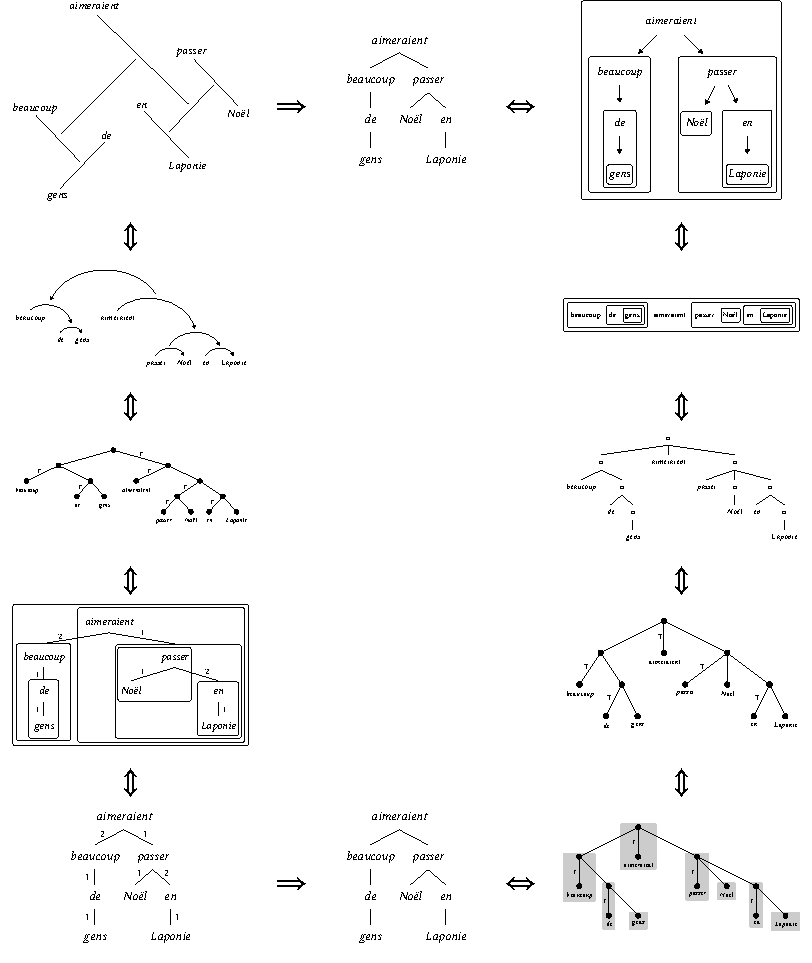
\includegraphics[width=\textwidth]{figures/graphs-collection.pdf}}

% add all extra packages you need to load to this file
\usepackage{tabularx}
\usepackage{url}
\urlstyle{same}

\usepackage{listings}
\lstset{basicstyle=\ttfamily,tabsize=2,breaklines=true}

\usepackage{enumitem}

\usepackage[linguistics,edges]{forest}
\usetikzlibrary{matrix,
                arrows,
                arrows.meta,
                graphs,
                graphs.standard,
                decorations.pathreplacing,
                fit,
                patterns,
                3d,
                perspective,
                backgrounds}

\newfontfamily\cjkfont
  [Scale=MatchLowercase,BoldFont=SourceHanSerifSC-Bold.otf]{SourceHanSerifSC-Regular.otf}
\AdditionalFontImprint{Source Han Serif}

\newfontfamily\arfont
  [Scale=MatchLowercase]{Amiri-Regular.ttf}
\AdditionalFontImprint{Amiri}

% \usepackage{showframe}
\let\clipbox\relax
\usepackage{adjustbox}

%%%%%%%%%%%%%%%%%%%%%%%%%%%%%%%%%%%%%%%%%%%%%%%%%%%%
%%%                                              %%%
%%%           Examples                           %%%
%%%                                              %%%
%%%%%%%%%%%%%%%%%%%%%%%%%%%%%%%%%%%%%%%%%%%%%%%%%%%%
%% to add additional information to the right of examples, uncomment the following line
% \usepackage{jambox}
%% if you want the source line of examples to be in italics, uncomment the following line
% \renewcommand{\exfont}{\itshape}
\usepackage{langsci-optional}
\usepackage{langsci-lgr}
\usepackage{pgfplots,pgfplotstable}
\usepackage{langsci-gb4e}
\graphicspath{{figures/}}
\usepackage{./langsci-tbls}
\usepackage{hhline}
\usepackage{floatrow}

%% hyphenation points for line breaks
%% Normally, automatic hyphenation in LaTeX is very good
%% If a word is mis-hyphenated, add it to this file
%%
%% add information to TeX file before \begin{document} with:
%% %% hyphenation points for line breaks
%% Normally, automatic hyphenation in LaTeX is very good
%% If a word is mis-hyphenated, add it to this file
%%
%% add information to TeX file before \begin{document} with:
%% %% hyphenation points for line breaks
%% Normally, automatic hyphenation in LaTeX is very good
%% If a word is mis-hyphenated, add it to this file
%%
%% add information to TeX file before \begin{document} with:
%% \include{localhyphenation}
\hyphenation{
Dub-lin
}
\hyphenation{
Dub-lin
}
\hyphenation{
Dub-lin
}
\let\hspaceThis\hphantom


\DefineBibliographyExtras{french}{\restorecommand\mkbibnamefamily}
\newcommand{\appref}[1]{Appendix \ref{#1}}
\newcommand{\fnref}[1]{Footnote \ref{#1}}
\renewcommand{\sectref}[1]{section~\ref{#1}}

\newcommand*{\Boite}{\bgroup\normalfont\ttfamily ▢\egroup}

\tcbuselibrary{theorems}

\newcommand*{\FurtherReading}[1]
  {%
    \vskip\baselineskip
    \begin{refsection}
    \nocite{*}
    \printbibliography[heading=none,keyword={Ch-#1}]
    \end{refsection}
  }

\newtcbtheorem[number within=chapter]
  {definition}
  {Définition}
  { 
    graphical environment = tikzpicture,
    boxsep = 0pt,
    fonttitle = \normalsize\sffamily\bfseries,
    toptitle = 5mm,
    top = 5mm,
    bottom = 5mm,
    left = 5mm,
    right = 5mm,
    frame engine = path,
    frame style = {fill=black!12},
    sharp corners = all,
    before upper = {\hspace*{-\parindent}}
  }
  {def}


\newcommand{\Definition}[2]{%
  \begin{definition}{#1}{}
  #2
  \end{definition}%
}

\newfontfamily\xitsfont
	  [
	    Scale=MatchLowercase,
      ]
      {XITSMath-Regular.otf}
\AdditionalFontImprint{XITS Math}

\setlength{\epigraphwidth}{.618\textwidth}% (Golden ratio)
\tikzset
  {
    reset shape/.style = {
      shape=rectangle,
      draw=none,
      fill=none
    },
    AbsSet/.style = {
      draw,
      circle,
      inner sep=9pt
    },
    ConcSet/.style = {
      draw,
      ellipse,
      font = {\itshape\strut}
    },
    EdgeLabel/.style = {
      midway,
      above,
      sloped,
      font=\small
    },
    every loop/.style={
        -{Triangle[]},
        out=120,
        in=60
    },
    FnEdgeLabel/.style={
      reset shape,
      font=\footnotesize
    },
    CircleNode/.style={
      circle, 
      draw,
      inner sep=2.5pt,
    },
    ConversionArrow/.style={
      double, 
      -{Triangle[open]}
    }
  }% exceptions for the every node/.style key

\newenvironment{langscibars}{\begin{axis}[ybar,xtick=data, xticklabels from table={\mydata}{pos},
        width  = \textwidth,
	height = .3\textheight,
    	nodes near coords,
	xtick=data,
	x tick label style={},
	ymin=0,
        ]}{\end{axis}}

\newcommand{\langscibar}[1]{\addplot+ table [x=i, y=#1] {\mydata};\addlegendentry{#1};}

\newcommand{\langscidata}[1]{\pgfplotstableread{#1}\mydata;}


\newcommand{\textstylePhono}[1]{#1}
\newcommand{\textstylePhonoApprofondissement}[1]{#1}
\newcommand{\textstylest}[1]{#1}
\newcommand{\textstyleTermes}[1]{\textsc{#1}}
\newcommand{\textstyleTermesapprof}[1]{\textsc{#1}}
\newcommand{\textstyleTermesapprofondissement}[1]{\textsc{#1}}

\newenvironment{styleExemplesuite}{}{}
\newenvironment{styleillustrationAFaire}{\begin{exe}\ex}{\end{exe}} %this seems to be object language material, which should be set off from surrounding text

\newenvironment{styleLivreImportant}{%
\begin{tblsfilled}{}
}{
\end{tblsfilled}%
}

\newenvironment{styleTitreChapitre}{}{}
\newenvironment{styleTitrePartie}{}{}
\newenvironment{styleTitreSection}{}{}
\newenvironment{styleTitreSousSection}{}{}

\newenvironment{styleaprofondissementInterTitre}{\color{red}}{}

%%%%%%%%%%%%%%%%%%%%%

\setlength{\marginparwidth}{24pt}
\KOMAoptions{headings=optiontotocandhead}
\newcommand{\gkchapter}[2]{#1: #2}
\newcommand{\gkboxsection}[3]{\section[#2]{#2\protect\marginpar{\protect\adjustbox{valign=c}{\includegraphics[width=24pt]{figures/#1.pdf}}}}#3}
% \renewcommand{\gkboxsection}[3]{\section{#2}#3}
\newcommand{\encadref}[1]{encadré~\ref{#1}}

\newcommand{\loupe}[2]{\gkboxsection{tbls-loupe}{#1}{#2}}
\newcommand{\eiffel}[2]{\gkboxsection{tbls-eiffel}{#1}{#2}}
\newcommand{\globe}[2]{\gkboxsection{tbls-world}{#1}{#2}}
\newcommand{\chevalier}[2]{\gkboxsection{tbls-history}{#1}{#2}}
\newcommand{\maths}[2]{\gkboxsection{tbls-math}{#1}{#2}}

\newcommand{\corrections}[1]{\begin{tblsfilledsymbol}{Corrections des exercices}{checkmark}#1\end{tblsfilledsymbol}}
\newcommand{\exercices}[1]{\begin{tblsfilledsymbol}{Exercices}{pencil}#1\end{tblsfilledsymbol}}
\newcommand{\exercice}[1]{\paragraph*{Exercice #1}}
\newcommand{\corrigé}[1]{\paragraph*{Corrigé #1}}
\newcommand{\citations}[1]{\begin{tblsfilledsymbol}{Citations originales}{quote}#1\end{tblsfilledsymbol}}
\newcommand{\lecturesadditionnelles}[1]{\begin{tblsfilledsymbol}{Lectures additionnelles}{book}#1\end{tblsfilledsymbol}}


\newcommand{\HappySmiley}{\bgroup\fontspec[Scale=MatchUppercase]{DejaVuSansMono.ttf}☺\egroup}
\newcommand{\SadSmiley}{\bgroup\fontspec[Scale=MatchUppercase]{DejaVuSansMono.ttf}☹\egroup}
\newcommand{\CryingSmiley}{\bgroup\fontspec[Scale=MatchUppercase]{DejaVuSansMono.ttf}😭\egroup}

\addbibresource{localbibliography.bib}

%%%%%%%%%%%%%%%%%%%%%%%%%%%%%%%%%%%%%%%%%%%%%%%%%%%%
%%%             Frontmatter                      %%%
%%%%%%%%%%%%%%%%%%%%%%%%%%%%%%%%%%%%%%%%%%%%%%%%%%%%


\begin{document}

% % \listoftodos
\maketitle
\frontmatter
\tableofcontents
\newpage\tcblistof[\chapter*]{encadre}{Table des encadrés}
\mainmatter

%%%%%%%%%%%%%%%%%%%%%%%%%%%%%%%%%%%%%%%%%%%%%%%%%%%%
%%%             Chapters                         %%%
%%%%%%%%%%%%%%%%%%%%%%%%%%%%%%%%%%%%%%%%%%%%%%%%%%%%

\chapter{Introduction}

\epigraph{DE LA SYNTAXE \textit{Ou la manière de joindre ensemble les parties d’oraison} [= les parties du discours ou catégories lexicales] \textit{selon leurs divers régimes.}

Ces diverses parties font pour ainsi dire par rapport à une langue, ce que font les matériaux, par rapport à un édifice : quelque bien préparés qu’ils soient ils ne feront jamais un palais ou une maison, si on ne les place conformément aux règles de l’architecture. C’est donc la syntaxe qui donne la forme au langage, et c’est la partie la plus essentielle de la grammaire.}{Buffier (\citeyear{buffier1709grammaire} : 294) (nous modernisons l’orthographe)}

\section{De quoi parle ce livre ?}\label{sec:0.0.0}

En commençant cet ouvrage, nous souhaitions écrire un ouvrage d’introduction à la \textstyleTermes{syntaxe de dépendance}. La plupart des ouvrages récents en syntaxe s’appuient sur l’\textstyleTermes{analyse en constituants} qui a dominé la seconde moitié du 20\textsuperscript{e} siècle. Et si les grammaires de dépendance ont connu un renouveau et un développement extraordinaire depuis le début du 21\textsuperscript{e} siècle, jusqu’à supplanter quasi totalement les grammaires de constituants dans le domaine du traitement automatique des langues (TAL), elles ne sont encore que sporadiquement enseignées à l’université et l’unique ouvrage de référence reste souvent l’ouvrage fondateur de Lucien Tesnière publié en \citeyear{tesniere1959elements}. Les \textit{Éléments} \textit{de syntaxe structurale} de Tesnière sont un incontestable monument de la littérature scientifique en linguistique, dont on ne peut que recommander la lecture, mais cet ouvrage ne peut évidemment pas prendre en compte les développements important qu’a connu le domaine depuis 60 ou 80 ans. (Tesnière est mort en 1954, il a été très malade après la guerre et ses idées ont peu évolué depuis l’édition de son polycopié \textit{Esquisses de syntaxe structurale} distribué aux élèves de l’École normale d’institutrices de Montpellier en 1943, voire de son article de \citeyear{tesniere1934comment} \textit{Comment construire une syntaxe}.)

Au final, le livre que vous avez entre les mains n’est pas un manuel sur la syntaxe de dépendance, dans le sens où il \textbf{ne} souhaite \textbf{pas} livrer de recettes qui permettront au lecteur d’\textbf{apprendre} à associer un arbre de dépendance à n’importe quel énoncé et de discuter les différentes analyses possibles d’une construction donnée \textbf{dans un cadre préconçu}. L’objectif de ce livre est au contraire de \textbf{s’interroger} \textbf{sur le cadre lui-même}, de mettre en question la validité d’une approche de la syntaxe en termes de dépendance et au-delà de cela de \textbf{définir les principes} mêmes qui doivent présider à une construction théorique en syntaxe.

Il en découle que cet ouvrage n’est pas vraiment un ouvrage d’introduction : même s’il tente d’élaborer son objet à partir de rien et qu’il est donc en théorie accessible sans pré-requis, cet ouvrage fait certainement appel à une \textbf{maîtrise du raisonnement scientifique} qui ne s’acquière qu’avec l’expérience. On pourra comparer, toutes choses égales par ailleurs, une tentative de ce genre à celle du groupe de mathématiciens français rassemblés sous le pseudonyme de Nicolas Bourbaki qui rédigea un ouvrage de construction des mathématiques à partir de rien (le premier tome démarre par la construction des entiers à partir du seul ensemble vide). L’œuvre de Nicolas Bourbaki, si elle est élémentaire au sens premier du terme (comme le souligne son titre, \textit{Éléments} \textit{de mathématiques}), s’avère d’une lecture bien difficile pour des non-mathématiciens.

Ce livre n’est pas non plus vraiment un ouvrage d’introduction à la syntaxe de dépendance, puisqu’une grande partie de l’ouvrage est consacrée à \textbf{définir l’objet} \textbf{même d’un} \textbf{ouvrage de syntaxe} et que la dépendance n’y est introduite qu’après une discussion détaillée sur les \textbf{unités de base de la syntaxe}. De plus, une large place est faite aux autres \textbf{représentations possibles de l’organisation} \textbf{syntaxique} et à la comparaison entre les différents modes de représentation. Nous pensons notamment que ceux qui travaillent en syntaxe de constituants en apprendront beaucoup sur les représentations qu’ils ont l’habitude d’utiliser et sur les \textbf{choix qui président à de telles représentations}.

Nous allons préciser l’objectif de cet ouvrage. Avant cela, le lecteur qui n’est pas familier avec la notion d’arbre de dépendance pourra consulter l’encadré qui suit. Dans la suite de l’ouvrage nous mettrons souvent des portions de texte en exergue de cette façon.

\newpage

\loupe{Arbre de dépendance}{
    Tout au long de cet ouvrage, nous proposerons de petits encadrés. Certains anticipent un peu sur la suite de l’ouvrage ; celui-ci permet à un lecteur totalement néophyte d’avoir une première idée de ce qu’est la \textstyleTermesapprof{syntaxe de dépendance}. De manière générale, les encadrés contiennent des informations complémentaires, généralement plus techniques ou à visée historique, qui ne sont pas essentielles à la compréhension du texte principal.

    L’arbre de dépendance est une représentation de la structure syntaxique devenue traditionnelle après la publication en 1959 de l’ouvrage de Lucien Tesnière, \textit{Éléments} \textit{de syntaxe structurale}, et les différents travaux qui ont suivi, notamment ceux des pragois autour de Petr Sgall, ceux des Russes autour d’Igor Mel’čuk, ainsi que des travaux en Allemagne, en Angleterre ou aux. États-Unis (mais étonnamment aucun travail significatif en France jusqu’aux années 1990).

    Dès le début de son ouvrage, Tesnière dit :

    \begin{quote}
    «~Tout mot qui fait partie d’une phrase cesse par lui-même d’être isolé comme dans le dictionnaire. Entre lui et ses voisins, l’esprit aperçoit des \textbf{connexions}, dont l’ensemble forme la charpente de la phrase.~»
    \end{quote}



\noindent   (Voir l’\encadref{sec:3.3.2} pour un \textit{Historique des notions de dépendance et de tête}, où l’on verra que cette idée est déjà dans un article de l’\textit{Encyclopédie} par Dumarsais en 1754 et que Tesnière a eu de nombreux prédécesseurs.) Tesnière ajoute ensuite que ces connexions sont orientées, liant un gouverneur à un dépendant, et forment ainsi une structure hiérarchique. C’est ce que Tesnière appelait un \textstyleTermesapprof{stemma} et qu’on appelle aujourd’hui un \textstyleTermesapprof{arbre de dépendance} (voir l’\encadref{sec:1.2.3} sur \textit{Graphe et arbre}). Ainsi l’arbre de dépendance généralement proposé pour une phrase comme :

    \ea
    \textit{Beaucoup de gens aimeraient passer Noël en Laponie}.
    \z

 \noindent   est :
    
    \ea
    \begin{forest} for tree={font=\itshape}
    [aimeraient,s sep=1.5cm
        [beaucoup,edge label={node[near start,left=1.5em,font=\normalfont\footnotesize]{sujet}}
          [de,edge label={node[midway,left,font=\normalfont\footnotesize]{complément}}
            [gens,tier=word,edge label={node[midway,left,font=\normalfont\footnotesize]{complément}}]
          ]
        ]
        [passer,edge label={node[near start,right=1.5em,font=\normalfont\footnotesize]{objet}}
          [Noël,edge label={node[near start,left=.5em,font=\normalfont\footnotesize]{objet}}] 
          [en,edge label={node[near start,right=.5em,font=\normalfont\footnotesize]{locatif}}
            [Laponie,tier=word,edge label={node[midway,right,font=\normalfont\footnotesize]{complément}}]
          ]
        ]
    ]    
    \end{forest}
    \z
    
    Dans cette représentation, les mots dépendent les uns des autres. Le mot le plus important, le verbe principal, est \textit{aimeraient}, qui occupe la racine de l’arbre et est placé tout en haut (l’arbre «~pousse~» à l’envers). Les dépendances sont étiquetées par des relations syntaxiques. Ainsi l’arbre nous dit que le sujet de \textit{aimeraient} est le groupe \textit{beaucoup de gens} et que le mot le plus important de ce groupe est \textit{beaucoup}, qui se retrouve ainsi lié à \textit{aimeraient}.

    Nous ne justifierons pas ici cette représentation, dont on peut d’ailleurs contester certains choix. Cela sera très largement discuté dans cet ouvrage et en particulier dans le \chapref{sec:3.3} sur \textit{Tête et dépendance}. Il s’agit juste de donner un premier exemple en vue de la discussion qui va suivre.
}

\section{Les questions qui nous préoccupent}\label{sec:0.0.2}

En écrivant cet ouvrage, nous nous sommes posé un grand nombre de questions auxquelles il nous a semblé qu’il fallait répondre avant de pouvoir présenter de façon objective la syntaxe de dépendance.

\begin{itemize}
\item Est-il justifié de représenter la structure syntaxique par un arbre de dépendance ? Par une structure arborescente ? Par des dépendances ? Jusqu’à quel point une représentation basée sur la dépendance est-elle ou non équivalente à d’autres modes de représentation et notamment aux arbres de constituants ?
\item Quel est le statut de la structure syntaxique ? Est-ce un objet de la langue ou bien un artefact de la modélisation des langues ? Quel rôle souhaite-t-on donner à de telles structures à l’intérieur du modèle d’une langue ?
\item Les dépendances syntaxiques sont-elles entre les mots ? Quelles sont les unités minimales de la syntaxe ? Comment définir le mot et quel rôle joue-t-il dans la syntaxe s’il n’est pas l’unité minimale de la syntaxe ?
\item Les dépendances syntaxiques s’arrêtent-elles à la frontière de la phrase ? La notion de phrase est-elle légitime ? Y a-t-il une unité maximale de la syntaxe ?
\item De quelles propriétés des énoncés cherche-t-on à rendre compte par un arbre de dépendance ? De quelles propriétés ne rend-on pas compte ? Comment encoder les propriétés qui ne sont pas prise en compte par l’arbre de dépendance ? Quelles sont les autres structures que l’on peut associer à un énoncé ? Quels rapports y a-t-il entre les différentes représentations de la structure d’un énoncé ?
\item Finalement, qu’appelle-t-on la syntaxe ? Et en quoi est-il possible ou non, nécessaire ou non, d’introduire une structure syntaxique pour rendre compte des propriétés syntaxiques d’un énoncé ? La modélisation du lien entre signifiant et signifié a-t-elle besoin d’une structure syntaxique intermédiaire ?
\end{itemize}

Toutes ces questions nous amèneront à commencer par rappeler les objectifs de notre discipline, la linguistique, et de sa sous-discipline, la syntaxe. Ces objectifs sont pour nous de \textbf{construire des modèles} des différentes langues du monde au sein d’un théorie de la langue. Notre première partie sera donc consacrée à définir les objectifs de la modélisation des langues et à montrer l’existence d’un ensemble de propriétés qui relèvent de ce que nous appelons la syntaxe.

On définit traditionnellement la syntaxe comme «~ l’étude de l’organisation des mots dans la phrase~». Une telle définition est problématique, puisqu’elle suppose que l’on peut définir les notions de mot et de phrase avant de définir ce qu’est la syntaxe. Dans cet ouvrage, la notion de mot ne sera définie qu’au début de la quatrième partie et l’unité maximale de la syntaxe ne sera discutée que dans la sixième et dernière partie de l’ouvrage.

Avant d’étudier l’organisation syntaxique, nous tenterons de \textbf{caractériser la syntaxe} et notamment les unités minimales de la syntaxe, que nous contrasterons avec les unités minimales de la morphologie et de la sémantique. Ce sera notre deuxième partie.

La troisième partie montrera comment définir une structure qui rend compte des principales propriétés syntaxiques des énoncés. Différentes structures seront présentées et la représentation par un arbre de dépendance sera particulièrement discutée.

Les trois parties suivantes s’apparentent davantage à un manuel traditionnel. Nous y présenterons différentes caractéristiques des langues et notamment du français et nous présenterons les structures qui en rendent le mieux compte. On notera néanmoins que les catégories syntaxiques et autres parties du discours, qui sont généralement introduites très tôt dans les ouvrages de syntaxe, ne seront réellement définies que dans les quatrièmes et cinquièmes parties, quand la question de l’organisation des unités aura été largement discutée.

Nous précisons le plan de cet ouvrage dans la \sectref{sec:0.0.8}.

\section{À qui s’adresse cet ouvrage ?}\label{sec:0.0.3}

Cet ouvrage aborde la syntaxe comme une \textbf{composante d’un} \textbf{modèle lingui\-stique}. L’idée même que la langue puisse être modélisée, comme peut l’être le mouvement des planètes ou le développement du fœtus, n’est pas nécessairement acceptée par tous ceux qui s’intéressent aux langues et prennent du plaisir à les apprendre ou les étudier. Cet ouvrage souhaite montrer qu’on peut dégager de manière méthodique les propriétés des langues, mettre de l’ordre dans la forêt vierge que constitue chaque langue et élaborer un objet théorique qui reproduise certaines propriétés d’un locuteur qui parle et que nous appelons un modèle d’une langue.

Il existe en linguistique, comme ailleurs en sciences humaines, des courants théoriques variés, plus ou moins d’accord entre eux. Cet ouvrage ne se situe pas précisément dans un courant dominant en linguistique, mais il puise largement dans le courant structuraliste qui s’est développé depuis un siècle, des travaux pionniers de Ferdinand de Saussure aux travaux actuels en linguistique formelle, en passant par les travaux précurseurs d’Otto Jespersen, ceux des distributionnalistes américains, Leonard Bloomfield en tête, et ceux de Lucien Tesnière et d’Igor Mel’čuk en syntaxe de dépendance. Les auteurs de ce livre ont une formation initiale en mathématiques et ont travaillé dans le domaine du traitement automatique des langues, des grammaires formelles et de la modélisation mathématique des langues et ils enseignent la linguistique à tous les niveaux universitaires. Bien que cet ouvrage ne traite pas directement de formalisation mathématique et d’implémentation informatique, il se place dans le cadre d’une \textbf{approche déductive de la langue} dont l’objectif est de construire des modèles qui peuvent être formalisés et implémentés pour simuler un locuteur humain. Ce n’est néanmoins pas l’objectif de ce livre de présenter des modèles de la langue ; ce livre se contente d’introduire, de la façon la plus rigoureuse possible, les notions nécessaires à l’étude de la syntaxe, en se concentrant sur les structures syntaxiques et non sur les règles de la grammaire.

Cet ouvrage a une visée à la fois \textbf{scientifique} et \textbf{pédagogique~}: il a été élaboré avec l’objectif de fournir une base pour l’enseignement de la syntaxe à l’université et de présenter des notions fondamentales pour l’étude des langues, aussi diverses soient-elles. Nous espérons qu’il montre qu’il est utile d’enseigner la syntaxe pour comprendre le fonctionnement des langues et mieux les enseigner et les apprendre. Cet ouvrage souhaite également montrer que la syntaxe est un domaine de recherche vivant et que de nombreuses questions restent ouvertes, même pour des langues très étudiées comme le français.

Cet ouvrage écrit en français est évidemment destiné aux francophones et à ceux qui apprennent le français. Le français constituera donc la langue que nous étudierons par défaut. Bien que cet ouvrage ne soit pas une grammaire méthodique du français, il constitue une bonne introduction à la \textbf{syntaxe du français}. Mais il souhaite aussi fournir les outils nécessaires à l’étude d’autres langues, même très éloignées du français. À chaque fois que cela sera utile, nous montrerons le caractère exotique du français dans la \textbf{diversité des langues} et présenterons pour la notion étudiée un fonctionnement différent de celui du français dans une autre langue.



\loupe{La syntaxe et les autres domaines de la linguistique}{
    La syntaxe n’est qu’une partie d’un modèle linguistique, bien que dans beaucoup de théories linguistiques, elle occupe une place centrale ou même dominante par rapport aux autres domaines. Avant de préciser ce qu’est la syntaxe, nous allons situer celle-ci parmi les autres domaines de la linguistique. Nous allons le faire en répondant à différentes questions que l’on peut se poser concernant la langue.

    Comment fonctionne l’esprit ? Comment fonctionne le raisonnement ? Comment les modéliser, les imiter ?

    Ce genre de questions appartient à la \textbf{psychologie}, la \textbf{neurologie}, la \textbf{logique}, l’\textbf{intelligence artificielle}, mais on peut espérer que de nouvelles connaissances en linguistique éclaireront aussi ces sujets. En quelque sorte, la linguistique peut être considérée comme un sous-domaine de chacune des disciplines citées : elle couvre les questions liées à la langue qui se posent dans ces sciences. Parfois, on classe toute cette thématique sous le terme de \textbf{sciences cognitives}.

    Que veut dire le dernier énoncé que j’ai entendu ? Comment ai-je pu en extraire le sens ? Comment combiner le sens des mots pour former le sens des énoncés ? Ou en quoi la phrase « \textit{Paul et Marie porte un chapeau} » se distingue-t-elle de la phrase «~\textit{Paul et Marie porte une machine à laver} » ?

    Ces questions caractérisent la \textbf{sémantique}. Même si elles ne relèvent pas directement de la syntaxe, nous les aborderons à plusieurs reprises, pour mieux délimiter la syntaxe, mais aussi parce que la syntaxe s’articule directement avec la sémantique.

    Pourquoi dit-on telle ou telle phrase dans un contexte particulier ? Quelle est la signification d’un énoncé dans un contexte ? Dans des termes plus techniques : quel est le but de l’acte de langage et comment est-il poursuivi ? Concrètement : pourquoi doit-on donner à la question « \textit{Vous avez l’heure ?}~» la réponse « \textit{Il est trois heures}~» et pas la réponse «~\textit{Oui}~» ?

    Ces questions font partie de la \textbf{pragmatique} et se situent au-delà de la sémantique. Nous n’y toucherons pas.

    Dans quel ordre doit-on placer les mots ? Quand doit-on utiliser un verbe ou un nom ? A-t-on le droit de coordonner des pronoms interrogatifs ? Quel type de structure forment les mots assemblés en une phrase ?

    Celles-ci et beaucoup d’autres questions que nous étudions dans ce livre concer\-nent la \textbf{syntaxe}.

    Comment représenter et récupérer l’information sur le fonctionnement de chaque mot ? Pourquoi dit-on \textit{une peur \textbf{bleue}}, mais \textit{\textbf{vert} de peur} ?

    Ces informations sont dans le lexique. La \textbf{lexicologie} est la science qui étudie le lexique. Nous aborderons ces questions dans la mesure où les particularités lexicales ont une influence sur la syntaxe et où la frontière entre les constructions syntaxiques et le lexique proprement dit est plus que mouvante. La question est discutée avec plus de détails dans la section suivante.

    Comment sont formés les mots ? De quelles entités sont-ils formés ? Pourquoi peut-on dire \textit{désespéré} et non \textit{désattendu} ? Comment se forme la 2\textsuperscript{e} personne singulier du passé simple pour le verbe \textsc{aimer} ?

    La \textbf{morphologie} tente de répondre à ces questions. Nous verrons qu’une partie de ces questions relèvent pour nous de la syntaxe (par exemple la conjugaison des verbes).

    Quels sont les sons d’une langue ? Quelles sont les combinaisons possibles de ces sons ? Par exemple, pourquoi les Espagnols mettent-ils des \textit{e} devant chaque mot dont l’équivalent français commence par \textit{sp} comme \textit{especial} ? Pourquoi les Français prononcent-ils \textit{ze} au lieu de \textit{the} quand ils parlent anglais ? Dans la phrase « \textit{Le fromage, je n’aime vraiment pas} », pourquoi la mélodie monte-t-elle sur le mot \textit{fromage} ? Comment est représentée la prononciation d’un mot dans le cerveau ?

    La \textbf{phonologie} s’interroge sur ces questions. Nous les aborderons dans la mesure où la structure phonologique des énoncés nous offre de nombreux indices sur la structure syntaxique des énoncés et où la langue parlée constitue, du notre point de vue, un bien meilleur sujet d’étude que la langue écrite.

    Comment sont réellement formés les sons de la langue ? Comment se distingue un son [d] d’un son [z] ? Pourquoi y a-t-il une différence entre un son [k] prononcé devant [i] et un son [k] prononcé devant [u] ? Comment se distingue le son [a] de l’allemand du son [a] du français ?

    S’il s’agit de répondre à ces questions en termes de fonctionnement de la langue et de l’humain produisant les sons, on se trouve dans la \textbf{phonétique} (articulatoire), si c’est en termes purement techniques et physiques, c’est plutôt l’\textbf{acoustique} et le \textbf{traitement du signa}l, un domaine relevant de la physique, qui sont concernés.

    Il existe d’autres domaines en linguistique, notamment tout ce qui concerne la langue dans ses variations dans le temps et dans l’espace : sociolinguistique, géolinguistique, dialectologie, diachronie, origine du langage, génétique des langues, grammaticalisation, créolisation, productivité lexicale, acquisition de la langue par l’enfant, apprentissage d’une langue seconde. Il existe aussi de nombreux domaines d’application : le traitement automatique des langues ou TAL (traduction automatique, recherche d’information sur le web ou dans des bases de données, aide aux handicapés, synthèse de la parole), l’enseignement de la langue (Français Langue Étrangère ou FLE pour les apprenants langue seconde, la didactique des langues pour les écoliers francophones), etc. Dans les champs interdisciplinaires, nous trouvons la psycholinguistique, la sociolinguistique, la neurolinguistique, la linguistique textuelle, la linguistique mathématique, etc.
}

\section{Grammaire et lexique}\label{sec:0.0.5}

Lorsqu’un locuteur veut énoncer une idée dans sa langue, il doit trouver dans son \textstyleTermes{lexique} les unités lexicales qui correspondent le mieux aux entités dont il veut parler. Mais, pour former la phrase, le locuteur a besoin d’autres éléments linguistiques qui sont contraints de diverses façons par la langue. L’étude de ces éléments et des contraintes que la langue impose à un locuteur s’appelle la \textstyleTermes{grammaire} de cette langue.

En fait, la frontière entre lexique et grammaire n’a rien d’évident. La description d’une langue est la description de chacune des unités de la langue et de la façon dont elles se combinent. Parmi ces unités, on trouve des unités lexicales prototypiques comme \textsc{cheval} ou \textsc{manger}, tandis que d’autres sont des unités grammaticales incontestables comme le temps imparfait (\textit{Le cheval mange}\textbf{\textit{ai}}\textit{t}) ou les différentes réalisations syntaxiques du pluriel (\textit{L}\textbf{\textit{es}} \textit{chev}\textbf{\textit{aux}} \textit{mangeai}\textbf{\textit{ent}}). Mais d’autres unités, tout en partageant des propriétés avec les unités lexicales prototypiques ont aussi un fonctionnement grammatical, comme \textsc{chose} ou \textsc{faire} (\textit{La} \textbf{\textit{chose}} \textit{que je préfère, c’est manger~}; \textit{Ce que je préfère} \textbf{\textit{faire}}, \textit{c’est manger}). Inversement, des unités qui ont un fonctionnement a priori grammatical, comme la préposition \textsc{à} dans \textit{Elle parle} \textbf{\textit{à}} \textit{Pierre}, auront un fonctionnement beaucoup plus lexical lorsqu’elles commutent avec d’autres unités : \textit{Elle est} \textbf{\textit{à}} \textit{la maison,} \textbf{\textit{dans}} \textit{la maison,} \textbf{\textit{devant}} \textit{la maison,} \textbf{\textit{derrière}} \textit{la maison}, etc.

La distinction entre lexique est grammaire est orthogonale à la partition du modèle linguistique entre morphologie, syntaxe et sémantique. Toutes les unités, qu’elles soient lexicales ou grammaticales, possèdent une forme, un sens et une combinatoire qu’il faut décrire (voir la \sectref{sec:2.1.3} sur \textit{Signifié, signifiant, syntactique}). La \textstyleTermes{syntaxe} est l’étude de la \textbf{combinatoire des unités lexicales et grammaticales} et tout particulièrement des combinaisons libres obéissant à des règles générales. La syntaxe se trouve à mi-chemin de la \textstyleTermes{sémantique} qui s’intéresse au \textbf{sens} des unités lexicales et grammaticales et des énoncés qu’elles forment en se combinant et de la \textstyleTermes{morphologie} qui s’intéresse à la \textbf{forme} et la structure des unités que la syntaxe combine.

\loupe{Notations}{
    Nous notons nos \textit{exemples linguistiques} en italiques. Pour les \textsc{unités lexicales}, nous utilisons des petites capitales. Lorsqu’il s’agit d’unités lexicales multi-mots comme $⌜$\textsc{pomme de terre}$⌝$, nous utilisons des balises angulaires. Les unités grammaticales sont quant à elles généralement désignées par des termes métalinguistiques : présent, singulier, féminin, etc. Le sens d’une unité lexicale ou d’une portion de texte est indiqué en guillemets simples : ‘cheval’, ‘pomme de terre’, ‘le cheval mange’. La signification d’une unité grammaticale est également noté entre guillemets, mais en mettant le terme en petites capitales : ‘\textsc{singulier’}. On ne confondra pas le sens grammatical ‘\textsc{présent’} qui signifie ‘ayant lieu maintenant’ avec le sens lexical ‘présent’.
}

\eiffel{Le lexique : un cabinet de curiosités}{
    Bien que la syntaxe et la grammaire soient au centre de cet ouvrage, on ne peut pas ne pas évoquer la complexité lexicale dans un tel ouvrage. Nous allons en donner trois exemples.

    Chaque verbe impose à ses compléments une construction particulière : \textit{manger quelque chose, parler} \textbf{\textit{à}} \textit{quelqu’un} \textbf{\textit{de}} \textit{quelque chose, donner quelque chose} \textbf{\textit{à}} \textit{quelqu’un, compter} \textbf{\textit{sur}} \textit{quelqu’un, aller quelque part, poser quelque chose quelque part}, etc. Ces constructions se comptent en dizaines. Même lorsque ces constructions semblent similaires, comme \textit{parler à quelqu’un} et \textit{penser à quelqu’un}, elles peuvent différer par leur comportement : ainsi, \textit{à Marie, je lui parle, j’y pense} ou \textit{je pense à elle}, mais on ne pourra pas dire *\textit{je lui pense} ou~\textsuperscript{??}\textit{je parle à elle} (pour l’utilisation des symboles * et~\textsuperscript{??}, voir la \sectref{sec:1.1.11} sur l’\textit{Acceptabilité}). Dans certains cas, le verbe contraint tellement son complément que seules quelques formes sont acceptables. C’est le cas par exemple de la tournure verbale \textit{y comprendre quelque chose}, qui n’est possible qu’avec les compléments suivants : \textit{Je n’y comprends} \textbf{\textit{rien}}, \textit{Je n’y comprends pas} \textbf{\textit{grand-chose}}, \textbf{\textit{Que}} \textit{puis-je y comprendre} ?, \textit{Y comprends-tu} \textbf{\textit{quelque chose~}}? et \textit{J’y comprends} \textbf{\textit{que dalle}}. Il est impossible d’avoir un groupe nominal référentiel comme complément : *\textit{J’y comprends une chose intéressante}. La liste des compléments possibles de cette acception de \textsc{comprendre} constitue ainsi un véritable cabinet de curiosités avec un pronom interrogatif (\textsc{quoi} et sa forme atone \textit{que}), un pronom négatif (\textsc{rien}), deux pronoms indéfinis — $⌜$\textsc{quelque chose}$⌝$ qui n’est possible ici qu’avec l’interrogation et \textsc{grand-chose} qui est toujours accompagné de la négation — et enfin $⌜$\textsc{que dalle}$⌝$. Notons que d’autres tournures verbales possèdent quasiment la même complémentation : \textit{Ça ne rime à rien, Ça ne rime pas à grand-chose, À} \textit{quoi ça rime} ?, mais pas *\textit{Ça rime à une chose intéressante} ou *\textit{Ça rime à faire ça}.

    Les exceptions lexicales sont encore plus nombreuses quand on se rapproche de la grammaire. Le français possède par exemple plusieurs éléments négatifs qui se construisent avec \textit{ne} : \textit{Je} \textbf{\textit{ne}} \textit{dors} \textbf{\textit{pas}}, \textit{Je} \textbf{\textit{ne}} \textit{dors} \textbf{\textit{plus}}, \textit{Je} \textbf{\textit{ne}} \textit{dors} \textbf{\textit{jamais}}, \textit{Je} \textbf{\textit{ne}} \textit{dors} \textbf{\textit{nulle part}}, \textit{Je} \textbf{\textit{ne}} \textit{mange} \textbf{\textit{rien}}, \textit{Je} \textbf{\textit{ne}} \textit{parle à} \textbf{\textit{personne}}, \textit{Je} \textbf{\textit{n’}}\textit{ai} \textbf{\textit{aucun}} \textit{problème, Je} \textbf{\textit{n’}}\textit{ai} \textbf{\textit{qu’}}\textit{une idée}. Chacun de ces éléments possède des propriétés syntaxiques différentes : par exemple \textsc{jamais} peut être déplacé, mais pas \textsc{pas} ou \textsc{plus~}: \textbf{\textit{Jamais}} \textit{je ne dors} vs *\textbf{\textit{Plus}} \textit{je ne dors}. \textsc{jamais} et \textsc{plus} peuvent être combinés, mais pas \textsc{jamais} et \textsc{pas~}: \textbf{\textit{Jamais plus}} \textit{je ne dormirai, Je ne dormirai} \textbf{\textit{plus jamais}} vs *\textit{Je ne dormirai} \textbf{\textit{pas jamais}}, \textit{*Je ne dormirai} \textbf{\textit{jamais pas}}. Notons encore que \textsc{rien} et \textsc{personne} se placent différemment par rapport au verbe : \textit{Je n’ai vu} \textbf{\textit{personne}}, \textit{Je n’ai} \textbf{\textit{rien}} \textit{vu}. Sans aller plus loin, on aura compris que chacun de ces éléments négatifs nécessitera une étude séparée simplement pour déterminer ses propriétés combinatoires, c’est-à-dire sa «~syntaxe~». Il en va de même de chacun des pronoms interrogatifs ou de chacun des pronoms relatifs et ainsi de la plupart des unités lexicales ayant un rôle grammatical.

    Terminons par l’exemple des \textstyleTermes{constructions}, ainsi que l’on nomme les configurations qui possèdent un rôle grammatical. Il existe en français une construction très employée, le présentatif $⌜$\textsc{il y a … qu-}$⌝$, pratiquement obligatoire à l’oral lorsque le sujet est indéfini :

    \ea
    \ea 
    \textit{\textbf{{Il y a}} {quelqu’un} \textbf{{qui}} {nous regarde depuis la fenêtre.}}
    \ex
    \textit{\textbf{{Il y a}} {des choses} \textbf{{que}} {j’ai} {achetées} {sur la table.}}
    \z
    \z

   \noindent Le présentatif peut être combiné avec la restriction en $⌜$\textsc{ne … que}$⌝$ :

   \ea
    \textit{{Il} \textbf{{n’}}{y a} \textbf{{que}} {des choses que j’ai} {achetées} {sur la table.}}
    \z

  \noindent  La combinaison du présentatif avec la restriction s’applique à des compléments indirects :

   \ea
   \ea
   \textit{ \textbf{{Il n’y} {a qu’}}{à un endroit} \textbf{{qu’}}{on les trouve.}}
   \ex
    \textit{\textbf{{Il n’y} {a qu’}}{à elle} \textbf{{que}} {je pense.}}
   \z
   \z

 \noindent  alors que le présentatif seul ne le peut pas :

   \ea
   \ea[*]\textit{{\textbf{{Il y a}} {à un endroit} \textbf{{qu’}}{on les trouve.}}}
   \ex[*]\textit{{\textbf{{Il y a}} {à quelqu’un} \textbf{{que}} {je pense.}}}
   \z
   \z

  \noindent  Lorsque le présentatif s’applique à un complément avec possessif, on peut exprimer cette possession dans la forme même du présentatif :

   \ea
    \ea \textit{\textbf{{Il y a}} {mon frère} \textbf{{qui}} {doit venir.}}
    \ex \textit{\textbf{{J’ai}} {mon frère} \textbf{{qui}} {doit venir.}}
    \z
    \z

   \noindent Enfin, la même configuration peut être utilisée pour introduire un complément de temps avec le sens ‘depuis’ :

   \ea
    \textit{\textbf{{Il y a}} {une semaine} \textbf{{qu’}}{on ne s’est} {pas vu.}}
    \z

 \noindent   Dans ce cas, elle possède une variante, mais celle-ci n’est possible que pour les compléments de temps :

   \ea
   \ea[]\textit{{\textbf{{Ça} {fait}} {une semaine} \textbf{{qu’}}{on ne s’est} {pas vu.}}}
   \ex[*]\textit{{\textbf{{Ça} {fait}} {des choses} \textbf{{que}} {j’ai} {achetées là-bas.}}}
   \z
   \z

   Comme on le voit, on retrouve pour ces constructions de nombreuses \textbf{idiosyncrasies} qui justifient de leur donner une description détaillée, au même titre que les autres unités lexicales.
    }
\section{Le plan du livre}\label{sec:0.0.8}

Ce livre est divisé en six parties que nous avons esquissées à la \sectref{sec:0.0.2} sur \textit{Les questions qui nous préoccupent}. Nous allons préciser le plan du livre.

La première partie explique en quoi consiste une \textstyleTermes{langue} et la \textstyleTermes{modélisation} de cette langue (\chapref{sec:1.1}) et quelles sont les caractéristiques du modèle linguistique que nous construisons (\chapref{sec:1.3}). Cette première partie permet donc de comprendre quel est le cadre théorique de cet ouvrage et avec quel objectif nous souhaitons mener notre étude de la langue et de sa syntaxe. La modélisation est illustrée par l’exemple de la production d’un énoncé (\chapref{sec:1.2}).

La deuxième partie pose la question des unités minimales de la langue (\chapref{sec:2.1}). Étudier la combinatoire des unités qui constituent les énoncés ne peut se faire qu’après avoir identifié les unités qui se combinent et notamment les unités minimales. Nous montrons qu’il est nécessaire de considérer trois types d’unités minimales : les \textstyleTermes{morphèmes} ou unités minimales de forme (\chapref{sec:2.2}), les \textstyleTermes{sémantèmes} ou unités minimales de sens (\chapref{sec:2.3}) et les \textstyleTermes{syntaxèmes} ou unités minimales de la syntaxe, c’est-à-dire de la combinatoire libre. La distinction de trois types d’unités résulte de la non-correspondance entre les unités de forme et de sens. Prenons un exemple :
\ea
    \textit{Les étudiants m’ont donné un coup de main.}
\z
Il y a dans cet énoncé plusieurs sémantèmes qui sont exprimés par une combinaison de morphèmes : \textit{coup de main} bien sûr, qui ne signifie pas ici un coup de la main, mais aussi \textit{étudiant}, qui combine le radical du verbe \textsc{étudier} avec le morphème -\textit{ant} ou encore le passé composé exprimé par le verbe \textsc{avoir} combiné avec le morphème de participe passé \textit{{}-é}.

La troisième partie introduit les \textstyleTermes{unités syntaxiques} et la façon dont celles-ci se combinent pour former la \textstyleTermes{structure syntaxique}. On y définit la syntaxe comme l’étude des \textstyleTermes{combinaisons libres} d’unités et on caractérise plus précisément le syntaxème (\chapref{sec:3.1}). Nous montrons que les différentes fragmentations d’un énoncé en unités syntaxiques définissent un graphe que nous appelons la \textstyleTermes{structure de connexion} et qui décrit les combinaisons entre syntaxèmes (\chapref{sec:3.2}). On peut en plus hiérarchiser cette structure en considérant la notion de \textstyleTermes{tête} d’une unité syntaxique et obtenir ainsi une \textstyleTermes{structure de dépendance} (\chapref{sec:3.3}). On montre comment représenter cette structure de manière plus ou moins équivalente par un \textstyleTermes{arbre de constituants} (\chapref{sec:3.4}). On s’intéresse ensuite au lien d’une part entre la structure et le texte et d’autre part entre la structure syntaxique et le sens. Le premier cas concerne l’ «~ordre des mots~», c’est-à-dire à la façon dont les syntaxèmes s’ordonnent les uns par rapport aux autres et se regroupent pour former des \textstyleTermes{constituants topologiques} au sein de la \textstyleTermes{structure topologique} (\chapref{sec:3.5}). Le deuxième cas concerne l’\textstyleTermes{interface} \textstyleTermes{sémantique-syntaxe}, c’est-à-dire à la façon dont les sémantèmes se combinent, ce que décrit la \textstyleTermes{structure syntaxique profonde}, qui rend compte de la distinction entre \textstyleTermes{actant} et \textstyleTermes{modifieur} et des restructurations parfois complexes entre la représentation sémantique et la structure syntaxique (\chapref{sec:3.6}).

Les trois parties suivantes présentent les trois grands domaines de la syntaxe, que nous appelons nanosyntaxe, microsyntaxe et macrosyntaxe, et les principales notions de la syntaxe seront présentées : le mot, les catégories flexionnelles, les catégories lexicales, les fonctions syntaxiques, la phrase. Les principales constructions seront également étudiées, et notamment les listes, l’extraction et l’organisation des énoncés autour d’un noyau.

La quatrième partie de ce livre est donc consacrée à la \textstyleTermes{nanosyntaxe} ou \textstyleTermes{morphosyntaxe}. Elle présente les combinaisons de \textstyleTermes{syntaxèmes} possédant une très grande cohésion, dont les composantes sont indissociables et se situent à l’intérieur ou à la frontière des mots. Elle inclut la \textstyleTermes{syntaxe flexionnelle} et la syntaxe des \textstyleTermes{particules}, c’est-à-dire la syntaxe de tous les éléments qui sont des marqueurs grammaticaux et qui possèdent très peu d’indépendance syntaxique. Nous montrons en particulier que le \textstyleTermes{mot} n’est qu’un degré particulier dans l’échelle de cohésion des combinaisons de syntaxèmes en unités syntaxiques, même s’il constitue une unité naturelle et l’unité qui a été privilégiée pour la transcription écrite de nombreuses langues (\chapref{sec:4.1}). Nous terminons cette partie par une première classification des unités minimales de la syntaxe et introduirons les \textstyleTermes{catégories flexionnelles} (\chapref{sec:4.2}) et les \textstyleTermes{catégories nanosyntaxiques} de \textstyleTermes{lexèmes} (\chapref{sec:4.3}).

La cinquième partie est consacrée à la \textstyleTermes{microsyntaxe}, c’est-à-dire la syntaxe de rection : la \textstyleTermes{rection} se caractérise par une relation hiérarchique avec des contraintes de réalisation imposées par un gouverneur à ses dépendants. Elle constitue la syntaxe \textit{par excellence.} Nous introduisons la \textstyleTermes{syntaxe de dépendance de surface} et la distinction entre les propriétés fonctionnelles et catégorielles des éléments d’un énoncé. Nous étendons le classement des syntaxèmes à l’ensemble des unités syntaxiques et étudions les \textstyleTermes{catégories microsyntaxiques} et le rôle de la \textstyleTermes{translation} (\chapref{sec:5.1}). Le classement des syntagmes nous amène à introduire la notion de \textstyleTermes{relation syntaxique}. Les différentes \textstyleTermes{fonctions syntaxiques} que peut remplir une unité sont caractérisées et notamment la fonction \textit{sujet}, qui pose problème, dès qu’on prend en compte les langues ergatives (\chapref{sec:5.2}). Une attention particulière est portée aux \textstyleTermes{listes} ou \textstyleTermes{entassements paradigmatiques} : nous regroupons sous ce terme différents phénomènes, allant de la coordination à la reformulation, où plusieurs éléments viennent occuper une même position régie (\chapref{sec:5.3}). L’étude détaillée de l’\textstyleTermes{extraction} et du rôle complexe joué par des éléments tels que les pronoms relatifs constitue le dernier chapitre de cette partie (\chapref{sec:5.4}).

La sixième partie est consacrée à la \textstyleTermes{macrosyntaxe}, c’est-à-dire l’étude de tout ce qui se situe au-delà de la microsyntaxe, notamment les éléments associés au noyau central de l’énoncé sans pour autant être régis. Nous y définissons l’\textstyleTermes{unité illocutoire} qui constitue l’unité minimale du discours et étudions son organisation interne en \textstyleTermes{noyau} et \textstyleTermes{adnoyaux}. Nous montrons pourquoi la notion traditionnelle de \textstyleTermes{phrase} est problématique, notamment parce qu’il y a de la rection au-delà des limites de l’unité illocutoire et qu’à l’inverse des unités non régies peuvent venir s’insérer à l’intérieur d’une unité illocutoire (\chapref{sec:6.1}).

\loupe{Les termes grammaire, syntaxe et topologie}{
    Le terme grec \textit{grammatikē} \textit{technē} (γραμματικὴ τέχνη) désignait « \textbf{l’art} \textbf{des lettres} », \textit{lettre} dans le sens de «~l’écrit~» ; c’était donc l’étude de l’écrit (et l’étude de sa lecture). Elle s’est ensuite développée en science de l’interprétation des textes, ce que, aujourd’hui, on classe plutôt sous le terme de \textstyleTermesapprof{philologie} et que l’on distingue de la \textstyleTermesapprof{grammaire}. Il y a 3000 ans, bien avant les Grecs, il existait déjà des études grammaticales (au sens moderne du terme) de langues telles que le sanskrit ou le chinois et au 5\textsuperscript{e} siècle avant notre ère, le grand linguiste indien Pā\textrm{ṇ}ini a développé une analyse systématique de la nanosyntaxe du sanskrit. Les \textit{Institutiones grammaticae}, écrites au 6\textsuperscript{e} siècle par le grammairien latin Priscien, auront une influence déterminante sur le développement de la grammaire en Europe. Beaucoup de termes grammaticaux encore en utilisation aujourd’hui proviennent de l’étude du latin, \textit{lingua franca} jusqu’à la fin du moyen-âge.

    Le terme \textit{syntaxis} est également grec : il est composé de \textit{syn} (συν) ‘ensemble’ \textit{et de táxis} (τάξις) ‘ordre, arrangement’. La \textstyleTermesapprof{syntaxe} a désigné l’étude de l’ordre des mots, puis plus largement l’étude de l’organisation des mots dans la phrase. Le terme allemand pour syntaxe est \textit{Satzlehre}, tout simplement la ‘science de la phrase’. Dans la conception traditionnelle, l’analyse syntaxique est limitée d’un côté par le mot, et de l’autre par la phrase : les structures en deçà du mot ne font pas partie de la syntaxe, elles appartiennent à la morphologie ; le \textbf{discours}, l’enchaînement de plusieurs phrases, n’est pas le sujet de la syntaxe, mais de la linguistique des textes ou \textstyleTermesapprof{analyse du discours}. Notre définition de la syntaxe ne présuppose ni la notion de mot, ni celle de phrase, et considère la \textstyleTermesapprof{morphologie} comme l’étude de la \textbf{combinaison des signifiants des signes} (voir la \sectref{sec:2.1.3} sur \textit{Signifié, signifiant, syntactique}).

    Les termes \textit{microsyntaxe} et \textit{macrosyntaxe} ont été forgés en 1990 par les linguistes qui se sont intéressés aux productions orales spontanées (notamment à Aix-en-Provence autour de Claire Blanche-Benveniste et à Fribourg en Suisse autour d’Alain Berrendonner) et ont vu la difficulté que pouvait poser une segmentation en phrases comme à l’écrit. Sur le même modèle, nous proposons le terme \textit{nanosyntaxe}, à la place du terme \textit{morphosyntaxe}, pour compléter la partition de l’étude de la syntaxe. Nous introduisons le terme \textit{syntaxème} pour nommer les \textbf{unités minimales} de la syntaxe, sur le même modèle que les termes \textit{morphème} et \textit{sémantème}, désignant respectivement les unités minimales de forme et de sens.

    Dans l’usage du terme \textit{syntaxe}, on est passé de l’étude de l’ordre des mots à, aujourd’hui, l’étude de la combinaison des syntaxèmes et aux structures hiérarchiques qui en résultent. Une des conséquences est qu’il fallait réintroduire un nouveau terme pour l’étude de l’\textbf{ordre des mots} et des syntaxèmes. Nous avons adopté le terme \textit{topologie}, également d’origine grecque : la \textstyleTermesapprof{topologie} est l’étude des \textit{topos} (τόπος), c’est-à-dire l’étude des lieux. Le terme a été introduit au 19\textsuperscript{e} siècle par les linguistes décrivant l’ordre des mots des langues germaniques à l’aide de gabarits de places : le \textbf{modèle topologique} de l’allemand décrit la façon dont la phrase allemande peut être décomposée en cinq \textbf{champs}, les deuxième et quatrième champs modélisant les positions réservées aux verbes (voir le \chapref{sec:3.5} sur \textit{La topologie}).
}
\section{Commentaires sur le plan}\label{sec:0.0.10}

Le plan de cet ouvrage amène plusieurs commentaires et permet déjà de se faire une idée des principaux partis pris.

On constatera tout d’abord que nous considérons trois structures «~syntaxiques~» — la structure topologique, la structure de dépendance de surface et la structure syntaxique profonde — là où la plupart des approches n’en considèrent qu’une : la structure syntagmatique ou analyse en constituants immédiats. Nous aurons plusieurs fois l’occasion de justifier le fait de séparer les informations qui peuvent l’être et donc de dissocier les différents modes d’organisation des différents types d’unités qui apparaissent dans un énoncé.

Autre point : nous donnons une place importante aux interfaces, c’est-à-dire à la correspondance entre les différents niveaux de représentation de l’énoncé. Ceci est principalement dû à notre objectif de modélisation : nous ne souhaitons pas seulement montrer comment un énoncé est structuré, mais aussi comment un locuteur produit ces différentes structures et quels rôles elles jouent dans la production des énoncés. Modéliser la langue, c’est pour nous modéliser comment une personne parle, c’est-à-dire comment elle produit des énoncés dans sa langue en fonction du message qu’elle souhaite communiquer.

La plupart des ouvrages de syntaxe et des cours de linguistique à l’université commencent par l’étude des catégories syntaxiques ou parties du discours, c’est-à-dire la caractérisation de ce qu’est un verbe, un nom, un adjectif, etc. Nous pensons pour notre part qu’une bonne définition des catégories syntaxiques ne peut se faire qu’après avoir dégagé la structure des énoncés et que la caractérisation des catégories repose sur l’analyse distributionnelle des unités syntaxiques à l’intérieur des combinaisons complexes dans lesquelles elles entrent. Autrement dit, on ne peut caractériser les catégories syntaxiques d’une langue par l’étude du simple enchaînement linéaire des unités dans la chaîne parlée : il faut prendre en compte les relations plus complexes qui lient les éléments d’un énoncé et dont l’ordre des mots en surface n’est qu’une projection. La description des liens syntaxiques est au cœur de la syntaxe de dépendance et elle occupe une place centrale dans ce livre. Les catégories syntaxiques seront définies en deux chapitres (4.3 et 5.1) distribués dans les parties consacrées à la nanosyntaxe et à la microsyntaxe.

Cette présentation assez systématique des notions utiles à la syntaxe nous a obligé à définir de nouveaux concepts ou à revoir certains concepts traditionnels. Selon les cas, nous avons décidé d’utiliser un terme déjà usuel dans un sens un peu différent ou bien nous avons forgé un nouveau terme. Parmi les néologismes que contient cet ouvrage, on notera le terme \textit{syntaxème} utilisé pour nommer les unités minimales de la syntaxe (qui curieusement ne sont jamais nommées) et \textit{nanosyntaxe} pour désigner la syntaxe des éléments qui possèdent peu d’autonomie syntaxique. Par ailleurs, d’autres termes peu fréquents dans les manuels de syntaxe occupent ici une position plus centrale, comme \textit{sémantème}, \textit{topologie, macrosyntaxe} ou \textit{syntaxe profonde}.

\loupe{Notions, termes, concepts et définitions}{
    Nous allons illustrer la distinction entre notions, termes, concepts et définitions à partir d’un exemple. Considérons la \textstyleTermesapprof{définition} suivante :

    \ea
    Une \textit{phrase} est un segment de texte qui se trouve entre deux ponctuations majeures successives.
    \z

    Un \textstyleTermesapprof{terme} est introduit : \textit{phrase}. Ce terme est associé à un \textstyleTermesapprof{concept}. Le concept est un objet abstrait, conceptuel, qui n’est accessible qu’à travers la \textstyleTermesapprof{définition} qui le caractérise, à savoir «~un segment de texte qui se trouve entre deux ponctuations majeures successives~». En associant ce terme et ce concept, nous construisons une notion. Une \textstyleTermesapprof{notion} est donc un concept nommé ou un terme défini et associé à un concept.

    La distinction entre le terme et le concept qui lui correspond est essentielle, puisqu’un même terme peut être associé par différents auteurs à différents con\-cepts. Évidemment, une fois que nous avons associé le terme \textit{phrase} à un concept, nous pouvons parler de «~la notion de phrase~», mais il faut être conscient qu’il s’agit d’un raccourci pour désigner «~la notion que nous avons nommée \textit{phrase} et qui ne doit pas être confondue avec une autre notion que d’autres ont pu également nommer \textit{phrase} et qui peut à l’inverse avoir été nommée autrement par d’autres~».

    Il y a plusieurs raisons pour lesquelles, en linguistique, la terminologie n’est pas bien stabilisée et un même terme tend à désigner des concepts divers. Une première raison est que beaucoup de ces termes (\textit{mot, phrase, nom, adverbe, sujet,} etc.) s’appliquent à des notions qui sont enseignées dès l’école et reçoivent donc des définitions simplifiées et facilement accessibles, qui deviennent inopérante lorsqu’un véritable cadre théorique est développé. Une deuxième raison est qu’il n’est pas possible de définir proprement de telles notions sans se doter d’un appareil conceptuel complexe et qu’il n’y a pas aujourd’hui de théorie consensuelle sur la nature de la langue et sur les primitives conceptuelles, c’est-à-dire les notions de base à partir desquels des notions plus complexes pourront être définies.

    Dans cet ouvrage, nous allons nous attacher à introduire un appareillage théorique rigoureux. Nous introduirons un grand nombre de concepts auxquelles nous associerons bien sûr des termes. Nous avons fait le choix d’utiliser autant que possible les termes courants en linguistique, même lorsque nous décidions de définir une notion un peu différente de la tradition. C’est par exemple le choix que nous avons fait pour le terme \textit{syntaxe}, auquel nous donnons une acception différente de la tradition. Lorsque nous avons introduit des concepts nouveaux, nous nous sommes permis d’utiliser un terme vacant s’il n’était pas trop éloigné : c’est ce que nous avons fait avec le terme \textit{substantif}, qui désignait avant ce qu’on appelle aujourd’hui \textit{nom} et que nous avons attribué à une notion du même ordre, mais différente de celle du nom (voir \chapref{sec:5.1} sur \textit{Les catégories microsyntaxiques}). Lorsqu’aucun terme ne se présentait, nous nous sommes résolus à forger un nouveau terme. Nous avons alors cherché à régulariser la terminologie. C’est ce qui nous a amené à introduire le terme \textit{syntaxème} à côté des termes \textit{morphème} et \textit{sémantème}, ou à introduire le terme \textit{nanosyntaxe} à côté des termes \textit{microsyntaxe} et \textit{macrosyntaxe}.

    On peut être en désaccord avec la définition d’une notion. Il est important de voir que ce désaccord peut se situer à trois niveaux bien différents. Revenons sur la notion qui illustre cette section. On peut être en désaccord :

    \begin{itemize}
    \item  au \textbf{niveau proprement définitionnel~}: on peut considérer que notre définition n’en est pas vraiment une, car elle comprend des termes qui n’ont pas été eux-mêmes définis. Qu’appelle-t-on une ponctuation majeure ? Le point-virgule est-il une ponctuation majeure ? Qu’entend-on exactement par un segment de texte ? S’agit-il juste d’une chaîne de caractères ou bien la phrase est-elle un signe linguistique avec un sens associé au texte proprement dit ?
    \item  au \textbf{niveau théorique ou conceptuel :} la notion définie est-elle intéressante d’un point de vue théorique ? Certainement pas si on n’élimine pas le cas des points qui suivent une abréviation, comme dans \textit{Georges W.} \textit{Bush}. Et au-delà, les unités définies par la ponctuation sont-elles bien des unités linguistiques pertinentes ?
    \item  au \textbf{niveau purement terminologique~}: est-ce bien à ce concept que l’on veut associer le terme \textit{phrase} ? Ou inversement, est-ce bien par le terme \textit{phrase} que l’on veut désigner ce concept ?
    \end{itemize}

    Les problèmes terminologiques sont secondaires : un mauvais choix de terme ne remet pas en cause une théorie. Mais ils peuvent être catastrophiques du point de vue pédagogique et rendre incompréhensible une construction théorique valable par ailleurs. Lorsqu’on introduit un concept, on a principalement deux options terminologiques : utiliser un terme existant, avec le risque que d’autres auteurs l’utilisent avec une acception différente (c’est le cas avec le terme \textit{phrase}), ou bien forger un nouveau terme, avec le risque d’avoir des termes «~barbares~» et difficiles à mémoriser. On peut par exemple proposer d’appeler le concept défini plus haut \textit{phrase graphique}. C’est ce que nous ferons dans la suite de l’ouvrage.

    Une \textit{phrase graphique} est une unité de l’écrit, un segment de texte qui se trouve entre deux ponctuations majeures successives. Les ponctuations majeures sont le point (à l’exception des points utilisés dans les abréviations), le point d’interrogation, le point d’exclamation et les trois petits points. Le point virgule segmente une phrase en sous-phrases.

    Les questions théoriques et conceptuelles sont les plus importantes : il est bien sûr crucial d’introduire les bons concepts. C’est l’ensemble des concepts introduits qui définit le cadre théorique à partir duquel un modèle d’une langue particulière pourra être élaboré. La notion de phrase que nous avons introduite est-elle vraiment la plus intéressante du point de vue linguistique ? Nous verrons que non, ne serait-ce que parce que l’écrit est une transcription de la langue et qu’une notion de l’ordre de la phrase existe indépendamment de la possibilité d’écrire ou pas (voir la \sectref{sec:1.1.2} sur les \textit{Sons et textes}).

    Les problèmes définitionnels sont immenses. En général, la définition d’une notion fait appel à d’autres notions. Il faut donc comprendre quels sont les concepts qui doivent être définis avant les autres. Dans notre exemple, nous avons défini la phrase à partir de la ponctuation. Mais comment un locuteur sait-il où mettre des ponctuations majeures quand il écrit ? Produit-on des unités de l’ordre de la phrase lorsqu’on parle ? Si oui, il existe une unité de l’ordre de la phrase plus fondamentale que celle que nous venons de définir et qui ne se définit pas en fonction de l’écrit et encore moins en fonction de la ponctuation. Si beaucoup d’ouvrages de linguistique commence par la définition de la phrase, nous considérons pour notre part qu’il s’agit d’une notion complexe qui ne peut être définie qu’après avoir introduit la notion de cohésion syntaxique. C’est la raison pour laquelle les notions proches de la phrase seront seulement discutées à la fin de cet ouvrage, dans la sixième et dernière partie. Nous verrons de ce point de vue que derrière la phrase graphique se cache en fait deux types d’unités différentes, ce qui explique qu’il y a différentes façons de ponctuer une même production linguistique.
}
\section{Présentation de l’ouvrage}\label{sec:0.0.12}

Cet ouvrage est volontairement découpé en sections n’excédant généralement pas une page. Nous avons essayé de donner à chacune de ces sections autant d’autonomie que possible, de manière à rendre une lecture non linéaire de l’ouvrage aussi facile que possible. Il est néanmoins évident que ce livre a été organisé selon un ordre mûrement réfléchi et que de nombreuses sections ne peuvent être lues sans avoir lu avant les sections qui introduisent certaines notions préalables indispensables.

Certaines sections sont encadrées et présentées dans un style particulier. Ces \textbf{encadrés} sont des prolongements du texte principal de différentes natures. Nous avons cinq principaux types d’encadrés :

\vskip\baselineskip

\noindent\begin{minipage}[c]{24pt}
  {
\includegraphics[width=24pt]{figures/tbls-loupe.pdf}}\end{minipage}\hfill\begin{minipage}[c]{\textwidth - 36pt}des encadrés d’\textbf{éclairage}, prolongeant des points abordés dans le texte principal ;\end{minipage}\medskip\\
\noindent\begin{minipage}[c]{24pt}
  {
\includegraphics[width=24pt]{figures/tbls-history.pdf}}\end{minipage}\hfill\begin{minipage}[c]{\textwidth - 36pt}des encadrés \textbf{historiques}, sur l’origine de certains termes ou de certains concepts ;\end{minipage}\medskip\\
\noindent\begin{minipage}[c]{24pt}
  {
\includegraphics[width=24pt]{figures/tbls-math.pdf}}\end{minipage}\hfill\begin{minipage}[c]{\textwidth - 36pt}des encadrés \textbf{techniques}, présentant une élaboration de certaines notions, notamment du côté de la modélisation mathématique ;\end{minipage}\medskip\\
\noindent\begin{minipage}[t]{24pt}
  {
\includegraphics[width=24pt]{figures/tbls-world.pdf}}\end{minipage}\hfill\begin{minipage}[c]{\textwidth - 36pt}des encadrés de \textbf{typologie linguistique}, montrant diverses réalisations d’un phénomène ou d’une propriété au travers de la diversité des langues ;\end{minipage}\medskip\\
\noindent\begin{minipage}[c]{24pt}
  {
\includegraphics[width=24pt]{figures/tbls-eiffel.pdf}}\end{minipage}\hfill\begin{minipage}[c]{\textwidth - 36pt}des encadrés sur le \textbf{français}, qui reste la langue privilégiée pour illustrer notre propos.\end{minipage}
  
\vskip\baselineskip

A ces encadrés qui figurent dans le corps du texte s’ajoutent encore quatre autres types d’encadrés placés en fin de chapitre :

\vskip\baselineskip

\noindent\begin{minipage}[c]{24pt}
  {
\includegraphics[width=24pt]{figures/tbls-pencil.pdf}}\end{minipage}\hfill\begin{minipage}[c]{\textwidth - 36pt}un encadré d’\textbf{exercices} ;\end{minipage}\medskip\\
\noindent\begin{minipage}[c]{24pt}
  {
\includegraphics[width=24pt]{figures/tbls-checkmark.pdf}}\end{minipage}\hfill\begin{minipage}[c]{\textwidth - 36pt}un encadré contenant des \textbf{éléments de correction} de nos exercices ;\end{minipage}\medskip\\
\noindent\begin{minipage}[c]{24pt}
  {
\includegraphics[width=24pt]{figures/tbls-book.pdf}}\end{minipage}\hfill\begin{minipage}[c]{\textwidth - 36pt}un encadré de \textbf{lectures additionnelles}, comprenant en particulier les références citées au cours du chapitre ;\end{minipage}\medskip\\
\noindent\begin{minipage}[c]{24pt}
  {
\includegraphics[width=24pt]{figures/tbls-quote.pdf}}\end{minipage}\hfill\begin{minipage}[c]{\textwidth - 36pt}un éventuel encadré de \textbf{citations originales}, lorsque nous avons cité des auteurs qui n’avaient pas écrit en français.\end{minipage}\medskip\\


\section{Remerciements}\label{sec:0.0.13}

Nous remercions les collègues et doctorants qui ont lu des parties du manuscrit et nous ont fait des commentaires qui nous ont parfois amené à réécrire des parties importantes : Nicolas Mazziotta, Marie-Sophie Pausé, Paola Pietrandrea, Rafaël Poiret, ainsi que Jasmina Milićević et un relecteur anonyme.

Nous remercions nos étudiants de la licence de sciences du langage et du master TAL sur qui nous avons testé une grande partie du contenu de cet ouvrage et qui par leurs réactions parfois critiques nous ont permis d’améliorer grandement le texte et d’ajuster le plan de l’ouvrage.

Le contenu de cet ouvrage a fait l’objet de plusieurs articles et communications dans des colloques internationaux, notamment aux conférences bi-annuelles MTT (Meaning-Text Theory), créée en 2003 par Sylvain Kahane et Alexis Nasr, puis Depling (Dependency Linguistics) créée en 2011 par Kim Gerdes, Eva Hajičová et Leo Wanner. Nous remercions les collègues qui nous ont permis de développer nos idées en relisant et critiquant nos articles lors des soumissions ou en nous posant des questions lors des présentations.

Nous remercions également les auteurs qui nous ont précédé et dont la lecture nous a inspiré. Le travail scientifique est cumulatif et la part d’innovation est toujours plus faible qu’on ne le pense. Nous remercions en particulier Claire Blanche-Benveniste, José Deulofeu, Nicolas Mazziotta, Igor Mel’čuk et Alain Polguère avec qui nous avons eu la chance de collaborer et de discuter différents points qui sont développés dans l’ouvrage.


\exercices{
    \exercice{1} Quelles sont, à côté de la syntaxe, les autres composantes d’un modèle linguistique ?

    \exercice{2} Les notions de \textit{syntaxe} et grammaire sont souvent confondues. Pouvez-vous donner un élément du modèle d’une langue qui relève de la grammaire mais pas de la syntaxe ? Et un élément qui relève de la syntaxe mais pas de la grammaire ?

    \exercice{3} Qu’appelons-nous la topologie ? L’interface sémantique-syntaxe ? la nanosyntaxe ?

    \exercice{4} Pourquoi pensons-nous qu’il est difficile de commencer un ouvrage de syntaxe en définissant les parties du discours ?

    \exercice{5} De quel type est le premier encadré de cette introduction ? Que représente le symbole choisi ?

    \exercice{6} Les mots \textit{syntaxe} et \textit{grammaire} ne sont pas seulement utilisés pour désigner les concepts considérés dans cet ouvrage.

    \begin{enumerate}[label=\alph*.] 
    \item Distinguer les emplois du mot \textit{grammaire} dans les phrases suivantes :

    \begin{enumerate}[label=(\arabic*)]
    \item \textit{Il ne parle pas vraiment le swahili, parce qu’il ne connaît que quelques mots, et il ne connaît pas du tout la grammaire.}
    \item \textit{Ça ne se dit pas comme ça, j’ai regardé dans une grammaire.}
    \item \textit{Les grammaires de dépendance proposent un formalisme pour représenter les relations qu’entretiennent les mots entre eux.}
    \item \textit{C’est incroyable comment un bébé apprend vite la grammaire.}
    \item \textit{C’est parce que la grammaire est innée.}
    \item \textit{La grammaire française ne permet l’inversion du sujet que dans des cas très restreints.}
    \item \textit{On vous enseigne de ne plus faire de fautes de grammaire.}
    \item \textit{Les composants fondamentaux des systèmes d’information géographique se conjuguent dans une sorte de grammaire des formes géographiques.}
    \item \textit{Le cinéma n’est pas une langue dont il suffirait d’apprendre la grammaire et le vocabulaire.}
    \item \textit{La seule grande grammaire italienne disponible en français, celle de Jacqueline Brunet, est à juste titre descriptive (et non normative).}
    \item \textit{Après tout, la rigueur de la pensée, on l’apprend avec la grammaire, la philosophie …}
    \end{enumerate}

    \item Distinguer les emplois du mot \textit{syntaxe} dans les phrases suivantes :

    \begin{enumerate}[label=(\arabic*),resume]
    \item \textit{Chaque moteur de recherche a sa propre syntaxe.}
    \item \textit{Dans chacun des domaines de la linguistique (syntaxe, phonologie, morphologie et sémantique lexicale), nos connaissances ne sont ni activement apprises, ni données.}
    \item \textit{Françoise Morvan s’efforce d’inventer une syntaxe française avec parfois des tournures bretonnes.}
    \item \textit{J’ai déjà eu l’occasion d’attirer l’attention sur la multiplicité des coquilles, fautes de syntaxe, fautes d’orthographe que l’on trouve dans ce journal.}
    \item \textit{Les rédacteurs du Nouvelliste ne maîtrisent qu’approximativement le français, ils se perdent dans la logique de la syntaxe et se noient dans l’abus de vocabulaire.}
    \item \textit{J’ai essayé de trouver la bonne syntaxe pour le film.}
    \item \textit{Du point de vue de la syntaxe, certaines évolutions sont visibles et prévisibles. Ainsi, le remplacement de "nous" par "on" avec un pluriel. "Mon fils et moi, on est allés au cinéma".}
    \item \textit{Envoyez un SMS selon la syntaxe suivante : le mot-clé ‘METEO’ ‘espace’ puis le numéro du département dont vous souhaitez connaître la météo.}
    \end{enumerate}
    \end{enumerate}
 }

\lecturesadditionnelles{
    Nous recommandons bien sûr la lecture de l’incontournable ouvrage de Lucien Tesnière, \textit{Éléments} \textit{de syntaxe structurale}, et tout particulièrement la première partie. On pourra avant cette lecture lire l’introduction écrite par Sylvain Kahane et Timothy Osborne pour la traduction anglaise de 2015.

    En plus de cet ouvrage et de nombreux articles de recherche, quelques livres existent sur la syntaxe de dépendance : Richard Hudson a publié son introduction à la \textit{Word Grammar} en 1984 et plus récemment, en 2006, \textit{Language Networks:} \textit{The New Word Grammar}. En 1986, est paru l’ouvrage \textit{The meaning of the sentence in its semantic and pragmatic aspects} de Petr Sgall, Eva Hajičová et Jarmila Panevová sur le modèle pragois, qui a conduit au développement de la première banque d’arbre en dépendance, le \textit{Prague Dependency Treebank}. Il a été suivi, en 1988, par \textit{Dependency syntax:} \textit{Theory and practice} d’Igor Mel’čuk, une œuvre fondatrice, mais qui est davantage dédiée à la présentation de la Théorie Sens-Texte, l’une des principales approches théoriques basées sur la syntaxe de dépendance, qu’à la définition de la dépendance. Le récent ouvrage d’\textit{Introduction à la linguistique} (2014) d’Igor Mel’čuk et Jasmina Milićević, et notamment le second tome consacré à la syntaxe, est à notre connaissance le premier manuel général de linguistique basé sur la dépendance et nous en recommandons la lecture. Notre ouvrage partage en grande partie le point de vue du livre de Mel’čuk et Milićević, bien qu’il ne souhaite pas se placer a priori dans un cadre théorique donné, mais le construire de manière raisonnée. En chinois, Haitao Liu a présenté les grammaires de dépendance en 2009 dans son livre intitulé comme le livre d’Igor Mel’čuk, \textit{Théorie et pratique de la grammaire de dépendance}. Récemment, Timothy Osborne a publié une introduction à la syntaxe de dépendance intitulée \textit{A Dependency Grammar of English: An introduction and beyond} qui propose de nombreuses analyses en dépendance, mais sans interroger les fondements de la syntaxe de dépendance.
   
   Dans un cadre formel proche de la grammaire de dépendance, on trouve l’ouvrage de Joan Bresnan sur la \textit{Lexical Functional} Syntax publié en 2001. On peut encore citer, l’ouvrage de Denis Costaouec et Françoise Guérin de 2007, \textit{Syntaxe fonctionnelle :} \textit{Théorie et exercices}, basé sur les travaux d’André Martinet, qui sans se placer réellement dans le cadre de la syntaxe de dépendance, a une approche constructiviste qui se rapproche de la notre.
    
    \FurtherReading{intro}
}

\corrections{
    \corrigé{1} Les principales composantes d’un modèle linguistique sont la sémantique, la syntaxe, la morphologie et la phonologie. On peut ajouter à cela la pragmatique pour l’étude des liens entre le sens linguistique et intentions du locuteur et la phonétique pour l’étude des liens entre les sons de la langue et le signal sonore.

    \corrigé{2} La grammaire inclut toutes les composantes du modèle et donc aussi la sémantique et la morphologie. Chacune de ces composantes coupe à travers la grammaire et le lexique. Ce qui relève de la syntaxe sans être de la grammaire est l’étude de la combinatoire des unités lexicales ou de la structure syntaxique interne des locutions. Dans cet ouvrage, nous nous intéressons à la partie grammaticale de la syntaxe (ou, autrement dit, à la partie syntaxique de la grammaire).

    \corrigé{3} Toutes ces notions seront étudiées en détail dans cet ouvrage. Mais il peut être bon de fixer les termes dès maintenant. La topologie est l’étude de l’interface entre syntaxe et ordre linéaire des mots. L’interface sémantique-syntaxe est, comme son nom l’indique l’étude de la correspondance entre sémantique et syntaxe. La nanosyntaxe est la partie de la syntaxe qui s’intéresse aux combinaisons d’unités linguistiques les plus cohésives, celles de l’ordre du mot. Voir les Sections~\ref{sec:0.0.8}--\ref{sec:0.0.10}.

    \corrigé{4} Parce que la définition des parties du discours repose sur une définition préalable de la structure syntaxique (voir \sectref{sec:0.0.10}).

    \corrigé{5} L’\encadref{sec:0.0.1} est un encadré d’éclairage. Le symbole utilisé est une loupe.

    \corrigé{6} Comme tous les termes linguistiques, \textit{grammaire} et \textit{syntaxe} peuvent désigner un domaine de la linguistique (4, 5, 7, 11, 13, 15, 16, 18) ou la grammaire ou la syntaxe d’une langue en particulier (1, 6, 14). Par extension, on parle aussi de la grammaire ou syntaxe de systèmes sémiotiques autres que la langue (8, 9, 12, 17, 19). Dans \textit{grammaire de dépendance} (3), le terme désigne un modèle linguistique complet, plutôt que la seule grammaire. On utilise aussi le mot \textit{grammaire} pour désigner un livre de grammaire (2, 10).
}


\part{Modéliser la langue}
\section*{Présentation}

Cette première partie est consacrée à la modélisation des langues en général. Elle est divisée en trois chapitres. Le \chapref{1.1} essaye de définir la langue, notre objet d’étude, et précise les caractéristiques que nous retenons dans notre modélisation. Le \chapref{1.2} montre à travers l’étude de la production d’un énoncé où se situent la syntaxe et la grammaire dans un modèle complet de la langue. Le \chapref{1.3} caractérise le type de modèles que nous adoptons dans cet ouvrage.

\chapter{\gkchapter{La langue}{L’objet d’étude de la linguistique}}\label{sec:1.1}

\section{Parler une langue}\label{sec:1.1.0}

Pour comprendre ce qu’est une langue, il faut comprendre à quoi elle sert. Savoir \hi{utiliser une langue}, c’est être capable de parler dans cette langue et de comprendre ceux qui nous parlent. \hi{Parler une langue}, c’est être capable de verbaliser n’importe quelle idée, c’est-à-dire \hi{transformer un sens en un son} dont notre interlocuteur pourra lui-même extraire un sens (voir dans l’encadré qui suit le schéma proposé par Saussure). Si le sens de départ – celui pensé par le locuteur – et le sens d’arrivée – celui construit par le destinataire – sont suffisamment proches, alors, la \hi{communication} peut être considérée comme réussie.

La \textstyleTermes{langue} est donc avant tout un objet qui se trouve dans le \hi{cerveau} des locuteurs et que l’on peut modéliser par une \hi{correspondance entre des sens et des sons}. Plus exactement, nous modélisons la langue par une correspondance entre des représentations sémantiques et des textes. Dans la suite, nous utiliserons le terme \textstyleTermes{texte} pour désigner les productions langagières qu’elles soient orales, écrites ou gestuelles. Ce terme a l’avantage de ne pas présupposer quelle est la nature du médium utilisé pour communiquer. Il a également l’avantage sur le terme \textit{son} de renvoyer à une représentation du son et non au son lui-même. Un texte sonore est ainsi la représentation que nous avons du son dans notre cerveau lorsque nous produisons des sons afin de communiquer. L’étude même de la représentation du son — la \textstyleTermes{phonologie} — ne sera abordée que dans la mesure où elle interfère avec la syntaxe. Nous nous intéressons à la modélisation du mécanisme cognitif (situé dans le cerveau) et nous laissons de côté le mécanisme physique qui permet la production du son à partir du texte (cela concerne la phonétique articulatoire), ainsi que le mécanisme auditif qui permet le décodage du son.

Considérer que la langue est une correspondance, c’est faire abstraction des mécanismes propres à la production ou la compréhension d’un texte. Le locuteur utilise la correspondance du sens vers le texte, tandis que le destinataire effectue le chemin inverse. Nous supposons implicitement que les deux directions, sens vers texte et texte vers sens, utilisent le même ensemble de connaissances et un mécanisme commun, qui constituent la langue proprement dite.

\chevalier{La langue comme correspondance sens-texte}{
    On trouve déjà dans le \textit{Cours de linguistique générale} de Ferdinand de Saussure, publié en \citeyear{saussure1916cours}, la conception de la langue comme un objet qui fait se correspondre des sens et des «~sons~». Voici ce qu’il écrit :

    \begin{quote}
    «~Pour trouver dans l’ensemble du langage la sphère qui correspond à la langue, il faut se placer devant l’acte individuel qui permet de reconstituer le circuit de la parole. Cet acte suppose au moins deux individus ; c’est le minimum exigible pour que le circuit soit complet. Soient donc deux personnes A et B, qui s’entretiennent :\medskip\\
    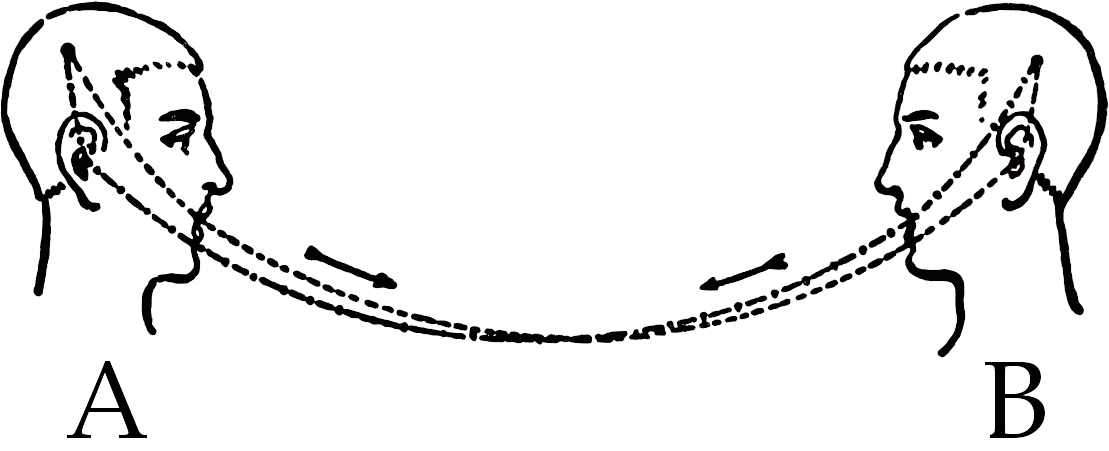
\includegraphics[width=\linewidth]{figures/vol1syntaxe2-img011.png}\medskip\\
    Le point de départ du circuit est dans le cerveau de l’une, par exemple A, où les faits de conscience, que nous appellerons concepts, se trouvent associés aux représentations des signes linguistiques ou images acoustiques servant à leur expression. Supposons qu’un concept donné déclenche dans le cerveau une image acoustique correspondante : c’est un phénomène entièrement \textit{psychique}, suivi à son tour d’un procès \textit{physiologique} : le cerveau transmet aux organes de la phonation une impulsion corrélative à l’image ; puis les ondes sonores se propagent de la bouche de A à l’oreille de B : procès purement \textit{physique}. Ensuite, le circuit se prolonge en B dans un ordre inverse : de l’oreille au cerveau, transmission physiologique de l’image acoustique ; \hi{dans le cerveau association psychique de cette image psychique avec le concept correspondant}. Si B parle à son tour ce nouvel acte suivra — de son cerveau à celui de A — exactement la même marche que le premier et passera par les mêmes phases successives.~» (\citealt{saussure1916cours} : 27--28) [c’est nous qui soulignons]
    \end{quote}

    Saussure insiste, quelques lignes plus loin, sur le fait que l’association entre sens et son qui a lieu dans le cerveau ne se fait pas avec le son lui-même, mais avec une représentation de ce son dans le cerveau, que Saussure nomme l’\hi{image acoustique~}:

    \begin{quote}
    «~[Il faut] distinguer les parties physiques (ondes sonores) des physiologiques (phonation et audition) et psychiques (images verbales et concepts). Il est en effet capital de remarquer que l’image verbale ne se confond pas avec le son lui-même et qu’elle est psychique au même titre que le concept qui lui est associé.~» (\citealt{saussure1916cours} : 28--29)
    \end{quote}

    Leonard \citet[27]{bloomfield1933language}, le père de la linguistique américaine, va dans le même sens :

    \begin{quote}
    «~On produit de nombreuses sortes de bruits vocaux dont on utilise la variété : sous certains types de stimuli, on produit certains sons vocaux et nos compagnons, entendant les mêmes sons, font la réponse appropriée. Pour le dire brièvement, dans la parole humaine, des sons différents ont des sens différents. \hi{Étudier} \hi{la coordination de certains sons avec certains sens,} \hi{c’est} \hi{étudier la langue.}~» [nous soulignons] (Voir les \textit{Citations originales} en fin de chapitre.)
    \end{quote}

    Le fait de considérer que l’objet d’étude de la linguistique est de modéliser la correspondance sens-son décrite par Saussure (et appelée par lui association concept-image acoustique) peut être imputé à Žolkovskij et Mel’čuk qui posent en \citeyear{zolkovski1967semanticeskom} à Moscou les bases de la Théorie Sens-Texte, dont le nom même est tout à fait explicite sur ce point. Dans son cours au Collège de France en \citeyear{melcuk1997vers} intitulé \textit{Vers une linguistique Sens-Texte}, Igor Mel’čuk pose qu’un modèle d’une langue est une correspondance multivoque entre un ensemble de sens et un ensemble de textes, où les textes désignent les images acoustiques des phrases de la langue. Le caractère multivoque est dû au fait qu’un même sens peut être exprimé par différents textes (qui sont alors des «~paraphrases~» les uns des autres) et qu’un texte peut avoir plusieurs sens (c’est-à-dire être sémantiquement ambigu).

    Cette conception de la langue comme une correspondance sens-son est maintenant partagée par la plupart des théories, y compris par la grammaire générative de Noam Chomsky, qui pose, depuis le \textit{programme minimaliste} élaboré dans les années 1990 (voir \cite{chomsky1995minimalist}), qu’un modèle linguistique doit relier sens et sons.
}
\section{Sons et textes}\label{sec:1.1.2}

Il n’est jamais inutile de rappeler que les langues sont avant tout orales (ou gestuelles comme les langues des signes) et que l’écrit n’est qu’une \textstyleTermes{transcription}, nécessairement imparfaite et partielle, des productions orales, même s’il tend à avoir son autonomie et à acquérir sa propre codification. D’après Leonard \citet{bloomfield1933language}, «~L’écrit n’est pas la langue, mais simplement une façon d’enregistrer la langue au moyen de marques visibles. Une langue est la même quel que soit le système d’écriture utilisé pour l’enregistrer, exactement comme une personne est la même quelle que soit la façon dont on prend son image.~» (Nous traduisons en français toutes les citations. Voir les citations originales en fin de chapitre.) La même idée est reprise par H. A. \citet{gleason1955introduction} : «~Une langue écrite est typiquement un reflet, indépendant sous quelques aspects seulement, des langues parlées. En tant qu’image de la parole réelle, elle est inévitablement imparfaite et incomplète. […] La linguistique doit commencer par une étude approfondie de la langue parlée avant d’étudier la langue écrite. C’est vrai pour des langues avec une longue tradition écrite, comme l’anglais, autant que pour les langues de tribus isolées qui n’ont jamais envisagé la possibilité d’une écriture.~» Cent ans avant (dans son ouvrage sur la langue kavi publié en \citeyear{humboldt1836uber}), le philosophe et linguiste Wilhelm von Humboldt écrivait que « la langue, comprise dans son essence réelle, est quelque chose de constant et à la fois, à tout moment, quelque chose de passager. Même sa conservation par l’écriture n’est jamais autre chose qu’un stockage ressemblant à une momie, qui nécessite qu’on cherche à s’imaginer à nouveau le discours vivant.~» Cette primauté de l’oralité est constitutive des sciences du langage et la distingue fondamentalement des lettres et de la philologie (l’étude des textes écrits). Les scientifiques n’en ont néanmoins réellement pris conscience qu’au début du vingtième siècle avec les possibilités nouvelles que donnait l’enregistrement des sons et l’intérêt croissant pour les langues sans tradition écrite et notamment les langues amérindiennes ; la linguistique s’était jusque-là, à l’exception des travaux des missionnaires qui avaient pour mission d’enseigner la Bible dans des langues inconnues, essentiellement développée par l’étude de langues mortes dont on ne conservait que des traces écrites que l’on souhaitait déchiffrer.

Certaines caractéristiques essentielles des langues sont dues au fait que ce sont des modes de communication oraux. La principale de ces caractéristiques est que la communication orale impose une production linéaire : la \textstyleTermes{chaîne parlée} est \hi{unidimensionnelle}. Les sons doivent être produits les uns à la suite des autres. L’écrit n’imposerait pas cela. La communication écrite fait d’ailleurs un grand usage de schémas bidimensionnels souvent complexes et la présentation globale d’un texte écrit (titres, paragraphes, encadrés, etc.) joue un rôle non négligeable. Néanmoins, l’écrit traditionnel, et parce qu’il est au départ une transcription de l’oral, a une organisation linéaire, les mots devant se lire à la suite les uns des autres. On notera qu’aujourd’hui, avec l’internet, les textes contiennent une multitude de liens vers d’autres textes et qu’une production textuelle faite de plusieurs pages web n’est plus totalement linéaire : il a une structure en réseau et on parle alors d’\textstyleTermes{hypertexte}. Cette organisation, qui permet différents parcours du texte, existe déjà en partie dans les écrits traditionnels par la présence de notes ou d’encadrés.

Les langues des signes n’ont pas de contraintes de linéarité, puisque les gestes peuvent se développer dans toutes les dimensions de l’espace et différentes parties du corps être utilisées simultanément (mains, position de la tête, regard, orientation du buste, etc.). Il y a néanmoins une contrainte temporelle dans la communication qui veut qu’il y ait une certaine séquentialité des signes.

Le caractère linéaire de la chaîne parlée est lui-même en partie contourné par l’utilisation de la \textstyleTermes{prosodie~}: les locuteurs ajoutent à la suite des sons distinctifs élémentaires qu’ils produisent — les \textstyleTermes{phonèmes} — de l’information en modulant leur mélodie et en jouant sur l’intensité du signal et la durée des phonèmes. Ceci permet non seulement de communiquer certaines émotions, mais aussi de structurer la chaîne parlée en faisant apparaître des regroupements ou des changements de plan. On retrouve à l’écrit une transcription de la prosodie par la \textstyleTermes{ponctuation} (point, virgule, :, ?, !).  On peut imaginer qu’un langage purement écrit aurait développé un tout autre système et on voit que la ponctuation n’est rien d’autre qu’un marquage partiel et imparfait de la prosodie. On notera que, avec le récent développement du dialogue par écrit, le système de ponctuation s’est enrichi des smileys, émojis et autres émoticônes (\HappySmiley{}, \SadSmiley{}, et plein d’autres).

Nous aurons plusieurs fois l’occasion dans cet ouvrage de montrer que les faits de langue se comprennent bien mieux lorsqu’on se place du côté de l’oral et que notre objet d’étude est d’abord la langue parlée, même si, par commodité, dans un ouvrage écrit, il est souvent plus facile de donner des exemples écrits.

\globe{Langue et variations}{%\label{sec:1.1.3}
     On observe de nombreuses variations entre locuteurs d’une même langue : accent, choix lexicaux, constructions grammaticales, etc. Ces variations sont dues à de multiples facteurs : le degré d’apprentissage de la langue, l’époque à laquelle vit le locuteur, le lieu où il vit, le contexte social dans lequel il s’exprime (la famille, le travail, la radio …), etc. Ainsi l’allemand est pris entre deux langues très proches, le néerlandais et le suisse allemand et on observe un continuum de variétés d’allemand lorsqu’on se rapproche de ces deux zones linguistiques. Pour le français, on observe également des différences de parler suivant les régions, entre le nord et le sud de la France (le système phonologique, notamment, est différent), mais aussi entre la France, la Belgique, la Suisse, le Québec ou les pays francophones d’Afrique. Et à chaque fois, on observe un continuum de parler entre divers extrêmes. Il en va de même pour l’évolution des langues : la limite entre le latin et les langues romanes d’aujourd’hui (italien, espagnol, catalan, français, roumain, corse, etc.) n’est pas une frontière tranchée : le latin a évolué de génération en génération jusqu’à perdre ses désinences casuelles (qu’on ne retrouve dans aucune des langues romanes), puis divers groupes de locuteurs du haut-latin se sont retrouvés isolés au Moyen-Age et ont développés les dialectes que sont nos langues d’aujourd’hui. Le français, ancienne langue d’oïl, a subi l’influence de locuteurs d’origine germanique et la syntaxe de l’ancien français est beaucoup plus proche de celle des langues germaniques d’aujourd’hui (allemand, néerlandais, scandinave) que du latin classique. La situation est identique partout. Si l’on appelle chinois aussi bien le chinois classique que le mandarin actuel, ces langues n’en sont pas moins éloignés que le latin et l’italien. Il existe d’ailleurs aujourd’hui en Chine au moins quatre langues différentes, qui bien que partageant la même écriture, sont plus différentes entre elles que ne le sont les langues romanes entre elles.

    D’une certaine façon, ces variations ne nous intéressent pas : nous décrivons un système unique, celui d’un locuteur donné à un moment donné ou au moins la langue d’un groupe de locuteurs qui communiquent usuellement entre eux. Ce qui nous intéresse avant tout, c’est la cohérence interne de ce système. Néanmoins, les variations possibles de ce système peuvent parfois nous intéresser : elles nous permettent en particulier de comprendre certaines «~bizarreries~» du système qu’on ne saurait expliquer sans prendre en compte le fait qu’il s’agit d’un système en évolution. Par exemple, la non-correspondance entre les unités de forme et les unités de sens (question que nous développerons en long et en large dans la partie 2 consacrée aux \textit{Unités de la langue}) ne peut s’expliquer sans prendre en compte comment de nouveaux termes sont créés par les locuteurs et comment d’autres disparaissent. Il faut d’ailleurs distinguer deux types de changements dans les langues : les changements lexicaux et les changements grammaticaux. Tout locuteur modifie constamment son vocabulaire, acquérant de nouvelles unités lexicales et cessant d’en utiliser certaines. Par contre, il est peu probable qu’une fois l’enfance passée et l’acquisition complète de la grammaire effectuée des changements se produisent dans le système grammatical. Il est plus raisonnable de penser que les changements grammaticaux ont lieu lors du passage de relais d’une génération à l’autre : pour une raison ou une autre, l’apprenant va faire une analyse différente des productions langagières de ses «~instructeurs~» et construire une grammaire différente de la leur. Le cas le plus radical est celui d’un groupe d’apprenants d’une autre langue maternelle qui va projeter sur la langue qu’il apprend des constructions de sa langue maternelle. Les langues romanes et tout particulièrement l’ancien français sont ainsi des formes du latin dont une partie de l’évolution est due à l’assimilation d’apprenants de langue germanique.
}
\section{Sens et intention communicative}\label{sec:1.1.4}

Notre définition de la langue n’est compréhensible que si on s’entend quelque peu sur ce qu’est le sens. Pour cela nous allons partir de la définition que donne Leonard Bloomfield dans \textit{Language}, son ouvrage fondateur de 1933.

Pour Bloomfield, il y a \textstyleTermes{acte de langage} lorsque Jill a faim, qu’elle voit une pomme dans un arbre et qu’au lieu de grimper dans l’arbre la cueillir, elle produit un son avec son larynx, sa langue et ses lèvres et que c’est Jack qui cueille la pomme et la lui apporte. Autrement dit, face à un stimulus S (Jill a faim et voit une pomme), il y a deux voies pour arriver à la réaction R :

\begin{itemize}
\item 
la voie directe S → R, où Jill grimpe dans l’arbre,
\item 
et la voie indirecte S → \begin{tikzpicture}[baseline=(r.base)] \node at (0,0) (r) {r}; \node[right=1em of r] (s) {s}; \draw[dashed,thick] (r) -- (s);\end{tikzpicture} → R, où une réaction linguistique r se substitue à la réaction mécanique de Jill et où le stimulus s qu’elle provoque donne la réaction R chez Jack.
\end{itemize}

Reprenons la citation de Bloomfield, donnée dans l’\encadref{fig:1.1.1} sur \textit{La langue comme correspondance sens-texte}, sous ce nouvel éclairage :

\begin{quote}
    «~On produit de nombreuses sortes de bruit vocaux dont on utilise la variété : sous certains types de stimuli, on produit certains sons vocaux et nos compagnons, entendant les mêmes sons, font la réponse appropriée. Pour le dire brièvement, dans la parole humaine, des sons différents ont des sens différents. Étudier la coordination de certains sons avec certains sens, c’est étudier la langue.~» (\citealt{bloomfield1933language} : 27)
\end{quote}

\noindent Jusque-là, nous sommes parfaitement d’accord. Reste à définir le sens :

\begin{quote}
    «~En produisant une forme linguistique, un locuteur incite son interlocuteur à répondre à une situation ; cette situation et la réponse qu’elle déclenche sont le \textit{sens linguistique} de la forme. Nous supposons que chaque forme linguistique a un sens constant et défini, différent du sens de n’importe quelle autre forme linguistique de la même langue.~» (\citealt{bloomfield1933language} : 165)
\end{quote}

\noindent Là, nous ne sommes plus en accord. Nous pensons qu’il faut absolument séparer la situation du sens linguistique. Dans la même situation, Jill peut produire des énoncés de sens différents comme «~\textit{Pourrais-tu} \textit{me cueillir cette pomme} ?~» ou «~\textit{Apporte-moi cette pomme !~}» ou des énoncés moins coercitifs comme «~\textit{J’ai faim.}~» ou «~ \textit{Regarde cette belle pomme !~}», qui peuvent néanmoins amener la même réaction de Jack. Inversement, dans une tout autre situation, par exemple face à une nature morte dans un musée, Marie peut dire à Pierre «~\textit{Regarde cette belle pomme} !~» et cet énoncé a, pour notre définition du sens, le même sens que l’énoncé «~\textit{Regarde cette belle pomme} !~» de Jill, qui procédait pourtant d’intentions complètement différentes.

Autrement dit, nous distinguons clairement trois objets :

\begin{itemize}
\item le \textstyleTermes{contexte d’énonciation}, c’est-à-dire les caractéristiques extérieures de la situation où est produit l’énoncé : qui parle à qui ? où et quand ? dans quelles circonstances ? etc.
\item les \textstyleTermes{intentions communicatives} du locuteur, c’est-à-dire les buts que se fixe le locuteur, les informations qu’il souhaite communiquer sur tel ou tel objet dans le contexte, etc.
\item le \textstyleTermes{sens linguistique} de l’énoncé, c’est-à-dire, indépendamment du contexte et des intentions du locuteur, le contenu de son message, les éléments de sens qu’il a choisi pour communiquer l’information, désigner tel objet, etc. Le sens linguistique, tel que nous l’envisageons, est très proche du texte, puisqu’il contient déjà les sens des différentes unités du texte.
\end{itemize}

La phase d’élaboration du contenu d’un message, c’est-à-dire le passage d’intentions communicatives dans un contexte donné à un sens linguistique s’appelle la \textstyleTermes{planification} du message. On considère généralement que l’étude de la planification ne relève pas de la linguistique et que cette étape reste relativement indépendante du langage, dans la mesure où toutes les langues permettent d’exprimer à peu près tous les sens (comme le montre l’absence d’obstacles majeurs à la traduction d’une langue à l’autre, sauf lorsqu’il s’agit de concept absent d’une culture à l’autre). Laurence \citet{danlos1987generation}, l’une des pionnières de la génération automatique de textes, propose d’appeler la planification le \textit{Quoi dire}, qu’elle oppose au \textit{Comment le dire}, qui constitue la langue proprement dite.

Nous savons bien sûr que la planification est en partie guidée par le stock lexical que chaque langue propose et nous allons voir un peu plus loin (\sectref{sec:1.1.9}) que la planification joue quand même un rôle dans l’organisation des énoncés et la syntaxe, même si dans cet ouvrage nous étudierons essentiellement le passage du sens au texte. L’étude même des sens linguistiques — la \textstyleTermes{sémantique} — ne sera abordée que dans la mesure où elle interfère avec la syntaxe.

\loupe{Mots et pensée}{%\label{sec:1.1.5}
    La question se pose de savoir si on peut penser sans mots, c’est-à-dire si on peut manipuler des concepts sans les verbaliser, même dans sa tête. Nous pensons que oui. Le bricoleur qui répare son moteur pense à toutes les pièces du moteur qu’il manipule sans avoir nécessairement une idée de comment les appeler et il effectue un grand nombre d’actions bien réfléchies qu’il aurait bien du mal à expliquer en mots. Plus on va vers une pensée abstraite, plus on pourrait penser que les sens doivent se confondre avec les mots. Pourtant, le mathématicien qui fait une démonstration n’a pas toujours les mots pour exprimer les concepts qu’il manipule et une part de son activité est justement d’isoler ces concepts et de leur donner des noms : ensemble, fonction, continuité, etc. Ici il est clair que le concept précède dans la pensée le terme qui lui correspond. Nous faisons l’hypothèse qu’il existe une forme abstraite de pensée sans mots et que la langue est l’ensemble des connaissances qui nous permet d’exprimer cette pensée. Cette hypothèse reste aujourd’hui plus ou moins invérifiable et est controversée. Pour une discussion très lisible de ces idées, voir l’ouvrage de Steven \citet{pinker1997how} sur \textit{Comment fonctionne l’esprit}.
}
\globe{Sens lexicaux et traduction}{%\label{sec:1.1.6}
    Les sens exprimables par des mots simples varient d’une langue à l’autre, ce qui élimine tout espoir de traduction exacte. Par exemple, l’anglais possède une unité lexicale \textsc{melon} qui dénote aussi bien le melon que la pastèque et le français ne possède pas d’équivalent. Le verbe \textsc{esperar} de l’espagnol couvre à la fois les sens ‘espérer’ et ‘attendre’ du français et il existe un continuum entre les deux sens : ‘esperar’ ne sera donc pas ambigu mais «~sous-spécifié~» en ce qui concerne le degré de joie et de certitude qu’a la personne qui «~\textit{espera~}». À l’inverse, le verbe \textsc{aimer} couvre ce que l’anglais exprime avec \textsc{love} et \textsc{like}, car encore une fois, les locuteurs du français considère un continuum entre ces sens. Il existe aussi des sens lexicaux propres à une langue : par exemple, le nom allemand \textsc{schadenfreunde} désigne la joie que procure le dépit mérité des autres et n’a pas d’équivalent en français, bien que le concept puisse être universellement compréhensible. De la même façon, un verbe français comme \textsc{s’accouder} n’aura pas de meilleur équivalent dans beaucoup d’autres langues (par exemple en anglais ou en allemand) qu’une traduction littérale de ‘s’appuyer sur les coudes’.
}
\section{Langue, linguistique et modélisation}\label{sec:1.1.7}

Nous allons définir un certain nombre de termes dont nous aurons besoin et que nous avons déjà commencé à utiliser.

\Definition{\textstyleTermes{locuteur}, \textstyleTermes{sujet parlant}, \textstyleTermes{destinataires}, \textstyleTermes{interlocuteurs}}{Un \textstyleTermes{locuteur} ou \textstyleTermes{sujet parlant} est quelqu’un qui parle, c’est-à-dire quelqu’un qui cherche à communiquer avec d’autres gens en produisant des paroles ou un texte écrit. Il s’adresse à des \textstyleTermes{destinataires} ou \textstyleTermes{interlocuteurs}.}

\Definition{\textstyleTermes{langue}}
{Une \textstyleTermes{langue} est un système de signes conventionnels partagés par un certain nombre de personnes et qui leur permet de communiquer entre elles. Ces signes s’assemblent pour former des mots, des phrases et des discours. Une langue est à la fois un \hi{objet individuel} — c’est l’ensemble des connaissances stockées dans notre cerveau qui nous permettent de parler (dans cette langue) — et un \hi{objet collectif} et \hi{social}, puisque ces connaissances sont partagées par un certain nombre de personnes, qui sont les locuteurs de cette langue.}

\Definition{\textstyleTermes{faculté langagière}, \textstyleTermes{la langue}}
{La \textstyleTermes{faculté langagière} est l’aptitude que nous avons à apprendre et utiliser les langues. Le cerveau est l’organe de la faculté langagière (avec le système phonatoire que le cerveau commande pour produire des sons). Lorsqu’on parle de \textstyleTermes{la langue}, et non plus d’une langue particulière, on fait généralement référence à la faculté langagière et ce qu’elle va imposer comme traits communs à l’ensemble des langues possibles.}

\Definition{\textstyleTermes{linguistique}}
{La \textstyleTermes{linguistique} est la science qui étudie les langues du monde. Comme beaucoup de scientifiques, nous considérons que la linguistique inclut l’étude de la faculté langagière, c’est-à-dire l’étude de la production langagière et de l’apprentissage d’une langue par l’enfant. La linguistique est alors quasiment une branche de la psychologie.}

La linguistique produit des \textstyleTermes{modèles des} \textstyleTermes{langues} et de la faculté langagière. Ces modèles doivent être capables de simuler un \textstyleTermes{acte de langage}, c’est-à-dire la façon dont un locuteur produit un texte à partir d’un sens qu’il veut exprimer et la façon dont son interlocuteur reconstruit un sens à partir de ce texte.

Tout modèle se situe dans un \textstyleTermes{cadre théorique}. Décider que la langue est une correspondance est un choix théorique. Décider ce qui est mis en correspondance par la langue, c’est-à-dire ce que sont la représentation sémantique et le texte relève aussi de choix théoriques. C’est le cadre théorique qui caractérise notamment l’objet d’étude. Pour reprendre une formule de \citet{saussure1916cours} devenue fameuse, «~Bien loin que l’objet précède le point de vue, on dirait que c’est le point de vue qui crée l’objet.~».

\loupe{Langue et parole, compétence et performance}{%\label{sec:1.1.8}
    Saussure oppose deux notions fondamentales qu’il nomme \textstyleTermes{langue} et \textstyleTermes{parole~}:

    \begin{quote}
    «~Entre tous les individus ainsi reliés par le langage, il s’établira une sorte de moyenne : tous reproduiront, — non exactement, mais approximativement — les mêmes signes unis aux mêmes concepts. […]

    La {langue} n’est pas une fonction du sujet parlant, elle est le produit que l’individu enregistre passivement. […] Elle est la partie sociale du langage, extérieure à l’individu, qui à lui seul ne peut ni la créer ni la modifier ; elle n’existe qu’en vertu d’une sorte de contrat passé entre les membres de la communauté. […]

    La {parole} est au contraire un acte individuel de volonté et d’intelligence, dans lequel il convient de distinguer :

    1° les combinaisons par lesquelles le sujet parlant utilise le code de la langue en vue d’exprimer sa pensée personnelle ;

    2° le mécanisme psycho-physique qui lui permet d’extérioriser ces combinaisons.~»\\
    (\citealt{saussure1916cours} : 29-31)
    \end{quote}

    La parole, au sens de Saussure, couvre deux notions qu’il convient de séparer. Nous préférons parler de \textstyleTermes{productions langagières} pour la première notion, c’est-à-dire les énoncés réellement produits par des sujets parlants, tandis qu’on préférera appeler la deuxième notion la \textstyleTermes{faculté langagière}. Alors que la parole est un objet individuel, la \textstyleTermes{langue} est un objet social par excellence, mais c’est aussi la trace qu’a imprimée cet objet dans le cerveau de chacun de nous, objet collectif, donc, qui n’existe que par la somme de ses traces individuelles.

    L’opposition entre compétence et performance proposée par \citet{chomsky1965aspects} nous renvoie à l’opposition entre langue et parole, mais il convient de les distinguer : la compétence ne se confond pas avec la langue, ni la performance avec la parole. La \textstyleTermes{compétence} désigne notre compétence passive à savoir utiliser la langue, mais aussi à l’acquérir. Elle se divise en une compétence innée, qui peut se confondre avec la faculté langagière, et une compétence acquise, qui peut se confondre avec la langue en tant que trace individuelle d’une langue dans notre cerveau.

    La \textstyleTermes{performance} est l’usage proprement dit de la langue. La \textstyleTermes{parole} est le produit de la compétence et de la performance : nous avons la compétence de produire des énoncés supposément parfaits, mais divers facteurs (notre état émotionnel, des éléments qui vont nous distraire, la recherche d’un message approprié, etc.) vont faire que notre énoncé ne sera pas aussi parfait qu’il aurait pu l’être. Ceux qui veulent décrire la langue, comme nous, vont essayer de séparer ce qui relève d’un \textstyleTermes{manque de compétence} de ce qui relève d’une \textstyleTermes{erreur de performance}. La chose est loin d’être évidente, notamment lorsqu’on touche aux \textstyleTermes{limitations mémorielles}. Par exemple, Chomsky a beaucoup insisté sur le caractère \textstyleTermes{récursif} de la langue : une proposition peut contenir une proposition subordonnée (\textit{La personne} [\textit{que le chien a mordu}] \textit{est à l’hôpital}) et un tel enchâssement peut être itéré (\textit{La personne} [\textit{que le chien} [\textit{auquel le garçon a donné un os}] \textit{a mordu}] \textit{est à l’hôpital}). Mais cette dernière phrase est difficilement compréhensible et une insertion de plus dépasse nos capacités d’analyse en situation de communication ordinaire (\textit{La personne que le chien auquel le garçon qui habite au coin de la rue a donné un os a mordu est à l’hôpital}). Défaut de compétence ou de performance ? (Voir Exercice 3.)
}
\section{La planification}\label{sec:1.1.9}

Nous voudrions montrer ici que la planification (voir définition dans la \sectref{sec:1.1.4} sur \textit{Sens et intention communicative}) peut avoir des incidences non négligeables sur la nature du texte produit et que dans l’absolu il faut l’inclure dans notre objet d’étude. En particulier, on ne peut pas en général considérer que le locuteur construit le contenu de son message avant de le transformer en un énoncé, c’est-à-dire qu’il planifie complètement avant de produire un énoncé. Les choses ne se passent généralement pas comme ça et le locuteur élabore le contenu de son message au fur et à mesure de l’énonciation. Les productions orales présentent en particulier de nombreux indices de la planification en cours. (C’est moins net à l’écrit, puisque le scripteur à la possibilité de revenir en arrière pour corriger sa production.) Comme le dit Claire \citet[17]{blanche-benveniste1990francais}, «~Lorsque nous produisons des discours non préparés, nous les composons au fur et à mesure de leur production, en laissant des traces de cette production. […] L’étude de ces traces est en elle-même un sujet d’observations ; on y voit la production de langage en train de se faire. […] Une observation attentive permet de voir comment nous procédons, quelles unités nous utilisons pour faire avancer nos discours, quelles tenues en mémoire nous avons, à la fois pour les morceaux déjà énoncés et pour ceux que nous projetons d’énoncer. On peut ainsi observer comment se fait la mise au point des syntagmes, la recherche des «~bonnes dénominations~», et le travail constant d’évaluation que nous faisons sur nos propres discours.~»

Nous allons montrer trois phénomènes qui illustrent l’influence de la planification sur la structure de l’énoncé. Les exemples qui suivent sont des retranscriptions fidèles de productions orales attestées ; dans ces transcriptions figurent absolument tous les mots prononcés par le locuteur, y compris les bribes et répétitions dues aux hésitations du locuteur.

Les premiers indices de la planification en cours sont les nombreuses amorces que le locuteur fait et auxquelles il renonce momentanément ou définitivement. Dans l’exemple suivant, la locutrice semble ne pas trouver tout de suite la bonne formulation ; elle hésite et répété \textit{les} pour se donner du temps, amorce la production de \textit{les capitales}, mais s’y prend quand même à deux fois pour finalement proposer une reformulation par \textit{les grandes villes} :

\ea\itshape et je voulais pas aller à Addis Abeba puisque \textbf{les les les les c-} \textbf{les capitales les grandes villes} ne me disaient rien du tout\z

À chaque fois, on obtient une \textstyleTermes{bribe}, c’est-à-dire un segment inachevé qui est ensuite corrigé par le locuteur. La disposition suivante du texte, dite \textstyleTermes{analyse en grille}, permet de mettre en évidence l’\textstyleTermes{entassement} (voir le \chapref{sec:5.5}) dans la même position syntaxique de la bribe et du segment qui vient la remplacer :

\ea \begin{tabularx}{\linewidth}[t]{@{}l|>{\hangindent=1em}Q@{}}
et je voulais pas aller à AA puisque  & \textbf{les}\\
                                      & les\\
                                      & les\\
                                      & les c-\\
                                      & les capitales\\
                                      & \textbf{les grandes villes} ne me disaient rien du tout
    \end{tabularx}
\z

Plus étonnant est le phénomène de la \textstyleTermes{greffe} bien étudié par José Deulofeu (voir la partie 6). L’exemple suivant en fourni deux :

\ea
on avait critiqué le le journal de je crois que c’était le Provençal on l’avait critiqué par rapport à ou le Méridional par rapport à la mort de comment il s’appelle … pas Coluche l’autre

%%[Warning: Draw object ignored]
\z

À deux reprises, ici, le locuteur ne trouve pas le nom qu’il cherche et il vient greffer un énoncé qui pourrait fonctionner comme un énoncé autonome et qui est ici inséré dans l’énoncé principal dont il assure la complétion. Nous reprenons le texte précédent en le disposant selon les principes de l’analyse en grille et en indiquant les greffes en gras.

\ea \begin{tabular}[t]{@{}|l|l|l@{}}
on avait critiqué & \multicolumn{2}{l}{le}\\
                  & \multicolumn{2}{l}{le journal de}\\
                  & je crois que c’était  &  le Provençal\\
\multicolumn{1}{@{}|l}{} & \multicolumn{1}{l|}{} & \multicolumn{1}{l@{}}{}\\
on l’avait critiqué &  par rapport à & \\
\multicolumn{1}{@{}l|}{} &                & ou le Méridional\\
\multicolumn{1}{@{}l|}{} & \multicolumn{1}{l}{} & \multicolumn{1}{l@{}}{}\\
\multicolumn{1}{@{}l|}{} & par rapport à la mort de  &  \textbf{comment il s’appelle}\\
\multicolumn{2}{@{}c|}{} & pas Coluche\\
\multicolumn{2}{@{}c|}{} & l’autre             
\end{tabular}\todo[inline]{please check \& confirm}
\z

On notera que la première greffe s’entrelace avec l’énoncé principal, ce qui semble montrer que le locuteur poursuit en parallèle la planification de son énoncé principal et de la greffe. On voit à nouveau ici un fonctionnement par entassement de segments similaires ou identiques (\textit{on avait critiqué le journal - on l’avait critiqué, par rapport à - par rapport à}).

Un dernier phénomène illustre bien le fait que la planification a lieu en même temps que l’énonciation : les parenthèses. On appelle \textstyleTermes{parenthèse} tout énoncé qui vient s’insérer dans l’énoncé principal et qui est marqué par un changement de registre (une modification de l’intonation) qui le détache nettement de l’énoncé principal. Dans le texte suivant, nous avons indiqué les parenthèses entre parenthèses et nous avons directement disposé le texte en grille :

\ea donc pour essayer un petit peu de sortir cette personne de la misère (car c’est vraiment un petit peu semblable aux Misérables de Victor-Hugo) nous essayons tant bien que mal de lui faire comprendre que \textbf{sa cabane}\\
\begin{tabular}[t]{@{}|p{1cm}ll@{}}
    & \multicolumn{2}{|l}{dans quelques années (entre parenthèses, elle a 79 ans)}\\
    & \multicolumn{1}{|l}{quand elle aura} & \multicolumn{1}{|l}{des difficultés (ce qu’on espère pas)}\\
    & \multicolumn{1}{|l}{} & \multicolumn{1}{|>{\hangindent=1em}p{.55\textwidth}}{des difficultés à se déplacer ou à évoluer (c’est-à-dire qu’il y a énormément d’escaliers à monter pour arriver à sa cabane)}\\
    & \multicolumn{1}{|l}{donc le jour} & \multicolumn{1}{|l}{où elle ne pourra plus se déplacer}\\
    & \multicolumn{1}{|l}{} & \multicolumn{1}{|>{\hangindent=1em}p{.55\textwidth}}{ou qu’elle sera malade un petit peu plus sévèrement,}\\
    \multicolumn{3}{|>{\hangindent=1em}p{.85\textwidth}}{on essaye de lui faire comprendre qu’elle ne pourra plus vivre dans cette cabane}
\end{tabular}\todo[inline]{Kindly review \& comment}
\z

On peut résumer le contenu de ce texte ainsi : comme cette personne a 79 ans et qu’il y a énormément d’escaliers pour arriver à sa misérable cabane, il faut lui faire comprendre qu’elle ne pourra plus y vivre dans quelques années. On voit que deux informations essentielles (‘elle a 79 ans’ et ‘il y a énormément d’escaliers’) ont été ajoutées à la volée, ce qui a finalement obligé le locuteur à abandonner sa première proposition (\textbf{\textit{sa cabane}}, en gras dans le texte, est le sujet d’un verbe originalement planifié qui ne vient jamais) et à reprendre par une proposition équivalente (\textit{nous essayons tant bien que mal de lui faire comprendre que sa cabane} → \textit{on essaye de lui faire comprendre qu’elle ne pourra plus vivre dans cette cabane}). Il est probable qu’à la première lecture (qui aurait normalement dû être une écoute) de ce texte, vous ne vous êtes pas rendu compte que la première proposition avait été laissée inachevée : ceci montre le caractère très naturel de telles constructions et le fait que le destinataire est habitué à «~corriger~» les «~erreurs~» dues à la planification.

Les linguistes considèrent généralement que la planification est hors de leur objet d’étude et que la langue constitue uniquement le passage du contenu du message, c’est-à-dire le sens, à un énoncé. Les exemples précédents montrent que la planification, ou plutôt les problèmes de planification, laisse de nombreuses traces en surface et qu’il est donc difficile d’en faire abstraction, surtout si on étudie les productions orales. À l’écrit, par contre, les défauts de planification sont gommés par les passages successifs du rédacteur et la possibilité d’interrompre la rédaction pendant la planification. Ceci est encore une raison de préférer l’étude de l’oral à celle de l’écrit, car on trouve à l’oral davantage d’indices de la façon dont les locuteurs «~travaillent~», alors les corrections successives sont invisibles à l’écrit.

\section{Corpus et introspection}\label{sec:1.1.10}

Il existe deux moyens d’obtenir des faits de langue pour le linguiste. Le premier est de collecter des textes déjà produits. Un ensemble de textes est appelé un \textstyleTermes{corpus}. Le plus grand corpus disponible est le web et les moteurs de recherche constituent un assez bon moyen de récolter les données que l’on cherche, même s’il faut savoir trier ces données selon le type de page~(site d’information, blog, forum, chat, etc.) et le type d’auteur (locuteur natif, génération automatique, traduction automatique, etc.). Il existe des corpus plus spécialisés, comme les bibliothèques numériques d’ouvrages classiques, les archives des grands journaux, les encyclopédies en ligne ou les revues scientifiques. Les linguistes constituent des corpus pour leur besoin, notamment des corpus de productions orales dont les textes sont minutieusement retranscrits à l’écrit (nous en avons donné des exemples dans la section précédente). Certains de ces corpus concernent des populations particulières : enfants en phase d’acquisition, apprenants d’une seconde langue, aphasiques, etc. Tous ces paramètres constituent le \textstyleTermes{genre} de la production textuelle. Un bon corpus doit comporter ce type d’informations, qu’on appelle les \textstyleTermes{métadonnées}, c’est-à-dire les données qui concernent le corpus et se trouvent à côté des données proprement dites. En plus des métadonnées, certains corpus sont agrémentés d’annotations diverses permettant une meilleure étude des structures des énoncés. On trouve également des corpus alignés de différentes langues (qu’on appelle corpus multilingues ou bitextes) très utiles pour développer des modèles pour la traduction.

Le deuxième moyen d’étude est \textstyleTermes{l’introspection}. Il s’agit de construire artificielle\-ment des énoncés et d’en faire juger l’\textstyleTermes{acceptabilité} par des locuteurs natifs. Ce moyen permet de tester toutes les variantes imaginables d’un phénomène et surtout de vérifier les limites d’un phénomène en produisant des énoncés jugés inacceptables. Une autre raison qui peut justifier le recours à l’introspection est que, sur corpus, on rencontre beaucoup d’erreurs de performance, qui font que certains énoncés seraient jugés inacceptables même par ceux qui les ont produits. Il est donc nécessaire de garder un esprit critique et de savoir filtrer les résultats.

Un énoncé produit dans des conditions normales de production est dit \textstyleTermes{attesté}, par opposition à un énoncé \textstyleTermes{construit} par le linguiste. Même si nous ne rejetons pas l’introspection et l’appel au jugement des locuteurs, nous considérons que l’étude des corpus restent le meilleur moyen d’accéder aux données et d’éviter de passer à côté de phénomènes importants.

\section{Acceptabilité}\label{sec:1.1.11}
\subsection{Degrés d'acceptabilite}
Parmi toutes les phrases bizarres qu’un linguiste rencontre ou construit, il est souvent difficile de classer les phrases en bonnes et mauvaises. On constate plutôt une gradation de «~qualité~» qu’un jugement binaire en bon et mauvais.

Considérons les énoncés construits suivants :

\ea
\ea \itshape C’est un film que je sais que tu n’hésiteras pas une seconde à regarder.
\ex \itshape C’est un film que je me demande quand tu regarderas.
\ex \itshape C’est un film que je ne sais pas si tu accepteras que je regarde.
\ex \itshape C’est un film que je me demande jusqu’où tu es prêt à regarder.
\ex \itshape C’est un film que je dormais quand tu regardais.
\z
\z

On ressent facilement que la phrase (A) est meilleure que la phrase (B), qui elle-même est meilleure que (C). On constate que la phrase (E) est clairement inacceptable, tandis qu’on peut se demander si (D) l’est ou pas. Il est d’usage de noter l’\textstyleTermes{acceptabilité} des énoncés par des symboles allant de l’absence de symbole signifiant l’acceptabilité au symbole~* signifiant l’inacceptabilité, en passant par les symboles ? (léger doute), ?? (doute sérieux) et ?* (inacceptabilité probable). Pour nos exemples, nous aurions donc :

\ea
\judgewidth{\textsuperscript{?}*}
\ea[]{\itshape C’est un film que je sais que tu n’hésiteras pas une seconde à regarder.}
\ex[\textsuperscript{?}]{\itshape C’est un film que je me demande quand tu regarderas.}
\ex[\textsuperscript{??}]{\itshape C’est un film que je ne sais pas si tu accepteras que je regarde.}
\ex[\textsuperscript{?}*]{\itshape C’est un film que je me demande jusqu’où tu es prêt à regarder.}
\ex[*]{\itshape C’est un film que je dormais quand tu regardais.}
\z
\z

Les marques d’acceptabilité ne sont pas absolues et doivent plutôt être interprétées comme relatives (c’est-à-dire qu’un énoncé marqué ?? est plus acceptable qu’un énoncé marqué ?*).

\subsection{Acceptabilité et grammaticalité}

Lorsqu’on étudie la syntaxe, il est important de faire abstraction des problèmes qui viennent de la sémantique. Comparons les deux énoncés suivants :

\ea
\ea\itshape D’élégants chevaux blancs courent librement.
\ex\itshape D’incolores idées vertes dorment furieusement.
\z
\z

Évidemment, l’énoncé \REF{ex:key:2}, traduit d’un célèbre exemple de Noam Chomsky (Colorless green ideas sleep furiously), est plus que bizarre et il est difficile de trouver un contexte, autre que poétique, où cet énoncé aurait un sens approprié. Pourtant d’un strict point de vue syntaxique, l’énoncé \REF{ex:key:2} est identique à \REF{ex:key:1} et peut être jugé comme tout à fait \textstyleTermes{grammatical}.

Voici un autre exemple (attesté) d’une phrase grammaticale, mais incompréhensible, car trop complexe et appartenant à un langage de spécialité dont le vocabulaire nous est inhabituel :

\ea\itshape
À mon avis, à l’exception de l’effet des éventuels redressements que j’aurais pu juger nécessaires si j’avais pu m’assurer de l’intégralité des produits dont il est question au paragraphe précédent, ces états financiers présentent fidèlement, à tous égards importants, la situation financière de la société au 31 décembre 1996 ainsi que les résultats de son exploitation et l’évolution de sa situation financière pour la période de douze mois terminée à cette date selon les principes comptables généralement reconnus.
\z

Lorsqu’un énoncé est grammatical, mais jugé \textstyleTermes{inapproprié}, nous utilisons le symbole \#. Ainsi en réponse à la question «~\textit{Qui a mangé les framboises~}?~», la réponse suivante sera jugée inappropriée :

\ea
\textsuperscript{\#}{\itshape C’est les framboises que Pierre a mangées}.
\z

Autre exemple : quand on parle des expressions figées, on peut relever que $⌜$\textsc{briser} \textsc{la} \textsc{glace}$⌝$ (au sens de ‘dissiper la gêne’) se passive, mais pas $⌜$\textsc{perdre} \textsc{les} \textsc{pédales}$⌝$ (au sens de ‘perdre le contrôle de soi-même’)~:

\ea
 \ea[]{\itshape Marie a brisé la glace.}
 \ex[]{\itshape La glace a été brisée par Marie}
 \ex[]{\itshape Marie a perdu les pédales.}
 \ex[\textsuperscript{\#}]{\itshape Les pédales ont été perdues par Marie.}
\z
\z

Cette dernière phrase est grammaticale, mais elle a perdu le sens figé (la seule lecture possible est littérale : on parle vraiment de pédales et d’une perte) et elle n’a donc plus le sens approprié.

Enfin, lorsqu’une combinaison morphologique est jugée inappropriée, car absente du stock lexical actuel, nous utilisons le symbole ° : °\textit{tournement,} °\textit{bravitude}, °\textit{aspire-poussière}, °\textit{loup-chien}, etc.

\section{Parler et comprendre}\label{sec:1.1.12}

Si les textes (oraux ou écrits) sont le principal moyen d’accès à la langue, il ne faut pas oublier que la description des textes n’est pas notre finalité. Un texte est une production langagière et c’est bien la production du texte qui, derrière le texte, nous intéresse.

Une langue est une correspondance entre sens et textes et donc modéliser la langue ce n’est pas seulement modéliser les textes de cette langue, mais modéliser la correspondance entre sens et textes. Or il y a deux façons d’effectuer cette correspondance : soit on passe du sens au texte, c’est-à-dire qu’on parle, soit on passe du texte au sens et l’on est dans une situation d’analyse et de décodage du texte.

La plupart des études partent des textes et donc modélisent la langue dans le sens de l’\textstyleTermes{analyse}. Nous pensons, à la suite d’Igor Mel’čuk, qu’il est préférable d’étudier la production et de travailler dans le sens de la \textstyleTermes{synthèse} (on parle encore de \textstyleTermes{génération de textes} quand la production est automatisée). Ceci peut paraître parfois délicat, car pour étudier la production, il faut partir d’une intention communicative et donc commencer par construire un sens. Mais c’est le seul moyen de comprendre quelles sont les contraintes qui s’exercent sur le locuteur et modèlent la langue. Nous allons illustrer notre propos en étudiant un exemple de production dans le chapitre suivant.

\exercices{%\label{sec:1.1.13}
    \exercice{1} S’intéresse-t-on aux variations individuelles entre locuteurs d’une même langue ?

    \exercice{2} Le symbole \textsuperscript{?}* veut-il dire qu’on ne croit pas que la phrase est agrammaticale ?

    \exercice{3} Nous avons terminé l’\encadref{fig:1.1.8} en nous demandant si le fait que la phrase \textit{La personne que le chien auquel le garçon qui habite au coin de la rue a donné un os a mordu est à l’hôpital} était incompréhensible mettait en évidence un problème de compétence ou de performance. Quel élément de réponse peut-on apporter ?

    \exercice{4} Quel phénomène intéressant observe-t-on dans les énoncés suivants du point de vue de la planification ?
    
    \begin{enumerate}[label=(\arabic*)]
    \item mais voilà ça c’est une sorte de mélange très très très étrange et qui moi me je sais pas pourquoi me renverse littéralement

    \item vous allez passer devant la poste qui sera à votre droite et un peu plus loin euh je sais pas à quel niveau c’est exactement Habitat et euh la Chambre de de Commerce à votre gauche
    \end{enumerate}

 \exercice{5} La société humaine repose sur la croyance. Cette idée est très bien développée dans \textit{Sapiens - Une brève histoire de l’humanité} de Yuval Noah \citet{harari2014sapiens}. La question dépasse très largement la croyance religieuse. Notre société fonctionne car nous, humains, croyons en un même système de lois, nous croyons dans les valeurs de notre société, comme l’éducation ou la solidarité, nous croyons en la valeur de l’argent, alors même qu’il peut s’agir d’un simple bout de papier imprimé ou d’un nombre dans la mémoire d’un ordinateur de notre banque. En quoi la notion de croyance (ainsi définie) concerne la linguistique et la langue ?
}
\lecturesadditionnelles{%\label{sec:1.1.14}

     Les ouvrages de Ferdinand de \citet{saussure1916cours} et de Leonard \citet{bloomfield1933language} sont des monuments de la linguistique, dont la lecture reste toujours incontournable. Le livre de Wilhelm von Humboldt de \citeyear{humboldt1836uber} est un ouvrage précurseur, mais difficile à lire aujourd’hui. La lecture des ouvrages de Claire Blanche-Benveniste est une excellente plongée dans les données véritablement attestées et ce qu’elles révèlent sur la syntaxe du français parlé et la langue en général. Le livre de Henry A. \citet{gleason1955introduction} est une introduction très pédagogique aux bases de la linguistique et de la syntaxe, qui a étonnamment peu vieillie. Le cours donné par Igor Mel’čuk au collège de France complétera les ouvrages de ce linguiste déjà mentionné dans l’\textit{Avant Propos}. Les lecteurs intéressés par l’histoire des sciences pourront consulter les premiers travaux sur la Théorie Sens-Texte de Žolkovskij et Mel’čuk de \citeyear{zolkovski1967semanticeskom}, traduits en français en 1970. Les bases de la génération automatique de textes sont développées dans l’ouvrage fondateur de Laurence \citet{danlos1987generation}. Nous avons également mentionné les ouvrages de Steven \citet{pinker1997how} et de Yuval Noah \citet{harari2014sapiens}, qui ne concernent pas directement notre sujet, mais s’inscrivent dans une approche scientifique des sciences humaines que nous suivons.

    \FurtherReading{1-1}
}
\citations{%\label{sec:1.1.15}
    {\bfseries
    Citations de la \sectref{sec:1.1.1}.
    }


    {\citet[27]{bloomfield1933language}} :
    \begin{quote}
    ~Man utters many kinds of vocal noise and make use of the variety: under certain types of stimuli he produces certain vocal sounds and his fellows, hearing the same sounds, make the appropriate response. To put it briefly, in human speech, different sounds have different meanings. To study this co-ordination of certain sounds with certain meanings is to study language.
    \end{quote}

    {\bfseries
    Citations de la \sectref{sec:1.1.2}.
    }
    {\citet{bloomfield1933language}} : 

    \begin{quote}
    Writing is not language, but merely a way of recording language by means of visible marks. […] A language is the same no matter what system of writing may be used to record it, just as a person is the same no matter how you take is picture.
    \end{quote}

    {\citet{gleason1955introduction}} :

    \begin{quote}

    A written language is typically a reflection, independent in only limited ways, of spoken languages. As a picture of actual speech, it is inevitably imperfect and incomplete. […] Linguistics must start with thorough investigation of spoken language before it proceeds to study written language. This is true for language with long histories of written literature, such as English, no less than those of isolated tribes which have never known of the possibility of writing.
    \end{quote}

    {\citet{humboldt1836uber}} :

    \begin{quote}
    Die Sprache in ihrem wirklichen Wesen aufgefasst ist etwas beständig und in jedem Augenblicke Vorübergehendes. Selbst ihre Erhaltung durch die Schrift ist immer nur eine unvollständige mumienartige Aufbewahrung die es doch erst wieder bedarf dass man dabei den lebendigen Vortrag zu versinnlichen sucht.
    \end{quote}
    \textbf{Citations de la section \ref{sec:1.1.4}.}

    {\citet[165]{bloomfield1933language}} :

    \begin{quote}
    By uttering a linguistic form, a speaker prompts his bearers to respond to a situation; this situation and the response to it are the linguistic meaning of the form. We assume that each linguistic form has a constant and defining meaning, different from the meaning of any other linguistic form in the same language.
    \end{quote}
}
\corrections{%\label{sec:1.1.16}
    \corrigé{1} Certains linguistes s’intéressent beaucoup aux variations individuelles, notamment les chercheurs en acquisition des langues ou en socio-linguistique. Mais dans cet ouvrage, nous ne nous y intéresserons pas vraiment : nous voulons modéliser un système linguistique particulier et pas les variations entre deux systèmes. Qui plus est, nous privilégierons dans notre étude les règles qui sont communes au plus grand nombre de locuteurs. Et en même temps, nous savons qu’il existe des variations et nous voulons que le système que nous proposons soit capable de les saisir.

    \corrigé{2} Non, il signifie qu’on n’est pas complètement sûr que la phrase soit grammaticale. Voir \sectref{sec:1.1.11}.

    \corrigé{3} Précisons pour commencer que le problème ne se situe pas du côté de la compréhension. Le problème n’est pas que cette phrase ne sera pas comprise, le problème est qu’elle ne pourra pas être produite par un locuteur dans une situation normale de communication. Pour la produire, nous avons fait un travail de linguiste et pas de locuteur ordinaire, en appliquant des insertions successives de relatives. À partir de là, nous considérons que les locuteurs n’ont pas la compétence de produire de tels énoncés et que cela n’a rien à voir avec la performance. Mais on peut aussi estimer (comme Noam Chomsky) que cette limitation n’est pas à proprement parler une propriété de la langue et qu’elle relève d’une modélisation des capacités cognitives en général. Si le modèle linguistique est combiné avec un tel modèle, on peut ne pas tenir compte des limitations mémorielles dans la modélisation des langues. Quoi qu’il en soit, il faut, à notre avis, les prendre en compte quelque part dans un modèle de la compétence.

    \corrigé{4} Ces deux énoncés présentent une parenthèse (\textit{je sais pas pourquoi} dans le premier et \textit{je sais pas à quel niveau c’est exactement} dans le second). Il s’agit d’un énoncé syntaxiquement indépendant à l’intérieur d’un autre énoncé. Cela illustre la capacité du locuteur à commenter ce qu’il dit (comme si quelqu’un d’autre venait interrompre son propos) sans pour autant perdre le fil de ce qu’il dit.

    \corrigé{5} Toute langue repose sur un système de conventions que les locuteurs doivent accepter. De la même façon que nous acceptons qu’un billet de 20€ a pour tous nos condisciples deux fois plus de valeur qu’un billet de 10€, nous acceptons que le texte \textit{un chien} désignera bien un chien pour nos condisciples. L’apprentissage d’une langue repose donc sur la croyance que les conventions linguistiques seront acceptées par nos condisciples. Pour qu’une langue existe, il faut qu’un groupe d’humains accepte de croire au système de conventions qu’elle suppose. On peut citer \citet[31]{saussure1916cours} : «~[La langue] est la partie sociale du langage, extérieure à l’individu, qui à lui seul ne peut ni la créer ni la modifier ; elle n’existe qu’en vertu d’une sorte de contrat passé entre les membre de la communauté.~» On considère généralement qu’il existe deux types d’entités : les entités objectives, qui appartiennent au monde réel, et les entités subjectives, que je crée dans mon cerveau. Il existe en fait un troisième type d’entités, qu’Harari appelle les \textstyleTermes{entités inter-subjectives}, et qui n’existent qu’à travers un accord entre les individus d’une communauté : Zeus, l’euro (la monnaie), la France, Google (la société) ou encore la langue française. Toutes ces choses n’existent que parce que les humains pensent qu’elles existent. Si les humains disparaissent, ces choses disparaîtront avec eux.
}

\chapter{\gkchapter{Produire un énoncé}{La syntaxe mise en évidence par un exemple}}\label{sec:1.2}

\section{Analyse et synthèse}\label{sec:1.2.0}

Ce chapitre est entièrement consacré à l’étude de la production d’un énoncé ou plus exactement à la production d’une famille d’énoncés concurrents exprimant plus ou moins le même sens. Il est habituel de commencer l’étude d’une langue en analysant les textes (éventuellement oraux) produits dans cette langue. L’étude procède alors dans le sens de l’\textstyleTermes{analyse}, c’est-à-dire du texte vers le sens. Nous pensons, à la suite de Lucien Tesnière et d’Igor Mel’čuk, qu’il est préférable d’étudier la langue dans le sens de la \textstyleTermes{synthèse}, c’est-à-dire du sens vers le texte.

Pour comprendre le fonctionnement de la langue, il est donc nécessaire d’étudier la façon dont un énoncé est produit par un locuteur et les opérations qui conduisent à la production de cet énoncé. Nous mettrons en évidence un ensemble de contraintes auxquelles doit obéir le locuteur lors de l’énonciation et qui constitue la grammaire de la langue. Parmi ces contraintes, nous verrons que la langue nous impose une structuration hiérarchique qui constitue le cœur de la syntaxe.

\loupe[sec:1.2.1]{Les observables : textes et sens}{
    Un modèle se construit à partir d’\textstyleTermes{observables}, puisqu’il modélise le fonctionnement de quelque chose de réel, que l’on peut observer. Néanmoins, un modèle est amené à faire des hypothèses sur la façon dont ces observables sont produits et à construire ainsi un certain nombre d’objets qui ne sont pas observables.

    Pour ce qui est de la langue, deux choses sont réellement observables : les textes et les sens. Pour les textes, c’est assez évident, même si la question de savoir quelle est la représentation d’un texte dans notre cerveau reste un problème. Pour les sens, c’est plus complexe : on ne peut pas observer le sens en tant que tel, mais on peut s’assurer qu’un texte est compréhensible et qu’il est compris. L’un des outils d’observation est la paraphrase : on peut demander à un locuteur de reformuler un texte ou lui demander si deux textes ont le même sens. On peut ainsi considérer, à la suite d’Igor \citet[52]{melcuk1988dependency}, que «~avoir le même sens~» est un observable et \hi{définir le sens} comme un invariant de paraphrases, c’est-à-dire comme ce qui est commun à tous les textes qui ont le même sens.

    Nous faisons l’hypothèse qu’il y a entre le sens et le texte un niveau d’organisation syntaxique. Cette organisation n’est pas directement observable. Dans la suite, nous serons amenés à construire un grand nombre d’objets linguistiques et notamment des représentations syntaxiques. Il s’agit de \hi{constructions théoriques} et de rien d’autre. On ne prouve leur «~existence~» qu’à l’intérieur d’une théorie. Elles existent dans le modèle, mais cela ne prouve pas qu’elles existent dans l’objet réel que nous modélisons. On ne peut pas réfuter directement leur existence. On ne peut que réfuter l’adéquation du modèle avec l’objet modélisé. Néanmoins, si le modèle est adéquat et suffisamment économique, alors les objets construits par le modèle acquièrent une part de réalité, deviennent plus tangibles.
}
\section{Partir d’un sens}\label{sec:1.2.2}

Considérons un locuteur du français qui veut exprimer un certain sens que nous allons essayer de décrire sans le verbaliser directement par une phrase. Ce sens concerne une personne \textit{x} appelée Ali et un événement \textit{e} concernant \textit{x}. Cet événement est une maladie et la durée de cette maladie est de deux semaines.  Nous pouvons représenter ce sens par la «~formule~» de la figure \ref{fig:sens-maladie}.

\begin{figure}
     \caption{Description formelle d’un sens}
    \label{fig:sens-maladie}
\begin{center}
\parbox{\widthof{‘durer’(\textit{e},‘2 semaines’)~}}{%
\textit{x} : ‘Ali’\\
\noindent\textit{e} : ‘malade’(\textit{x})\\
\noindent‘durer’(\textit{e},‘2 semaines’)}
\end{center}
\end{figure}

Dans cette représentation, il y a quatre éléments de sens considérés : ‘Ali’, ‘malade’, ‘durer’ et ‘2 semaines’. Ce dernier élément est en fait la combinaison de deux sens : l’unité de temps ‘semaine’ et le prédicat ‘deux’ qui quantifie cette unité. Ces éléments de sens sont des sens de mots du français. Ils peuvent être exprimés de façons variées : par exemple, le sens ‘durer’ peut aussi bien être exprimé par le nom \textsc{durée} que le verbe \textsc{durer} ou encore la préposition \textsc{pendant} comme nous le verrons plus loin. Remarquons que nous distinguons les \textstyleTermes{unités lexicales}, notées en majuscule (\textsc{durée}), de leur sens, noté entre guillemets simples (‘durer’). Un sens exprimable par une unité lexicale est appelé un \textstyleTermes{sens lexical}. On utilise parfois le terme \textit{sémantème} pour désigner un sens lexical, mais nous réserverons ce terme pour des signes linguistiques élémentaires (voir le \chapref{sec:2.3}).

Certains sens lexicaux fonctionnent comme des \textstyleTermes{prédicats} et possèdent des \textstyleTermes{arguments} : le sens ‘malade’ possède toujours un argument~(\textbf{\textit{quelqu’un} est malade}), le sens ‘durer’ possède deux arguments (\textbf{\textit{quelque chose}} \textit{dure} \textbf{\textit{quelque temps}}). Le sens ‘Ali’, quant à lui, renvoie à une entité du monde (ou plus exactement à la représentation mentale qu’en a le locuteur) et n’a pas d’argument. Dans la formule ci-dessus, les variables \textit{x} et \textit{e} nous ont servi à indiquer que certains sens étaient arguments d’autres : \textit{x} désigne le sens ‘Ali’ et ‘malade’(\textit{x}) signifie que l’élément désigné par \textit{x} est l’argument de ‘malade’.

\Definition{\textstyleTermes{structure prédicative}, \textstyleTermes{contenu informationnel}}
{L'ensemble des sens lexicaux (et grammaticaux) avec leur structure argumentale constituent la \textstyleTermes{structure prédicative} d'un énoncé. La structure prédicative exprime le \textstyleTermes{contenu informationnel} de l’énoncé.}

Nous nous contenterons de cette définition sommaire de la structure prédicative (voir compléments dans l’\encadref{sec:1.2.4} sur \textit{Les composantes du sens}). Une définition plus précise sera donnée au \chapref{sec:13} sur \textit{La structure syntaxique profonde}.

Nous avons présenté la structure prédicative par une \textstyleTermes{formule}, mais on peut aussi la représenter par un \textstyleTermes{graphe} (voir l’\encadref{sec:1.2.3} qui suit) que nous appelons le \textstyleTermes{graphe sémantique}. Le graphe sémantique correspondant à la formule de la figure \ref{fig:sens-maladie} est donné dans la figure \ref{fig:graphe-maladie}. Les nœuds du graphe sémantique sont les sens lexicaux ‘Ali’, ‘malade’, ‘durer’, ‘semaine’ et ‘deux’ et les arêtes représentent les \textstyleTermes{relations prédicat-argument}. Les arêtes sont matérialisées par des flèches. Les arêtes sont étiquetées par des chiffres permettant de distinguer les différents arguments d’un prédicat : 1 pour le premier argument, 2 pour le deuxième, etc. L’ordre dans lequel les arguments sont numérotés est l’\textstyleTermes{ordre de saillance}, dont nous reparlerons au \chapfuturef{17} sur \textit{Les relations syntaxiques}.

\begin{figure}
\begin{tikzpicture}[>={Triangle[]},label distance=0pt]
        \matrix (matrix) [nodes={CircleNode},
                          ampersand replacement=\&,
                          row sep=1cm,
                          column sep=-5pt,
                          every label/.style={reset shape}] 
          {
            \node [label=above:{‘Ali’}] (Ali) {}; 
            \& \& \node [label=above:{‘durer’}] (durer) {}; \& \& 
            \node [label=above:{‘deux’}] (deux) {};\\
            \& \node [label=below:{‘malade’}] (malade) {}; 
            \& \& \node [label=below:{‘semaine’}] (semaine) {};\\
          };
\draw[-{Triangle[]}] (deux) -- (semaine) node[font=\footnotesize,midway,left] {1};
\draw[-{Triangle[]}] (durer) -- (semaine) node[font=\footnotesize,midway,right] {2};
\draw[-{Triangle[]}] (durer) -- (malade) node[font=\footnotesize,midway,left] {1};
\draw[-{Triangle[]}] (malade) -- (Ali) node[font=\footnotesize,midway,left] {1};
\end{tikzpicture}
\caption{\label{fig:graphe-maladie}Graphe sémantique}
\end{figure}

\maths[sec:1.2.3]{Graphe et arbre}{%
    Graphe et arbre sont des structures mathématiques très utilisées en sciences. Elles sont utilisées en linguistique pour la représentation du sens et de la structure syntaxique.

    Un \textstyleTermes{graphe} est une structure liant ensemble des éléments. Les éléments sont appelés les \textstyleTermes{nœuds} du graphe et les liens les \textstyleTermes{arêtes}. Un graphe est dit \textstyleTermes{connexe} lorsque pour chaque couple de nœuds du graphe, il existe un ensemble d’arêtes formant un chemin connectant un nœud à l’autre.

    \begin{figure}[H]
    \begin{floatrow}
    \ffigbox{\tikz \graph [empty nodes, nodes={CircleNode}] { f -- a -- {b--d, c--e} };}
    {\caption{Graphe connexe}}
    \ffigbox{\tikz \graph [empty nodes, nodes={CircleNode}] { f -- a -- b--d, c--e };}
    {\caption{Graphe non connexe}}
    \end{floatrow}
    \end{figure}

    Un graphe est dit \textstyleTermes{acyclique} s’il n’existe aucun chemin partant d’un nœud et revenant à ce nœud sans emprunter deux fois la même arête.

    \begin{figure}[H]
    \begin{floatrow}
    \ffigbox{\tikz \graph [empty nodes, nodes={CircleNode}] { f -- a -- {b--d, c--e} };}
    {\caption{Graphe acyclique}}
    \ffigbox{\tikz \graph [empty nodes, nodes={CircleNode}] { f -- a -- {b--d, c--e}, e--d };}
    {\caption{Graphe avec cycle}}
    \end{floatrow}
    \end{figure}

    Un \textstyleTermes{arbre} est un graphe connexe et acyclique dont un nœud, qu’on appelle la \textstyleTermes{racine}, est pointé. Cela revient à orienter les arêtes à partir de ce point. On peut donc aussi définir un arbre comme un cas particulier de graphe orienté.

    Un \textstyleTermes{graphe orienté} est un graphe dont les arêtes sont orientées, c’est-à-dire distinguent un nœud \textstyleTermes{source} et un nœud \textstyleTermes{cible} de l’arête. On représente généralement l’orientation par une flèche allant de la source à la cible.

    Un \textstyleTermes{arbre} est donc aussi un graphe orienté connexe pour lequel chaque nœud est la cible d’une seule arête, à l’exception d’un nœud, la racine de l’arbre. Tout nœud autre que la racine de l’arbre possède ainsi un \textstyleTermes{gouverneur} qui est l’unique nœud qui le prend pour cible. On représente traditionnellement les arbres «~à l’envers~» avec la racine en haut. Les nœuds qui ne sont le gouverneur d’aucun nœud, c’est-à-dire qui n’ont pas de \textstyleTermes{dépendants}, sont appelés les \textstyleTermes{feuilles} de l’arbre. Un chemin orienté allant de la racine ou d’un nœud intérieur à une feuille est appelé une \textstyleTermes{branche}. Du fait que, par convention, chaque arête est toujours orientée vers le bas (la cible est en dessous de la source), il n’est pas nécessaire d’utiliser une deuxième convention et d’indiquer l’orientation par une flèche.

    \begin{figure}[H]
    \hfill
    \begin{tikzpicture}
      \node at (0,0) (nodeA) [CircleNode] {};
      \node[below=2\baselineskip of nodeA] (nodeB) [CircleNode] {};
      \node[right = 1cm of nodeA] (nodeADesc) {gouverneur};
      \path let \p1 = ($ (nodeA) !.5! (nodeB) $), 
                \p2 = (nodeADesc) 
                in node at (\x2,\y1) (edgeDesc) {\strut dépendance};
      \node[right = 1cm of nodeB] (nodeBDesc) {dépendant};
      \draw (nodeA) -- (nodeB);
      \draw[-{Latex[round,open]},gray] (nodeBDesc) -- ($ (nodeB) + (2mm,0mm) $);
      \draw[-{Latex[round,open]},gray] (nodeADesc) -- ($ (nodeA) + (2mm,0mm) $);
      \draw[-{Latex[round,open]},gray] (edgeDesc)  -- ($ (nodeA) !.5! (nodeB) + (2mm,0mm) $);
    \end{tikzpicture}
    \hfill
    \begin{tikzpicture}[decoration={brace,amplitude=5pt,aspect=0.6,raise=3pt}]
    \begin{scope}[every node/.style={CircleNode},level distance=2\baselineskip]
      \node (root) {}
        child { node{} child { node{} } }
        child { node (branchanchr) {} child { node {} } 
                       child { node (child) {} } };
    \end{scope}
    \node[right=2cm of root] (racine) {racine};
    \path let \p1=(racine), \p2=(child) in node at (\x1,\y2) (feuille) {feuille};
    \path let \p1=(racine), \p2=(branchanchr) in node at (\x1,\y2) (branche) {branche};
    \draw [decorate,gray] (root.south east) -- (child.north west);
    \draw[-{Latex[round,open]},gray] (racine) -- ($ (root) + (3mm,0mm) $);
    \draw[-{Latex[round,open]},gray] (feuille) -- ($ (child) + (2mm,0mm) $);
    \draw[-{Latex[round,open]},gray] (branche) -- ++(-1.6cm,0pt);
    \end{tikzpicture}
    \hfill\hbox{}
    \caption{Dépendance et branche}  
    \end{figure}

    La structure syntaxique d’une phrase est généralement représentée par un arbre dont les nœuds sont les unités lexicales.

    Notons encore qu’il existe une notion d’acyclicité plus restrictive pour les graphes orientés : un graphe orienté est dit \textstyleTermes{acyclique} s’il n’existe aucun chemin orienté permettant de partir d’un nœud et, en se déplaçant de source en cible, de revenir au même nœud.

    \begin{figure}[H]
    \tikz[>={Triangle[]}] \graph [empty nodes, nodes={CircleNode}, multi, grow down=1.5cm] {a ->[bend right] b, b ->[bend right] a};
    \hspace{2cm}
    \tikz[>={Triangle[]}] \graph [empty nodes, nodes={CircleNode}] { subgraph C_n [n=3, clockwise, ->]};
    \caption{Graphes avec cycle orienté}  
    \end{figure}
    
    \begin{figure}[H]
    \tikz[>={Triangle[]}] \graph [empty nodes, nodes={CircleNode}, clockwise, n=3] { [path, ->] a, b, c; a ->[bend right] c; a ->[bend left] c };
    \caption{Graphe sans cycle orienté}
    \end{figure}

    La \hi{structure prédicative} d’un énoncé peut être formalisée par un \hi{graphe orienté connexe et acyclique} (encore appelé \textstyleTermes{dag}, de l’anglais \textit{directed acyclic graph}) dont les nœuds sont les sens lexicaux et grammaticaux et les arêtes sont les dépendances sémantiques ou relations prédicat-argument entre ces sens.
}
\loupe[sec:1.2.4]{Les composantes du sens}{%
    Nous avons déjà expliqué dans le chapitre précédent la distinction que nous faisons entre le \textstyleTermes{sens linguistique} et les \textstyleTermes{intentions communicatives} du locuteur. Reste à savoir, bien que cette question dépasse le cadre de cet ouvrage consacré à la syntaxe, comment modéliser le sens linguistique. Nous pensons que la structure prédicative (voir la \sectref{sec:1.2.2} \textit{Partir d’un sens}) exprime une partie et une partie seulement du sens linguistique : il s’agit de l’\hi{information pure} contenue dans le message — quels sont les \hi{sens de base} que nous souhaitons utiliser et comment ils se \hi{combinent}.

    Au contenu informationnel s’ajoutent au moins quatre autres types de contenus :

    \begin{itemize}
    \item  La \textstyleTermes{structure communicative}, dont nous discuterons plus loin dans ce chapitre, indique ce qui est réellement informatif pour le destinataire, c’est-à-dire ce qu’on suppose qu’il sait déjà, ce qu’on souhaite souligner ou au contraire mettre en arrière-plan, etc. On appelle aussi cette structure l’\textstyleTermes{emballage de l’information}, de l’anglais \textit{information packaging}. Le terme le plus employé actuellement est \textit{structure informationnelle}, de l’anglais \textit{information structure}, mais nous éviterons absolument ce terme qui est une source de confusion évidente avec le \textit{contenu informationnel}.
    \item  La \textstyleTermes{structure rhétorique} indique le style (familier, poétique, humoristique, etc.) avec laquelle l’information sera communiquée (voir section suivante).
    \item  La \textstyleTermes{structure émotionnelle} indique quelles sont les émotions liées à cette information. Elle a surtout un impact sur la prosodie, mais peut influencer certains choix lexicaux (des termes injurieux par exemple).
    \item  Par ailleurs, le contenu informationnel ne nous informe que si nous pouvons l’ancrer dans la réalité (ou plus exactement la représentation du monde que les interlocuteurs construisent dans leur cerveau à partir de la réalité), c’est-à-dire si on peut décider, par exemple, si ‘Ali’ renvoie à un objet du monde que nous connaissons déjà ou pas et si oui lequel. Les liens entre le contenu informationnel et le monde (ou plus précisément le \textstyleTermes{contexte d’énonciation}, c’est-à-dire la partie du monde concernée par l’énonciation) constituent la \textstyleTermes{structure référentielle}, La référence joue surtout un rôle dans la planification et le choix de l’information permettant de s’assurer que l’interlocuteur identifiera le bon référent, mais une fois le message élaboré, la structure référentielle a peu d’incidence sur la réalisation du message. Ce qui compte surtout, c’est si le locuteur présente l’information comme nouvelle ou non et ceci appartient à la structure communicative.
    \end{itemize}

    Ce découpage du sens (à l’exception de la structure émotionnelle) et la représentation du contenu informationnel par un graphe sémantique ont été proposés par Žolkovskij et Mel’čuk en \citeyear{zolkovski1967semanticeskom} dans leur introduction à la Théorie Sens-Texte.

    Notons encore qu’il existe des relations d’équivalence entre les structures prédicatives : une configuration de sens lexicaux peut être remplacée par un seul sens ou une autre configuration sans modifier le sens global. Un sens lexical peut être ainsi décomposé à la manière de ce que l’on fait quand on donne une définition d’un des sens d’un mot dans un dictionnaire. On peut considérer, à la suite d’Anna \citet{wierzbivcka1980lingua}, qu’il existe un ensemble d’unités minimales de sens à partir desquelles peuvent être définis tous les autres sens lexicaux. (De tels ensembles contenant une cinquantaine de sens minimaux ont été proposés.) Un contenu informationnel correspond ainsi à un ensemble de structures prédicatives équivalentes, dont les sens lexicaux sont plus ou moins décomposés.
}
\section{Choisir des unités lexicales}\label{sec:1.2.5}

Comment peut-on exprimer en français le sens que nous avons considéré (figures \ref{fig:sens-maladie} et \ref{fig:graphe-maladie}) ?  Nous allons nous intéresser à deux formulations possibles de ce sens, suffisamment différentes pour illustrer notre propos.

\ea\label{ex:maladie}
\ea
          \itshape La maladie d’Ali a duré deux semaines.
\ex
           \itshape Ali a été malade pendant deux semaines.
\z\z

L’analyse de la production de ces deux énoncés va nous permettre de mettre en évidence de nombreuses règles de grammaire, appartenant à la langue en général ou spécifiques au français.

La première chose qui va déterminer la nature du texte que nous produisons est la façon dont nous réalisons chacun des éléments de sens du message que nous souhaitons communiquer. Pour simplifier, nous considérons que chaque sens va être réalisé par une unité lexicale : par exemple, ‘malade’ peut être réalisé par l’adjectif \textsc{malade} ou le nom \textsc{maladie}; ‘durer’ peut être réalisé par le nom \textsc{durée}, le verbe \textsc{durer} ou les prépositions \textsc{durant} ou \textsc{pendant}.

Comment se font les \textstyleTermes{choix lexicaux~}? Les choix lexicaux dépendent bien sûr du sens que l’on veut exprimer : par exemple, pour parler de l’ingestion d’un aliment, on devra choisir entre \textsc{boire} et \textsc{manger} selon la nature de cet aliment, mais aussi entre \textsc{manger}, \textsc{déguster} ou \textsc{dévorer} selon la façon dont on l’a ingéré ou encore entre \textsc{manger} et \textsc{bouffer} selon la familiarité avec laquelle nous avons l’habitude de nous adresser à notre interlocuteur. Cependant, la subtilité du sens que nous voulons exprimer n’est pas le seul facteur qui contraint les choix lexicaux. Il existe d’autres contraintes qui relèvent de la grammaire et dont nous allons parler maintenant.

\loupe[sec:1.2.6]{Les quatre moyens d’expression du langage}{%
    Lorsque nous parlons, nous avons quatre moyens à notre disposition pour exprimer du sens.

    \begin{itemize}
    \item Le premier moyen, ce sont les \hi{mots} ou plus exactement les \hi{unités lexicales et grammaticales} (voir la partie 2 consacrée aux \textit{Unités de la langue}).
    \item Le deuxième moyen, c’est la façon de combiner les mots et en particulier l’\hi{ordre} dans lequel nous les mettons : «~\textit{Ali regarde Zoé}» ne veut pas dire la même chose que «~\textit{Zoé regarde Ali}~». Plus subtilement, «~\textit{À Paris, Ali travaille le lundi~}» n’est pas exactement synonyme de «~\textit{Le lundi, Ali travaille à Paris}~» (le premier énoncé n’implique pas qu’Ali travaille tous les lundis, ni qu’il est à Paris tous les lundis où il travaille).
    \item Le troisième moyen d’expression du langage est la \hi{prosodie}. La séquence \textit{tu viens} peut être prononcée de bien des façons et avoir autant de sens différents. Prononcée avec une voix forte et autoritaire et un accent montant sur la première syllabe, ce sera un ordre : «~\textit{TU VIENS} !~». Prononcée d’une voix suave avec une courbe mélodique montante, ce sera une question ou une invitation : «~\textit{Tu viens} ?~». Prononcée d’une voix neutre avec une courbe mélodique descendante, ce sera une simple constatation : «~\textit{Tu viens.}~».
    \item Le quatrième moyen à notre disposition dépasse le simple usage de la voix. Une énonciation en face à face s’accompagne toujours de \hi{mimiques faciales} et de \hi{gestes} divers. Ceux-ci sont beaucoup plus codifiés et beaucoup plus riches qu’on ne le pense généralement. Ils vont accompagner la parole et parfois se combiner avec elle. Ainsi «~\textit{Ton pull}~» suivi d’un geste avec le pouce levé est un énoncé équivalent à «~\textit{Ton pull est vraiment super}~». Et une moue désapprobatrice en prononçant «~\textit{Jean} ?~» en dira beaucoup plus qu’un long discours sur la confiance qu’on met en Jean.
    \end{itemize}
}
\section{Contraintes syntaxiques sur les choix lexicaux}\label{sec:1.2.7}

À peu près n’importe quel énoncé en français possède un verbe principal et ce verbe est conjugué. Cela signifie que l’un des sens de notre message devra être lexicalisé par un verbe, par exemple ‘durer’ par \textsc{durer}. L’autre possibilité est de lexicaliser ‘malade’ par un verbe, mais comme il n’existe pas de verbe *\textsc{malader} en français, nous lexicalisons ‘malade’ par un adjectif et nous en faisons une tournure verbale \textsc{être} \textsc{malade} grâce au verbe \textsc{être}. Le verbe \textsc{être} n’a donc aucune contribution sémantique ici ; il a juste un rôle grammatical, qui est d’assurer que l’élément principal de la phrase est bien un verbe et donc de faire d’un adjectif l’équivalent d’un verbe. Ce rôle très particulier du verbe \textsc{être} lui vaut le nom de \textstyleTermes{copule}.

Une fois choisi l’élément principal de la phrase, les éléments lexicaux choisis ensuite se voient imposer un certain nombre de choses, à commencer par leur \textstyleTermes{partie du discours} (les principales parties du discours du français sont nom, verbe, adjectif et adverbe). L’élément principal de la phrase est un verbe conjugué comme on vient de le dire (ceci sera justifié dans le \chapref{sec:3.3} consacré au choix de la tête d'une unité). Les éléments qui vont dépendre de ce verbe devront ensuite être soit des noms, soit des adverbes selon la relation qu’ils entretiennent avec ce verbe (ou être translatés pour remplir la position d'un nom ou d'un adverbe).

Commençons par le cas de la phrase (\ref{ex:maladie}a) (\textit{La maladie d’Ali a duré deux semaines}) dont le verbe principal est \textsc{durer} \textsc{:} le sens ‘malade’, qui est le premier argument du sens ‘durer’ devra être réalisé par un nom comme sujet de \textsc{durer}. La lexicalisation de ‘malade’ par un nom donne ainsi \textsc{maladie}. Le sens ‘semaine’ sera également réalisé par un nom, qui sera un complément direct du verbe. Nous discuterons dans le \chapfuturef{17} sur les \textit{Relations syntaxiques} de ces compléments de mesure qui ressemblent à des compléments d’objet directs, mais n’en possèdent pas toutes les bonnes propriétés.

Le cas de la phrase (\ref{ex:maladie}b) (\textit{Ali a été malade pendant deux semaines}) est plus complexe. Son élément principal est la tournure verbale \textsc{être} \textsc{malade}. L’unique argument de ‘malade’ est ‘Ali’, qui sera donc réalisé comme sujet de la tournure verbale par le nom \textsc{Ali}. Le sens ‘durer’ est lui aussi directement lié à ‘malade’ et devra donc être réalisé comme un dépendant direct de la tournure verbale. Mais contrairement aux cas précédents, ‘durer’ n’est pas un argument de l’élément principal : c’est même l’inverse, c’est lui qui prend l’élément principal comme argument sémantique. Dans un tel cas, l’élément de sens doit être réalisé par un groupe adverbial. C’est ainsi que le sens ‘durer’ peut être réalisé par la préposition \textsc{pendant}. Le deuxième argument de ‘durer’ est réalisé par un nom, qui est le complément de la préposition. La préposition et son complément, \textit{pendant deux semaines}, forment un groupe de distribution équivalente à un adverbe (comme \textit{longtemps} par exemple).

\loupe[sec:1.2.8]{Règles et exceptions}{%

    La plupart des règles ont des exceptions. C’est le cas de la règle qui veut que l’élément principal d’une phrase soit un verbe conjugué. Il existe en effet quelques éléments lexicaux particuliers qui ne sont pas des verbes mais ont la propriété de pouvoir être l’élément principal d’une phrase, comme l’adverbe \textsc{heureusement} ou le bizarre \textsc{bonjour~}:
    
    \ea
   \ea\textit{Heureusement qu’il y en a} !
   \ex\textit{Sinon, bonjour le chômage des linguistes.}
   \z\z

    Par ailleurs, il existe des contextes où la règle ne s’applique pas, notamment en réponse à une question (\textit{Tu viens à la fac demain} ? \textit{Oui à 10h pour le cours de syntaxe}) ou encore pour les titres (\textit{Nouvel incident diplomatique entre la France et l’Allemagne}). Cela ne signifie pas que la règle est fausse, mais qu’il faut bien préciser quand elle s’applique. Quant aux exceptions, il faut les \hi{lister} et inclure ces éléments dans une classe particulière d’éléments que nous appelons les prédicatifs et les locutifs (voir le \chapfuturef{16} sur les \textit{Catégories microsyntaxiques}).
}
\section{Structure hiérarchique}\label{sec:1.2.9}

Lors du passage du sens au texte, tout se passe comme si on suspendait le graphe sémantique par l’un de ses nœuds dont on décide de faire le verbe principal de l’énoncé et qu’on parcourait le graphe à partir de ce nœud pour les autres lexicalisations. Nous pouvons illustrer cela par les schémas des figures \ref{fig:hierarchie-durer} et \ref{fig:hierarchie-malade} : à gauche nous représentons le graphe sémantique suspendu par un de ses nœuds (visé ici par une grosse flèche blanche)
et à droite nous avons la structure hiérarchique correspondante où les sens lexicaux ont été lexicalisés. La double flèche entre le graphe sémantique et l'arbre syntaxique indique qu'ils se correspondent.

\begin{figure}
\begin{minipage}[c]{.45\textwidth}\centering%
\begin{tikzpicture}[>={Triangle[]}]
    \begin{scope}[every node/.style={CircleNode},level distance=2\baselineskip]
      \node (root) {}
        child { node{} 
            child { node{} edge from parent[->] node[left,FnEdgeLabel] {1} } 
            edge from parent[->] node[left,FnEdgeLabel] {1} }
        child { node{} 
            child { node{} edge from parent[<-] node[right,FnEdgeLabel] {1} } 
            edge from parent[->] node[right,FnEdgeLabel] {2} };
    \end{scope}
    \node [above left=1mm of root, single arrow, draw, inner sep=1pt, minimum height=1.5em,
           shape border uses incircle, shape border rotate=315] {};
    \node [right=.25ex of root] {`durer'};
    \node [left=.25ex of root-1] {`malade'};
    \node [left=.25ex of root-1-1] {`Ali'};
    \node [right=.25ex of root-2] {`semaine'};
    \node [right=.25ex of root-2-1] {`deux'};
\end{tikzpicture}
\end{minipage}%
\begin{minipage}[c]{.1\textwidth}\centering\huge$\Leftrightarrow$\end{minipage}%
\begin{minipage}[c]{.45\textwidth}\centering%
\begin{forest} for tree={font=\normalfont}
[\textsc{durer}
  [\textsc{maladie}\textsubscript{sg,déf},edge label={node[midway,above,font=\footnotesize]{1}}
    [Adj(\textsc{Ali}),edge label={node[midway,left,font=\footnotesize]{1}}]
  ]
  [\textsc{semaine}\textsubscript{pl,indéf},edge label={node[midway,above,font=\footnotesize]{2}}
    [\textsc{deux},edge label={node[midway,right,font=\footnotesize\itshape]{\textsc{mod}}}]
  ]
]
\end{forest}\end{minipage}
\caption{\label{fig:hierarchie-durer}Hiérarchisation à partir de ‘durer’}
\end{figure}

\begin{figure}
\begin{minipage}[c]{.45\textwidth}\centering%
\begin{tikzpicture}[>={Triangle[]}]
    \begin{scope}[every node/.style={CircleNode},level distance=2\baselineskip]
      \node (root) {}
        child { node{} edge from parent[->] node[midway,left,FnEdgeLabel] {1} }
        child { node{} 
            child { node{} 
                    child { node{}
                            edge from parent[<-] node[right,FnEdgeLabel] {1} }
                    edge from parent[->] node[right,FnEdgeLabel] {2} } 
            edge from parent[<-] node[right,FnEdgeLabel] {1} };
    \end{scope}
    \node [above right=1mm of root, single arrow, draw, inner sep=1pt, minimum height=1.5em,
           shape border uses incircle, shape border rotate=225] {};
    \node [left=.25ex of root] {`malade'};
    \node [left=.25ex of root-1] {`Ali'};
    \node [right=.25ex of root-2] {`durer'};
    \node [right=.25ex of root-2-1] {`semaine'};
    \node [right=.25ex of root-2-1-1] {`deux'};
\end{tikzpicture}
\end{minipage}%
\begin{minipage}[c]{.1\textwidth}\centering\huge$\Leftrightarrow$\end{minipage}%
\begin{minipage}[c]{.45\textwidth}\centering
\begin{forest} for tree={font=\normalfont}
[V(\textsc{malade})\textsubscript{passé}
  [\textsc{Ali},edge label={node[near start,left,xshift=-5pt,font=\footnotesize]{1}}]
  [\textsc{pendant},edge label={node[near start,right,xshift=5pt,font=\footnotesize\itshape]{\textsc{mod}}}
    [\textsc{semaine}\textsubscript{pl,indéf},edge label={node[midway,right,font=\footnotesize]{2}}
        [\textsc{deux},edge label={node[midway,right,font=\footnotesize\itshape]{\textsc{mod}}}]
    ]
  ]
]
\end{forest}\end{minipage}
\caption{\label{fig:hierarchie-malade}Hiérarchisation à partir de ‘malade’}
\end{figure}

La structure que nous obtenons s’appelle un \textstyleTermes{arbre de dépendance syntaxi\-que profond} (voir le \chapref{sec:13} entièrement consacré à \textit{La syntaxe profonde}). Chaque nœud de l’arbre est occupé par une unité lexicale correspondant à un sens. D’autres sens (non considérés ici) donnent des éléments grammaticaux qui vont se combiner aux unités lexicales : temps pour les verbes (présent, passé, etc.), nombre (singulier, pluriel) et définitude (défini, indéfini) pour les noms. Le nœud au sommet est appelé la \textstyleTermes{racine} de l’arbre (voir l’\encadref{sec:1.2.3} sur \textit{Graphe et arbre}). Tous les nœuds à l’exception de la racine dépendent d’un autre nœud appelé leur \textstyleTermes{gouverneur} (syntaxique profond). À l’inverse, les nœuds qui dépendent d’un autre nœud en sont appelés les \textstyleTermes{dépendants} (syntaxiques profonds). Le lien entre deux nœuds est appelé une \textstyleTermes{dépendance} (syntaxique profonde).

Chaque dépendance est étiquetée en fonction de son parcours : les relations sémantiques qui ont été parcourues dans le sens de la flèche (du prédicat vers l’argument) donnent une \textstyleTermes{dépendance syntaxique actancielle} (que nous numérotons comme la dépendance sémantique correspondante) (figure \ref{fig:dep-actant}), tandis que les relations sémantiques qui ont été parcourues à contre-courant donnent une \textstyleTermes{dépendance syntaxique modificative} (étiquetée \textit{\textsc{mod}}) (figure \ref{fig:dep-mod}).

\begin{figure}
\begin{minipage}[c]{.15\textwidth}\centering%
\begin{tikzpicture}[>={Triangle[]}]
    \begin{scope}[every node/.style={CircleNode},level distance=3\baselineskip]
    \node (root) {}
        child { node{} 
                edge from parent[->] 
                node [right,FnEdgeLabel] {1}
               };
    \end{scope}
    \node at ($(root) !.5! (root-1)$) [xshift=-1em, single arrow, draw, inner sep=1pt, 
           minimum height=2em, shape border uses incircle, shape border rotate=270] {};
%     \draw[ConversionArrow] ($(root.south west) + (-1ex,-1.5ex)$) -- ($(root-1.north west) + (-1ex,1.5ex)$);
    \node[above=.25ex of root]    {`durer'};
    \node[below=.25ex of root-1]  {`malade'};
\end{tikzpicture}\end{minipage}
\begin{minipage}[c]{.1\textwidth}\centering\huge$\Rightarrow$\end{minipage}
\begin{minipage}[c]{.15\textwidth}\centering%
\begin{tikzpicture}
\node (root) {\textsc{durer}}
        child { node{\textsc{maladie}} 
                edge from parent
                node [right,FnEdgeLabel] {1} 
                };
\end{tikzpicture}\end{minipage}
\caption{Dépendance actancielle} \label{fig:dep-actant}
\end{figure}

\begin{figure}
\begin{minipage}[c]{.15\textwidth}\centering%
\begin{tikzpicture}[>={Triangle[]}]
    \begin{scope}[every node/.style={CircleNode},level distance=3\baselineskip]
    \node (root) {}
        child { node{} 
                edge from parent[<-] 
                node [right,FnEdgeLabel] {1}
               };
    \end{scope}
    \node at ($(root) !.5! (root-1)$) [xshift=-1em, single arrow, draw, inner sep=1pt, 
           minimum height=2em, shape border uses incircle, shape border rotate=270] {};
%     \draw[ConversionArrow] ($(root.south west) + (-1ex,-1.5ex)$) -- ($(root-1.north west) + (-1ex,1.5ex)$);
    \node[above=.25ex of root]    {`malade'};
    \node[below=.25ex of root-1]  {`durer'};
\end{tikzpicture}\end{minipage}
\begin{minipage}[c]{.1\textwidth}\centering\huge$\Rightarrow$\end{minipage}
\begin{minipage}[c]{.15\textwidth}\centering%
\begin{tikzpicture}
\node (root) {\textsc{malade}}
        child { node{\textsc{pendant}} 
                edge from parent
                node [right,FnEdgeLabel] {\itshape \textsc{mod}} 
                };
\end{tikzpicture}
\end{minipage}
\caption{Dépendance modificative}\label{fig:dep-mod}
\end{figure}

Comme nous l’avons expliqué dans la section précédente, chaque unité lexicale se voit imposer sa partie du discours par son gouverneur, la racine étant un verbe conjugué. Ainsi dans la phrase (\ref{ex:maladie}a), \textsc{Ali}, qui dépend du nom \textsc{maladie}, devrait être réalisé par un adjectif, ce que nous indiquons par la notation Adj(\textsc{Ali}). C’est la préposition DE qui assurera cette \textstyleTermes{translation} (\textit{la maladie} \textbf{\textit{d}}\textit{’Ali}) et permettra à \textsc{Ali} d’être complément du nom (voir la section du \chapfuturef{16} sur \textit{La translation}). De la même façon, la notation V(\textsc{malade}) indique que \textsc{malade} occupe une position où un verbe est attendu et c’est la copule \textsc{être} qui assurera la translation d’adjectif en verbe.

\loupe[sec:1.2.10]{Du sens au texte : de 3D à 1D}{%

    Nous avons mentionné dans la \sectref{sec:1.1.2} \textit{Sons et textes} le caractère unidimensionnel de la chaîne parlée. Le sens lui est localisé dans notre cerveau : un certain nombre de zones de notre cerveau s’activent simultanément (ou les unes après les autres) et se mettent en réseau : le sens est donc fondamentalement un objet au moins tridimensionnel (quadridimensionnel si l’on prend en compte la dimension temporelle et le caractère dynamique de la construction du sens). Le passage du sens au texte s’accompagne donc d’une réduction de dimensionnalité, un passage de la dimension 3 à la dimension 1, une suite ordonnée d’unités élémentaires. Il semble que la langue effectue ce changement de dimension en deux étapes :

    \begin{itemize}
    \item le passage de la dimension 3 à la dimension 2 est une \terme{hiérarchisation} du sens, le passage d’un graphe à un arbre ;
    \item le passage de la dimension 2 à la dimension 1 est la \terme{linéarisation} de cet arbre.
    \end{itemize}

    La phase de hiérarchisation s’accompagne d’une phase de «~lexicalisation~», c’est-à-dire de choix de signes linguistiques élémentaires, des unités lexicales et des unités grammaticales, qui se contraignent les unes les autres. La phase de linéarisation s’accompagne d’une «~morphologisation~» des signes, c’est-à-dire de combinaison des signifiants selon des règles morpho-phonologiques propres à chaque langue. Une telle architecture est à la base de la  Théorie Sens-Texte, que nous évoquerons dans l’\encadref{sec:1.3.9} éponyme.

    \begin{figure}[H]
    \begin{tikzpicture}[level distance=4\baselineskip, double distance=2pt]
    \node [font=\bfseries] (root) {sens}
        child { node[font=\bfseries] {arbre syntaxique}
                child { node[font=\bfseries] {chaîne parlée} 
                        edge from parent [double,thick,-{Implies[]}] node[left,text width=4cm,align=center]
                                         {linéarisation\\«~morphologisation~»}
                       }
                edge from parent [double,thick,-{Implies[]}] node[left,text width=4cm,align=center]
                                         {hiérarchisation\\«~lexicalisation~»}
            };
    \end{tikzpicture}
    \caption{Les deux étapes du passage du sens au texte}
    \end{figure}
}
\section{Ce que la langue nous force à dire}\label{sec:1.2.11}

En produisant les phrases (\ref{ex:maladie}a) et (\ref{ex:maladie}b) (\sectref{sec:1.2.5}), nous avons exprimé plus que le sens de départ. Celui-ci ne contenait pas d’information temporelle sur le moment de la maladie d’Ali, mais nous avions besoin d’une telle information pour conjuguer le verbe principal. C’est la \hi{grammaire} du français qui nous \hi{contraint}, en nous obligeant à ajouter une flexion au verbe principal de la phrase, à situer l’événement dont nous voulons parler par rapport au moment où nous parlons. Nous devons décider si la maladie a eu lieu avant maintenant (\textit{Ali a été malade pendant deux semaines}) ou si l’événement aura lieu après maintenant (\textit{Ali sera malade pendant deux semaines}) ou encore s’il est en cours (\textit{Ali est malade depuis deux semaines}).

De même, en français, on ne peut pas lexicaliser un sens par un nom sans préciser le nombre \textit{(Ali a mangé} \textbf{\textit{une}} \textit{pomme} vs \textit{Ali a mangé} \textbf{\textit{des}} \textit{pommes}) et sans préciser si la chose est déjà connue ou non (\textit{Ali a mangé} \textbf{\textit{la}} \textit{pomme} vs \textit{Ali a mangé} \textbf{\textit{une}} \textit{pomme}) (voir \chapfuturef{15}). C’est l’une des raisons pour lesquelles nos deux phrases de départ, (\ref{ex:maladie}a--b), ne sont pas parfaitement synonymes, puisque, dans a, ‘malade’ est lexicalisé par un nom et est donc accompagné d’un article défini, lequel présuppose que la maladie d’Ali est connue des interlocuteurs au moment où la phrase est prononcée, ce qui n’est pas le cas en b.

En conclusion, il n’est pas possible en français de communiquer uniquement notre sens de départ ! Nous devons y ajouter des informations et en particulier situer le fait dont nous parlons (la maladie d’Ali) dans le temps.

\globe[sec:1.2.12]{Les sens grammaticaux}{%
    Dans un article de \citeyear{jakobson1959linguistic} sur la traduction, le grand linguiste d’origine russe Roman Jakobson remarque que «~Les langues diffèrent essentiellement par ce qu’elles \textit{doivent} communiquer et pas par ce qu’elles \textit{peuvent} communiquer.~» Il explique par exemple que la traduction de la phrase anglaise \textit{I hired a worker} en russe nécessiterait deux informations supplémentaires : le verbe en russe devra indiquer si l’embauche a été complétée ou pas, tandis que le nom en russe devra indiquer le genre et donc s’il s’agit d’un travailleur ou d’une travailleuse. À l’inverse, la phrase russe n’aura pas à choisir entre article défini ou indéfini (\textit{une} ou \textit{la travailleuse}), ni entre les temps verbaux \textit{hired} vs. \textit{have hired}. Sur cette nécessité de faire des choix dès qu’il s’agit de catégories grammaticales obligatoires, Jakobson renvoie à Franz \citet[132]{boas1938language} : «~Nous devons choisir parmi ces aspects, et l’un ou l’autre doit être choisi.~»

    Il existe quantités de sens plus ou moins curieux qui sont ainsi imposés par la grammaire d’une langue. Par exemple, il existe une langue amérindienne, le nootka, parlée sur l’île de Vancouver au Canada, où le verbe s’«~accorde~» avec son sujet en fonction de particularités physiques du référent sujet ; on doit nécessairement choisir entre l’une des sept possibilités suivantes : normal, trop gros, trop petit, borgne, bossu, boiteux, gaucher (\citealt{Sapir1915,melcuk1993cours}). On ne peut donc pas dire ce que fait une personne donnée sans dire si cette personne est normale ou si elle est affublée d’une des six particularités physiques retenues par la grammaire de cette langue.

    Si la nature des sens qui sont grammaticalement exprimés au travers des langues du monde est assez vaste, elle est quand même assez homogène. D’une part, il s’agit généralement de sens abstraits ayant une \hi{importance cognitive fondamentale} et qui ont de surcroît une importance culturelle énorme, puisqu’ils apparaissent dans pratiquement chaque phrase et donc modèlent la pensée des locuteurs à chaque instant. D’autre part, ces sens s’associent naturellement à certaines parties du discours : les langues ont ainsi généralement une classe d’éléments lexicaux qui varient en temps et/ou aspect et désignent des procès (et correspondent grosso modo à nos verbes) et une classe d’éléments lexicaux qui varient en nombre et désignent des entités (et correspondent à nos noms).

    On trouvera dans le volume 2 du \textit{Cours de morphologie générale} d’Igor \citet{melcuk1993cours} une typologie de tous les sens qui doivent être exprimés obligatoirement dans une langue au moins. Nous donnons ici l’exemple du \textstyleTermes{respect} en japonais.

    Un Japonais ne peut pas dire «~\textit{Pierre est malade~}» sans préciser deux choses qui, au premier abord, peuvent sembler étonnantes à un locuteur du français :

    \begin{itemize}
    \item  est-ce que Pierre est quelqu’un de respectable ou non ?
    \item  est-ce que la personne à qui je parle est quelqu’un de respectable ou non ?
    \end{itemize}

    Ces deux informations doivent obligatoirement figurer dans le choix lexical de l’adjectif et la conjugaison de la copule :

    \ea
    \ea  {\cjkfont ピエール\textbf{さん}は\textbf{御}病気\textbf{です}。}\\Pieru-\textbf{san}{}-wa \textbf{go-}byoki \textbf{desu}.
    \ex  {\cjkfont ピエールは病気\textbf{です}。}\\Pieru-wa byoki \textbf{desu}.
    \ex  {\cjkfont ピエール\textbf{さん}は\textbf{御}病気\textbf{だ}。}\\Pieru-\textbf{san}{}-wa \textbf{go-}byoki \textbf{da}.
    \ex  {\cjkfont ピエールは病気\textbf{だ}。}\\Pieru-wa byoki \textbf{da}.
    \z
    \z

    La respectabilité envers Pierre est exprimée par le suffixe \textsc{san} et par le choix d’une forme polie \textsc{go-byoki} de l’adjectif ‘malade’. La respectabilité envers l’interlocuteur est exprimée par la forme polie de la copule, \textit{desu}, opposée à la forme neutre \textit{da}. Ces deux marques de respectabilité sont indépendantes, ce qui nous donne quatre formes possibles.

    La respectabilité envers l’interlocuteur peut être comparée au \hi{vouvoiement} en français. Mais alors que le choix entre \textit{tu} et \textit{vous} se limite au cas, évitable, où l’on interpelle directement son interlocuteur, le choix entre la forme verbale respectueuse et la forme familière se pose pour chaque phrase en japonais.
}
\section{Choisir le verbe principal}\label{sec:1.2.13}

Nous savons que la structure syntaxique est une structure hiérarchique et que la construction de cette structure commence par le choix d’un élément sémantique pour être la racine de l’arbre syntaxique et donc le verbe principal de l’énoncé produit. Le choix de l’élément principal de la phrase peut être guidé par les choix lexicaux (quel sens lexical peut donner un verbe) ou grammaticaux (sur quel sens lexical veut-on ou peut-on ajouter tel ou tel sens grammatical). Mais ce choix est avant tout guidé par ce dont on est en train de parler et ce qu’on veut dire. Ainsi le même message, selon que nous sommes en train de parler d’Ali ou de sa maladie sera exprimé différemment : si l’on est en train de parler d’Ali et que l’information nouvelle que l’on veut communiquer est sa maladie, on choisira plutôt (\ref{ex:maladie}b) (\textit{Ali a été malade pendant deux semaines}), alors que si l’on est en train de parler de sa maladie et que l’information nouvelle que l’on veut communiquer est seulement sa durée, on peut préférer (\ref{ex:maladie}a) (\textit{La maladie d’Ali a duré deux semaines}). Le verbe principal de la phrase est ainsi généralement l’élément central du \textstyleTermes{rhème}, c’est-à-dire l’élément de sens que l’on souhaite prioritairement communiquer, tandis que le sujet du verbe principal est généralement le \textstyleTermes{thème}, c’est-à-dire ce dont on parle, ce sur quoi porte le rhème. L’indication des rhème et thème ne fait pas partie du contenu informationnel, représenté par la structure prédicative, mais dépend de la façon dont on communique le contenu informationnel, ce que nous avons appelé la \textbf{structure communicative} (voir l’\encadref{sec:1.2.4} sur \textit{Les composantes du sens}). Formellement, la délimitation des thème et rhème se surajoute à la structure prédicative en indiquant quelle zone constitue le rhème et quelle autre le thème.

\section{Les contraintes de la grammaire}\label{sec:1.2.14}

Reprenons rapidement la liste des contraintes qui nous ont été imposées lors de la production de nos deux phrases. La principale contrainte est la structure hiérarchique de l’énoncé. De cette contrainte majeure découlent des contraintes sur les parties du discours des unités lexicales choisies : la racine de l’arbre syntaxique devra être un verbe, les actants d’un verbe des noms, les modifieurs d’un verbe des adverbes et les dépendants d’un nom des adjectifs (pour les notions d’actant et de modifieur, voir le \chapref{sec:13} sur la \textit{Syntaxe profonde}). Ainsi les sens ‘malade’ et ‘durer’ peuvent recevoir différentes lexicalisations (\textsc{malade} vs \textsc{maladie}, \textsc{durer} vs \textsc{pendant}), mais ces différents choix ne sont pas totalement indépendants : il serait par exemple difficile de faire une phrase naturelle avec les unités lexicales malade et durer exprimant notre sens de départ. (On peut en faisant deux phrases : «~\textit{Pierre a été malade. Ça a duré deux semaines.}~».)

Quand les unités lexicales n’appartiennent pas à la partie du discours attendue, d’autres unités lexicales sont introduites, comme la copule \textsc{être} ou la préposition \textsc{de}, pour «~masquer~» le mauvais choix catégoriel. En fonction de leur partie du discours, les unités lexicales se voient assigner des unités grammaticales, telles que le temps pour les verbes et le nombre et la définitude pour les noms. Il existe encore d’autres contraintes. Par exemple, en français, un verbe conjugué, à l’exception de l’impératif, doit toujours avoir un sujet et ce sujet devra se placer devant lui (il existe quelques cas où le sujet peut être «~inversé~» mais pas ici). Enfin, le verbe devra s’accorder avec son sujet. De même, le nom devra avoir un déterminant (article ou autre) exprimant la définitude, accordé en nombre avec le nom placé avant lui. Ces différentes contraintes~– la nature de l’élément principal d’une phrase, la partie du discours des dépendants, les unités grammaticales obligatoires comme la conjugaison pour les verbes ou l’article pour les noms, l’accord, le placement des mots les uns par rapport aux autres~–, sont des \textstyleTermes{règles grammaticales} du français. La \textstyleTermes{grammaire} d’une langue, ce sont toutes les contraintes que nous impose cette langue quand nous parlons.

L’expression même des contraintes grammaticales repose sur les «~connexions~» entre différentes parties de l’énoncé. Ces connexions constituent, comme nous le verrons, le squelette des \textstyleTermes{relations syntaxiques} entre les mots, les groupes de mots, mais aussi des unités plus petites que les mots. En mettant en évidence les contraintes que ces unités, que nous appellerons les \textstyleTermes{unités syntaxiques}, s’imposent les unes aux autres, nous avons mis en évidence l’existence d’une \textstyleTermes{structure syntaxique}. L’étude de cette structure, qui modélise la façon dont les signes linguistiques se combinent les uns avec les autres, constitue l’objet central de la \textstyleTermes{syntaxe} et donc de cet ouvrage.

\chevalier[sec:1.2.15]{D’où viennent les règles de la grammaire ?}{%

    D’où viennent ces règles ? Ces règles n’ont pas été inventées par des grammairiens ; elles existent depuis beaucoup plus longtemps que les grammairiens et elles sont pour la plupart indépendantes d’eux. Aussi le terme «~régularité » correspondrait-il peut-être mieux que « règle » au caractère « naturel » de ces contraintes imposées par la grammaire de la langue. Le linguiste cherche juste à décrire la grammaire qu’utilisent naturellement les locuteurs natifs d’une langue.

    Il nous faut quand même dire quelques mots de la \textstyleTermes{grammaire normative}, élaborée par les «~grammairiens~» et dont l’objectif est de prescrire le « bon » usage du français. L’institutionnalisation de la normativité n’est pas universelle, mais plutôt une particularité française. Dans des traditions différentes, en Allemagne ou aux États-Unis par exemple, on considère davantage qu’en France qu’un locuteur natif sait parler sa langue : on n’enseigne que très peu de grammaire à l’école et il n’y a pas d’Académie nationale chargée de protéger la langue.

    
    \tcbsubtitle{Quel est le bon français ?}
    

    La distinction entre grammaire descriptive et grammaire normative est importante quand on tente de répondre à la question suivante : la phrase suivante est-elle grammaticale ?

    \ea
    \textit{Après qu’il se soit assis, elle s’est mise à parler.}
    \z

    La réponse est non selon les grammaires normatives qui estiment que \textsc{après} \textsc{que} doit être suivi de l’indicatif, et oui, si on se base sur une grammaire descriptive, étant donné qu’il s’agit d’un énoncé contenant des structures attestées régulièrement. Une grammaire descriptive nous informera qu’en français contemporain, la conjonction \textsc{après} \textsc{que} est suivie soit de l’indicatif, soit du subjonctif. La description tentera peut-être d’expliquer quand on utilise l’un ou l’autre. De plus, elle notera probablement que l’utilisation de l’indicatif a un caractère plus écrit à cause de la prescription de la grammaire normative.

    Pour la grammaire normative seule l’utilisation de l’indicatif est correcte. Pour ce jugement, les grammaires normatives se basent sur :

    \begin{itemize}
    \item un certain conservatisme : « ce qui est vieux est meilleur » ;
    \item et sur un certain élitisme : « la langue des riches, puissants et instruits est meilleure ».
    \end{itemize}

    La linguistique ne s’intéresse pas à ces jugements esthétiques. Les règles linguistiques sont toujours descriptives et jamais prescriptives.

   \tcbsubtitle{Quand les grammairiens ont gagné}

    La grammaire normative peut avoir une influence sur le comportement linguistique des locuteurs d’une langue. En effet, une prescription peut être acceptée par la langue et donc entrer dans les régularités de la langue. Dans ce cas-là, la linguistique s’intéresse bien entendu à cette régularité.

    Un exemple de ce phénomène concerne l’accord au masculin. Aujourd’hui, les francophones accordent naturellement au masculin des éléments coordonnés composés de noms de genre différents. On dit donc :
    
    \ea
         \textit{{Arrivèrent alors un homme et cinquante femmes très} \textbf{{élégants}}.}
    \z
    et non :
    
    \ea
        *\textit{{Arrivèrent alors un homme et cinquante femmes très} \textbf{{élégantes}}.}
    \z
    si on veut qualifier les 51 personnes d’élégantes. Mais cette règle est une invention machiste en correspondance avec la pensée de l’époque où la règle a été prescrite : «~[La hiérarchie entre le masculin et le féminin] remonte au XVIIe siècle lorsqu’en 1647 le célèbre grammairien Vaugelas déclare que « \textit{la forme masculine a prépondérance sur le féminin, parce que plus noble} ». Dorénavant, il faudra écrire : « \textit{Les légumes et les fleurs sont frais} » et faire en sorte que l’adjectif s’accorde au masculin, contrairement à l’usage de l’époque qui l’aurait accordé au féminin. En effet, au Moyen Âge, on pouvait écrire correctement, comme Racine au XVIIe siècle : «~\textit{Ces trois jours et ces trois nuits entières}~» - l’adjectif «~\textit{entières}~» renvoyant alors à « \textit{nuits} » autant qu’à « \textit{jours} ».~» (Agnès \citet{callamard1998droits}, «~Droits de l’homme~» ou «~droits humains~» ?, Le sexisme à fleur de mots~»)
}
\exercices{%\label{sec:1.2.16}
    \exercice{1} Chercher des couples de paraphrases dont les verbes principaux correspondent à des sens différents (comme dans l’exemple \REF{ex:maladie} où les verbes principaux de notre couple de paraphrase correspondent au sens ‘durer’ vs. ‘malade’). On pourra ensuite proposer la structure prédicative commune à ce couple de paraphrase, puis les structures syntaxiques profondes des deux phrases proposées.

    \exercice{2} Quels sont les quatre moyens d’expression du langage ? (Le premier étant les mots.)

    \exercice{3} Expliquez en quoi la phrase «~\textit{Excellent, ce café !}~» dévie des règles générales du français et proposez une description.

    \exercice{4} Quel problème pose la traduction de \textit{son sac} en anglais ? Qu’est-ce que cela illustre comme différence grammaticale entre les deux langues ?

    \exercice{5} Pour vous rendre compte de la complexité du choix entre l’article défini et l’article indéfini, essayez d’expliquer (de manière claire et compréhensible pour un apprenant du français, japonais par exemple) quand il faut dire « \textit{Où puis-je trouver les toilettes} ? » et quand faut-il choisir l’article indéfini \textit{« Où puis-je trouver des toilettes} ? ».

    \exercice{6} Il ne faut pas croire que le système de politesse du français est beaucoup plus simple que celui du japonais. Essayez d’expliquer (de manière claire et compréhensible pour un apprenant du français par exemple)

    \begin{itemize}
    \item quand et avec qui on peut utiliser les verbes \textsc{bouffer}, \textsc{manger} ou \textsc{dîner} pour parler d’une personne en train de prendre son repas du soir ?
    \item quelles sont les règles (tutoiement, utilisation du nom/prénom) dans la situation suivante : un professeur tutoie normalement sa collègue, Mme Marie Dupont. Maintenant, il la présente et s’adresse à elle devant un groupe d’étudiants.
    \end{itemize}
}
\lecturesadditionnelles{%\label{sec:1.2.17}
    Si l’on est intéressé par l’inventaire des significations morphologiques que les langues nous obligent à communiquer, on pourra consulter le deuxième volume du monumental cours de morphologie d’Igor \citet{melcuk1993cours}. Pour l'étude des sens lexicaux, nous recommandons la lecture d'Anna \citet{wierzbivcka1980lingua}. La citation de \citet{jakobson1959linguistic} de  l’\encadref{sec:1.2.12}  est extraite d’un article très lisible. On peut aussi lire le très bon article publié dans le New York Times Magazine par Guy \citet{deutscher2010does}. L’article d’Edward Sapir sur le nootka se trouve dans sa sélection d’écrits rassemblée en \citeyear{sapir1973selected}. Les autres sujets abordés dans ce chapitre seront largement développés dans la suite de l’ouvrage.
    
    \FurtherReading{1-2}
}
\citations{%\label{sec:1.2.18}
    \noindent {\sffamily\bfseries Citations de l’\encadref{sec:1.2.12}.}

    \noindent\citet{jakobson1959linguistic} :

    \begin{quote}
    \textit{Languages} differ essentially in \textit{what} they must convey and not in \textit{what} they may convey.
    \end{quote}

    \noindent\citet[132]{boas1938language} :

    \begin{quote}

    We have to choose between these aspects, and one or the other must be chosen.
    \end{quote}
}
\corrections{%\label{sec:1.2.19}
     \corrigé{1} Il existe de nombreux exemples. Nous en proposons deux :
     
    \begin{exe}
    \exi{(i)}
    \begin{xlista}
     \ex \textit{Ali pleure parce que Zoé est partie.}
     \ex \textit{Le départ de Zoé a fait pleurer Ali.}
    \end{xlista}
    \exi{(ii)}
    \begin{xlista}
      \ex \textit{Les Chinois consomment de plus en plus de viande.}
      \ex \textit{La consommation de viande des Chinois a augmenté.}
    \end{xlista}
    \end{exe}

    Pour la représentation sémantique et les représentations syntaxiques profondes, voir le \chapfuturef{20} sur la \textit{Macrosyntaxe}. Vous pouvez néanmoins vous essayer dès maintenant à proposer des représentations pour les exemples ci-dessus.

    \corrigé{2} Voir l'\encadref{sec:1.2.6}.

    \corrigé{3} Nous avons dit que le français demandait que la racine de l’arbre soit un verbe, mais il est également possible que ce soit un adjectif. Dans ce cas, l’argument de l’adjectif ne peut pas être réalisé comme sujet : pour qu’il le soit, il faut ajouter la copule (\textit{ce café} \textbf{\textit{est}} \textit{excellent}), qui devient la tête syntaxique. Il est néanmoins possible d’ajouter l’argument de l’adjectif comme un élément détaché (voir le \chapfuturef{20} sur la \textit{Macrosyntaxe}).

    \corrigé{4} Le français \textit{son sac} peut être traduit en anglais par \textit{his bag} ou \textit{her bag} selon que le propriétaire est un homme ou une femme. Cela illustre le fait que le nom en français a la catégorie du genre et que le déterminant possessif doit s’accorder en genre avec le nom qu’il détermine (\textit{son sac} vs. \textit{sa valise}), alors que l’anglais qui n’a pas de genre nominal, distingue pour les référents d’un pronom possessif s’il s’agit d’un non humain (\textit{its}), d’un humain féminin (\textit{her}) ou d’un humain masculin (\textit{his}). Le français n’exprime pas cette information. Une langue peut exprimer les deux informations en même temps, comme l’allemand (\textit{sein Koffer, ihr Koffer, seine Tasche}, \textit{ihre Tasche}, où \textit{Koffer} est un nom masculin qui signifie ‘valise’, \textit{Tasche} un nom féminin qui signifie ‘sac’, \textit{sein} signifie ‘his’ et \textit{ihr} signifie ‘her’).

    \corrigé{5} L’article défini présuppose qu’il existe des toilettes: on l’emploie quand on sait qu’on est dans un endroit où il y a des toilettes. Au contraire, on préfère utiliser l’indéfini quand on n’est pas sûr qu’il y ait des toilettes à proximité ou qu’on pense qu’il peut y en avoir plusieurs.

    \corrigé{6} Cette situation est complexe puisqu’on s’adresse simultanément à Marie Dupont et aux étudiants, ce qui peut nous amener à vouvoyer Marie Dupont, alors qu’on la tutoie dans d’autres conditions.
}

\chapter{\gkchapter{La modélisation}{Préciser l’objectif de notre étude}}\label{sec:1.3}

\section{Définition}\label{sec:1.3.0}

Ce chapitre tente de caractériser ce qu’est un modèle linguistique et précise le type de modélisation dans lequel s’inscrit notre présentation de la syntaxe. Il n’est pas essentiel à la lecture de la suite de l’ouvrage, mais permet de lever certains présupposés méthodologiques.

Nous appelons \textstyleTermes{modèle} un objet construit par le scientifique afin de \textbf{simuler les propriétés de l’objet} \textbf{d’étude}. L’objet d’étude est déterminé par le \textstyleTermes{cadre théorique}. Notre position théorique est de considérer que nos objets d’étude sont les langues vues comme des correspondances entre sens et textes. Ce que nous entendons par sens et textes est également déterminé par le cadre théorique (voir les sections \ref{sec:1.1.2} sur \textit{Sons et textes} et \ref{sec:1.1.4} sur \textit{Sens et intention communicative}). Le sens est représenté dans le modèle par un objet du modèle que nous appelons la \textstyleTermes{représentation sémantique}. Un modèle, dans ce cadre théorique, devra donc être capable de construire pour chaque représentation sémantique tous les textes correspondants et pour chaque texte toutes les représentations sémantiques correspondantes.

Un modèle permet de faire des \textstyleTermes{prédictions~}: par exemple, pour un sens, ou plus exactement pour une représentation sémantique, qu’on n’a jamais envisagé avant, on doit être capable de construire les textes qui lui correspondent. Il en découle qu’un modèle est \textstyleTermes{falsifiable} : on peut évaluer si les prédictions du modèle correspondent à notre cadre théorique et dire par exemple si tel texte ne peut pas correspondre à tel sens et si un texte donné ne peut correspondre à aucun sens et n’est donc pas un texte de la langue. On peut ainsi construire un contre-exemple, c’est-à-dire une association sens-texte qui n’est pas prédit par le modèle, mais qui appartient à notre objet d’étude, ou, inversement, une association prédite par le modèle, mais qui n’appartient pas à la langue (telle que nous l’envisageons dans notre cadre théorique). L’\textstyleTermes{adéquation} du modèle aux données est sa capacité à faire de bonnes prédictions.

Il faut distinguer la \textbf{falsifiabilité d’un} \textbf{modèle} et la \textstyleTermes{réfutabilité} \textbf{de la théorie} dans laquelle se situe ce modèle. Il relève des choix théoriques de prendre en compte ou pas tel ou tel phénomène, comme par exemple les limitations mémorielles ou les erreurs de performance (voir la \sectref{sec:1.1.8} sur \textit{Langue et parole, compétence et performance}). On peut réfuter le choix théorique de prendre ou non en compte de tels phénomènes. Mais une fois le choix théorique fait, le modèle doit s’y conformer. Évidemment, la frontière entre théorie et modèle est mouvante et il est tentant d’adapter la théorie aux résultats du modèle. (Voir compléments dans le corrigé de l’exercice 2.)

La \textstyleTermes{portée} du modèle mesure l’ambition théorique du modèle. Par exemple un modèle qui ne prend pas en compte la sémantique aura une portée moins grande qu’un modèle proposant une représentation du sens. La portée peut également concerner les données : un modèle qui prend en compte les erreurs de performance aura une portée plus grande qu’un modèle qui se limite aux productions idéales du locuteur.

La \textstyleTermes{couverture} du modèle est l’ensemble des données de l’objet d’étude qui ont été décrite par le modèle. Plus sa couverture est grande, meilleur est le modèle.

L’\textstyleTermes{économie} du modèle mesure la quantité de paramètres nécessaires à la modélisation d’un phénomène. Plus un modèle est économique, meilleur il est. Ceci repose sur l’idée qu’il y a une certaine économie dans les organismes naturels et que par le biais de la sélection naturelle les systèmes les moins économiques tendent à être éliminés.

La \textstyleTermes{flexibilité} du modèle est sa capacité à être adapté à un grand nombre d’objets par la modification d’un minimum de paramètres. Dans le cas des langues naturelles, il s’agit de pouvoir rendre compte des variations dialectales entre locuteurs, ainsi que des variations entre les différents états de langue d’un même locuteur au cours de l’apprentissage.


\loupe{Modèle d’une langue ou modèle de la langue}{%\label{sec:1.3.1}
    Chaque langue du monde est un objet d’étude et notre objectif premier est de construire des modèles pour chaque langue. Il y a néanmoins quelque chose de commun dans le fonctionnement des différentes langues et l’on peut, lorsqu’on a étudié suffisamment de langues particulières, être tenté d’extraire ce noyau commun que l’on peut appeler \textstyleTermes{la langue} ou la \textstyleTermes{faculté de langage}. Les propriétés communes à toutes langues sont dites \textstyleTermes{universelles}.

    Certains linguistes, comme Noam Chomsky, pensent qu’il existe une grammaire commune à toutes les langues qu’on appelle la \textstyleTermes{grammaire universelle} et que cette grammaire est innée. Il est en effet assez légitime de penser que, de même que nos mains et nos pieds se sont spécialisés pour réaliser des tâches particulières, une partie de notre cerveau, qui est l’organe du langage, doit s’être spécialisé pour cette tâche. On va alors chercher dans l’élaboration du modèle à bien distinguer \textstyleTermes{principes} et \textstyleTermes{paramètres~}: les principes sont les universaux innés de la langue que chaque être humain va paramétrer lors de l’acquisition de sa langue. Ces paramètres constituent les \textstyleTermes{idiosyncrasies} de chaque langue. Le terme vient du grec \textit{idios} ‘propre’ et \textit{synkrasis} ‘constitution’. En médecine ou en psychologie, le terme réfère souvent à un comportement propre à une personne, une réaction qui diffère de personne à personne. En linguistique, on s’intéresse peu aux spécificités langagières d’une personne, mais on s’intéresse aux spécificités d’une langue par rapport à la (faculté humaine de) langue. L’opposition entre principes et paramètres évoque une machine générique qui n’est pas construite différemment pour chaque utilisateur, mais qui permet à l’utilisateur quelques ajustements personnels. Comme pour une machine, ces ajustements personnels — les paramètres — ne sont pas libres et sont interdépendants : on ne peut choisir que certaines valeurs et le choix d’une valeur peut limiter les choix dont on dispose pour une autre valeur.

    Une modélisation d’une langue est meilleure quand elle permet facilement le paramétrage d’un sous-langage, d’un dialecte ou d’un registre de langue : on aspire à une analyse du français où un petit changement dans les paramètres — un « paramétrage » — nous donne les grammaires du français écrit journalistique, oral de conversation, de Marseille, de banlieue parisienne et même les différences d’acceptation individuelle. Un tel modèle est meilleur qu’un modèle où ces variantes du français nécessitent des descriptions tout à fait distinctes.
}

\globe{Propriétés universelles et de spécificités du français}{%\label{sec:1.3.1bis}
Nous allons donner quelques propriétés universelles des langues, que nous contrasterons avec des propriétés spécifiques d'une langue, ici le français, puisque c'est la langue d'écriture de ce livre.

    \begin{itemize}
    \item Chaque langue parlée a un système phonologique avec un nombre fini de phonèmes. Mais le français a des voyelles nasales (\textit{en, on, in}) que la majorité des langues ne possèdent pas.
    \item Toutes les langues ont des syllabes, c’est-à-dire que les locuteurs coarticulent certains sons. Le français permet l’enchaînement de trois consonnes, comme à l’initiale du mot \textbf{\textit{str}}\textit{uctur}e, mais d’autres langues ne le permettent pas, comme par exemple le japonais ou le yoruba (une langue très diffusée en Afrique de l’Ouest).
    \item Toutes les langues ont une structure syntaxique hiérarchique. Le français possède des mots, les pronoms relatifs, qui peuvent à la fois marquer la subordination et jouer un rôle dans la subordonnée (par exemple dans \textit{le livre que Pierre lit}, \textsc{que} est à la fois un subordonnant et le complément d’objet direct du verbe \textsc{lire}), mais la majorité des langues n’ont aucun mot comme ça.
    \item Si une langue distingue singulier et pluriel pour les objets non animés, alors, il faut aussi faire cette distinction pour les objets animés, alors que l’inverse n’est pas vrai. Il existe des langues qui possèdent un pluriel grammatical seulement pour les objets animés, par exemple le japonais.
    \item Le fait de posséder un système flexionnel, comme la conjugaison des verbes en français ou la déclinaisons des noms en latin, n’est pas universel. En effet, le chinois n’a de flexion pour aucune classe de mots.
    \end{itemize}

    Quels paramétrages sont possibles ? Beaucoup de langues, mais pas toutes, obligent le locuteur à indiquer s’il parle d’un seul ou de plusieurs objets, mais aucune langue n’oblige le locuteur à indiquer la couleur de l’objet décrit. Dans aucune langue, le sens d’un mot dépend de la position de ce mot dans la phrase (début, 2\textsuperscript{e} place, 3\textsuperscript{e} place, etc.) et il est probable que les humains sont incapables d’apprendre une telle langue pourtant imaginable (en français, on a quelque chose qui s’apparente à ça avec la différence d’interprétation qu’il y a pour certains adjectifs entre la position avant et après le nom : \textit{un grand savant} vs \textit{un savant grand}, \textit{un jeune marié} vs \textit{un marié jeune}). Un enfant qui apprend à parler n’est donc pas obligé de peser toutes les possibilités théoriques qu’offre la communication dans l’absolu, mais il doit seulement «~paramétrer~» les choix qui lui sont offerts. La question de savoir quelles sont les contraintes innées qui président à ces choix reste un important sujet de recherche en linguistique.
}
\section{Modélisation et théorie}\label{sec:1.3.2}

Pour mieux comprendre ce qu’est la modélisation, nous allons faire un parallèle avec la physique.

\subsection{Un exemple de modélisation en physique}

Tout le monde peut observer les marées au bord de l’océan et les décrire. On verra ainsi que les marées respectent un cycle régulier d’un peu plus de 12 heures entre deux marées hautes, ainsi qu’un cycle d’environ 14 jours entre deux grandes marées et encore un cycle annuel pour l’amplitude des grandes marées, le sommet étant atteint pour les marées d’équinoxe deux fois par an. On pourra ainsi relever très précisément chaque jour l’heure des marées et leur hauteur (leur coefficient) et noter que ces hauteurs varient selon une courbe plus ou moins sinusoïdale. Jusque-là, on a \textbf{décrit} le phénomène des marées, mais on ne l’a pas modélisé. Si la description est suffisamment poussée et qu’on dispose de beaucoup de données, on pourra, par des méthodes statistiques, \textbf{prédire} le moment et la hauteur des marées suivantes.

On peut pousser la description jusqu’à noter une certaine corrélation entre les mouvements de la mer et les mouvements respectifs de la terre, de la lune et du soleil (la terre fait un tour sur elle-même en 24~h, la lune fait le tour de la terre en 28 jours et la terre fait le tour du soleil en un an). Dès que l’on applique la théorie de la gravitation de Newton et que l’on considère que la lune comme le soleil attirent suffisamment les mers pour les faire bouger par rapport à la croûte terrestre, on obtient un nouveau modèle des marées. Ce modèle permet non seulement de prédire les dates et hauteurs des marées des années à l’avance, mais il permet aussi d’\textbf{expliquer} le phénomène des marées et de comprendre la superposition des trois rythmes sinusoïdaux.

\subsection{La modélisation de la langue}

Considérons maintenant la langue. Tout le monde peut observer des productions langagières et les décrire. On peut compter les occurrences de chaque mot, regarder dans quels contextes elles apparaissent, avec quels autres mots avant et après, etc. On peut même noter des corrélations complexes comme la forme du verbe et la présence de tel ou tel pronom à tel endroit. Si on a pris soin de noter les circonstances dans lequel le texte a été énoncé, on peut pousser la description jusqu’à faire des corrélations entre le contexte d’énonciation et le texte produit. On obtient ainsi une \textstyleTermes{description} qui, combinée avec un modèle statistique, peut avoir une bonne \textstyleTermes{valeur prédictive}. Certains parlent de \textstyleTermes{modèles descriptifs} et de \textstyleTermes{modèles prédictifs}, mais, de notre point de vue, la modélisation commence réellement lorsqu’on se place dans un certain cadre théorique et que l’on fait des hypothèses sur le fonctionnement de la langue. On parle alors vraiment de \textstyleTermes{modèle} (\textstyleTermes{théorique}). Celui-ci sera d’autant meilleur qu’il aura une \textstyleTermes{valeur explicative}, c’est-à-dire qu’il nous permettra de comprendre non seulement comment nous construisons nos énoncés, mais aussi pourquoi nous devons respecter ce type de contraintes, comment nous apprenons à parler, pourquoi nous faisons tel lapsus, etc. On obtient ainsi un \textstyleTermes{modèle explicatif}.

\subsection{ Du modèle à la théorie}

On peut pousser encore plus loin la comparaison entre physique et linguistique. Le phénomène des marées n’est pas seulement une application de la théorie de la gravitation. L’histoire de la pomme de Newton est plaisante, mais il est clair qu’elle n’a été qu’un déclencheur. Newton ne cherchait pas à résoudre le problème de la chute des pommes, mais souhaitait surtout comprendre l’origine du mouvement des planètes et le phénomène des marées et c’est l’observation de ces phénomènes qui lui a permis d’élaborer et de valider la théorie de la gravitation. Dès qu’on fait l’hypothèse que les masses s’attirent, tous ces problèmes — la pomme, les planètes et les marées — trouvent une solution simple. C’est ce qu’on appelle un \textstyleTermes{raisonnement par abduction}, où on pose une hypothèse A, car elle est l’explication la plus simple à une observation C. C’est par l’observation des marées et de la chute des pommes qu’on peut émettre l’hypothèse que les masses s’attirent.

Il en va exactement de même pour la théorie linguistique : ce sont tous les phénomènes observés dans les langues qui nous permettent d’élaborer, par abduction, une théorie linguistique. C’est de cette façon que, dans le \chapref{sec:1.2} \textit{Produire un énoncé}, nous avons été amenés à faire l’hypothèse qu’il existe une structure syntaxique hiérarchique sous-jacente aux énoncés, sur laquelle s’appuient les contraintes linguistiques. Nous allons illustrer à nouveau ce point dans l’encadré qui suit sur les phénomènes d’accord.

\loupe{Un exemple — l’accord — de la description à l’explication}{% \label{sec:1.3.3}
    Nous allons illustrer notre propos précédent par un exemple, celui des règles d’accord.
    
    \begin{description}
    \item[Étape 1. Description de la concordance des formes du nom et du verbe.]
    On peut remarquer, en français, que la forme du verbe varie en fonction du sujet : \textit{Marie dort} vs \textit{Marie et Pierre dorment}, \textit{Marie finit de manger} vs \textit{Marie et Pierre finissent de manger}, etc. On poussera la description jusqu’à noter que les segments qui peuvent aller dans l’environnement {\longrule} \textit{dort} et \textit{{\longrule}} \textit{finit de manger} sont les mêmes~(\textit{Marie, elle, mon amie, la dame,} etc.) et donner un nom à cette classe : les groupes nominaux singuliers.

    \item[Étape 2. Énoncer la règle d’accord.] Voici la règle : en français, il y a deux nombres — singulier et pluriel — et le verbe conjugué s’accorde en nombre avec son sujet. Cette règle paraît élémentaire (il y en a des plus complexes comme la règle d’accord du participe passé en français), mais elle ne l’est pas tant, car elle suppose que l’on sait définir le sujet d’un verbe et le reconnaître. L’histoire de la linguistique montre que ce ne fut pas chose facile et que définir correctement la notion de sujet, c’est déjà élaborer un début de théorie syntaxique. Modéliser cette règle par exemple pour implémenter un correcteur automatique capable d’assurer l’accord du verbe avec le sujet est encore une autre affaire. Aujourd’hui les correcteurs grammaticaux ne sont généralement pas capables de retrouver les sujets des deux verbes de la phrase «~\textbf{\textit{La pièce}} \textit{dans laquelle veulent jouer les enfants} \textbf{\textit{est}} \textit{trop petite}~» (et ils le seraient encore moins s’il y avait une faute d’orthographe).

    \item[Étape 3. Pourquoi il y a des règles d’accord dans les langues.] Pour bien modéliser la règle d’accord, il faut comprendre quel est son rôle dans le système. Les règles d’accord servent à marquer les relations entre les mots de manière à aider le destinataire à reconstruire la structure de l’énoncé et son sens. Il y a plusieurs manières de marquer ces relations :

    \begin{enumerate}
    \item    Une \textbf{marque} qui dépend de la nature de la relation : c’est la \textbf{rection}. Il peut s’agir d’un \textstyleTermes{cas}, c’est-à-dire d’une marque sur le dépendant, comme en latin (\textit{Petr}\textbf{\textit{us}} ‘Pierre’ \textrm{→} \textit{Petr}\textbf{\textit{i}} \textit{cani} ‘le chien de Pierre’), d’une préposition, c’est-à-dire d’un mot, comme en français (\textit{le chien} \textbf{\textit{de} }\textit{Pierre}) ou d’une marque sur le gouverneur comme en wolof (\textit{xaj bi} ‘le chien’, lit. chien le \textrm{→} \textit{xaj}\textbf{\textit{u}} \textit{Peer bi} ‘le chien de Pierre’).
    \item    Une \textbf{marque d’accord} : cette marque peut se trouver sur le dépendant et reprendre une caractéristique du gouverneur (accord de l’adjectif avec le nom) ou l’inverse (accord du verbe avec son sujet).
    \item    Un \textbf{ordre fixe~}: la position du dépendant par rapport au gouverneur est très contrainte. Par exemple, en anglais, un adjectif précède le nom dont il dépend et l’objet direct suit le verbe dont il dépend.
    \item   La \textbf{prosodie} : dans la phrase ambiguë \textit{Pierre regarde la fille avec un télescope}, le groupe prépositionnel \textit{avec un télescope} peut dépendre de \textit{regarde} ou de \textit{la fille}. Un contour prosodique regroupant \textit{la fille avec un télescope} désambiguïsera la phrase.
    \end{enumerate}
    \end{description}

    Les différentes techniques peuvent se combiner, comme en français où le sujet possède une position contrainte (devant le verbe en général), déclenche un accord du verbe et varie en cas lorsqu’il s’agit d’un pronom (\textbf{\textit{il}} \textit{dort, Marie} \textbf{\textit{le}} \textit{regarde, Marie} \textbf{\textit{lui}} \textit{parle}).

    Présenter l’accord comme nous venons de le faire, c’est prendre une position théorique : nous considérons que les mots se connectent entre eux et forment une structure hiérarchique et que les phénomènes d’accord en découlent normalement. De la même façon, la théorie de la gravitation fait l’hypothèse que les masses s’attirent et montre que les marées découlent naturellement de cette hypothèse.
}
\section{Modèle déclaratif}\label{sec:1.3.4}

Comme nous l’avons dit, un modèle linguistique doit être capable d’associer une représentation sémantique à des textes et vice versa. On distingue dans le modèle l’ensemble des \textbf{connaissances} nécessaires pour effectuer cette association de la \textstyleTermes{procédure} qui permet d’activer ces connaissances et de réaliser l’association. Un modèle qui sépare connaissances et procédure est dit \textstyleTermes{déclaratif}. Sinon le modèle est dit \textstyleTermes{procédural}. On appelle généralement \textstyleTermes{grammaire formelle} un modèle déclaratif d’une langue. Le terme \textit{grammaire} employé comme ceci inclus la description du lexique de la langue.

Supposer que les langues possèdent des modèles déclaratifs est une hypothèse forte et difficile à vérifier. Elle repose sur l’idée que les connaissances qui permettent de parler une langue et de la comprendre sont peu ou prou les mêmes. Une grammaire commune à la production et à l’analyse est dite \textstyleTermes{réversible}. On aura ensuite des procédures distinctes pour la production et l’analyse. La procédure d’analyse est plus tolérante, puisque les locuteurs comprennent des énoncés qu’ils ne seraient pas capables de produire ; les contraintes de la grammaire devront donc être relâchées en analyse.

Un modèle déclaratif est normalement un \textstyleTermes{modèle de la compétence}. En effet, les erreurs de performance doivent être imputées à des problèmes rencontrés lors de l’activation des connaissances. Néanmoins opter pour un modèle déclaratif et une séparation entre connaissances et procédures ne signifie pas que nous rejetons la procédure hors du modèle. Notre modèle de la compétence doit être inclus dans un modèle complet de la langue prenant en compte la mise en œuvre du modèle déclaratif. Ce modèle complet est un \textstyleTermes{modèle de la performance}.

\maths{Modèles génératif, équatif et transductif}{%\label{sec:1.3.5}
    Noam Chomsky a révolutionné la linguistique en \citeyear{chomsky1957syntactic} dans son ouvrage \textit{Syntactic structures} en définissant son objet étude comme un problème mathématique. Il pose qu’une langue est l’ensemble potentiellement infini des phrases grammaticales de cette langue et qu’une grammaire est un système mathématique comportant un nombre fini de règles capable de générer l’ensemble des phrases grammaticales d’une langue. Ce courant sera appelé la \textstyleTermes{grammaire générative}. Plus tard, Chomsky renoncera à la présentation générative de la langue, mais on continuera d’appeler son école de pensée la grammaire générative, ce qui prête souvent à confusion. La naissance de la grammaire générative a coïncidé avec la naissance de la cybernétique et de l’informatique théorique et les deux mouvements se sont fortement influencés, langues naturelles et langages de programmation ayant été vus comme des objets de natures similaires.

    Dans sa version initiale, la grammaire générative ne traite pas le sens, considéré comme difficilement accessible. Les phrases, notamment dans les versions formalisées du modèle, sont traitées comme de simples suites de caractères, c’est-à-dire, pour reprendre notre terminologie, uniquement des textes. La grammaire ne se fixe alors comme principal objectif que de générer les textes d’une langue. En fait les grammaires proposées par Chomsky offrent une analyse syntaxique des phrases et définissent donc, indirectement, une correspondance entre textes et représentations syntaxiques. D’autres chercheurs ont proposé, comme Aravind Joshi en \citeyear{joshi1975tree}, des \textstyleTermes{grammaires d’arbre} permettant de générer simultanément une phrase et sa représentation syntaxique, construisant ainsi les premières grammaires de correspondance génératives.

    Une \textstyleTermes{grammaire de correspondance} est une grammaire définissant la \textbf{correspondance entre deux ensembles de structures}, par exemple des représentations sémantiques et des textes (voir l’\encadref{fig:1.3.9} sur \textit{La Théorie Sens-Texte}). On peut utiliser trois types de procédures pour définir une correspondance avec une grammaire de correspondance : procédure générative, équative ou transductive. Une \textstyleTermes{procédure générative} est une procédure qui va générer la correspondance, c’est-à-dire l’ensemble des couples en correspondance ; au lieu de générer uniquement un texte, la grammaire génère simultanément le texte et son sens. Une \textstyleTermes{procédure équative} est une procédure qui va vérifier pour chaque couple de structures qu’on lui proposera si ces structures se correspondent ; cela suppose qu’on fournisse un texte et un sens et la procédure permettra de vérifier que ce texte et ce sens peuvent être associés par la grammaire. Une \textstyleTermes{procédure transductive} est une procédure qui à chaque fois qu’on lui propose une structure est capable de construire toutes les structures qui lui correspondent ; dans ce cas, on fournit soit un texte, soit un sens et la procédure construit les sens correspondant au texte ou les textes correspondant au sens. Dans le \chapref{sec:1.2}, nous avons adopté une procédure transductive pour associer un graphe sémantique à des arbres syntaxiques.

    Ces trois types de procédure peuvent être utilisés pour présenter une même grammaire. Ce qui distingue ces trois procédures est le nombre de structures au départ : 0, 1 ou 2. Dans tous les cas, on a un couple de structures à l’arrivée. Dans la procédure générative, on part de rien et on génère simultanément les deux structures en correspondance. Dans les procédures transductives, on a une structure au départ et on produit l’autre. Dans la procédure équative, on a les deux structures dès le départ~ et on vérifie qu’elles se correspondent. Nous schématisons ci-dessous les trois procédures. Supposons qu’on veuille associer des graphes sémantiques, représentés par des {\xitsfont ☆}, à des arbres syntaxiques, représentés par des {\xitsfont\scriptsize △}. Ce qui distingue les trois procédures, ce sont les structures données au départ : nous les schématisons en noir, tandis que les structures à construire par la procédure sont en blanc.
    
    \ea procédure générative :        {\xitsfont ☆} ${\Leftrightarrow}$ {\xitsfont\scriptsize △}
    \ex procédures transductives :    {\xitsfont ★} ${\Rightarrow}$ {\xitsfont\scriptsize △}
                                       ou {\xitsfont ☆} ${\Leftarrow}$ {\xitsfont\scriptsize ▲}
    \ex procédure équative :          {\xitsfont ★} ${\Leftrightarrow}$ {\xitsfont\scriptsize ▲}
    \z
    
    Pour des raisons historiques que nous venons de rappeler, la procédure générative est souvent privilégiée. La procédure équative est généralement la procédure la plus élégante pour présenter un modèle déclaratif et elle tend à se généraliser sous le nom de \textstyleTermes{grammaires de contraintes}. Mais des trois procédures, c’est la procédure transductive qui est descriptivement la plus pertinente, car c’est ce type de procédure que les locuteurs utilisent quand ils parlent : ils doivent à partir d’un sens lui faire correspondre un texte et, à l’inverse, quand ils écoutent quelqu’un qui parle, ils partent d’un texte et doivent lui donner un sens.
}
\section{Modèle symbolique}\label{sec:1.3.6}

Une des propriétés remarquables des langues est l’utilisation d’un petit nombre de sons — les phonèmes — pour construire les signifiants de tous les éléments lexicaux de la langue. Cela met en évidence notre capacité à catégoriser, c’est-à-dire à identifier, dans la multitude de signaux de parole auxquels nous sommes confrontés lors de l’apprentissage de notre langue, un nombre fini de \textstyleTermes{symboles}, c’est-à-dire d’éléments qui ont une portée symbolique et qui possède une valeur d’interprétation. Plus généralement, on peut penser que les fonctions supérieures du cerveau, celles qui sont liées à la cognition et à la pensée consciente, se caractérisent par la capacité à catégoriser et à manipuler des symboles.

On appelle \textstyleTermes{modèle symbolique} ou \textstyleTermes{modèle discret} ou encore \textstyleTermes{modèle algébrique} un système basé uniquement sur la \textbf{manipulation algébrique} d’un \textbf{nombre fini} de \textbf{symboles}. Par manipulation algébrique, on entend des opérations mathématiques permettant de combiner des configurations de symboles pour créer de nouvelles configurations (voir encadré ci-dessous sur le calcul symbolique). Un modèle qui ne «~discrétise~» pas est dit \textstyleTermes{continu}. La question se pose de savoir si un modèle linguistique doit ou non être symbolique. Les arguments contre les modèles symboliques sont assez nombreux :

\begin{itemize}
\item l’acceptabilité des énoncés n’est pas binaire : il semble y avoir un continuum entre les énoncés acceptables et les énoncés inacceptables ;
\item les catégories syntaxiques sont assez floues ; on trouve de nombreux éléments à la frontière de plusieurs catégories ;
\item les unités lexicales sont généralement polysémiques et il est difficile de déterminer combien de sens peut avoir exactement une unité lexicale ;
\item la prosodie, qui joue un rôle non négligeable dans l’expression du langage, semble difficilement catégorisable (même si la ponctuation est une forme de catégorisation de certains contours prosodiques).
\end{itemize}

Malgré cela, on arrive à fournir des modèles symboliques des langues assez satisfaisants et la plupart des modèles théoriques sont basés sur des règles manipulant des symboles.

On peut rendre compte des différents niveaux d’acceptabilité en modifiant un peu un modèle symbolique. Deux directions au moins ont été envisagées. La première, exploitée par la Théorie de l’Optimalité de Alan Prince et Paul Smolensky (\citeyear{PrinceSmolensky1993}), consiste à traiter les règles comme des contraintes éventuellement violables. De plus, les contraintes peuvent être rangées par ordre d’importance. Plus un énoncé viole de contraintes et plus ces contraintes sont importantes, moins il est acceptable.

L’autre direction consiste à pondérer les règles. On peut alors associer un score à chaque énoncé en fonction des règles qui ont permis de le produire. Cette technique est surtout utilisée en analyse pour désambiguïser : lorsque plusieurs analyses sont possibles pour un énoncé, on privilégie celle qui a le meilleur score. Des grammaires de ce type sont généralement construites en pondérant les règles selon leur probabilité d’apparition dans un corpus syntaxiquement annoté calculée à partir d’une analyse statistique de leurs occurrences. On obtient ainsi un \textstyleTermes{modèle stochastique}, dont la base reste un modèle symbolique.

Nous montrerons dans cet ouvrage les différents problèmes que pose l’identification des unités d’une langue et leur catégorisation.

\maths{Calcul symbolique et grammaires catégorielles}{%\label{sec:1.3.7}
    Le premier linguiste mathématicien montrant qu’on pouvait vérifier la bonne formation d’une phrase par un \textstyleTermes{calcul symbolique} est probablement le polonais Kazimierz Ajduckiewicz en \citeyear{ajduckiewicz1935syntaktische}. Voici son idée. Pour montrer que «~\textit{Pierre dort}~» est une phrase nous allons associer à chaque mot une catégorie complexe :

    \begin{itemize}
    \item \textit{Pierre} forme à lui seul un groupe nominal, nous lui associons la valeur GN ;
    \item \textit{dort} peut former une phrase P à condition qu’on le combine avec un GN : nous lui associons la valeur $\frac{\text{P}}{\text{GN}}$.
    \end{itemize}

    Nous pouvons maintenant calculer la valeur associée à \textit{Pierre dort~}:
    \ea
    \gll {Pierre}  {\hspace{1em}} {dort}\\
         GN   ·   $\frac{\text{P}}{\text{GN}}$  =    P\\
    \z
    Cette valeur est calculée en combinant les catégories associées à chaque mot et en simplifiant comme on le fait avec des fractions ordinaires. L’analyse d’une phrase devient un \textstyleTermes{calcul algébrique} similaire au calcul numérique (\textit{a.}  $\frac b a$\textit{=b}).

    Nous avons construit un début de grammaire capable de vérifier que chaque verbe conjugué a un sujet. Une grammaire associant ainsi des catégories complexes à chaque mot est appelée une \textstyleTermes{grammaire catégorielle}. Il s’agit du premier exemple de \textstyleTermes{grammaire formelle} connu.

    Ce calcul a été ensuite repris par Yehoshua Bar-Hillel en \citeyear{barhillel1953quasi}, qui a montré que si l’on veut modéliser les contraintes d’ordre, il fallait distinguer ce qu’on combine à droite de ce qu’on combine à gauche. On va donc associer à \textit{dort} la catégorie GN{\textbackslash}P (qui se lit «~GN sous P~») indiquant que le GN avec lequel le verbe doit se combiner pour former une P doit se trouver à gauche. Analysons \textit{Pierre mange une banane} avec cette grammaire. Les mots de cette phrase ont les catégories~\textit{Pierre} := GN, \textit{banane} := D{\textbackslash}GN, \textit{un~}:= D et \textit{mange~}:= (GN{\textbackslash}P)/GN. Le calcul est le suivant :

\ea
   \settowidth{\tabcolsep}{~}
   \begin{tabular}[t]{@{}c c c c c c c@{}}
    {Pierre} &   &  {mange} & &    {une} & &  {banane}\\
    GN       & · & (GN{\textbackslash}P)/GN & · & D & · & D{\textbackslash}GN\\\cmidrule{5-7}
    GN       & · & (GN{\textbackslash}P)/GN & · & \multicolumn{3}{c}{GN}\\\cmidrule{3-7}
    GN       & · & \multicolumn{5}{c}{GN{\textbackslash}P}\\\midrule
    \multicolumn{7}{c}{P}
   \end{tabular}
\z


    Cette séquence de mots est bien reconnue comme une phrase par notre grammaire. De plus, la structure du calcul est un arbre que l’on peut interpréter comme la structure syntaxique de la phrase.

    Joachim Lambek a montré en 1958 que la règle de combinaison des catégories pouvait être interprétée comme une inférence logique. On peut en effet voir GN{\textbackslash}P comme une implication GN → P à interpréter comme «~si on me donne un GN à gauche, je formerai un P~». La règle de combinaison devient alors : «~de GN et de GN → P, je déduis P~», ce qui n’est autre que le \textit{modus ponens}, la règle de déduction de base de la logique («~de \textit{p} et de \textit{p} → \textit{q}, je déduis \textit{q}~»). L’analyse d’une phrase devient maintenant un \textstyleTermes{calcul logique}. Le calcul devient une \textit{preuve} que la suite de mots considérée au départ est bien une phrase. Il est intéressant de remarquer que la logique ainsi construite diffère de la logique classique, puisqu’elle est \textbf{sensible aux ressources} (donner deux GN n’est pas équivalent à en donner un seul) \textbf{et à l’ordre} (GN → P et P ← GN ne se comportent pas pareil, l’un attend un GN avant et l’autre après). Une telle logique, appelée \textstyleTermes{logique linéaire}, a des applications dans des domaines très éloignés de la linguistique et notamment en robotique où les actions doivent être effectuées dans un ordre bien précis.

    Dans l’\encadref{fig:3.5.30} sur la \textit{Grammaire de réécriture}, nous présenterons un autre exemple de grammaire formelle qui a marqué la deuxième moitié du 20\textsuperscript{e} siècle : les grammaires de réécriture hors-contexte introduites par Noam Chomsky en 1957.
}
\section{Modularité et stratification}\label{sec:1.3.8}

Un \textstyleTermes{module} est un sous-système du modèle suffisamment autonome pour effectuer seul une partie des calculs nécessaires à la production d’un énoncé. Les travaux en neurologie semblent accréditer l’idée que le cerveau possède un fonctionnement modulaire et que, lors de la production d’un énoncé, différentes aires cérébrales sont sollicitées avec des tâches différentes. Néanmoins les connaissances sur l’architecture du cerveau sont encore insuffisantes pour que se dégage une vision claire des différents modules que devrait avoir un modèle linguistique et sur la façon dont ces modules coopèrent.

Dans la suite de cet ouvrage, nous montrerons qu’il existe plusieurs types d’unités linguistiques et plusieurs modes d’organisation de ces unités. Une architecture possible est alors de considérer que chaque niveau d’organisation fournit une \textstyleTermes{strate} et que le passage du sens au texte se fait en plusieurs modules qui permettent de passer d’une strate à l’autre, l’un à la suite de l’autre. Un modèle de ce type est dit \textstyleTermes{stratificationnel}. La façon la plus simple d’utiliser un modèle stratificationnel est d’avoir une séquence de modules qui fonctionnent \textbf{à la suite l’un} \textbf{de l’autre~}: un premier module prend en entrée le sens et fournit au deuxième module une structure complète de la strate suivante et ainsi de suite. Une telle architecture est dite \textstyleTermes{linéaire} ou en \textstyleTermes{pipeline}. Cette architecture s’oppose à une \textstyleTermes{architecture distribuée} où toutes les strates peuvent communiquer. Même dans une architecture linéaire, on peut faire que tous les modules fonctionnent simultanément et que chaque module traite les données que lui fournissent les autres modules \textbf{au fur et à mesure} qu’elles arrivent. Une telle procédure est dite \textstyleTermes{incrémentale}. Le modèle que nous défendons est stratifié, modulaire, incrémental et en grande partie linéaire. Nous n’avons aujourd’hui aucun moyen de valider ou d’invalider une telle architecture.

\loupe{La Théorie Sens-Texte}{%\label{sec:1.3.9}
    La Théorie Sens-Texte est la théorie qui a le plus fortement inspiré les auteurs de cet ouvrage. Il s’agit d’un modèle développé autour d’Igor Mel’čuk à partir de 1965, d’abord en Union Soviétique, puis au Canada et en Europe. Ce modèle est fortement stratifié : il suppose l’existence de 5 niveaux de représentation intermédiaires entre le sens et le texte, soit 7 niveaux en tout. Le système est divisé en 6 modules permettant de passer d’un niveau à l’autre. Il s’agit d’une architecture linéaire que nous présentons ci-dessous :

    \begin{figure}[H]
    \caption{Architecture stratifiée d'un modèle Ssns-Texte}
    \begin{forest}for tree={font=\normalfont,l=3\baselineskip,edge={double,{Triangle[open]}-{Triangle[open]}}}
    [\textbf{sens} {=} représentation sémantique
        [représentation syntaxique profonde
            [représentation syntaxique de surface
                [représentation morphologique profonde
                    [représentation morphologique de surface
                        [représentation phonologique profonde
                            [\textbf{texte} {=} représentation phonologique de surface]]]]]]]
    \end{forest}
    \end{figure}
    
    Chaque \tikz[baseline=(current bounding box.south)] \draw[double, {Triangle[open]}-{Triangle[open]}] (0,0) -- (0.75,0); représente un module effectuant la correspondance entre deux niveaux de représentation adjacents. On trouvera une présentation et une justification de cette architecture dans le cours donné par Igor Mel’čuk en \citeyear{melcuk1997vers} au collège de France, \textit{Vers une linguistique Sens-Texte}, disponible en ligne.

    Dans cet ouvrage, nous présentons les quatre niveaux supérieurs de représentation. Notre présentation peut être assez différente de celles que l’on trouve dans les travaux d’Igor Mel’čuk. Notre objectif est de justifier toutes les structures que nous introduirons, quitte parfois à remettre en question le statut ou la nature des représentations utilisées en Théorie Sens-Texte ou dans d’autres théories comparables, notamment la \textit{Lexical Functional Grammar} (\textit{LFG}) de Joan Bresnan et Ronald Kaplan, qui possède également une architecture stratificationnelle (voir \cite{bresnan2001lexical}).
}
\section{Modélisation des langues et ordinateur}\label{sec:1.3.10}

Le développement «~à la main~» d’un modèle linguistique est un travail considérable. Un dictionnaire de français courant possède 60~000 mots et l’on évalue à près d’un million le nombre d’unités lexicales si l’on y inclut les expressions figées et que l’on compte les différentes acceptions de chaque lexème. Le lexique des constructions grammaticales est encore mal connu et certainement sous-évalué. La combinatoire de n’importe quelle description sérieuse d’un phénomène grammatical est tellement importante qu’il est difficile de voir la description dans son ensemble. L’ordinateur est alors le seul moyen pour combler cette difficulté. Les ordinateurs possèdent aujourd’hui des capacités de calcul suffisantes pour tester la plupart des modèles imaginables (et théoriquement raisonnables).

Aujourd’hui les modèles capables d’effectuer des correspondances entre sens et textes sont très fragmentaires. On trouve par exemple des modèles de ce type assez performants, mais limités à la production de bulletins météo et manipulant donc un vocabulaire restreint. Les modèles informatiques couvrants se limitent à la correspondance entre textes et représentations syntaxiques de surface et ils font aujourd’hui pour cette tâche d’analyse superficielle près d’une erreur par phrase en moyenne.

La validation des théories linguistiques n’est pas le seul intérêt de l’implémentation des modèles : le développement de modèles informatiques possède un réel intérêt économique, puisque la langue est au centre de toutes les activités sociales humaines. Le développement de modèles informatiques et de ressources formelles tels que lexiques, grammaires ou corpus annotés s’appelle la \textstyleTermes{linguistique computationnelle}. La linguistique computationnelle est incluse dans le domaine plus vaste du \textstyleTermes{traitement automatique des langues} ou \textstyleTermes{TAL}, qui s’intéresse également à toutes les applications que l’on peut développer à partir de tels modèles. Les applications industrielles du TAL constituent l’\textstyleTermes{ingénierie linguistique}.

Le TAL ne nécessite pas toujours de grandes connaissances en linguistique et certaines méthodes de traitement du langage n’ont pas grand-chose à voir avec la modélisation des langues. Par exemple, pour décider en quelle langue est une page sur la Toile le moyen le plus simple et le plus performant est de faire une statistique des séquences de trois lettres et de comparer avec les statistiques pour les langues que l’on souhaite reconnaître. Nul besoin de lexique et encore moins de connaissances en grammaire. De la même manière, il est imaginable de faire une étude statistique sur les marées des cent dernières années et en déduire de bonnes prédictions sur les marées à venir. Par contre, il semble clair qu’une telle «~modélisation~» ne nous avance pas dans la compréhension du phénomène des marées et du rôle de la gravitation (voir la \sectref{sec:1.3.2} sur \textit{Modélisation et théorie}).

Aujourd’hui, beaucoup de modèles en TAL se basent avant tout sur des \textstyleTermes{données} \textstyleTermes{statistiques} apprises sur de grand corpus, car les résultats sont souvent meilleurs et moins coûteux qu’avec des données entièrement développées à la main qui s’avèrent généralement incomplètes. La très grande capacité de mémoire de l’ordinateur fait qu’il est souvent plus facile de travailler avec une énorme liste de données (par exemple toutes les constructions possibles pour tous les verbes d’une langue) que de dégager et d’implémenter les régularités derrières (avec leurs exceptions qui existent toujours). Il est possible que les modèles les plus efficaces pour les applications informatiques ne soient pas les modèles les plus satisfaisants du point de vue de leur «~explicativité~». À l’heure actuelle, les traducteurs automatiques les plus performants sont ceux qui interrogent de grands corpus bilingues pour rechercher tous les fragments du texte pour lesquels on a déjà une traduction et qui choisissent la plus fréquente (\textbf{modèle de traduction}). Ainsi les traductions sont combinées et lissées à l’aide de corpus unilingue encore plus grands (\textbf{modèle de langue}). De tels systèmes de traduction statistiques obtiennent de meilleurs résultats que les systèmes qui cherchent à simuler un traducteur humain, c’est-à-dire qui cherchent à calculer une représentation sémantique du texte à traduire pour générer à partir de celle-ci un texte dans une autre langue.

\exercices{
    \exercice{1} Notre approche de la modélisation de la langue est volontairement réductrice. En envisageant, notre objet d’étude, la langue, comme une correspondance entre sens et textes, qu’est-ce que nous négligeons et ne modéliserons pas ?
    
	\exercice{2} Quelle différence de statut faisons-nous entre le sens et la représentation sémantique ?

    \exercice{3} Quelle est la différence entre falsifiabilité et réfutabilité ?

    \exercice{4} Quels seraient des modèles respectivement descriptif, prédictif et explicatif du réchauffement climatique ?

    \exercice{5} Nous avons discuté de la règle d’accord du verbe avec son sujet et du fait que cette règle reposait sur une définition préalable du sujet. Comme définiriez-vous le sujet syntaxique pour le français ?

    \exercice{6} L’énoncé \textit{La plupart sont verts} remet-il en cause la règle d’accord en nombre du verbe avec son sujet ? Comment résoudre le problème ?

    \exercice{7} Le français possède deux genres (on dit \textbf{\textit{le}} \textit{soleil} et \textbf{\textit{la}} \textit{lune} ou \textbf{\textit{une}} \textit{armoire} et \textbf{\textit{un}} \textit{tabouret}), l’allemand en possède trois (féminin, masculin et neutre), l’anglais aucun (on a juste un marquage du sexe dans les pronoms), les langues bantoues peuvent avoir jusqu’à une vingtaine de classes nominales différentes. Ce phénomène est facile à décrire, mais qu’est-ce qu’un modèle explicatif pourrait en dire ? Pourquoi les langues peuvent avoir ou ne pas avoir des classes d’accord différentes pour les noms ? Alors qu'avoir des classes d'accord différentes semble complexifier le système linguistique, pourquoi tant de langues choisissent-elles de développer et de maintenir une telle propriété ?

    \exercice{8} Pourquoi le fait qu’on puisse distinguer une question d’une assertion par la seule prosodie (une intonation montante pour «~\textit{Tu viens ?~}» et descendante pour «~\textit{Tu viens.~}») met-il en défaut une architecture linéaire comme celle de la Théorie Sens-Texte ?
}
\lecturesadditionnelles{%\label{sec:1.3.12}
    Sur la distinction entre falsifiabilité et réfutabilité, on pourra lire l’article d'Imre Lakatos, de 1968, qui fait lui-même référence aux débats entre Popper et Kuhn suite à la réfutation de la théorie de la gravitation de Newton et à sa résolution par la théorie de la relativité d’Einstein.

    La distinction entre modèle et théorie est discutée dans le premier ouvrage de Noam Chomsky, dont la lecture est incontournable si l’on veut comprendre pourquoi cette publication a marqué un basculement de la linguistique dans le domaine des sciences. Pour Chomsky, une théorie donne un formalisme grammatical et les modèles sont les grammaires particulières que l’on peut définir avec ce formalisme.

    Le raisonnement par abduction a été dégagé par le philosophe américain, Charles S. Peirce (1839--1914). En 1903, il en donne la formulation suivante : «~The surprising fact, C, is observe ; But if A were true, C would be a matter of course ; Hence, there is reason to suspect that A is true.~».

    La Théorie Sens-Texte est présentée dans la plupart des ouvrages d’Igor Mel’čuk. Voir les ouvrages dont nous avons déjà parlé dans les trois précédents chapitres.
    
    \FurtherReading{1-3}
}
\corrections{%\label{sec:1.3.13}
    \corrigé{1} Nous laissons de coté plusieurs choses.
    
Premièrement, nous ne prenons pas en compte ce qui se passe avant la production d’un sens. Quels sont par exemple les processus mis en jeu lorsqu’on me pose une question et que je formule une réponse ? Ceci relève pour nous de l’étude du raisonnement et dépasse notre étude. Nous ne nous intéresserons pas à la façon dont les sens sont construits. Nous intéressons seulement aux contraintes que la langue impose à la construction du sens et aux sens qui peuvent être réalisés par des énoncés d’une langue donnée.

Deuxièmement, nous ne prenons pas en compte ce qui se passe après la production d’un texte. Pour nous le texte est un objet qui est avant tout dans le cerveau du locuteur. Il en produit ensuite une image sonore (ou graphique). La façon dont le son est produit à partir de la représentation qu’en a le locuteur concerne la phonétique et notamment la phonétique articulatoire et fait intervenir d’autres sciences que la linguistique, comme la biologie et la physique.

Troisièmement, nous ne prenons pas en compte la situation d’énonciation : quel est l’objectif communicatif du locuteur ? quel est le contexte dans lequel son énoncé est produit ? Nous nous intéressons aux énoncés pour eux-mêmes. Ils ont été produits certes pour des raisons particulières, mais tant que ceci n’a pas d’impact sur la nature des énoncés nous n’en tenons pas compte.

Quatrièmement, nous n’étudions pas la façon dont la correspondance est réalisée, comment le locuteur passe d’un sens à un texte quand il parle et comment il construit un sens quand il décode un texte. En particulier, le fait que le sens est généralement construit en même temps qu’il est encodé sous forme de texte n’est pas pris en compte tant que cela n’a pas d’incidence sur la forme du texte lui-même. Voir néanmoins les cas évoqués à la \sectref{sec:1.1.9} sur \textit{La planification}.

Cinquièmement, nous n’étudions pas l’acquisition du langage. Comment le modèle s’élabore-t-il dans notre cerveau au cours du développement du locuteur ? Nous étudions un état de langue, une photo prise à un moment donné, tout en sachant que cet état est instable, que le contact avec de nouveaux énoncés peut faire évoluer le système. Comme on le verra, notre définition de la structure syntaxique, largement basée sur une analyse distributionnelle, permet de prendre en compte les évolutions du modèle. En effet, si de nouveaux énoncés sont pris en compte, la distribution des unités évolue en conséquence et la structure peut changer. Ce point ne sera néanmoins pas réellement traité dans la suite.
    
    \corrigé{2} Tout énoncé linguistique a un sens. Le sens appartient à la langue. La représentation sémantique appartient au modèle de la langue et modélise le sens.

    \corrigé{3} La falsifiabilité est une propriété des modèles. Lorsqu’un modèle est faux (c’est-à-dire qu’il fait une mauvaise prédiction), on peut essayer de le réparer en changeant des paramètres. La réfutabilité est une propriété des théories. Pour réfuter une théorie, il faut montrer que tous les modèles qu’elle propose sont faux, ce qui est très difficile, voire impossible. La réfutabilité d’une théorie se fait donc généralement en proposant une nouvelle théorie dont l’un des modèles prend mieux en compte les données qui posent problème à la théorie précédente.

    \corrigé{4} Un modèle descriptif du réchauffement climatique serait une description des relevés de températures en divers point du globe dans les années ou les siècles qui précèdent qui montrerait une augmentation de température. Une analyse statistique des variations de température permettrait de faire des prédictions sur l’évolution de la température dans les années ou siècles à venir (avec l’hypothèse théorique que la température d’une année est corrélée aux températures des années qui précèdent). Un modèle explicatif tenterait de rechercher les causes des variations de température et de corréler ces variations avec un certain nombre de paramètres, comme la consommation d’énergie par les humains. Le modèle permet alors d’affiner la prédiction en fonction de l’évolution de ces paramètres et donc de prédire que la température augmentera encore plus vite si la consommation d’énergie augmente.

    \corrigé{5} La notion de sujet syntaxique sera définie dans le \chapfuturef{18}. L’accord du verbe est une des propriétés définitoires du sujet en français, avec la position privilégiée avant le verbe ou l’emploi de pronom comme \textit{il} ou \textit{on}.

    \corrigé{6} \textit{La plupart} est utilisé en français comme pronom pluriel masculin ou féminin. Il s’agit d’une forme figée, d’un sémantème (voir le \chapref{sec:2.3}), où \textit{la} n’est plus un marqueur du singulier féminin. Il suffit donc de déclarer \textit{la plupart} comme un pronom pluriel dont le genre dépend de son antécédent pour assurer l’accord selon les règles habituelles.

    \corrigé{7} L’origine des genres en français (et dans les autres langues indo-européennes) est un marquage des sexes pour les noms d’êtres sexués qui s’est propagé à tous les noms par régularisation du système. Pour la plupart des noms, il n’a aucune signification (même si des études montrent que l’existence des genres a une influence sur la représentation mentale et que les locuteurs d’une langue où \textit{mort} est féminin comme le français personnifieront plus naturellement la mort par une femme que par un homme à l’inverse des locuteurs d’une langue comme l’allemand où \textit{Tod} est masculin). Devoir apprendre des genres pour des noms où cela n’a pas de sens a un coût cognitif. Mais les genres vont permettre de renforcer le marquage des relations syntaxiques au travers des accords en genre. Nous avons vu que l’accord est un des moyens de marquer l’existence d’une relation syntaxique, voire la nature de cette relation (l’accord du verbe avec son sujet permet de caractériser cet élément en tant que sujet).

    \corrigé{8} L’interrogation réalisée par la seule prosodie est un exemple d’un sens qui est réalisé directement au niveau phonologique sans aucune incidence sur la syntaxe. La description de cette construction peut être faite par une correspondance directe entre sémantique et phonologie, alors qu’un modèle en pipeline obligerait à passer par la syntaxe et donc à introduire un élément fictif au niveau syntaxique.
}


\part{Les unités de la langue~:\\Les trois composantes\\du signe linguistiques}\label{sec:2}
\section*{Présentation}

Cette deuxième partie s’intéresse à la délimitation des unités de la langue — les signes linguistiques — selon leur forme, leur combinatoire et leur sens. Le \chapref{sec:2.1} présente rapidement pourquoi nous considérons trois types d’unité. Le \chapref{sec:2.2} présente l’identification des signes linguistiques et plus particulièrement les unités minimales de forme, les morphèmes, et les contrastent avec les unités minimales pour la combinatoire libre, les syntaxèmes. Le \chapref{sec:2.3} présente les unités minimales de sens, les sémantèmes, et les contrastent également avec les syntaxèmes.

\chapter{\gkchapter{Trois types d’unités}{Morphème, syntaxème, sémantème}}\label{sec:2.1}

\section{Introduction}\label{sec:2.1.0}

\begin{quote}
    «~De même que le jeu d’échecs est tout entier dans la combinaison des différentes pièces, de même la langue a le caractère d’un système basé complètement sur l’opposition de ses unités concrètes. On ne peut ni se dispenser de les connaître, ni faire un pas sans recourir à elles ; et pourtant leur délimitation est un problème si délicat qu’on se demande si elles sont réellement données.~» (\citealt{saussure1916cours} : 149)
\end{quote}

Notre objectif est d’étudier la structure de la langue. Nous verrons dans la Partie 3 que, contrairement à ce qu’affirme Saussure dans la citation qui précède, on peut en grande partie \hi{s’abstraire} \hi{de la question des unités} lorsqu’on définit la structure syntaxique. Ce qui nous intéresse, ce sont les combinaisons entre les unités et non les unités elles-mêmes. Néanmoins, pour pouvoir parler des combinaisons d’unités, il nous faut dire avant un mot des unités. Nous profiterons de cette discussion sur les unités pour montrer que les unités de la langue, que l’on appelle des \textstyleTermes{signes linguistiques}, peuvent être appréhendées selon \hi{trois points de vue} (morphologique, syntaxique et sémantique) et groupées en ensembles de signes différents selon chacun de ces points de vue. Nous nous attarderons en particulier sur la question des \hi{unités minimales}. Cette question n’est pas fondamentale pour étudier la structure, mais elle n’est pas inutile non plus et elle a l’avantage de pointer les différences entre morphologie, syntaxe et sémantique.

\section{Double articulation du langage}\label{sec:2.1.1}

\begin{quote}
    «~L’intention et la capacité de signification […] sont constitutives du son articulé ; et on ne peut rien proposer d’autre pour le distinguer d’une part du cri animal et d’autre part du son musical.~» (\citealt{humboldt1836uber} : 60)
\end{quote}

Considérons la situation suivante : un acteur vient de faire une performance et vous souhaitez le féliciter, c’est-à-dire lui communiquer le plaisir que vous a procuré sa performance. Vous avez plusieurs moyens à votre disposition et notamment applaudir ou crier «~\textit{Bravo} !~». Chacune de ces deux réalisations possède une \textstyleTermes{signification} du type ‘je te félicite’, exprimant que celui qui en fait la réalisation souhaite féliciter celui à qui il l’adresse. Chacune des deux réalisations possède une \textstyleTermes{forme} spécifique : l’applaudis\-sement se réalise en frappant les deux mains à plat l’une sur l’autre et «~\textit{Bravo} !~» se réalise en produisant une séquence sonore particulière. Cette association entre une forme et une signification est appelée un \textstyleTermes{signe}. Ces deux actes de communication sont des signes \textstyleTermes{conventionnels} : la forme de ce signe obéit à une convention que s’est fixée un groupe particulier de personnes et qui leur sert à communiquer. De plus, la relation entre leur signification et leur forme est \textstyleTermes{arbitraire} : on pourrait tout aussi bien féliciter quelqu’un en levant les bras et en agitant les mains comme le font les sourds en langue des signes, ou bien prononcer une autre séquence sonore, comme le font par exemple les Chinois qui crient «~\textit{Hao} !~» pour communiquer leur appréciation. Inversement l’applaudissement et «~\textit{Bravo} !~» pourraient tout aussi bien signifier autre chose que ‘je te félicite’.

Au delà de leurs points communs, ces deux signes présentent des différences importantes qui tiennent à la \textstyleTermes{double articulation du langage} (voir \encadref{fig:2.1.2} sur l’origine du terme). La \textstyleTermes{première articulation} s’illustre par le fait que le signe \textit{bravo} peut être combiné à d’autres signes pour former des énoncés plus complexes : «~\textit{Bravo pour ton excellente prestation} !~», «~\textit{Alors là, excuse-moi, mais je ne te dis pas bravo pour ce que tu viens de faire.}~». En prenant la question à l’envers, on peut remarquer que la plupart des énoncés de la langue peuvent être décomposés en signes plus élémentaires et que la signification de ces énoncés est la combinaison des significations des signes élémentaires qui les composent. Rien de tel avec l’applaudissement qui ne peut pas être combiné avec un autre signe du même type pour exprimer une signification nouvelle.

La \textstyleTermes{deuxième articulation} tient au fait que la substance sonore des signes d’une langue peut être décomposée en la combinaison d’un tout petit nombre de sons élémentaires. Dans le signifiant de \textit{bravo}, tout locuteur du français reconnaît cinq sons et chacun de ces cinq sons peut être permuté avec un autre son du français pour donner des mots (potentiels) différents du français~\textit{:} \textbf{\textit{t}}\textit{ravo, b}\textbf{\textit{l}}\textit{avo, br}\textbf{\textit{i}}\textit{vo, bra}\textbf{\textit{c}}\textit{o, brav}\textbf{\textit{a}}. Dans toutes les langues du monde, il existe un ensemble fini de quelques dizaines de sons élémentaires qui permettent de construire les signifiants de tous les énoncés de cette langue.

Les unités de première articulation et leurs combinaisons sont les \textstyleTermes{signes linguistiques}. Les unités de deuxième articulation, les \hi{segments sonores minimaux}, sont les \textstyleTermes{phonèmes}. L’étude des phonèmes en tant que telle est en dehors du champ de cet ouvrage, bien que le \textstyleTermes{système phonologique} d’une langue présente des similitudes structurelles avec le système des signes de la langue et que les outils d’investigation des deux systèmes soient en partie similaires.

\chevalier{Découverte de la double articulation}{%\label{sec:2.1.2}
    L’histoire de la mise en évidence de la double articulation du langage est celle de l’\hi{invention de l’écriture}. Les étapes de l’invention de l’écriture peuvent être tracées ainsi : d’abord les hommes ont créé des \textstyleTermes{pictogrammes} isolés symbolisant par exemple la fécondité ou la chasse, puis des \textstyleTermes{idéogrammes} associés aux signes linguistiques et combinés pour faire des textes (comme les hiéroglyphes de l’égyptien ancien ou les sinogrammes), puis une \textstyleTermes{écriture syllabaire} avec un symbole par syllabe, et enfin un \textstyleTermes{écriture alphabétique} avec optimalement une lettre par son (comme en phénicien, puis en grec ancien). On peut dire avec certitude que les savants qui ont élaboré les premières écritures alphabétiques il y a plus de 6000 ans avaient compris la double articulation du langage.

    La double articulation du langage a été introduite par Ferdinand \citet[26]{saussure1916cours} :

    \begin{quote}
    «~En latin \textit{articulus} signifie «~membre, partie, subdivision dans une suite de choses~» ; en matière de langage, l’articulation peut désigner ou bien la subdivision de la chaîne parlée en syllabes, ou bien la subdivision de la chaîne des significations en unités significatives.~»
    \end{quote}

    On doit le terme de \textstyleTermes{double articulation} à André \citet[13--14]{martinet1960elements}:

    \begin{quote}
    «~La \textbf{\textit{première articulation}} du langage est celle selon laquelle tout fait d’expérience à transmettre, tout besoin qu’on désire faire connaître à autrui s’analyse en une suite d’unités douées chacune d’une forme vocale et d’un sens. Si je souffre de douleurs à la tête, je puis manifester la chose par des cris. Ceux-ci peuvent être involontaires ; dans ce cas ils relèvent de la physiologie. Ils peuvent être plus ou moins voulus et destinés à faire connaître mes souffrances à mon entourage. Mais cela ne suffit pas à en faire une communication linguistique. Chaque cri est inanalysable et correspond à l’ensemble, inanalysé, de la sensation douloureuse. Tout autre est la situation si je prononce la phrase \textit{j’ai mal à la tête}. Ici, il n’est aucune des six unités successives \textit{j’, ai, mal, à, la, tête} qui corresponde à ce que ma douleur a de spécifique. Chacune d’entre elle peut se retrouver dans de tout autres contextes pour communiquer d’autres faits d’expérience : \textit{mal}, par exemple, dans \textit{il fait le mal}, et \textit{tête} dans \textit{il s’est mis à leur tête}.~[…] Chacune de ces unités de première articulation présente, nous l’avons vu, un sens et une forme vocale (ou phonique). Elle ne saurait être analysée en unités successives plus petites douées de sens. L’ensemble \textit{tête} veut dire ‘tête’ et l’on ne peut attribuer à \textit{tê-} ou à \textit{{}-te} des sens distincts dont la somme serait équivalente à ‘tête’. Mais la forme vocale est, elle, analysable en une succession d’unités dont chacune contribue à distinguer \textit{tête}, par exemple, d’autres unités comme \textit{bête, tante} ou \textit{terre}. C’est ce qu’on désignera comme la \textbf{\textit{deuxième articulation}} du langage. Dans le cas de \textit{tête}, ces unités sont au nombre de trois ; nous pouvons les représenter au moyen des lettres t e t, placées par convention entre barres obliques, donc /tet/.~»
    \end{quote}

    Si nous reprenons à notre compte la double articulation telle que présentée par Martinet, nous voudrions ajouter une remarque sur ce qui est désigné ici par « cri ». Il est admis aujourd’hui qu’un cri de douleur comme «~\textit{Aïe !}~» est bien un mot du français. Un allemand ne dira pas «~\textit{Aïe} !~», mais «~\textit{Au!}~», (prononcé a-ou) et un anglais «~\textit{Ouch!~}» (prononcé a-outch). Ces signes linguistiques ont une combinatoire beaucoup plus limitée que la plupart des autres signes de la langue (voir la section sur les \textit{Locutifs et interjections} du \chapfuturef{17}), mais ils n’en sont pas moins analysés de façon comparable et «~\textit{Aïe} !~» n’a pas la même signification que «~\textit{Aïaïaïe} !~» (prononcé [a-ja-jaj]).
}
\section{Signifié, syntactique, signifiant}\label{sec:2.1.3}

\Definition{\textstyleTermes{signes linguistiques}, \textstyleTermes{signifié}, \textstyleTermes{signifiant}}
{Les unités de première articulation, qui sont les portions de texte porteuses de signification, sont appelées les \textstyleTermes{signes linguistiques}. (Rappelons que nous désignons par \textit{texte} aussi bien des textes écrits que des productions orales ou gestuelles.) La \hi{signification} portée par un signe est appelée son \textstyleTermes{signifié}. La \hi{forme} d’un signe linguistique, en général un segment de texte, est appelée son \textstyleTermes{signifiant}.}

Les signes linguistiques se distinguent des signes de la plupart des autres systèmes sémiotiques par le fait qu’ils peuvent \hi{se combiner entre eux pour former de nouveaux signes} qui expriment en général des sens qui ne peuvent être exprimés par aucun signe élémentaire. Les signes linguistiques ont donc un potentiel combinatoire qui fait qu’ils possèdent une \hi{troisième composante}. Cette troisième composante n’est pas réductible aux deux autres. Par exemple, les noms, lorsqu’ils se combinent à un article, déclenchent un accord en genre de cet article : \textbf{\textit{une}} \textit{chaise,} \textbf{\textit{un}} \textit{fauteuil,} \textbf{\textit{un}} \textit{tabouret,} \textbf{\textit{une}} \textit{table}, etc. Rien, ni dans la forme du nom, ni dans son sens, ne permet de prévoir quel sera cet accord — féminin ou masculin. Le locuteur ne peut utiliser correctement un nom en français que s’il a appris cette information en plus du signifiant et du signifié du nom.

\Definition{\textstyleTermes{syntactique}, \textstyleTermes{combinatoire}}
{Le signe linguistique possède donc une troisième composante, appelée son \textstyleTermes{syntactique}, qui contrôle sa \textstyleTermes{combinatoire} et qui n’est réductible ni aux propriétés du signifiant, ni à celles du signifié :

\begin{center} signe = 〈 signifié, syntactique, signifiant 〉\end{center}}

Nous aurons l’occasion de décrire en détail le syntactique des signes. Celui-ci comprend plus d’informations qu’on ne le pense en général. Il comprend d’abord ce qu’on appelle la \textstyleTermes{catégorie syntaxique} du signe. Pour un lexème, il s’agit de la \textstyleTermes{partie du discours} (verbe, nom, adjectif, etc.), mais aussi d’un certain nombre de traits qui contrôlent entre autres la combinatoire flexionnelle (comme le \textstyleTermes{groupe de conjugaison} pour les verbes) ou l’accord (comme le \textstyleTermes{genre} des noms). Le syntactique contient également la \textstyleTermes{valence}, c’est-à-dire la \hi{liste des compléments régis} par le signe avec le \textstyleTermes{régime} qui leur est imposé, c’est-à-dire les contraintes sur la nature du complément, sa place par rapport au gouverneur et les marques qui doivent l’accompagner (cas, préposition, etc.) (voir les sections \ref{sec:3.3.10} sur \textit{Distribution et valence} et \ref{sec:3.3.17} sur \textit{Tête interne et rection}). Enfin, le syntactique comprend la description de la \textstyleTermes{cooccurrence lexicale restreinte}, c’est-à-dire toutes les combinaisons qui sont lexicalement contraintes (par exemple le fait que \textit{amoureux} s’intensifie par \textit{follement}, \textit{blessé} par \textit{grièvement}, \textit{malade} par \textit{gravement} et \textit{improbable} par \textit{hautement}) (voir la \sectref{sec:2.3.10} sur \textit{Collocation et choix lié}).

L’étude des signes linguistiques, en raison de leurs trois composantes, relève de trois disciplines différentes : l’étude des signifiés relève de la \textstyleTermes{sémantique}, l’étude du syntactique est le domaine de la \textstyleTermes{syntaxe} et l’étude des signifiants de la \textstyleTermes{morphologie}.

\loupe{Le signe linguistique}{%\label{sec:2.1.4}
    La notion moderne de \textbf{signe linguistique} est généralement attribuée à \textcite[98]{saussure1916cours} :

    \begin{quote}
    «~Le signe linguistique unit non une chose et un nom, mais un concept et une image acoustique. Cette dernière n’est pas le son matériel, chose purement physique, mais l’empreinte psychique de ce son, la représentation que nous en donne le témoignage de nos sens ; elle est sensorielle, et s’il nous arrive de l’appeler «~matérielle~», c’est seulement dans ce sens et par opposition à l’autre terme de l’association, le concept, généralement plus abstrait. […] Nous proposons de conserver le mot \textit{signe} pour désigner le total, et de remplacer \textit{concept} et \textit{image acoustique} respectivement par \textit{signifié} et \textit{signifiant~}; ces derniers termes ont l’avantage de marquer l’opposition qui les sépare soit entre eux, soit du total dont ils font partie.~»
    \end{quote}

    Saussure n’indique pas clairement s’il appelle signe linguistique n’importe quel segment de texte possédant un sens, comme nous le faisons dans cet ouvrage, ou si le terme s’applique uniquement aux unités minimales. Le paragraphe suivant sur l’\textbf{arbitraire du signe} concerne clairement les signes minimaux, appelés chez nous les morphèmes :

    \begin{quote}
    «~ Le lien unissant le signifiant au signifié est arbitraire, ou encore, puisque nous entendons par signe le total résultant de l’association d’un signifiant à un signifié, nous pouvons dire plus simplement : \textit{le signe linguistique est arbitraire}. […] Le mot \textit{arbitraire} appelle aussi une remarque. Il ne doit pas donner l’idée que le signifiant dépend du libre choix du sujet parlant […] ; nous voulons dire qu’il est \textit{immotivé}, c’est-à-dire arbitraire par rapport au signifié, avec lequel il n’a aucune attache naturelle dans la réalité.~» (\citealt{saussure1916cours} : 101)
    \end{quote}

    Chez Saussure, le signe linguistique est un élément à deux faces, signifié et signifiant. La troisième composante du signe, son \textbf{syntactique}, n’est pas explicitement considérée. \citet{melcuk1993cours} est probablement un des premiers à insister sur la nécessité de cette composante dans la définition du signe linguistique.
}

\loupe{Signifié ou exprimende}{%\label{sec:2.1.5}
    La terminologie usuellement utilisée pour désigner la forme et le contenu d’un signe linguistique — \textit{signifiant} et \textit{signifié} — véhicule une certaine conception du signe. Le signe est vu comme quelque chose qui signifie, c’est-à-dire quelque chose dont on saisit le signifiant pour accéder à son signifié. C’est une vision du rôle du signe que conteste vivement Lucien \citet[36]{tesniere1959elements} :

    \begin{quote}
    «~Lorsque nous parlons, notre intention n’est pas de trouver après coup un sens à une suite de phonèmes qui lui préexistent, mais bien de donner une forme sensible aisément transmissible à une pensée qui lui préexiste et en est la seule raison d’être. En d’autres termes, le télégraphe est là pour transmettre les dépêches, non les dépêches pour faire fonctionner le télégraphe.~»
    \end{quote}

    Cela conduit Tesnière à inverser le point de vue et, pour mettre la terminologie en conformité avec la nécessité de partir du sens, à proposer de nommer \textstyleTermes{exprimende} le contenu du signe et \textstyleTermes{exprimé} la forme du signe. On souligne ainsi que le signe sert à \hi{exprimer} une pensée et non pas à donner sens à une forme. Bien que tout à fait sensible aux arguments de Tesnière (voir la \encadref{fig:1.1.12} \textit{Parler et comprendre}), nous continuerons à utiliser la terminologie de Saussure, qui est aujourd’hui universellement adoptée.
}
\section{Sémantème, syntaxème, morphème}\label{sec:2.1.6}

Le fait que le signe ait trois composantes implique qu’il y a trois façons de l’appréhender et autant de façons de définir les signes minimaux : les signes minimaux du point de vue du \hi{sens} seront appelés les \textstyleTermes{sémantèmes}, les signes minimaux du point de vue de la \hi{combinatoire} les \textstyleTermes{syntaxèmes} et les signes minimaux du point de vue de la \hi{forme} les \textstyleTermes{morphèmes}.

Le grand problème de la caractérisation des signes minimaux vient de la \hi{non-correspondance} entre les unités minimales de forme et les unités minimales de sens. Par exemple, dans \textit{Aya dort à poings fermés}, le segment \textit{à poings fermés} est une unité minimale de sens exprimant l’intensification du verbe \textsc{dormir}. Ce segment correspond à un choix unique et indivisible du locuteur et pourtant cette unité est construite en utilisant d’autres unités dont on peut entrapercevoir la contribution, puisqu’il s’agit d’un emploi métaphorique figé de la combinaison libre \textit{à poings fermés} ‘en ayant les poings fermés’. Un autre exemple : le mot \textit{décapsuleur} désigne un type particulier d’objet et est donc un choix unique et indivisible fait pour désigner un tel objet. Ce mot n’en est pas moins l’assemblage de trois unités, \textit{dé}+\textit{capsul}+\textit{eur}, que l’on retrouve dans d’autres mots (\textbf{\textit{capsule}}, \textbf{\textit{décapsul}}\textit{er,} \textbf{\textit{dé}}\textit{tacher,} \textbf{\textit{dé}}\textit{fibrillat}\textbf{\textit{eur}}, etc.). Les signes $⌜$\textsc{à} \textsc{poings} \textsc{fermés}$⌝$ ou \textsc{decapsuleur} sont des \textstyleTermes{sémantèmes}. Les composantes \textit{dé-}, \textit{capsule} et -\textit{eur} de \textit{décapsuleur} sont des \textstyleTermes{morphèmes~}: il s’agit bien de signes, car on peut leur attribuer une signification et déterminer leur contribution au sens de \textit{décapsuleur}, et il s’agit de signes minimaux, car on ne peut les décomposer à nouveau en des formes qui possèdent une signification.

Cette non-correspondance entre unités minimales de sens et de forme vaut aussi pour les unités minimales de combinatoire. Si un sémantème comme \textsc{décapsuleur} se comporte comme un nom simple — par exemple \textsc{bol} ou \textsc{couteau} —, un sémantème comme $⌜$\textsc{àvoir} \textsc{les} \textsc{pieds} \textsc{sur} \textsc{terre}$⌝$ (au sens de ‘avoir le sens des réalités’) ne se comporte pas comme un verbe simple, mais plutôt comme une combinaison libre du verbe \textsc{avoir} avec des compléments — par exemple \textit{avoir les mains sur la table}. Le verbe \textsc{avoir} se conjugue de la même façon dans les deux cas, il se combine de la même façon avec la négation, etc. Ceci a notamment pour conséquence que le sémantème est séparable : \textit{Il n’}\textbf{\textit{a}} \textit{vraiment pas} \textbf{\textit{les pieds sur terre}}. Ainsi le composant \textsc{avoir} du sémantème $⌜$\textsc{àvoir} \textsc{les} \textsc{pieds} \textsc{sur} \textsc{terre}$⌝$ est-il du point de vue de sa combinatoire le même verbe \textsc{avoir} que celui qui s’utilise librement dans \textit{avoir les mains sur la table}. C’est une telle unité que nous appelons un \textstyleTermes{syntaxème}. Les autres composantes du sémantème $⌜$\textsc{àvoir} \textsc{les} \textsc{pieds} \textsc{sur} \textsc{terre}$⌝$ sont aussi des syntaxèmes : \textsc{le,} \textsc{pied,} \textsc{sur,} \textsc{terre}, ainsi que les syntaxèmes flexionnels qui marquent le nombre.

Par contre, le morphème \textit{capsule} de \textsc{décapsuleur} n’est pas un syntaxème : \textit{capsule} dans \textsc{décapsuleur} n’a plus la combinatoire d’un nom. C’est \textit{décapsuleur} comme un tout qui rentre dans des combinaisons et, par exemple, qui impose les accord en genre (\textit{un décapsuleur blanc} vs \textit{une capsule blanche}).

\section{L’identification des unités de la langue}\label{sec:2.1.7}

Dans toute description analytique d’une chose, qu’il s’agisse d’un être vivant ou d’une machine, on cherche à identifier les \hi{parties constituantes}. Pour qu’une partie de la chose soit reconnue comme un constituant, on doit pouvoir identifier sa contribution au tout. On doit pouvoir en \hi{délimiter les contours} (le signifiant), en \hi{déterminer les possibilités de combinaison avec les autres éléments du système} (le syntactique) et en \hi{identifier la contribution au fonctionnement général du système} (le signifié). Il n’est réellement intéressant d’isoler un constituant que si l’on peut l’extraire pour le réutiliser ailleurs. Ceci est particulièrement vrai pour les signes de la langue. Ceux-ci ne deviennent identifiables que s’ils sont \hi{utilisés plusieurs fois dans des contextes différents} et que \hi{dans ces mêmes contextes d’autres} \hi{signes sont utilisées}. On peut alors les extraire pour les recombiner autrement et c’est ce qui fait l’infinie richesse de la langue.

Classifier les différents morceaux en fonction des éléments qui peuvent les remplacer (les \textstyleTermes{rapports paradigmatiques}) et des éléments avec lesquels ils peuvent se combiner (les \textstyleTermes{rapports syntagmatiques}) s’appelle l’\textstyleTermes{analyse} \textstyleTermes{distributionnelle}. La technique qui consiste à remplacer un segment par un autre pour voir s’il s’agit d’un signe s’appelle le \textstyleTermes{principe de commutation}. Un ensemble de segments qui peuvent commuter les uns avec les autres s’appelle un \textstyleTermes{paradigme de commutation}.

L’analyse distributionnelle s’est d’abord intéressée aux unités minimales de forme, en délaissant volontairement le sens (voir l’encadré qui suit) et sans clairement distinguer le syntactique du signifiant. Nous appliquerons pour notre part l’analyse distributionnelle aux trois composantes du signe linguistique. Nous considérons en particulier que \hi{le sens est un observable} dans la mesure où il est possible d’une part d’observer dans quel contexte d’énonciation un énoncé est produit et donc de faire des hypothèses sur les intentions du locuteurs qui le produit. Et d’autre part, de demander à un locuteur quels sont les énoncés qu’il aurait été possible de produire pour obtenir le même résultat, c’est-à-dire les énoncés qui possèdent le \hi{même sens} (voir l’\encadref{fig:1.2.1} sur \textit{Les observables : textes et sens}).

Les deux chapitres suivants seront consacrés aux deux types extrêmes de signes minimaux : les morphèmes et les sémantèmes. Les syntaxèmes seront introduits aussi dans cette partie, mais leur étude approfondie aura lieu dans la Partie 3.

\chevalier{Structuralisme et distributionnalisme}{%\label{sec:2.1.8}
    L’identification des phonèmes et des signes linguistiques d’une langue ne va pas de soi. Le courant \textstyleTermes{structuraliste}, qui s’est développé à la suite de la publication du \textit{Cours de linguistique générale} de Ferdinand de Saussure, propose de prendre comme seule base d’analyse l’~«~observable~» de la langue, c’est-à-dire les énoncés produits par les locuteurs ou acceptables pour eux, et élabore un certain nombre de méthodes basées sur la manipulation de ces énoncés. Suivant la tradition de la \textstyleTermesapprof{psychologie} \textstyleTermes{behavioriste}, le sens des énoncés, considéré comme non observable par essence, est utilisé aussi peu que possible : la langue, comme d’autres comportements (angl. \textit{behaviors}) humains, est analysée de l’extérieur, sans faire d’hypothèse a priori sur ce qui peut se passer dans le cerveau du locuteur.

    Le stade le plus abouti de cette approche basée uniquement sur l’observation des énoncés a été atteint pas l’école \textstyleTermes{distributionnaliste}, dont les principaux acteurs ont été Leonard Bloomfield, Edward Sapir, Benjamin L. Whorf, Charles F. Hockett et Zelig Harris. Ce courant est né de l’étude des langues amérindiennes, langues essentiellement orales et en voie de disparition pour la plupart, pour lesquelles il n’y avait ni écriture, ni description préalable d’aucune sorte. La simple transcription des énoncés produits par les locuteurs nécessitait d’établir très rapidement une liste de phonèmes et une segmentation en morphèmes et en mots quelque peu raisonnable.

    L’influence du distributionnalisme s’est estompée dans les années 1960 avec l’émergence de la «~nouvelle syntaxe~» de Noam Chomsky. En pointant les limites de l’analyse de corpus pour la compréhension du fonctionnement de la langue, il rétablit l’introspection comme méthodologie acceptable pour la linguistique, faisant ainsi perdre à la syntaxe sa base empirique. Seuls les besoins du traitement automatique de la langue et la numérisation des textes pour le web depuis les années 1990 ont poussé les syntacticiens à se réintéresser à l’adaptation de leurs analyses aux données observables.
}
\exercices{%\label{sec:2.1.9}
    \exercice{1} Lorsqu’un professeur veut faire taire un élève, il a plusieurs possibilités à sa disposition : (1) il peut dire «~\textit{Taisez-vous} !~» (2) ou «~\textit{Chut} !~», (3) ou produire un son particulier «~\textit{Tttt~}» avec les lèvres en avant et un claquement de langue à l’avant du palais, (4) ou encore lever l’index ou (5) ou jeter un regard accusateur. De ces cinq stratégies, lesquelles utilisent des signes ? Lesquels sont des signes linguistiques ? Lesquels ne vérifient pas la double articulation ?

    \exercice{2} Qu’est-ce qui distingue un idéogramme d’une lettre de l’alphabet ?

    \exercice{3} Quelles sont les trois composantes du signe linguistique ?

    \exercice{4} Pourquoi distinguons-nous trois types d’unités minimales ?

    \exercice{5} Quel est le principe de base de l’analyse distributionnelle ?
}
\lecturesadditionnelles{%\label{sec:2.1.10}
    Le livre de lexicologie d’Alain \citet{polguere2003lexicologie} est un bon complément à notre ouvrage de syntaxe. On y trouvera une introduction à la fois simple et riche du signe linguistique et une présentation de la structure du lexique et du sens lexical. L’encyclopédie des sciences du langage d'Oswald Ducrot et Jean-Marie Schaeffer (\citeyear{ducrot1995nouveau}) est un ouvrage que nous recommandons particulièrement, notamment le chapitre consacré au «~Signe~» (p. 253 à 256), qui situe le système linguistique parmi les systèmes sémiotiques en général.

    Nous avons déjà parlé des ouvrages de \citet{saussure1916cours}, \citet{bloomfield1933language} et \citet{humboldt1836uber} au \chapref{sec:1.1}. Concernant les distributionnalistes, on pourra consulter les ouvrages d'Edward \citet{sapir1921language}, Charles F. \citet{hockett1958course} et de Zelig \citet{harris1951methods}. Nous avons déjà parlé d’Edward Sapir au \chapref{sec:1.2} et nous reparlerons dans les \chapref{sec:3.1} et \chapref{sec:3.4} de Charles F. Hockett, dont nous recommandons particulièrement la lecture.

    \FurtherReading{2-1}
}
\citations{%\label{sec:2.1.11}
    {\bfseries
    Citations de la \sectref{sec:2.1.1}.
    }

    \textbf{\citet[60]{humboldt1836uber}} : «~Die Absicht und die Fähigkeit zur Bedeutsamkeit […] macht allein den artikulierten Laut aus, und es lässt sich nichts andres angeben, um seinen Unterschied auf der einen Seite vom tierischen Geschrei, auf der anderen vom musikalischen Ton zu bezeichnen.~»
}
\corrections{%\label{sec:2.1.12}

    \corrigé{1} Tous sont des signes associant un signifiant vocale ou gestuel à une signification dont l'intention est de faire taire un élève. La question est de savoir où l'on fixe les limites de la langue. Chacun des cinq signes s'éloigne un peu plus du noyau central du français. Les deux premiers, «~\textit{Taisez-vous} !~» et «~\textit{Chut} !~», vérifient la double articulation et se décomposent en phonèmes. Néanmoins \textit{Chut} n’a pas de combinatoire syntaxique (voir la section sur \textit{Locutifs et interjections} du \chapfuturef{17}). Le signe \textit{Tttt} (dont on ne sait pas très bien comment l’orthographier) appartient à un sous-système hors du système phonologique du français. On peut considérer qu'il appartient quand même au français (qui n’existe pas a priori dans d’autres langues) et constitue donc un signe linguistique. Le doigt levé est aussi un signe conventionnel, comme le sont les applaudissements. Même si l'étude des langues vocales comme le français se concentre généralement sur les productions vocales, force est d'admettre que la communication langagière repose aussi sur des gestes et que, dans la mesure où un geste est conventionnel, il est un signe linguistique. Pour finir, le regard accusateur est probablement plus conventionnel qu’on ne le pense a priori : pas sûr que le même regard soit interprété de la même façon dans une autre communauté.

    \corrigé{2} Un idéogramme correspond à un morphème, alors qu’une lettre de l’alphabet est la transcription d’un phonème.

    \corrigé{3} Voir la \sectref{sec:2.1.3} \textit{Signifié, syntactique, signifiant}.

    \corrigé{4} À chacune des trois composantes du signe correspond un découpage particulier. Voir la \sectref{sec:2.1.6} \textit{Sémantème, syntaxème, morphème}.

    \corrigé{5} Le principe de base de l’analyse distributionnelle est le principe de commutation, comme nous allons le voir au chapitre suivant.
}


\chapter{\gkchapter{Morphèmes et syntaxèmes}{Unités de forme \textit{vs} unités de combinatoire}}\label{sec:2.2}

\section{Principe de commutation}\label{sec:2.2.0}

Le principe de commutation est le principe de base de l’\textstyleTermes{analyse distributionnelle} (voir \sectref{sec:2.1.7} sur \textit{L’identification des unités de la langue}). Il consiste à utiliser la commutation comme mode de décomposition des signes linguistiques.

\Definition{\textstyleTermes{commutation}, \textstyleTermes{environnement}}
{Une \textstyleTermes{commutation} est le remplacement d’un segment de texte par un autre. Par exemple, on peut passer de \textit{construction} à \textit{destruction} en commutant \textit{con-} /\textstylePhono{kɔ-}/ avec \textit{de-} /\textstylePhono{de-}/. Une commutation a toujours lieu dans un \textstyleTermes{environnement} donné : ici l’environnement considéré est {\longrule}\_\textit{struction}.}

La commutation d’un élément permet de dissocier cet élément de son environnement. La commutation précédente permet de postuler la décomposition suivante : \textit{construction} = \textit{con} + \textit{struction}.

\Definition{\textstyleTermes{concaténation}, \textstyleTermes{opération de combinaison des signifiants}}
{Le symbole + désigne une opération purement formelle de décomposition des textes que l’on appelle la \textstyleTermes{concaténation} et qui est ainsi l’\textstyleTermes{opération de combinaison des signifiants} la plus élémentaire.}

Nous nous limitons pour l’instant à la combinaison des signifiants par concaténation (les signifiants sont collés les uns à la suite des autres), mais on verra par la suite qu’il existe des signes qui ont des signifiants discontinus et d’autres dont les signifiants fonctionnent comme des opérateurs (voir l’alternance dans la \sectref{sec:2.2.22} sur \textit{Amalgame, alternance et mégamorphe} et la troncation dans l’\encadref{fig:2.2.25} sur \textit{Syntaxème zéro et troncation en français}).

\section{Commutation et exclusion mutuelle}\label{sec:2.2.1}

Pour considérer qu’il y a vraiment commutation, il faut remplir une condition supplémentaire qu’on appelle l’\textstyleTermes{exclusion mutuelle}. Considérons des énoncés comme \textit{Pierre vient demain} et \textit{Pierre vient en voiture}. On ne veut pas dire ici que \textit{demain} et \textit{en voiture} commutent dans l’environnement «~\textit{Pierre vient {\longrule}\_}~», car les deux compléments sont cumulables (\textit{Pierre vient en voiture demain}) et qu’aucun n’est obligatoire (\textit{Pierre vient}). Il est donc clair que \textit{demain} et \textit{en voiture} n’occupent pas à proprement parler la même place et ne se remplacent pas l’un l’autre.

\Definition{\textstyleTermes{commutent}}
{Nous dirons donc que deux signes A et B \textstyleTermes{commutent} dans l’environnement X{\longrule}Y s’ils \textbf{peuvent se remplacer} l’un l’autre et qu’en plus ils \textbf{s’excluent} l’un l’autre, c’est-à-dire que XAY et XBY sont acceptables et que XABY et XBAY sont inacceptables.}

Par exemple, A = \textit{pas} et B = \textit{jamais} commutent dans l’environnement \textit{Pierre ne vient {\longrule}} \textit{en voiture}. Ou encore A = \textit{{}-ait} et B = \textit{{}-era} commutent dans l’environnement \textit{chant{\longrule}}.

L’exclusion mutuelle joue un grand rôle théorique, car elle permet de postuler des positions structurales : deux éléments qui s’excluent mutuellement occupent généralement la même \textstyleTermes{position structurale}, puisqu’ils se «~remplacent~» l’un l’autre. Lorsque la structure s’entend en termes de combinaisons libres, nous parlerons de \textstyleTermes{structure syntaxique} et \textstyleTermes{positions syntaxiques}. Lorsque la structure s’entend en termes de précédence et de contiguïté, c’est-à-dire d’ordre linéaire, nous parlerons de \textstyleTermes{structure topologique} et \textstyleTermes{positions topologiques}.

\Definition{\textstyleTermes{paradigme de commutation}}
{Un ensemble de signes qui peuvent commuter les uns avec les autres est appelé un \textstyleTermes{paradigme de commutation}.}

Une position structurale est caractérisée par le paradigme des éléments qui peuvent occuper cette position.

\Definition{\textstyleTermes{paire minimale}}
{Un couple d’exemples qui se caractérise par une commutation minimale est appelé une \textstyleTermes{paire minimale}.}

Par exemple, u = \textit{Pierre ne vient pas en voiture} et v = \textit{Pierre ne vient jamais en voiture} constituent une paire minimale : on passe de u à v par la commutation de \textit{pas} et \textit{jamais} et cette commutation est minimale, car on ne pourrait faire une commutation raisonnable sur un segment plus petit que \textit{pas} ou \textit{jamais}. Le couple \textit{chantait} vs \textit{chantera} n’est pas une paire minimale, car il possible de faire une commutation sur un segment plus petit et de mettre en rapport \textit{chantait} avec \textit{chanterait} et \textit{chanterait} avec \textit{chantera}.

\section{Décomposition propre des signes}\label{sec:2.2.2}

Le fait qu’une commutation soit possible n’assure pas que les unités dégagées soient des signes linguistiques ; il faut pour cela des conditions supplémentaires. Si la commutation entre \textit{con-} et \textit{de-} dans la paire minimale \textit{construction} vs \textit{destruction} est linguistiquement intéressante, c’est parce que \textit{construction} et \textit{destruction} sont deux signes sémantiquement liés et qu’on peut postuler que la commutation de \textit{con-} et \textit{de-} au niveau des signifiants est corrélée au changement de sens au niveau des signifiés. L’existence d’autres paires comme \textit{constitution} et \textit{destitution} et donc d’une décomposition potentielle \textit{con} + \textit{stitution} permet de renforcer le statut de \textit{con-} /\textstylePhono{kɔ-}/ comme unité de la langue. Mais pour que \textit{con-} soit réellement considéré le signifiant d’un signe, il aurait fallu que sa contribution sémantique soit équivalente dans \textit{construction} et \textit{constitution}, ce qui n’est pas la cas.

Nous allons ajouter une condition qui assure qu’un segment mis à jour par une commutation possède un signifié et définir un \textbf{principe de commutation enrichi} qui prend en compte le signe dans sa globalité, signifié et syntactique compris.

\Definition{\textstyleTermes{se décompose proprement}}
{Le signe X \textstyleTermes{se décompose proprement} en A + B si X = A + B, s’il existe des segments A’ et B’ tels A + B’, A’ + B et A’ + B’ soient des signes et si \textbf{A +} \textbf{B est à A’} \textbf{+} \textbf{B ce que A +} \textbf{B’} \textbf{est à A’} \textbf{+} \textbf{B’} (ou, ce qui revient plus ou moins au même, si A~+ B est à A~+ B’ ce que A’ + B est à A’ + B’).}

\Definition{\textstyleTermes{opération de combinaison propre}}
{Nous notons ${\boxplus}$ l’\textstyleTermes{opération de combinaison propre}. La notation «~X = A ${\boxplus}$ B~» signifie donc que X se décompose proprement en A et B.}

Quand nous exigeons que A + B soit à A’ + B ce que A + B’ est à A’ + B’, nous mesurons aussi bien la \textbf{différence de signifiants} entre A + B et A’ + B que la \textbf{différence de syntactiques ou de signifiés}.

Prenons quelques exemples. Le signe X = \textit{un chat} se décompose proprement en A~${\boxplus}$ B avec A = \textit{un} et B = \textit{chat}. On peut en effet faire commuter A avec A’ = \textit{le} et B avec B’ = \textit{chien~}; les quatre combinaisons sont des signes (\textit{un chat, le chat, le chien, un chien}) et \textit{un chat} est à \textit{le chat} ce que \textit{un chien} est à \textit{le chien}. Ou encore \textit{un chat} est à \textit{un chien} ce que \textit{le chat} est à \textit{le chien}.

Le signe X = \textit{avançait} se décompose proprement en A ${\boxplus}$ B avec A = \textit{avanç-} et B~= \textit{{}-ait}. On peut en effet faire commuter A avec A’ = \textit{recul-} et B avec B’ = \textit{{}-era~}; les quatre combinaisons sont des signes (\textit{avançait, avancera, reculait, reculera}) et \textit{avançait} est à \textit{avancera} ce que \textit{reculait} est à \textit{reculera}.

Le signe X = \textit{broyeur} se décompose proprement en A ${\boxplus}$ B avec A = \textit{broy-} et B~=  \textit{{}-eur}. On peut en effet faire commuter A avec A’ = \textit{compress-} et B avec B’ =     \textit{{}-ons~}; les quatre combinaisons sont des signes (\textit{broyeur, broyons, compresseur, compressons}) et \textit{broyeur} est à \textit{broyons} ce que \textit{compresseur} est à \textit{compressons}.

Un cas particulier important est celui où A existe en tant que signe autonome et l’on peut donc prendre pour B’ un segment vide. On a alors :

\Definition{\textstyleTermes{se décompose proprement}}
{Le signe X \textstyleTermes{se décompose proprement} en A ${\boxplus}$ B si X = A + B, si A est un signe et s’il existe un autre signe A’ tel que A’ + B soit un signe et que A + B soit à A’ + B ce que A est à A’ (ou, ce qui revient plus ou moins au même, que A~+ B soit à A ce que A’ + B est à A’).}

Ainsi le signe X = \textit{facilement} se décompose proprement en A ${\boxplus}$ B avec A = \textit{facile} et B = \textit{{}-ment}, puisqu’on peut faire commuter A avec A’ = \textit{utile} et que \textit{facilement} est à \textit{facile} ce que \textit{utilement} est à \textit{utile}.

On peut représenter l’application du principe de commutation enrichi par un \textstyleTermes{rectangle analogique}. Les quatre combinaisons A + B, A + B’, A’ + B et A’ + B’ occupent les quatre coins du rectangle et les côtés opposés du rectangle indiquent des rapports de proportionnalité équivalents :

\begin{figure}
\caption{\label{fig:}\color{red}Please provide a caption}
\begin{tikzpicture}[baseline]
  \matrix [matrix of nodes, row sep=1cm, column sep=1cm, nodes={font=\strut}] 
    (matrix1) {
    A + B  & A' + B\\
    A + B' & A' + B'\\
    };
  \draw (matrix1-1-1) -- (matrix1-1-2)
                      -- (matrix1-2-2)
                      -- (matrix1-2-1)
                      -- (matrix1-1-1);
  \matrix [right=1cm of matrix1, matrix of nodes, row sep=1cm, column sep=1cm, 
           nodes={font=\strut}] 
    (matrix2) {
    \textit{broy+eur}    & \textit{compress+eur}\\
    \textit{broy+ons}    & \textit{compress+ons}\\
    };
  \draw (matrix2-1-1) -- (matrix2-1-2)
                      -- (matrix2-2-2)
                      -- (matrix2-2-1)
                      -- (matrix2-1-1);
\end{tikzpicture}
\end{figure}


\Definition{\textstyleTermes{diagrammatique}}
{Un signe linguistique qui se décompose proprement est dit \textstyleTermes{diagrammatique}.}

On peut voir la \textstyleTermes{diagrammaticité} comme la possibilité d’être décomposé par un diagramme tel qu’un rectangle analogique. Un signe diagrammatique est nécessairement construit à partir d’autres signes et sa constructionalité est \textbf{visible} (\textstyleTermes{iconique} dirait le logicien américain Charles S. Peirce, qui est à l’origine d’une grande partie de la terminologie utilisée aujourd’hui en sémiotique et notamment du terme \textit{diagramme}).

Lorsqu’un signe X se décompose proprement en A ${\boxplus}$ B, on peut attribuer des sens à A et B de telle façon que le sens de X se calcule de manière \textbf{relativement compositionnelle} à partir des sens de A et de B. On en déduit que :

\Definition{\textstyleTermes{signes}}
{Si le signe X se décompose proprement en A ${\boxplus}$ B, alors A et B peuvent être considérés comme des \textstyleTermes{signes}.}

 En effet, comme la commutation est propre, on peut considérer que la contribution de A est la même dans A + B et A~+~B’ et évaluer cette contribution, notamment lorsqu’on connaît déjà le sens de B et B’.

Les \textbf{composants} d’une décomposition propre \textbf{ne préexistent pas} nécessairement à la décomposition. C’est parce qu’une décomposition potentielle vérifie le principe de commutation enrichi que cette décomposition est propre et que les composants peuvent être reconnus comme des signes. Prenons l’exemple de \textit{broyeur}. Pour l’apprenant du français, le signe -\textit{eur} ne préexiste pas à la décomposition des mots de type \textit{broyeur} et \textit{compresseur}. C’est parce qu’un \textit{broyeur} est à \textit{broyons} ce qu’un \textit{compresseur} est à \textit{compressons} que l’on peut décomposer \textit{broyeur} et donner un sens à \textit{{}-eur} (un X-\textit{eur} est une machine qui sert à X-\textit{er}) et considérer que \textit{broyeur} = \textit{broy}~${\boxplus}$~\textit{eur} (voir discussion dans l’\encadref{fig:2.2.3} sur \textit{La quatrième proportionnelle}).

La conséquence de la remarque précédente est que les signes ne sont pas des éléments donnés a priori, des briques qui préexisteraient à la construction des énoncés. C’est au contraire des énoncés auxquels nous sommes confrontés que nous extrayons ces briques, que nous pouvons ensuite assembler autrement pour construire de nouveaux énoncés.

Attention : \textbf{on ne confondra pas la diagrammaticité avec la compositionalité}. Nous donnerons au terme \textit{compositionalité} une acception beaucoup plus restrictive (voir la \sectref{sec:2.3.2} \textit{Chaque sémantème suppose un choix}). La diagrammaticité est une notion un peu floue et graduelle, comme l’est la notion de décomposition propre. Le sens que nous attribuons à un signe comme \textit{{}-eur} est vague. Un compresseur n’est pas n’importe quel appareil qui sert à compresser (un compresseur compresse de l’air et pas autre chose) et c’est en ce sens que la combinaison \textit{compress}~${\boxplus}$~\textit{eur} n’est pas stricto sensu \textit{compositionnelle}. La diagrammaticité est une forme \textbf{faible} de la compositionalité.

\loupe{La quatrième proportionnelle}{%\label{sec:2.2.3}
    L’énonciation du \textbf{principe de commutation enrichi} est postérieure aux travaux de Saussure. Mais elle est sous-jacente à la notion fondamentale de \textstyleTermesapprofondissement{rapports associatifs}, que Saussure (\citeyear{saussure1916cours} : 177, 179) oppose aux \textstyleTermesapprof{rapports syntagmatiques}, et que l’on nomme aujourd’hui, à la suite de Louis Hjelmslev et de Roman Jakobson, les \textstyleTermesapprofondissement{rapports paradigmatiques~}:

    \begin{quote}
    «~En dehors du discours, les mots offrant quelque chose de commun s’associent dans la mémoire, et il se forme ainsi des groupes au sein desquels règnent des rapports très divers. Ainsi le mot \textit{enseignement} fera surgir inconsciemment devant l’esprit une foule d’autres mots (\textit{enseigner}, \textit{renseigner}, etc., ou bien \textit{armement}, \textit{changement}, etc., ou bien \textit{éducation}, \textit{apprentissage}) ; par un côté ou un autre, tous ont quelque chose de commun entre eux. […]

    Le rapport syntagmatique est \textit{in praesentia~}; il repose sur deux ou plusieurs termes également présents dans une série effective. Au contraire le rapport associatif unit des termes \textit{in absentia} dans une série mnémonique. […]

    Quand quelqu’un dit \textit{marchons} !, il pense inconsciemment à divers groupes d’associations à l’intersection desquels se trouve le syntagme \textit{marchons} ! Celui-ci figure d’une part dans la série \textit{marche} ! \textit{marchez} !, et c’est l’opposition de \textit{marchons} ! avec ces formes qui détermine le choix ; d’autre part, \textit{marchons} ! évoque la série \textit{montons} ! \textit{mangeons} ! etc., au sein de laquelle il est choisi par le même procédé ; dans chaque série, on sait ce qu’il faut faire varier pour obtenir la différenciation propre à l’unité cherchée. »
    \end{quote}

    Bien qu’il n’ait pas explicitement introduit le \textstyleTermesapprofondissement{rectangle analogique} (que certains attribuent au typologue Joseph Greenberg), Saussure (\citeyear{saussure1916cours} : 228, 231) montre le rôle de la \textstyleTermesapprofondissement{quatrième proportionnelle} dans la construction de nouvelles unités significatives :

    \begin{quote}
    «~ Toute création analogique peut être représentée comme une opération analogue au calcul de la quatrième proportionnelle. […] \textit{Magasinier} n’a pas été engendré par \textit{magasin~}; il a été formé sur le modèle de \textit{prisonnier :} \textit{prison}, etc. […] Pour former \textit{indécorable}, nul besoin d’en extraire les éléments (\textit{in-décor-able}) ; il suffit de prendre l’ensemble et de le placer dans l’équation :

        \textit{pardonner :} \textit{impardonnable}, etc., = \textit{décorer : x}.

        \textit{x} = \textit{indécorable}. […]

    Sur le modèle de \textit{pension :} \textit{pensionnaire}, \textit{réaction : réactionnaire}, etc., quelqu’un peut créer \textit{interventionnaire} ou \textit{répressionnaire}, signifiant «~qui est pour l’intervention~», «~pour la répression~» :

        \textit{réaction :} \textit{réactionnaire} = \textit{répression : x.}

        \textit{x} = \textit{répressionnaire}. […]

    À tout instant on rencontre des combinaisons sans lendemain que la langue n’adoptera probablement pas. Le langage des enfants en regorge, parce qu’ils connaissent mal l’usage et n’y sont pas encore asservis ; ils disent \textit{viendre} pour \textit{venir}, \textit{mouru} pour \textit{mort}, etc. Toutes ces innovations sont en soi parfaitement régulières ; elles s’expliquent de la même façon que celles que la langue a acceptées ; ainsi \textit{viendre} repose sur la proportion :

    \textit{éteindrai :} \textit{éteindre} = \textit{viendrai : x}.

    \textit{x} = \textit{viendre}.~»
    \end{quote}

    Il est important de noter qu’il y a chez Saussure une très grande réticence à considérer les éléments qui commutent comme des signes : «~Pour former \textit{indécorable}, nul besoin d’en extraire les éléments (\textit{in-décor-able})~». Comme il le montre, il n’est effectivement pas nécessaire d’extraire les composants pour expliquer la formation de nouvelles unités significatives. Aujourd’hui encore une telle décomposition (et la notion de \textit{morphème} qui en découle) est mise en question. La décomposition des signes en signes non autonomisables (c’est-à-dire qui ne peuvent être prononcés seuls et être interprétés seuls) est d’une certaine façon une abstraction, bien utile cependant pour la modélisation des langues. Ce ne sont pas des observables au sens strict, mais des constructions théoriques.
}
\section{Quasi-signes}\label{sec:2.2.4}

Si nous reprenons notre exemple initial, on peut placer les mots \textit{construction,} \textit{destruction, constitution} et \textit{destitution} aux quatre coins d’un rectangle, mais il n’y a pas de rapports de proportionnalité entre les côtés de ce rectangle : \textit{construction} n’est pas à \textit{destruction} ce que \textit{constitution} est à \textit{destitution}. En fait, il ne semble pas qu’il existe de paire qui permette de former un rectangle analogique avec la paire \textit{construction-destruction}. Plus généralement, il n’existe pas d’éléments A’ et B’ qui permettent de valider une décomposition propre de \textit{con} + \textit{struction}. La combinaison \textit{con} + \textit{struction} est donc peu diagrammatique. La diagrammaticité est une notion graduelle et on peut dire que la combinaison \textit{con} + \textit{stitution} est encore moins diagrammatrique, car il y a peu de rapport de sens entre \textit{constitution} et les autres mots en -\textit{stitution} (\textit{destitution, institution, restitution, prostitution}). Pour les formes qui interviennent dans une décomposition impropre, comme \textit{struction} ou \textit{stitution}, nous introduisons le terme \textit{quasi-signe}.

\Definition{\textstyleTermes{quasi-signe}}
{Un \textstyleTermes{quasi-signe} est un segment qui apparaît dans un paradigme de commutation, mais pour lequel la commutation n’est pas (suffisamment) propre. Le quasi-signe possède un signifiant clair, délimité par le principe de commutation, mais ne possède pas de signifié à proprement parler.}

\Definition{\textstyleTermes{opération de combinaison impropre}}
{Nous notons + l’opération de combinaison entre les quasi-signes et nous nommons cette opération, par opposition à l’opération ${\boxplus}$, l’\textstyleTermes{opération de combinaison impropre}.}

La décomposition des signes lorsqu’elle est peu diagrammatique est probablement peu visible au locuteur ordinaire, car elle ne joue pas de rôle en synchronie. Elle permet seulement d’avoir des intuitions sur la parenté et l’origine des mots. Par exemple, il est peu visible que \textit{arriver} et \textit{dériver} sont des mots construits avec les éléments \textit{a-, dé-} et \textit{rive}, sur le même schéma que \textit{aborder} ou \textit{atterrir} ou que \textit{déplacer} ou \textit{déterrer}. Le principe de commutation enrichi s’applique mal à nouveau : si on considère A = \textit{a}{}-, A’ = \textit{dé}{}-, B = \textit{riv}(\textit{er}) et B’ = \textit{port}(\textit{er}), et qu’on les combine, on obtient bien quatre signes \textit{arriver, dériver, apporter, déporter}, mais \textit{arriver} n’est pas exactement à \textit{dériver} ce que \textit{apporter} est à \textit{déporter}. Il y a néanmoins entre \textit{arriver} et \textit{apporter} ou entre \textit{dériver} et \textit{déporter} ou encore entre \textit{arriver} et \textit{dériver} des liens sémantiques. Ces liens permettent d’entrevoir derrière les sens réels de \textit{arriver} et \textit{dériver} des lectures «~compositionnelles~» de \textit{a}{}- + \textit{riv}(\textit{er}) ‘s’approcher de la rive’ et de \textit{dé}{}- + \textit{riv}(\textit{er}) ‘s’éloigner de la rive’. Les affixes \textit{a}{}- et \textit{dé}{}- s’utilisent pour qualifier des mouvements dans un sens ou un autre (de même que dans les prépositions \textit{à} et \textit{de} qui sont aussi les marqueurs de tels mouvements : \textit{il part} \textbf{\textit{à}} \textit{la plage, il part} \textbf{\textit{de}} \textit{la plage}). En conclusion, la décomposition de \textit{arriv}(\textit{er}) en \textit{a}{}- + \textit{riv}(\textit{er}) ne donne pas une combinaison propre, mais elle garde une certaine réalité en synchronie par la proximité des formes \textit{a}{}- et \textit{riv}(\textit{er}) avec d’autres formes qui interviennent dans des signes sémantiquement liés.

\section{Combinaison libre}\label{sec:2.2.5}

Nous avons défini le principe de commutation enrichi à partir d’une commutation sur chacune des deux parties de la combinaison A + B (commutation de A’ avec A, commutation de B’ avec B). Bien entendu, plus le paradigme de commutation est important, plus la combinaison est considérée comme régulière. Nous allons maintenant voir à quelle condition une combinaison relève de la syntaxe.

Si l’on considère le mot \textit{blessure}, on voit que \textit{bless}{}- commute proprement avec \textit{brûl-, griff-, piqu-, égratign-, cass-, fêl-,} … et que par ailleurs -\textit{ure} commute proprement avec \textit{{}-ons, -ez, ais, -a,} … et que toutes les combinaisons deux à deux sont valides (\textit{brûlez, griffais, …}).

Venons-en au point qui nous intéresse : la combinaison \textit{bless~}${\boxplus}$\textit{~ure} est pourtant bien différente de la combinaison \textit{bless~}${\boxplus}$\textit{~ons}. Comment caractériser cette différence ?

Les signes qui commutent proprement avec \textit{bless-} dans \textit{blessons} sont les mêmes que ceux qui commutent avec \textit{bless-} dans \textit{blessez} ou \textit{blessais}. Il s’agit d’une classe que l’on va d’ailleurs retrouver dans de nombreux environnements : la classe des verbes. Rien de cela avec \textit{blessure} : les éléments qui commutent avec \textit{bless-} dans \textit{blessure} forment une classe atypique qui contient un certain nombre de verbes, mais aussi des quasi-signes comme \textit{struct-} ou \textit{fract-}. Autrement dit, aucun autre signe n’a la même distribution que \textit{{}-ure}

\Definition{\textstyleTermes{distribution}}
{Nous appelons \textstyleTermes{distribution} d’un signe l’\textbf{ensemble des environnements} dans lequel ce signe peut apparaître.}

\Definition{\textstyleTermes{famille d’environnements}}
{Plus généralement, un \textbf{ensemble d’environnements} \textbf{compatibles} avec un ensemble donné de \textbf{signes} est appelée une \textstyleTermes{famille d’environnements}. La distribution d’un signe est donc la famille d’environnements de ce signe.}

La notion de distribution n’est pas univoque : elle dépend de la \textbf{taille des environnements} considérés et de la \textbf{nature des environnements} considérés. Nous nous intéressons ici à des environnements étroits, de l’ordre du mot. Nous élargirons l’empan de nos environnements dans le \chapref{sec:5.1} sur les \textit{Catégories microsyntaxiques}. Par ailleurs, nous ne considérons pour l’instant que la dimension linéaire du texte. Nous verrons dans la partie 3 comment définir une structure syntaxique et c’est sur les environnements structurels que nous appliquerons notre analyse distributionnelle du \chapref{sec:5.1}. Autrement dit, nos environnements seront des portions de la structure et non des segments de texte.

Revenons à la distribution de \textit{{}-ure}. Cette distribution n’est pas déductible simplement des distributions d’autres signes, par exemple par l’intersection ou la réunion de familles d’environnements d’autres signes (voir l’\encadref{fig:2.2.7} sur la \textit{Théorie des ensembles} ; nous pouvons nous contenter pour l’instant d’une compréhension superficielle de ces notions.). Nous dirons que la distribution de  \textit{{}-ure} est \textstyleTermes{irrégulière}.

On peut inverser le point de vue et voir -\textit{ure} comme un environnement.

\Definition{\textstyleTermes{classe distributionnelle}}
{Un \textbf{ensemble de signes compatibles} avec un ensemble donné d’\textbf{environ\-ne\-ments} est appelé une \textstyleTermes{classe distributionnelle}.}

Dire que la distribution de -\textit{ure} est irrégulière revient à dire que la classe des signes qui peuvent se combiner avec -\textit{ure} est irrégulière.

\Definition{\textstyleTermes{commute librement}}
{On dit que A \textstyleTermes{commute librement} dans la combinaison propre A~${\boxplus}$~B si la classe des signes qui \textbf{commutent proprement} avec A est assez \textbf{régulière} et peut notamment se déduire des classes de signes qui commutent avec A dans d’autres combinaisons.}

Dans l’énoncé \textit{Le chat avançait}, les quatre sous-segments \textit{le, chat, avanç-, -ait} sont des unités syntaxiques. Chaque segment est bien le signifiant d’un signe comme le montre les commutations propres suivantes :

\ea\gllll  le   chat   avanç-   -ait\\
 un   chien   grogn-   -e\\
 mon   garçon   chant-   -era\\
 ce   public   march-   -a\\
\z

Ces commutations sont libres, car chaque élément que nous avons introduit possède à peu près la même distribution que ceux avec lesquels ils commutent. En particulier, toutes les combinaisons qui résultent des commutations considérées sont valides : \textit{le public grogne, ce garçon avancera}, \textit{mon chat chanta,} etc.

\Definition{\textstyleTermes{se combinent librement}}
{On dit que A et B \textstyleTermes{se combinent librement} si A et B \textbf{commutent librement} dans la combinaison propre A~${\boxplus}$~B.}

\Definition{\textstyleTermes{opération de combinaison libre}}
{La notation «~X = A~${\oplus}$~B~» signifie que X est le résultat de la combinaison libre de A et B. On appelle cette opération ${\oplus}$ l’\textstyleTermes{opération de combinaison libre}.}

La combinaison \textit{bless~}${\oplus}$\textit{~ons} est libre, tandis que la combinaison \textit{bless~}${\boxplus}$\textit{~ure} est propre, mais \textstyleTermes{liée}.

\Definition{\textstyleTermes{unité syntaxique}}
{Un \textbf{signe} qui \textbf{commute librement} avec son environnement est appelé une \textstyleTermes{unité syntaxique}. (Voir \chapref{sec:3.1} pour une définition plus précise.)}

\loupe{Liberté de combinaison et opposition parole/langue}{%\label{sec:2.2.6}
    L’opposition entre combinaison libre et liée marque la frontière entre ce que Saussure nomme la langue et la parole. Les \textbf{combinaisons libres} font partie de la \textstyleTermesapprofondissement{parole}, c’est-à-dire des productions que chaque locuteur est libre de créer à sa guise. Les \textbf{combinaisons liées}, au contraire, font partie de la \textstyleTermesapprofondissement{langue}, c’est-à-dire des connaissances partagées par les locuteurs d’une même langue et qui constituent leur stock lexical. Saussure (\citeyear{saussure1916cours} : 172) ne dit pas autre chose dans l’extrait suivant (même si la notion de combinaison libre et liée n’est pas définie formellement) :

    \begin{quote}
    «~\textbf{Le propre de la parole,} \textbf{c’est} \textbf{la liberté des combinaisons}. [C’est nous qui soulignons]

    On rencontre d’abord un grand nombre d’expressions qui appartiennent à la langue ; ce sont les locutions toutes faites, auxquelles l’usage interdit de rien changer, même si on peut distinguer, à la réflexion, des parties significatives. […]

    Mais ce n’est pas tout ; il faut attribuer à la langue, non à la parole, tous les types de syntagmes construits sur des formes régulières. […] Quand un mot comme \textit{indécorable} surgit dans la parole, il suppose un type déterminé, et celui-ci à son tour n’est possible que par le souvenir d’un nombre suffisant de mots semblables appartenant à la langue (\textit{impardonnable}, \textit{intolérable}, \textit{infatigable}, etc.). Il en est exactement de même des phrases et des groupes de mots établis sur des patrons réguliers ; des combinaisons comme \textit{la terre tourne}, \textit{que vous dit-il} ? etc., répondent à des types généraux, qui ont à leur tour leur support dans la langue sous forme de souvenirs concrets.

    Mais il faut reconnaître que dans le domaine du syntagme, il n’y a pas de limite tranchée entre le fait de langue, marque de l’usage collectif, et le fait de parole, qui dépend de la liberté individuelle. Dans une foule de cas, il est difficile de classer une combinaison d’unités, parce que l’un et l’autre facteurs ont concouru à la produire, et dans des proportions qu’il est impossible de déterminer~»
    \end{quote}
}
\maths{Théorie des ensembles}{%\label{sec:2.2.7}
    Pour mieux comprendre la suite, il ne sera pas inutile de rappeler les bases de la théorie des ensembles. Un \textstyleTermesapprof{ensemble} est composé d’objets qui sont appelés ses \textstyleTermesapprof{éléments}. Par exemple, l’alphabet latin moderne est un ensemble comportant 26 éléments, que l’on appelle des lettres.

    La relation qui lie un élément avec l’ensemble qui le contient est appelée la relation d’\textstyleTermesapprof{appartenance} et est notée \textrm{${\in}$}. Par exemple, le lexème \textsc{manger} appartient à l’ensemble V des verbes du français :
    \ea
    \textsc{manger} ${\in}$ V.
    \z
    On peut définir un ensemble de deux façons :
    
    \begin{itemize}
    \item  soit en \textstyleTermesapprof{extension}, en donnant la liste de ses éléments entre accolades : \textrm{V}~= \{~\textrm{\textsc{manger,} \textsc{chanter,} \textsc{dormir,} \textsc{lire,}} \textrm{…} \} ;
    \item soit en \textstyleTermesapprof{intension}, par une définition formelle comme une formule ou une opération : par exemple, \textrm{V} est l’ensemble des syntaxèmes qui peuvent se combiner avec les syntaxèmes flexionnels de temps.
    \end{itemize}
    Il existe un unique \textstyleTermesapprof{ensemble vide}, noté \textrm{${\varnothing}$}, qui est donc le seul ensemble sans éléments.

    On définit une relation entre les ensembles appelée l’\textstyleTermesapprof{inclusion} et notée \textrm{${\subseteq}$}. L’ensemble B est dit \textbf{inclus} dans l’ensemble A (et on note B~\textrm{${\subseteq}$}~A) si tous les éléments de B sont dans A. On dit encore que B est un \textstyleTermesapprof{sous-ensemble} de A ou une \textstyleTermesapprof{partie} de A.
    
    \begin{figure}
    \begin{floatrow}
    \captionsetup{margin=.05\linewidth}
    \ffigbox{%
      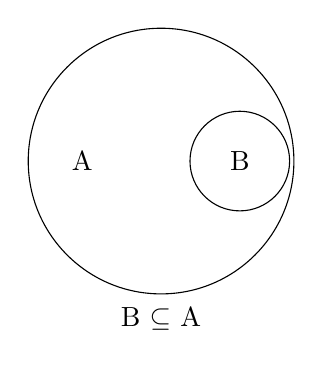
\begin{tikzpicture}
       \node at (0,0) [inner sep=1pt] (A) {A};
       \node at (2,0) (B) {B};
       \draw
          (1,0) circle [draw,radius=48pt] 
          (2,0) circle [draw,clip,radius=18pt];
       \node at (1,-2) {B $\subseteq$ A};
      \end{tikzpicture}}
      {\caption{Inclusion}}
    \ffigbox{%
      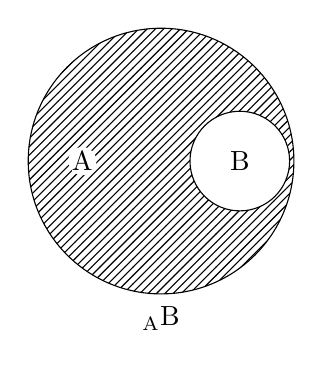
\begin{tikzpicture}
       \node at (2,0) (B) {B};
       \filldraw [even odd rule, pattern=north east lines]
          (1,0) circle [draw,radius=48pt] 
          (2,0) circle [draw,clip,radius=18pt];
       \node at (0,0) [inner sep=0pt, circle, fill=white] (A) {A};
       \node at (1,-2) {$\complement$\textsubscript{A}B}; 
      \end{tikzpicture}}
      {\caption{Complémentaire}}
    \end{floatrow}
    \end{figure}
    
    L’inclusion est une \textstyleTermesapprof{relation d’ordre} (voir la \sectref{sec:3.3.30} \textit{Dépendance, dominance et transitivité} pour une définition formelle) sur les ensembles, similaire à la relation d’ordre ${\leq}$ sur les nombres (d’où la notation \textrm{${\subseteq}$}). Dire «~B \textrm{${\subseteq}$} A~» revient à dire que B est plus petit que A pour la relation d’inclusion. Néanmoins contrairement à la relation ${\leq}$, l’inclusion est un ordre \textstyleTermesapprof{partiel}, puisque deux ensembles peuvent ne pas être ordonnés l’un par rapport à l’autre, notamment lorsqu’ils sont disjoints (c’est-à-dire n’ont pas d’éléments en commun).
                      
    À tout ensemble B inclus dans A, on peut associer le \textstyleTermesapprof{complémentaire} \textrm{${\complement}$}\textsubscript{A}B de B dans A.

    À tout ensemble E, on peut associer l’\textstyleTermesapprof{ensemble des parties} de E, noté 2\textsuperscript{E} ou $\mathcal{P}(\text{E})$, avec un $\mathcal{P}$ comme \textit{partie}. La notation 2\textsuperscript{E} repose sur le fait que si E a \textit{n} éléments, alors 2\textsuperscript{E} a 2\textit{\textsuperscript{n}} éléments.

    Les ensembles \textrm{${\varnothing}$} et E sont respectivement le \textstyleTermesapprof{plus petit} et le \textstyleTermesapprof{plus grand élément} de 2\textsuperscript{E} pour l’inclusion.

    On ne confondra pas l’élément \textit{x} de E avec le \textstyleTermesapprof{singleton} \{~\textit{x}~\}, qui est un élément de 2\textsuperscript{E}.

    On peut définir sur 2\textsuperscript{E} deux opérations binaires, l’union et l’intersection. L’\textstyleTermesapprof{union} de A et B, notée A~\textrm{${\cup}$}~B, est l’ensemble qui contient à la fois les éléments de A et ceux de B, tandis que l’\textstyleTermesapprof{intersection} de A et B, notée A~\textrm{${\cap}$}~B, est l’ensemble des éléments communs à A et B. On peut visualiser ces ensembles sur les schémas suivants :

    \begin{figure}
    \begin{floatrow}
      \captionsetup{margin=.05\linewidth}
      \ffigbox{%
      
\begin{tikzpicture}
       \filldraw[pattern=north east lines]
          (0,0) circle [draw,radius=18pt] 
          (1,0) circle [draw,radius=18pt];
       \node at (0,0) [fill=white, circle, inner sep=0pt] (A) {A};
       \node at (1,0) [fill=white, circle, inner sep=0pt] (B) {B};
       \node at (0.5,-1) {A $\cup$ B};
      \end{tikzpicture}}
    {\caption{Union}}                                                                   
    \ffigbox{%
      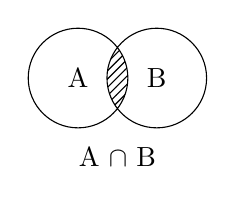
\begin{tikzpicture}
       \node at (0,0) [inner sep=1pt] (A) {A};
       \node at (1,0) (B) {B};
     \begin{scope}
        \clip (0,0) circle [draw,radius=18pt];
        \fill[pattern=north east lines] (1,0) circle [draw,radius=18pt];
      \end{scope}
       \draw
          (0,0) circle [draw,radius=18pt] 
          (1,0) circle [draw,radius=18pt];
       \node at (0.5,-1) {A $\cap$ B};
      \end{tikzpicture}}
    {\caption{Intersection}}
    \end{floatrow}                                                                 
    \end{figure}

    L’ensemble 2\textsuperscript{E} muni des opérations binaires \textrm{${\cap}$} et \textrm{${\cup}$} et de la relation d’ordre \textrm{${\subseteq}$} possède d’excellentes propriétés similaires à celles de l’ensemble des nombres naturels muni des opérations + et \textrm{${\times}$} et de la relation ${\leq}$. En un sens, ces opérations et relations «~structurent~» l’ensemble 2\textsuperscript{E} ; une telle structure est appelée une \textstyleTermesapprof{structure algébrique}.
    }
\maths{Dualité}{%\label{sec:2.2.8}
    L’analyse distributionnelle consiste à classer les éléments en fonction de leur distribution dans des combinaisons avec d’autres éléments. La principale difficulté de l’analyse distributionnelle est que tout est interdépendant et que les éléments servent à se classifier les uns les autres. Il existe ainsi une véritable symétrie entre classes distributionnelles et familles d’environnement. Ce type de symétrie est appelé en mathématique la \textstyleTermesapprof{dualité}. Le \textstyleTermesapprof{dual} d’une classe distributionnelle est la famille des environnements compatibles avec les éléments de la classe et le \textstyleTermesapprof{dual} d’une famille d’environnements est la classe distributionnelle des éléments compatibles avec les environnements de la famille. Autrement dit, si A est une classe distributionnelle, \textbf{dual(A)} \textbf{=} \textbf{famille(A)} = “l’ensemble des environnement compatibles avec A” et, si A est une famille d’environnements, \textbf{dual(A)} \textbf{=} \textbf{classe(A)} = “l’ensemble des signes compatibles avec A”.

    Le schéma suivant illustre la dualité. La dualité lie des \textstyleTermesapprof{objets} à des \textstyleTermesapprof{propriétés~}: dans notre cas, les objets sont les signes et les propriétés les environnements (plus exactement la propriété est la compatibilité avec un environnement). Les propriétés définissent des classes d’objets, tandis que les objets définissent des familles de propriétés. Mais le procédé est totalement symétrique et on peut très bien considérer les propriétés comme nos objets et les objets comme leurs propriétés : dans ce cas, les «~propriétés~» d’une propriété donnée sont les objets compatibles avec elle.

    \begin{figure}
    \caption{Dualité entre objets\slash signes et propriétés\slash environnements}
    %% Kudos to Schrödinger's cat for showing the basic workings
    %% of the 3d TikZ library in an unrelated Question at 
    %% https://tex.stackexchange.com/a/548688
    \begin{tikzpicture}[3d view={45}{45},every node/.style={font=\strut}]
      \begin{scope}[canvas is xy plane at z=0,transform shape]
        \draw (0,0) circle [radius=2.5cm] coordinate (circle1);
        \node (classe) [draw,circle] at (-1,0) {classe(A)};
        \node (B) [draw,circle] at (1.5,0) {B};
        \node[left=2.5cm of circle1] {objets};
        \node[right=2.5cm of circle1] {signes};
      \end{scope}
      \begin{scope}[canvas is xy plane at z=-5,transform shape]
        \draw (0,0) circle [radius=2cm] coordinate (circle2);
        \node (A) [draw,circle] at (-1,0) {A};
        \node (famille) [draw,circle] at (.5,0) {famille(B)};
        \node[left=2cm of circle2] {propriétés};
        \node[right=2cm of circle2] {environnements};
      \end{scope}
    \draw  (A.north) -- (classe.335);
    \draw (B) -- (famille.north);
    \end{tikzpicture}
    \end{figure}

    Si A est une classe distributionnelle ou une famille d’environnements, dual(\linebreak dual(A)) = A. La fonction «~dual~» associe donc une classe à chaque famille, laquelle est elle-même associée à cette classe. On en déduit qu’il y a exactement autant de classes distributionnelles que de familles d’environnements.

    De plus, la fonction «~dual~» possède une excellente propriété qui est de \textbf{préserver la structure algébrique} définie par les opérations \textrm{${\cap}$} et \textrm{${\cup}$} et la relation d’ordre \textrm{${\subseteq}$}, puisque dans les deux cas (que A et B soient des classes ou des environnements), on a :

    \begin{enumerate}
    \item  si A~\textrm{${\subseteq}$}~B, alors dual(B)~\textrm{${\subseteq}$}~dual(A) ; autrement dit, plus on considère d’environnements, moins il y a de signes compatibles.
    \item  dual(A~\textrm{${\cup}$}~B) = dual(A)~\textrm{${\cap}$}~dual(B) ; autrement dit, les signes compatibles avec à la fois les environnements dans A et ceux dans B sont, sans surprise, les signes qui sont à la fois compatibles avec A et compatibles avec B.
    \item dual(A~\textrm{${\cap}$}~B) = dual(A)~\textrm{${\cup}$}~dual(B).
    \end{enumerate}

    La dualité inverse les rôles de \textrm{${\cap}$} et \textrm{${\cup}$}, ce qui ne change rien à la structure, car ces deux opérations sont elles-mêmes duales l’une de l’autre. L’ensemble des classes distributionnelles et l’ensemble des familles ont donc exactement la même structure algébrique et sont le \textbf{miroir l’un} \textbf{de l’autre}.
}
\section{Signème}\label{sec:2.2.9}

Nous nous sommes intéressés jusque-là au découpage des signes linguistiques selon l’\textstyleTermes{axe syntagmatique}, c’est-à-dire selon la façon dont ils se combinent ou peuvent être décomposés. Nous allons maintenant nous intéresser à la délimitation des signes selon l’\textstyleTermes{axe paradigmatique} (voir la \sectref{sec:2.1.7} sur \textit{L’identification des unités de la langue} et l’\encadref{fig:2.2.3} sur \textit{La quatrième proportionnelle}). Nous regardons ici le paradigme des environnements pour les différentes occurrences d’une même forme afin de déterminer s’il s’agit des signifiants d’un même signe ou pas.

Considérons par exemple le segment /\textstylePhono{avãs-}/ de \textit{Le chat avançait}. On va retrouver le même segment /\textstylePhono{avãs-}/ dans des énoncés tel que \textit{Nous} \textbf{\textit{avanç}}\textit{ons grâce au vent} et \textit{L’âne ne veut plus} \textbf{\textit{avanc}}\textit{er}. On peut considérer qu’il s’agit du même signe, car sa forme est identique (l’alternance orthographique \textit{c} vs \textit{ç} n’est pas pertinente, la forme orale est identique) et que sa contribution sémantique est identique : ‘avancer’ signifie ici ‘se déplacer vers l’avant’.

Considérons maintenant d’autres occurrences de /\textstylePhono{avãs-}/ dans d’autres environnements :

\begin{figure}
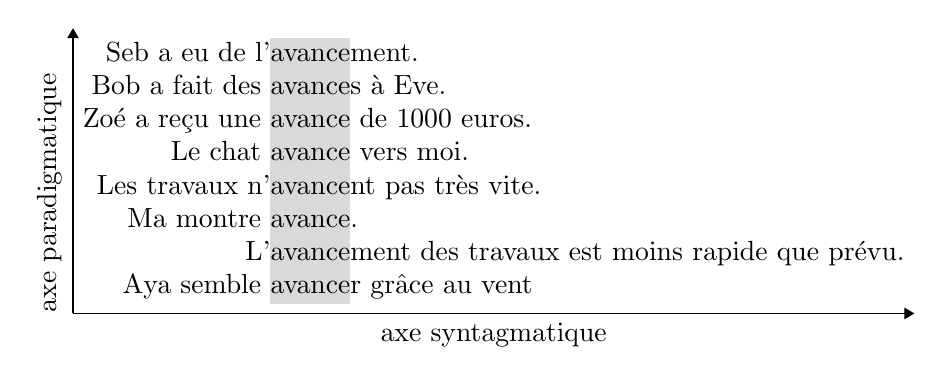
\begin{tikzpicture}
   \matrix (avance) [matrix of nodes,
                     column sep=0pt,
                     every node/.style={inner sep=0pt,font=\strut},
                     column 1/.style={anchor=base east},
                     column 2/.style={nodes={fill=black!15}},
                     column 3/.style={anchor=base west}]
     {
       Seb a eu de l’&avance&ment.\\
       Bob a fait des~~&avance&s à Eve.\\
       Zoé a reçu une~~&avance&~de 1000 euros.\\
       Le chat~~&avance&~vers moi.\\
       Les travaux n’&avance&nt pas très vite.\\
       Ma montre~~&avance&.\\
       L’&avance&ment des travaux est moins rapide que prévu.\\
       Aya semble~~&avance&r grâce au vent\\
     };
   \draw [-{Triangle[]}] (avance.south west) -- (avance.south east) node [midway,below] {axe syntagmatique};
   \draw [-{Triangle[]}] (avance.south west) -- (avance.north west) node [very near end,left=2ex,rotate=90] {axe paradigmatique};
\end{tikzpicture}
\caption{Découpage de /\textstylePhono{avãs-}/ selon les axes paradigmatique et syntagmatique}
\end{figure}

Dans les énoncés \textit{Ma montre} \textbf{\textit{avanc}}\textit{e} ou \textit{Les travaux n’}\textbf{\textit{avanc}}\textit{ent pas très vite}, nous n’avons plus affaire au même signe /\textstylePhono{avãs-}/, car le sens n’est plus ‘se déplacer vers l’avant’. On peut néanmoins considérer qu’il s’agit, d’un certain point de vue, du même segment, car même si le sens est différent, il reste lié au premier sens que nous avons considéré. Il s’agit d’acceptions métaphoriques : lorsque ma montre avance, c’est comme si l’aiguille avançait plus vite que le temps ; lorsque les travaux avancent, ils se rapprochent de leur achèvement. De plus, la forme du signe est exactement la même et sa combinatoire assez similaire : \textit{avanç-} se combine toujours avec -\textit{ait} (\textit{Ma montre} \textbf{\textit{avanç}}\textit{ait}), mais par contre elle n’accepte plus de complément locatif (\textit{L’âne} \textbf{\textit{avanç}}\textit{ait vers moi ; \textsuperscript{\#}}\textit{Ma montre avance vers moi}). Bien qu’il s’agisse de trois signes différents (puisque les signifiés sont différents), nous considérons pourtant qu’ils appartiennent à une même unité, qu’on nomme généralement le verbe \textsc{avancer}.

On retrouve encore le même segment /\textstylePhono{avãs}/ dans~des énoncés tels que \textit{Pierre est en} \textbf{\textit{avance}}, \textit{Pierre a reçu une} \textbf{\textit{avance}} \textit{de 1000 euros, Pierre a fait des} \textbf{\textit{avance}}\textit{s à Marie}. Ici le sens de /\textstylePhono{avãs}/ est différent, mais surtout sa combinatoire est très différente : ce n’est plus un verbe et il ne peut plus se combiner avec un segment tel que -\textit{ait}. La forme est néanmoins identique et la parenté de sens non négligeable. Dans \textit{L’}\textbf{\textit{avance}}\textit{ment des travaux est moins rapide que prévu} ou \textit{Pierre a eu de l’}\textbf{\textit{avance}}\textit{ment}, /\textstylePhono{avãs}/ est encore un signe (\textit{avancement} est à \textit{avancer} ce que \textit{changement} est à \textit{changer}), mais sa combinatoire est encore différente puisqu’il est indissociable de \textit{{}-ment}.

Tout locuteur du français voit un lien entre toutes les occurrences d’/\textstylePhono{avãs}/ que nous avons considérées. Nous considérons donc que, d’un certain point de vue (et d’un certain point de vue seulement), il s’agit toujours du même objet : un tel objet est appelé un signème.

\Definition{\textstyleTermes{signème}}
{Un \textstyleTermes{signème} est un \textbf{ensemble de signes ou de quasi-signes} de \textbf{même forme} et de \textbf{sens apparentés}. (Nous considérerons des signèmes de signes de formes différentes à la \sectref{sec:2.2.20} sur l’\textit{Allomorphie}.)}

On peut repérer à l’intérieur d’un signème des sous-ensembles de signes qui ont une distribution comparable. À l’intérieur du signème /\textstylePhono{avãs}/, on repère ainsi trois (sous-)signèmes : le verbe \textsc{avancer}, le nom \textsc{avance} et le radical \textit{avance-} de \textsc{avancement}.

\loupe{Racine et signème}{%\label{sec:2.2.10}
    Jusqu’où pousser la recherche des segments communs ? Il y a dans les mots \textit{commerce} et \textit{marchand} des segments comparables (/m\textrm{ɛ}rs/ pour \textit{commerce} et /m\textrm{a}r\textrm{ʃ}/ pour \textit{marchand}) qui découlent de fait de la même \textstyleTermesapprofondissement{racine} indo-européenne /m\textrm{ɛ}rk/, que l’on retrouve non altérée dans \textit{mercantile}. Néanmoins, il est probable que les locuteurs ordinaires du français (c’est-à-dire qui ne sont pas entraînés à analyser leur langue) n’auront pas remarqué cela, malgré la forte parenté sémantique de ces mots.

    Qu’est-ce qui distingue racines et morphèmes ?

    Si nous reconnaissons dans \textit{avancement} le même signème /avãs/ que dans \textit{avançons}, c’est parce que \textit{avancement} est à \textit{avançons} ce que \textit{changement} est à \textit{changeons}. Rien de tel pour \textit{commerce} et \textit{marchand} où il n’y a aucune paire analogue. La mise en évidence d’un segment commun ne relève pas de la grammaire du locuteur et de sa connaissance \textbf{de} la langue, mais d’une connaissance \textbf{sur} la langue. Le \textbf{signème} appartient à l’étude \textstyleTermesapprofondissement{synchronique} de la langue, la \textbf{racine} à l’étude \textstyleTermesapprofondissement{diachronique} de la langue et à l’étymologie (l’étude de l’origine des mots). L’opposition entre \textstyleTermesapprofondissement{synchronie} et \textstyleTermesapprofondissement{diachronie} a été posée par Ferdinand de Saussure ; la synchronie considère un état de langue à un moment donné, tandis que la diachronie étudie les variations (du grec \textit{dia-} ‘à travers’) entre différents état de langue selon l’axe temporel (\textit{chronos}).

    Donnons deux autres exemples : \textit{avance, avant} et \textit{avantage} ont aussi une racine commune, comme le suggère les proximités de forme et de sens, mais on ne peut parler d’un même signème, puisqu’aucun des liens qui unissent ces mots n’a d’analogue en français. \textit{État} et \textit{constater} ont également une racine commune : la parenté de sens apparaît quand on pense à la synonymie entre \textit{constater} et \textit{faire état} et la parenté de forme devient évidente quand on pense qu’un autre sens de \textit{état} se dit en anglais \textit{state} (et que l’on a noté qu’il existe d’autres paires en français où un /s/ s’est effacé : \textit{été-estival, hôpital-hospitalier}).
}
\section{Signèmes minimaux : morphème et syntaxème}\label{sec:2.2.11}

Si nous considérons maintenant le signème /\textstylePhono{avãs}/, nous voyons qu’il n’est possible de décomposer aucun de ses éléments en deux signes linguistiques. On peut éventuellement essayer avec un segment /\textstylePhono{avã}/ que l’on trouve dans \textit{La plage est} \textbf{\textit{avant}} \textit{le village}, mais on ne voit pas comment la composition du sens de cet /\textstylePhono{avã}/ avec un éventuel signe /\textstylePhono{s}/ pourrait donner le signe \textit{avanç-} /\textstylePhono{avãs-}/. Proposer un signe \textstylePhono{/s/} n’aurait de sens qu’au cas où pour un autre signe X au moins, l’ajout d’un \textstylePhono{/s/} créait le sens ‘se déplacer dans la direction X’, c’est à dire si /\textstylePhono{avã}/ et /s/ se combinaient proprement. Le signème /\textstylePhono{avãs}/ est donc indécomposable.

\Definition{\textstyleTermes{morphème}}
{Un \textstyleTermes{morphème} est un signème dont aucun signe n’est décomposable proprement.}

Les morphèmes sont donc les signèmes minimaux du point de vue de l’opération de combinaison propre ${\boxplus}$. Nous pouvons considérer de même les signèmes minimaux du point de vue de la combinaison libre ${\oplus}$, que nous appelons les syntaxèmes.

\Definition{\textstyleTermes{syntaxème}}
{Un \textstyleTermes{syntaxème} est un signème de signes de la même classe distributionnelle dont certains se combinent librement et dont aucun n’est une combinaison libre de signes.}

Les morphèmes sont les \textbf{unités minimales de la morphologie} et les syntaxèmes sont les \textbf{unités minimales de la syntaxe}. La définition des syntaxèmes sera précisée dans le \chapref{sec:3.1}.

Reprenons l’exemple du signème /\textstylePhono{avãs}/ : il s’agit d’un morphème, puisqu’aucun de ses éléments n’est décomposable proprement. Il contient deux syntaxèmes que sont \textsc{avancer} et \textsc{avance}. Enfin, \textsc{avancement} est un syntaxème, puisqu’aucune de ses acceptions n’est décomposable librement (seul un petit nombre de morphèmes verbaux permettent la combinaison avec \textit{{}-ment}). Il est néanmoins décomposable proprement et contient une occurrence du morphème /\textstylePhono{avãs}/.

\loupe{Les termes \textit{morphème} et autres \textit{X-èmes}}{%\label{sec:2.2.12}
    La première étude des règles morphologiques d’une langue remonte à 2500 ans au moins. Il s’agit de l’extraordinaire description du sanskrit védique faite par le linguiste indien Pā\textrm{ṇ}ini, qui comprend une description des morphèmes du sanskrit et des règles de combinaison de leurs signifiants. Les termes \textit{morphème} et \textit{phonème} sont introduits dans les années 1880 par le linguiste polonais Baudouin de Courtenay. La définition formelle des morphèmes et le principe de commutation doivent beaucoup aux travaux des distributionnalistes américains sur les langues amérindiennes (voir l’\encadref{fig:2.1.8} sur \textit{Structuralisme et distributionnalisme}).

    Les termes en -\textit{ème} vont foisonner au cours du 20\textsuperscript{e} siècle. Les termes \textit{lexème} et \textit{grammème} sont couramment utilisés pour désigner respectivement les unités du lexique et celles de la grammaire. Nous introduisons \textit{syntaxème} pour désigner les unités minimales de la syntaxe, qu’elles soient lexicales comme le \textit{lexème} ou grammaticales comme le \textit{grammème}. Le terme \textit{syntaxème} (ou la variante \textit{syntactème}) a été utilisé marginalement par quelques auteurs, mais ne s’est jamais imposé, d’autant que c’est le mot qui est généralement considéré comme l’unité minimale de la syntaxe (contrairement au point de vue défendu ici qui considère qu’il s’agit du syntaxème). Le terme \textit{sémantème}, que nous utiliserons pour désigner les unités minimales de la sémantique, est beaucoup plus courant et a été utilisé par Charles Bally ou Igor Mel’čuk pour désigner les sens lexicaux. Nous lui donnons un sens un peu différent en l’utilisant pour désigner des signes (et pas seulement des signifiés) (voir \chapref{sec:2.3} sur \textit{Sémantèmes et syntaxèmes}). Tous les termes que nous venons de mentionner (\textit{morphème, lexème, grammème, syntaxème, sémantème}) désignent, dans l’acception dans laquelle nous les utilisons, des ensembles de signes. Pour finir, nous introduisons le terme \textit{signème} pour désigner tout ensemble de signes d’un de ces types.
}
\section{Lexème, flexion et grammème}\label{sec:2.2.13}

On distingue deux principaux types de syntaxèmes : les syntaxèmes lexicaux ou lexèmes et les syntaxèmes flexionnels ou grammèmes.

\begin{itemize}
\item \textsc{avancer} est un \textstyleTermes{syntaxème lexical} ou \textstyleTermes{lexème~}: il appartient à une classe distributionnelle \textstyleTermes{ouverte} de syntaxèmes, c’est-à-dire qu’il peut commuter avec un très grand nombre de syntaxèmes, potentiellement illimité (cet ensemble est celui des verbes). De plus, ses sens sont assez précis pour être paraphrasés. Par exemple, dans l’énoncé \textit{Le chat avançait}, \textsc{avancer} signifie ‘se déplacer vers l’avant’ et il commute avec sa définition : \textit{Le chat se déplaçait vers l’avant} est une paraphrase de \textit{Le chat avançait}.
\item {}-\textit{ait} est une \textstyleTermes{flexion}. Il s’agit d’une combinaison de plusieurs syntaxèmes, qui comprend notamment la combinaison libre d’un temps (l’imparfait) et d’un accord en nombre et personne. Les syntaxèmes qui composent une flexion s’appellent des \textstyleTermes{syntaxèmes flexionnels} ou \textstyleTermes{grammèmes}. Flexions et syntaxèmes flexionnels appartiennent à des classes distributionnelles \textstyleTermes{fermées} d’éléments, c’est-à-dire qu’ils commutent avec un nombre restreint d’éléments similaires dont on peut faire la liste exhaustive (il y a par exemple 51 flexions possibles pour un verbe du français : 6 formes pour chacun des 7 «~temps~» simples, 4 formes pour chacun des deux participes, auxquelles il faut encore ajouter la forme infinitive ; 51 = 7${\times}$6 + 2${\times}$4 + 1). Les grammèmes expriment des significations grammaticales qui ne peuvent être paraphrasées facilement.
\end{itemize}

Lexème verbal et flexion ne peuvent donc pas être utilisés de manière \textstyleTermes{autonome}. Le lexème et sa flexion sont \textstyleTermes{indissociables} l’un de l’autre : une flexion verbale ne s’utilise pas sans une base verbale et un lexème verbal ne s’utilise pas sans flexion. Ceci nous amène à la définition du mot, sur laquelle nous reviendrons au \chapref{sec:4.1} : un \textstyleTermes{mot} est grosso modo un signe linguistique autonomisable minimal, c’est-dire dont les parties sont indissociables et donc non-autonomisables.

Du fait que les lexèmes verbaux ne sont pas autonomisables, il est d’usage de les nommer par l’une de leurs formes fléchies. L’usage en français est d’utiliser la forme infinitive. Cet usage est purement conventionnel (et pédagogiquement assez mauvais puisque le radical de l’infinitif n’est généralement pas le radical de base ; voir l’\encadref{fig:2.2.23} sur \textit{Syntaxème zéro et troncation en français}) ; par exemple en grammaire latine, il est d’usage de nommer un lexème verbal par la forme de la 1\textsuperscript{ère} personne du singulier du présent (lat. \textsc{amo} ‘j’aime’) et en grammaire arabe par la forme de la 3\textsuperscript{ème} personne du singulier du passé (ar. \textsc{kataba} ‘il a écrit’). Pour éviter toute confusion entre le lexème et la forme infinitive, nous notons le premier en petites majuscules, \textsc{avancer}, et la deuxième en italique, \textit{avancer}. Les syntaxèmes flexionnels sont désignés par des termes métalinguistiques : présent, pluriel, etc. La forme \textit{avancer} est la combinaison de \textsc{avancer} et de l’infinitif :

\ea
\textit{avancer} = \textsc{avancer} ${\oplus}$ infinitif.
\z

\section{Signème libérable, radical, affixe}\label{sec:2.2.14}

Nous allons caractériser les occurrences des morphèmes au sein des lexèmes, c’est-à-dire les \textstyleTermes{morphèmes sous-lexicaux}. Un lexème qui peut être décomposé en plusieurs morphèmes est dit \textstyleTermes{complexe}.

\Definition{\textstyleTermes{libérable}, \textstyleTermes{morphème libérable}, \textstyleTermes{lexical}}
{Un signème est dit \textstyleTermes{libérable} s’il existe des environnements dans lesquels ce signème commute librement. Un \textstyleTermes{morphème libérable} est donc un morphème qui contient un syntaxème. Lorsque ce syntaxème est lexical, le morphème est dit \textstyleTermes{lexical}.}

Cette propriété est utilisée pour classifier les morphèmes constitutifs d’un lexème complexe. Si l’on considère le syntaxème \textit{brûlure}, qui se décompose en \textit{brûl}${\boxplus}$\textit{ure}, on constate que \textit{brûl-} est libérable, puisqu’il commute librement dans \textit{nous brûlons}, mais \textit{{}-ure} n’est pas libérable, puisqu’il n’existe aucun environnement où -\textit{ure} commute librement.

\Definition{\textstyleTermes{radical}, \textstyleTermes{affixe}, \textstyleTermes{préfixe}, \textstyleTermes{suffixe}}
{Un morphème, lorsqu’il est l’unique morphème lexical d’un lexème, est appelé le \textstyleTermes{radical} du lexème. Un morphème non lexical est appelé un \textstyleTermes{affixe}. Lorsqu’il précède le radical, il s’agit d’un \textstyleTermes{préfixe} et lorsqu’il le suit d’un \textstyleTermes{suffixe}.}

Il existe également des lexèmes construits uniquement avec des morphèmes non libérables. En français, un certain nombre de lexèmes, appelés composés savants, sont construits avec deux morphèmes lexicaux empruntés au grec ancien (dont certains sont devenus libérables) : \textit{sismo}${\boxplus}$\textit{graphe, sismo}${\boxplus}$\textit{logue, grapho}${\boxplus}$\textit{logue, géo}${\boxplus}$\textit{graphe, géo}${\boxplus}$\textit{thermie, thermo}${\boxplus}$\textit{mètre, métro}${\boxplus}$\textit{nome}, etc. De tels morphèmes, dont le statut est intermédiaire entre affixe et radical, sont appelés des \textstyleTermes{confixes}, car ils doivent être associés par paire pour former un lexème.

Il faut noter que les termes de \textit{libre} et de \textit{libérable} sont définis par des critères purement distributionnels et recouvrent donc des notions syntaxiques. Ils ne doivent pas être confondus avec un autre emploi du terme \textit{libre} dû à Bloomfield qui est proche de ce que nous avons appelé l’autonomisabilité et qui conduit à appeler \textit{forme liée} tout affixe. Dans notre terminologie, au contraire, les \textbf{syntaxèmes flexionnels}, bien qu’étant des affixes, se combinent librement par définition et sont parfaitement \textbf{libérables}. Par contre, ils ne sont \textbf{pas autonomisables}, puisqu’ils sont indissociables de lexèmes.

Les notions de radical et d’affixe doivent être étendues par analogie. Ainsi, un quasi-morphème comme \textit{struct-}, bien que non libérable, est également considéré comme un élément lexical et comme le radical de \textit{structure} et de \textit{construction}, car il commute avec des morphèmes lexicaux.

A l’inverse, certains préfixes du français présentent un cas limite d’affixe, puisqu’ils appartiennent à des morphèmes prépositionnels comme le \textit{en} de \textit{il} \textbf{\textit{en}}\textit{terre} ou le \textit{sur} de \textit{il} \textbf{\textit{sur}}\textit{estime}. On considère quand même qu’il s’agit d’affixes, car les prépositions simples forment une classe fermée et sont donc moins lexicales que les morphèmes qui ont des emplois en tant que syntaxèmes appartenant à des classes ouvertes. De plus, la classe distributionnelle des préfixes du français contient quand même une bonne proportion de morphèmes non libérables, comme \textit{con-} ou \textit{in-}, et qui commutent avec les autres (\textbf{\textit{com}}\textit{prendre} vs \textbf{\textit{sur}}\textit{prendre}, \textbf{\textit{in}}\textit{estimable} vs \textbf{\textit{sur}}\textit{estimer}).

\section{Dérivation et composition}\label{sec:2.2.15}

La plupart des lexèmes complexes du français sont construits avec un radical et un certain nombre d’affixes. Par exemple, le lexème \textit{détournement} est construit avec le radical \textit{tourn-}, le préfixe \textit{dé-} et le suffixe \textit{{}-ment}. Les lexèmes complexes comportant un unique morphème lexical sont appelés des \textstyleTermes{dérivés morphologiques}. L’opération qui consiste à ajouter un affixe à un lexème pour former un nouveau lexème est appelée la \textstyleTermes{dérivation morphologique}.

Il existe aussi des lexèmes construits avec plusieurs morphèmes lexicaux, comme \textit{soutien-gorge} ou \textit{bonhomme} : de tels syntaxèmes sont appelés des \textstyleTermes{composés morphologiques}. L’opération qui consiste à combiner deux lexèmes pour former un nouveau syntaxème est appelée la \textstyleTermes{composition morphologique}. Un composé peut être la source d’une dérivation comme dans \textit{bonhommie}.

On peut associer à un lexème complexe une structure morphologique en regardant les portions du lexème qui sont libérables. Une \textstyleTermes{unité morphologique} est soit un morphème, soit une portion libérable d’un lexème. Les unités morphologiques de \textit{détournement} sont les morphèmes \textit{dé-, tourn-} et -\textit{ment} et les combinaisons \textit{détourn-} (\textit{il} \textbf{\textit{détourn}}\textit{ait}) et \textit{détournement.} Par contre °\textit{tournement} n’est pas libérable. On en déduit une \textstyleTermes{structure morphologique} que nous pouvons représenter dans ce cas par un parenthésage : \textit{détournement} = (\textit{dé}${\boxplus}$\textit{tourn})${\boxplus}$\textit{ment}. Ceci induit un \textstyleTermes{chemin dérivationnel} menant du radical du lexème au lexème complet par combinaisons successives de morphèmes. Pour \textit{détournement}, le chemin est \textit{tourn}(\textit{er}) → \textit{détourn}(\textit{er}) → \textit{détournement} et pas \textit{tourn}(\textit{er}) → °\textit{tournement} → \textit{détournement}. Cela signifie que, dans la façon dont est perçu le lexème \textit{détournement}, c’est \textit{dé}{}- qui s’affixe d’abord à \textit{tourn}{}-, puis -\textit{ment} au tout.

L’étude des \textstyleTermes{morphèmes sous-lexicaux}, c’est-à-dire des occurrences d’un morphème à l’intérieur d’un lexème, ne relève pas de la syntaxe et est donc hors de la visée de cet ouvrage. Une telle étude concerne la construction des lexèmes, c’est-à-dire la \textstyleTermes{morphologie constructionnelle} et la \textstyleTermes{lexicologie}. Cette notion est néanmoins essentielle à la compréhension de ce que sont les syntaxèmes et de ce qui les différencie des occurrences liées des morphèmes.

\loupe{«~Syntaxe~» des morphèmes sous-lexicaux}{%\label{sec:2.2.17}
    Lorsqu’on parle de syntaxe, on parle normalement de combinatoire libre (voir la \sectref{sec:3.1.6} sur \textit{Syntaxe et morphologie}) et lorsqu’on parle de combinatoire libre, on parle de combinaisons qui sont faites par le locuteur au moment de la production d’un nouvel énoncé (voir l’\encadref{fig:2.2.6} sur \textit{Liberté de combinaison et opposition parole/langue}). La combinatoire des sous-morphèmes relève au contraire de la structure d’unités déjà construites et stockées dans le lexique mental du locuteur (même s’il existe la possibilité de construire de nouvelles unités lors de la production avec les constructions productives). Il en découle que l’histoire constructionnelle de ces unités se fait sur un temps beaucoup plus long, bien qu’il en reste des traces en synchronie (par la commutation propre avec d’autres morphèmes). On peut alors se poser la question suivante : la structure des combinaisons de sous-morphèmes est-elle ou non de la même nature que celle des syntaxèmes ?

    Nous étudierons en détail la structure des combinaisons syntaxiques dans la partie 3, dont c’est le sujet central. Les outils que nous introduirons peuvent aussi s’appliquer à la description des combinaisons morphologiques. Nous opposerons en particulier deux approches principales de la structure syntaxique, la structure de dépendance et la structure de constituants. La principale différence entre les deux approches reposent sur ce qu’elles encodent prioritairement (voir l’\encadref{fig:3.4.16} \textit{Dépendance et constituance se complètent}). Les structures de constituants permettent d’encoder naturellement l’ordre dans lequel les combinaisons ont lieu et c’est ce que nous avons utilisé pour présenter l’analyse de \textit{détournement}, car nous voulions indiquer que lors de l’histoire dérivationnelle de ce mot, \textit{tourn-} s’est d’abord combiné avec \textit{dé-}, puis \textit{{}-ment}. Ils existent des cas où l’histoire dérivationnelle n’est pas aussi claire en synchronie. Tel est le cas par exemple de \textit{châtaigneraie, pommeraie} ou \textit{orangeraie}. Il s’agit a priori du suffixe \textit{{}-aie} qui appliqué à un nom d’arbre désigne un groupe d’arbre, comme dans \textit{chênaie} ‘groupe de chênes’ ou \textit{peupleraie} ‘groupe de peupliers’, avec en plus une alternance -\textit{ier} /je/ → -\textit{er} /ʁ/. On aurait donc \textit{châtaigneraie} = (\textit{châtaigne}\textrm{${\boxplus}$}\textit{ier})\textrm{${\boxplus}$}\textit{aie}. Mais on peut aussi analyser ces dérivations comme le résultat direct de l’application du suffixe \textit{{}-eraie}, lequel suffixe se rencontre dans \textit{chêneraie} ‘groupe de chênes’ (lexème considéré comme fautif mais largement attesté). On peut représenter cette ambiguïté en utilisant une représentation non parenthésée de la dérivation (\textit{châtaigneraie} = \textit{châtaigne}\textrm{${\boxplus}$}\textit{ier}\textrm{${\boxplus}$}\textit{aie}), qui s’apparente alors à une structure de dépendance, puisqu’on n’indique que \textit{{}-ier} se combine aussi bien avec \textit{châtaigne} que \textit{{}-aie} sans spécifier quelle combinaison a lieu en premier.
}
\loupe{Sémantique des morphèmes sous-lexicaux}{%\label{sec:2.2.18}
    Le fait qu’un affixe soit toujours un morphème non libérable influe sur la nature même de son sens : l’affixe ne peut jamais être «~isolé~» et son sens ne peut pas être saisi de manière autonome. Le sens d’un affixe n’apparaît que dans la \textbf{relation entre deux lexèmes} : le sens de -\textit{ure} naît de la relation entre \textsc{blessure} et \textsc{blesser}. Ainsi le sens d’un tel morphème est nécessairement de nature \textbf{opératoire} : il n’est exprimable que dans la relation entre deux sens. Le sens de -\textit{ure} est le sens de l’opération qui permet de construire ‘blessure’ à partir de ‘blesser’ et d’autres paires du même type : une X-ure est le résultat obtenu en X-ant.

    Il existe aussi des morphèmes, comme le -\textit{aume} de \textit{royaume,} qui n’apparaissent que dans un seul lexème dont la diagrammaticité est suffisamment claire pour qu’on attribue un sens au morphème : le fait que le lien sémantique entre \textit{royaume} et \textit{roi} soit assez simple (un royaume est le territoire sous la tutelle d’un roi) et que la paire \textit{roi}{}-\textit{royaume} soit parallèle à d’autres paires comme \textit{prince}{}-\textit{principauté} ou \textit{duc}{}-\textit{duché}, permet de définir facilement le sens (opératoire) de -\textit{aume}. Par contre, \textit{fur}, qui est pourtant un mot, mais qui n’apparaît que dans \textit{au fur et à mesure} n’a plus de sens accessible en français contemporain, car la construction dans laquelle il entre est isolée et qu’il n’y a jamais de commutation possible sur \textit{fur}. De même, beaucoup de locuteurs du français vont utiliser une locution comme \textit{être dans le collimateur} sans avoir aucune idée de ce qu’est un collimateur (voir la \sectref{sec:3.1.3} sur \textit{Le collimateur et la sellette} pour d’autres exemples).
}
\eiffel{À la limite entre morphème sous-lexical et syntaxème flexionnel}{%\label{sec:2.2.19}
    La notion de commutation libre est \textstyleTermesapprofondissement{graduelle} et il est parfois difficile pour certains morphèmes de les situer entre morphème sous-lexical et syntaxème (flexionnel). Le cas du morphème -\textit{ment} qui transforme un adjectif en adverbe est un cas intéressant de morphème qui ne commute pas librement, mais s’en approche néanmoins. Dans de nombreux cas, le changement de partie du discours opéré par \textit{{}-ment} ne s’accompagne d’aucun changement de sens, ce qui signifie que la commutation est propre : cf. le passage de \textit{un départ rapide} à \textit{partir rapidement} ou de \textit{une réflexion intense} à \textit{réfléchir intensément}. Mais la dérivation en -\textit{ment} n’est pas systématiquement possible : cf. \textit{une réflexion poussée}/\textit{élaborée} vs *\textit{réfléchir poussément}/\textit{élaborément}, \textit{un départ inattendu} vs *\textit{partir inattendument}. Même des adjectifs très courant comme \textsc{gros} n’ont pas d’adverbe correspondant : \textit{faire une grosse erreur} vs *\textit{se tromper grossement}. Certains adverbes en -\textit{ment} sont fort peu diagrammatiques et ne peuvent pas être décomposés proprement, comme \textit{vraiment}, \textit{carrément} ou \textit{vertement}. En conséquence, la classe des éléments qui se combine avec \textit{{}-ment} comporte pas mal d’irrégularités et est par exemple différente de la classe des adjectifs qui se combinent avec \textit{de façon}, puisqu’on a \textit{de façon poussée, élaborée} ou \textit{inattendue} et pas \textit{de façon verte}. On peut également noter quelques irrégularités morphologiques (voir la \sectref{sec:2.2.20} sur l’\textit{Allomorphie}) dans la combinaison de \textit{{}-ment} et d’un adjectif, toutefois la combinaison libre des verbes avec leur flexion comprend davantage encore d’idiosyncrasies, donc les arguments purement morphologiques ne permettent pas de décider s’il s’agit de combinaison libre ou non.

    Un autre cas discutable est le «~genre~» des noms. Le genre des noms ne doit pas être confondu avec le genre des adjectifs. Le genre des adjectifs est un syntaxème flexionnel qui se combine librement avec l’adjectif. Il n’a aucune contribution sémantique et sert seulement à mieux marquer la dépendance entre le nom et l’adjectif qui le qualifie (ce rôle syntaxique constitue la signification du syntaxème flexionnel). Certains noms varient apparemment en genre comme \textit{lion} vs \textit{lionne}, \textit{acteur} vs \textit{actrice} ou \textit{prince} vs \textit{princesse}. Mais dans ce cas, l’opposition est sémantique et marque une opposition de sexe : la lionne est la femelle du lion. Elle peut s’accompagner d’une variation de sens plus importante, puisque par exemple un prince est toujours le fils d’un roi, tandis qu’une princesse peut être la fille d’un roi ou la femme d’un prince. De même, un lion et une lionne possèdent des différences morphologiques suffisamment importantes, comme la crinière, pour qu’il soit bizarre de dire qu’une lionne est un lion femelle. De plus, cette alternance de genre est assez capricieuse avec de nombreux noms dons le genre est fixe (\textit{grenouille, girafe, chacal, moustique,} etc.), même si l’alternance de sexe reste signifiante et plusieurs cas où deux formes sans liens morphologiques existent (\textit{poule} et \textit{coq} ou \textit{jument} et \textit{étalon}). Citons encore les nombreux trous que des néologismes comme \textit{auteure} ou \textit{professeure} peinent encore à combler. Il y a donc toutes les raisons de considérer le /\textstylePhonoApprofondissement{ɛs}/ de /\textstylePhonoApprofondissement{pr\~{ɛ}sɛs}/ \textit{princesse} comme un morphème sous-lexical plutôt qu’un syntaxème flexionnel.
}
\section{Allomorphie}\label{sec:2.2.20}

Nous n’avons jusque-là considéré que des signèmes dont tous les éléments ont le même signifiant. Il y a néanmoins de bonnes raisons d’élargir la notion de signème et d’accepter des alternances de formes. Ainsi là où le verbe \textsc{avancer} présente une seule forme /\textstylePhono{avãs-}/, le verbe \textsc{aller} présentent quatre formes : /\textstylePhono{v/-} dans \textit{tu} \textbf{\textit{v}}\textit{as}, /\textstylePhono{al/-} dans \textit{nous} \textbf{\textit{all}}\textit{ons}, /\textstylePhono{i/-} dans \textit{nous} \textbf{\textit{i}}\textit{rons}, /\textstylePhono{aj/-} dans \textit{qu’il} \textbf{\textit{aill}}\textit{e}. On veut pourtant regrouper ces formes parce que \textbf{\textit{all}}\textit{+ons} est à \textit{avanç+ons} ce que \textbf{\textit{i}}\textit{+rons} est à \textit{avance+rons}. Nous dirons que \textit{all-} et \textit{i-} sont des allomorphes.

\Definition{\textstyleTermes{allomorphes}}
{Pour que les signes A\textsubscript{1} et A\textsubscript{2} soient des \textstyleTermes{allomorphes}, il faut que A\textsubscript{1} et A\textsubscript{2} aient des signifiants différents, mais qu’il existe un signe A’ et un certain nombre de signes B et B’ tels que A\textsubscript{1}+B soit à A\textsubscript{2}+B’ ce que A’+B est à A’+B’.}

Cette propriété est bien vérifiée par notre premier exemple : A\textsubscript{1} = \textit{al-}, A\textsubscript{2} = \textit{i-}, A’ = \textit{avanç-}, B = \textit{{}-ons}, B’ = -\textit{rons} et A\textsubscript{1}+B = \textit{allons} est à A\textsubscript{2}+B’ = \textit{irons} ce que A’+B = \textit{avançons} est à A’+B’ = \textit{avancerons}. Deux allomorphes sont donc des signes différents, puisqu’ils ont des signifiants différents, mais ils se comportent ensemble comme s’ils formaient un unique signe, puisqu’ils commutent avec un même signe A’. On traduit cela en demandant qu’ils commutent proprement avec un tel signe dans un certain nombre d’environnements.

La notion d’allomorphie nous permet d’étendre la notion de morphème.

\Definition{\textstyleTermes{morphème polymorphique}, \textstyleTermes{morphe}}
{Un \textstyleTermes{morphème polymorphique} est la réunion de plusieurs «~morphèmes~» de formes différentes qui sont des allomorphes les uns des autres. Un \textstyleTermes{morphe} est un sous-ensemble de signes d’un morphème qui possèdent le même signifiant.}

La première propriété que nous avons donnée pour définir l’allomorphie n’est pas suffisante. Une autre propriété nécessaire pour être des allomorphes est de se ressembler. Il y a en fait deux types de ressemblance possibles et ainsi deux notions d’allomorphie : l’une, syntaxique, est une allomorphie au sein d’un syntaxème, basée sur une similarité de syntactique ; l’autre, morphologique, est une allomorphie au sein d’un morphème, basée sur la similarité des formes.

\Definition{\textstyleTermes{allomorphes (syntaxiques)}}
{Les signes A\textsubscript{1} et A\textsubscript{2} sont des \textstyleTermes{allomorphes (syntaxiques)} si A\textsubscript{1} et A\textsubscript{2} ont des formes différentes, mais des sens identiques et s’il existe un syntaxème A’ dont l’ensemble des contextes possibles réunit les contextes possibles de A\textsubscript{1} et A\textsubscript{2}.}

Le cas de \textsc{aller} vu précédemment illustre l’allomorphie syntaxique. La réunion des paradigmes de flexion des différents allomorphes de \textsc{aller} comprend 51 formes et est équivalent au paradigme de flexion de n’importe quel verbe.

Un autre exemple d’allomorphie syntaxique est l’alternance des formes /ɛ/ vs /j/ pour l’imparfait. En effet, ces deux formes ont exactement les mêmes sens et elles possèdent, à elles deux, la même extension que le syntaxème zéro du présent ou le syntaxème /ʁ/ du futur.

Le deuxième cas d’allormorphie nous concerne moins, car il ne relève pas de la syntaxe.

\Definition{\textstyleTermes{allomorphes (morphologiques)}}
{Les signes A\textsubscript{1} et A\textsubscript{2} sont des \textstyleTermes{allomorphes (morphologiques)} si A\textsubscript{1} et A\textsubscript{2} ont des formes différentes mais similaires, des sens apparentés et s’il existe des signes A’, B et B’ tels que A\textsubscript{1}+B soit à A\textsubscript{2}+B’ ce que A’+B est à A’+B’.}

Dans le cas de l’allomorphie morphologique, il n’y a plus identité de sens et la combinatoire est généralement très différente : il faut donc que A\textsubscript{1} et A\textsubscript{2} possèdent une proximité formelle suffisante pour qu’on considère qu’ils sont parents. Par exemple, \textit{écriv}{}- et \textit{écrit}{}- sont des allomorphes, car \textit{écrit+ure} est à \textit{écriv+ons} ce que \textit{sculpt+ure} est à \textit{sculpt+ons} et /ekʁit/ et /ekʁiv/ sont formellement proche. La différence de forme peut être plus importante si elle se retrouve plusieurs fois : \textit{construct}{}- et \textit{construis}{}- sont des allomorphes, car \textit{construction} est à \textit{construisons} ce que \textit{instruction} est à \textit{instruisons} ou ce que \textit{destruction} est à \textit{détruisons}.

Par contre, même si \textit{coup} est à \textit{frapp+ons} ce que \textit{gifle} est à \textit{gifl+ons}, on ne dira pas que \textit{coup} est un allomorphe de \textit{frapp-}. Il y a là une trop grande distance formelle. On dira plutôt que \textit{coup} est un \textstyleTermes{supplétif} de \textit{frapp-}.

En général, les allomorphes d’un signème sont en \textstyleTermes{distribution complémentaire}, c’est-à-dire que leurs environnements respectifs sont incompatibles (voir la notion de \textit{complémentaire} en \textit{Théorie des ensembles} dans la \sectref{sec:2.2.7}). Mais il existe aussi des cas d’alternance de forme dans un même environnement. Par exemple le verbe \textsc{balayer} possèdent deux allomorphes /\textstylePhono{balɛ}/ et /\textstylePhono{balɛj}/ qui peuvent alterner avec certaines flexions : \textit{ils balaient} vs \textit{ils balayent}.

\eiffel{Alternance vocalique en français : allomorphie ou alternance phonologique ? }{%\label{sec:2.2.21}
    Identifier le nombre d’allomorphes d’un morphème ne va pas nécessairement de soi. Ainsi le verbe \textsc{céder} alterne apparemment deux formes : \textit{céd}{}- [\textstylePhonoApprofondissement{sed}] dans \textit{nous cédons} et \textit{cèd}{}- [\textstylePhonoApprofondissement{sɛd}] dans \textit{il cède}. Si [e] et [\textstylePhonoApprofondissement{ɛ}] peuvent être distinctifs dans les syllabes ouvertes (CV) finales (cf. l’opposition entre \textit{été} /\textstylePhono{ete}/ vs \textit{était} /\textstylePhono{etɛ}/ en français parisien), ils se neutralisent dans les autres positions et forment ce qu’on appelle un archiphonème, que nous noterons /\textstylePhonoApprofondissement{E}/ : en syllabe fermée, /\textstylePhonoApprofondissement{E}/ est prononcé [\textstylePhonoApprofondissement{ɛ}] et, en syllabe ouverte non finale, il est prononcé /\textstylePhonoApprofondissement{e}/. Ainsi l’alternance relève complètement de la phonologie du français et \textsc{céder} possède donc un unique morphe /\textstylePhonoApprofondissement{cEd}/. La situation est différente pour \textsc{appeler} qui présente une \textstyleTermes{alternance} entre \textit{appell}{}- /\textstylePhonoApprofondissement{apɛl}/ dans \textit{il appelle} et \textit{appel}{}- /\textstylePhonoApprofondissement{apəl}/ dans \textit{nous appelons~}: ici l’alternance n’a plus de motivation phonologique en français contemporain et il y a bien allomorphie. Le fait que la distribution des deux allomorphes de \textsc{appeler} soit identique à celle des deux prononciations de \textsc{céder} laisse supposer que cette allomorphie résulte d’une alternance phonologique aujourd’hui morte, du même type que celle bien vivante de \textsc{céder}. Une allomorphie de même distribution (et de même origine) se trouve avec les verbes \textsc{mourrir} ou \textsc{pouvoir} (\textit{il} \textbf{\textit{meur}}\textit{t} vs \textit{nous} \textbf{\textit{mour}}\textit{ons}, \textit{il} \textbf{\textit{peu}}\textit{t} vs \textit{nous} \textbf{\textit{pouv}}\textit{ons}). Nous verrons un autre cas distributionnellemnt similaire à l’allomorphie avec les verbes dit du 2\textsuperscript{ème} groupe (dans l’\encadref{fig:2.2.25} sur \textit{Syntaxème zéro et troncation en français}).
}
\section{Amalgame, alternance et mégamorphe}\label{sec:2.2.22}

Nous avons fait jusque-là comme si les signifiants se combinaient de manière \textstyleTermes{concaténative}, c’est-à-dire en s’enchaînant les uns à la suite des autres. Il existe certaines situations où il est difficile de trouver la limite entre un lexème et sa flexion. Par exemple, la forme verbale [\textit{nous}] \textit{sommes} entre dans le paradigme des formes du verbe \textsc{être} et se décompose normalement en un morphe du morphème \textsc{être} et une flexion. Les formes en \textit{{}-mes} de la 1\textsuperscript{ère} personne du pluriel ne se rencontrent plus qu’au passé simple (\textit{nous chant}+\textit{â}+\textit{mes}) et de surcroît aucune autre forme de \textsc{être} n’a le radical \textit{som-}. Il s’agit donc, pour \textit{sommes}, d’une forme amalgamée exprimant conjointement le lexème \textsc{être} et sa flexion.

\Definition{\textstyleTermes{indécomposable}, \textstyleTermes{amalgame}, \textstyleTermes{mégamorphe fort}, \textstyleTermes{cumulative}}
{Une combinaison de syntaxèmes dont le signifiant est \textstyleTermes{indécomposable} est appelée un \textstyleTermes{amalgame} ou \textstyleTermes{mégamorphe fort}. Les syntaxèmes au sein d’un amalgame sont réalisés de manière \textstyleTermes{cumulative}.}

Même des syntaxèmes normalement réalisés par des mots séparés peuvent s’amalgamer, comme \textit{au} /\textstylePhono{o}/ en distribution complémentaire avec \textit{à la} /\textstylePhono{ala}/. Les flexions, c’est-à-dire les combinaisons de syntaxèmes flexionnels, sont souvent des mégamorphes forts : par exemple, si on considère que l’accord verbal -\textit{ons} /\textstylePhono{ɔ}/ combine un accord en personne (1\textsuperscript{ère} personne) et un accord en nombre (pluriel) (voir discussion sur ce point dans la \sectref{sec:4.2.13} sur les \textit{Catégories flexionnelles abstraites}), cette combinaison est un mégamorphe fort.

Un signe tel que \textit{chevaux} \textstylePhono{/ʃəvo/ pose un problème un peu différent. Ici le principe de commutation s’applique à l’ensemble du signe, signifiant compris : \textit{chevaux} est à \textit{cheval} ce que \textit{animaux} est à \textit{animal}. Il n’est néanmoins pas satisfaisant de décomposer \textit{chevaux} en \textit{chev}+\textit{aux}, car les dérivés de \textit{cheval/chevaux} prennent \textit{cheval} comme base : chevalin, chevalier} ou \textit{chevaleresque}. Même chose pour les dérivés d’autres lexèmes en -\textit{al/-aux~}: \textbf{\textit{animal}}\textit{ité,} \textbf{\textit{métall}}\textit{ique}, \textbf{\textit{canal}}\textit{iser}, etc. Il faut donc considérer que le radical du lexème \textsc{cheval} est \textit{cheval} et que le pluriel est réalisé par une \textstyleTermes{alternance} \textstylePhono{/al/} ${\Rightarrow}$ \textstylePhono{/o/}. Le signifiant de cet allomorphe du pluriel est ainsi traité comme une opération qui transforme le segment terminal du radical /al/ en /o/. En conséquence, le signifiant du pluriel ne peut donc pas être séparé du signifiant lexical dans la forme \textstylePhono{/ʃəvo}/ et cette forme est ainsi \textstyleTermes{non segmentable}, bien qu’elle soit obtenue par la \textbf{combinaison régulière} du signifiant lexical et d’une apophonie.

\Definition{\textstyleTermes{mégamorphe faible}}
{Un signe dont le signifiant est décomposable sans être segmentable est appelé un \textstyleTermes{mégamorphe faible}.}


\loupe{Flexions irrégulières}{%\label{sec:2.2.23}
    Pourquoi les formes verbales du présent sont plus irrégulières que celle des autres temps ? Pourquoi les participes passés sont plus irréguliers que les participes présents ? Pourquoi les formes des verbes très utilisées comme \textsc{être,} \textsc{avoir} ou \textsc{aller} sont plus irrégulières que les autres ? Parce que les formes les moins courantes sont construites par analogie par les locuteurs et sont donc régulières, alors que les formes très courantes sont apprises dans leur globalité. Dans ces formes qui ne sont plus décomposées (ou plutôt qui ne sont pas composées au moment de leur utilisation), les signifiés des syntaxèmes tendent à se fusionner. Ceci est vrai dans toutes langues flexionnelles : l’irrégularité la plus grande concerne toujours les mots les plus courants. Diachroniquement, les hausses et baisses de fréquences d’un mot sont souvent suivis d’une acquisition ou d’une perte d’irrégularité, ce qui est un argument en faveur de la fréquence d’usage en tant que variable dans la description linguistique.
}

\section{Syntaxème zéro}\label{sec:2.2.24}

Le cas des syntaxèmes zéros est bien illustré avec la conjugaison du français : lorsqu’on considère les quatre formes suivantes du verbe \textsc{avancer} à la 1\textsuperscript{ère} personne du pluriel, [\textit{nous}] \textit{avançons, avanc}\textbf{\textit{er}}\textit{ons, avanc}\textbf{\textit{i}}\textit{ons, avanc}\textbf{\textit{eri}}\textit{ons}, on voit que le morphème d’accord -\textit{ons} est obligatoire et que les morphèmes -\textit{er}{}- et  {}-\textit{i}{}- peuvent s’intercaler et eux seuls. Dans \textit{nous avançons}, l’absence de ces morphèmes indique que le procès exprimé par le verbe \textsc{avancer} a lieu au moment de l’énonciation (pour une description détaillée des syntaxèmes de temps du français on consultera la \sectref{sec:4.2.18} sur le \textit{Temps verbal}). La forme \textit{avançons} \textbf{s’oppose} aux autres formes — \textit{avancerons, avancions, avancerions} — qui expriment nécessairement le fait que le procès \textbf{n’}a \textbf{pas} lieu au moment de l’énonciation et ont donc un sens incompatible avec celui de \textit{avançons}. L’absence de -\textit{er}{}- et -\textit{i}{}- est donc signifiante.

\Definition{\textstyleTermes{syntaxème zéro}}
{Lorsque l’\textbf{absence} d’un syntaxème est \textbf{signifiante}, on peut postuler la présence d’un \textstyleTermes{syntaxème zéro}, c’est-à-dire un syntaxème dont la réalisation morphologique est un \textbf{segment vide}. Un syntaxème zéro est noté ${\varnothing}$ dans les analyses morphologiques.}

Les syntaxèmes zéros sont des objets abstraits introduits par les linguistes pour modéliser le caractère obligatoire d’un autre syntaxème. C’est parce que le pluriel doit obligatoirement être marqué sur les noms en anglais, la plupart du temps par \textit{{}-s}, et que donc le singulier est marqué par l’absence de ce morphème, que l’on peut dire que le singulier des noms en anglais est marqué par un syntaxème zéro. Dans l’exemple suivant, la première ligne donne le mot anglais décomposé au niveau morphologique et la deuxième ligne sa \textstyleTermes{glose}, indiquant les syntaxèmes en jeu :

\ea
\gll {cat-∅}  \hspace{1em}  {cat-s}\\
      chat-SG  {}  chat-PL\\
\z

Les syntaxèmes zéros appartiennent toujours à un \textbf{paradigme fermé}, condition sine qua non pour que \textbf{l’absence} \textbf{soit signifiante}. Ce sont donc nécessairement des \textbf{syntaxèmes flexionnels}.

On peut contraster le cas des syntaxèmes zéros avec celui, plus habituel, illustré par la paire \textit{nous avançons} vs \textit{nous avançons vite}. Ici l’absence de \textit{vite} n’est pas signifiante et le sens ‘nous avançons’ n’est pas incompatible avec le sens ‘nous avançons vite’. Le syntagme \textit{nous avançons} est simplement moins spécifié que \textit{nous avançons vite}, alors qu’on ne peut pas dire que \textit{nous avançons} est moins spécifié que \textit{nous avancions} ou \textit{nous avancerons}.

Nous ne parlerons pas de \textit{morphème zéro} comme c’est souvent l’usage. Nous allons même plus loin : la notion de \textit{morphème zéro} n’existe pas, car un syntaxème zéro n’a pas de réalisation phonologique et morphologique. C’est justement l’absence de morphème qui est signifiante. Si le syntaxème zéro possède un signifié similaire à ceux des éléments avec lesquels il «~commute~», il ne possède pas de signifiant morphologique. On peut voir le syntaxème zéro comme un demi-signe dont le signifiant serait purement syntaxique, purement combinatoire (voir la \sectref{sec:2.3.17} sur \textit{Syntaxème et faisceau de signes}, où la notion de demi-signe est développée). La notion de zéro est une notion purement syntaxique, qui met nécessairement en jeu une catégorie flexionnelle, c’est-à-dire un paradigme de signes qui commutent librement.

On fera attention à ne pas confondre syntaxème zéro et \textbf{syntaxème vide}. Nous utilisons le terme \textit{vide} pour les signes sémantiquement vides, c’est-à-dire qui n’ont pas de contribution sémantique propre, ce qui est la situation inverse de celle des syntaxèmes zéros (voir la \sectref{sec:2.3.3} sur le \textit{Syntaxème vide}). Néanmoins, nous reprenons pour les syntaxèmes zéros la notation traditionnelle ${\varnothing}$. Ce symbole, qui désigne l’ensemble vide en mathématique (voir l’\encadref{fig:2.2.7} sur la \textit{Théorie des ensembles}), exprime bien le fait que la position «~occupée~» par le syntaxème zéro reste vide.

\eiffel{Syntaxème zéro et troncation en français}{%\label{sec:2.2.25}
    \subsection{Accord en genre des adjectifs} 
    L’accord des adjectifs en français~à l’écrit présente un cas de syntaxème zéro. L’adjectif possède quatre formes : \textit{vert, verte, verts, vertes}. On voit, sur ces formes écrites, que les deux segments -\textit{e}{}- et -\textit{s} peuvent s’ajouter au lexème \textit{vert}{}-. Comme le fait d’ajouter ou de ne pas ajouter ces morphèmes est une décision obligatoire, l’absence de ces morphèmes est signifiante. On est donc conduit, pour l’analyse des formes écrites, à introduire deux syntaxèmes zéros et d’avoir ainsi un système avec deux oppositions : \textrm{${\emptyset}$}\textsubscript{1} vs -\textit{e}{}- correspondant à l’opposition masculin vs féminin, \textrm{${\emptyset}$}\textsubscript{2} vs -\textit{s} correspondant à l’opposition singulier vs pluriel.

    L’étude des formes orales des adjectifs présente un paysage un peu plus complexe : en effet, si l’on regarde les formes \textstylePhonoApprofondissement{/vɛʁ/} vs \textstylePhonoApprofondissement{/vɛʁt/} (\textit{vert} vs \textit{verte} à l’écrit), on voit que le féminin fait apparaître le phonème \textstylePhonoApprofondissement{/t/}, lequel segment sonore, dans une application simple et simpliste du principe de commutation, pourrait être considéré comme le signifiant du féminin. De même, les formes \textstylePhonoApprofondissement{/blã/} vs \textstylePhonoApprofondissement{/blãʃ/, /gʁi/} vs \textstylePhonoApprofondissement{/gʁiz/, /gʁo/} vs \textstylePhonoApprofondissement{/gʁos/, /gʁã/} vs \textstylePhonoApprofondissement{/gʁãd/} (\textit{blanc(he), gris(e), gros(se), grand(e)}) devraient nous amener à considérer que le féminin est successivement exprimé par \textstylePhonoApprofondissement{/ʃ/, /z/, /s/, /d/}. Or les mêmes segments apparaissent dans les dérivés \textbf{\textit{blanch}}\textit{eur,} \textbf{\textit{gris}}\textit{aille,} \textbf{\textit{gross}}\textit{eur} ou \textbf{\textit{grand}}\textit{eur} et font donc partie du signifiant du radical qui sert à les former. Il paraît donc plus judicieux de considérer que ces consonnes finales font partie du signifiant du lexème adjectival et que le masculin se réalise par une \textstyleTermesapprofondissement{troncation} de la consonne finale du radical. On peut hésiter à considérer que la troncation fait partie du signifiant du syntaxème masculin ou bien qu’elle résulte d’une propriété du radical. Nous préférons la deuxième solution : la chute de la consonne finale du radical peut être vue comme due à l’absence d’un support pour cette consonne, ce qui nous amène à considérer que le masculin est exprimé par un syntaxème zéro et le féminin par quelque chose qui sert de support à la consonne et qu’on peut modéliser par un syntaxème de signifiant  \textstylePhonoApprofondissement{/-ə/} (e muet), modélisation qui est à l’origine de nos conventions orthographiques.

    \subsection{Conjugaison des verbes} 
    Un autre cas intéressant de troncation est celui des verbes du 2\textsuperscript{ème} groupe qui alternent deux formes : \textit{sali}{}- dans \textit{il} \textbf{\textit{sali}}\textit{t} et \textit{saliss-} dans \textit{nous} \textbf{\textit{saliss}}\textit{ons}. Les dérivés, comme \textit{salissure} ou \textit{polissage}, sont construits sur la forme longue. La forme courte est utilisée pour trois formes du présent (\textit{je salis, tu salis, il salit}), le participe passé (\textit{sali}), l’infinitif (\textit{salir}), le futur (\textit{nous salirons}) et le conditionnel (\textit{nous salirions}). On peut faire ici la même analyse que pour la flexion de l’adjectif (/\textstylePhonoApprofondissement{vɛʁ/} vs /\textstylePhonoApprofondissement{vɛʁt}/) et considérer que, en l’absence d’une voyelle de soutien, la consonne finale du radical verbal tombe : les flexions singulier du présent et du participe passé ont donc un signifiant zéro, tandis celle de la 3\textsuperscript{ème} personne du pluriel du présent (\textit{ils salissent}) ou celles du subjonctif (\textit{qu’il salisse}) ont un signifiant \textstylePhonoApprofondissement{{}-}/\textstylePhonoApprofondissement{ə}/ qui maintiendra la consonne finale. Futur et conditionnel sont exprimés par un même morphème consonantique, \textstylePhonoApprofondissement{{}-}/\textstylePhonoApprofondissement{ʁ}/\textstylePhonoApprofondissement{{}-} qui ne permet pas non plus à la consonne finale du radical de se maintenir. On en conclut que le verbe \textsc{salir} possède un morphe unique, /\textstylePhonoApprofondissement{sali(s)-}/, dont la consonne finale chute en l’absence d’un voyelle de soutien. Comme le signifiant unique de \textsc{salir} n’est pas complètement prononcé dans la forme infinitive (\textit{salir}), il serait pédagogiquement plus judicieux de présenter les verbes dans une forme où le lexème apparaît dans sa forme complète (par exemple à l’imparfait qui est la forme la plus régulière des verbes français : \textit{il} \textbf{\textit{saliss}}\textit{ait}).

    On retrouve la même conjugaison pour des verbes dit du 3\textsuperscript{ème} groupe comme \textsc{écrire} ou \textsc{construire~}: \textit{il} \textbf{\textit{écri}}\textit{t} vs \textit{il} \textbf{\textit{écriv}}\textit{ait}, \textit{il} \textbf{\textit{construi}}\textit{t} vs \textit{il} \textbf{\textit{construis}}\textit{ait}, mais avec des consonnes finales du radical différentes (/\textstylePhonoApprofondissement{v}/ et /\textstylePhonoApprofondissement{z}/ au lieu de /\textstylePhonoApprofondissement{s}/) et une orthographe différente de l’infinitif peu justifiée (\textit{écri}\textbf{\textit{re}} vs \textit{sali}\textbf{\textit{r}}). Ces verbes présentent néanmoins des différences de conjugaison au participe passé (\textit{la lettre est finie~}vs \textit{la lettre est écri}\textbf{\textit{t}}\textit{e}) et au passé simple (\textit{il salit~}vs \textit{il écri}\textbf{\textit{v}}\textit{it}). D’autres verbes du français possèdent également une consonne finale qui chute devant un morphème zéro (\textit{il} \textbf{\textit{vi}}\textit{t} vs \textit{il} \textbf{\textit{viv}}\textit{ait}, \textit{il} \textbf{\textit{par}}\textit{t} vs \textit{il} \textbf{\textit{part}}\textit{ait, il} \textbf{\textit{dor}}\textit{t} vs \textit{il} \textbf{\textit{dorm}}\textit{ait}), mais qui se maintient devant le syntaxème du futur \textstylePhonoApprofondissement{{}-}/\textstylePhonoApprofondissement{ʁ}/\textstylePhonoApprofondissement{{}-} (\textit{vivre}, \textit{nous vivrons}), éventuellement grâce à une voyelle épenthétique (\textit{part}\textbf{\textit{i}}\textit{r}, \textit{nous part}\textbf{\textit{i}}\textit{rons}).
}
\section{Syntaxème et morphologie}\label{sec:2.2.26}

Cet ouvrage s’intéresse peu aux morphèmes, c’est-à-dire aux unités minimales de forme. Nous nous intéressons à la combinatoire des unités et donc aux unités minimales du point de vue de la combinatoire (libre), ce qui nous a amené à introduire la notion de \textit{syntaxème}. Les syntaxèmes tendent à être aussi des unités minimales de forme, notamment les syntaxèmes flexionnels, ce qui entraîne généralement une confusion entre les notions de \textit{morphème} et de \textit{syntaxème}, accentuée par le fait que la troisième composante du signe, le syntactique, n’est généralement pas considérée. Nous nous intéressons à la \textstyleTermes{morphologie}, c’est-à-dire à l’étude de la combinatoire des signifiants, lorsqu’il s’agit de la combinaison de syntaxèmes. Nous avons introduit dans ce chapitre plusieurs notions qui relèvent directement de la morphologie, comme l’amalgame, l’alternance et la troncation. Nous en reparlerons dans l’\encadref{fig:4.1.17} sur les \textit{Langues isolantes, agglutinantes et flexionnelles}.

On notera pour conclure que nous n’avons pas encore parlé de la notion de \textit{mot}. Celle-ci ne sera définie qu’à la \sectref{sec:4.1.12} intitulée \textit{Mot}. L’ensemble de la partie 4 est consacrée à la \textstyleTermes{nanosyntaxe}, c’est-à-dire à l’étude des combinaisons de syntaxèmes particulièrement cohésives, appelée traditionnellement \textit{morphologie flexionnelle}.

\exercices{%\label{sec:2.2.27}
    \exercice{1} 
    \begin{enumerate}[label=\alph*.]
    \item Montrer que la décomposition \textit{nation} + \textit{al} est propre.
    \item Pourquoi la décomposition \textit{idé(e)} + \textit{al} est-elle moins diagrammatique ?
    \end{enumerate}
    
    \exercice{2} 
    \begin{enumerate}[label=\alph*.]
    \item En 2002, Michel Tournier a écrit un livre intitulé «~\textit{Journal extime~}». De quelle façon ce titre joue-t-il sur les morphèmes ? Même question avec «~\textit{Œuvres anthumes~}» d’Alphonse Allais, sous-titre d’un ouvrage de 1893.

    \item Et en utilisant ci-dessus l’expression «~\textit{jouer sur les morphèmes~}», sur quoi joue-t-on ?
    \end{enumerate}

    \exercice{3} Montrer que le suffixe \textit{{}-eur} qui associe à un verbe X un nom désignant celui qui X-e (le marcheur est celui qui marche) n’est pas un syntaxème flexionnel.

    \exercice{4} Quelle est, en français contemporain, la particularité des formes verbales \textit{ci-git}, \textit{j’ai ouï dire, oyez bonnes gens} ?

    \exercice{5} Soit le corpus de swahili suivant. Il s’agit de formes verbales qui forment à elles seules des phrases du swahili. En considérant que ces formes sont des combinaisons libres, déterminer les différent syntaxèmes qui les composent et en déduire un tableau de conjugaison du swahili. Pour extraire chacun des syntaxèmes, on commencera par repérer des paires minimales et les commutations associées.

    \begin{tabbing}
    24\hspace{2\tabcolsep}\=\hspace{2\tabcolsep}\textit{atakusumbua}\hspace{2\tabcolsep}\=\hspace{2\tabcolsep}‘nous l’aimerons’\kill
    1  \> \textit{atanipenda}   \> ‘il m’aimera’\\
    2  \> \textit{atampenda}    \> ‘il l’aimera’\\
    3  \> \textit{atawapenda}   \> ‘il les aimera’\\
    4  \> \textit{nitampenda}   \> ‘je l’aimerai’\\
    5  \> \textit{utanipenda}   \> ‘tu m’aimeras’\\
    6  \> \textit{tutampenda}   \> ‘nous l’aimerons’\\
    7  \> \textit{nitakupenda}  \> ‘je t’aimerai’\\
    8  \> \textit{atanipiga}    \> ‘il me battra’\\
    9  \> \textit{atampiga}     \> ‘il le battra’\\
    10 \> \textit{nitawapenda}  \> ‘je les aimerai’\\
    11 \> \textit{amenipiga}    \> ‘il m’a battu’\\
    12 \> \textit{amempiga}     \> ‘il l’a battu’\\
    13 \> \textit{alikupiga}    \> ‘il te battait’\\
    14 \> \textit{amekupiga}    \> ‘il t’a battu’\\
    15 \> \textit{atakupenda}   \> ‘il t’aimera’\\
    16 \> \textit{atatupenda}   \> ‘il nous aimera’\\
    17 \> \textit{alimpiga}     \> ‘il le battait’\\
    18 \> \textit{utampenda}    \> ‘tu l’aimeras’\\
    19 \> \textit{watampenda}   \> ‘ils l’aimeront’\\
    20 \> \textit{atakupiga}    \> ‘il te battra’\\
    21 \> \textit{ananipiga}    \> ‘il me bat’\\
    22 \> \textit{anampiga}     \> ‘il le bat’\\
    23 \> \textit{unamsumbua}   \> ‘tu l’ennuies’\\
    24 \> \textit{atakusumbua}  \> ‘il t’ennuiera’\\
    25 \> \textit{alinipiga}    \> ‘il me battait’\\
    26 \> \textit{anakupiga}    \> ‘il te bat’\\
    27 \> \textit{tunakulipa}   \> ‘nous te payons’\\
    28 \> \textit{wametulipa}   \> ‘ils nous ont payés’\\
    \end{tabbing}

    \exercice{6} Décomposer le plus long mot du français, \textit{anticonstitutionnellement}, en morphèmes. Indiquer par des parenthésages dans quel ordre ces morphèmes peuvent se combiner. Étudier la diagrammaticité des différentes combinaisons.

    \exercice{7} Montrer que le \textit{{}-ible} de \textit{lisible} est un allomorphe du \textit{{}-able} de \textit{adaptable}.

    \exercice{8} Quel est le signifiant du morphème dérivationnel dans le mot \textit{définition~}? Comparer avec \textit{compression} et \textit{constitution}.

    \exercice{9} Pourquoi peut-on parler d’allomorphie plutôt que de supplétion dans la relation entre les radicaux \textit{exprim}(\textit{er}) et \textit{express}(\textit{ion}) ?

    \exercice{10} Pourquoi peut-on considérer que le présent de l’indicatif est réalisé par un syntaxème zéro en français ?

    \exercice{11} On s’intéresse aux alternances de radical dans la conjugaison.
    
    \begin{enumerate}[label=\alph*.]
    \item Montrer que chacun des verbes \textsc{aimer}, \textsc{rigoler} et \textsc{pleurer} alternent deux formes orales du radical.
    \item Quelles sont les conditions qui contrôlent la distribution des deux formes des radicaux de ces verbes ? Montrer que ces alternances sont entièrement déterminées par la phonologie du français.
    \item Comparer leur distribution avec celle des formes des verbes \textsc{appeler} et \textsc{mourir}. Pourquoi s’agit-il d’allomorphie dans ce cas ?
    \end{enumerate}
}
\lecturesadditionnelles{%\label{sec:2.2.28}
    On peut faire remonter l’analyse morphologique aux tout premiers ouvrages en linguistique et les notions de radical et d’affixe sont déjà bien établies dans l’antiquité. L’intérêt pour la morphologie a été renouvelé au 20\textsuperscript{e} siècle par l’étude de nouvelles langues et notamment les langues amérindiennes. Le livre d’Edward \citet{sapir1921language} est probablement l’ouvrage le plus marquant de cette époque.

    La notion unificatrice de \textbf{morphème} est introduite dans \citet{bloomfield1933language} au chaptire 10. La morphologie est traitée aux chapitres 12 et 13. On trouvera notamment la description des formes du masculin des adjectifs français par troncation des formes du féminin (chapitre 13). On pourra également consulter \citet{greenberg1954quantitative} qui propose une étude quantitative des constructions morphologiques dans 8 langues différentes et qui présente une définition du morphème et une classification des opérations morphologiques similaire à la notre.

    La \textit{morphologie morphématique} a été en partie rejetée au profit d’une \textbf{morphologie lexématique} (\citealt{beard1995lexeme}, \citealt{fradin2003nouvelles}) (voir \citealt{haspelmath2013understanding} pour une comparaison des deux approches). Si nous avons maintenu la notion de \textit{morphème} dans notre présentation, nous le distinguons du \textit{syntaxème}, dont nous faisons l’unité minimale de combinaison libre. La notion de \textit{syntaxème} étend la notion de \textit{lexème} en évitant d’introduire une frontière entre les unités du lexique et de la grammaire. Comme dans la morphologie lexématique, nous rejetons l’idée de \textit{morphème zéro}, lui substituant la notion de \textbf{syntaxème zéro}, c’est-à-dire d’unité syntaxique qui n’a pas de réalisation phonologique et qui donc précisément ne correspond pas à un morphème. On pourra consulter l’ouvrage de \citet{lemarechal1997zeros} consacré aux unités de ce type.

    L’opération de \textbf{combinaison libre} \textrm{${\oplus}$} est introduite par Igor Mel’čuk qui nomme cette opération l’\textit{union linguistique}. Elle apparaît dans la plupart de ses ouvrages. Néanmoins, il n’en donne pas, à notre connaissance, de définition et la considère plutôt comme une primitive linguistique. Par ailleurs, il ne l’oppose pas, comme nous, à l’opération \textrm{${\boxplus}$} de combinaison propre, elle même opposée à l’opération + de combinaison impropre.

    La notion de \textbf{liberté} telle que nous l’avons introduite peut être attribuée à \citet{martinet1985syntaxe}, qui n’en donne pas de définition satisfaisante à notre avis, mais considère que «~Les deux monèmes /dòn-/ et /-é/ de \textit{donnait} sont des monèmes libres parce que \textit{donnait} ne se comporte exactement, dans ses rapports avec le contexte, comme aucun monème unique de la langue.~» (p. 34) Il n’y a pas néanmoins chez Martinet de distinction entre syntaxème et sémantème et son «~synthème~», dont il dit qu’il «~se comporte vis-à-vis des autres monèmes de la chaîne comme un monème unique~» (p. 37) (ce qui le rapprocherait du syntaxème), doit au final être rapproché de notre sémantème, puisqu’il se présente comme un «~choix unique~» (p. 36) (voir \chapref{sec:2.3} sur \textit{Sémantèmes et syntaxèmes}).

    \citet{apotheloz2002construction} est une présentation très claire de la construction des lexèmes du français, illustrée par le lexique du français. L’émergence du morphème \textit{{}-eraie} évoquée à la \sectref{sec:2.2.17} sur les morphèmes sous-lexicaux y est expliquée. On pourra également consulter \citet{gardes-tamine1990grammaire} pour une introduction à la morphologie. Pour une présentation monumentale de la morphologie, on consultera les 5 tomes du \textit{Cours de morphologie générale} d’Igor Mel’čuk. Le volume 4 présente les morphèmes, l’alternance et la distinction entre \textbf{mégamorphes forts} et \textbf{faibles}. Enfin \citet{haspelmath2013understanding} est une présentation simple et assez complète de la morphologie.

    \FurtherReading{2-2}
}
\corrections{%\label{sec:2.2.29}
    \corrigé{1} 
    \begin{enumerate}[label=\alph*.]
    \item La décomposition est propre, car \textit{national} est à \textit{nation} ce que \textit{régional} est à \textit{région}.
    \item \textit{Idéal} n’est pas à \textit{idée} ce que \textit{national} est à \textit{nation}. On ne voit pas très bien le lien sémantique entre \textit{idée} et \textit{idéal} et ce que pourrait être la contribution de -\textit{al} dans \textit{idéal}.
    \end{enumerate}

    \corrigé{2} 
    \begin{enumerate}[label=\alph*.]
    \item Le mot \textit{extime} a été créé à partir d’\textit{intime} et du couple \textit{intérieur-extérieur} en appliquant le quatrième de proportionnel de Saussure. Une telle création joue sur les morphèmes en imposant une décomposition \textit{in}+\textit{time} et donc une analyse en deux morphèmes de \textit{intime} que les locuteurs ne font normalement pas. Même chose avec \textit{anthume} créé à partir de \textit{posthume} et du couple \textit{antérieur-postérieur}.

    \item Nous jouons avec l’expression «~jouer sur les mots~». Cette expression est une expression figée (voir \sectref{sec:2.3.7} sur \textit{Phrasème}). La commutation de \textit{mots} par \textit{morphèmes} est normalement illégitime et provoque un défigement de l’expression.
    \end{enumerate}

    \corrigé{3} La combinatoire du suffixe \textit{{}-eur} est irrégulière et imprévisible : certains verbes n’ont pas de dérivé en -\textit{eur} (°\textit{aimeur}, °\textit{arriveur}), d’autres ont des dérivés avec des sens très spécifiques (\textit{rongeur} désigne un type d’animal, \textit{descendeur} s’utilise pour un skieur spécialiste de l’épreuve de descente, etc.). À l’inverse un lexème en \textit{{}-eur} comme \textit{auteur} n’est pas dérivé d’un verbe.

    \corrigé{4} Les formes sont figées et il n’y a plus de combinaison libre du lexème verbal et de la flexion. Nous ne sommes plus capable de conjuguer ces verbes. Quel était l’infinitif de \textit{git} ? (\textit{gésir~}!)

    \corrigé{5} La décomposition en syntaxèmes repose sur l’hypothèse qu’une différence minimale de forme correspond à une différence minimale de sens ou de signification. Par exemple, pour 1 et 2, on suppose que la différence de forme (\textit{{}-ni-} vs \textit{{}-m-}) correspond à la différence de sens entre les énoncés, c’est-à-dire à un indice objet 1\textsuperscript{ère} personne du singulier vs 3\textsuperscript{ème} personne du singulier (il est préférable de parler ici d’indice pronominal plutôt que de pronom ; voir la notion d’indice pronominal dans l’\encadref{fig:4.1.11} \textit{Pronoms ou syntaxèmes flexionnels} ?). De même, pour 8 et 11, la différence de forme \textit{{}-ta-} vs \textit{{}-me-} correspond a priori au passage du pluriel au passé ou accompli. (La traduction en français est forcément approximative et ne permet de savoir quel est précisément le sens des syntaxèmes. En tout cas, il est clair que parler de passé composé pour 11 n’aurait aucun sens, car si la forme est composée en français, elle ne l’est évidemment pas en swahili.) En continuant à procéder ainsi, on vérifiera que la conjugaison du swahili est extrêmement régulière pour les formes considérées ici. Les formes verbales du swahili se composent ainsi de quatre syntaxèmes : indice sujet \textrm{${\oplus}$} temps \textrm{${\oplus}$} indice objet \textrm{${\oplus}$} radical verbal.

    \corrigé{6} \textit{anticonstitutionnellement} = [\textit{anti} \textrm{${\boxplus}$} ([(\textit{con} + \textit{stitu}) \textrm{${\boxplus}$} \textit{tion}] \textrm{${\boxplus}$} \textit{el})] \textrm{${\boxplus}$} \textit{ment.} La décomposition de \textit{constitu} en \textit{con} + \textit{stitu} est impropre, comme discutée en 2.2.4.

    \corrigé{7} \textit{lisible} est à \textit{lisons} ce que \textit{adaptable} est à \textit{adaptons}. On en déduit directement que \textit{lisible} = \textit{lis} \textrm{${\boxplus}$} \textit{ible}, \textit{adaptable} = \textit{adapt} \textrm{${\boxplus}$} \textit{able} et \textit{{}-ible} et \textit{{}-able} sont des allomorphes.

    \corrigé{8} Le radical du verbe DÉFINIR est \textit{définiss-} /definis/, donc le suffixe de \textit{définition} est \textit{{}-ion} /jɔ/. Le suffixe est le même dans \textit{compression}. Par contre, le suffixe de \textit{constitution} est \textit{{}-tion} /sjɔ/, puisque le radical du verbe CONSTITUER est \textit{constitu-}.

    \corrigé{9} Il existe tout une série de verbes en X-\textit{primer} qui ont un nom dérivé en X-\textit{pression} : \textit{comprimer, déprimer, exprimer, opprimer, réprimer, supprimer}. Ceci permet de postuler que le quasi-morphème -\textit{prim-} a un allomorphe \textit{{}-press-}.

    \corrigé{10} Une forme verbale comme \textit{chantons} /\textstylePhonoApprofondissement{ʃãt}ɔ/ s’oppose à \textit{chantions} /\textstylePhonoApprofondissement{ʃãtj}ɔ/ ou \textit{chanterons} /\textstylePhonoApprofondissement{ʃãt}ʁɔ/. Nous sommes dans un paradigme fermé de syntaxèmes et l’absence des morphèmes /j/ ou /ʁ/ est signifiante. Le présent de l’indicatif est donc un syntaxème sans réalisation phonologique, c’est-à-dire une syntaxème zéro.

    \corrigé{11} Tous ces verbes ont une alternance vocalique : \textit{j’aime} [ʒ\textbf{ɛ}m] vs \textit{nous aimons} [nuz\textbf{e}mɔ] (voir aussi \textit{je cède} [ʒǝs\textbf{ɛ}d] vs \textit{nous cédons} [nus\textbf{e}dɔ]), \textit{je rigole} [ʒǝʁig\textbf{ɔ}l] vs \textit{nous rigolons} [nuʁig\textbf{o}lɔ],\todo[inline]{nasalization missing} \textit{je pleure} [ʒǝpl\textbf{œ}ʁ] vs \textit{nous pleurons} [nupl\textbf{ø}ʁɔ]\todo[inline]{nasalization missing}, \textit{j’appelle} [ʒap\textbf{ɛ}l] vs \textit{nous appelons} [nuzap\textbf{ǝ}lɔ]\todo[inline]{nasalization missing}, \textit{je meurs} [ʒǝm\textbf{œ}ʁ] vs \textit{nous mourons} [num\textbf{u}ʁɔ]\todo[inline]{nasalization missing}. Ces alternances ont la même distribution : un radical est utilisé devant un zéro et l’autre devant une voyelle. Pour les trois premiers verbes, il s’agit d’une alternance phonologiquement contrôlée entre [ɛ] vs [e], [ɔ] vs [o] et [œ] vs [ø] selon que le phonème (ou l’archiphonème) est dans une syllabe fermée (CVC) ou ouverte (CV) (voir l’\encadref{fig:2.2.21} \textit{Alternance vocalique en français : allomorphie ou alternance phonologique} ?). Pour les deux derniers verbes, l’alternance a certainement une origine phonologique, mais elle est aujourd’hui réalisée par deux phonèmes bien distincts ([ɛ] vs [ǝ] et [œ] vs [u]) et il s’agit donc d’allomorphie.
}

\chapter{\gkchapter{Sémantèmes et syntaxèmes}{Unités de sens \textit{vs} unités de combinatoire}}\label{sec:2.3}

\section{Arbitraire du sémantème}\label{sec:2.3.0}

L’étude des sémantèmes est une question de \textbf{sémantique} qui dépasse les objectifs de ce livre. Mais, pour bien comprendre ce que sont les syntaxèmes, il nous semble utile de clarifier d’abord ce que sont les sémantèmes. Comme nous le verrons dans ce chapitre, l’extension des syntaxèmes, qu’elle soit prise dans sa dimension syntagmatique ou paradigmatique, est généralement comprise entre celle des morphèmes et celle des sémantèmes (voir notamment l’\encadref{fig:2.3.23} sur les \textit{Extensions paradigmatique et syntagmatique}).

Notre définition des unités sémantiques est plus restrictive que celle des signes linguistiques. Revenons sur notre définition des signes donnée à la \sectref{sec:2.2.2} sur la \textit{Décomposition propre des signes}. Nous avons vu que le signe \textit{broyeur} se décompose proprement en \textit{broy~}${\boxplus}$\textit{~eur}, car \textit{broyeur} est à \textit{broyer} ce que \textit{compresseur} est à \textit{compresser}. Les composantes \textit{broy-} et \textit{{}-eur} de \textit{broyeur} peuvent donc se voir attribuer une contribution sémantique propre et sont ainsi des signes au sens plein du terme. Mais malgré cela, \textit{broyeur} n’est pas compositionnel (voir définition dans la section suivante). Il y a quelque chose d’\textbf{arbitraire} dans le signe \textit{broyeur}, tant au niveau du signifiant que du signifié. Au niveau du signifiant, pourquoi utilise-t-on \textit{broyeur} pour un appareil qui sert à broyer et pas \textit{laveur} pour une machine qui sert à laver ? Au niveau du signifié, on ne désigne pas par \textit{broyeur} n’importe quel appareil qui sert à broyer : un hachoir à viande, qui broie plus qu’il ne hache, s’appellera toujours un hachoir.

Ce qui est vrai pour \textit{broyeur} l’est aussi pour des combinaisons syntaxiques, comme \textit{machine à laver}. La combinaison \textit{machine à laver} peut paraître plus libre que \textit{broyeur}, pourtant lorsqu’on fait des commutations sur \textit{machine} ou \textit{laver}, on obtient des combinaisons comme \textit{appareil à laver} ou \textit{machine à broyer} dont la nature est différente de celle de \textit{machine à laver}. Une machine à laver n’est pas n’importe quelle machine qui sert à laver : \textit{machine à laver} désigne un type particulier d’appareil ménager servant à laver le linge. On n’appellera pas \textit{machine à laver} la machine qui sert à laver les voitures dans les stations services. Il y a donc quelque chose d’\textbf{arbitraire} dans la relation entre le sens ‘appareil ménager servant à laver le linge’ et le signifiant \textit{machine à laver.}

Les unités telles que \textit{broyeur} ou \textit{machine à laver} dont on peut trouver en partie le sens à partir du sens de leurs composants sont dites \textstyleTermes{transparentes}. Les signes qui composent un signe complexe transparent ne sont pas pour autant nécessairement des unités sémantiques. Lorsqu’on parle de transparence, on raisonne dans le sens de l’analyse, du décodage des unités. Pour bien comprendre la spécificité des unités sémantiques parmi les signes linguistiques, il faut se placer dans le sens de la \textbf{synthèse}, de la production d’un énoncé à partir d’un sens.

\section{Chaque sémantème suppose un choix}\label{sec:2.3.1}

Nous proposons de caractériser les unités sémantiques à partir de la notion de \textstyleTermes{choix} introduite par André Martinet. Voici ce qu’il en dit dans le chapitre intitulé \textbf{\textit{Chaque unité suppose un choix}} de ses \textit{Eléments de linguistique générale} (\citeyear{martinet1960elements} : 26) :

\begin{quote}
    «~Soit un énoncé comme \textit{c’est une bonne bière} /\textstylePhono{sɛtynbɔnbiɛr}/. […] Si nous sommes à même de dire quelque chose sur les latitudes combinatoires de /\textstylePhono{bɔn}/, c’est que ce segment de l’énoncé a été reconnu comme représentant une unité particulière distincte de /\textstylePhono{yn}/ et de /\textstylePhono{biɛr}/. Pour arriver à ce résultat, il a fallu constater que /\textstylePhono{bɔn}/, dans ce contexte, correspondait à un \textbf{choix} spécifique entre un certain nombre d’épithètes possibles ; la comparaison d’autres énoncés français a montré que dans les contextes où figure /\textstylePhono{bɔn}/ on trouve aussi /\textstylePhono{eksɛlãt}/ (\textit{excellente}), /\textstylePhono{movɛz}/ (\textit{mauvaise}), etc. Ceci indique que le locuteur a, plus ou moins consciemment, écarté tous les compétiteurs qui auraient pu figurer entre /\textstylePhono{yn}/ et /\textstylePhono{biɛr}/, mais qui ne se trouvaient pas convenir en l’occurrence. Dire de l’auditeur qu’il comprend le français implique qu’il identifie par expérience les choix successifs qu’a dû faire le locuteur, qu’il reconnaît /\textstylePhono{bɔn}/ comme un choix distinct de /\textstylePhono{yn}/ et de celui de /\textstylePhono{biɛr}/, et qu’il n’est pas exclu que le choix de /\textstylePhono{bɔn}/ au lieu de /\textstylePhono{movɛz}/ influence son comportement.~» (Dans cette citation, nous avons modifié les transcriptions phonémiques et utilisé les conventions de cet ouvrage.)
\end{quote}

Prenons l’exemple de l’énoncé \textit{Pierre mange une pomme de terre}. Dans cet énoncé, les mots \textit{pomme}, \textit{de} et \textit{terre} sont des signes linguistiques, mais aucun d’eux ne résulte d’un choix.

\Definition{\textstyleTermes{choix}}
{Par \textstyleTermes{choix}, nous entendons les choix lexicaux et grammaticaux que fait le locuteur lorsqu’il cherche à \textbf{exprimer un sens} qu’il veut communiquer.}

Lorsque le locuteur produit \textit{pomme de terre}, \textit{pomme} n’a pas été choisi par opposition à \textit{poire} ou \textit{banane}, \textit{de} n’a pas été choisi par opposition à \textit{à} ou \textit{dans}, et \textit{terre} n’a pas été choisi par opposition à \textit{eau} ou \textit{feu}. C’est bien \textit{pomme de terre} dans son intégralité qui a été choisi par opposition à \textit{carotte, chou-fleur} ou \textit{haricot vert}. Ainsi \textit{pomme de terre, carotte, chou-fleur} et \textit{haricot vert} forment un \textstyleTermes{paradigme de choix} ou \textstyleTermes{système d’opposition} et chacun de ces choix est \textstyleTermes{indivisible}. Il en résulte que \textit{pomme de terre} est ici une unité sémantique et les segments qui la composent n’en sont pas (dans cet énoncé).

\Definition{\textstyleTermes{unité sémantique}}
{Nous appelons \textstyleTermes{unité sémantique} tout signe qui résulte d’un ou plusieurs choix du locuteur.}

Il existe des signes comme \textit{machine} dans \textit{machine à laver} qui ne forment pas une unité sémantique, mais seulement une composante d’une unité sémantique. Il existe aussi des signes comme les syntaxèmes d’accord en genre des adjectifs avec le nom ou le syntaxème d’infinitif qui ont une signification purement grammaticale et ne sont donc ni des unités sémantiques, ni même des composantes d’une unité sémantique. De tels signes ne résultent pas de choix du locuteur ; ils sont entièrement requis par la grammaire de la langue. Nous développons ce point dans la \sectref{sec:2.3.3} sur le \textit{Syntaxème vide}.

\Definition{\textstyleTermes{sémantème}}
{Nous appelons \textstyleTermes{sémantème} tout signe qui résulte d’un \textbf{choix indivisible}. Les sémantèmes sont les \textbf{unités sémantiques minimales} : ils ne peuvent pas être décomposés en deux unités sémantiques.}

Ainsi \textit{pomme de terre} est une unité sémantique, mais ses composantes \textit{pomme, de} et \textit{terre} n’en sont pas. Il en résulte que \textit{pomme de terre} est un sémantème. Il en va de même pour \textit{broyeur} ou \textit{machine à laver}.

\Definition{\textstyleTermes{compositionalité}}
{Une unité sémantique qui peut être décomposée en deux unités sémantiques est dite \textstyleTermes{compositionnelle}.}

Par exemple, une unité comme \textit{livre de syntaxe} est compositionnelle. Ici \textit{livre} et \textit{syntaxe} sont choisis librement et peuvent commuter avec des quasi-synonymes comme \textit{bouquin} ou \textit{grammaire} (\textit{un bouquin de syntaxe, un livre de} grammaire) sans que la variation de sens soit plus importante que la variation de sens qui existe ailleurs entre \textit{livre} et \textit{bouquin} ou entre \textit{syntaxe} et \textit{grammaire} (\textit{j’ai acheté un livre/bouquin, j’aime la syntaxe/grammaire}).

\section{Motivation du signe}\label{sec:2.3.2}

Un sémantème qui est composé de plusieurs signes est dit \textstyleTermes{complexe} (voir la \sectref{sec:2.2.14} sur \textit{Signème libérable, radical, affixe}). L’existence de sémantèmes complexes, comme \textit{broyeur} ou \textit{machine à laver}, complexifie le système linguistique, puisqu’il n’y a plus correspondance systématique entre les segments minimaux du point de vue du sens (les sémantèmes) et les segments minimaux du point de vue de la forme (les morphèmes). Mais d’un autre côté, l’utilisation de sémantèmes complexes offre une certaine économie en réduisant le caractère \textbf{arbitraire} du lien entre la forme et le sens. Cette relative \textstyleTermes{motivation} du signifiant des sémantèmes complexes a été bien dégagée par \citet[180]{saussure1916cours} :

\begin{quote}
    «~Le principe fondamental de l’arbitraire du signe n’empêche pas de distinguer dans chaque langue ce qui est radicalement arbitraire, c’est-à-dire immotivé, de ce qui ne l’est que relativement. Une partie seulement des signes est absolument arbitraire ; chez d’autres intervient un phénomène qui permet de reconnaître des degrés dans l’arbitraire sans le supprimer : \textit{le signe peut être relativement motivé}.

Ainsi \textit{vingt} est immotivé, mais \textit{dix-neuf} ne l’est pas au même degré, parce qu’il évoque des termes dont il se compose et d’autres qui lui sont associés, par exemple \textit{dix}, \textit{neuf}, \textit{vingt-neuf}, \textit{dix-huit}, \textit{soixante-dix}, etc. ; pris séparément \textit{dix} et \textit{neuf} sont sur le même pied que \textit{vingt}, mais \textit{dix-neuf} présente un cas de motivation relative. Il en est de même de \textit{poirier}, qui rappelle le mot simple \textit{poire} et dont le suffixe \textit{{}-ier} fait penser à \textit{cerisier}, \textit{pommier}, etc. ; pour \textit{frêne}, \textit{chêne}, etc., rien de semblable.~»
\end{quote}

Le fait que les sémantèmes complexes soient en partie motivés n’enlève pas totalement le caractère arbitraire de la combinaison de morphèmes qui est retenue parmi toutes celles possibles. Ainsi pour \textit{machine à laver}, les Québécois disent \textit{laveuse} et les Français disent aussi \textit{lave-linge}, mais à côté de \textit{aspirateur}, nous n’avons ni \textit{machine à aspirer}, ni \textit{aspire-poussière}. On peut aussi noter que les sémantèmes choisis pour désigner un même objet peuvent exprimer des points de vue différents sur cet objet, comme l’illustre les «~synonymes~» \textit{téléski}, \textit{remonte-pente} et \textit{tire-fesse} : le même appareil est présenté successivement comme un appareil qui permet de se déplacer avec ses skis, comme un appareil qui permet de se déplacer vers le haut et comme un appareil qui permet de se déplacer par une traction au niveau des fesses. À l’inverse, des quasi «~paraphrases~» comme \textit{ventilateur} et \textit{moulin à vent} désignent des objets très différents. C’est ce côté \textbf{arbitraire du choix} de la combinaison retenue parmi tous les possibles qui manifeste le \textbf{caractère figé} des sémantèmes.

La motivation ou transparence doit être distinguée de la diagrammaticité (voir la \sectref{sec:2.2.2} sur la \textit{Décomposition propre des signes}). Il s’agit en quelque sorte du point de vue inverse.

\Definition{\textstyleTermes{transparence}}
{Une combinaison AB est \textstyleTermes{transparente} si les sens de A et B permettent d’avoir une idée du sens de AB.}

A l’inverse, la combinaison AB est \textbf{diagrammatique} si A et B commutent suffisamment proprement dans la combinaison AB pour qu’on puisse attribuer des sens à A et B.

Bien qu’indépendantes, les deux notions sont liées. La diagrammaticité de \textsc{broyeur} et \textsc{compresseur} permet d’attribuer un sens au suffixe -\textit{eur}. Et comme ce suffixe a acquis un sens, les sémantèmes complexes \textsc{broy+eur} et \textsc{compress+eur} en deviennent transparents. On comprend mieux la différence entre ces notions quand on considère un suffixe rare comme celui de \textsc{royaume}. Ce sémantème est très diagrammatique, car il entre dans un paradigme avec \textit{principauté} ou \textit{duché} et on peut donc voir qu’il est la combinaison de \textit{roi} et \textit{{}-aume} et attribuer un sens au suffixe \textit{{}-aume}, mais il n’est pas très transparent, car le suffixe \textit{{}-aume} n’apparaît pas ailleurs et son sens ne préexiste pas à la connaissance du sens de \textit{royaume}. À l’inverse, une locution comme $⌜$\textsc{lever} \textsc{le} \textsc{coude}$⌝$ ‘boire de l’alcool’ est assez motivée (et donc en partie transparente), puisque pour boire il faut lever le coude, mais elle n’est pas du tout diagrammatique, car la connaissance du sens de la locution ne permet pas d’attribuer des parties de ce sens aux composantes de la locution. On peut encore noter que les locuteurs tendent à produire de la diagrammaticité et à projeter des parties du sens d’une locution sur les syntaxèmes qui la composent. C’est pas exemple ce qu’on observe avec une locution comme $⌜$\textsc{prendre} \textsc{le} \textsc{taureau} \textsc{par} \textsc{les} \textsc{cornes}$⌝$ ‘commencer à résoudre un problème’, où \textsc{taureau} peut s’attribuer le sens ‘problème’ comme dans l’exemple suivant : \textstylest{\textit{La ministre de l’Emploi, Monica De Coninck, a manifestement décidé de prendre} le} taureau de l’emploi\textstylest{ \textit{des quinquas par les cornes} (lesoir.be)}. Cette diagrammatisation peut aller jusqu’à rendre l’expression compositionnelle, comme \textit{poser un lapin} ‘ne pas se rendre à un rendez-vous’, où \textsc{lapin} est aujourd’hui devenu un sémantème indépendant (\textit{C’est le deuxième lapin de la semaine} !) signifiant  ‘rendez-vous auquel on ne s'est pas rendu’.

\section{Syntaxème vide}\label{sec:2.3.3}

\Definition{\textstyleTermes{syntaxème vide}}
{Un \textstyleTermes{syntaxème vide} est un syntaxème sans contribution sémantique, qui n’a pas fait l’objet d’un choix, mais a été imposé par la grammaire de la langue. Un tel syntaxème ne fait donc pas partie d’un sémantème.}

Les grammèmes d’accord en genre présentent un cas intéressant de syntaxèmes vides. Dans le syntagme \textit{la petite fille} /lapətitfij/, l’article et l’adjectif s’accordent en genre avec le nom fille. Ces accords, /-a/ pour l’article et /-ə/ pour l’adjectif (c’est-à-dire l’absence de troncation de la consonne finale de l’adjectif, voir l’\encadref{fig:2.2.25} sur \textit{Syntaxème zéro et troncation en français}), sont des syntaxèmes flexionnels, que nous appelons des \textstyleTermes{grammèmes d’accord}. Ces grammèmes ne sont pas des sémantèmes : ils n’expriment pas un choix et ont uniquement un rôle syntaxique de marquage de la dépendance entre deux mots. En français, il existe deux syntaxèmes flexionnels de genre, le féminin et le masculin. Ils se combinent avec les grammèmes de nombre et sont spécifiques aux adjoints du nom, c’est-à-dire les adjectifs et les déterminants. Le signifié des grammèmes d’accord est une signification grammaticale qui n’est pas porteuse de sens. Les grammèmes d’accord sont des syntaxèmes vides. (Voir néanmoins le cas d’accord entre grammèmes dans l’encadré qui suit.)

Rappelons au passage que le genre est un \textbf{\textit{trait catégoriel}} du nom qui contrôle sa combinatoire et la nature des syntaxèmes d’accord en genre sur certains éléments avec lesquels il se combine (les adjectifs, les déterminants et les participes) (voir le \chapfuturef{16} sur les \textit{Catégories nanosyntaxiques}). Certains noms possèdent une alternance de «~sexe~» réalisée par un affixe dérivationnel, qui n’est pas un syntaxème (voir l’\encadref{fig:2.2.17} sur les signes \textit{À la limite entre morphème sous-lexical et syntaxème flexionnel}).

La notion de signe vide terme a été introduite par Lucien Tesnière qui parle de \textit{mot vide} (\citeyear{tesniere1959elements} : Chapitre 28 — Mots pleins et mots vides) :
\begin{quote}
    «~1. — Il y a deux espèces de mots essentiels, les mots \textbf{pleins} et les mots \textbf{vides}.

    2. — Les mots \textbf{pleins} sont ceux qui sont \textbf{chargés d’une} \textbf{fonction sémantique}, c’est-à-dire ceux dont la forme est associée directement à une idée, qu’elle a pour fonction de représenter et d’évoquer. […]

    3. — Les mots \textbf{vides} sont ceux qui ne sont pas chargés d’une fonction sémantique. Ce sont de simples \textbf{outils grammaticaux} ([Note] Damourette et Pichon disent très heureusement des «~struments~», d’autres ont proposé «~mots-charnières~».) dont le rôle est uniquement d’indiquer, de préciser ou de transformer la catégorie des mots pleins et de régler leurs rapports entre eux.~»
\end{quote}

Parmi les syntaxèmes vides, outre les grammèmes d’accord, on considère :

\begin{itemize}
\item les \textbf{explétifs} comme le sujet \textsc{il} de \textit{il pleut}, qui n’a pas de contribution sémantique et sert uniquement à remplir la contrainte syntaxique de présence d’un sujet ;
\item les \textbf{translatifs purs} (voir la section sur \textit{La translation syntaxique} au \chapfuturef{14}) comme la conjonction de subordination \textsc{que} dans \textit{je sais que tu viens} : ce syntaxème sert uniquement à permettre à un verbe d’occuper une position syntaxique où un substantif est attendu ; les pronoms relatifs, comme le \textsc{que} de \textit{le livre que je lis}, sont aussi d’une certaine façon des syntaxèmes vides, comme on le verra dans le \chapfuturef{20} sur l’extraction ;
\item les syntaxèmes marquant les \textbf{régimes}, comme le À de \textit{je parle à quelqu’un}, sont aussi généralement considérés comme des syntaxèmes vides, même si ce cas est plus discutable (voir l’encadré qui suit).
\end{itemize}

\loupe{Constructions verbales et accords : signes vides ?}{%\label{sec:2.3.4}
    Dans \textit{Pierre parle à Marie}, nous considérons que la préposition \textsc{à} n’est pas une unité sémantique, mais qu’elle fait partie du \textbf{régime} imposé par \textsc{parler}. Autrement dit, la préposition \textsc{à} ne constitue pas un choix séparé de celui de \textsc{parler~}: plus exactement, le choix fait ici est celui d’une acception particulière de \textsc{parler} qui se construit avec un complément d’objet indirect introduit par \textsc{à}, le verbe et sa construction formant un tout indissociable.

    La version extrême de cette position est de considérer que \textsc{à} est un signe vide, c’est-à-dire sans contribution sémantique (voir la section précédente). La position inverse est au contraire de considérer que le \textsc{parler} de \textit{Pierre parle à Marie} est le même que le \textsc{parler} de \textit{Pierre parle en dormant} ou \textit{Pierre parle anglais} et que la nuance de sens qu’il y a entre ces trois occurrences de \textsc{parler} est due à la \textbf{construction} avec laquelle \textsc{parler} se combine. Autrement dit, lorsque \textit{Pierre parle à Marie}, le sens sous-jacent qui est que ‘Pierre s’adresse à Marie’ vient davantage de la construction «~X V \textit{à} Y~», dans laquelle \textsc{s’adresser}, \textsc{parler}, \textsc{téléphoner} ou \textsc{écrire} peuvent occuper la position V, que du verbe qui occupe cette position. Bien sûr cette construction signifiant en elle-même ‘s’adresser à quelqu’un’ n’est compatible qu’avec des verbes du type \textsc{s’adresser} et il est donc difficile de savoir d’où vient exactement la contribution sémantique. En admettant que le lexème \textsc{parler} se combine avec une construction comme il se combine avec sa flexion, il reste que la combinaison d’un lexème et d’une construction est une \textbf{combinaison liée~}: par exemple, si on reprend les trois verbes \textsc{écrire}, \textsc{parler} et \textsc{téléphoner} qui se combinent tous avec «~X V à Y~», on voit qu’on peut dire \textit{parler anglais}, mais pas *\textit{téléphoner anglais}, ni *\textit{écrire anglais} (on dit \textit{écrire en anglais}). On peut dire \textit{écrire quelque chose à quelqu’un}, mais pas \textit{parler quelque chose à quelqu’un}. Par contre, on peut \textit{parler de quelque chose}, mais pas *\textit{écrire de quelque chose} ou *\textit{téléphoner de quelque chose}. Donc les V qui se combinent avec une construction donnée ne commutent pas librement avec d’autres V.

    En conclusion, il peut être envisageable de considérer la construction du verbe comme un signe à part entière. On peut même considérer que cette construction est elle-même la combinaison de plusieurs signes, chacun correspondant à la relation entre le verbe et un de ses actants (voir le \chapfuturef{18} sur les \textit{Relations syntaxiques}). La préposition ne serait donc pas ici un mot vide, mais le signifiant d’un signe indiquant une relation de destinataire entre l’action décrite par le verbe et son dépendant : dans \textit{Pierre parle à Marie}, Pierre parle — il profère des paroles — et Marie en est le destinataire. Néanmoins la combinaison entre le verbe et sa construction est une combinaison liée : le paradigme des lexèmes appelant une construction donnée n’est pas régulier et, inversement, pour un lexème donné, les constructions dans lesquels il entre est restreint et peu prévisible. (Voir la \sectref{sec:2.3.10} \textit{Collocation et choix liés} pour les combinaisons liées de deux sémantèmes.)

    Nous avons vu que les syntaxèmes d’accord en genre sont des syntaxèmes vides. Un exemple comme \textit{Les animaux boivent} /\textstylePhonoApprofondissement{l\textbf{ez}anim\textbf{o}bwa\textbf{v}}/, opposé à \textit{L’animal boit} /\textstylePhonoApprofondissement{lanimalbwa}/, est plus problématique. Il y a bien ici une unité sémantique de pluriel, mais il y a trois syntaxèmes exprimant le pluriel /\textstylePhonoApprofondissement{{}-ez}/, /-\textstylePhonoApprofondissement{o}/ et~/-\textstylePhonoApprofondissement{ə}/, associés respectivement à l’article, au nom et au verbe. Un linguiste comme Martinet considère qu’il s’agit d’un sémantème possédant un \textbf{signifiant discontinu}, tandis qu’un linguiste comme Mel’čuk, considère 1)~que l’un des trois syntaxèmes est un sémantème et que les deux autres sont des \textbf{syntaxèmes d’accord}, et 2) que c’est le nom qui se combine avec le sémantème. Cette dernière proposition est motivée par le fait que le sens du sémantème de pluriel porte effectivement sur le nom et permet de décider si le nom désigne un seul référent ou plusieurs. Par ailleurs, il existe des noms qui requièrent essentiellement le singulier, comme \textsc{eau}, \textsc{chocolat} ou \textsc{peur}, et d’autres toujours le pluriel, comme \textsc{rillettes} ou \textsc{fiançailles}, et on voit dans de tels cas que le nom forme un phrasème (voir définition à la \sectref{sec:2.3.7} qui suit) avec le nombre et que c’est lui qui va déclencher l’accord des autres éléments lexicaux. Mais l’on pourrait rétorquer que la plupart des déterminants portent intrinsèquement un nombre. Une troisième proposition serait donc de considérer que c’est le déterminant qui porte réellement le nombre soit dans son sens lexical, comme pour \textsc{deux}, soit sous la forme d’un grammème de nombre qui se combine avec le déterminant proprement dit, comme pour l’article. Cette option est renforcée par le fait que le nombre n’est généralement marqué à l’oral que sur l’article (\textit{Les vaches broutent} /\textstylePhonoApprofondissement{l\textbf{e}vaʃbrut}/, opposé à \textit{La vache broute} /\textstylePhonoApprofondissement{l\textbf{a}vaʃbrut}/). Pour conclure, nous dirons que les trois analyses s’accordent de toute façon sur le fait qu’il y a un sémantème et plusieurs syntaxèmes. Reste la question de savoir si ce sémantème correspond à l’un de ces syntaxèmes ou à leur combinaison, question dont il n’est pas sure qu’elle soit pertinente.
}
\section{Décomposition en sémantèmes}\label{sec:2.3.5}

La première étape dans l’analyse sémantique d’un énoncé est d’en repérer les sémantèmes. Considérons l’énoncé :

\ea\itshape La moutarde me monte au nez.\z

La production de cet énoncé, dont le sens est à peu près ‘je sens la colère monter en moi’, suppose quatre choix. Cet énoncé contient donc quatre sémantèmes. Nous incitons le lecteur à arrêter un instant sa lecture et à chercher quelles sont ces quatre unités sémantiques.

La première est \textit{me}, choisie par opposition à \textit{te, lui}, etc. Plus exactement, il s’agit du lexème \textsc{moi}, la forme clitique \textit{me} étant imposée par le prédicat verbal qui réalise son premier actant comme objet indirect. Dans une paraphrase comme \textit{Je commence à être en colère}, \textsc{moi} sera réalisé par la forme sujet \textit{je}. La deuxième unité sémantique est la locution \textit{la moutarde mont- au nez}, que nous notons $⌜$\textsc{la} \textsc{moutarde} \textsc{monter} \textsc{au} \textsc{nez}$⌝$, signifiant ‘sentir la colère monter en soi’. Comme dans le cas de \textit{pomme de terre}, aucun des syntaxèmes qui composent cette locution ne peut être commuté individuellement : \#\textit{Le wasabi me monte au nez}, \#\textit{La moutarde me grimpe au nez}, \#\textit{La moutarde me monte aux yeux}. Aucune de ces phrases n’évoque la colère ou alors par un jeu de mots qui permet au locuteur de faire le lien avec \textit{La moutarde me monte au nez}. Le choix de \textit{la moutarde mont- au nez} est un choix unique et indivisible. La troisième unité sémantique est le présent, réalisé par \textit{{}-e} (un syntaxème zéro à l’oral) et choisi par opposition à l’imparfait ou au futur (\textit{La moutarde me montait au nez}, \textit{La moutarde me montera au nez}). La quatrième unité sémantique est non segmentale : c’est la déclarativité. Notre énoncé s’oppose ainsi à \textit{La moutarde me monte-t-elle au nez} ? La déclarativité s’exprime ici par l’utilisation d’une proposition avec un verbe à l’indicatif et une courbe intonative descendante en fin de phrase, typique des énoncés déclaratifs (transcrit à l’écrit par l’utilisation du point final «~.~» par opposition à « ?~» ou « !~»).

Nous étudierons la façon dont les sémantèmes se combinent dans le \chapfuturef{13} sur la \textit{Structure syntaxique profonde}. On peut aussi consulter le \chapref{sec:1.2} où nous avons montré comment \textit{Produire un énoncé} à partir d’une représentation sémantique.

\loupe{Pronoms}{%\label{sec:2.3.6}
    Les \textstyleTermesapprofondissement{pronoms} sont un autre type d’unités que l’on tend à opposer aux lexèmes pleins (voir la \sectref{sec:2.3.3} sur le \textit{Syntaxème vide}). La plupart des pronoms sont bien des unités ayant une réelle contribution sémantique, mais ils contrastent effectivement avec des sémantèmes comme \textsc{arbre,} \textsc{voir,} \textsc{rouge} ou \textsc{dans.} La plus grande partie des sémantèmes ont un \textstyleTermesapprofondissement{sens dénotationnel}~: ils dénotent certaines entités ou situations du monde, c’est-à-dire que leur sens sélectionne intrinsèquement une partie des entités ou situations envisageables dans le ou les mondes imaginaires que nous construisons avec nos discours. On peut ainsi parmi les entités du monde identifier un sous-ensemble d’entités que l’on peut dénommer des \textit{arbres} ou que l’on peut considérer comme \textit{rouge}. De la même façon, parmi les situations mettant en jeu deux entités X et Y, on peut distinguer celles où X \textit{voit} Y ou celles ou X est \textit{dans} Y et cette décision est indépendante de la situation d’énonciation, c’est-à-dire de qui parle à qui, où et quand.

    Cette «~dénotationalité~» contraste avec la propriété des pronoms, comme \textsc{celui-ci,} \textsc{l’autre,} \textsc{ca,} \textsc{moi} ou \textsc{ici}. Les pronoms sont des unités qui permettent également de sélectionner une partie des entités ou des situations envisageables, mais cette sélection dépend complètement de la situation d’énonciation. Il n’y a pas d’entité du monde dont on puisse dire qu’elle est intrinsèquement \textit{l’autre, ça, ici} ou \textit{moi~}: ‘moi’ est celui qui énonce (\textit{Regarde-}\textbf{\textit{moi~}}!), ‘ici’ est le lieu où a lieu l’énonciation (\textbf{\textit{Ici}}, \textit{il fait plus chaud qu’à Paris}.), ‘ça’ est quelque chose que l’on montre (\textit{Prends} \textbf{\textit{ça~}}!) ou dont on a parlé (\textbf{\textit{Ça}} \textit{m’a plu.}) et ‘l’autre’ se définit par rapport à un ‘celui-là’ déjà identifié (\textit{Je vais plutôt prendre} \textbf{\textit{l’autre}}.).

    On distingue deux fonctions pour les pronoms. Un pronom est dit \textstyleTermesapprofondissement{déi\-ctique} si la ou les entités auxquelles il réfère peuvent être déterminées par la situation d’énonciation, indépendamment du discours qui entoure l’énonciation du pronom : \textsc{moi,} \textsc{toi,} \textsc{ici} ou \textsc{demain} sont typiquement des déictiques ou \textsc{celui-ci} quand il s’agit d’une chose que l’on désigne de la main. Un pronom est dit \textstyleTermesapprofondissement{anaphorique} si la ou les entités auxquelles il réfère sont déterminées par le renvoi à une portion antérieure du discours, que l’on appelle l’\textstyleTermesapprofondissement{antécédent}\textstyleTermes{} du pronom. Dans les exemples suivants, le pronom anaphorique est en gras et son antécédent souligné:
\ea
  \ea \itshape Pierre a pris \uline{un livre}. \textbf{Il}  était sur la table.
  \ex \itshape Pierre a pris \uline{le livre} \textbf{qui}  était sur la table.
  \ex \itshape \uline{Pierre est allé en vacances à la montagne.} \textbf{Ça} lui a plu.
  \z
\z
    On ajoute encore dans la catégorie des pronoms d’autres éléments qui n’ont pas de sens dénotationnel : les pronoms interrogatifs comme \textit{qui} (\textbf{\textit{Qui}} \textit{a parlé à Marie} ? \textit{Pierre, je crois.)} ou les pronoms négatifs comme \textit{rien} (\textit{Il n’a} \textbf{\textit{rien}} \textit{vu}).\textbf{ }

    Les fonctions anaphorique et déictique ne sont pas la spécificité des pronoms :
\ea
  \ea \itshape Prends \textbf{ce livre} !
  \ex \itshape Pierre a pris \uline{un livre}. \textbf{Ce livre}  était sur la table.
  \ex \itshape \uline{Pierre a fait le tour du monde.} \textbf{Le voyage}  lui a plu.
  \z
\z
    Les pronoms partagent beaucoup de propriétés avec les déterminants et un même lexème possède souvent une acception qui est déterminant (\textbf{\textit{Plusieurs personnes}} \textit{sont venues}) et une autre qui est pronom~(\textbf{\textit{Plusieurs}} \textit{sont venus}). La particularité des pronoms est de pouvoir référer sans s’appuyer sur un nom, contrairement aux déterminants qui doivent se combiner avec un nom. (Voir aussi la possibilité de traiter le pronom et le déterminant comme un même sémantème à la \sectref{sec:3.3.25} \textit{Déterminant comme tête} ?).

    Pour les éléments qui ont spécifiquement une valeur anaphorique (ou déictique) mais qui ne reprennent pas un nom, on parle de \textstyleTermesapprofondissement{proforme}. Les verbes peuvent avoir des proformes, mais cela reste marginal dans la diversité des langues ; citons le verbe modal \textsc{do} pour l’anglais :
\ea 
  \ea \itshape Do you plan to come with us?\\
  \glt   ‘Prévois-tu de venir avec nous ?’
  \ex \itshape Yes, I \textbf{do}.\\
  \glt   ‘Oui, je le prévois’, litt. ‘Oui, je fais’.
  \z
\z
}
\section{Phrasème}\label{sec:2.3.7}

Comme nous l’avons vu pour \textit{broyeur} ou \textit{machine à laver}, il est assez courant qu’un sémantème soit réalisé par une combinaison de morphèmes. Il s’agit même de la majorité des sémantèmes.

\Definition{\textstyleTermes{sémantème complexe}}
{Un sémantème composé de plusieurs morphèmes est appelé un \textstyleTermes{sémantème complexe}.}

Un sémantème commute généralement librement avec son contexte (voir le cas particulier des collocations dans la \sectref{sec:2.3.10} \textit{Collocation et choix lié}). Il s’agit donc soit d’un syntaxème, soit d’une combinaison de syntaxèmes.

\Definition{\textstyleTermes{phrasème}, \textstyleTermes{locution}, \textstyleTermes{expression figée ou idiomatique}}
{Un sémantème qui est la combinaison de plusieurs syntaxèmes est appelé un \textstyleTermes{phrasème}. Les phrasèmes sont encore appelés des \textstyleTermes{locutions} ou des \textstyleTermes{expressions figées} dans la tradition grammaticale française et des \textstyleTermes{expressions idiomatiques} (angl. \textit{idioms}) dans la tradition anglo-saxonne. Les délimiteurs $⌜$…$⌝$ servent à indiquer qu’une combinaison de syntaxèmes forme un phrasème.}
\todo[inline]{bug: box not showing}

On distingue parmi les sémantèmes complexes ceux qui sont des syntaxèmes, comme les lexèmes complexes \textsc{blessure,} \textsc{aspirateur} ou \textsc{construction,} et ceux qui sont des combinaisons de syntaxèmes, comme les phrasèmes $⌜$\textsc{se} \textsc{retourner} \textsc{dans} \textsc{sa} \textsc{tombe}$⌝$ ou $⌜$\textsc{tiré} \textsc{par} \textsc{les} \textsc{cheveux}$⌝$. Les signes qui composent ces deux types de sémantèmes complexes sont de nature différente. Les signes lexicaux qui apparaissent dans un lexème complexe, comme \textit{bless-} dans \textsc{blessure} ou \textit{aspir}{}- dans \textsc{aspirateur}, sont des lexèmes qui ont perdu leur combinatoire (\textit{bless-} et \textit{aspir-} ne se comportent plus comme les verbes \textsc{bless}(\textsc{er}) et \textsc{aspir}(\textsc{er}) dans ce contexte), mais ont en grande partie conservé leur sens : ce sont des \textstyleTermes{lexèmes désyntactisés}. À l’inverse, les signes lexicaux qui apparaissent dans les phrasèmes conservent leur combinatoire syntaxique, mais sont dépossédés de leur contribution sémantique usuelle : ce sont des \textstyleTermes{lexèmes désémantisés}.

Les phrasèmes sont par définition des sémantèmes et font donc l’objet d’un choix indivisible. Il n’y a donc pas de paradigme de choix sur les syntaxèmes qui les composent. C’est ce qu’on nomme le \textstyleTermes{figement} ou la \textstyleTermes{lexicalisation} de la combinaison. Une expression figée a \textbf{perdu sa compositionalité}.

Certains phrasèmes sont \textstyleTermes{polymorphes~}: c’est bien sûr le cas lorsque les morphèmes sont eux-mêmes polymorphes comme $⌜$\textsc{s’en} \textsc{aller}$⌝$, où le réfléchi (noté \textsc{se}) comme \textsc{aller} ont de nombreux allomorphes~\textit{: je} \textbf{\textit{m’en} \textit{v}}\textit{ais, nous} \textbf{\textit{nous en i}}\textit{rons}, etc. Mais il y a aussi des phrasèmes qui ne s’expriment pas de manière univoque par une seule combinaison de lexèmes : c’est le cas par exemple de $⌜$\textsc{chier/faire} \textsc{dans} \textsc{son} \textsc{froc/pantalon}$⌝$ ‘manifester une peur intense’ avec deux alternances possibles et donc quatre formes en tout.

\section{Lexie et grammie}\label{sec:2.3.8}

De même que parmi les syntaxèmes nous avons distingué les lexèmes et les grammèmes, nous distinguons parmi les sémantèmes les lexies et les grammies.

\Definition{\textstyleTermes{unité lexicale}, \textstyleTermes{lexie}}
{Un sémantème qui commute avec des lexèmes, comme $⌜$\textsc{se} \textsc{retourner} \textsc{dans} \textsc{sa} \textsc{tombe}$⌝$, est appelé une \textstyleTermes{unité lexicale} ou \textstyleTermes{lexie}.}

Nous distinguons très nettement les termes \textit{lexème} et \textit{lexie}. En général, un lexème possède plusieurs acceptions qui constituent autant de lexies (voir la \sectref{sec:2.3.13} sur la \textit{Délimitation paradigmatique des sémantèmes}). Un lexème peut aussi être partie d’un phrasème et ce sont alors les acceptions de ce phrasème qui constituent des lexies. La lexie est ainsi l’unité de nature lexicale minimale du point de vue de son signifié, tandis que le lexème est l’unité de nature lexicale minimale du point de vue de son syntactique.

\Definition{\textstyleTermes{unité grammaticale}, \textstyleTermes{grammie}}
{Nous appellerons \textstyleTermes{unité grammaticale} ou \textstyleTermes{grammie} tout sémantème qui commute avec des syntaxèmes flexionnels ou grammèmes.}

Il peut s’agir d’acceptions de syntaxèmes flexionnels, mais aussi de combinaisons de grammèmes comme le conditionnel  $⌜${}-\textit{r}{}- + -\textit{i}{}-$⌝$ (dans \textit{Nous aimer}\textbf{\textit{io}}\textit{ns vous rencontrer}) ou de combinaison d’un grammème et d’un lexème comme le passé composé $⌜$\textsc{avoir} + participe\_passé$⌝$.

Certaines lexies ont plutôt un rôle structurel et ne commute pas vraiment avec des lexèmes ou des grammèmes, comme le «~cliveur~» $⌜$\textsc{c’est} \textsc{…} \textsc{qu-}$⌝$ (\textbf{\textit{C’est}} \textit{Pierre} \textbf{\textit{qui}} \textit{viendra}\textbf{, \textit{C’est} à Pierre} \textbf{\textit{que}} \textit{je l’ai dit}) ou le présentatif $⌜$\textsc{il} \textsc{y} \textsc{a} \textsc{…} \textsc{qui}$⌝$ (\textbf{\textit{Il y a}} \textit{quelqu’un} \textbf{\textit{qui}} \textit{a sonné,} \textbf{\textit{Il y a}} \textit{ma voiture} \textbf{\textit{qui}} \textit{est en panne}). Ces lexies contrôlent la construction de la proposition et on leur donne parfois le nom de \textit{constructions de phrase}. Nous les appellerons des \textstyleTermes{sémantèmes constructionnels}.

\loupe{Verbes supports et unités grammaticales}{%\label{sec:2.3.9}
    Les grammies marquant des rôles syntaxiques sont souvent en concurrences avec des \textstyleTermesapprofondissement{constructions à verbes supports}. On appelle \textstyleTermesapprofondissement{verbe support} un verbe qui n’a \textbf{pas de contribution sémantique propre} et joue essentiellement un rôle syntaxique en permettant à un nom prédicatif d’occuper une position verbale. (Les verbes supports sont appelés \textit{light verbs} ‘verbes légers’ dans la littérature anglo-saxonne.)

    Par exemple, pour exprimer le sens ‘gifler’, on a le choix entre le verbe \textsc{gifler} et une construction à verbe support avec le nom \textsc{gifle}. Dans les deux cas, trois diathèses sont possibles :
\ea
\begin{tabularx}{\linewidth}[t]{@{}llQQ@{}}
a. & actif  &       \textit{{Marie gifle Pierre}}     &  \textit{{Marie} \textbf{{donne}}  {une gifle à Pierre}}\\
b. & passif avec agent & \textit{{Marie} \textbf{{est}}  {gifl}\textbf{{ée}}} \linebreak \textit{par Pierre}   &  \textit{{Marie} \textbf{{reçoit}}  {une gifle de Pierre}}\\
c. & passif sans agent & \textit{{Marie} \textbf{{se fait}}  {gifl}\textbf{{er}}}  &   \textit{{Marie} \textbf{{se}} \textbf{{prend}}  {une gifle}}
\end{tabularx}
\z
    Le verbe support n’est pas sémantiquement vide : dans l’action de gifler, il y a bien un donneur et un receveur et les verbes \textsc{donner,} \textsc{recevoir} ou \textsc{prendre} sont sémantiquement motivés et ce sont des sémantèmes. Néanmoins la contribution des verbes supports consiste essentiellement à attribuer les rôles sémantiques aux différents participants comme le font les \textstyleTermesapprof{voix} (voir définition dans le \chapfuturef{13}) : l’actif, le passif (\textsc{être} + participe\_passé) et le passif sans agent (\textsc{se} \textsc{faire} + infinitif). C’est ce qui nous autorise à dire que les verbes supports n’ont pas de contribution sémantique propre.

    Les verbes supports sont un cas particulier de \textbf{translatif} (voir la section sur \textit{La translation syntaxique} du \chapfuturef{17}) et un cas particulier de \textbf{collocatif} (voir la \sectref{sec:2.3.10} qui suit).
}
\section{Collocation et choix liés}\label{sec:2.3.10}

Si l’unité sémantique AB est une \textbf{combinaison libre} A${\oplus}$B, cela signifie que A et B sont nécessairement des unités sémantiques choisies indépendamment l’une de l’autre, dans des paradigmes de choix indépendants, et donc que l’unité AB est compositionnelle. Si l’unité sémantique AB est une \textbf{combinaison liée} A~+~B, il est possible que A et B soient tout de même des unités sémantiques, c’est-à-dire que A et B résultent de \textbf{choix distincts}. Néanmoins, dans ce cas, comme nous allons le voir, les choix de A et B ne peuvent pas être totalement indépendants.

\Definition{\textstyleTermes{collocation, semi-phrasème}}
{Une \textstyleTermes{collocation} ou \textstyleTermes{semi-phrasème} est une combinaison non libre de deux unités sémantiques.}

Dans l’énoncé \textit{Pierre a peur}, le choix de \textsc{peur} s’oppose à ceux de \textsc{faim,} \textsc{froid} ou \textsc{envie}, tandis que le choix de \textsc{avoir} s’oppose à ceux de \textsc{prendre} ou \textsc{faire}. Le principe de commutation s’applique et la commutation est propre. On a bien deux unités sémantiques. Par contre, \textsc{peur} ne peut pas commuter dans cet énoncé avec ses synonymes \textsc{crainte} ou \textsc{effroi} et à la place de *\textit{avoir crainte} ou de *\textit{avoir effroi}, on dira plutôt \textit{craindre} ou \textit{être effrayé}. De même, le verbe \textsc{avoir} ne peut pas commuter ici avec un autre verbe que \textsc{prendre} ou \textsc{faire}. La combinaison n’est donc pas libre.

\Definition{\textstyleTermes{semi-figement}}
{Dans une collocation, les deux choix ne peuvent être libres et indépendants, sinon la combinaison serait nécessairement libre. Il s’agit de choix liés. C’est pourquoi une collocation est dite \textstyleTermes{semi-figée}.}

Plus exactement, une collocation est toujours \textbf{asymétrique~}: l’un des choix est dépendant de l’autre. Par exemple, dans \textsc{avoir} \textsc{peur}, c’est \textsc{peur} qui est \textbf{choisi librement}, tandis qu’\textsc{avoir} est choisi pour permettre a \textsc{peur} de jouer un rôle verbal (c’est un verbe support ; voir l’\encadref{fig:2.3.9} qui précède) et ce \textbf{choix} est \textbf{dépendant} de \textsc{peur}, dans le sens où un autre nom de sentiment entraînerait un choix différent.

\Definition{\textstyleTermes{base}, \textstyleTermes{collocatif}}
{Le sémantème qui est choisi librement est appelé la \textstyleTermes{base} de la collocation. Le sémantème dont le choix dépend de la base est appelé un \textstyleTermes{collocatif} de cette base. On reconnaît un collocatif au fait qu’il ne peut pas se combiner avec certains sémantèmes qui peuvent commuter avec sa base dans d’autres contextes et qui sont pourtant sémantiquement proches.}

Le \tabref{tab:2-3:1} met en parallèle les choix contraints par \textsc{peur} et \textsc{colère} pour l’expression d’un certain nombre de sens très généraux comme ‘causer’, ‘commencer’ ou ‘intense’. (Une case vide indique l’absence de collocatif pour exprimer ce sens avec cette lexie.)

\begin{table}
\caption{Collocatifs pour \textsc{peur} et \textsc{colère}\label{tab:2-3:1}}
\begin{tabularx}{\textwidth}{QQQ}
\lsptoprule
 & {\scshape peur} & {\scshape colère}\\
 \midrule
‘éprouver’ & {\itshape avoir peur} & {\itshape être en colère}\\
‘commencer à éprouver’ & {\itshape prendre peur} & {\itshape se mettre en colère}\\
‘causer’ & {\itshape faire peur à qqn} & {\itshape mettre qqn en colère} {\itshape provoquer la colère de qqn}\\
‘manifester (par un symptôme)’ & \textit{trembler de peur}\\
$⌜$\textit{faire dans son froc}$⌝$ {\itshape être paralysé (par la peur)} & {\itshape suffoquer de colère bouillir (de colère)}\\
‘éprouver intensément’ & {\itshape avoir une peur bleue être vert/mort de peur} & {\itshape être dans une colère noire être rouge de colère}\\
‘éprouver faiblement’ & {\itshape avoir une petite peur} & \\
‘décharger’ & {\itshape se libérer de sa peur} & {\itshape passer sa colère sur qqn}\\
‘qui ne se manifeste pas’ &  & {\itshape colère sourde, rentrée}\\
‘qui n’est pas contrôlé’ & {\itshape peur panique} & {\itshape colère aveugle}\\
\lspbottomrule
\end{tabularx}
\end{table}

On peut constater que les choix possibles sont très différents. On aura noté en particulier le choix totalement arbitraire des adjectifs de couleur, \textit{bleu} et \textit{vert} pour la peur, \textit{rouge} et \textit{noir} pour la colère. Et si on peut avoir \textit{une peur bleue}, on ne peut être \textit{\textsuperscript{\#}}\textit{bleu de peur}. On doit être \textit{vert de peur}, mais on n’aura pas \textit{\textsuperscript{\#}}\textit{une peur verte}. Le fait qu’aucun de ces sémantèmes ne peut se combiner à la fois avec \textsc{peur} et \textsc{colère} montre bien qu’il s’agit de collocatifs.

Si la collocation partage avec le phrasème le caractère arbitraire de son signifiant, une collocation A~+~B se distingue d’un phrasème par la possibilité de commutation sur le collocatif (comme on l’a vu ci-dessus pour \textit{avoir peur}) et par la possibilité de modifier indépendamment A et B (cf. \textbf{\textit{ne pas avoir}} \textit{peur} vs \textit{avoir} \textbf{\textit{une belle peur}}). La transparence sémantique ne permet pas par contre de les distinguer. Comparons par exemple les expressions \textit{noyer le poisson} et \textit{avoir les boules} : à première vue, aucune des deux expressions n’est très transparente, si l’on s’en tient au sens usuel des différents lexèmes qu’elles contiennent. Pourtant, alors que la première ne permet aucune commutation propre, la deuxième permet des commutations propres sur \textsc{avoir}: \textit{foutre les boules à qqn}, \textit{C’est les boules} !, \textit{Putain, les boules} !. Comme par ailleurs, \textit{les boules} ne permet pas de commutation de \textit{les} dans ce contexte \textit{(\textsuperscript{\#}}\textit{avoir la boule}, \textsuperscript{\#}\textit{avoir des boules}), on en déduit que $⌜$\textsc{les} \textsc{boules}$⌝$ est un sémantème et que \textsc{avoir} est un collocatif (un verbe support pour être plus précis). Au final, \textit{avoir les boules} apparaît comme une semi-phrasème, tandis que $⌜$\textsc{noyer} \textsc{le} \textsc{poisson}$⌝$ est vraiment un phrasème.

Nous avons évoqué, dans l’\encadref{fig:2.3.4} \textit{Constructions verbales et accords : signes vides} ?, le cas des régimes qui forment aussi des combinaisons liées. Nous distinguons néanmoins le cas des régimes de celui des collocations discuté ici car les régimes constituent des «~choix~» obligatoires (un lexème ne s’utilise pas sans une construction particulière), alors que le choix d’un collocatif reste toujours optionnel et constitue en cela un véritable choix.

\loupe{Fonctions lexicales}{%\label{sec:2.3.11}
    Le collocatif étant \textbf{choisi en fonction} de la base, on peut modéliser les collocations par des \textbf{fonctions}, au sens mathématique du terme, appelées \textstyleTermesapprofondissement{fonctions lexicales}\textstyleTermes{} par Igor Mel’čuk qui les a découvertes à la fin des années 1950 lorsqu’il participait aux premières recherches en traduction automatique en Union Soviétique. À chaque sens qui s’exprime par des collocatifs, on fait correspondre une fonction lexicale qui associe à chaque unité lexicale les collocatifs exprimant ce sens. Le tableau de la section qui précède en est un bon exemple : au sens ‘qui n’est pas contrôlée’ correspond par exemple une fonction lexicale qui associe \textit{panique} à \textsc{peur} et \textit{aveugle} à \textsc{colère}.

    On peut voir une fonction lexicale comme une sorte d’unité lexicale dont le signifiant varierait en fonction du contexte, une sorte de super-signème ; on aurait ainsi une \textbf{unité lexicale abstraite} signifiant ‘qui n’est pas contrôlé’ et qui prendrait la valeur \textit{panique} dans un certain contexte, \textit{aveugle} dans un autre ou encore \textit{innocente} en combinaison avec \textsc{joie}.

    Les collocations n’étant pas prédictibles, elles doivent être listées une à une dans le modèle d’une langue. La liste des collocatifs d’un sémantème s’appelle sa \textstyleTermesapprofondissement{combinatoire lexicale restreinte}. La collocation (la co-location en tant que phénomène de semi-figement) s’appelle la \textstyleTermesapprofondissement{cooccurrence lexicale restreinte,} terme exprimant le fait que la cooccurrence de deux unités lexicales est soumise à des \textbf{restrictions de sélection}.

    La combinatoire lexicale restreinte d’une lexie fait partie de son \textbf{syntactique}, les autres éléments du syntactique contrôlant sa combinatoire libre et son régime (voir la \sectref{sec:2.1.3} sur \textit{Signifé, signifiant, syntactique}). Les collocations constituent ainsi une part très importante de la description du lexique d’une langue. Les dictionnaires monolingues ne font pas une description systématique des collocatifs. Les dictionnaires bilingues en listent généralement davantage du fait qu’un collocatif ne peut pas être traduit indépendamment de sa base. Igor Mel’čuk et son ancien étudiant Alain Polguère ont développé d’importantes bases lexicales pour le français où les collocatifs de chaque entrée lexicale sont décrits à l’aide de fonctions lexicales.
}
\loupe{Collocations morphologiques}{%\label{sec:2.3.12}
    Nous avons considéré que les combinaisons propres mais liées étaient des collocations dès qu’elles mettaient en jeu des unités syntaxiques. Ces combinaisons comportent deux unités sémantiques : la base, choisie librement, et le collocatif, dont le choix est contraint par celui de la base.

    On est en droit de se demander si les combinaisons propres au sein d’un syntaxème complexe ne sont pas aussi des collocations. Pourquoi des combinaisons très diagrammatiques comme \textit{rapide+ment}, \textit{défend+able}, \textit{guitar+iste} ou \textit{fragil}+\textit{is}(\textit{er}) ne feraient pas aussi l’objet de deux choix : le choix, libre, du radical, puis le choix contraint par le radical du suffixe adéquat.

    C’est fort probable que dans certains cas les choses se passent effectivement comme cela. Des erreurs de production, comme le fameux \textit{bravitude} prononcé par Ségolène Royal alors candidate à la présidence de la république française, tend à prouver que les dérivés de ce type sont parfois construit au moment de la production, avec les écarts à la norme que cela peut entraîner.
}
\section{Délimitation paradigmatique des sémantèmes}\label{sec:2.3.13}

Nous sommes intéressés jusque-là au découpage de la chaîne parlée en sémantèmes, c’est-à-dire à la délimitation des sémantèmes selon l’axe syntagmatique. Intéressons-nous maintenant au découpage selon l’axe paradigmatique (voir la \sectref{sec:2.2.9} sur le \textit{Signème}). Il s’agit de savoir quand deux occurrences d’un même segment de textes appartiennent ou non au même sémantème.

La délimitation des sémantèmes sur l’axe paradigmatique est une question qui dépasse largement le cadre de notre ouvrage et qui est relativement indépendante des questions qui nous intéressent. Nous allons simplement montrer que les principes que nous avons introduits pour la délimitation syntagmatique des unités (principe de commutation, paradigme de choix) permettent aussi une décomposition paradigmatique, ce qui revient à distinguer différentes acceptions d’une même forme.

Nous considérons que deux occurrences de la même forme appartiennent au même sémantème si on peut leur attribuer un \textbf{même sens,} si elles appartiennent au \textbf{même paradigme de choix} (c’est-à-dire que les éléments qui peuvent commuter avec eux soient les mêmes) et si elles ont une \textbf{combinatoire similaire} (et notamment si elles ont les mêmes collocatifs).

Prenons l’exemple du lexème \textsc{bureau}. Il possède au moins quatre acceptions bien séparées (que nous numéroterons de 1 à 4 pour les différencier) :

\begin{itemize}
\item Dans l’énoncé \textit{Le livre est sur le bureau}, le choix de \textsc{bureau1} s’oppose à ceux de \textsc{table} ou \textsc{chaise} ; \textsc{bureau1} dénote un artefact et plus précisément un meuble.
\item Dans l’énoncé \textit{Pierre est dans le bureau}, le choix de \textsc{bureau2} s’oppose à ceux de \textsc{chambre} ou \textsc{cuisine} ; \textsc{bureau2} dénote un lieu et plus précisément une pièce d’habitation.
\item Dans l’énoncé \textit{Pierre est au bureau}, le choix de \textsc{bureau3} s’oppose à ceux de \textsc{maison,} \textsc{école} ou \textsc{toilettes} ; \textsc{bureau3} dénote une activité (et se construit avec le verbe support \textsc{être}).
\item Dans l’énoncé \textit{Le bureau s’est rassemblé à nouveau}, le choix de \textsc{bureau4} s’oppose à ceux de \textsc{équipe,} \textsc{direction} ou \textsc{staff} ; \textsc{bureau4} dénote un groupe de personnes.
\end{itemize}

Comme on le voit, les différents acceptions de \textsc{bureau} appartiennent à des classes sémantiques assez différentes, même s’il s’agit quand même en un certain sens de la même unité \textsc{bureau} dont les différents sens sont liés : un bureau2 contient un bureau1, l’activité bureau3 s’exerce dans un bureau2 et un bureau4 est un groupe de personnes qui se rassemblent dans un bureau2. Chaque acception possède sa combinatoire propre et nous les avons d’ailleurs présentées dans des environnements qui permettent de les discriminer : \textit{être sur, être dans, être à, se rassembler}.

Un autre exemple est fourni par les cinq acceptions suivantes de \textsc{tourner~}:

\begin{itemize}
\item \textsc{tourner1} est lié à \textsc{tour} (\textit{tourner}1 \textit{autour de X} {\textasciitilde} \textit{faire le tour de X}) et à \textsc{contourner} et son dérivé \textsc{contournement~};
\item \textsc{tourner2} est lié à \textsc{tournure} (\textit{ça va mal tourner}2 {\textasciitilde} \textit{ça prend mauvaise tournure}) ;
\item \textsc{tourner3} est lié à \textsc{tournage} (\textit{tourner}3 \textit{un film} {\textasciitilde} \textit{le tournage d’un film}) ;
\item \textsc{tourner4} (\textit{le lait tourne}) ne possède aucun dérivé et ni \textit{tour}, ni °\textit{tournement}, ni \textit{tournure}, ni \textit{tournage} ne pourra désigner l’action de tourner du lait.
\item \textsc{tourner5} (\textit{L’usine tourne à plein régime}) ne possède aucun dérivé non plus et le collocatif \textit{à plein régime} lui est spécifique.
\end{itemize}

Comme on le voit les dérivations et les collocations ont suffit à elles seules à séparer ces différentes acceptions de \textsc{tourner}. Si on reprend l’exemple de \textsc{peur} et de ses intensifieurs, on peut distinguer deux acceptions :

\ea
    \ea \textit{Il a une peur bleue des araignées}.
    \ex \textit{Tu m’as fais une belle peur. Je ne t’avais pas vu.}
\z
\ex
\ea[\textsuperscript{??}]\textit{{Il a une belle peur des araignées.}}
\ex[\textsuperscript{??}]\textit{{Tu m’as fais une peur bleue. Je ne t’avais pas vu.}}
\z
\z

La première acception est une disposition psychique (la peur des araignées), tandis que le deuxième est un sentiment (causé par la surprise). Comme on le voit, ces deux acceptions n’acceptent pas les mêmes intensifieurs, ce qui permet de les distinguer.

Le découpage (selon l’axe paradigmatique) d’un morphème ou d’un syntaxème en sémantèmes donne ce qu’on appelle les acceptions d’une unité.

\Definition{\textstyleTermes{acception}}
{Les \textstyleTermes{acceptions} d’un signème sont des sous-ensembles regroupant des signes de même sens et même distribution. Autrement dit, un signème est découpé en acceptions selon les différents sémantèmes dont il est une composante.}

Les acceptions d’un syntaxème contiennent aussi des \textstyleTermes{signes désémantisés} qui sont des composantes de sémantèmes complexes. Par exemple, on peut ajouter aux acceptions déjà données des lexèmes \textsc{bureau} et \textsc{tourner} leurs occurrences dans les locutions $⌜$\textsc{bureau} \textsc{de} \textsc{tabac}$⌝$ ou $⌜$\textsc{tourner} \textsc{la} \textsc{page}$⌝$.

\loupe{L’axe paradigmatique}{%\label{sec:2.3.14}
    Il y a deux façons duales d’envisager l’axe paradigmatique (la notion de \textit{dualité} a été formellement définie dans l’\encadref{fig:2.2.8} \textit{Dualité}).

    La première est de considérer l’ensemble des éléments qui peuvent commuter en un point de la chaîne parlée. Autrement dit, on fixe un certain environnement textuel ou structurel qui définit une certaine position structurale et on regarde le paradigme des éléments qui peuvent commuter dans cette position. C’est le point de vue adopté par Saussure lorsqu’il définit les rapports associatifs (voir l’\encadref{fig:2.2.3} sur \textit{La quatrième proportionnelle}), même si la définition de Saussure est plus large et inclut aussi des éléments qui ne peuvent pas occuper la même position, mais peuvent se remplacer au travers d’une restructuration complète de l’énoncé (comme \textsc{durer} et \textsc{pendant} dans l’exemple du \chapref{sec:1.2} : \textit{Zoé a été malade} \textbf{\textit{pendant} deux semaines} vs \textit{La maladie de Zoé a} \textbf{\textit{duré}} \textit{deux semaines}).

    La deuxième consiste non pas à fixer l’environnement, mais à fixer un élément et à regarder le paradigme des environnements dans lequel il peut se trouver. C’est ce que nous faisons ici lorsque nous découpons un signème en syntaxème ou en sémantème. Découper en syntaxèmes selon l’axe paradigmatique, c’est regarder les différents environnements possibles d’une forme et découper l’ensemble des signes ayant cette forme pour signifiant selon les environnements dans lesquels ils peuvent apparaître. C’est ainsi qu’on distinguera \textit{avance} lorsqu’il est une occurrence du nom et \textit{avance} lorsqu’il est une occurrence du verbe. Et c’est ainsi que nous définirons au \chapfuturef{17} les catégories du nom et du verbe.
}
\section{Dimension sémiotique du découpage}\label{sec:2.3.15}

Nous avons présenté deux axes de découpage, les axes syntagmatiques et paradigmatiques. Il existe un \textbf{troisième axe}, que nous appelons l’axe sémiotique, à la suite de Louis \citet[66]{hjelmslev1943omkring}.

\Definition{\textstyleTermes{axe sémiotique}}
{L’\textstyleTermes{axe sémiotique} est la dimension qui relie le sens au texte, le contenu à son expression, le signifié au signifiant.}

Parler d’un axe sémiotique, c’est donner une certaine épaisseur à la relation entre le sens et le texte. Le signifié et le signifiant ne se conçoivent pas comme les deux faces d’une feuille, car le signe ne peut pas être seulement considéré dans les relations que ses seuls signifié et signifiant entretiennent avec les signifiés et signifiants d’autres signes. On doit aussi considérer ses relations syntaxiques avec d’autres signes, lesquelles ne sont pas déductibles des relations au niveau des signifiés et des signifiants.

Comme nous l’avons déjà remarqué, les découpages en unités minimales sont différents selon que l’on considère les signifiants, les syntactiques ou les signifiés, ce qui nous donne respectivement les morphèmes, les syntaxèmes et les sémantèmes. On peut voir l’ensemble des productions d’une langue comme un \textbf{espace à trois dimensions~}: il s’agit d’un fil (la dimension syntagmatique) qui s’enroule sur lui-même à chaque fois qu’il rencontre une nouvelle occurrence d’un signème (la dimension paradigmatique) et qui est composé de strates diverses (la dimension sémiotique). Décrire une langue, c’est d’abord \textbf{découper l’espace} tridimensionnel des productions de cette langue en unités minimales, puis étudier la façon dont ces unités sont liées entre elles.

Prenons l’exemple du morphème \textit{vis-} dont les principales acceptions~sont le nom \textsc{vis} ‘tige fileté en hélice’, les verbes \textsc{visser} ‘mettre une vis’, \textsc{dévisser1} ‘enlever une vis’ et \textsc{dévisser2} ‘lâcher prise et tomber’ (\textit{L’alpiniste a dévissé}), le nom \textsc{vissage} ‘fait de visser1’, l’adjectif \textsc{vissé} (\textit{Il est vissé sur sa chaise toute la journée}) et la locution $⌜$\textsc{serrer} \textsc{la} \textsc{vis}$⌝$ ‘donner moins de liberté’ (\textit{Ses parents ont décidé de lui serrer la vis depuis qu’il a des mauvaises notes}). Dans \textsc{vis} et \textsc{visser}, le morphème \textit{vis-} est un syntaxème. Il s’agit de deux syntaxèmes différents, puisque leurs distributions sont totalement différentes. Lorsque \textit{vis-} est une composante de la $⌜$locution $⌜$\textsc{serrer} \textsc{la} \textsc{vis}$⌝$, il appartient au syntaxème qu’est le nom \textsc{vis}, dont il est une autre acception ; il s’agit d’un signe \textbf{désémantisé}, puisqu’il n’a plus de signifié propre. Le signe \textsc{dévisser1} est très diagrammatique (\textit{dévisser} est à \textit{visser}1 ce que \textit{démonter} est à \textit{monter}), de même que \textsc{vissage} (un \textit{vissage} est à \textit{visser}1 ce qu’un \textit{montage} est à \textit{monter}) : les occurrences du morphème \textit{vis-} y sont donc des signes, mais ce ne sont plus des syntaxèmes, puisqu’ils n’ont plus de combinatoire libre. Le syntaxème \textsc{visser} y a été \textbf{désyntactisé}. Le signe \textsc{dévisser2} est peu diagrammatique (il entretient simplement une relation métaphorique avec \textsc{dévisser}1 et le préfixe \textit{dé-} n’y est pas vraiment motivé, même si l’on a des cohyponymes comme \textit{déraper} ou \textit{dégringoler}). Le signe \textsc{vissé} est à peine plus diagrammatique. Les occurrences de \textit{vis-} dans ces deux derniers sémantèmes sont donc des quasi-signes : le syntaxème \textsc{visser} y a été à la fois \textbf{désyntactisé} et \textbf{désémantisé}.

Il y a donc parmi les sept acceptions considérées du morphème \textit{vis-} deux quasi-signes et cinq signes dont deux sémantèmes (\textsc{vis,} \textsc{visser}), deux lexèmes désyntactisés (lorsqu’il est une composante des sémantèmes \textsc{dévisser1} et \textsc{vissage}) et un lexème désémantisé (lorsqu’il est une composante de $⌜$\textsc{serrer} \textsc{la} \textsc{vis}$⌝$). La figure suivante récapitule cela en montrant les différences entre morphème, syntaxème et sémantème. Chaque ligne correspond à un sémantème, l’acception de \textit{vis-} étant entourée d’une bulle. Les syntaxèmes sont indiqués par des rectangles pleins et le morphème \textit{vis-} par un rectangle en pointillé

\begin{figure}
\begin{tikzpicture}
   \matrix (vis)    [matrix of nodes,
                     nodes in empty cells,
                     column sep=5pt,
                     row sep = 1ex,
                     every node/.style={inner sep=0pt,font=\strut},
                     column 1/.style={anchor=base east},
                     column 2/.style={anchor=base west,nodes={draw,ellipse,inner sep=0pt}},
                     row 6 column 2/.style={nodes={dashed}},
                     row 7 column 2/.style={nodes={dashed}},
                     column 3/.style={anchor=base west}]
     {
       \textit{serr(er) la}~~& \textit{vis} &      &     \\
                    & \textit{vis} &      &     \\
                    & \textit{viss}&      &  \textit{age}\\
                    & \textit{viss}&(er)  &     \\
                \textit{dé}~~& \textit{viss}&\textit{(er)1} &     \\
                \textit{dé}~~& \textit{viss}&\textit{(er)2} &     \\
                    & \textit{viss}&      &  \textit{é}  \\
     };
   \node [draw, dashed, fit = (vis-1-2) (vis-6-3) (vis-7-2), inner sep=3pt] {};
   \node [draw, inner sep=1pt, fit = (vis-1-2) (vis-2-2)] {};
   \node [draw, inner sep=1pt, fit = (vis-3-2) (vis-3-4)] {};
   \node [draw, inner sep=1pt, fit = (vis-4-2) (vis-4-3)] {};
   \node [draw, inner sep=1pt, fit = (vis-5-1) (vis-5-2) (vis-5-3)] {};
   \node [draw, inner sep=1pt, fit = (vis-6-1) (vis-6-2) (vis-6-3)] {};
   \node [draw, inner sep=1pt, fit = (vis-7-2) (vis-7-4)] {};
   \draw [-{Triangle[]}] (vis.south west) -- (vis.south east) node [midway,below] {axe syntagmatique};
   \draw [-{Triangle[]}] (vis.south west) -- (vis.north west) node [very near end,left=2ex,rotate=90] {axe paradigmatique};
   \matrix [right=1cm of vis.east] (legend) 
     {
       \node [draw, ellipse,minimum width=1em] {}; & \node {signes};\\
       \node [draw, dashed, ellipse,minimum width=1em] {}; & \node {quasi-signes};\\
       \node [draw, minimum width=1em] {}; & \node {syntaxèmes};\\
       \node [draw, dashed, minimum width=1em] {}; & \node {morphèmes};\\
     };
\end{tikzpicture}
\caption{\label{fig:}Découpage paradigmatique du morphème \textit{vis-}}
\end{figure}

\maths{Extensions paradigmatique et syntagmatique}{%\label{sec:2.3.16}
    Un signème est un ensemble de signes. On peut mesurer l’extension du signème dans deux dimensions : syntagmatique et paradigmatique. (Voir la section suivante pour la troisième dimension, la dimension sémiotique.)

    L’\textstyleTermesapprofondissement{extension syntagmatique} du signème est la portion de texte que couvre le signème, c’est-à-dire l’empan de ses signifiants. Nous notons {\textbar}{\textbar}~<signème>~{\textbar}{\textbar} l’extension syntagmatique d’un signème <signème>. Par exemple, {\textbar}{\textbar} \textsc{dévisser} {\textbar}{\textbar}, l’extension syntagmatique du verbe \textsc{dévisser}, est égale à \textit{déviss-} /devis/. De ce point de vue, les morphèmes sont les signèmes qui ont les extensions syntagmatiques les plus courtes, puisque ce sont les unités de forme minimales. L’extension syntagmatique d’un morphème est toujours contenue dans celle d’un syntaxème (à l’exception des amalgames), qui est elle-même contenue dans celle d’un sémantème. Nous pouvons résumer cela par la formule suivante :
\ea
        {\textbar}{\textbar}~<morphème>~{\textbar}{\textbar} \textrm{${\subseteq}$} {\textbar}{\textbar}~<syntaxème>~{\textbar}{\textbar} \textrm{${\subseteq}$} {\textbar}{\textbar}~<sémantème>~{\textbar}{\textbar}
\z
    (Nous utilisons le signe d’inclusion \textrm{${\subseteq}$}, introduit dans l’\encadref{fig:2.2.7} sur la \textit{Théorie des ensembles}, car l’extension syntagmatique d’un signème est vue comme une partie du texte.) Par exemple :
\ea
        {\textbar}{\textbar}~\textit{vis-}~{\textbar}{\textbar} \textrm{${\subseteq}$} {\textbar}{\textbar}~\textsc{dévisser}~{\textbar}{\textbar} et {\textbar}{\textbar}~\textsc{vis} {\textbar}{\textbar} \textrm{${\subseteq}$} {\textbar}{\textbar}~\textrm{$⌜$}\textsc{serrer} \textsc{la} \textsc{vis}\textrm{$⌝$} {\textbar}{\textbar}
\z
    L’\textstyleTermesapprofondissement{extension paradigmatique} du signème est l’ensemble de ses occurrences possibles, c’est-à-dire l’ensemble des signes et quasi-signes qu’il contient. (Chaque signifié différent du signème donne un signe différent et chaque présence dans un sémantème différent donne un quasi-signe différent.) Nous notons [~<signème>~] l’extension paradigmatique d’un signème <signème>. Par exemple, [ \textit{vis-} ], l’extension paradigmatique du morphème \textit{vis-}, contient les signifiés ‘vis’, ‘visser1’, ‘visser2’, ‘$⌜$serrer la vis$⌝$’, etc. L’extension paradigmatique d’un sémantème est contenue dans celle d’une combinaison particulière de syntaxèmes, qui est elle-même contenue dans celle d’une combinaison particulière de morphèmes (à l’exception des cas, assez courants, d’allomorphie ; voir \sectref{sec:2.2.20}). Nous pouvons résumer cela par la formule suivante :
\ea{}
        [~<sémantème>~] \textrm{${\subseteq}$} [~<syntaxème>~] \textrm{${\subseteq}$} [~<morphème>~]
\z
    Par exemple :
\ea{}
        [~\textrm{$⌜$}\textsc{serrer} \textsc{la} \textsc{vis}\textrm{$⌝$} ] \textrm{${\subseteq}$} [ \textsc{vis} ] \textrm{${\subseteq}$} [ \textit{vis-}~]
\z
}
\section{Syntaxème et faisceau de signes}\label{sec:2.3.17}

Les ensembles de signes qui forment les syntaxèmes possèdent une propriété remarquable qui justifie d’en faire des unités linguistiques à part entière. Il existe entre les signifiés et les signifiants des signes qui appartiennent à un même syntaxème une forme d’indépendance : chaque association entre un sens particulier et une forme particulière du syntaxème est possible et forme un signe.

\Definition{\textstyleTermes{faisceau de signes}}
{Le syntaxème est ainsi un \textstyleTermes{faisceau de signes}, dont les deux faces, le signifié et le signifiant, sont \textbf{indépendantes~}: chaque sens peut se combiner avec n’importe quelle forme et chaque forme avec n’importe quel sens.}

Prenons l’exemple du verbe \textsc{aller} qui est à la fois \textbf{polymorphique} (/\textstylePhono{v/}, /\textstylePhono{al/}, /\textstylePhono{i/}, /\textstylePhono{aj/}) et \textbf{polysémique} (‘se déplacer’ (\textit{il va quelque part}), ‘se sentir’ (\textit{comment allez-vous} ?), ‘\textsc{futur}’ (\textit{il va partir}), etc., acceptions auxquelles il faut encore ajouter toutes les participations à un phrasème, comme dans $⌜$\textsc{aller} \textsc{au} \textsc{charbon}$⌝$ ou $⌜$\textsc{aller} \textsc{se} \textsc{faire} \textsc{cuire} \textsc{un} \textsc{œuf}$⌝$). On peut représenter l’association libre entre les sens et les formes de \textsc{aller} sous la forme d’un faisceau au centre duquel nous plaçons le nom du syntaxème. Comme on le voit, un signe est l’association d’une des formes avec un des sens, tandis que le signème est la réunion de tous ces signes :

\todo[inline]{Center the next figures}
\begin{figure}
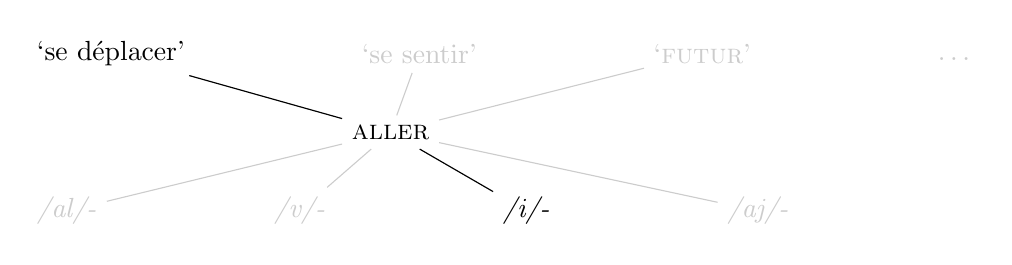
\begin{tikzpicture}
 \graph [grow down, branch right sep=2cm,edges=black!20,nodes=black!20] 
   {
     {‘se déplacer’ [black], ‘se sentir’, futur/‘\textsc{futur}’}
     -- {ALLER/\textsc{aller} [black,xshift=4cm]}
     -- {al/\textit{/al/-}, v/\textit{/v/-}, i/\textit{/i/-} [black], aj/\textit{\strut/aj/-}
     };
     {[edges=black]‘se déplacer’ -- ALLER -- i};
     {[grow right] futur -!- dots/{\strut …}};
   };
\end{tikzpicture}
\caption{Signe\label{fig:}}
\end{figure}

\begin{figure}
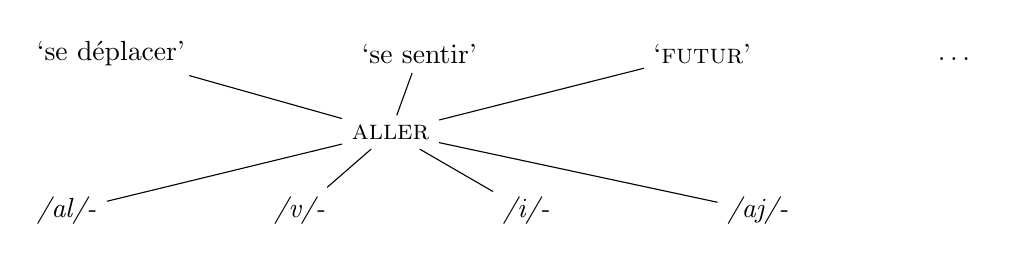
\begin{tikzpicture}
 \graph [grow down, branch right sep=2cm] 
   {
     {‘se déplacer’, ‘se sentir’, futur/‘\textsc{futur}’}
     -- {ALLER/\textsc{aller} [black,xshift=4cm]}
     -- {al/\textit{/al/-}, v/\textit{/v/-}, i/\textit{/i/-}, aj/\textit{\strut/aj/-}
     };
     {[grow right] futur -!- dots/{\strut …}};
   };
\end{tikzpicture}
\caption{Signème}
\end{figure}

La symétrie entre sens et forme n’est pas complète. Le locuteur fait le choix d’un sens et ce choix peut se porter sur n’importe lequel des signifiés du syntaxème. Mais le «~choix~» du signifiant n’en est pas un : il est \textbf{totalement imposé par l’environnement}, c’est-à-dire par les choix adjacents du locuteur. Dans le cas de \textsc{aller}, le «~choix~» du signifiant est conditionné par la flexion et donc par le choix du temps et celui du sujet via l’accord.

Nous montrons pour finir le découpage du syntaxème selon la forme, qui nous donne les (allo)morphes, et le découpage selon le sens, qui nous donne les acceptions.

\begin{figure}
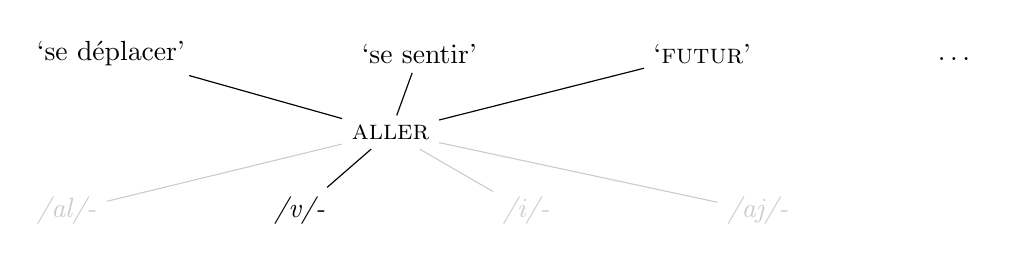
\begin{tikzpicture}
 \graph [grow down, branch right sep=2cm,edges=black!20,nodes=black!20] 
   {
     {‘se déplacer’ [black], ‘se sentir’ [black], futur/‘\textsc{futur}’ [black]}
     -- {ALLER/\textsc{aller} [black,xshift=4cm]}
     -- {al/\textit{/al/-}, v/\textit{/v/-} [black], i/\textit{/i/-} , aj/\textit{\strut/aj/-}
     };
     {[edges=black] {‘se déplacer’, ‘se sentir’, futur} -- ALLER -- v};
     {[grow right] futur -!- dots/{\strut …} [black]};
   };
\end{tikzpicture}
    \caption{(Allo)morphe}             
\end{figure}
           
\begin{figure}
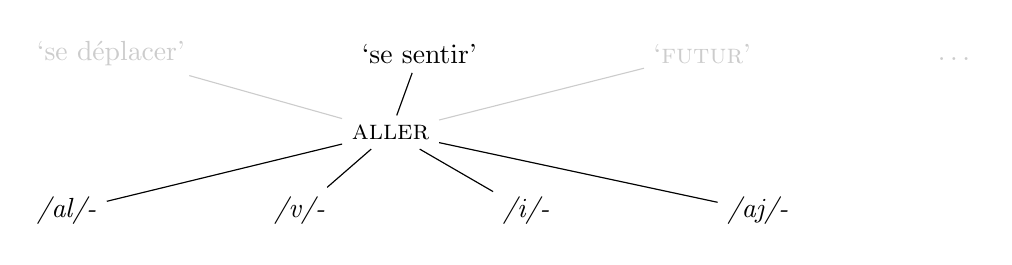
\begin{tikzpicture}
 \graph [grow down, branch right sep=2cm,edges=black!20,nodes=black!20] 
   {
     {‘se déplacer’, ‘se sentir’ [black], futur/‘\textsc{futur}’}
     -- {ALLER/\textsc{aller} [black,xshift=4cm]}
     -- {[nodes=black] al/\textit{/al/-}, v/\textit{/v/-}, i/\textit{/i/-} , aj/\textit{\strut/aj/-}
     };
     {[edges=black] {‘se sentir’} -- ALLER -- {al, v, i , aj}};
     {[grow right] futur -!- dots/{\strut …}};
   };
\end{tikzpicture}
    \caption{Acception}
\end{figure}

Il devient alors possible de voir le syntaxème comme un niveau d’articulation entre sens et forme. On peut ainsi scinder la correspondance sens-forme en deux modules et voir les sémantèmes et les morphèmes comme les éléments respectifs de ces deux modules :

\begin{figure}
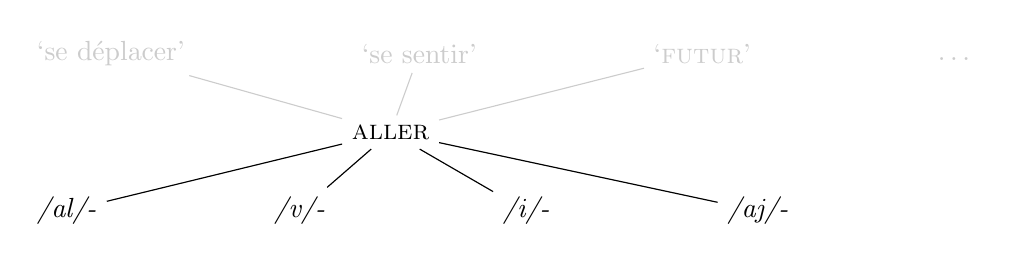
\begin{tikzpicture}
 \graph [grow down, branch right sep=2cm,edges=black!20,nodes=black!20] 
   {
     {‘se déplacer’, ‘se sentir’, futur/‘\textsc{futur}’}
     -- {ALLER/\textsc{aller} [black,xshift=4cm]}
     -- {al/\textit{/al/-} [black], v/\textit{/v/-} [black], i/\textit{/i/-} [black], aj/\textit{\strut/aj/-} [black]};
     {[edges=black] ALLER -- {al/\textit{/al/-} [black], v/\textit{/v/-} [black], i/\textit{/i/-} [black], aj/\textit{\strut/aj/-} [black]}};
     {[grow right] futur -!- dots/{\strut …}};
   };
\end{tikzpicture}
\caption{Morphème\label{fig:}}
\end{figure}

\begin{figure}
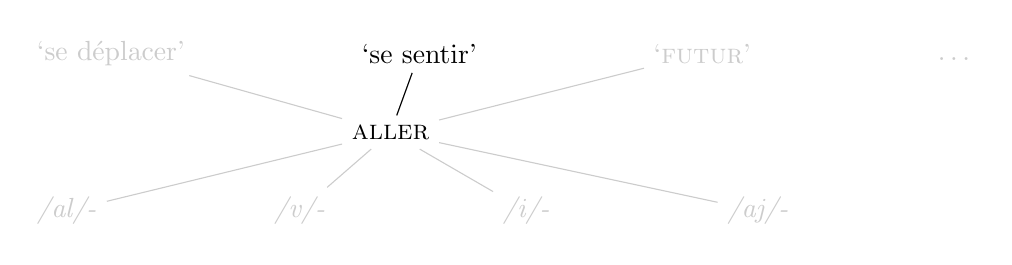
\begin{tikzpicture}
 \graph [grow down, branch right sep=2cm,edges=black!20,nodes=black!20] 
   {
     {‘se déplacer’, ‘se sentir’ [black], futur/‘\textsc{futur}’}
     -- {ALLER/\textsc{aller} [black,xshift=4cm]}
     -- {al/\textit{/al/-}, v/\textit{/v/-}, i/\textit{/i/-}, aj/\textit{\strut/aj/-}};
     {[edges=black] ALLER -- {‘se sentir’ [black]}};
     {[grow right] futur -!- dots/{\strut …}};
   };
\end{tikzpicture}
\caption{Sémantème}    
\end{figure}

En d’autres termes, on peut voir les morphes et morphèmes comme des (ensembles de) \textstyleTermes{demi-signes de surface} dont le signifié est un élément abstrait (représenté par le nom de lexème \textsc{aller} dans nos figures), qui sert lui même de signifiant aux \textstyleTermes{demi-signes profonds} que sont les sémantèmes. Travailler avec des demi-signes est particulièrement intéressant quand on considère des locutions : on peut en effet considérer que le signifiant de sémantèmes complexes comme $⌜$\textsc{àvoir} \textsc{les} \textsc{pieds} \textsc{sur} \textsc{terre}$⌝$ ou comme le passé composé sont des configurations de syntaxèmes.

\loupe{Signèmes et signes : unités de la langue et unités de la parole}{%\label{sec:2.3.18}
    Depuis les travaux de Saussure, la quasi-totalité des ouvrages de linguistique considèrent que les unités de la langue sont des signes. Ce n’est pas notre cas. Nous considérons que les unités de la langue, celles qui sont dans notre cerveau, sont plutôt des signèmes, c’est-à-dire des \textbf{faisceaux de correspondances entre sens et formes}. Lorsqu’un locuteur produit un énoncé, il choisit de tels faisceaux qu’il assemble. Un signème donné est choisi parce que l’un des sens du signème est un sens que le locuteur veut exprimer. Par exemple, si le locuteur veut parler d’un de ses prochains déplacements, il pourra choisir le faisceau \textsc{aller} et produire un énoncé comme «~\textit{Je vais à Paris la semaine prochaine.}~» Le choix de la forme \textit{v-} du faisceau lui est imposé par le contexte : ce sont les sens ‘moi’ réalisé par \textit{je} et ‘\textsc{présent}’ qui vont sélectionner l’allomorphe \textit{v-} parmi les différents morphes de \textsc{aller}. Ce «~choix~» du signifiant est totalement indépendant du sens par lequel le locuteur a sélectionné le signème \textsc{aller}.

    On peut donc dire que ce ne sont pas les signes qui sont organisés en faisceau, mais \textbf{les faisceaux} qui \textbf{se réalisent par des signes en parole}. Lorsqu’un signème est utilisé dans un énoncé, c’est forcément qu’il a été choisi pour un de ses sens et qu’il est réalisé sous une de ses formes. Donc, dans un énoncé, le signème apparaît sous la forme d’un signe. Selon nous, c’est bien un signème qui a été sélectionné dans notre cerveau et c’est par l’intermédiaire de ce faisceau qu’un signe a été réalisé. En reprenant la terminologie saussurienne, on peut dire que les \textbf{signèmes} sont les \textbf{unités de la langue} et les \textbf{signes} les \textbf{unités de la parole}.

    Il faut aussi noter que les signes sont quasiment des observables : on peut dans un texte repérer leur signifiant et mesurer leur contribution sémantique. Les signèmes, eux, sont des constructions théoriques. Leur existence ne peut être prouvée qu’au sein du modèle (tant qu’on n’a pas les moyens de les observer au sein du cerveau).
}
\section{Autonomie de la syntaxe et de la sémantique}\label{sec:2.3.19}

Nous allons conclure ce chapitre en soulignant un point fondamental concernant les unités sémantiques et la syntaxe : le comportement des syntaxèmes (c’est-à-dire leur combinatoire libre avec d’autres syntaxèmes, leur placement ou leur schéma prosodique) dépend assez peu des unités sémantiques auxquelles ils appartiennent. Par exemple, si l’on prend les occurrences de \textsc{prendre} dans n’importe quel phrasème dont il est la tête ($⌜$\textsc{prendre} \textsc{les} \textsc{jambes} \textsc{à} \textsc{son} \textsc{cou}$⌝$, $⌜$\textsc{prendre} \textsc{son} \textsc{pied}$⌝$, $⌜$\textsc{s’en} \textsc{prendre} \textsc{plein} \textsc{la} \textsc{gueule}$⌝$, etc.), \textsc{prendre} y conserve ses propriété habituelles de verbe, prend une flexion verbale, et peut-être modifié par les mêmes types d’éléments (adverbes, etc.). Ses compléments ne peuvent pas être modifiés (c’est l’effet du figement), mais ils se placent comme des compléments libres et obéissent aux mêmes règles de phonétisation (prosodie comprise).

En général, les phrasèmes ont tendance à avoir une combinatoire plus restreinte et à supporter moins facilement les manipulations que les combinaisons libres, mais ce n’est pas une règle. Par exemple, si on compare le sémantème $⌜$\textsc{briser} \textsc{la} \textsc{glace}$⌝$ ‘dissiper la gêne’ avec la combinaison libre \textsc{briser} \textsc{${\oplus}$ glace}, on voit que les deux combinaisons acceptent d’entrer dans des constructions analogues : négation (\textit{Pierre n’a pas brisé la glace}), clivage du sujet \textit{(C’est Pierre qui a brisé la glace le premier}) ou passif (\textit{La glace a été brisée}). Par contre, le clivage de l’objet (\textit{C’est la glace que Pierre a brisé}) n’est possible qu’avec la combinaison libre, c’est-à-dire quand l’objet est une unité sémantique. Le comportement des phrasèmes dépend donc fortement du comportement des syntaxèmes qui les composent, alors que celui des syntaxèmes est relativement indépendant du fait qu’il forme un sémantème ou sont seulement une composante d’un phrasème.

Morphèmes et sémantèmes structurent le lexique de la langue : ce sont respectivement les plus petites et les plus grandes unités minimales de première articulation. Cependant, le fait que les unités minimales du point de vue du signifiant (les morphèmes) ne correspondent pas aux unités minimales du point de vue du signifié (les sémantèmes) entraine que ni les unes, ni les autres ne sont les unités de la syntaxe. Nous allons donc pouvoir maintenant présenter les unités de la syntaxe et cette mise au point sur morphèmes et sémantèmes permettra, nous l’espérons, de bien comprendre ce qui est et n’est pas une unité de la syntaxe.

\exercices{%\label{sec:2.3.20}
    \exercice{1} Étudier le caractère motivé ou non des signifiants des signes désignant les nombres de \textit{dix} à \textit{vingt}.

    \exercice{2} Alors que la grammaire normative indique que le verbe \textsc{pallier} doit être utilisé transitivement (\textit{pallier un problème}), de nombreux locuteurs produisent aujourd’hui \textit{pallier à un problème}. Qu’est-ce qui peut expliquer que la construction de ce verbe change de cette façon ? Qu'est-ce qui permet qu'une construction puisse changer ?

    \exercice{3} L’énoncé «~\textit{Si j’étais toi, je demanderais à} \textbf{\textit{ma}} \textit{mère.}~» est ambigu : \textit{ma mère} peut référer à la mère du locuteur ou à celle de l’interlocuteur. Cela remet-il en question une analyse purement déictique du pronom \textsc{moi~}? Quelle solution proposer ?

    \exercice{4}
    \begin{enumerate}[label=\alph*.]
    \item Montrer que \textit{grièvement blessé} est une collocation.

    \item L’adverbe \textit{grièvement} joue un rôle d’intensifieur auprès de \textit{blessé}. Chercher d’autres exemples d’intensifieurs exprimés par un collocatif pour des adjectifs, mais aussi pour des verbes et des noms.
    \end{enumerate}

    \exercice{5} Identifier les phrasèmes et les collocations des phrases suivantes :

    \begin{enumerate}
    \item  \textit{L’agent de police dormait à poings fermés.}
    \item  \textit{Il est allé faire la sieste sur la plage.}
    \item  \textit{Je ne peux pas le piffrer.}
    \item  \textit{Il a je ne sais quelle idée en tête.}
    \end{enumerate}

    \exercice{6} Déterminer parmi les occurrences suivantes du lexème \textsc{table} différentes acceptions. Pour chacune d’elle vous indiquerez si elle appartient à un phrasème ou à une collocation.
    \begin{enumerate}
    \item  \textit{Cette table a un pied central.}
    \item  \textit{On passera à table à midi.}
    \item  \textit{Tu as intérêt à te mettre à table rapidement si tu ne veux pas te retrouver en tôle.}
    \item  \textit{Consulter la table des matières en début d’ouvrage.}
    \item  \textit{On vous a réservé la meilleure table.}
    \item  \textit{Le résultat est dans la table de la page précédente.}
    \end{enumerate}

    \exercice{7} Un syntaxème comme \textsc{blanc} peut être utilisé dans la formation de différentes expressions : \textit{voter blanc, blanc comme un linge, blanc comme neige, blanchir le linge, blanchisserie}. Quelles composantes du signe sont affectées dans ces différents emplois ?
}
\lecturesadditionnelles{%\label{sec:2.3.21}
    Le \textbf{sémantème}, appelé \textit{monème} par André Martinet, est défini dans ses \textit{Éléments de linguistique générale}, dont on consultera les sections 1 à 19 du chapitre 1 et le chapitre 4. Les notions introduites par Martinet sont également présentées dans l'ouvrage de Denis Cosatouec et Françoise Guérin. Le chapitre sur \textit{Les unités significatives} de l’encyclopédie d'Oswald Ducrot et jean-Marie Schaeffer complètera cette lecture.

    La syntaxe des \textbf{locutions} est étudiée en détail dans la thèse de Marie-Sophie Pausé. La distinction entre \textbf{transparence} et \textbf{diagrammaticité} (appelée \textit{analycité}) est bien dégagée dans un article de Marie Helena Svensson de 2008.

    Le \textbf{découpage paradigmatique} en unités lexicales ainsi que les \textbf{collocations} sont très bien présentés dans l'ouvrage de lexicologie d'Alain Polguère. Voir également l'\textit{Introduction à la lexicologie explicative et combinatoire} co-écrite avec Igor Mel’čuk pour une introduction plus technique aux \textbf{fonctions lexicales}, ainsi que le \textit{Lexique actif du français} pour des exemples d’entrées lexicales avec leurs collocatifs. Les \textbf{collocations morphologiques} sont présentées dans un article de David Beck de 2019.

    La notion de \textbf{faisceau de signes} est introduite dans le premier tome du \textit{Cours de Morphologie Générale} d'Igor Mel’čuk (voir \chapref{sec:2.1}) lors de la description des grammèmes (p. 278), mais n'est pas exploitée pour les syntaxèmes en général. Les grammèmes chez Mel’čuk n'ont d'ailleurs pas un statut de signe linguistique.

    \FurtherReading{2-3}
}
\corrections{%\label{sec:2.3.22}
    \corrigé{1} Les nombres \textit{dix-sept, dix-huit} et \textit{dix-neuf} sont construits selon la syntaxe régulière des nombres (comme \textit{cent vingt-huit} par exemple). On peut donc considérer qu’ils sont compositionnels. Les nombres \textit{onze, douze, treize, quatorze, quinze, seize} ne sont pas décomposables en synchronie, même s’ils possèdent tous une terminaison en \textit{{}-ze} et un radical en partie transparent. Ils sont donc assez motivés. Les signifants des nombres \textit{dix} et \textit{vingt} sont eux totalement arbitraires.

    \corrigé{2} Il semble que le verbe \textsc{pallier} ait changé de construction en raison de sa proximité sémantique avec \textsc{remédier} ou $⌜$\textsc{s’attaquer}$⌝$ qui se construisent avec X V \textit{à} Y. Le fait qu’un verbe puisse changer de construction montre bien qu’il y a une certaine indépendance de la construction par rapport au lexème lui-même. Voir l’\encadref{fig:2.3.4} \textit{Constructions verbales et accords : signes vides} ?.

    \corrigé{3} Le pronom \textsc{moi} ne réfère pas forcément au locuteur à proprement parler, mais à celui à qui on attribue les paroles. C’est le cas avec le discours rapporté : \textit{Zoé m’a dit : «~Je viendrai~».} C’est aussi le cas ici, où il y a un transfert du ‘toi’ au ‘moi’.

    \corrigé{4} L’adverbe \textsc{grièvement} ne peut modifier que l’adjectif \textsc{blessé}. \textsc{blessé} garde son sens usuel et \textsc{grièvement} fonctionne comme un intensifieur. L’absence de commutation possible sur \textsc{blessé} montre que \textsc{grièvement} est un collocatif. Le choix de \textsc{blessé} est libre et le choix de \textsc{grièvement} est dépendant de ce premier choix. Les intensifieurs sont les plus productifs des collocatifs. En voici quelques uns : \textit{gravement malade, con comme un balai, armé jusqu’au dent, aimer à la folie, applaudir des deux mains, craindre comme la peste, grand ami, gros fumeur, augmentation substantielle, catastrophe épouvantable, désaccord profond, bataille sans merci, forme olympique,} etc.

    \corrigé{5}
    \begin{enumerate}
    \item  Une expression comme \textit{agent de police} se situe à la frontière entre collocation et phrasème. On peut la considérer comme une collocation non standard de base \textsc{police}, le collocatif \textsc{agent} désignant l'un des types de fonctionnaire travaillant à la police. Néanmoins, \textsc{police} parait peu modifiable et il est loin d'être certain que \textsc{agent} soit choisi à partir du choix initial de \textsc{police}. (Le problème est encore compliqué ici par le fait qu’il y a une autre acception de \textsc{agent} qui à elle seule veut dire ‘agent de police’.) \textrm{$⌜$}\textsc{à} \textsc{poings} \textsc{fermés}\textrm{$⌝$} est également un phrasème et ce phrasème est un collocatif de \textsc{dormir} marquant l’intensification.
    \item  \textit{faire la sieste} est un exemple typique de construction à verbe support, où la base \textsc{sieste} est un nom prédicatif et le collocatif \textsc{faire} n’a pas de contribution propre. Il y a une autre collocation moins évidente qui est \textit{sur la plage}. En effet, la préposition locative \textsc{sur} n’est pas totalement prédictible : on peut dire \textit{à/sur la plage}, mais, par exemple, on doit dire \textit{à/dans la campagne} et seulement \textit{dans la forêt.} On considère donc que les prépositions locatives sont des collocatifs dont le choix est restreint par le nom qui suit.
    \item  Le verbe \textsc{piffrer} ne s’utilise que précédé de \textsc{pouvoir} (*\textit{je ne le piffre pas}) et~dans un contexte négatif (*\textit{je peux le piffrer}). Par contre, différentes réalisation de la négation sont possibles : \textit{je n’ai jamais pu le piffrer} ; \textit{personne ne peux le piffrer}. On a donc un phrasème que nous notons \textrm{$⌜$}\textsc{(ne} \textsc{pas)} \textsc{pouvoir} \textsc{piffrer}\textrm{$⌝$} (la parenthèse indique qu’une autre négation peut remplacer \textsc{ne} \textsc{pas}).
    \item  Comme dans les cas précédent, on voit si des commutations sont possibles. On remarque d’abord que le déterminant de \textsc{idée} peut être changé : \textit{avoir une idée en tête}. De plus, \textsc{idée} peut commuter avec d’autres noms : \textit{avoir un problème/une musique en tête.} Ou même un pronom : \textit{avoir quelque chose en tête}. Il nous reste donc l’expression \textit{avoir N en tête}. Or on peut encore commuter le verbe : \textit{on m’a mis cette idée en tête}, \textit{avec ça en tête}. Au final, on a un phrasème \textrm{$⌜$}\textsc{en} \textsc{tête}\textrm{$⌝$} dont \textsc{avoir} est un collocatif (un verbe support). Quant au déterminant \textit{je ne sais quel}, il appartient à un paradigme de pronom : \textit{je ne sais qui/quoi/où/comment}. L’élément \textit{je ne sais} possède lui-même une certaine variabilité : \textit{on ne sait quel, Dieu sait quel}. Au final, on considérera quand même que \textrm{$⌜$}\textsc{je} \textsc{ne} \textsc{sais} \textsc{quel}\textrm{$⌝$} est un phrasème, mais cet exemple montre qu’il y a plusieurs degrés de décompositionalité et que la frontière entre phrasème et syntagme compositionnel n’est pas parfaitement nette.
    \end{enumerate}

    \corrigé{6} Le lexème \textsc{table} est un sémantème dans les exemples 1, 5 et 6. Il s’agit de trois acceptions différentes, puisque \textsc{table} désigne un meuble en 1, un lieu gastronomique en 5 et un type de diagramme en 6. En 2, on a une locution \textrm{$⌜$}\textsc{à} \textsc{table}\textrm{$⌝$}, comme le montre l’absence de commutation possible sur \textsc{table}. Par contre, \textsc{passer}, qui peut commuter avec \textrm{$⌜$}\textsc{se} \textsc{mettre}\textrm{$⌝$} ou \textsc{être}, est un collocatif de \textrm{$⌜$}\textsc{à} \textsc{table}\textrm{$⌝$}. En 3, la commutation de \textrm{$⌜$}\textsc{se} \textsc{mettre}\textrm{$⌝$} avec \textsc{être} n’est plus possible et \textrm{$⌜$}\textsc{se} \textsc{mettre} \textsc{à} \textsc{table}\textrm{$⌝$} forme une locution signifiant ‘passer des aveux’. En 4, \textrm{$⌜$}\textsc{table} \textsc{des} \textsc{matières}\textrm{$⌝$} est également un phrasème. En 5, \textsc{table} est la base de deux collocations : \textsc{réserver} est un collocatif exprimant une étape préliminaire à l'utilisation de la table, tandis que \textsc{bon} (ici sous la forme superlative \textit{meilleur}) est un collocatif intensifiant la qualité de la table. En 6, \textsc{table} est associé au collocatif \textsc{dans}, qui est une préposition exprimant la localisation. On notera que les autres acceptions de \textsc{table}, utilisées en 1 et 5, ne pourraient pas s'utiliser avec cette préposition.

    \corrigé{7} Dans \textit{voter blanc}, \textsc{blanc} est un collocatif de \textsc{voter}. Dans ce contexte, \textsc{blanc} signifie ‘en mettant un bulletin blanc’. Dans \textit{blanc comme un linge}, c’est \textrm{$⌜$}\textsc{comme} \textsc{un} \textsc{linge}\textrm{$⌝$} qui est un collocatif de \textsc{blanc}, mais \textsc{blanc} a une acception particulière ‘qui manifeste un sentiment de peur ou de colère’. Par contre, \textrm{$⌜$}\textsc{blanc} \textsc{comme} \textsc{neige}\textrm{$⌝$} est un phrasème, car \textsc{blanc} seul ne peut avoir le sens ‘sans aucune preuve à charge’ ; \textsc{blanc} y est donc désémantisé, puisque le sens est porté par la locution complète. Dans \textsc{blanchir,} le radical /blāʃ/ est le même morphème que le syntaxème \textsc{blanc}, mais cette acception n’a plus du tout le même syntactique (il s’agit d’un conversion de nom en verbe) et son signifié est également modifié et est devenu ‘laver à haute température pour rendre blanc et pur’. \textsc{blanchisserie} est construit à partir de \textsc{blanchir}, mais le signe a subi une nouvelle désyntactisation et désémantisation, puisque même si \textsc{blanchisserie} est assez diagrammatique, il n’est pas compositionnel pour autant.
}


\part{Structures syntaxiques et topologique~:\\Comment les unités se combinent}\label{sec:3}
\section*{Présentation}

Cette troisième partie est consacrée à la façon dont les signes linguistiques se combinent pour former des syntagmes et aux structures qui en découlent. Le \chapref{sec:3.1}, où nous donnons notre définition de la syntaxe, est consacré à distinguer l’unité minimale de la syntaxe, le syntaxème, du syntagme. Le \chapref{sec:3.2} introduit la structure de connexion en montrant comment la combinaison des unités syntaxiques définit un ensemble de connexions qui forment la charpente de la structure syntaxique. Le \chapref{sec:3.3} montre que cette structure est hiérarchique en introduisant les notions de tête et de dépendance. Le \chapref{sec:3.4} étudie les équivalences et différences entre les structure de dépendance, qui mettent en avant les relation syntagmatiques entre unités, et les arbres de constituants, qui mettent en avant les relations d’enchâssement entre les unités. Le \chapref{sec:3.5} étudie l’ordre des mots et la façon dont les syntaxèmes se regroupent lorsqu’ils sont dans l’ordre linéaire, définissant ainsi ce que nous appelons la structure topologique. Le \chapref{sec:13}, à venir, présente la structure qui rend compte de la combinaison des sémantèmes et les distorsions avec les structures qui rendent compte de la combinaison des syntaxèmes. 

\chapter{\gkchapter{Syntaxèmes et syntagmes}{La délimitation des unités minimales de la syntaxe}}\label{sec:3.1}

\section{Syntaxème, morphème et sémantème}\label{sec:3.1.0}\largerpage

Nous avons donné une première définition du syntaxème dans la partie~\ref{sec:2}. L’objectif de ce chapitre est de donner une définition plus précise du syntaxème, de préciser la frontière entre le syntaxème et le syntagme, qui est une combinaison de syntaxèmes, et de donner une définition de ce que nous appelons la syntaxe.

Rappelons que nous appelons \hi{morphèmes} les signes minimaux du point de vue de la forme (\chapref{sec:2.2}) et \hi{sémantèmes} les signes minimaux du point de vue du sens (\chapref{sec:2.3}). D’où vient la nécessité de considérer, en plus de ces deux unités, les unités que nous appelons les \hi{syntaxèmes~}?

Le signe idéal est un \hi{sémantème simple}, c’est-à-dire une unité minimale de forme et de sens, un sémantème qui est aussi un morphème. (Nous devrions dire «~un sémantème qui est une acception d’un morphème~», car la quasi-totalité des morphèmes ont plusieurs acceptions.) Comme on l’a vu au \chapref{sec:2.3}, il n’y a pas de correspondance entre unités minimales de sens et unités minimales de forme et un grand nombre de sémantèmes sont complexes, c’est-à-dire sont la combinaison de plusieurs morphèmes. Il convient néanmoins de distinguer, parmi les sémantèmes complexes, ceux qui se comportent comme des sémantèmes simples et ceux qui se comportent plutôt comme une combinaison de sémantèmes simples. Ce sont les premiers que nous appelons des syntaxèmes.

Nous avons déjà donné, dans le \chapref{sec:2.1}, l’exemple des sémantèmes \textsc{décapsuleur} et $⌜$\textsc{avoir} \textsc{les} \textsc{pieds} \textsc{sur} \textsc{terre}$⌝$. Les deux sont composés de plusieurs morphèmes, mais, alors que \textsc{décapsuleur} se comporte comme un sémantème simple – comme \textsc{bol} ou \textsc{couteau} –, $⌜$\textsc{avoir} \textsc{les} \textsc{pieds} \textsc{sur} \textsc{terre}$⌝$ ne se comporte pas comme un verbe simple. En fait, $⌜$\textsc{avoir} \textsc{les} \textsc{pieds} \textsc{sur} \textsc{terre}$⌝$ se comporte comme la combinaison libre \textit{avoir les mains sur la table} et est construit de manière \hi{analogue} à cette expression par la combinaison du verbe \textsc{avoir} et de compléments avec lesquels il s’est figé sémantiquement. À l’inverse, \textsc{décapsuleur} n’est pas construit de manière analogue à une expression libre.

\section{Analogie structurelle}\label{sec:3.1.2}

La notion d’analogie (structurelle) joue un rôle central dans la définition des unités syntaxiques. Voici comment nous la définissons.

\Definition{\terme{analogie (structurelle)}}
{Une combinaison de signes A+B est dite (\notextstyleTermes{structurellement}) \notextstyleTermes{analogue} à une combinaison A’+B’ si A a une distribution équivalente à A’, B à B’ et A+B à A’+B’.}

\begin{sloppypar}
Cette définition va être illustrée dans la \sectref{sec:3.1.4}. Donnons avant cela quelques autres définitions basées sur l’analogie, à commencer par la définition du syntagme.
\end{sloppypar}

\Definition{\textstyleTermes{syntagme}}
{Un \textstyleTermes{syntagme} est une combinaison de signes \hi{structurellement analogue} à une \hi{combinaison libre}.}

En incluant les combinaisons \textit{analogues} à des combinaisons libres, nous incluons les constructions figées, c’est-à-dire la possibilité qu’un syntagme ne soit pas une combinaison libre, mais se comporte syntaxiquement comme une combinaison libre.

Les syntagmes sont des combinaisons régulières de signes du point de vue de leur \hi{syntactique} (voir la \sectref{sec:2.1.3} sur \textit{Signifié, syntactique, signifiant}). Autrement dit, A+B forme un syntagme si le syntactique de A+B se calcule de manière régulière à partir des syntactiques de A et de B. Mais la combinaison des signifiants de A et B peut être irrégulière (par exemple être un amalgame comme \textit{au} = \textit{à}\,$\oplus$\,\textit{le} ou \textit{viens} = \textsc{venir}\,$\oplus$\,indicatif\,$\oplus$\,présent\,$\oplus$\,2\,$\oplus$\,singulier) ou la combinaison des signifiés de A et B peut être irrégulière (lorsque A+B est une locution).

La notion de syntaxème peut maintenant être définie de manière plus rigoureuse.

Par définition, tout syntagme X est une combinaison A+B qui est libre ou analogue à une combinaison libre. On peut donc décomposer X en deux signes A et B et une telle \notextstyleTermes{décomposition} est dite \notextstyleTermes{syntaxique}\is{décomposition syntaxique}. Nous opposons une telle décomposition à une \notextstyleTermes{décomposition morphologique}, qui serait une décomposition en morphèmes reposant uniquement sur la commutation propre.

La décomposition syntaxique peut être appliquée récursivement. Si les signes A et B sont à nouveau des syntagmes, on pourra les décomposer en deux signes et ainsi de suite, jusqu’à ce qu’on arrive à des signes qui ne peuvent plus être décomposés selon ce principe. C’est ce que nous appelons des \notextstyleTermes{syntaxèmes}\is{syntaxème}.

Toute combinaison de deux syntaxèmes est un syntagme et tout syntagme est une combinaison de plusieurs syntaxèmes. Plus généralement :

\Definition{\textstyleTermes{unité syntaxique}}
{Les \notextstyleTermes{unités syntaxiques} sont \hi{les signes qui commutent librement} dans leur contexte ou qui sont analogues à de tels signes.}

Une unité syntaxique est soit un \hi{syntagme}, soit un \hi{syntaxème}. Et donc :\largerpage

\Definition{\textstyleTermes{syntaxème}}
{Les \notextstyleTermes{syntaxèmes} sont donc les \hi{unités syntaxiques minimales}. Un syntaxème est \hi{indécomposable en deux unités syntaxiques}.}

\eiffel[sec:3.1.3]{Le collimateur et la sellette}{%
    En général, tout syntaxème commute librement dans certains environnements, mais il existe des cas extrêmes comme \textsc{fur}, qui n’apparaît que dans le \is{figement}\is{phrasème}phrasème $⌜$\textsc{au} \textsc{fur} \textsc{et} \textsc{à} \textsc{mesure}\textrm{$⌝$}. Le fait que \textit{au fur} soit assez clairement analogue à une combinaison libre, en raison notamment de la coordination avec \textit{à mesure}, amène à considérer \textit{fur} comme un syntaxème. Les éléments lexicaux qui ne s’utilisent plus (guère) que dans des phrasèmes sont quand même assez nombreux : (\textit{être}) \textit{aux} \textbf{\textit{aguets}}, (\textit{avancer}) \textit{à la queue} \textbf{\textit{leu leu}}, \textit{à l’}\textbf{\textit{instar}} \textit{de,} (\textit{utiliser qqch}) \textit{à bon/mauvais} \textbf{\textit{escient}}, (\textit{poser une question}) \textit{à brûle-}\textbf{\textit{pourpoint}}, (\textit{rouler}) \textit{à toute} \textbf{\textit{blinde}}, (\textit{aller}) \textit{au diable} \textbf{\textit{vauvert}}, (\textit{avoir qqn}) \textit{dans le} \textbf{\textit{collimateur}}, \textit{de plein} \textbf{\textit{gré}}, (\textit{coeur}) \textit{battre la} \textbf{\textit{chamade}}, \textit{faire de la} \textbf{\textit{charpie}} (\textit{de qqch}), \textit{de} \textbf{\textit{bric}} \textit{et de} \textbf{\textit{broc}}, \textit{de} \textbf{\textit{guingois}}, \textit{de} \textbf{\textit{traviole}}, \textit{en} \textbf{\textit{catimini}}, \textit{en} \textbf{\textit{filigrane}}, \textit{mettre la} \textbf{\textit{sourdine}}, \textit{en un} \textbf{\textit{tournemain}}, \textit{en} \textbf{\textit{vrac}}, \textit{et tout le} \textbf{\textit{bastringue}}, \textit{manger à tous les} \textbf{\textit{râteliers}}, (\textit{mettre qqn}) \textit{sur la} \textbf{\textit{sellette}}, \textit{passer au} \textbf{\textit{crible}}, \textit{prendre la poudre d’}\textbf{\textit{escampette}}, \textit{sans coup} \textbf{\textit{férir}}, \textit{sans} \textbf{\textit{encombre}}, \textit{se faire du} \textbf{\textit{mouron}} (\textit{pour qqn}), \textit{s’en soucier comme d’une} \textbf{\textit{guigne}}, \textit{sonner le} \textbf{\textit{glas}} (\textit{de qqch}), \textit{tailler des} \textbf{\textit{croupières}} (\textit{à qqn}), (\textit{mettre}) \textit{en} \textbf{\textit{exergue}}, \textit{tous} \textbf{\textit{azimuts}}, etc.
}
\section{Syntagme ou syntaxème ?}\label{sec:3.1.4}

Nous allons mettre en pratique nos définitions en étudiant des unités qui sont à la limite entre syntagme et syntaxème.

Commençons en comparant les expressions verbales figées $⌜$\textsc{s’en} \textsc{aller}$⌝$ et $⌜$\textsc{s’enfuir}$⌝$. Dans, les deux expressions, le morphème \textit{en} est à l’origine la cliticisation d’un complément délocatif du type \textit{de quelque part} : \textit{fuir de quelque part~}→ \textit{en fuir}. Il n’y a pas de différence au niveau du figement sémantique entre ces deux expressions. Pourtant elles sont orthographiées différemment et à juste titre. La question est de savoir si les combinaisons \textit{en} + \textit{aller} et \textit{en} + \textit{fuir} se comportent comme un verbe simple ou comme une combinaison libre clitique \textsc{en} ${\oplus}$ Verbe du genre \textit{en partir} (\textit{partir de quelque part}). Nous allons appliquer la définition de l’analogie structurelle (\sectref{sec:3.1.2}) avec A = A’ = \textit{en}, B = \textit{fuir}/\textit{aller} et B’ = \textit{partir}. Il faut chercher les situations où le clitique \textsc{en} ne se comporte pas de la même façon qu’un préfixe \textit{en-}. Il n’y en a que deux : la combinaison avec un auxiliaire qui viendra séparer le clitique et le verbe (\textit{j’}\textbf{\textit{en}} \textit{suis} \textbf{\textit{parti}}) et l’impératif qui inverse l’ordre (\textit{Pars-en} !). On voit que pour $⌜$\textsc{s’enfuir}$⌝$, \textit{en-} se comporte bien comme un affixe en restant solidaire du radical (\textit{je me suis enfui} ; \textit{Enfuis-toi} !), mais que $⌜$\textsc{s’en} \textsc{aller}$⌝$ se comporte encore comme une combinaison \textsc{en} ${\oplus}$ Verbe (\textit{je m’en suis allé~}; \textit{Va-t-en} !). On note quand même que la forme \textit{je m’en suis allé} apparaît comme très soutenue (voire archaïque) et que, dans un style relâché, on pourra avoir~\textsuperscript{?}\textit{je me suis en allé}, les locuteurs évitant au final de produire l’une ou l’autre des formes. En conclusion, \textit{enfuir} est un seul syntaxème, tandis qu’\textit{en aller} est encore la combinaison de deux syntaxèmes, c’est-à-dire un syntagme.

\begin{sloppypar}
Un autre exemple est celui de \textsc{bonhomme} et $⌜$\textsc{bonne} \textsc{femme}$⌝$. Ici, on a deux combinaisons Adjectif + Nom qui se sont figées. Les conventions orthographiques veulent qu’on écrive \textsc{bonhomme} en un seul mot, bien que pour son pluriel \textit{bonshommes}, il soit possible de faire la liaison (/\textstylePhono{b\~{ɔ}zɔm}/), tandis que $⌜$\textsc{bonne} \textsc{femme}$⌝$ s’écrit en deux mots. Voyons comme précédemment si cette différence d’orthographe est bien motivée. Il s’agit donc de savoir si ces deux sémantèmes se comportent comme un nom simple ou comme une combinaison libre Adjectif ${\oplus}$ Nom telle que \textit{bonne orange}. Cela ne sera possible que s’il existe une différence distributionnelle entre le nom et la combinaison Adjectif ${\oplus}$ Nom. Une telle différence existe bien : le déterminant indéfini pluriel \textsc{des} possède une forme faible \textit{de} qui s’utilise devant un adjectif, tandis que la forme \textit{des} est obligatoire devant un nom (\textit{Pierre a acheté} \textbf{\textit{des}} \textit{oranges} vs \textit{Pierre a acheté} \textbf{\textit{de}} \textit{bonnes oranges}). Or l’énoncé \textit{\textsuperscript{\#}}\textit{Pierre a rencontré de bonnes femmes} est impossible avec $⌜$\textsc{bonne} \textsc{femme}$⌝$ (l’énoncé n’est pas non plus agrammatical, car il est possible avec la combinaison libre \textsc{bon} ${\oplus}$ \textsc{femme}, mais a alors un autre sens que celui attendu). Le sémantème $⌜$\textsc{bonne} \textsc{femme}$⌝$ n’a donc pas la distribution d’une combinaison libre Adjectif ${\oplus}$ Nom, mais celle d’un nom simple. Si l’on tient compte de cette différence distributionnelle, il s’agit donc d’un syntaxème. Cette propriété est confirmée par la combinaison avec un lexème comme \textsc{mini} qui a la propriété de s’accoler au nom : ainsi on peut dire \textit{une bonne mini voiture}, mais pas *\textit{une mini bonne voiture}. À l’inverse, on dira sans problème \textit{une mini bonne femme}.
\end{sloppypar}\largerpage

\chevalier[sec:3.1.5]{À chacun son syntagme}{%
    La notion et le terme de \textit{syntagme} sont empruntés à Saussure qui n’en donne pas de définition formelle. Voici comment il introduit le syntagme :

    \begin{quote}
    «~ Dans le discours, les mots contractent entre eux, en vertu de leur enchaînement, des rapports fondés sur le caractère linéaire de la langue, qui exclut la possibilité de prononcer deux éléments à la fois. Ceux-ci se rangent les uns à la suite des autres sur la chaîne de la parole. Ces combinaisons qui ont pour support l’étendue peuvent être appelées {\textit{syntagmes}}. Le {syntagme} se compose donc toujours de deux ou plusieurs unités consécutives (par exemple : \textit{re-lire ; contre tous ; la vie humaine ; Dieu est bon ; s’il fait beau temps, nous sortirons}, etc.). Placé dans un {syntagme}, un terme n’acquiert sa valeur que parce qu’il est opposé à ce qui précède ou ce qui suit, ou à tous les deux.~» (\citealt{saussure1916cours} : 170)
    \end{quote}

    Il est difficile de savoir ce que recouvrait exactement la notion de syntagme dans l’esprit de Saussure. Tout au plus pouvons-nous dire que les exemples donnés ici par Saussure sont compatibles avec notre définition. L’exemple \textit{re-lire} mérite une discussion, car il est à la limite de ce que nous appelons un syntagme. Le morphème \textit{re-} est souvent considéré comme un préfixe (ce que laisse notamment supposer la convention orthographique qui le lie au verbe qui suit). Pourtant, à la différence des préfixes usuels, \textit{re-} se compose très librement avec les verbes, à tel point qu’on est en droit d’en faire un syntaxème. On peut notamment le combiner avec des phrasèmes (\textsuperscript{?}\textit{il a renoyé le poisson} ; \textsuperscript{?}\textit{il a repris le taureau par les cornes}), le dupliquer (\textit{rerefaire, rerelire}) et on trouve des erreurs de production comme \textit{Je revais lui dire} au lieu de \textit{Je vais lui redire}, qui laisse penser qu’il est quasiment un clitique préverbal.

    L’extrait suivant montre clairement que Saussure inclut dans sa définition du syntagme la combinaison entre un lexème et sa flexion, ce qui est aussi notre cas puisqu’il s’agit d’une combinaison libre (voir Partie IV pour plus de détails) :

    \begin{quote}
    «~Quand quelqu’un dit \textit{marchons} !, il pense inconsciemment à divers groupes d’associations à l’intersection desquels se trouve le {syntagme} \textit{marchons} ! Celui-ci figure d’une part dans la série \textit{marche} ! \textit{marchez} !, et c’est l’opposition de \textit{marchons} ! avec ces formes qui détermine le choix ; d’autre part, \textit{marchons} ! évoque la série \textit{montons} ! \textit{mangeons} ! etc., au sein de laquelle il est choisi par le même procédé ; dans chaque série, on sait ce qu’il faut faire varier pour obtenir la différenciation propre à l’unité cherchée.~» (\citealt{saussure1916cours} : 179)
    \end{quote}

    Enfin, contrairement à notre définition, Saussure inclut dans sa définition du syntagme certains faits de morphologie constructionnelle, lorsque ceux-ci relèvent de la parole (c’est-à-dire lorsque les productions font preuve, selon les termes mêmes de Saussure, d’une certaine «~liberté de combinaison~») :

    \begin{quote}
    «~Le propre de la parole, c’est \textit{la liberté des combinaisons}. [nous soulignons]

    On rencontre d’abord un grand nombre d’expressions qui appartiennent à la langue ; ce sont les locutions toutes faites, auxquelles l’usage interdit de rien changer, même si on peut distinguer, à la réflexion, des parties significatives.

    […] Mais ce n’est pas tout ; il faut attribuer à la langue, non à la parole, tous les types de {syntagmes} construits sur des formes régulières. […] Quand un mot comme \textit{indécorable} surgit dans la parole, il suppose un type déterminé, et celui-ci à son tour n’est possible que par le souvenir d’un nombre suffisant de mots semblables appartenant à la langue (\textit{impardonnable}, \textit{intolérable}, \textit{infatigable}, etc.). Il en est exactement de même des phrases et des groupes de mots établis sur des patrons réguliers ; des combinaisons comme \textit{la terre tourne}, \textit{que vous dit-il} ? etc., répondent à des types généraux, qui ont à leur tour leur support dans la langue sous forme de souvenirs concrets.

    Mais il faut reconnaître que dans le domaine du {syntagme}, il n’y a pas de limite tranchée entre le fait de langue, marque de l’usage collectif, et le fait de parole, qui dépend de la liberté individuelle. Dans une foule de cas, il est difficile de classer une combinaison d’unités, parce que l’un et l’autre facteurs ont concouru à la produire, et dans des proportions qu’il est impossible de déterminer.~»\\
    (\citealt{saussure1916cours} : 172)
    \end{quote}

    Notre notion de syntagme, même si elle est plus restrictive que celle de Saussure, couvre davantage de signes que d’autres usages du terme \textit{syntagme} et notamment celui qui est fait par les grammaires dites syntagmatiques. Pour ce concept-là, nous préférons utiliser le terme de \textit{constituant} (voir la \sectref{sec:3.2.25} sur l'\textit{{Analyse en constituants immédiats}} et le \chapref{sec:3.4} sur \textit{{Constituance et dépendance}}). Notons que, d’une part, nous considérons que l’unité de base de la syntaxe est le syntaxème et nous appelons bien syntagme toute combinaison de syntaxèmes et non de mots. Ainsi considérons-nous qu’un mot comme \textit{avançait} qui combine librement au moins deux syntaxèmes est un syntagme. Par contre, le signe \textit{indécorable} est selon notre définition un syntaxème complexe, et non un syntagme. D’autre part, nous ne considérons pas, à la différence de l’école anglo-saxonne (qui utilise le terme anglais \textit{phrase}, traduit en français par \textit{syntagme}) qu’un syntagme doive être saturé, c’est-à-dire contenir tous les dépendants de chaque portion du syntagme. Ainsi dans \textit{Pierre doit chercher sa montre}, nous considérons que \textit{doit chercher} est un syntagme au même titre que \textit{chercher sa montre} ou \textit{Pierre doit}. Ce point sera largement précisé dans le \chapref{sec:3.2} sur \textit{La connexion syntaxique} qui suit.
}
\section{Syntaxe et morphologie}\label{sec:3.1.6}

Nous pouvons maintenant définir ce que nous entendons par syntaxe.

\Definition{\textstyleTermes{syntaxe}}
{La \textstyleTermes{syntaxe} est l'\hi{étude} \hi{des combinaisons libres de signes linguistiques} et des combinaisons analogues à celles-ci.}

Notre définition se distingue des définitions traditionnelles qui voient la syntaxe comme l’étude de l’organisation des mots dans la phrase. Notre définition ne présuppose ni la délimitation préalable d’une unité minimale de la syntaxe (que serait par exemple le mot), ni la délimitation d’une unité maximale de la syntaxe (que serait la phrase). Notre définition induit une unité minimale de la syntaxe, le syntaxème, que nous définissons en même temps que la syntaxe. La question d’une unité maximale est beaucoup plus complexe et sera abordée dans la partie VI du volume 2. Notre définition peut être rapprochée de celle d’André Martinet dans son ouvrage de \citeyear{martinet1985syntaxe} intitulé \textit{Syntaxe générale}, où la syntaxe est vue comme «~l’étude des combinaisons des unités significatives d’une langue~» tout en précisant immédiatement que «~la syntaxe n’opère pas avec des unités lexicales particulières, mais avec des classes de telles unités~» (p. 17), ce qui revient bien à ne considérer que des combinaisons libres. La définition d’André Martinet néanmoins ne considère pas, contrairement à nous, qu’il puisse y avoir de la syntaxe dans la combinaison des syntaxèmes au sein d’un sémantème, c’est-à-dire dans les combinaisons qui ne sont pas libres, mais seulement analogues à des combinaisons libres.

La \textsc{flexion} (voir la \sectref{sec:2.2.13} sur \textit{{Lexème, flexion et grammème}}), qui est de la combinatoire \textit{libre} de lexèmes et de grammèmes, relève, avec notre définition, avant tout de la syntaxe : il s’agit d’une composante de la syntaxe que nous appelons la \textstyleTermes{syntaxe flexionnelle}, et qui est une grande partie de ce que nous appelons la \textstyleTermes{nanosyntaxe}, qui sera étudiée dans la partie IV. Ceci nous distingue de la grammaire traditionnelle qui considère que l’étude des combinaisons au sein du mot relève avant tout de la morphologie. La syntaxe flexionnelle est souvent vue comme relevant à la fois de la morphologie et de la syntaxe ; ce qui lui vaut alors le nom de \textit{morphosyntaxe}.

Pour nous, la \textstyleTermes{morphologie} est l’\hi{étude des formes}, c’est-à-dire des \hi{signifiants} des signes linguistiques. On peut parler de \textit{morphologie flexionnelle}, mais cela ne concerne alors, selon notre terminologie, que l’étude des combinaisons des \textit{signifiants} de grammèmes entre eux et avec les lexèmes. L’étude de la formation des lexèmes complexes est généralement appelée la \notextstyleTermes{morphologie construction\-nelle}\is{morphologie constructionnelle} et est une branche de la \textstyleTermes{lexicologie}..

\section{Ce que la syntaxe n’est pas}\label{sec:3.1.7}

La syntaxe est traditionnellement définie comme «~l’étude de l’organisation des mots au sein de la phrase~». Notre définition de la syntaxe s’éloigne de cette définition traditionnelle pour trois raisons.

Premièrement, nous considérons, à la suite de Lucien Tesnière, qu’il existe plusieurs types d’organisation des mots dans la phrase et en particulier une \hi{organisation hiérarchique} et une \hi{organisation linéaire}. C’est la seule organisation hiérarchique que nous appelons \hi{syntaxe}. L’organisation linéaire relève d’une étude différente que nous appelons la \hi{topologie} (\chapref{sec:3.5}).

Deuxièmement, nous considérons qu’il n’est pas possible de définir le mot avant de définir la notion de combinaison libre. C’est pourquoi notre définition de la syntaxe repose sur la notion de combinaison libre, plus primitive à notre sens que celle de mot. Il en découle naturellement que l’unité minimale de la syntaxe est défini en termes de combinaison libre : c’est ce que nous avons appelé le syntaxème. Le \hi{mot} n’est donc \hi{pas l’unité} \hi{minimale de la syntaxe} pour nous.

Le syntaxème est une unité plus petite ou égale au mot (voir néanmoins l’\encadref{sec:3.1.17} sur les \textit{Syntaxèmes séparables}). Il s’ensuit que le mot sera défini comme une combinaison de syntaxèmes possédant un niveau de cohésion particulier (\chapfuturef{14}). (Bien que nous ne l’avons pas encore défini formellement, nous nous permettons de parler de mot depuis le début de cet ouvrage, puisque tous nos lecteurs en ont une connaissance intuitive qui est suffisante pour l’instant.)

Troisièmement, nous considérons qu'il est difficile de définir les limites maximales de la syntaxe et de déterminer une unité maximale de la syntaxe. Le terme \textit{phrase} est attaché à différentes notions, notamment celle de \textit{phrase graphique} à l'écrit (voir la discussion dans l'\encadref{sec:0.0.11} sur \textit{Notions, termes, concepts et définitions}), qui ne sont pas nécessairement pertinentes. Quoiqu'il en soit, le concept de \textit{phrase} ne peut être défini avant d'avoir défini l'objet de la syntaxe. Nous mènerons la discussion sur les limites maximales de la syntaxe dans le \chapfuturef{20}, à la toute fin de cet ouvrage.

\chevalier[sec:3.1.8]{Historique de la notion de syntaxe}{%
    L’idée que la syntaxe est avant tout l’étude des combinaisons n’est pas nouvelle. Dans sa \textit{Grammaire française sur un plan nouveau, avec un Traité de la prononciation des e et un Abrégé des règles de la poésie française} publiée en \citeyear{buffier1709grammaire}, le jésuite \hi{Claude Buffier} propose la définition suivante (p. 50) : «~La manière de construire un mot avec un autre mot, par rapport à ses diverses terminaisons selon les règles de la Grammaire, s’appelle la syntaxe.~» (Nous modernisons l’orthographe.) Le chapitre sur la syntaxe du même ouvrage (p. 294) est intitulé «~DE LA SYNTAXE Ou la manière de joindre ensemble les parties d’oraison [= parties du discours] selon leurs divers régimes~» et commence par : «~Ces diverses parties font pour ainsi dire, par rapport à une langue, ce que font les matériaux par rapport à un édifice : quelque bien préparés qu’ils soient, ils ne feront jamais un palais ou une maison, si on ne les place conformément aux règles de l’architecture.~»

    Dans l’article «~Construction~» publié en 1754 dans l’\textit{Encyclopédie} de Diderot et D’Alembert, \hi{Dumarsais} sépare clairement la syntaxe des questions d’ordre linéaire : «~Je crois qu’on ne doit pas confondre \textit{construction} avec syntaxe. \textit{Construction} ne présente que l’idée de combinaison et d’arrangement. Cicéron a dit selon trois combinaisons différentes, \textit{accepi litteras tuas, tuas accepi litteras,} et \textit{litteras accepi tuas :} il y a là trois \textit{constructions}, puisqu’il y a trois différents arrangements de mots ; cependant il n’y a qu’une syntaxe ; car dans chacune de ces \textit{constructions} il y a les mêmes signes des rapports que les mots ont entre eux, ainsi ces rapports sont les mêmes dans chacune de ces phrases.~»

    La stricte séparation de l’ordre structural et de l’ordre linéaire est constitutive de la syntaxe de \hi{Lucien Tesnière} qui écrit~(\citeyear{tesniere1959elements}, chapitres 4--7) : «~L’ordre structural des mots est celui selon lequel s’établissent les connexions. […] Toute la syntaxe structurale repose sur les rapports qui existent entre l’ordre structural et l’ordre linéaire. […] Parler une langue, c’est en transformer l’ordre structural en ordre linéaire, et inversement comprendre une langue, c’est en transformer l’ordre linéaire en ordre structural.~[…] Il y a donc antinomie entre l’ordre structural, qui est à plusieurs dimensions (réduites à deux dans le stemma) et l’ordre linéaire, qui est à une dimension. Cette antinomie est la «~quadrature du cercle~» du langage. Sa résolution est la condition \textit{sine qua non} de la parole.~»
}
\section{Dimension paradigmatique du syntaxème}\label{sec:3.1.9}

Comme nous l’avons fait pour les morphèmes, nous regroupons au sein d’un syntaxème différentes occurrences de signes. Pour le morphème, nous avions regroupé tous les signes d’une certaine forme (modulo l’allomorphie, voir la \sectref{sec:2.2.20}) qui possédaient une proximité sémantique. Pour le regroupement au sein du syntaxème, nous exigeons que leur distribution syntaxique soit similaire. Notre définition du syntaxème reste de ce point de vue un peu floue : si l’on prend en compte l’ensemble du syntactique, notre regroupement se limitera quasiment uniquement aux signes qui appartiennent à un même sémantème (c’est la position d’Igor Mel’čuk pour qui tout lexème à une acception unique). Nous ne voulons pas pour notre part regrouper uniquement les signes dont le syntactique est absolument identique, mais plutôt ceux dont les syntactiques possèdent un certain recouvrement. Si l’on reprend, l’exemple de \textit{avanc-} (voir la \sectref{sec:2.2.9} sur le \textit{Signème}), nous regrouperons au sein d’un même syntaxème les occurrences qui se combinent avec une désinence verbale et constituent le lexème verbal \textsc{avancer} et celles qui se combinent avec une désinence nominale et constitue le lexème nominal \textsc{avance}.\largerpage[-1]

\Definition{\notextstyleTermes{extension paradigmatique du syntaxème}}
{Un \textstyleTermes{syntaxème}\is{extension paradigmatique} est un signème dont les signes sont minimaux pour la décomposition syntaxique et possèdent un syntactique similaire.}

\pagebreak\largerpage\eiffel[sec:3.1.11]{Constructions N \textit{de} N : syntaxèmes ou syntagmes ?}{%
    L’exemple le plus emblématique en français\il{français} de constructions à la frontière de la morphologie et de la syntaxe est certainement la combinaison de deux noms (N) par la préposition \textit{de}.

    Tout d’abord, il existe des combinaisons libres N \textit{de} N comme \textit{livre de syntaxe}, dont les composantes commutent librement : \textit{livre/bouquin/cahier … de syntaxe/sémantique/géographie} … Or de telles combinaisons sont très cohésives et quasiment inséparables : \textit{un livre de syntaxe intéressant} vs \textsuperscript{??}\textit{un livre intéressant de syntaxe} (voir l'\encadref{sec:3.5.29} sur la \textit{Topologie du groupe substantival en français}). Il résulte de cela qu’il n’y a pas de différences de comportement notables entre un N simple et une combinaison libre N \textit{de} N.

    Le problème est donc que si l’on considère un sémantème de la forme N \textit{de} N, comme \textrm{$⌜$}\textsc{pomme} \textsc{de} \textsc{terre}\textrm{$⌝$}, il est difficile de dire s’il se comporte comme un N simple (et est un syntaxème complexe) ou s’il se comporte comme une combinaison libre N \textit{de} N (et est un phrasème). Un tel sémantème n’est absolument pas séparable : \textit{une pomme de terre germée} vs *\textit{une pomme germée de terre}. Le pluriel n’étant pas prononcé en français (sauf liaison qui ne peut avoir lieu avec \textit{de}), même si les conventions orthographiques veulent que le \textit{{}-s} aille sur \textit{pomme}, on ne peut pas considérer cela comme une différence linguistiquement pertinente avec les noms simples. On peut contraster cette situation avec celle de l’italien. En \il{italien}italien, les pluriels se prononcent : les noms masculins en -\textit{o} ont un pluriel en -\textit{i}. On peut donc s’assurer que le sémantème \textit{pomodoro}, littéralement \textit{pomo d’oro} ‘pomme d’or’, signifiant ‘tomate’, dont le pluriel est \textit{pomodori} (et pas \textit{pomidoro}) est un syntaxème.

    La construction N \textit{à} Vinf est un autre procédé, clairement syntaxique à la base, qui tend aujourd’hui à ne donner que des formes lexicalisées et donc à se morphologiser. La liste des N \textit{à} Vinf est assez longue, mais ne semble plus permettre de combinaisons libres : \textit{poêle à frire, fer à repasser, fer à friser, planche à découper, table à repasser, machine à laver, machine à calculer, graisse à traire,} etc. Il reste néanmoins des combinaisons libres du type \textit{problème/question/… à résoudre/traiter/reprendre …}.
}
\section{Lexème syntagmatique}\label{sec:3.1.12}

Il existe une famille de lexèmes qui tout en étant bien des syntaxèmes, c’est-à-dire en n’étant analogue à aucune combinaison libre, laisse apparaître une structure syntagmatique figée. Il s’agit de lexèmes comme \textit{un lave-linge, un rendez-vous,} (\textit{une idée}) \textit{à la mors-moi le nœud, un je-m’en-foutiste, je ne sais quelle} (\textit{idée}), \textit{il enterre, il atterrit, une bonne femme, parce que}, etc. Dans chacun de ces lexèmes, on reconnaît la structure d’un syntagme (\textit{lave le linge}, \textit{je m’en fous, en terre, à terre}, etc.), mais le lexème n’est pas analogue à ce syntagme, car il ne possède pas la distribution du syntagme libre. Nous appelons de tels syntaxèmes des \hi{lexèmes syntagmatiques} (ou des \hi{syntagmes lexématisés}).

\Definition{\textstyleTermes{lexème syntagmatique}}
{Un \textstyleTermes{lexème syntagmatique} est une combinaison A+B qui n’est analogue à aucun syntagme, mais qui est la version figée d’un syntagme A${\oplus}$B ; autrement dit, il existe des combinaisons libres A’${\oplus}$B’, où A et A’ comme B et B’ sont de distribu\-tions équivalentes, mais A+B et A’${\oplus}$B’ ne le sont pas.}

Les signes lexicaux d’un lexème syntagmatique sont très proches de lexèmes, car ils ont conservé leur signifant, une grande partie de leur signifié et une partie de leur syntactique : dans \textit{lave-vaisselle}, la proximité du signe \textit{vaisselle} avec le lexème \textsc{vaisselle} est très importante, puisque, au niveau sémantique, il est bien question de laver la vaisselle et que la combinaison entre \textit{lave} et \textit{vaisselle} s’apparente à la combinaison du verbe avec son objet. Lorsque l’un des éléments correspond à un lexème plus grammatical comme \textit{en} dans \textit{en}+\textit{terr}(\textit{er}), la combinaison syntaxique devient moins prégnante. Et l’est plus du tout quand la combinaison n’est plus transparente et ne respecte plus la syntaxe du français contemporain comme dans \textit{ce}+\textit{pendant}.

\begin{sloppypar}
Il existe également des cas limites de combinaisons totalement atypiques, comme \textit{à qui mieux mieux, au petit bonheur la chance} ou \textit{cucul la praline}, qui semblent n’obéir à aucun des procédés de construction de la syntaxe ou de la morphologie ou encore des combinaisons qui attestent de constructions syntaxiques disparues comme l’ordre objet-verbe possible en ancien \il{français}français : \textit{maintenir}, \textit{ce faisant}, \textit{tambour battant, sans coup férir, il faut raison garder}.
\end{sloppypar}

\eiffel[sec:3.1.13]{Constructions N N : syntaxèmes ou syntagmes ?}{%
    Un autre exemple de constructions à la frontière de la morphologie et de la syntaxe est celui des combinaisons N N de deux noms. D’un côté, il existe des combinaisons nettement liées comme la \hi{construction N N} \hi{coordonnée}, qui associe deux N de manière assez symétrique : \textit{un chien-loup, un enseignant-chercheur, une moisonneuse-batteuse, un hôtel-restaurant, une fille-mère, un enfant-martyr}, etc. Ces combinaisons sont bien liées : si on a un \textit{canapé-lit}, on n’a pas un °\textit{fauteuil-lit} ou un °\textit{canapé-couchette~}; si on a la \textit{physique-chimie}, on n’a pas la °\textit{chimie-physique}. De l’autre côté, il existe des combinaisons parfaitement libres, comme la \hi{construction N N nominative}, qui associe un grand nombre de noms communs avec n’importe quel nom propre : \textit{le docteur Mabuse, le général Lee, les frères Coen, l’avenue Victor Hugo, la bibliothèque François Mitterrand, les usines Renault, la station Châtelet, l’affaire Dreyfus}, jusqu’à des constructions où le nom propre désigne une époque comme \textit{une table Louis XV}. Certaines paraissent plus figées : à côté de \textit{la région Auvergne}, on n’a pas *\textit{le département Cantal} ou *\textit{la ville Saint-Flour}. On peut encore rapprocher des constructions nominatives des combinaisons libres similaires comme un \textit{bébé phoque} ou une \textit{mère kangourou}.

    Entre les deux, on trouve d’autres constructions N N plus ou moins libres. Commençons par la \hi{construction N N} \hi{modificative}, qui apparaît comme la réduction d’une construction N Prép N : \textit{un accès pompiers, une borne incendie, une manif étudiants, un fauteuil relax} (= pour la relaxation), \textit{des pommes vapeur, un steak frites, un coin fumeurs}. Dans cette construction asymétrique, l’un des deux noms va potentiellement pouvoir se libérer : par exemple, à côté de \textbf{\textit{accès}  pompiers}, on trouvera \textbf{\textit{accès}} \textit{handicapés}, \textbf{\textit{accès}} \textit{visiteurs}, \textbf{\textit{accès}} \textit{personnel} (= du personnel) et donc le nom \textit{accès} devient ainsi un nom N1 susceptible de régir un N2 nu, et ce régime est également possible pour des noms sémantiquement similaires comme \textit{entrée} ou \textit{porte}. De même, des noms comme \textit{espace} ou \textit{coin} régissent potentiellement un N2 nu : \textbf{\textit{coin}} \textit{repas,} \textbf{\textit{espace}} \textit{repos,} \textbf{\textit{coin}} \textit{fumeurs,} \textbf{\textit{espace}} \textit{enfants,} \textbf{\textit{coin}} \textit{télé,} etc. Avec ces N1 recteurs, le choix de N2 devient libre. 
    Il y aussi des cas où, à l'inverse, avec certains N2, le choix du N1 devient libre : par exemple à côté d’\textit{accès} \textbf{\textit{handicapés}}, on a aussi \textit{un fauteuil} \textbf{\textit{handicapés}}, \textit{une rampe} \textbf{\textit{handicapés}}, \textit{un ascenseur} \textbf{\textit{handicapés}}, etc. Le N2 se comporte ainsi comme un modifieur pouvant modifier librement un nom, à l'image des adjectifs qualificatifs. Il s'agit d'un phénomène de lexicalisation limité à un N2 particulier, comme \textit{maison} dans \textit{une confiture} \textbf{\textit{maison}} ou \textit{une tarte aux pommes} \textbf{\textit{maison}}, qui ne se propage pas à d'autres noms de la classe sémantique d'origine de N2 ; on n’a pas, par exemple, *\textit{une confiture usine} ou *\textit{une tarte aux pommes boulangerie}.

    Les constructions N N coordonnées ne sont pas toujours symétriques : \textit{un poisson-chat} est un poisson qui a l’allure d’un chat et pas l’inverse. Fonctionnent de manière similaire \textit{un requin-marteau, une guerre éclair, une justice escargot} ou \textit{un discours fleuve}. Il nous semble qu’elles relèvent du même procédé de construction que les autres N N coordonnées, avec pour seule différence un usage métaphorique de N2 : un discours fleuve est un discours au sens propre et un fleuve au sens figuré. Dans les \hi{constructions N N} \hi{coordonnées asymétriques}, N2 peut devenir un modifieur assez libre : \textit{satellite/avion} \textbf{\textit{espion}}, \textit{personnage/situation} \textbf{\textit{clé}}, \textit{maison/grammaire} \textbf{\textit{jouet}}, \textit{un livre/film} \textbf{\textit{culte}}\textit{/}\textbf{\textit{phare}}\textit{/}\textbf{\textit{événement}}.

    Parmi les constructions qui deviennent totalement productives, outre la construction N N nominative dont nous avons parlé au début, citons la construction qui associe deux aliments, notamment viande~\textrm{${\oplus}$}~légume, qui est un cas particulier de la construction N\textrm{${\oplus}$}N modificative : \textit{une saucisse frites, un steak salade, une truite pommes vapeur, un côte de porc haricots verts}. On a aussi \textit{un œuf} \textit{mayonnaise} ou \textit{un steak sauce au poivre} ou même \textit{un steak sauce poivre}, illustrant la récursivité. Les ingrédients sont des N2 assez productifs ; mais si on a \textit{une crêpe chocolat} ou \textit{une gaufre confiture}, on n’aura pas *\textit{un gâteau pommes} ou *\textit{une glace fraise}. Par contre avec le doublement de l’ingrédient, on a naturellement \textit{une glace vanille-fraise} ou même des combinaisons très complexes (et très naturelles) comme \textit{une glace deux boules citron vert-chololat amer}, où les N modifieurs sont eux-mêmes modifiés. Les matériaux, comme les ingrédients, s’utilisent assez librement comme modifieurs : \textit{une peinture métal, une montre or, une toiture ardoise, une finition bois, un revêtement pierre}. Comme pour les ingrédients, on ne dira pas *\textit{un pantalon coton}, mais on aura \textit{un pantalon lin-coton}.

    Que conclure de tout ça ? Lorsqu’une combinaison N\textrm{${\oplus}$}N est libre, il s’agit soit d’une construction particulière, soit d’un N1 particulier (qui est devenu recteur), soit d’un N2 particulier (qui est devenu un modifieur de nom). Lorsque N2 devient un modifieur complètement libre, comme \textit{une fenêtre} \textbf{\textit{standard}}, \textit{un cas} \textbf{\textit{limite}} ou \textit{une chaise} \textbf{\textit{marron}}, il tend à passer dans la catégorie adjectivale même s’il reste invariable : il peut alors s’employer avec la fonction d’attribut et être modifié par un adverbe (\textit{cette fenêtre est parfaitement standard, ce cas est très limite, cette chaise est complètement marron}).

    En conclusion, la combinaison N+N doit-elle être toujours considérée comme un syntagme ? S’il existe indéniablement des combinaisons libres N\textrm{${\oplus}$}N, d’autres combinaisons N+N, comme \textit{chien-loup}, ne le sont pas et il n’est pas certain qu’elles puissent être considérées comme analogues à des combinaisons libres. Dans la mesure où les combinaisons liées N+N sont des constructions avec des sémantiques associées à la combinaison assez différentes des combinaisons N\textrm{${\oplus}$}N, on est en droit de considérer qu’il s’agit dans ce cas d’un procédé morphologique – la composition nominale – et que le résultat est un lexème syntagmatique. Comme pour les constructions N \textit{de} N, l’absence de différence de comportement entre un N simple et une combinaison libre N\textrm{${\oplus}$}N ne permet pas de trancher de façon définitive le cas des combinaisons liées N+N.
}
\section{Construction syntagmatique isolée}\label{sec:3.1.14}

Un syntagme est par définition analogue à une combinaison libre. Il existe néanmoins quelques cas de combinaisons de sémantèmes qui ne sont pas analogues à des combinaisons libres, au sens strict où nous avons défini l’analogie, mais que nous voulons néanmoins considérer comme des syntagmes. Le français\il{français} en offre un bel exemple avec les adjectifs utilisés comme compléments de verbe, comme dans l’énoncé \REF{ex:3.1-lourd}.
\ea\label{ex:3.1-lourd}\textit{Cette valise} \textbf{\textit{pèse lourd}}.\z

Il ne s’agit pas d’une combinaison libre, puisqu’aucun adjectif ne peut commuter avec \textsc{lourd}, même pas \textsc{léger}. Les combinaisons du type \textsc{peser} + \textsc{lourd} sont très irrégulières et toujours liées : \textit{coûter cher, parler fort, sonner creux, chanter juste, s’habiller jeune, voter utile,} etc. Il s’agit donc d’une construction qui n’est directement analogue à aucune combinaison libre du français. Il existe des combinaisons libres Verbe ${\oplus}$ Adjectif du type \textit{Cette valise} \textbf{\textit{paraît lourde}}, mais elles sont d’un autre type, puisque l’adjectif est un attribut du nom qui s’accorde avec le nom. La combinaison \textsc{peser} + \textsc{lourd} est pourtant bien un syntagme. Si l’adjectif \textsc{lourd} dans \REF{ex:3.1-lourd} ne peut commuter avec un autre adjectif, il peut commuter avec divers groupes nominaux, qui eux commutent librement : \textit{Cette valise pèse trente kilos, Cette valise pèse un sacré poids,} etc. Il s’agit bien d’une commutation car les deux compléments s’excluent mutuellement : *\textit{Cette valise pèse lourd trente kilos}. Même si la combinaison \textsc{peser} + \textsc{lourd} est liée, \textsc{lourd} commute proprement avec les groupes nominaux. Le sens de la combinaison \textsc{peser} + \textsc{lourd} est compositionnel et il s’agit bien d’une combinaison de deux sémantèmes choisis séparément (même si les deux choix sont liés). Par ailleurs, \textsc{peser} et \textsc{lourd} peuvent être séparés et surtout ils peuvent être modifiés indépendamment l’un de l’autre : \textit{Cette valise} \textbf{\textit{ne pèse pas}} \textit{lourd, Cette valise pèse} \textbf{\textit{plus lourd que prévu}}. Le comportement de la combinaison \textsc{peser} + \textsc{lourd} est donc analogue à celui des combinaisons libres et non à celui des syntaxèmes, qui même lorsqu’ils sont complexes, ne peuvent être modifiés que comme un tout.

Nous ajoutons donc à notre définition du syntagme l’extension suivante :

\Definition{syntagme lié}
{Toute \hi{combinaison de deux sémantèmes} est un syntagme, même si cette combinaison est liée et n’est analogue à aucune combinaison libre.}

\section{Inséparabilité linéaire}\label{sec:3.1.15}

L’inséparabilité linéaire est certainement la propriété la plus remarquable des syntaxèmes. Elle est souvent utilisée comme propriété définitoire, notamment lorsque les syntaxèmes sont définis à partir des mots.

\Definition{\terme{séparabilité (linéaire)}}
{Une combinaison A+B est (\notextstyleTermes{linéairement}) \notextstyleTermes{séparable} s’il existe une classe non fermée de syntaxèmes qui peuvent venir s’intercaler entre A et B sans changer la nature de la combinaison entre A et B.}

 L’inséparabilité linéaire des syntaxèmes ne peut pas être démontrée (elle peut bien sûr être vérifiée pour les langues déjà décrites, mais pas pour la totalité des syntaxèmes de la totalité des langues). Elle peut simplement être constatée (voir néanmoins les cas limite dans l’\encadref{sec:3.1.16} qui suit). Elle découle très logiquement du fait qu’il n’y a aucune raison qu’un élément vienne séparer un syntaxème. Ce qui devrait donc nous surprendre n’est pas qu’un syntaxème soit inséparable, mais plutôt qu’un sémantème soit séparable ; par exemple, qu’un \is{phrasème}phrasème comme $⌜$\textsc{noyer} \textsc{le} \textsc{poisson}$⌝$ puisse être séparable : dans \textit{Pierre noyait toujours le poisson}, la désinence \textit{{}-ait} et l’adverbe \textit{toujours} se sont intercalés. Ceci montre le caractère particulier des phrasèmes : l’ensemble forme une unité sémantique, mais seule une partie, ici le verbe \textsc{noyer}, est syntaxiquement accessible et donc les syntaxèmes qui se combinent avec $⌜$\textsc{noyer} \textsc{le} \textsc{poisson}$⌝$ vont en fait se combiner au seul verbe \textsc{noyer} et se positionner par rapport à lui seul.

C’est le caractère inséparable et l’absence d’indépendance de ses composantes qui rend le syntaxème complexe assez différent d’un phrasème. Il faut néanmoins se souvenir que l’inséparabilité n’est pas un critère pour identifier les syntaxèmes : il s’agit d’un indice soit de figement, soit de cohésion syntaxique. (La cohésion syntaxique et les syntagmes inséparables sont étudiés dans le volume 2, dans la partie IV consacrée à la \textit{Nanosyntaxe}.)

\globe[sec:3.1.16]{Syntaxèmes discontinus}{%
    Des langues comme le français pourraient laisser penser que les syntaxèmes se combinent par \hi{concaténation}, c’est-à-dire s’accolent toujours les uns derrière les autres ou éventuellement se fusionnent (voir la \sectref{sec:2.2.22} sur \textit{Amalgame, alternance et mégamorphe}). Mais, il existe des langues où les syntaxèmes se combinent en s’imbriquant davantage. Tel est le cas des langues sémitiques ou des langues austronésiennes.

    \tcbsubtitle{Infixes (en arabe)} 
    En \il{arabe}arabe, la plupart des verbes possèdent un radical formé de 3 consonnes, tandis que la flexion verbale vient compléter ce radical discontinu. Considérons le paradigme:

    \ea
    \begin{multicols}{2}
    \ea \textit{kataba zajdun}\\\glt ‘Zayd a écrit’
    \ex \textit{jaktubu zajdun}\\\glt   ‘Zayd écrit’
    \ex \textit{kutiba kit\=abun}\\\glt   ‘un livre a été écrit’
    \ex \textit{ʔakala zajdun}\\\glt   ‘Zayd a mangé’
    \ex \textit{jaʔkulu zajdun}\\\glt   ‘Zayd mange’
    \ex \textit{ʔukila tuff\=aḥatun}\\\glt   ‘une pomme a été mangée’.
    \z
    \end{multicols}
    \z
    On en déduit que les verbes sont \textsc{k\_t\_b\_} ‘écrire’ et \textsc{ʔ\_k\_l\_} ‘manger’, tandis que les amas flexionnels sont \textit{\_a\_a\_a} = actif.passé.3.sg, \textit{ja\_\,\_u\_u} = actif.présent.3.sg et \textit{\_u\_i\_a} = passif.passé.3.sg.

    De tels exemples ne remettent pas en cause le caractère inséparable des syntaxèmes. De tels syntaxèmes sont bien \hi{discontinus}, mais les éléments qui viennent s’intercaler entre les différentes parties du lexème sont des syntaxèmes flexionnels, c’est-à-dire des éléments appartenant à une classe fermée et indissociables du lexème. (Nous ne parlons de séparabilité que lorsqu’il y a insertion possible d’une classe non fermée d’éléments.) Ces affixes qui s'insèrent dans le radical sont appelés des \textsc{infixes}, par opposition aux \textit{préfixes} et {suffixes} qui se placent avant ou après le radical (voir la \sectref{sec:2.2.14} sur \textit{{Signème libérable, radical, affixe}}).

    \tcbsubtitle{Tmèse (en anglais)}\il{anglais} 
    Notons encore l’importance de restreindre, dans la définition de la séparabilité, l’élément intercalaire à une classe non fermée. En anglais britannique oral, l’insertion d’un syntaxème comme \textit{fucking} (\textit{a fucking dog} ‘un putain de chien’) est possible à l’intérieur de mots, aux frontières de morphèmes (\textit{un-fucking-believable} ‘complètement incroyable’) ou bien devant la syllabe accentuée (\textit{abso-fucking-lutely} ‘absolument’). Une telle division de syntaxèmes, appelée une \textstyleTermesapprof{{tmèse}}, est très restreinte lexicalement, et ne met pas en cause l’inséparabilité linéaire du syntaxème.
}
\globe[sec:3.1.17]{Syntaxèmes séparables ?}{%
    Certains sémantèmes séparables possèdent une syntaxe suffisamment particulière pour ne pas être analogue à une combinaison libre et être éventuellement déclarés comme des exemples de syntaxèmes séparables. Si de tels éléments existent, ils restent extrêmement marginaux.

    L’exemple qui se rapprocherait le plus d’une telle situation est celui des verbes à particule de l’anglais, de l’allemand et des langues germaniques en général.


   \tcbsubtitle{Verbes à particules (dans les langues germaniques)} 
    Les verbes à particules de l’allemand ont été longtemps décrits comme des verbes à préfixe séparable. Nous allons commencer par regarder les verbes à particule de l’anglais avant de présenter ceux de l’allemand.

    Les verbes à particule de \il{anglais}l’anglais (appelés généralement \textit{phrasal verbs}, littéralement ‘verbes syntagmatiques’) sont les tournures verbales du type : \textit{pick up} ‘ramasser’, \textit{go on} ‘continuer’, \textit{take off} ‘enlever’, \textit{figure out} ‘arriver à comprendre’, etc. Une grande partie de ces tournures sont figées. Si elles l’étaient toutes, ceci fournirait un parfait exemple de syntaxèmes séparables, puisque le complément d’objet peut parfois se placer entre le verbe et la particule : \textit{I} \textbf{\textit{picked}} \textit{it} \textbf{\textit{up}} ‘je l’ai ramassé’, \textit{they had to} \textbf{\textit{take}} \textit{his leg} \textbf{\textit{off}} ‘on a dû l’amputer d’une jambe’. Néanmoins, une partie des verbes à particule sont clairement des syntagmes et donc par analogie tous le sont. Il s’agit des combinaisons d’un verbe de déplacement et d’une \hi{particule directionnelle} : \textit{go/walk/swim/crawl/drive/pull/put … in/out/up/down/through…} litt. ‘aller/marcher/nager/ramper/conduire/tirer/mettre … dans/hors/vers le haut/vers le bas/à travers …’ mais qu’on traduirait plutôt en français par \textit{entrer/sortir/monter/descendre/traverser … à pied/à la nage/à quatre pattes/en voiture/en tirant …}). Ici, même si certaines combinaisons peuvent se figer (et devenir ainsi polysémiques) comme \textit{go on}, toutes les combinaisons sont à peu près possibles et la commutation est bien libre.

    Dans la tradition \il{allemand}allemande, les verbes du même type sont écrits en un seul mot à l’infinitif : \textit{hineingehen, herauslaufen, durchschwimmen,} \textbf{\textit{hoch\-ziehen}} \textit{…} Ces formes sont bien pourtant des combinaisons libres de particules (\textit{hinein/heraus/}\textbf{\textit{hoch}}\textit{/unter/durch} \textit{…} ‘dans / hors / \textbf{vers le haut} / vers le bas / à travers / …’) avec des verbes simples (\textit{gehen/laufen/schwimmen/kriechen/fahren/}\textbf{\textit{ziehen}}\textit{/stellen} \textit{…} ‘aller/marcher/nager/ramper/conduire/\textbf{tirer}/mettre … ’). À l’infinitif, la particule précède toujours directement l’infinitif, ce qui pourrait expliquer la convention orthographique. (À noter toutefois que, dans les constructions appelées \textit{Zwischenstellung}, l’auxiliaire s’interpose entre la particule et le verbe en présence d’un verbe modal comme dans : \textit{Er kam, weil er das Boot} \textbf{\textit{hoch}} \textit{hat} \textbf{\textit{ziehen}} \textit{wollen} ‘Il est venu parce qu’il a voulu monter le bateau en le tirant’.) Dans les formes finies, l’ordre des mots ressemble plus à celui de l’anglais et la particule peut être très éloignée du lexème verbal: \textit{Er} \textbf{\textit{zieht}} \textit{das Boot} \textbf{\textit{hoch}}, litt. ‘Il \textbf{tire} le bateau \textbf{vers le haut}’, c’est-à-dire ‘Il hisse le bateau’. (Nous développons dans l'\encadref{sec:3.5.37} sur la \textit{Structure topologique de l’allemand} la description du placement du verbe et de la particule en allemand.)

    Notons encore que les particules peuvent se figer totalement et devenir alors un vrai préfixe comme dans \textit{unterstellen}, litt. sous-poser ‘laisser entendre’, \textit{übersetzen}, litt. à travers-mettre ‘traduire’. Cette construction n’est plus analogue à une combinaison libre, puisque le préfixe n’est plus séparable et il s’agit bien alors d’un lexème (complexe) : \textit{Er} \textbf{\textit{unterstellt}} \textit{mir ein Rassist zu sein} ‘Il laisse entendre que je suis raciste’ et \textit{Er} \textbf{\textit{übersetzt}} \textit{den Artikel ins Französische} ‘Il traduit l’article en français’. Ces verbes possèdent toujours une acception compositionnelle avec l’ordre habituel : \textit{Er} \textbf{\textit{stellt}} \textit{das Auto} \textbf{\textit{unter}}. litt. ‘Il pose la voiture dessous’, c’est-à-dire ‘Il met la voiture à l’abri’ ; \textit{Sie} \textbf{\textit{setzte}} \textit{mit dem Schiff} \textbf{\textit{über}}. litt. ‘Elle met avec le bateau à travers’, c’est-à-dire ‘Elle a traversé en bateau’.

    \tcbsubtitle{Négation double (en français)}\il{français} La négation \textit{ne … pas} du français est également un candidat intéressant au titre de syntaxème séparable. Le français exprime en effet par deux mots un sens que la majorité des langues expriment par un seul mot ; par exemple, \textit{Je} \textbf{\textit{ne}} \textit{comprends} \textbf{\textit{pas}} se dit \textbf{\textit{No}} \textit{entiendo} en espagnol, \textit{Ich verstehe} \textbf{\textit{nicht}} en allemand, \textit{wǒ} \textbf{\textit{bù}} \textit{dǒng} en \il{chinois}chinois, etc. Pourtant, on considère qu’il s’agit de deux syntaxèmes, car \textsc{ne} ou \textsc{pas} peuvent fonctionner seul (\textit{Je peux} \textbf{\textit{pas}} \textit{venir,} \textbf{\textit{Pas}} \textit{de ça ici, Je} \textbf{\textit{ne}} \textit{peux accepter ça, Je} \textbf{\textit{ne}} \textit{saurais trop vous conseiller de …}) et que \textsc{ne} peut être associé à d’autres éléments, comme \textsc{plus,} \textsc{personne,} \textsc{rien} ou \textsc{jamais}, ce qui signifie que \textsc{pas} commute librement ici, même si le paradigme est fermé.

    \tcbsubtitle{Accord} Certains linguistes, comme Zelig Harris ou André Martinet, considèrent des séquences d’accords (comme les trois pluriels dans \textit{l}\textbf{\textit{es}} \textit{anim}\textbf{\textit{aux}} \textit{boiv}\textbf{\textit{ent}}) comme un seul morphème séparable. Nous avons dit dans l’\encadref{sec:2.3.4} «~\textit{Constructions verbales et accords : signes vides ?}~» qu’ils nous semblaient effectivement judicieux de considérer la séquence comme l’expression d’un unique sémantème, c’est-à-dire d’un unique choix du locuteur, mais de considérer quand même chaque accord comme un syntaxème flexionnel séparé. Ceci est justifié par le fait qu’il n’y a pas nécessité à ce que les différents syntaxèmes commandés par le sémantème en question soient toujours présents ensemble. Considérer de tels objets comme des syntaxèmes reviendrait non seulement à considérer des syntaxèmes séparables, mais qui plus est des syntaxèmes à géométrie variable possédant selon les contextes un, deux, trois ou davantage encore de morceaux.

    \tcbsubtitle{Corrélatifs (en français)} 
    Il existe en français\il{français} des \is{phrasème}phrasèmes dit corrélatifs, car composés de deux éléments corrélés et se comportant de manière similaire. Un premier exemple est \textrm{$⌜$}\textsc{ci} \textsc{…} \textsc{ça}\textrm{$⌝$}~comme dans \textit{Fais pas} \textbf{\textit{ci~}}! \textit{Fais pas} \textbf{\textit{ça~}}\textit{!~}ou \textit{un coup comme} \textbf{\textit{ci}}, \textit{un coup comme} \textbf{\textit{ça}}. Ce sémantème a la particularité d’imposer le dédoublement de l’élément avec lequel il se combine, chacune de ses parties se combinant avec l’un des deux éléments dédoublés. Comme chacune de ses parties se comporte comme un pronom usuel (par exemple comme \textsc{ça}), on est en droit de considérer qu’il s’agit de deux syntaxèmes et pas d’un seul. Néanmoins les deux parties de \textrm{$⌜$}\textsc{ci} \textsc{…} \textsc{ça}\textrm{$⌝$}~ne se combinent pas syntaxiquement entre elles et il ne s’agit donc pas non plus d’un syntagme, ce qui est assez exceptionnel pour un phrasème.

    Un autre exemple de corrélatif est celui de \textrm{$⌜$}\textsc{plus} \textsc{…} \textsc{plus} \textsc{…}\textrm{$⌝$} : \textit{Plus il mange, plus il grossit}. À la différence de \textrm{$⌜$}\textsc{ci} \textsc{…} \textsc{ça}\textrm{$⌝$}~, les deux composantes de \textrm{$⌜$}\textsc{plus} \textsc{…} \textsc{plus} \textsc{…}\textrm{$⌝$}~se comportent de manière assez atypiques, même si d’autres adverbes peuvent venir dans cette position (\textit{Quelquefois il mange~}; \textit{Toujours il grossit}), ce qui pourrait lui valoir le statut de syntaxème séparable. Ce qui nous fait quand même pencher pour le considérer comme un syntagme est que ses composantes, les deux \textsc{plus}, possèdent encore certaines propriétés du comparatif \textsc{plus~}: certes ils n’occupent pas la position du comparatif (\textit{Il mange plus} vs *\textit{Plus il mange}), mais ils peuvent commuter avec \textsc{moins} (\textit{Plus il mange, moins il a d’énergie} ; \textit{Moins il mange, plus il est irritable}) et ils acceptent encore des formes supplétives avec certains adjectifs (\textit{Plus le vin vieillit,} \textbf{\textit{meilleur}} \textit{il est} vs \textit{Plus le vin vieillit,} \textbf{\textit{plus}} \textit{il est} \textbf{\textit{bon}}).
}
\exercices{%\label{sec:3.1.18}
    \exercice{1} Montrer qu'il n'y a pas a priori de combinaisons libres structurellement analogues à \textit{haut de gamme} dans \textit{des chaussures haut de gamme} ? Quelle conséquence pour le statut de \textit{des chaussures haut de gamme} ?

    \exercice{2} Quel problème posent des expressions comme (\textit{mener une affaire}) \textit{tambour battant} ou \textit{sans coup férir} ?

    \exercice{3} Pour les paires suivantes, discuter s’il vous paraît justifié ou non d’écrire chaque signe en un ou deux mots, sachant qu’un syntaxème s’écrit normalement en un mot, mais pas un syntagme comportant plusieurs lexèmes :
    
    \begin{enumerate}[label=\alph*.,font=\upshape]
    \item \itshape s’en aller  {\upshape vs} s’enfuir ;
    \item \itshape parce que   {\upshape vs} puisque ;
    \item \itshape à côté      {\upshape vs} autour ;
    \item \itshape bonne femme {\upshape vs} bonhomme ;
    \item \itshape autre chose {\upshape vs} autrefois.
    \end{enumerate}

    \exercice{4} Est-ce que \textit{homme-grenouille} est un syntaxème ou un syntagme ?

    \exercice{5} Est-ce que \textit{il} et \textit{dort} dans \textit{il dort} sont considérés comme linéairement séparable ?
}\largerpage
\lecturesadditionnelles{%\label{sec:3.1.19}
    On ne peut pas dire qu’il y ait de consensus actuel sur la question de la frontière entre syntaxe et morphologie. Le fait de considérer la morphologie comme l’étude des formes, et pas seulement l’étude des mots, reprend l’architecture de la Théorie Sens-Texte d’Igor Mel’čuk (voir son livre de \citeyear{melcuk1988dependency} ou celui de \citeyear{melcuk2014introduction} avec Jasmina Milićević). Mel’čuk considère néanmoins, à la suite de Tesnière, que le mot est l’unité minimale de la syntaxe, même si, dans les représentations syntaxiques qu’il propose, les mots sont décomposés en syntaxèmes.

    Le livre de Charles Hockett de \citeyear{hockett1958course} reste un des plus bel ouvrage de cette époque. Ici, c’est le morphème qui est considéré comme l’unité minimale de l’ «~analyse grammaticale~». Le mot est défini dans un deuxième temps comme dans notre approche. Hockett ne dégage pas le concept de syntaxème, mais s’en approche en donnant une grande importance aux paradigmes syntaxiques.

    Les travaux en Grammaire générative et Syntaxe X-barre considèrent que la flexion relève de la syntaxe (notamment en traitant la phrase comme un constituant IP, \textit{Inflection Phrase}), mais généralement sans que la notion de syntaxème soit posée. Les syntaxèmes flexionnels sont traités comme des traits syntaxiques. Voir par exemple l’article de Stephen \citet{andersonstephen1982wheres}.

    La morphologie lexématique est présentée dans le traité de morphologie de Bernard \citet{fradin2003nouvelles}. Les combinaisons N+N y sont étudiées (p. 201).

    Les combinaisons figées Verbe-Adjectif, comme \textit{peser lourd} ou \textit{sonner creux} sont étudiées par Pierre \citet[367]{legoffic1993grammaire}.

    Pour ceux qui s’intéressent à la négation double, on pourra consulter le travail d'Otto \citet{jespersen1917negation} et les travaux ultérieurs qui y font référence en tant que \textstyleTermes{cycle de Jespersen} : au cours de l’évolution d’une langue, la négation tend à s’affaiblir, puis à être doublée par un autre syntaxème qui finit par supplanter le syntaxème initial et ainsi de suite.

    \FurtherReading{3-1}
}\largerpage
\corrections{%\label{sec:3.1.20}
    \corrigé{1} Dans \textit{haut de gamme}, \textit{haut} est un nom (\textit{le haut de la gamme}). Il s’agit donc d’une construction «~N \textit{de} N~» qui se comporte comme le N2 d'une construction N N coordonnée asymétrique, c'est-à-dire des N2 tels que \textit{culte} ou \textit{jouet}. De tels N2 sont lexicalisés et se situent à la frontière entre nom et adjectif. Ceci nous amène à considérer \textit{haut de gamme} dans cet emploi de modifieur comme un {lexème syntagmatique} (voir la \sectref{sec:3.1.12} éponyme).

    \corrigé{2} Les expressions \textit{tambour battant} et \textit{sans coup férir} datent d’une époque où les compléments pouvaient être placés devant le verbe. Si ces constructions sont clairement d’origine syntaxique, elles ne sont plus aujourd’hui analogues à aucune construction libre du français et doivent donc être considérées comme des lexèmes syntagmatiques (voir la  \sectref{sec:3.1.12} éponyme).

    \corrigé{3} 
    \begin{enumerate}[label=\alph*.]
    \item\textit{enfuir} est un lexème syntagmatique, mais \textit{en aller} a encore des propriétés syntaxiques (voir la \sectref{sec:3.1.4} \textit{Syntagme ou syntaxème} ?~pour les détails).

    \item\textit{parce que} est l’exemple type d’un lexème syntagmatique dont l’orthographe n’est pas motivé. L’origine de l’expression est \textit{par ce que} et \textit{parce} n’est pas un lexème du français. À l’inverse, \textit{puisque} est dans le paradigme de \textit{alors que, bien que} ou \textit{lorsque} où un adverbe se combine avec la conjonction \textit{que}. Néanmoins, la très faible diagrammaticité de la combinaison \textit{puis} + \textit{que} et la prononciation particulière de \textit{puis} [pɥis] dans \textit{puisque} justifient de ne pas décomposer en synchronie.

    \item Les combinaisons entre une préposition et un nom sans déterminant, comme \textit{à côté}, sont à la limite entre syntagme et lexème syntagmatique, car d’un côté la combinaison entre une préposition et un nom est généralement libre, mais il n’existe pas de combinaison libre avec la préposition \textit{à} lorsque le nom est sans déterminant. Dans le cas \textit{autour}, il s’agit plus clairement d’un syntagme, puisque le déterminant est présent et donc la convention orthographique est peu motivée.

    \item \textit{bonhomme} et \textit{bonne femme} sont tous les deux des lexèmes syntagmatiques (voir la \sectref{sec:3.1.4} \textit{Syntagme ou syntaxème} ?).

    \item On est ici face à des constructions qui sont clairement d’origine syntaxique, mais qui sont devenues irrégulières aujourd’hui en raison de l’absence d’article. Il est néanmoins clair que la combinatoire de \textit{autrefois} est déterminée par le nom temporel \textit{fois} (voir le \chapfuturef{16}), ce qui justifierait de l’orthographier \textit{autre fois}.
    \end{enumerate}

    \corrigé{4} Comme nous avons pu le voir dans l'\encadref{sec:3.1.13} sur les \textit{Constructions N N}, les N+N coordonnés asymétriques peuvent parfois être libres (\textit{satellite espion, film culte}), donc on pourrait considérer que \textit{homme-grenouille} est un syntagme, car analogue à une construction libre. On est néanmoins dans une zone intermédiaire et on peut considérer que ces constructions sont avant tout des composés morphologiques dont certains éléments se sont libérés, comme \textit{espion} ou \textit{culte}.
    
    \corrigé{5} Les seuls syntaxèmes qui peuvent s’intercaler entre \textit{il} et \textit{dort} sont des clitiques (\textit{il \textbf{n’y} dort pas}). Il n’y donc pas de classe ouverte de syntaxèmes qui peuvent venir séparer ces deux mots, qui sont donc considérés comme linéairement inséparables, selon notre définition donnée dans la \sectref{sec:3.1.15} sur l'\textit{Inséparabilité linéaire}.
}

\chapter{\gkchapter{La connexion syntaxique}{Décrire les combinaisons entre unités syntaxiques}}\label{sec:3.2}

\section{Structure syntaxique}\label{sec:3.2.0}

Nous savons que les signes linguistiques se combinent pour former des signes linguistiques plus étendus. Nous souhaitons maintenant comprendre comment s’organisent les combinaisons entre signes et quelle structure forme l’ensemble des combinaisons. Une telle structure est ce que nous appelons une \textstyleTermes{structure syntaxique}.

Nous concevons la structure syntaxique comme un \hi{objet mathématique}, une structure au sens mathématique du terme (voir le \chapref{sec:1.3} sur \textit{La modélisation}). En représentant la façon dont les signes linguistiques se combinent, la structure permet de mettre en évidence les principales \hi{contraintes} qui régissent ces combinaisons. La structure sert donc de base à l’écriture d’un modèle de la grammaire de la langue.

Notre conception de ce qu’est une structure syntaxique est \hi{axiomatique}. La langue obéit à un grand nombre de contraintes syntaxiques, dont une partie reste à découvrir. Lorsque nous proposons \textit{une} structure syntaxique, c’est toujours une modélisation partielle de ces contraintes, qui fonctionnent comme autant d’axiomes de base de la modélisation. On peut pour différentes raisons réduire volontairement le nombre de contraintes prises en compte, notamment pour des raisons pédagogiques ou pratiques. Nous n’hésiterons donc pas par la suite à présenter différentes représentations syntaxiques d’un même énoncé. (Voir notamment la \sectref{sec:3.2.18} sur \textit{Structures de connexion, granularité et critères}.)

Dans ce chapitre, nous présenterons une première structure syntaxique qui rend essentiellement compte d’une contrainte, la possibilité pour une portion de l’énoncé de former une \hi{unité autonome}. Nous appellerons cette structure la \hi{structure de connexion}. Dans le \chapref{sec:3.3}, nous prendrons en compte des contraintes supplémentaires et définirons la \hi{structure de dépendance}.

Insistons aussi sur le fait qu’une structure syntaxique modélise des contraintes syntaxiques qui apparaissent à l’\hi{observation des énoncés} qu’un locuteur a produit et peut produire, mais ne découlent, en aucun cas, de l’observation du mécanisme de production en tant que tel, lequel est enfoui dans le cerveau et encore en grande partie inobservable aujourd’hui. Si tout un chacun est autorisé à penser que la structuration syntaxique est une propriété fondamentale de la langue vue comme correspondance entre sens et textes, ce n’est dans l’état actuel des connaissances qu’une hypothèse à vérifier.

\section{Justifier la structure syntaxique}\label{sec:3.2.1}

Rappelons le type d’arguments que nous avons introduits dans le \chapref{sec:1.2} pour justifier l’introduction d’une structure syntaxique. Nous avons montré qu’il existait des contraintes sur la production d’un énoncé et qu’on pouvait à juste titre considérer que ces contraintes s’appliquaient de façon hiérarchique, chaque choix à son tour imposant des contraintes sur les choix suivants. Donnons un nouvel exemple :

\ea\label{ex:lait}
\ea \itshape La France produit du lait.
\ex \itshape la production laitière de la France
\ex \itshape la production française de lait
\z
\z

Ces trois syntagmes expriment les mêmes sens avec les mêmes relations sémantiques : un prédicat binaire, ‘produire’, exprimable par le verbe \textsc{produire} ou le nom \textsc{production,} et deux éléments de sens, ‘la France’ et ‘lait’, qui remplissent les rôles d’agent (celui qui produit) et de patient (ce qui est produit) de ce prédicat, ce qu’on peut schématiser comme suit (voir le \chapfuturefici{13} pour plus de détails) :

\begin{figure}
\begin{tikzpicture}[>={Triangle[]}]
    \begin{scope}[every node/.style={CircleNode},level distance=3\baselineskip]
      \node (root) {}
        child { node{} 
            edge from parent[->] node[left,reset shape] {\textit{agent}} }
        child { node{} 
            edge from parent[->] node[right,reset shape] {\textit{patient}} };
    \end{scope}
    \node [above=1pt of root] {`produire'};
    \node [below=1pt of root-1] {`la France'};
    \node [below=1pt of root-2] {`lait'};
\end{tikzpicture}
\caption{\label{fig:}Représentation sémantique de \REF{ex:lait}}
\end{figure}

Le sens ‘la France’ est réalisé par un groupe substantival sujet quand ‘produire’ est réalisé par un verbe (\textbf{\textit{la France}} \textit{produit}). (Nous appelons \textit{groupe substantival} ce que l’on nomme traditionnellement un groupe nominal. La distinction que nous faisons entre substantif et nom sera justifiée dans la section sur \textit{Substantifs et noms} du \chapfuturef{17}.). Quand ‘produire’ est réalisé par un nom, alors les choses se passent différemment : ‘la France’ peut être réalisé par un adjectif (\textit{la production} \textbf{\textit{française}}) et s’il est réalisé par un groupe substantival, il doit être précédé de la préposition \textsc{de} (\textit{la production} \textbf{\textit{de}} \textit{la France}). C’est cela que nous entendons par des contraintes syntaxiques : les catégories des éléments lexicaux (verbe, nom, adjectif, …) qui se combinent sont corrélées, les choix lexicaux d’éléments liés entre eux se contraignent les uns les autres.

\loupe[sec:3.2.3]{Faut-il définir la structure syntaxique ?}{%
    Ce chapitre et les suivants sont consacrés à la définition de la structure syntaxique. Il est néanmoins légitime de se demander si la structure syntaxique doit être définie et si elle doit l’être par une \hi{méthode déductive} comme nous allons le faire.

    Un linguiste comme Lucien Tesnière est un \hi{mentaliste}. Pour lui, la structure syntaxique est un produit de l’esprit («~l’esprit aperçoit des connexions~», voir citation plus complète à la \sectref{sec:3.2.8}). La définition de la structure syntaxique relève donc de l’observation de ce qu’il y a dans la tête du locuteur. Le problème est que nous ne voyons pas dans la tête des locuteurs et que même les plus fins des outils d’imagerie cérébrale d’aujourd’hui ne permettent pas d’observer s’il y a des arbres syntaxiques dans la tête des locuteurs lorsqu’ils produisent ou entendent un énoncé. Certains linguistes vous diront qu’ils voient les arbres dans leur tête quand ils parlent et que si vous étiez un aussi bon linguiste qu’eux vous les verriez aussi (nous ne donnerons pas de noms \HappySmiley{}). On peut leur répondre que c’est probablement le linguiste en eux qui voit des arbres et non le locuteur et que le fait qu’il pense voir des arbres quand il parle ne prouve pas grand-chose.

    A contrario, notre méthode n’est pas basée sur l’observation de ce qu’il y a dans la tête des locuteurs, mais sur l’observation des énoncés et de leurs propriétés. Notre méthode est \hi{déductive} dans le sens où nous déduisons la structure syntaxique d’un énoncé à partir d’un certain nombre de propriétés de l’énoncé que nous observons. Chacune des propriétés considérées doit être caractérisée par un certain nombre de critères à remplir. Si un énoncé ou une portion donnée de l’énoncé ne remplit pas les critères demandés, alors la propriété n’est pas vérifiée. Ainsi chaque propriété peut être falsifiée et la construction de la structure syntaxique peut être reproduite par un autre linguiste (voir le \chapref{sec:1.3} sur \textit{La modélisation}).

    Il est à noter que les mentalistes aussi énoncent des propriétés des structures qu’ils considèrent. Mais ces propriétés ne servent pas à définir les structures qu’ils proposent. Tout se passe comme si les structures préexistaient et qu’ils en observaient les propriétés. Autrement dit, s’il advient que l’une des structures qu’ils proposent ne vérifient pas les propriétés énoncées, ce n’est pas la structure qui en est défaut, ce sont les propriétés qui sont à revoir. Ainsi, pour chaque nouvelle construction, une structure d’un type différent peut être proposée et les propriétés générales des structures peuvent être revues. En un sens, nous aussi nous sommes susceptibles, face à une nouvelle construction, de proposer une structure d’un type différent. Mais cela sera justifié par le fait que la nouvelle construction étudiée présente des propriétés jamais rencontrées jusque-là et que pour en rendre compte il est nécessaire d’introduire un nouveau type d’éléments dans la structure syntaxique.

    Il existe une troisième façon de définir la structure syntaxique, qui est celle, nous semble-t-il, défendue par Noam Chomsky : la structure syntaxique n’a pas à être justifiée a priori. Elle l’est \hi{a posteriori}, par l’écriture d’une grammaire formelle. C’est la possibilité de pouvoir écrire une grammaire basée sur les structures considérées et qui \hi{génère} toutes les phrases de la langues qui justifie le bien fondé de la structure retenue, quand ce n’est pas la grammaire formelle elle-même qui génère les structures syntaxiques. Ainsi les ouvrages de \textstyleTermesapprof{grammaire générative} ne justifient-ils jamais vraiment le fait que la structure syntaxique soit représentée par un arbre de constituants, comme si cela ne relevait pas d’un choix du linguiste modélisateur. Il serait pourtant naïf de penser que c’est le formalisme qui décide de lui-même le type de structures qu’il produit. C’est bien là un choix fait a priori par le linguiste lorsqu’il construit ou choisit le formalisme dans laquelle il écrira sa grammaire.

    Malgré cette dernière remarque, nous ne sommes pas en réel désaccord avec la dernière approche présentée. D’une part, le choix de la structure dépend évidemment de la grammaire que l’on souhaite écrire. En un sens, définir une structure syntaxique qui rende compte d’un certain nombre de propriétés, c’est se garantir que la grammaire que nous écrirons rendra bien compte de ces propriétés. Les deux points de vue ne se contredisent donc pas. D’autre part, certains choix de structure apparaissent finalement sans importance lorsqu’on écrit la grammaire formelle et c’est l’économie du système (c’est-à-dire la possibilité d’écrire une grammaire plus simple) qui permettra de décider entre deux options de représentation. De ce point de vue, le choix de la structure perd de son importance, dans la mesure où elle n’est qu’un support à la véritable modélisation qui est effectuée par l’écriture d’une grammaire.
}
\section{Nature de la structure}\label{sec:3.2.4}

Il a été souvent postulé que la structure syntaxique est un \hi{arbre}, arbre de constituants (voir \chapref{sec:3.4}) ou arbre de dépendance (voir \chapref{sec:3.3}). L’arbre est la plus simple des structures hiérarchiques : dans un arbre chaque élément de la structure, chaque nœud pour être plus précis, dépend d’un autre nœud à l’exception d’un seul qui domine tous les autres et qu’on appelle la \textit{racine} (voir l'\encadref{sec:1.2.3} sur \textit{Graphe et arbre}). La plupart, si ce n’est la totalité, des travaux qui postulent que la structure syntaxique est un arbre le justifie par des propriétés de la structure d’arbre et pas par des propriétés de la syntaxe des langues. Si l’on présuppose que la structure syntaxique est un arbre et que l’on fixe des critères pour définir un arbre, on obtiendra forcément un arbre. Ceci ne prouve pas pour autant que la structure syntaxique soit bien un arbre, ni même qu’il existe réellement une structure simple qui représente l’organisation syntaxique des signes.

Dans la suite, \hi{nous éviterons tout présupposé sur la nature générale de la structure}. Nous verrons que différents principes de modélisation amènent à des résultats différents. Et que si certaines sont naturellement proches d’un arbre, certains indices laissent à penser que la structure est plus complexe. Si la structure est globalement \hi{hiérarchique} (comme nous l’avons défendu dans le \chapref{sec:1.2} et comme nous le défendrons avec plus de détails dans le \chapref{sec:3.3}), elle n’est pas nécessairement complètement hiérarchique et nous soutiendrons que certaines constructions peuvent ne pas l’être. De plus, supposer que la structure est un arbre, c’est supposer en particulier que les \hi{relations} se font nécessairement \hi{deux à deux}, ce qui ne va pas toujours de soi. Enfin, même si une structure d’arbre était avérée, celle-ci ne suffirait pas à encoder tous les types de relations syntaxiques qui existent et la plupart des approches utilisent des moyens additionnels qui ajoutent plus ou moins explicitement de la structure à l’arbre : structure complexe des nœuds de l’arbre, structure des étiquettes catégorielles des nœuds, liens additionnels entre nœuds (par exemple par la co-indexation des nœuds), etc. Nous essayerons pour notre part de \hi{rendre explicite la totalité de la structure}.

\chevalier[sec:3.2.5]{Calculer la structure syntaxique d’un énoncé}{%
    Le fait d’associer une structure syntaxique à un énoncé est une préoccupation ancienne, que l’on peut probablement faire remonter aux tous premiers linguistes et notamment au grammairien indien antique Pāṇini. Saussure, le père de la linguistique contemporaine, n’utilise pourtant pas le terme \textit{structure} dans cette acception précise. Les \hi{structuralistes}, qui le suivent, s’intéresseront davantage à la structure de la langue en tant que système qu’à la structure particulière des énoncés. Cette différence de point de vue est bien exposée par Émile Benveniste :

\begin{quote}
    «~Quand les linguistes ont commencé, à l’instar de F. de Saussure, à envisager la langue en elle-même et pour elle-même, ils ont reconnu ce principe qui allait devenir le principe fondamental de la linguistique moderne, que la langue forme un \textit{système}. Ceci vaut pour toute langue, quelle que soit la culture où elle est en usage, à quelque état historique que nous la prenions. De la base au sommet, depuis les sons jusqu’aux formes d’expression les plus complexes, la langue est un arrangement systématique de parties. Elle se compose d’éléments formels articulés en combinaisons variables, d’après certains principes de \textit{structure}. Voilà le second terme clé de la linguistique, la structure. On entend d’abord par là la structure du système linguistique, dévoilée progressivement à partir de cette observation qu’une langue ne comporte jamais qu’un nombre réduit d’éléments de base, mais que ces éléments, peu nombreux en eux-mêmes, se prêtent à un grand nombre de combinaisons. On ne les atteint même qu’au sein de ces combinaisons. Or \textbf{l’analyse} \textbf{méthodique conduit à reconnaître qu’une} \textbf{langue ne retient jamais qu’une} \textbf{petite partie des combinaisons,} \textbf{fort nombreuses en théorie,} \textbf{qui résulteraient de ces éléments minimaux assemblés.} Cette restriction dessine certaines configurations spécifiques, variables selon les systèmes linguistiques envisagés. C’est là d’abord \textbf{ce qu’on} \textbf{entend par structure :} \textbf{des types particuliers de relations articulant les unités d’un} \textbf{certain niveau.}~» (\cite{benveniste1962coup}: 371, nous soulignons)
  \end{quote}

    Les restrictions qu’une langue impose à la combinatoire des éléments minimaux dont Benveniste parle ici, ne sont pas de nature sémantique (une combinaison qui ne fait pas de sens), mais de nature structurelle : c’est la langue en elle-même, pas le monde dont on parle, qui impose et interdit certaines structures.

    On trouve bien avant les travaux de Saussure des descriptions détaillées de structures linguistiques, notamment dans les grammaires destinées à l’enseignement des langues. Nous en discutons dans l’\encadref{sec:3.3.2} où nous présenterons un \textit{Historique des notions de dépendance et de tête}. Si l’on trouve de nombreuses descriptions détaillées de structures syntaxiques dans les grammaires du 18\textsuperscript{e} siècle, il semble que ce ne soit qu’au milieu du 19\textsuperscript{e} siècle que les linguistes commencent à développer des modèles de représentation de la structure syntaxique à l’aide de diagrammes. Ces premiers modèles, comme ceux pour l’anglais américain de Frederick A. P. Barnard de \citeyear{barnard1836analytic}, pour l’anglais britannique de Stephen W. Clark de \citeyear{Clark1847} ou pour l’allemand de Franz Kern de \citeyear{kern1883zur}, sont développés à des fins pédagogiques pour décrire diverses constructions d’une langue particulière (nous y reviendrons dans l’\encadref{sec:3.3.5} consacré à l’\textit{Historique des représentations syntaxiques par des diagrammes en dépendance} et l’\encadref{sec:3.4.17} consacré à l’\textit{Historique des représentations syntaxiques par des diagrammes en constituants}). Il faudra attendre le 20\textsuperscript{e} siècle pour que des modèles similaires servent de bases à des théories de linguistique générale appliquées à plusieurs langues, comme dans les travaux de Lucien Tesnière.

    Parallèlement, s’est développée, à partir des travaux du philosophe polonais Kaziemierz Ajdukiewicz (un article fameux de \citeyear{ajduckiewicz1935syntaktische} intitulé \textit{Die syntaktische Konnexität}), puis de Yehoshua Bar-Hillel et Zelig Harris dans les années 1950, l’idée qu’on pouvait écrire un système de règles formelles permettant de vérifier qu’une suite de mots est un énoncé bien formé (voir l’\encadref{sec:1.3.7} \textit{Calcul symbolique et grammaires catégorielles}). Les deux courants vont converger avec les travaux de Noam \cite{chomsky1957syntactic}, qui le premier considère qu’un énoncé est bien formé si on peut lui associer une structure syntaxique et propose un système de règles pour calculer de telles structures. Les travaux de Chomsky vont avoir une influence considérable. Néanmoins nous pensons qu’ils ont aussi entraîné une grande partie de la communauté linguistique dans une mauvaise direction en se basant trop fortement sur une représentation de la structure syntaxique insatisfaisante (l’\textit{Analyse en constituants immédiats}, voir \sectref{sec:3.2.25}), en prenant trop tardivement en compte la représentation du sens et en négligeant l’importance des idiosyncrasies lexicales.
}
\section{Structure syntaxique et structure topologique}\label{sec:3.2.6}

Les travaux de Lucien Tesnière ont mis en évidence deux niveaux d’organisation, qu’il appelle l’ordre linéaire et l’ordre structural. L’\textstyleTermes{ordre linéaire}, à prendre ici au sens d’organisation séquentielle, est le fait que les mots se suivent les uns les autres, formant une «~ligne~». L’ordre linéaire est donc cette relation de contiguïté et précédence qui existe entre les mots sur l’axe syntagmatique :

\begin{itemize}
\item les mots ne se chevauchent pas (\textstyleTermes{segmentabilité}) ;
\item les mots sont à côté d’autres mots (\textstyleTermes{contiguïté}) ;
\item les mots sont avant d’autres mots (\textstyleTermes{précédence}).
\end{itemize}

La segmentabilité ne va pas tout a fait de soi : elle revient à considérer que lorsqu’il y a amalgame de deux signes, comme dans \textit{au} (à+le) ou \textit{du} (de+le), il n’y a bien qu’un mot. (Voir aussi l’\encadref{sec:3.5.1} sur \textit{Les exceptions à la segmentabilité}.) La contiguïté, comme la précédence, suppose la segmentabilité (quand deux éléments sont au même endroit, nous pouvons parler d’amalgame ou de chevauchement, mais pas de contiguïté). Par contre, contiguïté et précédence sont des notions indépendantes. Dans \textit{Lise a fini}, \textit{Lise} précède \textit{fini}, mais n’est pas contigu. La combinaison de la précédence et de la contiguïté s’appelle la \textstyleTermes{précédence immédiate}.

Être contigus n’implique pas qu’on soit en relation «~structurale~». Prenons un exemple :

\ea
\textit{{Le chat de Marie dort sur le canapé}}.
\z
Les mots \textit{Marie} et \textit{dort} se succèdent, mais n’entretiennent pas de relation sémantique directe : c’est le chat qui dort et non Marie. D’un point de vue syntaxique, le mot \textit{Marie} ne se combine donc pas avec le mot \textit{dort}, mais avec \textit{le chat} via la préposition \textit{de}, exprimant que le chat appartient à Marie. C’est le résultat de cette combinaison, \textit{le chat de Marie}, si ce n’est \textit{le chat} seul, qui se combine avec \textit{dort}. Ce sont les combinaisons à ce niveau que veut saisir l’\textstyleTermes{ordre structural}.

\Definition{\textstyleTermes{structure syntaxique}, \textstyleTermes{structure topologique}}
{Dans la suite, nous utiliserons le terme \textstyleTermes{structure syntaxique} pour parler de l’ordre structural au sens de Tesnière, c’est-à-dire la façon dont les signes se combinent indépendamment de l’ordre linéaire. Et nous appellerons \textstyleTermes{structure topologique} la structure obtenue lorsqu’on analyse la relation entre l’ordre structural et l’ordre linéaire.}

La structure topologique sera présentée au \chapref{sec:3.5}.

\loupe[sec:3.2.7]{De la non-séparation des ordres au mouvement}{%
    L’approche dominante au 20\textsuperscript{e} siècle, l’analyse en constituants immédiats (voir \sectref{sec:3.2.25}), inspirée par les travaux de Bloomfield, des distributionnalistes, puis de Chomsky, ne repose pas sur une séparation préalable des ordres linéaire et structural. La combinaison des signes est envisagée comme étant à la fois linéaire et structurale. Une telle approche mène immanquablement à postuler des positions «~vides~» et des mouvements. Expliquons-nous à partir d’un exemple :
    \ea
        \textit{{À qui veux-tu que je parle} ?}
    \z
    Il est clair que \textit{à qui} se combine avec \textit{je parle}, de la même façon que \textit{à Marie} se combine avec \textit{je parle} dans \textit{Tu veux que je parle à Marie~}: c’est le verbe \textsc{parler} (et non le verbe \textsc{vouloir}) qui permet la présence d’un complément du type \textit{à Marie} ou \textit{à qui}. Le problème est que \textit{à qui} n’est pas contigu à \textit{je parle~}: comment rendre compte alors du fait que ces deux éléments se combinent si l’on ne s’autorise pas à considérer des relations indépendamment de l’ordre linéaire ? Une solution a été proposée dans les années 1960 : \textit{à qui} se combine avec \textit{je parle} avant de se déplacer en tête de la phrase. Selon Chomsky, il y a donc un \textstyleTermesapprof{mouvement} qui s’opère à l’intérieur de la structure d’une position syntaxique vers une autre. (Une position syntaxique est une position dans la structure syntaxique, peu importe comment celle-ci est définie ; dans le cas de l’analyse chomskienne, il s’agit d’un nœud de l’arbre de constituants.) La position initiale de \textit{à qui}, celle qu’il occupait quand il s’est combiné avec \textit{je parle}, est laissée vide : c’est une \textstyleTermesapprof{position vide}, où ne subsiste tout au plus qu’une \textstyleTermesapprof{trace} laissée par l’élément déplacé. La relation entre les deux positions est indiquée par une \textstyleTermesapprof{co-indexation~}: chaque position syntaxique reçoit un indice et deux positions qui correspondent au même élément ont un indice identique. Cette analyse est généralement représentée comme ci-dessous, $\varepsilon $ représentant la trace laissée dans la position vide et \textit{i} l’indice commun aux deux positions en relation :
    \ea{}
        [ \textit{À qui} ]{\textsubscript{i}} \textit{veux-tu que} [ \textit{je parle} $\varepsilon ${\textsubscript{i}} ] ?
    \z
    De nombreux phénomènes syntaxiques ont été analysés en ces termes dans les années 1960 et 1970 et la terminologie utilisée encore aujourd’hui s’en ressent. Ainsi le phénomène mis en évidence par la phrase \textbf{\textit{À} \textit{qui}} \textit{veux-tu que je parle} ? est appelé une \textstyleTermesapprof{extraction~}: \textit{à qui} a été «~extrait~» de la proposition subordonnée. Dans une phrase telle \textit{Pierre} \textbf{\textit{lui}} \textit{a parlé}, on parle de montée du clitique (angl. \textit{clitic climbing}), car le clitique \textit{lui} «~monte~» sur l’auxiliaire. Dans une phrase comme \textit{Mary gave} \textbf{\textit{him}} \textit{a book} ‘Marie \textbf{lui} a donné un livre’, on parle de \textit{dative-shift}, car le complément au datif (le \textit{to him} ‘à lui’ de la supposée source \textit{Mary gave a book} \textbf{\textit{to him}}) «~change~» de place (ang. \textit{to shift}). Enfin quand l’ordre devient trop complexe pour être décrit par le simple mouvement d’un élément, on parle de \textit{scrambling}, terme qui évoque du mouvement dans tous les sens (cf. angl. \textit{scrambled eggs} ‘œufs brouillés’).
}
\section{Connexion}\label{sec:3.2.8}

La connexion est pour nous la première des notions syntaxiques. Cette notion est élémentaire et peut être appréhendée avec un minimum de moyens, avant des notions plus complexes telles que celles de dépendance ou de constituance.

\Definition{\textstyleTermes{connexion (syntaxique)}}
{Il y a \textstyleTermes{connexion} (\textstyleTermes{syntaxique}) dès que deux éléments se combinent pour former un syntagme. Nous verrons que la connexion est une forme d’\hi{abstraction} sur la notion de combinaison. Une connexion peut être réalisée par différentes \hi{combinaisons équivalentes}.}

La notion de connexion est due à Lucien Tesnière, qui à défaut d’en donner une caractérisation, lui attribue un rôle central dans le fonctionnement de la langue. Tesnière défend le fait que la connexion est un élément à part entière de la phrase. Au premier chapitre de son ouvrage posthume de \citeyear{tesniere1959elements}, \textit{Éléments de syntaxe structurale}, on trouve :

\begin{quote}
    «~Il est indispensable que [les connexions] soient aperçues par l’esprit, sans quoi la phrase ne serait pas intelligible. Quand je dis : \textit{Alfred parle}, je n’entends pas dire d’une part qu’~«~il y a un homme qui s’appelle Alfred~» et d’autre part que «~quelqu’un parle~», mais j’entend dire tout à la fois que «~Alfred fait l’action de parler~» et que «~celui qui parle est Alfred~».

Il résulte de ce qui précède qu’une phrase du type \textit{Alfred parle} n’est pas composée de \textbf{deux} éléments 1° \textit{Alfred}, 2° \textit{parle}, mais bien de \textbf{trois} éléments, 1° \textit{Alfred}, 2° \textit{parle} et la connexion qui les unit et sans laquelle il n’y aurait pas de phrase.~»
\end{quote}

\noindent Avant cela, il introduit la connexion en ces termes :
\begin{quote}
    «~Tout mot qui fait partie d’une phrase cesse par lui-même d’être isolé comme dans le dictionnaire. Entre lui et ses voisins, l’esprit aperçoit des \textbf{connexions}, dont l’ensemble forme la charpente de la phrase. […] Comprendre une phrase, c’est saisir l’ensemble des connexions qui en unissent les différents mots.~»
\end{quote}
Nous prenons totalement à notre compte cette citation de Tesnière, à un point près, le rôle prédominant donné au mot. Comme nous l’avons déjà dit, nous ne considérons pas que le mot soit l’unité minimale de la syntaxe. Reconnaître des mots, c’est déjà connecter entre eux des syntaxèmes. Et inversement, des unités plus large que le mot peuvent être combinées entre elles et les connexions peuvent donc être réalisées entre différents types d’unités.

Une remarque terminologique : Tesnière ajoute que la connexion est hiérarchisée, unissant un gouverneur à un dépendant (un \textit{subordonné} dans ses termes). De nos jours, une relation hiérarchisée de ce type est appelée une \textit{dépendance}. Pour notre part, nous distinguons la connexion (non hiérarchisée a priori, éventuellement hiérarchisable) de la \textstyleTermes{dépendance} (une \hi{connexion hiérarchisée}), contrairement à Tesnière pour qui une connexion se saurait être que hiérarchisée. Par ailleurs, Tesnière oppose la connexion à d’autres types de combinaisons comme la jonction ou la translation. Pour nous, la connexion décrit tout type de combinaison syntaxique.

\section{Unité syntaxique}\label{sec:3.2.9}

Nous avons appelé \hi{syntagme} toute combinaison de \hi{syntaxèmes}. Une \hi{unité syntaxique} est soit un syntaxème, soit un syntagme (voir \chapref{sec:3.1}).

Définir la connexion, c’est d’abord décider quelles portions d’un texte forment une unité syntaxique. Rappelons la définition d’une unité syntaxique.

\Definition{\textstyleTermes{unité syntaxique}}
{Une \textstyleTermes{unité syntaxique} est :

   \begin{itemize}
   \item une portion de l’énoncé qui forme un \hi{signe linguistique}
   \item et qui \hi{commute librement} dans l’énoncé ou qui est analogue à une telle unité.
   \end{itemize}
   }
   
Une unité syntaxique possède donc un signifiant qui est généralement une portion de l’énoncé et un signifié qui est le sens que l’on peut attribuer à cette portion.

Il peut s’agir d’une \hi{portion discontinue} de l’énoncé, même si une majorité d’unités syntaxiques sont des portions continues de l’énoncé. Par exemple, \textit{le chien} est considéré comme une sous-unité syntaxique de \textit{le petit chien}, car la suppression de \textit{petit} ne modifie pas l’interprétation de \textit{le} ${\oplus}$ \textit{chien}. De même, \textit{le livre est sur la table} est une sous-unité syntaxique de \textit{le livre de syntaxe est sur la table}.

Par contre, il s’agit d’une \hi{portion connexe} de l’énoncé du point de vue de la combinaison des signes, c’est-à-dire qu’à l’intérieur du syntagme toutes les sous-unités se sont combinées ensemble, directement ou indirectement. Si l’on reprend notre exemple \textit{le livre de syntaxe est sur la table}, le segment \textit{syntaxe est sur la table} n’est pas un syntagme car \textit{syntaxe} seul ne peut se combiner avec \textit{est sur la table} (c’est le livre qui est sur la table).

Il se peut que le signifiant d’une unité syntaxique ne soit pas une portion délimitable de l’énoncé notamment lorsqu’il y a en jeu un amalgame (\textit{au} = \textit{à}+\textit{le}) ou un syntaxème zéro (voir l’\encadref{sec:2.2.25} sur \textit{Syntaxème zéro et troncation en français}).

En l’absence de figement sémantique, une unité syntaxique prise isolément ou dans un autre contexte doit posséder le \hi{même sens} que celui qu’elle a dans le contexte de l’énoncé. Prenons un exemple : \textit{Pierre a bu une bouteille de vodka entière.} On peut extraire le segment \textit{vodka entière} et trouver éventuellement un sens à ce segment hors contexte (\textit{la vodka entière est meilleure pour la santé}). Néanmoins quel que soit le sens qu’on lui donne, il n’a pas cette contribution dans l’énoncé considéré et n’est donc pas une unité syntaxique de cet énoncé. Par contre, \textit{une bouteille entière} est bien une unité syntaxique de l’énoncé. Elle commute librement avec le reste de l’énoncé et peut par exemple être remplacée par \textit{une demi-bouteille} ou \textit{une grande quantité} (\textit{Pierre a bu une demi-bouteille de vodka} ; \textit{Pierre a bu une grande quantité de vodka}).

Dans la délimitation des unités syntaxiques, il est essentiel de savoir détecter quand une unité syntaxique garde le même sens après effacement ou insertion d’une autre unité. Nous verrons que c’est ni toujours facile, ni bien formalisable et des différences dans l’analyse d’un énoncé peuvent venir d’un simple désaccord sur le statut d’un segment comme unité syntaxique. Les exemples suivants illustrent cette difficulté.

\ea%1
    \label{ex:coca}
     \itshape     {Jean-Claude}  {déteste}  {le}  {coca}  {éventé.}
\ex%2
    \label{ex:cafe}
     \itshape     {Jean-Claude}  {n’aime}  {pas}  {le}  {café.}
\z

Nous considérons que le segment \textit{Jean-Claude déteste le coca} est bien une unité syntaxique de l’énoncé \REF{ex:coca}, car il possède la même interprétation sans ou avec le mot \textit{éventé}, bien qu’il se peut que Jean-Claude aime le coca avec bulles. Le problème vient du fait que \textit{le coca éventé} dénote une partie seulement de ce que dénote \textit{le coca}. Pareillement, on considère que la négation intervient dans l’énoncé \REF{ex:cafe} sans que le reste de l’énoncé ne change d’interprétation. On veut dire par là que le sens de \textit{Jean-Claude aime le café} reste inchangé quand cette proposition est niée : la phrase \textit{Jean-Claude n’aime pas le café} est synonyme de \textit{il est faux que Jean-Claude aime le café} et le sens de l’énoncé \REF{ex:cafe} ou de sa paraphrase est bien obtenu par la composition du sens de \textit{Jean-Claude aime le café} et de la négation (\textit{ne…pas} ou \textit{il est faux que}).

Nous allons continuer à préciser la définition des unités syntaxiques et donner quelques-unes de leurs propriétés caractéristiques.

\section{Test de commutation}\label{sec:3.2.10}

La \textstyleTermes{commutation} avec d’autres segments est un bon critère pour voir si l’on a affaire à une unité syntaxique, puisque les unités syntaxiques, par définition, commutent librement dans leur contexte (commutation qui, rappelons-le, doit préserver le sens du contexte) (voir \sectref{sec:2.2.1} \textit{Commutation et exclusion mutuelle}).

\Definition{\textstyleTermes{test de commutation}}
{\textstyleTermes{test de commutation}. Une unité syntaxique appartient à un paradigme d’unités syntaxiques de même distribution. Si le segment A commute avec un segment qui est clairement une unité syntaxique, alors A est potentiellement une unité syntaxique.}

En particulier, le fait de pouvoir remplacer une portion de l’énoncé par un mot est un bon indice du fait qu’il s’agit d’une unité syntaxique, puisque le mot est une unité syntaxique. Un test courant, appelé \textstyleTermes{test de pronominalisation}, est de vérifier la commutation avec un pronom : tout segment qui commute avec un pronom est une unité syntaxique. Ce test permet en plus de caractériser certains types d’unités selon les pronoms avec lesquels elles commutent. Nous y reviendrons dans la \sectref{sec:3.4.10} sur \textit{Les tests de constituance}.

Considérons l’énoncé suivant et demandons-nous quels sont les segments de deux mots qui forment une unité syntaxique :

\ea\label{ex:livredesyntaxe}
    \textit{Cet étudiant veut acheter un livre de syntaxe.}
\z

Cet énoncé contient quatre segments de deux mots qui commutent avec un mot :

\ea\label{ex:3:2:9:star}\relax
{\let\eachwordone\normalfont
\gll \uline{\textit{Cet étudiant}}  \uline{\textit{veut acheter}}  \uline{u\textit{n livre}}  \uline{\textit{de syntaxe}}\\
     \textit{Il}  \textit{achète}  \textit{celui}  \textit{neuf}\\}
\z

Chacun de ces segments est bien une unité syntaxique. Attention, ce critère ne suffit pas : par exemple, \textit{acheter un} peut commuter avec \textit{parler} et donne une phrase acceptable (\textit{Il veut parler livre de syntaxe}, au sens de \textit{Il aime parler politique}), mais \textit{acheter un} n’est pas clairement une unité syntaxique de cet énoncé, car on ne peut pas l’utiliser isolément, ni l’utiliser dans un autre type de contexte.

Une unité syntaxique ne commute pas toujours avec un mot. Si l’on prend l’énoncé \textit{Cet étudiant possède un très vieux livre}, on ne peut pas remplacer l’unité syntaxique \textit{vieux livre} par un seul mot, car il n’existe pas de mot qui puisse se combiner à la fois avec \textit{un, très} et le verbe \textit{possède}.

\Definition{\textstyleTermes{paradigme de commutation}, \textstyleTermes{classe distributionnelle}}
{Une unité syntaxique dans un contexte donné appartient à un paradigme d’unités qui peuvent commuter avec elle et qu’on appelle son \textstyleTermes{paradigme de commutation}. Les unités qui peuvent occuper les mêmes positions et appartiennent donc aux mêmes paradigmes de commutation forment une \textstyleTermes{classe distributionnelle}.}

Comme on le verra dans la suite, il existe un nombre restreint de grandes classes distributionnelles et le repérage de la classe distributionnelle d’une portion d’énoncé est un critère pour décider s’il s’agit d’une unité syntaxique.

Un exemple intéressant et problématique est le cas du syntagme \textit{le petit livre}. Ici les trois fragments envisageables, \textit{le livre, petit livre} et \textit{le petit} sont tous acceptables. Mais le fragment \textit{le petit} est-il réellement une sous-unité syntaxique de \textit{le petit livre} ? (Nous parlons de l’unité où \textit{petit} est bien un adjectif comme dans \textit{Je n’aime pas le grand livre, je prends le petit}.) La réponse est plutôt non et c’est la distribution de ce fragment qui est en jeu : \textit{le petit} existe bien comme unité syntaxique du français, mais cette unité n’a pas la même distribution que le fragment \textit{le petit} dans \textit{le petit livre}, même si elle paraît avoir à peu près le même sens. En effet, l’unité syntaxique \textit{le petit} a une distribution de groupe substantival: \textit{Le petit est sur la table, Je préfère le petit.} Il commute alors avec des pronoms comme \textit{il, ça} et d’autres groupes substantivaux comme \textit{ce truc}, ce qu’il ne peut pas faire lorsqu’il se combine avec \textit{livre} dans \textit{le petit livre}. Notons au passage que le fait que les adjectifs puissent former des groupes substantivaux avec un déterminant est une propriété spécifique du français, que ne possède pas par exemple l’anglais (\textit{the little} ne peut pas être utilisé sans nom), sur laquelle nous reviendrons dans le \chapref{sec:3.3} et notamment l’\encadref{sec:3.3.27} sur la \textit{Co-occupation}.

\section{Unité syntaxique autonomisable}\label{sec:3.2.11}

Nous avons plusieurs fois considéré une portion d’énoncé isolément pour décider s’il s’agit d’une unité syntaxique. C’est l’\textstyleTermes{autonomisabilité illocutoire}.

\Definition{\textstyleTermes{autonomisabilité illocutoire}, \textstyleTermes{énoncé autonome}}
{Un signe linguistique est dit \textstyleTermes{illocutoirement autonomisable} s’il peut être muni d’une prosodie appropriée et \hi{former un énoncé autonome}, tel que «~\textit{Demain.~}» ou «~\textit{Un chat !~}». Un \textstyleTermes{énoncé autonome} est un signe linguistique qui forme à lui seul un \hi{tour de parole complet} d’un locuteur.}

On considère en particulier que la réponse à une question est un énoncé autonome, même si à proprement parler celle-ci ne forme une unité sémantique complète qu’avec la question. On aura ainsi comme énoncés autonomes : (\textit{Combien sont-ils} ?) \textbf{\textit{Deux~}}\textit{;} (\textit{Comment est-elle} ?) \textbf{\textit{Plutôt sympa~}}\textit{;} (\textit{Quel est son métier} ?) \textbf{\textit{Professeur}}.

Toutes les unités syntaxiques ne sont pas illocutoirement autonomisables, mais un grand nombre le sont et notamment les propositions, groupes substantivaux, groupes prépositionnels, groupes adjectivaux, etc.

\Definition{\textstyleTermes{test d’automisabilité illocutoire}}
{\textstyleTermes{test d’automisabilité illocutoire}. Tout portion (continue ou non) d’un énoncé qui est illocutoirement autonomisable, c’est-à-dire qui peut \hi{former un énoncé autonome} sans modification de sens, est une \hi{unité syntaxique}.}

Il s’agit d’un \hi{critère suffisant} pour être une unité syntaxique, mais pas nécessaire. Ce que de nombreux linguistes appelle le groupe verbal (voir \sectref{sec:3.4.19}) forme une unité syntaxique, mais n’est en général pas illocutoirement autonomisable. Par exemple, si l’on reprend l’exemple de la \sectref{sec:3.2.10}, \textit{cet étudiant, un livre} ou \textit{de syntaxe} sont illocutoirement autonomisables (\textit{C’est un livre de quoi} ? \textbf{\textit{De syntaxe}}), mais pas \textit{veut acheter} ou \textit{veut acheter un livre de syntaxe} ou \textit{veut}, que nous classons pourtant intuitivement parmi les unités syntaxiques.

Pour inclure ces dernières unités, on peut relâcher le critère d’autonomisabilité et considérer non seulement les unités qui peuvent former un tour de parole, mais aussi celles qui peuvent former une \hi{unité prosodique} dans un tour de parole.

\Definition{\textstyleTermes{test d’automisabilité prosodique}}
{\textstyleTermes{test d’automisabilité prosodique}. Tout segment d’un énoncé qui est prosodiquement autonomisable, c’est-à-dire qui peut \hi{former une unité prosodique} sans que cela modifie le sens de l’énoncé, est une unité syntaxique.}

Ce test repose sur la définition préalable des unités prosodiques, ce qui n’est pas sans poser problème. Nous nous contenterons d’une notion intuitive de cohésion prosodique, basée sur la perception d’une coupure mélodique marquée ou non par une pause. Les \textstyleTermes{frontières prosodiques} sont essentiellement marquées en français par l’\hi{allongement} de la dernière syllabe (la dernière voyelle est tenue plus longtemps qu’ailleurs), des \hi{variations} importantes de la \hi{fréquence fondamentale} et pour les frontières majeures des \hi{pauses}, c’est-à-dire une interruption du son de l’ordre du dixième de seconde au moins.

Le critère d’autonomisabilité prosodique ne demande pas que le segment considéré forme une unité prosodique effective de l’énoncé, mais que l’énoncé ou une partie puisse être prononcé avec une prosodie telle que le segment forme un groupe prosodique (sans changer le contenu informationnel ; voir la \sectref{sec:1.2.2} \textit{Partir d’un sens}). On peut donc se baser sur une prosodie suffisamment «~propre~» pour que les groupes prosodiques soient clairement marqués par des coupures appuyées et que leur définition ne pose pas de problèmes. On voit que ce critère résout le problème des formes verbales finies et des différentes unités qui commencent par une forme verbale finie. En effet, on peut facilement marquer une frontière prosodique entre \textit{cet étudiant} et \textit{veut} et grouper \textit{veut} avec \textit{acheter} ou \textit{acheter un livre~}:

\ea
    {\textit{Cet étudiant}} {\textbar} {\textit{veut acheter}} {\textbar} {\textit{un livre de syntaxe}}.
\z

Le critère d’autonomisabilité prosodique repose sur l’hypothèse que les groupes prosodiques sont nécessairement des unités syntaxiques. Ceci est en grande partie vrai, mais quelques problèmes arrivent. En particulier, les clitiques, qui sont des mots non accentués qui ne peuvent former à eux seuls une unité prosodique, peuvent s’accoler à des mots auxquels ils ne sont pas syntaxiquement liés (voir \chapfuturef{14}). Le meilleur exemple en français est la conjonction de subordination \textit{que} dans un exemple comme \textit{je pense {\textbar} qu’hier {\textbar} il n’est pas venu}. En effet, \textit{qu’hier} forme un groupe prosodique, mais pas une unité syntaxique : comme nous le verrons plus tard, la conjonction de subordination \textit{que} se combine avec la construction verbale pour former une proposition subordonnée et pas avec le complément de temps \textit{hier}. En anglais, le marqueur du génitif saxon \textit{’s} peut s’accoler à un groupe substantival assez complexe et il formera avec le denier mot de ce segment un groupe prosodique même si ce n’est pas avec lui seul qu’il se combine syntaxiquement : \textit{the king {\textbar} of England’s {\textbar} grandmother} ‘la grand-mère du roi d’Angleterre’. En effet, le syntaxème \textit{’s} se combine syntaxiquement avec \textit{the king} qui est le nom principal du groupe substantival \textit{the king of England}. En dehors de tels cas, le critère semble valable.

On aura noté que l’autonomisabilité illocutoire et l’autonomisabilité prosodique sont de bons indices pour identifier les unités syntaxiques, mais ce ne sont en aucun cas des propriétés nécessaires. En particulier, les unités syntaxiques en deçà du mot, et notamment les syntaxèmes flexionnels, ne vérifient pas du tout ce type de propriétés comme on le verra dans la partie 4. Dans le \chapfuturef{14} consacré aux \textit{Mots}, nous introduirons la notion d’\hi{autonomisabilité faible} qui nous permettra de caractériser les mots. Dans la suite, nous travaillerons avec les unités autonomisables et incluront les mots, même si certains mots comme les articles, les prépositions ou les conjonctions ne sont autonomisables ni illocutoirement, ni prosodiquement.

\section{Représenter les combinaisons}\label{sec:3.2.12}

Nous avons défini ce que nous entendions par unité syntaxique. Il y a connexion dès que deux unités syntaxiques se combinent pour former une unité syntaxique. Une telle unité syntaxique, contenant une connexion, est un syntagme. La définition des unités syntaxiques et des connexions sera précisée à plusieurs reprises dans la suite : ici même dans la \sectref{sec:3.2.18} \textit{Tests pour la connexion}, dans les chapitres suivants où nous enrichirons notre bagage conceptuel avec les notions de \textit{dépendance} (\chapref{sec:3.3}), de \textit{constituants syntaxiques majeurs} (\chapref{sec:3.4}) et de \textit{constituants topologiques} (\chapref{sec:3.5}), mais aussi dans les parties suivantes, où nous étudierons en détail les unités syntaxiques des différents niveaux de cohésion syntaxique (nanosyntaxe, microsyntaxe et macrosyntaxe). Ce qui nous intéresse maintenant, c’est de pouvoir représenter graphiquement les combinaisons et les connexions. Nous allons voir qu’il y a deux façons de représenter une combinaison.

Supposons que A et B soient deux unités syntaxiques qui se combinent, comme par exemple, A = \textit{cet étudiant veut acheter} et B = \textit{un livre de syntaxe}. Nous proposons deux façons de représenter la \hi{combinaison} A ${\oplus}$ B entre A et B. À gauche de la figure \ref{fig:combiAB}, la combinaison est représentée par une \hi{bulle} qui entoure les deux éléments qui se combinent. À droite, la combinaison est représentée par un \hi{trait} qui lie les deux éléments qui se combinent. C’est équivalent, il s’agit juste de conventions de représentation différentes. Néanmoins, les deux conventions sont utilisés par des théories différentes et conduisent généralement à des analyses différentes, comme nous allons le voir.

\begin{figure}\label{fig:combiAB}
\begin{tikzpicture}
\node at (0,0) [AbsEllipse] (A) {A};
\node at (2,0) [AbsEllipse] (B) {B};
\node [draw, ellipse, inner sep=1pt, fit = (A) (B)] {};

\node at (7,0) [AbsEllipse] (A2) {A};
\node at (9,0) [AbsEllipse] (B2) {B};
\path (A2) edge [bend left] (B2);
\end{tikzpicture}
\caption{\label{fig:}Deux façons de représenter la combinaison A $\oplus$ B}
\end{figure}

\begin{figure}
\begin{tikzpicture}[every node/.style={font={\itshape\strut},draw,ellipse,inner sep=5pt}]
\node at (0,0) (A) {cet étudiant veut acheter};
\node [right=1em of A] (B) {un livre de syntaxe};
\draw (2.5,0) ellipse [y radius=1cm,x radius=6cm];
\end{tikzpicture}\medskip\\
\begin{tikzpicture}[every node/.style={font={\itshape\strut},draw,ellipse,inner sep=5pt}]
\node at (0,0) (A) {cet étudiant veut acheter};
\node [right=1em of A] (B) {un livre de syntaxe};
\path (A.north east) edge [bend left] (B.north west);
\end{tikzpicture}
\caption{\label{fig:}Deux représentations pour \textit{cet étudiant veut acheter} $\oplus$ \textit{un livre de syntaxe}}
\end{figure}



\section{Composition et décomposition}\label{sec:3.2.13}

Raisonner en termes de \hi{composition}, c’est avoir une \hi{approche ascendante} (angl. \textit{bottom-up}) de la combinaison : les éléments se combinent pour former des unités de plus en plus grosses.

À l’inverse, la \hi{décomposition} est une approche \hi{descendante} (angl. \textit{top-down}). On part d’une unité qu’on estime complexe, comme la phrase (à supposer qu’on sache la définir), et on décompose en morceaux de plus en plus petits. Autrement dit, si U = A ${\oplus}$ B, on peut soit dire que A et B se combinent pour former U (vision ascendante), soit dire que U se décompose en A et B (vision descendante).

Raisonner en termes de composition n’est pas complètement équivalent à raisonner en termes de décomposition. En effet, dire que A et B se combinent, revient à postuler une connexion entre A et B, mais n’oblige pas vraiment à considérer le tout que forment A et B ensemble. La décomposition, elle, oblige par essence à considérer le tout, dont on part pour trouver les parties. La distinction apparaît plus clairement lorsqu’on considère trois éléments A, B et C, où B se combine à la fois avec A et C (comme dans \textit{Marie regarde Pierre} avec A = \textit{Marie}, B = \textit{regarde}, C = \textit{Pierre}). En termes de composition, on peut représenter la chose de l’une des deux façons proposées dans la figure \ref{fig:combiABC}. La première représentation, avec des bulles qui s’enchevêtrent, n’est pas usuelle et nous l’éviterons.


\begin{figure}
\begin{tikzpicture}
\node at (0,0) [AbsEllipse] (A) {A};
\node at (2,0) [AbsEllipse] (B) {B};
\node at (4,0) [AbsEllipse] (C) {C};
\node [draw, ellipse, inner sep=0pt, fit = (A) (B)] {};
\node [draw, ellipse, inner sep=0pt, fit = (B) (C)] {};
\end{tikzpicture}\medskip\\
\begin{tikzpicture}
\node at (0,0) [AbsEllipse] (A2) {A};
\node at (2,0) [AbsEllipse] (B2) {B};
\node at (4,0) [AbsEllipse] (C2) {C};
\path (A2) edge [bend left] (B2)
      (B2) edge [bend left] (C2);
\end{tikzpicture}

\caption{\label{fig:combiABC}Deux façons de représenter le même ensemble de connexions}
\end{figure}


Si l’on raisonne en termes de décomposition, on partira du tout U que forment A, B et C (U = ABC). On aura alors trois façons de décomposer U : (1) une décomposition ternaire U = A ${\oplus}$ B ${\oplus}$ C ; (2) une décomposition binaire U = A ${\oplus}$ BC ; et (3) une décomposition binaire U = AB ${\oplus}$ C.

\begin{figure}
\begin{tikzpicture}
\node at (0,0) [AbsEllipse] (A) {A};
\node at (2,0) [AbsEllipse] (B) {B};
\node at (4,0) [AbsEllipse] (C) {C};
\node [draw, ellipse, inner sep=3pt, fit = (A) (B) (C)] {};
\end{tikzpicture}\\\medskip
\begin{tikzpicture}
\node at (0,0) [AbsEllipse] (A) {A};
\node at (2,0) [AbsEllipse] (B) {B};
\node at (4,0) [AbsEllipse] (C) {C};
\node [draw, ellipse, inner sep=3pt, fit = (A) (B) (C)] {};
\node [draw, ellipse, inner sep=0pt, fit = (A) (B)] {};
\end{tikzpicture}\\\medskip
\begin{tikzpicture}
\node at (0,0) [AbsEllipse] (A) {A};
\node at (2,0) [AbsEllipse] (B) {B};
\node at (4,0) [AbsEllipse] (C) {C};
\node [draw, ellipse, inner sep=3pt, fit = (A) (B) (C)] {};
\node [draw, ellipse, inner sep=0pt, fit = (B) (C)] {};
\end{tikzpicture}
\caption{\label{fig:}Les trois seules façons de décomposer A $\oplus$ B $\oplus$ C}
\end{figure}

Aucune des trois décompositions n’est équivalente à l’ensemble de connexions que nous voulons considérer. Décomposer en trois ne permet pas d’indiquer que c’est bien B qui se combine avec A et C, mais que A et C ne se combinent pas directement. Décomposer en deux, par exemple en A ${\oplus}$ BC,~ne permet pas d’indiquer que c’est avant tout B qui se combine avec A. Décomposer en deux suppose en fait d’ordonner les deux connexions, A ${\oplus}$ B~ et B ${\oplus}$ C : par exemple, on combine d’abord B avec C, puis le tout avec A. C’est ce qu’on appelle la \textstyleTermes{stratification} (nous y reviendrons dans la \sectref{sec:3.4.14} sur l’\textit{Arbre de constituants binaire}). Si la décomposition binaire a au moins l’avantage de montrer qu’il y a bien deux combinaisons binaires et pas une combinaison ternaire, elle ne permet pas de rendre compte que ces deux combinaisons sont indépendantes et qu’il n’y a pas emboîtement de l’une dans l’autre. Raisonner en termes de décomposition oblige à stratifier, c’est-à-dire à ordonner les connexions. C’est une information supplémentaire dont l’utilité est discutable. À l’inverse, on perd de l’information, puisque si on a toujours deux connexions, les combinaisons qui leur correspondent sont moins fines.

L’analyse descendante de la structure syntaxique a engendré l’analyse en constituants immédiats (voir \sectref{sec:3.2.25} éponyme). Dans cet ouvrage, nous privilégions une analyse ascendante, tout en exploitant les avantages d’une analyse descendante (voir la \sectref{sec:3.4.27} \textit{Combiner les méthodes ascendante et descendante}).

\section{La connexion et ses instances}\label{sec:3.2.14}

Jusqu’à présent, nous avons considéré qu’à toute combinaison de deux unités syntaxiques correspondait une connexion, et inversement. Imaginons que l’on veuille représenter toutes les combinaisons possibles entre toutes les unités syntaxiques d’un énoncé comme \textit{Cet étudiant veut acheter un livre de syntaxe}. C’est possible, mais pas nécessaire. Une telle représentation serait très redondante, parce que certaines \hi{combinaisons} sont fondamentalement \hi{équivalentes} et qu’en donner une permet d’avoir les autres. Expliquons-nous.

On peut décomposer notre phrase en \textit{cet étudiant veut acheter} ${\oplus}$ \textit{un livre de syntaxe}, ce qui revient à dire que A = \textit{cet étudiant veut acheter} et B = \textit{un livre de syntaxe} sont deux unités syntaxiques qui se combinent pour donner la phrase complète. Mais \textit{acheter un livre de syntaxe} est aussi une unité syntaxique de la phrase que l’on peut décomposer en \textit{acheter} ${\oplus}$ \textit{un livre de syntaxe}. De même, \textit{cet étudiant veut acheter un livre} est une unité syntaxique de la phrase décomposable en \textit{cet étudiant veut acheter} ${\oplus}$ \textit{un livre}. En un sens, ces combinaisons correspondent à une seule et même connexion qui est celle du verbe \textit{acheter} avec son complément d’objet direct. Nous dirons donc que ces combinaisons sont \hi{équivalentes} et qu’elles sont des \hi{instances} d’une seule et \hi{même connexion}. 

\begin{figure}\label{fig:combiequiv}
%%[Warning: Draw object ignored]
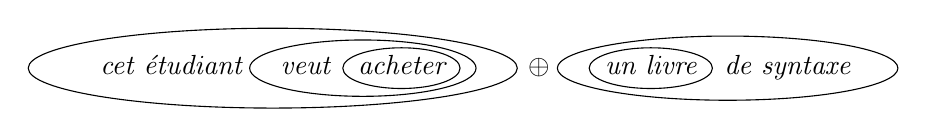
\begin{tikzpicture}
\matrix (matrix) [
                   matrix of nodes,
                   column sep=1em,
                   nodes={
                     font={\itshape\strut},
                     inner sep=0pt
                         }
                  ] 
  {
     cet étudiant  &[4pt] veut &  acheter   &[2em]   $\oplus$  &[1em] un livre &  de syntaxe\\
  };
\node [draw, ellipse, inner sep=-1pt, fit=(matrix-1-3)] {};
\node [draw, ellipse, inner xsep=-1pt, inner ysep=1pt, fit=(matrix-1-3) (matrix-1-2)] {};
\node [draw, ellipse, inner xsep=0pt, inner ysep=4pt, fit=(matrix-1-3) (matrix-1-2) (matrix-1-1)] {};

\node [draw, ellipse, inner sep=-1pt, fit=(matrix-1-5)] {};
\node [draw, ellipse, inner xsep=-1pt, inner ysep=2pt, fit=(matrix-1-5) (matrix-1-6)] {};
\end{tikzpicture}
\caption{\label{fig:}Combinaisons équivalentes}
\end{figure}

\Definition{\textstyleTermes{connexion}}
{Une \textstyleTermes{connexion} représente donc un \hi{ensemble de combinaisons équivalentes}. Il s’agit d’une «~abstraction~» de la notion de combinaison.}

D’aucun pourrait considérer qu’il aurait été beaucoup plus simple de définir la connexion comme une relation entre les mots et donc de ne regarder que les combinaisons de deux mots. C’est ce qui est habituellement fait dans les présentations de la syntaxe de dépendance. Deux raisons nous ont amené à procéder autrement. La première raison est que nous ne souhaitons pas présupposer que les connexions ont lieu entre les mots, parce que cela nous oblige à une définition préalable des mots, ce qui n’a rien de trivial, et que, par ailleurs, nous pensons que certaines connexions ne se réalisent pas entre les mots. La deuxième raison est que nous pensons que la connexion est fondamentalement une \hi{classe d’équivalence} \hi{de combinaisons} (voir définition dans l’\encadref{sec:3.2.15}) et que voir la connexion comme opérant seulement au niveau des mots est une vue parcellaire. On peut très bien envisager la connexion à d’autres niveaux de granularité, au niveau plus fin des syntaxèmes, comme à un niveau plus grossier (par exemple \textit{un livre} ${\oplus}$ \textit{de syntaxe}), voire comme les analyses en constituants immédiats, au niveau des constituants (voir \chapref{sec:3.4}). Un arbre de dépendance et un arbre de constituants peuvent très bien représenter exactement les mêmes connexions, mais ils le font avec des instances différentes : un arbre de dépendance représente les connexions par des combinaisons entre mots, tandis qu’un arbre de constituants représente les connexions par des combinaisons de constituants.


Notre définition permet d’appréhender plus clairement une question que l’on se pose généralement lorsqu’on aborde la syntaxe de dépendance : «~Les dépendances syntaxiques ont-elles réellement lieu entre les mots ?~». Nous pensons qu’on ne peut pas et qu’on ne doit pas répondre à cette question. Cette question n’a pas lieu d’être et c’est ce que montre notre définition de la connexion et celle de la dépendance qui en découle. Une connexion ne lie pas plus deux mots qu’elle ne lie toutes les unités plus larges qui incluent ces deux mots, tout comme elle peut lier des unités qui se trouvent en deçà du mot. Tout au plus peut-on se demander si les instances minimales des connexions lient des mots, mais la réponse à cette question varie selon les connexions et selon les critères définitionnels des unités syntaxiques choisis. Autrement dit, le fait que l’instance minimale d’une connexion lie deux mots n’est pas vraiment une propriété de la connexion en soi, mais bien davantage une conséquence des critères retenus pour définir les unités syntaxiques en général, lesquels critères sont ajustables et en partie indépendants des critères qui permettent de postuler une connexion donnée.


\maths[sec:3.2.15]{Définition formelle de la connexion}{%
    Nous avons défini ci-dessus une connexion comme un ensemble de combinaisons équivalentes. Cette définition peut être précisée. Commençons par donner une définition un peu plus formelle de l’équivalence entre deux combinaisons.

    Une combinaison A \textrm{${\oplus}$} B est \textstyleTermesapprof{plus fine} qu’une combinaison A’ \textrm{${\oplus}$} B’ si A est inclus dans A’ et B est inclus dans B’. Par exemple, la combinaison \textit{veut acheter} \textrm{${\oplus}$} \textit{un livre} est plus fine que la combinaison \textit{veut acheter} \textrm{${\oplus}$} \textit{un livre de syntaxe}.

    Deux combinaisons sont \textstyleTermesapprof{équivalentes} s’il existe une combinaison plus fine que les deux à la fois. Par exemple, \textit{acheter} \textrm{${\oplus}$} \textit{un livre de syntaxe} et \textit{cet étudiant veut acheter} \textrm{${\oplus}$} \textit{un livre} sont équivalentes car la combinaison \textit{acheter} \textrm{${\oplus}$} \textit{un livre} est plus fine que les deux.

    Dès qu’on a une \textstyleTermesapprof{relation d’équivalence} sur un ensemble, on peut considérer les objets à l’équivalence près. (Nous donnons une définition plus formelle d’une relation d’équivalence dans l’\encadref{sec:3.3.31} sur \textit{Dépendance, dominance et transitivité}.) Une relation d’équivalence \textstyleTermesapprof{partitionne} l’ensemble des objets en \textstyleTermesapprof{classes d’équivalence}. Donnons un exemple classique, celui des nombres rationnels. Les nombres rationnels sont les nombres qui peuvent s’écrire à l’aide d’une fraction comme \textsuperscript{3}/\textsubscript{4} ou \textsuperscript{257}/\textsubscript{23}. Les fractions \textsuperscript{3}/\textsubscript{4} ou \textsuperscript{75}/\textsubscript{100} sont deux fractions différentes qui représentent le même nombre rationnel. Elles sont donc équivalentes. Un nombre rationnel est une classe d’équivalence de fractions et il peut s’écrire d’une infinité de façons. De la même façon, les combinaisons sont les instances des connexions et une connexion peut être représentée par des combinaisons mettant en jeu des unités plus ou moins grandes.

    On peut maintenant définir la connexion à partir de la relation d’équivalence que nous venons de définir sur les combinaisons. De même qu’un nombre rationnel est une classe d’équivalence de fractions, une \textstyleTermesapprof{connexion} est une \hi{classe d’équivalence} \hi{de combinaisons}. Cette courte définition cache, on l’a compris, une opération d’abstraction complexe.
}
\section{Tests pour la connexion}\label{sec:3.2.16}

Les notions de connexion et d’unité syntaxique sont intimement liées. Dire qu’il y a une connexion entre les unités syntaxiques A et B revient à dire que AB ou BA forme une unité syntaxique. Les tests pour la connexion sont donc des tests pour vérifier qu’une portion d’un énoncé forme une unité syntaxique.

Nous avons donné trois tests pour décider si un segment de texte est une unité syntaxique :

\begin{itemize}
\item le test de commutation (\sectref{sec:3.2.10})
\item le test d’autonomisabilité illocutoire (\sectref{sec:3.2.11})
\item le test d’autonomisabilité prosodique (\sectref{sec:3.2.11})
\end{itemize}

Certains de ces tests sont suffisants (pour être une unité syntaxique) sans être pour autant nécessaires. C'est le cas des tests d'autonomisabilité
Nous verrons dans le \chapref{sec:3.4} d'autres tests suffisants pour caractériser une unité syntaxique, qui ne s’appliquent qu’à un sous-groupe d’unités syntaxiques, comme les constituants majeurs (\sectref{sec:3.4.10} \textit{Tests de constituance}).

Nous allons donner ici deux tests qui ne permettent pas de caractériser les unités syntaxiques, mais qui peuvent servir d'indices. Ces tests sont basés sur l'\hi{ordre linéaire} entre les unités syntaxiques, qu'on appelle généralement l'ordre des mots. Les principes généraux sont que l’ordre des unités syntaxiques dépend fortement des connexions : les unités syntaxiques qui sont connectées tendent à se \hi{placer} \hi{les unes par rapport aux autres} et \hi{les unes à côté des autres}. Ceci nous donne deux tests.

\Definition{test de déplacement}
{\textstyleTermes{test de déplacement}. Plus les placements des unités syntaxiques A et de B sont dépendants l’un de l’autre, plus il y a des chances que A et B soit connectés.}

\Definition{\textstyleTermes{test d’insertion}}
{\textstyleTermes{test d’insertion}. Si on ne peut pas insérer entre A et B d’unité qui ne soit pas connectée à A et B, alors A et B sont probablement connectés.}

Les énoncés des tests que nous avons donnés sont très généraux. Ils vont trouver des déclinaisons particulières selon les langues étudiées et les constructions concernées.

En français, l’usage le plus courant du test de déplacement concerne les dépendants du nom, qui, à l’exception de certains adjectifs, se placent tous à droite du nom dont ils dépendent. Nous allons donner deux illustrations. La première concerne les propositions :

\ea
  \ea \itshape Pierre a acheté une glace à la boulangerie.
  \ex \itshape Pierre a acheté une glace à la fraise.
  \z
\z

Dans les deux exemples, on a un groupe prépositionnel B introduit par \textit{à} dont on cherche à savoir s’il est connecté à A = \textit{une glace}. La permutation de A et B offre immédiatement une réponse :
\ea
    \ea[] {\itshape Pierre a acheté \textbf{à la boulangerie}  une glace.}\label{ex:boulangerie}
    \ex[*]{\itshape Pierre a acheté \textbf{à la fraise}  une glace.}\label{ex:fraise}
    \z
\z

La permutation est possible dans le premier cas, donc \textit{à la boulangerie} ne dépend pas de \textit{une glace}. Par contre, elle est impossible dans le deuxième cas, ce qui indique que \textit{à la fraise} dépend bien de \textit{une glace}. (Nous utilisons ici une autre propriété, spécifique au français, qui est que l’ordre des compléments à droite du verbe est relativement libre. Le même test serait plus difficile à appliquer dans une langue comme l’anglais où l’objet ne peut pas être facilement séparé du verbe.)

\begin{figure}
\begin{tikzpicture}
\node at (0,0) [ConcSet] (A) {Pierre a acheté};
\node [right=1em of A, ConcSet] (B) {une glace};
\node [right=1em of B, ConcSet] (C) {à la boulangerie};
\path (A.45) edge [bend left] (B)
      (A.60) edge [bend left] (C);
\end{tikzpicture}\medskip\\
\begin{tikzpicture}
\node at (0,0) [ConcSet] (A) {Pierre a acheté};
\node [right=1em of A, ConcSet] (B) {une glace};
\node [right=1em of B, ConcSet] (C) {à la fraise};
\path (A) edge [bend left] (B)
      (B) edge [bend left] (C);
\end{tikzpicture}
\caption{\label{fig:}Structures syntaxiques pour \REF{ex:boulangerie} et \REF{ex:fraise}}
\end{figure}

Le test de déplacement est particulièrement utile pour déterminer les dépendances au sein du groupe substantival (où les tests de pronominalisation ou de clivage ne peuvent pas être utilisés ; voir \chapref{sec:3.4} pour la présentation de ces tests). Considérons l’exemple suivant (extrait de l’article \textit{Seine} de la wikipédia) :

\ea \textit{La faible déclivité de la vallée de la Seine en Ile-de-France a causé la formation de multiples et profonds méandres.}
\label{ex:Seine}\z

On a ici trois segments prépositionnels, \textit{de la vallée}, \textit{de la Seine} et \textit{en Ile-de-France}, dont on doit déterminer le gouverneur. Le test de déplacement donne :

\ea
  \ea[*]{\textit{la faible déclivité \textbf{de la Seine}  de la vallée en Ile-de-France}}
  \ex[]{\textit{la faible déclivité \textbf{en Ile-de-France}  de la vallée de la Seine}}
  \z
\z
La non-déplaçabilité du segment \textit{de la Seine} indique qu’il est bien connecté au segment \textit{de la vallée}. À l’inverse la déplaçabilité de \textit{en Ile-de-France} indique qu’il n’en dépend pas. On a donc les connections suivantes :

\begin{figure}
\small\resizebox{\textwidth}{!}{%
\begin{tikzpicture}[every node/.style={inner sep=2pt}]
\node at (0,0) [ConcSet] (A) {la faible déclivité};                    
\node [right=1em of A, ConcSet] (B) {de la vallée};
\node [right=1em of B, ConcSet] (C) {de la Seine};
\node [right=1em of C, ConcSet] (D) {en Ile-de-France};

\path (A.45) edge [bend left] (B)
      (B)    edge [bend left] (C)
      (A.60) edge [bend left] (D);
\end{tikzpicture}}
\caption{\label{fig:}Rattachement des segments prépositionnels de \REF{ex:Seine}}
\end{figure}

Le test d’insertion peut être appliqué à notre premier exemple. Prenons un circonstanciel comme \textit{l’autre jour}, qui dépend du verbe, mais ne se connecte pas avec les unités A et B que nous considérons. On a :

\ea
  \ea[]{\textit{Pierre a acheté une glace \textbf{l’autre jour}  à la boulangerie.}}
  \ex[\textsuperscript{?}*]{\textit{Pierre a acheté une glace \textbf{l’autre jour} à la fraise.}}
  \z
\z
(Des énoncés tels que le deuxième sont tout à fait possibles avec une prosodie appropriée, où le segment \textit{à la fraise} est détaché. Mais ils ne pourraient être produits à l’écrit sans une ponctuation marquant le détachement.) Le fait que \textit{l’autre jour} peut être inséré entre A et B dans le premier cas et pas dans le deuxième indique que A et B sont connectés dans le premier cas et pas dans le deuxième.

De même, dans notre deuxième exemple, on peut vérifier que \textit{en Ile-de-France} ne peut pas être déplacé entre A = \textit{de la vallée} et B = \textit{de la Seine}, et donc que A et B son connectés :

\ea[*]{\textit{la faible déclivité de la vallée \textbf{en Ile-de-France} de la Seine}}\z
Le test d’insertion est un cas particulier de la propriété de projectivité que nous présentons dans la \sectref{sec:3.5.14} \textit{Projectivité et dépendance projective}. Cela revient à dire que certains liens de connexion ne peuvent pas se couper et que la configuration ci-dessous n’est pas possible.

\begin{figure}
\begin{tikzpicture}
\node at (0,0) [ConcSet] (A) {Pierre a acheté};
\node [right=1em of A, ConcSet] (B) {une glace};
\node [right=1em of B, ConcSet] (C) {l’autre jour};          
\node [right=1em of C, ConcSet] (D) {à la fraise};

\path (A) edge [bend left] (C)
      (B) edge [bend left] (D);
\end{tikzpicture}
\caption{\label{fig:}Configuration rejetée par le test d’insertion}
\end{figure}

Les deux tests que nous venons d’énoncer, le test de déplacement et le test d’insertion, sont des tests qui s’appliquent seulement à certaines connexions et qui dépendent de propriétés générales de la langue et de propriétés particulières de certaines constructions. Par exemple, si le test d’insertion s’applique bien à la connexion entre un nom et un complément de nom en français, il n’en sera pas de même dans des langues qui acceptent plus facilement des configurations non projectives ou pour d’autres constructions du français (voir la \encadref{sec:3.5.33} \textit{Non-projectivité} \textit{en français}).

\loupe[sec:3.2.17]{Connexion ternaire}{%
    Notre définition de la connexion présuppose que toute \hi{connexion} est \hi{binaire}, c’est-à-dire que les unités syntaxiques se combinent deux par deux. Ceci revient à supposer qu’on peut décomposer toute unité en deux morceaux. Nous n'avons pas vraiment d'exemples où une unité ne peut pas être décomposée en deux et nous n'introduirons donc pas, dans cet ouvrage, de \textstyleTermes{connexion ternaire}, c'est-à-dire de connexion liant trois éléments. Nous néanmoins aimerions souligner qu'il est possible de considérer des connexions ternaires et que cela a déjà été fait par différents auteurs.
    
    Les connexions ternaires sont introduites pour modéliser le fait qu'un élément grammatical marque la connexion entre deux éléments lexicaux. Par exemple, dans \textit{Ali parle à Zoé}, la préposition \textsc{à} marque la combinaison entre le verbe \textsc{parler} et le substantif \textsc{Zoé}. On peut donc adopter la représentation de la figure \ref{fig:ternaire}, où \textit{à} est placé sur le lien entre \textit{parle}  et \textit{Zoé}. Il s'agit bien d'une connexion ternaire liant directement \textit{parle}, \textit{à} et \textit{Zoé}.
    
    \begin{figure}[H]
		\begin{forest}for tree={font=\itshape}
			[parle
                [Ali]
                [Zoé, edge label={node[pos=0.25,right]{\textit{à}}}]
			]
		\end{forest}
    \caption{Arbre de dépendance avec une connexion ternaire\label{fig:ternaire}}
    \end{figure}

Le fait d'utiliser un lien ternaire ne permet pas d'indiquer si parmi la combinaison des trois éléments, il y a des combinaisons deux à deux possibles et, par exemple, si \textit{parle à} ou \textit{à Zoé} sont des combinaisons acceptables. L'objectif de ce type de représentation est généralement plus sémantique que syntaxique, en montrant qu'il y a une relation sémantique entre \textsc{parler} et \textsc{Zoé} qui est marquée syntaxiquement par la préposition sémantiquement vide \textsc{à}. 

Nous verrons, dans l'\encadref{sec:3.3.5} 
\textit{Historique des représentations syntaxiques par des diagrammes en dépendance},
un exemple de connexion ternaire pour la coordination proposé par Lucien Tesnière dans son article de \citeyear{tesniere1934comment}, où la conjonction de coordination \textit{et} est placée sur le lien entre deux conjoints. Cette analyse sera rediscutée dans l'\encadref{sec:3.4.26} \textit{Deux types d’arbres de constituants}, 
puis dans le \chapfuturef{19} sur les \textit{Listes} et le cas particulier de la coordination.
}
\section{Structures de connexion, granularité et critères}\label{sec:3.2.18}

Une \textstyleTermes{structure de connexion} est une représentation de la structure de l’énoncé contenant une instance de chaque connexion. Il existe plusieurs structures de connexion possibles selon la granularité de l’analyse et les critères pris en compte.

La \textstyleTermes{granularité} de l’analyse dépend de la \hi{taille des unités minimales} considérées. Pour une granularité donnée, la structure de connexion contient l’\textstyleTermes{instance minimale} de chaque connexion, c’est-à-dire l’instance reliant les plus petites unités considérées pour cette granularité. L’analyse syntaxique la plus fine prendra comme unités minimales les syntaxèmes. Il est courant que les analyses syntaxiques prennent comme unités minimales les mots. Une analyse au niveau de la structure discursive d’un texte peut prendre comme unités minimales les unités illocutoires (c’est-à-dire plus ou moins les phrases, voir partie 6). Une représentation syntaxique devra en tout cas contenir une instance de chaque connexion considérée.

La \hi{nature des critères} pris en compte amène également à considérer différentes structures de connexion. Prenons l’exemple suivant :

\ea \textit{Marie regardait Pierre}.\label{ex:regardait}\z

Cet énoncé contient, en plus des mots, les deux segments autonomisables \textit{Marie regardait} et \textit{regardait Pierre} et on a donc les combinaisons \textit{Marie} ${\oplus}$ \textit{regardait} et \textit{regardait} ${\oplus}$ \textit{Pierre}. Si l’on s’en tient aux unités syntaxiques autonomisables, on ne peut pas raffiner davantage ces connexions, mais on peut essayer en appliquant d’autres critères. La forme verbale \textit{regardait} peut être décomposée en \textit{regard-} ${\oplus}$ \textit{{}-ait} (c’est-à-dire un lexème et sa flexion). Les deux signes sont indissociables l’un de l’autre, donc on ne peut pas espérer former des unités autonomisables avec seulement l’un ou l’autre. En revanche, on peut voir que la commutation de \textit{{}-ait} avec d’autres flexions verbales n’a aucune incidence sur la possibilité de combiner la forme verbale avec l’objet \textit{Pierre}, alors que la commutation de \textit{regard-} avec d’autres lexèmes verbaux (\textit{parl-} ou \textit{rigol-}) rend cette combinaison impossible. On en déduit que c’est \textit{regard-} qui se combine avec \textit{Pierre}, car c’est lui qui contrôle la possibilité de se combiner ou pas avec \textit{Pierre}. Inversement, la commutation de \textit{regard-} avec d’autres lexèmes verbaux ne change rien à la combinaison avec le sujet \textit{Marie}, alors que la combinaison de \textit{{}-ait} avec d’autres flexions (l’infinitif ou l’impératif) bloque la combinaison avec le sujet. On en déduit que c’est \textit{{}-ait} qui se combine avec \textit{Marie}. Le critère que nous venons d’utiliser pour raffiner la connexion s’appelle le \hi{critère distributionnel sans effacement}, que nous présenterons à la \sectref{sec:3.3.13}.

Nous donnons dans les figures \ref{fig:regardait1} et \ref{fig:regardait2}
 deux instanciations des trois connexions entre les quatre unités considérées (\textit{Marie, regard-, -ait} et \textit{Pierre}). Dans la structure de la première figure, nous utilisons le seul critère d’autonomisabilité des unités pour déterminer les connexions. Dans la structure de la deuxième figure, nous ajoutons le critère de distributionnalité. Les deux analyses ont la même granularité, mais ne reposent pas sur les mêmes critères. La deuxième structure affine les connexions de la première structure en proposant des instances plus fines des connexions (voir l’\encadref{sec:3.2.15} sur la \textit{Définition formelle de la connexion} pour la relation de finesse entre combinaisons).

\begin{figure}
\begin{tikzpicture}
  \matrix [matrix of nodes, nodes={ConcSet},row sep=1em,column sep=1em] (matrix)
    {
      Marie & & & Pierre \\
       & regard- & -ait & \\     
    };
  \node [draw,ellipse,fit=(matrix-2-2) (matrix-2-3),inner sep=0pt] (row2) {};
  \draw (matrix-2-2) -- (matrix-2-3);
  \draw (matrix-1-1) -- (row2)
                     -- (matrix-1-4);
\end{tikzpicture}
\caption{Structure de connexion avec critère d’autonomisabilité pour \REF{ex:regardait}}
\label{fig:regardait1}
\end{figure}

\begin{figure}
\begin{tikzpicture}
  \matrix [matrix of nodes, nodes={ConcSet},row sep=1em,column sep=1em] (matrix)
    {
      & -ait & & Pierre\\
      Marie & & regard- & \\
    };
  \draw (matrix-2-1) -- (matrix-1-2)
                     -- (matrix-2-3)
                     -- (matrix-1-4);
\end{tikzpicture}
\caption{Structure de connexion avec critère distributionnelpour \REF{ex:regardait}}
\label{fig:regardait2}
\end{figure}

Dans la suite de ce chapitre, nous travaillerons avec les unités syntaxiques autonomisables et donc avec le grain des mots, qui sont les plus petites unités syntaxiques faiblement autonomisables (voir \chapfuturef{14}).

\section{Structure de connexion et unités}\label{sec:3.2.19}

Nous avons vu deux façons de définir une structure de connexion dans la section précédente. Dans la première, nous nous sommes entièrement basés sur les unités que l’on pouvait considérer dans la phrase \textit{Marie regardait Pierre}, à savoir : \textit{Marie, Pierre, regar-, -ait, regardait, Marie regardait, regardait Pierre} et la phrase entière. Dès qu’une unité est la combinaison de deux sous-unités, nous postulons une combinaison : \textit{regardait} = \textit{regard-} ${\oplus}$ \textit{{}-ait}, \textit{Marie regardait} = \textit{Marie} ${\oplus}$ \textit{regardait} et \textit{regardait Pierre} = \textit{regardait} ${\oplus}$ \textit{Pierre}, mais aussi \textit{Marie regardait Pierre} = \textit{Marie} ${\oplus}$ \textit{regardait Pierre} et \textit{Marie regardait Pierre} = \textit{Marie regardait} ${\oplus}$ \textit{Pierre}. Certaines combinaisons sont équivalentes et correspondent à la même connexion : \textit{Marie} ${\oplus}$ \textit{regardait} et \textit{Marie} ${\oplus}$ \textit{regardait Pierre} d’une part, et \textit{regardait} ${\oplus}$ \textit{Pierre} et \textit{Marie regardait} ${\oplus}$ \textit{Pierre} d’autre part. Pour construire la structure de connexion, nous prenons l’instance minimale de chaque connexion, ce qui nous donne la structure de gauche de la section précédente. Nous avons pu construire cette structure de connexion à partir de l’ensemble des unités et de lui seul. Inversement, la structure de connexion nous permet de retrouver l’ensemble des unités. Pour cela, il faut imaginer qu’on a des ciseaux et qu’on peut couper des connexions pour ne garder que des bouts de la structure. Chaque bout obtenu est une unité. Par exemple, on peut couper le lien entre \textit{Marie} et \textit{regardait} et il nous reste \textit{regardait Pierre}. On peut tout couper et obtenir les unités minimales, y compris \textit{regard-} et \-\textit{{}-ait}. En revanche, on ne peut obtenir de combinaison de \textit{Marie} avec seulement \textit{regard-} ou \-\textit{{}-ait}, car \textit{Marie} est connecté à tout \textit{regardait}. Dans le cas où la structure de connexion est définie en se basant uniquement sur des critères définissant les unités syntaxiques, nous avons une \hi{dualité} parfaite entre la structure de connexion et l’ensemble des unités. (La notion de \textit{dualité} est présentée dans l’\encadref{sec:2.2.8} éponyme.)

Dans la figure de droite de la section précédente, nous avons utilisé un critère supplémentaire, le critère distributionnel, pour affiner la structure et postuler les combinaisons \textit{Marie} ${\oplus}$ \textit{-ait} et \textit{regard-} ${\oplus}$ \textit{Pierre}. Ces combinaisons ne sont plus basées sur des unités : nous ne considérons pas que \textit{Marie} ${\oplus}$ \textit{-ait} ou \textit{regard-} ${\oplus}$ \textit{Pierre} forment des unités. Il n’y a plus de dualité entre la structure de connexion et l’ensemble des unités syntaxiques considérées.


\loupe[sec:3.2.20]{Les limites de la dualité}{%
    Timothy \citet{osborne2019dependency} propose d’appeler \textstyleTermesapprof{catena} (‘chaîne’ en latin) toute portion connexe d’un arbre de dépendance. (Le terme est un peu trompeur, puisque les catenae peuvent brancher et ne pas être stricto sensu des chaînes.) Les catenae sont toutes les unités obtenues lorsqu’on découpe l’arbre de dépendance en morceaux en coupant des dépendances. Les catenae comprennent la quasi-totalité des unités qui jouent un rôle dans la langue : non seulement tous les constituants considérés par les grammaires de constituants, y compris les projections intermédiaires (voir la \sectref{sec:3.4.14} \textit{Arbre de constituants binaire}), mais aussi les formes verbales complexes (\textit{a mangé}), les collocations (\textit{avoir besoin}), les locutions (\textit{sur le point} (\textit{de} Vinf)) ou encore les nucléus verbaux dont nous montrerons le rôle dans l’extraction (\textit{le livre que tu} \textbf{\textit{veux}} \textbf{\textit{que}} \textit{je} \textbf{\textit{lise}}) et d’autres phénomènes au \chapfuturef{19}. Osborne tire argument du fait que ces unités peuvent ainsi être facilement déduites d’un arbre de dépendance pour justifier le fait qu’un arbre de dépendance encode la structure syntaxique de manière plus satisfaisante qu’un arbre de constituants (voir la \sectref{sec:3.2.25} sur l’\textit{Analyse en constituants immédiats}).

    Nous pensons néanmoins qu’il y a un problème méthodologique à vouloir partir d’un arbre de dépendance pour en déduire les unités de la langue. D’une part, la définition d’un arbre de dépendance est basée sur une structure de connexion qui est une façon de représenter de manière structurée et condensée l’ensemble des unités syntaxiques et il semble difficile de définir cette structure sans avoir défini au préalable ce qu’est une unité syntaxique ; ce n’est donc pas les unités qui se déduisent de l’arbre de dépendance, c’est l’arbre de dépendance qui se déduit de l’ensemble des unités considérées.~D’autre part, la définition d’un arbre de dépendance est \hi{plus complexe} que l’identification des unités syntaxiques et fait appel à de nombreux critères (les critères utilisés pour l’identification des unités syntaxiques, mais aussi le critère distributionnel, déjà évoqué à la \sectref{sec:3.2.18}, et d’autres encore que nous introduirons au \chapref{sec:3.3}). Ces critères permettent en particulier de mettre en évidence une hiérarchie qui n’est pas nécessaire pour définir les unités syntaxiques. Par ailleurs, en raison de la prise en compte de critères supplémentaires, les catenae, c’est-à-dire les portions connexes de l’arbre de dépendance, ne sont pas toutes des unités syntaxiques et il n’y a donc plus de dualité parfaite entre l’ensemble des unités syntaxique et la structure de dépendance. Certaines des propriétés utilisées pour définir l’arbre de dépendance (comme le critère distributionnel) ne sont pas aisément transférables en des propriétés des unités et certaines des catenae de l’arbre de dépendance n’ont pas d’intérêt théorique a priori. Par exemple, pour une phrase comme \textit{Le chien dort}, il faudra connecter \textit{dort} à \textit{chien} ou à \textit{le} pour obtenir un arbre de dépendance, mais ni \textit{le dort} ni \textit{chien dort} n’est une unité intéressante. (Voir le \chapref{sec:3.3} pour une discussion approfondie des critères qui permettent de construire un arbre de dépendance.)
}
\section{Arbre de fragmentation}\label{sec:3.2.21}

Il n’est pas nécessaire d’identifier toutes les unités syntaxiques pour obtenir la structure de connexion. Une des façons d’obtenir les unités syntaxiques et la structure de connexion qui lui correspond est de procéder par décompositions successives d’un énoncé. On commence par chercher des décompositions possibles de l’énoncé en deux unités syntaxiques, puis l’on choisit une des décompositions. Pour chacune des deux unités obtenues, on recommence : on cherche des décompositions possibles en deux unités et on en choisit une. Et ainsi de suite, jusqu’à arriver aux unités minimales (par exemple les mots ou les syntaxèmes). Une série successive de décompositions est appelée une \textstyleTermes{fragmentation} de l’énoncé et l’ensemble des unités obtenues dans une fragmentation donnée en sont les \textstyleTermes{fragments}.

Donnons des exemples de fragmentations de l’énoncé \REF{ex:livredesyntaxe} \textit{Cet étudiant veut acheter un livre de syntaxe}. Nous limitons nos fragmentations aux unités autonomisables.

\ea
\ea ((\textit{cet} ${\oplus}$ \textit{étudiant}) ${\oplus}$ (\textit{veut} ${\oplus}$ \textit{acheter})) ${\oplus}$ ((\textit{un} ${\oplus}$ \textit{livre}) ${\oplus}$ (\textit{de} ${\oplus}$ \textit{syntaxe}))\label{ex:fragmentation:1}
\ex (\textit{cet} ${\oplus}$ \textit{étudiant}) ${\oplus}$ (\textit{veut} ${\oplus}$ (\textit{acheter} ${\oplus}$ (\textit{un} ${\oplus}$  (\textit{livre} ${\oplus}$ (\textit{de} ${\oplus}$ \textit{syntaxe})))))
\ex ((\textit{cet} ${\oplus}$ \textit{étudiant}) ${\oplus}$  \textit{veut}) ${\oplus}$ ((\textit{acheter} ${\oplus}$ (\textit{un} ${\oplus}$ \textit{livre})) ${\oplus}$ (\textit{de} ${\oplus}$ \textit{syntaxe}))
\z
\z

On peut représenter une fragmentation par une structure arborescente, appelée un \textstyleTermes{arbre de fragmentation} : chaque nœud de l’arbre représente un fragment, les feuilles de l’arbre étant les fragments minimaux considérés (les mots dans notre exemple). Les branches de l’arbre représente la relation entre un fragment et un des deux sous-fragments obtenu lors de la décomposition. Nous donnons l’arbre de fragmentation de la première de nos trois fragmentations.

\begin{figure}
\begin{tikzpicture}[every node/.style={font=\strut\itshape}]
\begin{scope}[
              every node/.style={CircleNode},level distance=2\baselineskip,
              level 1/.style={sibling distance=60mm},
              level 2/.style={sibling distance=30mm},
              level 3/.style={sibling distance=15mm}
             ]
      \node (root) {}
        child { node{} 
                child { node{} 
                    child { node{} }
                    child { node{} }
                      }
                child { node{} 
                    child { node{} }
                    child { node{} }
                      } 
               }
        child { node{} 
                child { node{} 
                    child { node{} }
                    child { node{} }
                      }
                child { node{} 
                    child { node{} }
                    child { node{} }
                      } 
               };
    \end{scope}
    \node[below=1pt of root-1-1-1] {cet};
    \node[below=1pt of root-1-1-2] {étudiant};
    \node[below=1pt of root-1-2-1] {veut};
    \node[below=1pt of root-1-2-2] {acheter};
    \node[below=1pt of root-2-1-1] {un};
    \node[below=1pt of root-2-1-2] {livre};
    \node[below=1pt of root-2-2-1] {de};
    \node[below=1pt of root-2-2-2] {syntaxe};
\end{tikzpicture}
\caption{\label{fig:}L’arbre pour la fragmentation \REF{ex:fragmentation:1}}
\end{figure}

\section{De la fragmentation à la connexion}\label{sec:3.2.22}

On peut définir la structure de connexion d’un énoncé à partir de toutes les fragmentations possibles de cet énoncé. Il suffit de prendre toutes les combinaisons obtenues, puis de sélectionner parmi les ensembles de combinaisons équivalentes l’instance minimale (voir la \sectref{sec:3.2.18} \textit{Structures de connexion, granularité et critères}). Si cette méthode est la plus efficace du point de vue théorique, ce n’est pas celle que l’on utilise en pratique. Il est inutile de considérer toutes les fragmentations, toutes les unités et toutes les combinaisons qu’induit un énoncé que l’on souhaite analyser. Il suffit en fait de calculer \hi{n’importe} \hi{quelle fragmentation} de l’énoncé, puis d’obtenir la structure de connexion par des raffinements successifs des combinaisons de cette fragmentation. Il suffit, pour chaque combinaison A ${\oplus}$ B et pour une décomposition de A en X ${\oplus}$ Y, de regarder si l’une des combinaisons X ${\oplus}$ B ou Y ${\oplus}$ B peut raffiner la combinaison A ${\oplus}$ B. On va ainsi raffiner chaque connexion jusqu’à obtenir une combinaison minimale qui ne peut plus être raffinée.

Prenons l’exemple de la section précédente et l’arbre de fragmentation que nous avons dessiné. On veut raffiner la combinaison A ${\oplus}$ B avec A = \textit{cet étudiant} et B = \textit{veut acheter}. A se décompose en X ${\oplus}$ Y avec X = \textit{cet} et Y = \textit{étudiant}. Aucune des deux combinaisons \textit{cet veut acheter} et \textit{étudiant veut acheter} ne forme une unité syntaxique et on ne peut donc raffiner ainsi. À l’inverse, B se décompose en \textit{veut} ${\oplus}$ \textit{acheter} et \textit{cet étudiant veut} est une unité syntaxique. On peut donc raffiner la combinaison A ${\oplus}$ B en A ${\oplus}$ \textit{veut}. En continuant ainsi, on obtient la structure de connexion de la figure \ref{fig:livredesyntaxe}.

\begin{figure}
\begin{tikzpicture}
  \matrix [matrix of nodes, 
           nodes={ConcSet,font=\footnotesize\itshape}, 
           row sep=1em, 
           column sep=.333em] (matrix)
          {
            cet & étudiant & & acheter & & & de & syntaxe\\
                &          & veut & & un & livre & & \\ 
          };
  \node [draw,ellipse,inner sep=0pt,fit = (matrix-1-1) (matrix-1-2)] (row11) {};
  \node [draw,ellipse,inner sep=0pt,fit = (matrix-2-5) (matrix-2-6)] (row21) {};
  \node [draw,ellipse,inner sep=0pt,fit = (matrix-1-7) (matrix-1-8)] (row12) {};
  \draw (matrix-1-1) -- (matrix-1-2)
        (matrix-2-5) -- (matrix-2-6)
        (matrix-1-7) -- (matrix-1-8);
  \draw (row11) -- (matrix-2-3) 
                -- (matrix-1-4)
                -- (row21)
                -- (row12);
\end{tikzpicture}
\caption{\label{fig:livredesyntaxe}Structure de connexion pour \REF{ex:livredesyntaxe}}
\end{figure}

\maths[sec:3.2.23]{Graphe à bulles et polygraphe}{%
Pour représenter la structure de connexion, nous avons utilisé une structure que nous proposons d’appeler un \textstyleTermesapprof{graphe à bulles}. Rappelons qu’un \hi{graphe} est un ensemble d’éléments, appelés \hi{nœuds}, reliés deux à deux par des liens, appelés \hi{arêtes} (voir l’\encadref{sec:1.2.3} sur \textit{Graphe et arbre}). Dans un graphe à bulles, les \hi{sommets} d’une arête peuvent être des \hi{bulles} contenant plusieurs nœuds. Une arête qui relie des nœuds simples est dite \textstyleTermesapprof{élémentaire} et une arête dont un des sommets au moins est une bulle est \textstyleTermesapprof{non élémentaire}.

Les structures de connexion ne sont pas n’importe quel graphe à bulles. D’une part, les bulles ne se chevauchent pas, c’est-dire que deux bulles sont ou bien disjointes ou bien incluses l’une dans l’autre. D’autre part, la structure a une propriété de \hi{connexité} (voir également l’\encadref{sec:1.2.3}) : la structure est formée de grandes bulles qui forment un réseau connexe et l’intérieur de chaque bulle est lui-même un réseau connexe de bulles et ceci jusqu’aux bulles élémentaires que sont les nœuds.

Enfin, les structures de connexion ont généralement la propriété de binarité suivante : chaque bulle se décompose en deux bulles connectées entre elles. Il est alors possible d’utiliser un autre mode de représentation, où les bulles ne sont pas représentées : un lien dont le sommet est une bulle composée de deux sous-bulles connectées entre elles sera attribué au lien entre les deux sous-bulles. On obtient une nouvelle structure, que nous appelons un \textstyleTermesapprof{polygraphe}, où une arête peut avoir pour sommet un nœud ou une arête. Nous donnons ci-dessous une version polygraphique de la structure connexion de la section précédente.

\begin{figure}[H]
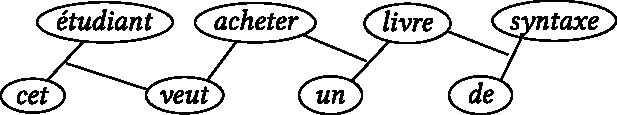
\includegraphics[scale=.75]{figures/ceetudiantveutacheterunlivredesyntaxe.pdf}
% % % \begin{tikzpicture}
% % %   \matrix [matrix of nodes,
% % %            nodes={ConcSet,font=\footnotesize},
% % %            row sep=1em,
% % %            column sep=.333em,
% % %            ampersand replacement=\&] (matrix)
% % %     {
% % %       \& étudiant \& \& acheter \& \& livre \& \& syntaxe\\
% % %       cet \& \& veut \& \& un \& \& de \& \\
% % %     };
% % %     \coordinate (intersection1) at ($ (matrix-1-2) !.5! (matrix-2-1) $);
% % %     \coordinate (intersection2) at ($ (matrix-1-6) !.5! (matrix-2-5) $);
% % %     \coordinate (intersection3) at ($ (matrix-1-8) !.5! (matrix-2-7) $);
% % %     \draw (intersection1) -- (matrix-2-1);
% % %     \draw (intersection1) -- (matrix-1-2);
% % %     \draw (intersection1) -- (matrix-2-3);
% % %     \draw (matrix-2-3)    -- (matrix-1-4);
% % %     \draw (intersection2) -- (matrix-1-4);
% % %     \draw (intersection2) -- (matrix-2-5);
% % %     \draw (intersection2) -- (matrix-1-6);
% % %     \draw (intersection3) -- (matrix-1-6);
% % %     \draw (intersection3) -- (matrix-2-7);
% % %     \draw (intersection3) -- (matrix-1-8);
% % % \end{tikzpicture}         
\caption{\label{fig:}Polygraphe représentant une structure de connexion}
\end{figure}
}


\loupe[sec:3.2.24]{Cycle de connexions}{%
    Il peut arriver qu’une unité ABC possède comme sous-unités à la fois AB, BC et AC et que les trois combinaisons A \textrm{${\oplus}$} B, B \textrm{${\oplus}$} C et A \textrm{${\oplus}$} C soient possibles, ce qui donne un \hi{cycle} (non orienté) de connexions. (On verra, lorsqu’on considérera la dépendance et que les connexions sont orientées, qu’il ne peut pas s’agir d’un cycle orienté ; voir la \sectref{sec:3.3.4} \textit{Structure de dépendance et arbre de dépendance}.) Cette situation se rencontre avec les exemples suivants de la figure \ref{fig:cycles}.

\begin{figure}[H]
\caption{\label{fig:cycles}Structures de connexion avec cycle}
\begin{subfigure}[c]{.5\linewidth}
\centering
\caption{\textit{Marie commet une faute envers Pierre.}}
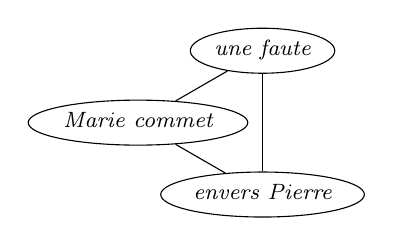
\begin{tikzpicture}
  \graph [clockwise=3,radius=3em, phase=180, nodes={draw,ellipse,inner sep=1pt,font=\footnotesize\itshape\strut}] {
     {[cycle] {Marie commet}, {une faute}, {envers Pierre}  }
  };
\end{tikzpicture}
\end{subfigure}%
\begin{subfigure}[c]{.5\linewidth}
\centering
\caption{\textit{Je l’ai vu hier à l’école.}}
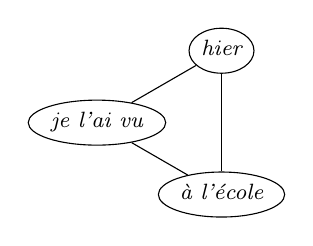
\begin{tikzpicture}
  \graph [clockwise=3,radius=3em, phase=180, clockwise=3,nodes={draw,ellipse,inner sep=1pt,font=\footnotesize\itshape\strut}] {
     {[cycle] {je l’ai vu}, {hier}, {à l’école} }
  };
\end{tikzpicture}
\end{subfigure}\medskip\\
\begin{subfigure}[c]{.5\linewidth}
\centering
\caption{\textit{la montée du nationalisme en Catalogne}}
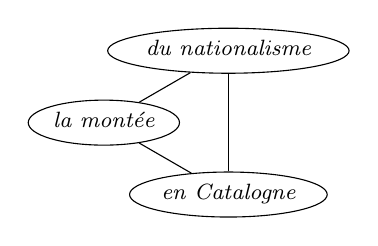
\begin{tikzpicture}
  \graph [clockwise=3,radius=3em, phase=180, clockwise=3,nodes={draw,ellipse,inner sep=1pt,font=\footnotesize\itshape\strut}] {
     {[cycle] {la montée}, {du nationalisme}, {en Catalogne} }
  };
\end{tikzpicture}
\end{subfigure}%
\end{figure}

Dans la phrase a, on peut à la fois considérer comme acceptables les unités syntaxiques \textit{commet une faute, commet envers Pierre} et \textit{une faute envers Pierre}. Il s’ensuit que le rattachement du complément \textit{envers Pierre} à \textit{une faute} plutôt qu’à \textit{commet} est incertain, que l’un ou l’autre ne change pas le sens.

La deuxième b pose les mêmes problèmes. Il est assez clair que \textit{hier} et \textit{à l’école} sont tous deux des compléments connectés à la construction verbale (\textit{je l’ai vu hier, je l’ai vu à l’école}), mais par ailleurs \textit{hier à l’école} semble aussi fonctionner aussi comme unité syntaxique (\textit{C’est hier à l’école que je l’ai vu} ; \textit{Tu l’as vu} ? \textit{Oui, hier à l’école}.)

L'exemple c est du même type encore. S’agit-il du \textit{nationalisme en Catalogne} dont on évoque la montée ou bien du nationalisme dont on considère \textit{la montée en Catalogne}. Peu importe, le sens est à peu près le même et le locuteur n’a pas vraiment les moyens de choisir une connexion plutôt que l’autre. Comme bien sûr \textit{la montée} et \textit{du nationalisme} sont connectés, on a, à nouveau, un cycle potentiel.

Le fait que les trois connexions sont possibles ne signifie pas que les trois connexions coexistent dans la production ou l’analyse de ces exemples. Il est probable que la prosodie produite par le locuteur privilégie une décomposition plutôt qu’une autre et donc une connexion plutôt qu’une autre. On peut penser que, une fois que le destinataire d’un tel énoncé a récupéré une structure connexe satisfaisante, il ne cherche pas à voir s’il pourrait encore la compléter pour obtenir des cycles. En conclusion, nous pensons que la structure syntaxique d’un énoncé peut être potentiellement cyclique, que la manipulation de structures cycliques ne pose pas de problèmes théoriques ou pratiques particuliers, mais nous ne pouvons pas savoir si les locuteurs manipulent ou non des structures syntaxiques cycliques lorsqu’ils produisent ou analysent un énoncé.
}
\section{Analyse en constituants immédiats}\label{sec:3.2.25}

La fragmentation d’un énoncé est à la base de l’\textstyleTermes{analyse en constituants immédiats} (\textstyleTermes{ACI}) initiée par Leonard \citet{bloomfield1933language} et popularisée à la fin des années 1950 par la formalisation qu’en a donnée Noam \citet{chomsky1957syntactic} (voir l’\encadref{sec:3.5.29} sur les \textit{Grammaires de réécriture}). L’ACI fait une hypothèse supplémentaire par rapport à l’approche que nous développons : elle suppose qu’\hi{une seule fragmentation} d’un énoncé est \hi{légitime} et que cette unique fragmentation définit les constituants de l’énoncé. L’arbre de fragmentation correspondant est appelé un \textstyleTermes{arbre de constituants}. (Cet arbre est aussi souvent appelé \textit{arbre syntagmatique}, mais nous ne retiendrons pas ce terme qui ne correspond pas à l’usage que nous faisons, à la suite de Saussure, du terme \textit{syntagme}. Voir l’\encadref{sec:3.1.5} \textit{À chacun son syntagme}.)

Henry \citet{gleason1955introduction}, qui est l’un des auteurs qui a défini l’arbre de constituant avec le maximum de rigueur, est explicite sur la nécessité de choisir une fragmentation parmi toutes celles possibles. Le début de sa définition est tout à fait compatible avec la notre : «~Nous pouvons, comme première hypothèse, considérer que chacun des [mots de l’énoncé considéré] a une relation énonçable avec chaque autre mot. Si l’on peut décrire ces interrelations complètement, on aura décrit la syntaxe de l’énoncé dans son entièreté. […] On pourrait commencer par marquer ces paires de mots qui sont ressenties comme ayant les relations les plus étroites.~» Puis sans justification aucune, il ajoute : «~Nous allons aussi imposer la règle que chaque mot peut être marqué comme appartenant à seulement une telle paire.~» Il poursuit en déclarant que la méthode pour trouver la meilleure paire parmi toutes celles possibles est «~le problème de base de la syntaxe~» («~the basic problem of syntax~»), tout en admettant que sa méthode est un peu désordonnée et ne fonctionne pas complètement.

Nous ne partageons pas le point de vue de Gleason et ses contemporains. Nous avons sciemment donné une définition peu restrictive de la notion d’\textit{unité syntaxique}. La plupart des linguistes de la seconde moitié du 20\textsuperscript{e} siècle, et notamment les courants théoriques dit générativistes, issus de l’école chomskyenne, ont défendu que seules les unités qu’ils appellent les \textstyleTermes{constituants syntaxiques} sont des unités syntaxiques légitimes. Nous pensons pour notre part que les constituants syntaxiques sont des unités syntaxiques particulières, certes remarquables, mais qu’il n’y a pas lieu de ne pas considérer les autres unités syntaxiques.

Obtenir une seule décomposition suppose d’avoir des critères beaucoup plus restrictifs que les nôtres pour la définition des unités syntaxiques. Si l’on se place dans ce cadre, on ne peut plus proposer de décomposer \textit{un livre de syntaxe}~à la fois en \textit{un} ${\oplus}$ \textit{livre de syntaxe} et en \textit{un livre} ${\oplus}$ \textit{de syntaxe}. \textbf{Il faut choisir entre les deux décompositions.} Une telle approche suppose par exemple que l’énoncé \textit{Cet étudiant veut acheter un livre de syntaxe} peut être décomposé en \textit{cet étudiant} ${\oplus}$ \textit{veut acheter un livre de syntaxe} à l’exclusion de toute autre décomposition. Il faut donc proposer des critères qui fassent de ces deux fragments les deux seuls fragments acceptables (du point de vue de ces critères). Nous pensons que c’est difficile et, qui plus est, inutile. (Nous discuterons cette question en long et en large au \chapref{sec:3.4}.) Au contraire, en considérant toutes les fragmentations possibles d’un énoncé, on obtient une structure plus riche et finalement plus simple.

Les constituants sont des unités syntaxiques particulières, plus difficiles à caractériser que les unités syntaxiques en général. Il faut pour caractériser les constituants des critères additionnels et notamment faire intervenir la notion de tête dont il sera question au \chapref{sec:3.3}. Dans le \chapref{sec:3.4}, nous verrons qu’il est possible de caractériser, parmi toutes les fragmentations possibles, différentes fragmentations correspondant à un arbre de constituants et que ces fragmentations, accompagnée de l’indication des têtes, permettent de récupérer directement la structure de connexion et donc les autres fragmentations. Nous présenterons en particulier dans l’\encadref{sec:3.4.18} la \textit{Syntaxe X-barre} qui est la version la plus aboutie de l’ACI.

\loupe[sec:3.2.26]{Traitement cognitif des connexions}{%
    Bien que cela soit en dehors de notre champ de compétence, nous nous risquons à faire des hypothèses sur le traitement cognitif des connexions. Nous venons de dire que nous pensions que les locuteurs construisent des connexions. La question qui se pose est entre quoi les locuteurs créent-ils des connexions ? Ou dit autrement : quelle instance des connexions les locuteurs construisent-ils ?

    La syntaxe de dépendance traditionnelle répond, à la suite de Tesnière, que les connexions se font entre mots (voir la citation de Tesnière à la \sectref{sec:3.2.8}). La syntaxe générative, si on suit l’analyse en constituants immédiats, répond que les locuteurs connectent les syntaxèmes pour former des constituants de plus en plus gros et que la phrase entière est obtenue par la combinaison de deux constituants que sont le sujet et le groupe verbal. Il est clair pour nous que la syntaxe de dépendance est beaucoup plus proche de la réalité cognitive. On peut néanmoins raisonnablement se demander si toutes les connexions se font entre mots. Existe-t-il des connexions qui s’instancient entre syntaxèmes de mots différents ? Existe-t-il des connexions qui s’instancient entre unités plus larges que le mot ?

    Il est généralement admis que les locuteurs traitent les énoncés de manière \textstyleTermesapprof{incrémentale}, c’est-à-dire au fur et à mesure qu’ils les perçoivent. Une expérience classique est celle des \textstyleTermesapprof{garden paths} (en anglais \textit{to lead somebody up the garden path} signifie ‘mener quelqu’un en bateau’). Lisez les deux phrases suivantes :

    \ea
      \ea \itshape L’espion reconduit à la frontière un diplomate américain.
      \ex \itshape L’espion reconduit à la frontière est un diplomate russe.
      \z
    \z

    Lorsqu’on suit le mouvement des yeux d’un lecteur (on appelle cette méthode l’\textit{eye-tracking}), on observe une saccade régressive sur la deuxième phrase, c’est-à-dire que lorsque le lecteur tombe sur la deuxième forme verbale, \textit{est}, il revient sur la première, \textit{reconduit}, puis revient sur \textit{est}. Ceci tend à prouver que l’analyse est globalement incrémentale, que les mots sont analysés et connectés au fur et à mesure de la lecture, mais que toute analyse qui est infirmée par la suite nécessite un \textstyleTermesapprof{retour en arrière} (angl. \textit{backtracking}) pour détricoter l’analyse en cours.

    Le fait que l’analyse soit globalement incrémentale n’induit pas nécessairement que les syntaxèmes sont systématiquement traités les uns après les autres. Il est probable que les locuteurs traitent le texte par \hi{petits blocs successifs} et que ces blocs contiennent quelques mots. Donc, d’une part, le locuteur va connecter ces blocs entre eux (voir notamment la stratégie d’analyse de la \encadref{sec:3.5.16} sur le \textit{Flux de dépendances}) et d’autre part, il va les décomposer en syntaxèmes et éventuellement raffiner les connexions.

    La \hi{prosodie} joue certainement un grand rôle : elle permet, nous pensons, de segmenter une production et d’indiquer pour chacun des segments obtenus qu’il peut être traité indépendamment de la suite et recevoir une structure connexe. La prosodie sert donc (en plus de ses autres fonctions liées à l’expressivité ou au marquage de l’illocution) à guider le traitement de la chaîne parlée par l’interlocuteur.

    Prenons un exemple : \textit{L’autre jour, j’ai rencontré quelqu’un que j’avais pas revu depuis l’école primaire}. Même si \textit{l’autre jour} est détaché et que le reste de l’énoncé forme une unité plus cohésive (un noyau, nous verrons), on n’attend pas d’avoir la totalité du noyau pour connecter \textit{l’autre jour} à la construction verbale. Le complément d’objet direct de \textsc{rencontrer} est un groupe substantival assez long : \textit{quelqu’un que j’avais pas revu depuis l’école primaire}. Même s’il faut avoir traité l’ensemble de ce groupe pour savoir ‘ce que j’ai rencontré’, on n’a pas besoin d’attendre d’avoir traité la relative pour connecter \textit{quelqu’un} à \textit{j’ai rencontré}. Il est d’ailleurs assez probable que l’énoncé soit segmenté prosodiquement de la façon suivante : \textit{l’autre jour {\textbar} j’ai rencontré quelqu’un {\textbar} que j’avais pas revu {\textbar} depuis l’école primaire}, puisque les groupes accentuels tendent à faire autour de 6 syllabes, et qu’il faut que, à chaque frontière de groupe accentuel (marquées ici par {\textbar} ), l’ensemble de ce qui précède reçoive une analyse syntaxique complète. Chacun des quatre groupes prosodiques peut recevoir une analyse complète indépendamment des autres groupes, puis être connecté aux autres, ce qui donne la structure de la figure \ref{fig:rencontre}/

    \begin{figure}[H]
    \begin{tikzpicture}
    \node at (0,0)  [ConcSet,font=\small] (A) {\textit{l’autre jour}};
    \node at (2.5,-1) [ConcSet,font=\small] (B) {\textit{j’ai rencontré quelqu’un}};
    \node at (5,-2) [ConcSet,font=\small] (C) {\textit{que j’avais pas revu}};
    \node at (7.5,-3) [ConcSet,font=\small] (D) {\textit{depuis l’école primaire}};
    \path [draw] (A.north east) edge [out=45, in=80] (B)
                 (B.north east) edge [out=45, in=90] (C.45)
                 (C.north east) edge [out=45, in=90] (D.45);
    \end{tikzpicture}
    \caption{Structure de connexion induite par la prosodie}
    \label{fig:rencontre}
    \end{figure}

    Nous pouvons dire pour conclure que la représentation de l’organisation syntaxique d’un énoncé par une structure de connexions présente des avantages pour qui voudrait étudier plus avant le traitement cognitif de la parole et de la lecture, permettant de rendre compte d’une connexion à différents niveaux de granularité, d’attribuer des analyses à n’importe quelle portion d’un énoncé et de construire la structure d’un énoncé de manière incrémentale.
}
\exercices{%\label{sec:3.2.27}
    \exercice{1} 
    \begin{enumerate}[label=\alph*.]
    \item Expliquez quelles contraintes agissent sur la réalisation du sens ‘rapide’ dans les deux phrases suivantes :
      \begin{enumerate}[label=(\arabic*)]
      \item   \textit{{Zoé a jeté un coup d’œil} \textbf{{rapide}}  {dans la pièce.}}
      \item   \textit{{Zoé a regardé} \textbf{{rapidement}}  {dans la pièce}.}
      \end{enumerate}
    \item Quelles contraintes agissent sur la réalisation de ‘épée’ dans les deux phrases suivantes ?
     \begin{enumerate}[label=(\arabic*),resume]
      \item \textit{{Manier une} \textbf{{épée}}  {peut être dangereux.}}
      \item \textit{{Le maniement d’une} \textbf{{épée}}  {peut être dangereux}.}
      \end{enumerate}
    \end{enumerate}
    \exercice{2} Comparer les paradigmes de commutation de la position sujet du verbe \textsc{plaire} et de la position objet du verbe \textsc{aimer}. Quelles sont les (petites) différences ?
    \begin{enumerate}[label=(\arabic*)]
       \item \textit{\textbf{{Le chocolat}}  {plaît à Jean.}}
       \item \textit{{Jean aime} \textbf{{le chocolat}}.}
    \end{enumerate}
    \exercice{3} Donner la liste des unités syntaxiques autonomisables (c’est-à-dire plus grandes ou égales à un mot) de l’énoncé :
    \begin{enumerate}[label=(\arabic*)]
        \item {\textit{Cet étudiant veut acheter un livre de syntaxe.}}
    \end{enumerate}
    \exercice{4} En utilisant le test d’autonomisabilité illocutoire, déterminer les unités syntaxiques autonomisables des énoncés suivants et en déduire la structure de connexion correspondante.
    
    \begin{enumerate}[label=(\arabic*)]
    \item \textit{Ça a commencé bien des années plus tard}.
    \item \textit{le plus haut mur du monde}.
    \end{enumerate}
    \exercice{5} On propose la structure de connexion suivante pour \textit{Le chat dort sur le lit}.

    \begin{center}
    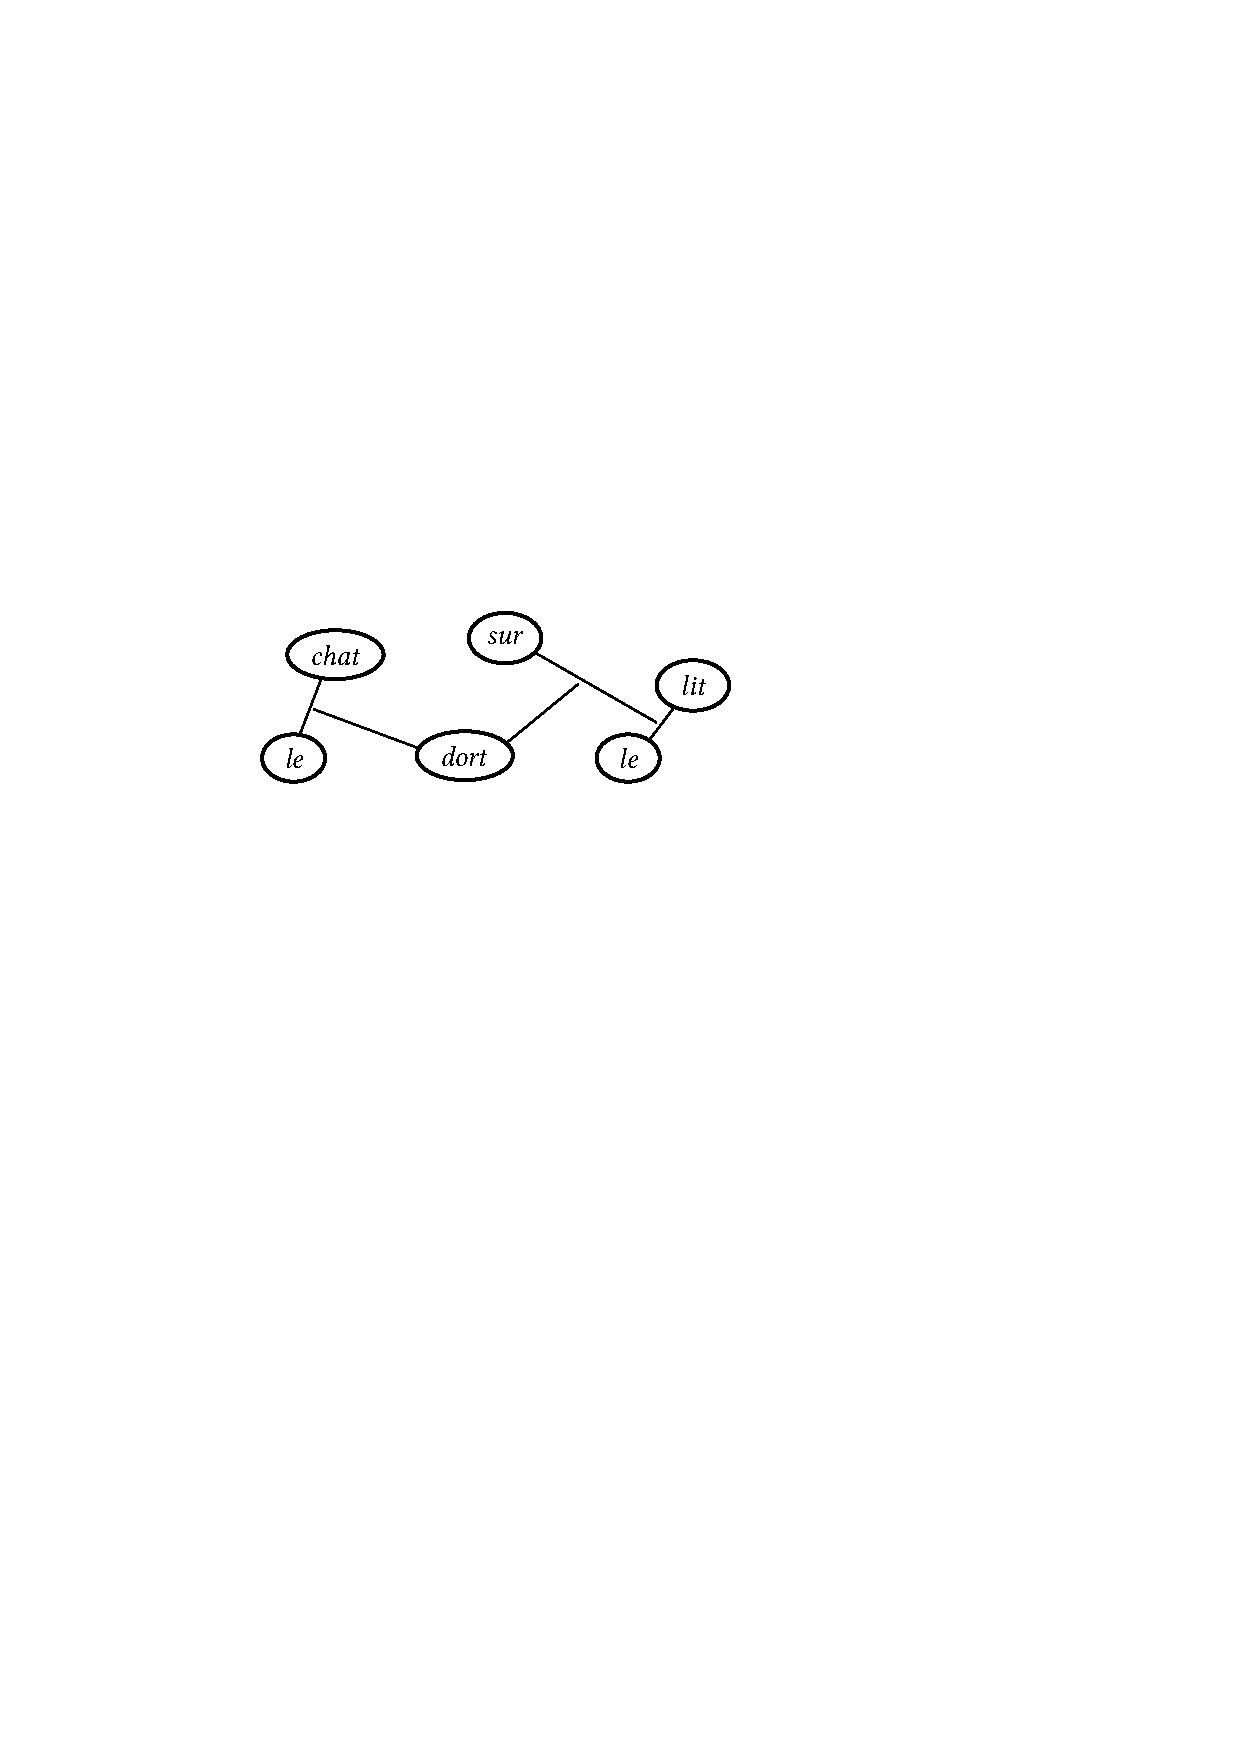
\includegraphics[scale=.75]{lechatdortsurlelit.pdf}
% %     \begin{tikzpicture}
% %       \matrix (matrix) [matrix of nodes,
% %                         nodes={ConcSet},
% %                         row sep=1em, 
% %                         column sep=1em,
% %                         ampersand replacement=\&]
% %         {
% %           \& chat \& \& sur \& \& lit\\
% %           le \& \& dort \& \& le \& \\
% %         };
% %       \coordinate (intersection1) at ( $ (matrix-2-1) !.5! (matrix-1-2) $ );
% %       \coordinate (intersection2) at ( $ (matrix-2-5) !.5! (matrix-1-6) $ );
% %       \coordinate (intersection3) at ( $ (matrix-1-4) !.5! (intersection2) $ );
% %       \draw (matrix-2-1)    -- (matrix-1-2);
% %       \draw (intersection1) -- (matrix-2-3)
% %                             -- (intersection3);
% %       \draw (matrix-1-4)    -- (intersection2);
% %       \draw (matrix-1-6)    -- (matrix-2-5);
% %     \end{tikzpicture}
    \end{center}

    Cette structure est donnée sous forme de polygraphe (voir \encadref{sec:3.2.23}).
    
    \begin{enumerate}[label=\alph*.]
    \item Quelles sont les unités qu’on peut déduire de cette structure ?
    \item À quels critères répond cette structure de connexion ?
    \item Peut-on raffiner les connexions de cette structure ? En utilisant quels critères ?
    \end{enumerate} 
}
\lecturesadditionnelles{%\label{sec:3.2.28}
    L’organisation de nos chapitres doit beaucoup aux travaux d’Igor Mel’čuk et nottament son ouvrage de \citeyear{melcuk1988dependency}. Celui-ci considère trois types de critères pour définir la structure syntaxique : les critères A décident si deux mots se combinent entre eux, les critères B lequel des deux mots est la tête du syntagme qu’ils forment, les critères C quelle est la relation qui les unit. Le présent chapitre est ainsi consacré aux combinaisons et donc aux critères A. Nous avons étendu l’analyse de Mel’čuk en ne limitant pas la connexion aux combinaisons de mots. Les critères B seront étudiés au \chapref{sec:3.3} sur \textit{Tête et dépendance}. Les critères C seront abordés plus tard, dans le \chapfuturef{18} sur \textit{Les relations syntaxiques.}

    L’autonomisabilité prosodique~et plus généralement la relation entre une structure de dépendances syntaxique et la structure prosodique a été étudiée par Piet Mertens dans sa thèse en \citeyear{mertens1987lintonation}. Pour un travail plus récent, on pourra consulter son article de \citeyear{mertens2008syntaxe}. Pour un travail précurseur sur les liens entre prosodie et syntaxe de dépendance, citons le travail d’Henri \citet{weil1844de} sur lequel nous reviendrons. \citet{lacheret1999prosodie} propose une présentation de la \textit{Prosodie du français}.

    Lucien Tesnière utilise des bulles dans ses représentations syntaxiques. Une formalisation des arbres à bulles est proposée par \citet{kahane1997bubble}. La définition de la structure de connexion par raffinement d’une fragmentation est proposée par \citet{gerdes2011defining}. La définition de la connexion comme une classe d’équivalence de combinaisons est développée dans \citet{kahane2018une}. Le lien historique entre connexion et analyse en constituants immédiats, chez Henry A. Gleason comme chez ses prédécesseurs, est étudié par \citet{mazziotta2017what}. Timothy Osborne a consacré plusieurs articles aux catenae ;  voir par exemple l'article de \citeyear{osborne2012catenae:} et son ouvrage de \citeyear{osborne2019dependency}.

    Sur le traitement cognitif de la syntaxe, on consultera les travaux précurseurs de Janet D. Fodor et de son étudiante Lyn Frazier. Dans leur article de \citeyear{frazier1978sausage}, elles défendent l’idée que les énoncés sont traités par petits paquets d’environ six mots qui sont ensuite connectés entre eux. Cette étude est suivie en \citeyear{frazier1982making} et \citeyear{fodor1994diagnosis} d’une analyse du traitement des phrases avec garden-path par l’analyse des mouvements oculaires, où il est défendu que l’énoncé n’est pas réanalysé, mais que le destinataire répare sa première analyse après avoir identifié la source de l’erreur.
    
    \FurtherReading{3-2}
}
\citations{%\label{sec:3.2.29}
    \noindent{\sffamily\bfseries Citations de la \sectref{sec:3.2.25}.}

    \noindent \citet[129--130]{gleason1955introduction} :

    \begin{quote}
    We may, as a first hypothesis, consider that each of [the words of the considered utterance] has some statable relationships to each other word. If we can describe these interrelationships completely, we will have described the syntax of the utterance in its entirety. […] We might start by marking those pairs of words which are felt to have the closest relationship.~[…]~We will also lay down the rule that each word can be marked as a member of only one such pair.~
    \end{quote}
}
\corrections{%\label{sec:3.2.30}
\corrigé{1} 
\begin{enumerate}[label=\alph*.]
\item Dans le premier cas, \textit{rapide} se combine avec la locution nominale \textit{coup d’œil}, ce qui explique la réalisation comme adjectif. Dans le deuxième cas, la combinaison a lieu avec le verbe \textsc{regarder}, ce qui entraine la réalisation par l’adverbe \textit{rapidement}.

\item Dans le premier cas, \textit{une épée} est le complément d’objet direct de la forme infinitive du verbe \textsc{manier}. Dans le deuxième cas, \textit{une épée} est le complément du nom \textit{maniement~}; dans ce cas, \textit{une épée} doit d’abord se combiner avec la préposition \textsc{de} avant de se combiner avec \textit{maniement}.
\end{enumerate}

\corrigé{2} Les deux positions acceptent des groupes substantivaux, des infinitives (\textit{lire le soir}) et des propositions complétive (\textit{qu’il pleuve le matin}). On observe deux différences dans les paradigmes. D’une part, les pronoms sujets et objets sont différents : \textit{\textbf{il} plaît à Marie} vs \textit{Marie} \textbf{\textit{l’}}\textit{aime}. D’autre part, la position sujet accepte des infinitives en \textit{de~}: \textit{\textbf{De lire le soir} plaît à Marie} vs *\textit{Marie aime de lire le soir}.

\corrigé{3} Les unités syntaxiques autonomisables de cet énoncé sont :

\begin{itemize}
\item les 8 mots : \textit{cet, étudiant, veut, acheter, un, livre, de, syntaxe~};
\item 4 segments de deux mots : \textit{cet étudiant, veut acheter, un livre, de syntaxe~};
\item 3 segments de trois mots : \textit{cet étudiant veut, acheter un livre, livre de syntaxe~};
\item 3 segments de quatre mots : \textit{cet étudiant veut acheter, veut acheter un livre, un livre de syntaxe~};
\item 1 segment de cinq mots : \textit{acheter un livre de syntaxe~};
\item 2 segments de six mots : \textit{cet étudiant veut acheter un livre, veut acheter un livre de syntaxe~};
\item l’énoncé complet : \textit{cet étudiant veut acheter un livre de syntaxe}.
\end{itemize}

\corrigé{4} 
\begin{enumerate}[label=\alph*.]
\item \textit{bien des années plus tard} forme un syntagme, puisqu’il peut être la réponse à la question «~\textit{Ca a commencé quand} ?~». À la même question, on peut répondre \textit{des années plus tard}, \textit{bien plus tard} ou \textit{plus tard}, voire juste \textit{tard}, mais pas \textit{bien des années}, \textit{bien}, \textit{des années} ou \textit{plus}. On en déduit que \textit{bien} et \textit{des années} se combinent avec \textit{plus tard}. Il est plus difficile de déterminer si \textit{bien} et \textit{des années} se combinent avec \textit{plus} ou \textit{tard}, puisque ni \textit{des années plus}, ni \textit{des années tard} n’est acceptable. On peut néanmoins remarquer qu’on trouve un groupe substantival avec \textit{plus} dans d’autres contextes : \textit{Il habite un étage plus haut~}; \textit{Fais-le deux centimètres plus large}. Par contre, on ne peut jamais combiner un groupe substantival avec \textit{tard} sans la présence de \textit{plus}, ce qui nous permet de conclure que \textit{des années} se combine avec \textit{plus}. Si \textit{bien} peut se combiner aussi bien avec \textit{plus} que \textit{tard}, il semble, au vu du sens, que c’est avec \textit{plus} qu’il se combine ici.
   

\begin{center}
\begin{tikzpicture}[every node/.style={font=\footnotesize,inner sep=1pt}]
 \node at (0,0) (A) [draw,circle,font=\itshape\strut] {ça};
 \node [right=1em of A] (B) [draw,circle,font=\itshape\strut] {a};
 \node [right=1em of B] (C) [ConcSet] {commencé};
 \node [right=1em of C] (D) [ConcSet] {tard};
 \node [right=1em of D] (E) [ConcSet] {plus};
 \node [above right=\baselineskip and 1em of E] (F) [ConcSet] {des};
 \node [right=1em of F] (G) [ConcSet] {années};
 \node [below right=\baselineskip and 1em of E] (H) [ConcSet] {bien};
 
 \node [fit = (F) (G),draw,ellipse,inner sep=0pt] (FG) {};
 \draw (A) -- (B) -- (C) -- (D) -- (E) -- (FG);
 \draw (F) -- (G);
 \draw (E) -- (H);
\end{tikzpicture}
\end{center}


\item La fragmentation du syntagme \textit{le plus haut mur du monde} pose plusieurs problèmes. Nous avons déjà traité le cas des adjectifs épithètes et expliqué pourquoi \textit{le haut} n’est pas un fragment acceptable. Mais c’est plus compliqué avec \textit{le plus haut}, puisqu’on a \textit{le mur le plus haut}. On peut argumenter que \textit{le} dans \textit{le plus haut mur} est bien l’article, car il commute avec un possessif : \textit{son plus haut mur}, \textit{mon plus vieil ami}. Ce qui n’est pas le cas qu’en \textit{le plus haut} forme une unité syntaxique et un groupe adjectival postposé au nom : *\textit{le mur notre plus haut}. On aurait donc la structure de connexion suivante pour \textit{le plus haut mur} :

\begin{center}
\begin{tikzpicture}
\matrix (matrix) [matrix of nodes, 
                  nodes = {ConcSet, minimum width=3em},
                  ampersand replacement=\&,
                  row sep=1em,
                  column sep=.33em,
                  inner sep = 0pt,
                  font=\small]
  { \& haut \& \& mur\\
      plus \& \& le\\  
  };
\draw (matrix-2-1) -- (matrix-1-2) -- (matrix-1-4) -- (matrix-2-3);
\end{tikzpicture}
\end{center}

Mais on peut aussi accepter que dans cette construction \textit{le} joue un double rôle : à la fois article défini (\textit{le mur}) et marqueur du superlatif (le plus), ce qui donne une structure cyclique.

\begin{center}
\begin{tikzpicture}
\matrix (matrix) [matrix of nodes, 
                  nodes = {ConcSet, minimum width=3em},
                  ampersand replacement=\&,
                  row sep=1em,
                  column sep=.33em,
                  inner sep = 0pt,
                  font=\small] 
  {
    \& haut \& \& mur\\
    plus \& \& le\\
  };
\draw (matrix-2-1) -- (matrix-1-2) -- (matrix-1-4) -- (matrix-2-3) -- (matrix-2-1);
\end{tikzpicture}
\end{center}

%%[Warning: Draw object ignored]
%%[Warning: Draw object ignored]


Un autre problème d’analyse vient du modifieur \textit{du monde}. Il ne s’agit pas d’un complément du nom \textit{mur}, puisque \#\textit{mur du monde}, s’il est acceptable, n’a pas le sens requis et surtout on a \textit{le mur le plus haut du monde}. De même, \textit{du monde} n’est pas un modifieur de l’adjectif, car l’absence du superlatif donne un sens inapproprié : \#\textit{le haut mur du monde}. Donc, bien que le fragment \textit{le plus du monde} soit inacceptable, nous pouvons considérer que la présence du modifieur du monde est validé par la présence du superlatif et que les deux sont donc connectés.
\end{enumerate}

\corrigé{5} 
\begin{enumerate}[label=\alph*.]
\item Les unités induites sont les mots, ainsi que \textit{le lit, sur le lit, le chat, le chat dort, dort sur le lit} et la phrase entière.
\item Ces unités obéissent aux critères d’autonomisabilité. En particulier, \textit{sur} ne peut apparaître sans son complément \textit{le lit}.
\item On peut raffiner la structure en utilisant le critère distributionnel. Nous verrons au chapitre suivant qu’il y a de bonnes raisons de considérer la combinaison \textit{dort} \textrm{${\oplus}$} \textit{sur}. Il est moins facile de raffiner les connexions mettant en jeu une unité déterminant-nom comme \textit{le chat} ou \textit{le lit}.
\end{enumerate}}

\chapter{\gkchapter{Tête et dépendance}{Hiérarchiser la structure syntaxique}}\label{sec:3.3}

\section{Hiérarchie}\label{sec:3.3.0}

Les syntaxèmes, mots et autres unités syntaxiques ne sont pas seulement connectés les uns aux autres : certains dominent les autres et leur imposent leurs propriétés syntaxiques (catégorie, forme, fonction, place). Nous avons largement argumenté l’existence d’une structure syntaxique hiérarchique lorsque nous avons étudié les exemples \textit{Pierre a été malade pendant deux semaines} et \textit{La maladie de Pierre a duré deux semaines} dans le \chapref{sec:1.2}. Nous renvoyons le lecteur à cette discussion. De nouveaux éléments seront donnés dans la suite de ce chapitre. En particulier :

\begin{itemize}
\item les contraintes distributionnelles ;
\item la rection ;
\item la hiérarchie sémantique ;
\item les contraintes sur l’ordre des mots.
\end{itemize}

Avant cela, nous allons introduire un peu de terminologie, en nous basant sur la notion de connexion, introduite au chapitre précédent.

\section{Tête et dépendance}\label{sec:3.3.1}

La hiérarchie de la structure syntaxique se traduit par une asymétrie des combinaisons entre unités, lesquelles combinent alors une unité hiérarchiquement supérieure à une unité qui lui est assujettie.

\Definition{\textstyleTermes{dépendance}}
{Une \textbf{connexion hiérarchisée} est appelée une \textstyleTermes{dépendance}.}

\Definition{\textstyleTermes{gouverneur}, \textstyleTermes{dépendant}}
{Si A et B sont connectés et que A est hiérarchiquement supérieur à B, on dit que A \textstyleTermes{gouverne} B et que B \textstyleTermes{dépend} de A. Ou encore que A est le \textstyleTermes{gouverneur} de B et que B est un \textstyleTermes{dépendant} de A. En général, un élément peut avoir un nombre quelconque de dépendants, mais il n’a qu’un seul gouverneur.}

En syntaxe de dépendance, depuis les travaux fondateurs de Lucien Tesnière, les dépendances syntaxiques lient des mots entre eux. Dans notre approche, les dépendances, comme les connexions, peuvent être considérées entre n’importe quelles unités syntaxiques et une même dépendance peut être décrite de façon plus ou moins fine en l’attribuant à des unités syntaxiques plus ou moins larges (voir la \sectref{sec:3.2.14} sur \textit{La connexion et ses instances}). Nous manipulerons des structures de granularité variable : parfois les mots seront les nœuds de la structure, mais parfois nous considérerons des unités plus fines (les syntaxèmes) ou des unités plus larges (voir la \sectref{sec:3.2.18} sur \textit{Structures de connexion, granularité et critères} et la \sectref{sec:3.4.1} sur l’\textit{Arbre de Beauzée-Gladkij}).

Une dépendance est représentée par une \textbf{flèche} qui va \textbf{du gouverneur vers le dépendant} ou encore simplement en positionnant le \textbf{gouverneur au dessus du dépendant}. Nous illustrons cela avec l’énoncé \textit{Marie parle} où le verbe \textit{parle} gouverne \textit{Marie}.

\begin{figure}
%%[Warning: Draw object ignored]
\begin{tikzpicture} [every node/.style={font=\strut}]
  \matrix [row sep=1em, column sep=.75em] (matrix)
    {
      \node (parle) [ConcSet] {parle}; & \node {gouverneur};\\
      \node (Marie) [ConcSet] {Marie}; & \node {dépendant};\\
    };
  \draw (parle) -- (Marie);
\end{tikzpicture}\hspace{2cm}
\begin{tikzpicture}[every node/.style={font=\strut}]
  \matrix [row sep=.5em, column sep=1em] (matrix)
    {
      \node (Marie) [ConcSet] {Marie}; & \node (parle) [ConcSet] {parle};\\
       \node {dépendant}; & \node {gouverneur};\\
    };
\draw[-{Triangle[]}] (parle) to [bend right] (Marie);
\end{tikzpicture}
\caption{\label{fig:}Deux représentations d’une dépendance}
\end{figure}

Le sens de la flèche, du gouverneur vers le dépendant, est une convention. Comme toute convention, elle est en partie arbitraire. Il aurait été tout à fait possible d’orienter les flèches dans l’autre sens, comme certains auteurs l’ont fait. Nous adoptons ici la convention qui est la plus largement répandue.

La représentation avec le gouverneur au dessus est également arbitraire, même si l’on est largement habitué aujourd’hui à une telle représentation de la hiérarchie (voir par exemple l’organigramme des responsabilités dans une entreprise). Dans ses premiers schémas en \citeyear{tesniere1934comment}, Tesnière adoptait une autre convention : il plaçait l’élément dominant au centre comme le soleil au centre du système solaire (voir l’\encadref{fig:3.3.5} sur l’\textit{Historique des représentations syntaxique par des diagrammes en dépendance}).

Nous allons introduire un autre terme à ne pas confondre avec \textit{gouverneur}.

\Definition{\textstyleTermes{tête d'une unité syntaxique}}
{On appelle \textstyleTermes{tête} d’une unité syntaxique U toute sous-unité de U qui n’est gouvernée par aucune autre sous-unité de U.}

Les notions de tête et de gouverneur renvoient au même concept, mais adopte des points de vue différents.

\Definition{\textstyleTermes{dépendant}, \textstyleTermes{gouverneur}}
{Si A et B forment à eux deux une unité syntaxique dont A est la \textbf{tête}, alors A est le \textstyleTermes{gouverneur} B. Inversement, si A est le \textstyleTermes{gouverneur} B, alors A et B forment une unité syntaxique ensemble et A en est la \textbf{tête}. Enfin, B est le \textstyleTermes{dépendant} de A si et seulement si A est le \textstyleTermes{gouverneur} B.}

Autrement dit, hiérarchiser une connexion revient donc à décider de quel côté est sa tête.

On aura noté que pour une unité syntaxique U donnée, \textbf{la tête de U est un élément de U}, en quelque sorte l’élément le plus important de U du point de vue de la syntaxe, tandis que \textbf{le gouverneur de U est un élément extérieur à U}. (On peut se souvenir, pour ne pas confondre les deux termes, que la tête d’une personne fait toujours partie de cette personne.) Illustrons ces notions avec \textit{une très jolie valise} et U = \textit{très jolie}. La tête de U est \textit{jolie}, tandis que le gouverneur de U est \textit{valise}.

\begin{figure}
\begin{tikzpicture}[every pin edge/.style={dashed,lsDOIGray}]
\node at (0,0) [ConcSet,pin=west:{gouverneur de U}] (valise) {valise};
\node at (0,-2) [ConcSet,pin=east:{tête de U}] (jolie) {jolie};
\node at (0,-4) [ConcSet] (tres) {très};
\draw (valise) -- (jolie) -- (tres);
\node [fit=(tres) (jolie), draw, ellipse, inner sep=0pt,pin=west:U] {};
\end{tikzpicture}
  \caption{\label{fig:}Gouverneur vs. tête}
\end{figure}

Les grammaires de dépendance traditionnelles font l’hypothèse que toute unité possède un unique mot tête. Nous considérons pour notre part que la nature de la tête dépend de la granularité de l’analyse et qu’on peut considérer, selon les finalités de l’analyse, une unité plus fine que le mot (un syntaxème) comme une unité plus large. Par ailleurs, il peut arriver que plusieurs éléments possèdent des propriétés de tête : on parle alors de \textstyleTermes{co-têtes} (voir la \sectref{sec:3.3.27} sur \textit{Nom et déterminant comme co-têtes}).

Concluons cette section en soulignant une propriété fondamentale que nous exploiterons pour identifier la tête d’une unité : le \textbf{gouverneur} d’une unité U est \textbf{connecté à la tête} de U.

\chevalier{Historique des notions de dépendance et de tête}{%\label{sec:3.3.2}
    Le premier grammairien à utiliser le terme «~dépendance~» dans un sens grammatical est semble-t-il un grammairien arabe, \textbf{Ibn Mada}, qui vécut en Espagne (alors sous domination arabe) entre 1119 et 1195. Il est connu pour son livre, intitulé \textit{La réfutation des grammairiens}, dans lequel il s’attaque à des sujets qui sont toujours d’actualité. Il critique l’utilisation de formes invisibles sous-jacentes et notamment l’introduction d’un morphème zéro pour le nominatif. Il se prononce aussi en faveur d’une indépendance de la syntaxe et de la sémantique et contre une justification sémantique ou une interprétation cognitive des règles grammaticales : «~Et pourquoi l’agent est-il au nominatif ? La réponse correcte est […] que c’est ainsi que parlent les Arabes.~» Comme nous l’avons dit, il utilise le terme {\arfont تعلق} \textit{ta’alluq}, qui se traduit par \textit{être accroché à, dépendre de, être connecté à, joindre, attachement, amour du monde, dépendance, connexion, relation,} et même \textit{obsession.} Il préfère ce terme à {\arfont عمل} \textit{\textsuperscript{c}}\textit{amal} ‘opération, gouverner’, le terme utilisé communément à son époque en grammaire pour décrire des relations entre le gouverneur et le dépendant. Selon Ibn Mada, le gouverneur n’opère pas sur ses dépendants, il y a seulement une relation, une dépendance. Il va même jusqu’à appeler hérétique toute utilisation de \textit{\textsuperscript{c}}\textit{amal} car, selon lui, des mots ne peuvent agir sur d’autres mots et déclencher une flexion. Comme l’utilisation de \textit{ta’alluq} était essentiellement un changement terminologique pour une notion établie de longue date sous le terme de \textit{\textsuperscript{c}}\textit{amal}, le terme de \textit{dépendance} n’a pas vraiment pris avant le 20\textsuperscript{e} siècle et les travaux de Lucien Tesnière, qui lui donnaient une assise théorique forte (bien que Tesnière lui-même utilise le terme de connexion).

    L’importance d’une analyse de type dépendentiel pour la description de phénomènes grammaticaux, par contre, était établie bien avant Ibn Mada. On attribue généralement à \textbf{Sibawayh}, le grand grammairien perse travaillant sur l’arabe, la première modélisation grammaticale en termes de dépendances entre mots et notamment en ce qui concerne l’attribution des cas aux noms dépendant d’un verbe. Sibawayh a vécu de 760 à 796 et on raconte qu’il est mort, très jeune, de la fureur qui l’a saisi lors d’un débat sur la grammaire de l’arabe (premier accident de travail d’un linguiste {\CryingSmiley}). Il est le fondateur d’une tradition grammaticale qui reste aujourd’hui vivace.

    Avant l’avènement de la tradition grammaticale arabe, on analysait déjà la structure des phrases en faisant référence à des liens hiérarchisés entre les mots. La plus vieille grammaire étendue qu’on connaît, les descriptions du sanskrit par l’immense linguiste indien \textbf{Pāṇini} au 4\textsuperscript{e} siècle avant notre ère, introduit la notion de \textit{karaka} pour désigner les relations entre verbes et noms, qui sont classées en six classes différentes en se basant sur des critères sémantiques autant que syntaxiques. Parmi ces classes de liens, on trouve déjà l’agent/sujet (\textit{karta}) et le patient/objet (\textit{karma}). Il faudra de toute façon attendre le 20\textsuperscript{e} siècle pour une distinction claire entre les notions syntaxiques de \textit{sujet} et \textit{objet} d’une part et les notions sémantiques d’\textit{agent} et de \textit{patient} d’autre part (voir l’encadré sur \textit{Sujet, agent, thème} au \chapfuturef{18}).

    Généralement, on constate qu’une analyse en termes de dépendances s’est imposée pour pratiquement toute analyse grammaticale jusqu’à l’apparition des grammaires de constituants au 20\textsuperscript{e} siècle, en particulier pour des langues flexionnelles et à ordre libre, comme le sanskrit, l’arabe ou encore l’allemand.

    L’idée d’une analyse syntaxique complète d’un énoncé apparaît, à notre connaissance au début du 18\textsuperscript{e} siècle, en France. Il est probable que l’impulsion donnée au 17\textsuperscript{e} siècle par la parution de la \textit{Grammaire de} \textbf{\textit{Port-Royal}} (\citealt{ArnauldLancelot1660}), puis de la \textit{Logique de Port Royal} (\citealt{ArnauldNicole1662}) a été déterminante. En \citeyear{buffier1709grammaire} paraît la \textit{Grammaire françoise sur un plan nouveau} de \textbf{Claude Buffier} qui comprend plusieurs analyses très élaborées. Malgré le caractère très moderne de ses analyses, Buffier reste relativement peu connu, probablement en raison d’une terminologie qui ne distingue pas clairement les relations syntaxiques de la morphologie. Si l’on remplace, dans les citations qui suivent, \textit{régime} par \textit{complément} ou \textit{dépendant}, on voit que les analyses de Buffier sont de parfaites analyses en dépendance : «~Tous les noms ou même tous les mots qui servent ainsi à particulariser la signification d’un autre mot, sont le régime de ce mot : comme si je dis \textit{un ami de plaisir}, la signification d’\textit{un ami} est particularisée par le mot \textit{de plaisir~}; c’est pourquoi \textit{de plaisir} est le régime d’\textit{un ami}. » (p. 57) « \textit{Dieu agit avec justice. Avec} est un mot qui n’a point de sens déterminé et complet par lui-même ; mais par le mot \textit{justice} dont il est ici suivi et qui en est le régime.~» (p. 73) Les analyses de Buffier, comme celles qui suivront tout au long du 18\textsuperscript{e} siècle, sont données de manière discursive (c’est-à-dire sans schéma), ce qui les rend plus difficiles à saisir. Nous nous proposons d’en étudier une en détail dans l'exercice 1 à la fin de ce chapitre.

    Dans son ouvrage de \citeyear{girad1747vrais}, \textit{Les Vrais principes de la langue françoise, ou la Parole réduite en méthode}, l’abbé \textbf{Gabriel Girard} utilise le terme \textit{dépendance} dans un sens compatible avec la définition moderne : «~J’abandonne toutes les observations qu’on pourrait faire sur le Style, pour me borner uniquement à ce qui regarde l’union grammaticale des mots. Cette sorte d’union établit entre eux un RÉGIME, qui est très distingué de ce que je viens de nommer style ; ce dernier consistant dans des rapports de convenance [= relation d’accord] dont le goût fait choix pour la conduite du discours, et l’autre dans des rapports de dépendance soumis aux règles pour la construction de la phrase.~» (p. 87, nous modernisons l’orthographe) Mais Girard préfère néanmoins parler de régime plutôt que de dépendance : «~Le Régime n’est autre chose que le concours des mots pour les expressions d’un sens ou d’une pensée. Dans ce concours de mots il y en a qui tiennent le haut bout ; ils en régissent d’autres, c’est-à-dire qu’ils les assujettissent à certaines lois : il y en a qui se présentent d’un air soumis ; ils sont \textit{régis} ou tenus de se conformer à l’état et aux lois des autres ; et il y en a qui sans être assujettis ni assujettir d’autres, n’ont de lois à observer que celle de la place dans l’arrangement général.~» (p. 87) (L’idée, exprimée à la fin de cette citation, qu’il y a des mots qui n’entrent pas dans la rection, sera reprise par l’Approche pronominale et conduira à la distinction entre micro et macrosyntaxe ; voir partie 6.)

    \textbf{Nicolas Beauzée}, dans l’article «~Régime~» de l’\textit{Encyclopédie} (\citeyear{Beauzée1765}), va introduire la distinction entre la notion de \textit{complément} et le régime proprement dit (c’est-à-dire «~la forme particulière que doit prendre un complément grammatical d’un mot, en conséquence du rapport particulier sous lequel il est alors envisagé~»), critiquant au passage l’emploi du terme \textit{régime} par Girard. Beauzée est ainsi le premier à distinguer clairement \textbf{dépendance syntaxique} et \textbf{dépendance morphologique} (voir encadré suivant). Beauzée ne dessine pas de diagramme, mais il fait une description détaillée de la structure syntaxique qui est similaire aux diagrammes que proposera Aleksej Gladkij plus de deux siècles plus tard (\citeyear{gladkij1968describing}), diagrammes que nous appellerons pour cette raison des arbres de Beauzée-Gladkij (voir \sectref{sec:3.4.1} \textit{Arbre de Beauzée-Gladkij}) : «~Par exemple, dans cette phrase, \textit{nous avons à vivre avec des hommes semblables à nous :} ce dernier \textit{nous} est le \textit{complément} de la préposition \textit{à ; à nous} est celui de l’adjectif \textit{semblables ; semblables à nous} est le \textit{complément} total du nom appellatif \textit{les hommes ; les hommes semblables à nous}, c’est la totalité du \textit{complément} de la préposition \textit{de}.~»

    Mieux encore, Beauzée distingue le \textit{complément grammatical} ou \textit{initial}, qui est un mot, du \textit{complément logique} ou \textit{total}, qui en est la projection (voir \sectref{sec:3.3.30} \textit{Dominance et projections maximales}), montrant ainsi le passage d’un arbre de Beauzée-Gladkij à un arbre de dépendance (que nous détaillerons tout au long du \chapref{sec:3.4}) : «~Par exemple, dans cette phrase, \textit{avec les soins requis dans les circonstances de cette nature ;} le mot \textit{nature} est le \textit{complément} grammatical de la préposition \textit{de : cette nature} en est le \textit{complément} logique : la préposition \textit{de} est le \textit{complément} initial du nom appellatif \textit{les circonstances ;} et \textit{de cette nature} en est le \textit{complément} total : \textit{les circonstances}, voilà le \textit{complément} grammatical de la préposition \textit{dans ;} et \textit{les circonstances de cette nature} en est le \textit{complément} logique.~» Il faut néanmoins remarquer que le sujet n’est pas considéré comme un dépendant du verbe, ce que souligne le choix même du terme \textit{complément} (voir la discussion dans le \chapfuturef{18}). Beauzée énonce même la \textbf{projectivité} (voir la \sectref{sec:3.5.14} sur la \textit{Projectivité}), notant que les compléments logiques/totaux tendent à être continues.

    On peut considérer que Beauzée est le premier linguiste à donner une description claire d’une structure de dépendance. Cette description est faite à base de mots et ne trouve pas encore de traduction graphique, mais elle n’en reste pas moins une véritable analyse en dépendance. Cette opinion converge avec celle de Jean-Claude Chevalier, qui considère dans son monumental ouvrage de \citeyear{chevalier1968histoire} sur l’histoire de la syntaxe de 1530 à 1750 qu’avec Beauzée s’achève la définition de la notion actuelle de \textbf{complément}.

    Les idées de Beauzée doivent beaucoup à celles de \textbf{Dumarsais} qui rédigea onze ans plus tôt l’article «~Construction~» de l’\textit{Encyclopédie} (\citeyear{Dumarsais1754}). Dans cet article, Dumarsais décrit la dépendance en utilisant le terme \textit{détermination} : «~Un mot doit être suivi d’un ou de plusieurs autres mots déterminants, toutes les fois que par lui-même il ne fait qu’une partie de l’analyse d’un sens particulier ; l’esprit se trouve alors dans la nécessité d’attendre et de demander le mot déterminant, pour avoir tout le sens particulier que le premier mot ne lui annonce qu’en partie. […] Quelqu’un me dit que \textit{le Roi a donné ;} ces mots \textit{a donné} ne font qu’une partie du sens particulier, l’esprit n’est pas satisfait, il n’est qu’ému, on attend, ou l’on demande, 1° \textit{ce que le Roi a donné,} 2° \textit{à qui il a donné.} On répond, par exemple, à la première question, que \textit{le Roi a donné un régiment :} voilà l’esprit satisfait par rapport à la chose donnée ; \textit{régiment} est donc à cet égard le déterminant de \textit{a donné,} il détermine \textit{a donné.} On demande ensuite, \textit{à qui le Roi a-t-il donné ce régiment} ? on répond \textit{à monsieur N.} ainsi la préposition \textit{à}, suivie du nom qui la détermine, fait un sens partiel qui est le déterminant de \textit{a donné}.~» (Voir l'exercice 2 pour une autre analyse de Dumarsais.)

    Sans que le terme \textit{complément} ne soit utilisé de façon aussi systématique, Dumarsais ébauche la distinction entre complément grammatical et complément logique qui sera ensuite élaborée par Beauzée et qui préfigure la distinction actuelle entre une analyse en dépendance et une analyse en constituants : «~On peut considérer une proposition ou grammaticalement ou logiquement : quand on considère une proposition grammaticalement, on n’a égard qu’aux rapports réciproques qui sont entre les mots ; au lieu que dans la proposition logique, on n’a égard qu’au sens total qui résulte de l’assemblage des mots.~»

    Enfin, on doit également à Dumarsais, l’idée reprise par Tesnière (voir la \sectref{sec:3.2.8} sur la \textit{Connexion}) que le sens naît des \textbf{connexions} entre les mots : «~Il faut d’abord établir comme un principe certain, que les mots n’ont entre eux de rapport grammatical, que pour concourir à former un sens dans la même proposition, et selon la construction pleine ; car enfin les terminaisons des mots et les autres signes que la Grammaire a trouvés établis en chaque langue, ne sont que des signes du rapport que l’esprit conçoit entre les mots, selon le sens particulier qu’on veut lui faire exprimer. Or dès que l’ensemble des mots énonce un sens, il fait une proposition ou une énonciation. Ainsi celui qui veut faire entendre la raison grammaticale de quelque phrase, doit commencer par ranger les mots selon l’ordre successif de leurs rapports, par lesquels seuls on aperçoit, après que la phrase est finie, comment chaque mot concourt à former le sens total.~» (article «~Concordance~», \textit{Encyclopédie}, \citeyear{Dumarsais1753}).

    L’idée d’une hiérarchie est également développée par l’abbé \textbf{Roch-Amboise} \textbf{Sicard}, qui dans son ouvrage de \citeyear{sicard1801elemens}, \textit{Élémens de grammaire générale appliqués à la langue française}, présente sa \textbf{théorie du chiffre~}: «~On désigne certaines prépositions par le chiffre 4, et leur complément, par le chiffre 5.~» (p. 106), mais le sujet est considéré comme dominant le verbe : «~On désigne le sujet par le chiffre 1, qui est censé être l’expression d’une moitié de l‘\textit{unité}. On désigne la qualité [= l’objet] par le même chiffre, qui représente l’autre moitié de la même \textit{unité}. On désigne le mot-lien, qui est le verbe, par le chiffre 2.~» (p. 105).

    La théorie du chiffre de Sicard semble avoir été reprise par le grammairien américain \textbf{James Brown}, puis par le linguiste danois \textbf{Otto Jespersen}, qui en a fait une \textbf{théorie des rangs}, dont le verbe est absent ! Jespersen, qui a eu une grande influence sur ses contemporains, et notamment Tesnière, écrit dans \textit{The Philosophy of Language} en \citeyear{jespersen1924philosophy} (chapitre VII) : «~Dans toute dénomination composite d’une chose ou d’une personne, nous voyons toujours qu’il y a un mot d’importance suprême auquel les autres sont joints ou subordonnés. Ce mot principal est défini (qualifié, modifié) par un autre mot, qui à son tour est défini (qualifié, modifié) par un troisième mot, etc. Nous sommes ainsi amenés à établir différents «~rangs~» de mots selon leurs relations mutuelles comme défini ou définissant. Dans la combinaison (\textit{un}) \textit{temps extrêmement chaud}, le mot \textit{temps}, qui est évidemment l’idée principale, peut être appelé primaire ; \textit{chaud}, qui définit \textit{temps}, secondaire ; et \textit{extrêmement}, qui définit \textit{chaud}, tertiaire.~» Jespersen va appliquer sa théorie des rangs à une analyse formelle d’un grand nombre d’exemples dans \textit{Analytic Syntax} publié en 1937. Par exemple, \textit{It will learn it soon enough} ‘Il va apprendre ça suffisamment tôt’ est analysé S V O 3 4, indiquant ainsi que \textit{enough}\textsubscript{4} modifie \textit{soon}\textsubscript{3}.

    L’existence d’une hiérarchie s’est également exprimée à travers la notion de \textbf{tête} (angl. \textit{head}), dont on peut faire remonter l’introduction au grammairien anglais \textbf{Henry Sweet} (\citeyear{sweet1891new}, \textit{A new English Grammar}, sections 40 and 41) : «~\textbf{40}. La relation la plus générale entre des mots dans une phrase est, du point de vue logique, celle de \textbf{mot-ajout} et \textbf{mot-tête}, ou, comme on peut aussi dire, de \textbf{modifieur} et \textbf{modifié}. Ainsi dans les phrases \textit{les hommes grands ne sont pas toujours forts, tous les hommes ne sont pas forts, grand, fort} et \textit{tous} sont des mots-ajouts modifiant le sens du mot-tête \textit{hommes}. De même \textit{foncé, rapide, rapidement} sont des mots-ajouts dans \textit{rouge foncé, il a un pas rapide, il marche rapidement}. \textit{Stone} ‘pierre’ est un mot-ajout dans \textit{stone wall, wall of stone}, parce qu’il modife (défini) le sens de \textit{wall} ‘mur’. De même, \textit{book} (\textit{books}) est un mot-ajout dans \textit{book-seller} ‘marchand de livres’, \textit{bookselling, sale of books} ‘vente de livres’, \textit{he sells books} ‘il vend des livres’, \textit{he sold his books} ‘il a vendu ses livres’, les mots-têtes correspondants étant \textit{seller, selling, sells, sold}.~» Comme on peut le voir dans cette citation suivante, Sweet bascule du concept de tête à celui de gouverneur : «~\textbf{41.} […] La distinction entre mot-ajout et mot-tête est seulement relative : un même mot peut être un mot-tête dans une phrase ou un contexte et un mot-ajout dans un autre, et un même mot peut être mot-tête et mot-ajout en même temps. Ainsi dans \textit{il est très fort}, \textit{fort} est un mot-ajout de \textit{il} et en même temps mot-tête du mot-ajout \textit{très}, lequel peut lui-même être un mot-tête, comme dans \textit{il est pas très fort}.~»

    L’équivalence entre les notions de tête et de dépendance est formellement montrée par \textbf{Yves Lecerf} dans un rapport de \citeyear{lecerf1960programme}. Cette équivalence est présentée en détail dans le \chapref{sec:3.4}.

    La première formalisation de la notion de tête revient probablement à \textbf{Leonard Bloomfield}. Dans sa grande œuvre, \textit{Langage}, publiée en \citeyear{bloomfield1933language} et considérée à juste titre comme l’ouvrage fondateur de la syntaxe de constituants, Bloomfield consacre davantage d’énergie à définir la notion de tête que celle de constituant. Il y distingue notamment les \textstyleTermesapprof{constructions endocentriques} (celles qui ont une tête) des \textstyleTermesapprof{constructions exocentriques} (celles qui n’en ont pas) : «~Toute construction syntaxique met en jeu deux (ou parfois plus) formes libres combinées en un syntagme (\textit{phrase}), que l’on peut appeler le syntagme \textit{résultant}. Le syntagme résultant peut n’appartenir à la classe distributionnelle (\textit{form-class}) d’aucun constituant. Par exemple, \textit{John ran} n’est ni une expression nominative (comme \textit{John}), ni une expression verbale finie (comme \textit{ran}). Par conséquent, nous dirons que la construction anglaise acteur-action est \textit{exocentrique} : le syntagme résultant n’appartient à la classe distributionnelle d’aucun constituent immédiat. Inversement, le syntagme résultant peut appartenir à la même classe distributionnelle que l’un (ou plus) des constituants. Par exemple, \textit{poor John} est une expression nominale propre, comme l’est le constituant \textit{John~}; les formes \textit{John} et \textit{poor John} ont, dans l’ensemble, les mêmes fonctions. En conséquence, nous dirons que la construction anglaise caractère-substance (comme dans \textit{poor John, fresh milk}, etc.) est une construction \textit{endocentrique}.~» On notera que la construction \textit{sujet-verbe} (appelée par Bloomfield \textit{actor-action}) est considérée comme exocentrique, une analyse qui s’est perpétuée depuis la \textit{Grammaire de Port Royal} (\citealt{ArnauldLancelot1660}) et qui va se maintenir dans les grammaires de constituants jusqu’à l’avènement de la syntaxe X-barre à la fin des années 1970 (voir \encadref{fig:3.4.19} sur la \textit{Syntaxe X-barre}).

    La «~\textstyleTermesapprof{centralité du verbe}~» et le fait que la relation sujet-verbe est exocentrique est, elle, défendue par le linguiste hongrois \textbf{Brassai} dès \citeyear{bra} : «~Assis au début, au milieu ou à la fin de la phrase, quel que soit l’endroit où il lui plaît d’être, se trouve le verbe, relié par des liens sémantiques à ses vassaux, les dépendants. […] L’autorité du verbe n’est pas dictatoriale et ses vassaux ne sont pas des esclaves, mais ont des relations légiférées avec leur seigneur et les uns avec les autres ; ils possèdent chacun un certain degré d’autonomie et un certain rang, avec un féodalisme dont le slogan, comme aux temps historiques, est \textit{nulle terre sans seigneur} [en français dans le texte].» (d’après une traduction en anglais du hongrois dans l’article \textit{Constituency or dependency? Notes on Sámuel Brassai’s syntactic model of Hungarian} d’András \cite{imrenyi2013constituency}).

    \textbf{Lucien Tesnière}, dès son article de \citeyear{tesniere1934comment}, défend avec véhémence la centralité du verbe : «~Une phrase se présente comme un système solaire. Au centre, un verbe qui commande tout l’organisme de même que le soleil est au centre du système solaire.~» Il insiste sur le fait que le sujet dépend du verbe comme les autres actants, considérant ainsi la combinaison \textit{sujet-verbe} comme endocentrique : «~L’opposition du sujet et du prédicat empêche ainsi de saisir l’équilibre structural de la phrase, puisqu’elle conduit à isoler comme sujet un des actants, à l’exclusion des autres, lesquels se trouvent rejetés dans le prédicat pêle-mêle avec le verbe et tous les circonstants. […] L’opposition du sujet et du prédicat masque en particulier le caractère interchangeable des actants, qui est à la base du mécanisme des voix actives et passive.~» (\citeyear{tesniere1959elements}: chapitre 49) (Le terme prédicat est à prendre ici dans un sens particulier dont nous discuterons à nouveau dans l’encadré \textit{Fonctions syntaxiques et prédicat} au \chapfuturef{18}.) Dans ses premiers diagrammes syntaxiques, Tesnière place le verbe au centre (voir \encadref{fig:3.3.5} \textit{Historique des représentations syntaxiques par des diagrammes en dépendance}).

    Premièrement, Tesnière n’a pas introduit le terme de \textit{dépendance}. Comme nous l’avons dit au chapitre précédent, Tesnière utilise le terme de \textbf{\textit{connexion}}, une connexion liant toujours pour lui un élément \textbf{régissant} à un élément \textbf{subordonné}. Quant à la structure qu’il associe à une phrase, il l’appelle un \textbf{stemma}. Deuxièmement, le stemma n’est pas un arbre de dépendance, mais une structure de dépendance dont certains liens ne sont pas hiérarchisés. À côté de la «~connexion~», qui est donc une dépendance chez lui, Tesnière considère deux autres types de relations syntaxiques, considérées comme exocentriques : la \textbf{translation} et la \textbf{jonction}. En conséquence, le stemma n’est pas non plus un graphe, puisqu’en cas de translation, le gouverneur de la translation a la translation complète pour dépendant et non l’un des éléments en relation de translation. Comme nous sommes sur des positions assez proches de Tesnière, nous aurons l’occasion de revenir sur la translation et la jonction et d’expliquer pourquoi il peut être envisagé de ne pas les considérer comme des relations hiérarchiques. La translation est discutée à la section sur \textit{La translation syntaxique} du \chapfuturef{17}. Quant à la jonction, elle fait l’objet d’un chapitre entier, le \chapfuturef{19}.

    L’idée que toutes les constructions sont endocentriques va être défendue plus tard, dans les années 1960--1970, aussi bien du côté de la syntaxe de dépendance avec l’école de Moscou (voir l’ouvrage d’\textbf{Igor Mel’čuk}, \textit{Dependency Syntax}, de 1988, qui reprend des travaux publiés en russe dans les années 1960--1970), que du côté de la syntaxe de constituants avec la syntaxe X-barre (voir l’ouvrage éponyme de \textbf{Ray Jackendoff} de 1977). On est ensuite revenu sur cette position en remarquant que, si l’on peut toujours se donner des critères pour attribuer une tête à chaque connexion (comme le fait Mel’čuk par exemple), il faut néanmoins reconnaître que ces critères ne s’appliquent pas de la même façon avec toutes les constructions et que dans un certain nombre de constructions un deuxième élément peut avoir des propriétés de tête. C’est la position que nous défendrons ici.

    Il faut aussi signaler que c’est seulement à partir de la fin des années 1970 que les linguistes vont répertorier de manière systématique les critères qui permettent de caractériser la tête (ou ce qui revient à peu près au même, la dépendance). On trouve des critères syntaxiques explicites pour définir la dépendance dans un article remarquable de \textbf{Paul Garde} de \citeyear{garde1977ordre} (voir discussion dans l’exercice 4) et une tentative de définition systématique de la dépendance dans l’ouvrage d’\textbf{Igor Mel’čuk} de \citeyear{melcuk1988dependency}. L’article d’\textbf{Arnold Zwicky} de \citeyear{zwicky1985heads}, intitulé \textit{Heads}, reste fameux pour avoir répertorié les différents critères de définition de la tête et montré comment ils coïncidaient ou non selon les constructions. \textbf{Richard Hudson} répond à Zwicky dans un article de \citeyear{hudson1987zwicky} en corrigeant certaines analyses et en montrant que les critères sont beaucoup plus convergents que ne le dit Zwicky.

    Nous poursuivons cette discussion dans l’\encadref{fig:3.3.5} consacré à l’\textit{Historique des représentations syntaxiques par des diagrammes en dépendance} et l’\encadref{fig:3.4.17} consacré à l’\textit{Historique des représentations syntaxiques par des diagrammes en constituants}.
}

\loupe{Dépendances morphologique, syntaxique et sémantique}{%\label{sec:3.3.3}
    Nous nous intéressons dans ce chapitre à la syntaxe et lorsque nous parlons de dépendance, il s’agit évidemment de \textstyleTermesapprof{dépendance syntaxique}. Igor Mel’čuk a contrasté cette notion avec celles de dépendances morphologique et sémantique.

    Les \textstyleTermesapprof{dépendances sémantiques} sont les \textbf{relations prédicat-argument} qui existent entre les signifiés des sémantèmes (voir chapitres \ref{sec:1.2} et \ref{sec:2.3}). Par exemple, un verbe à l’infinitif n’a jamais de sujet, mais il possède toujours un argument sémantique qui peut être restitué par une paraphrase où le verbe est à une forme finie. Par exemple, si on compare \textit{Marie promet à Pierre de venir} et \textit{Marie permet à Pierre de venir}, dans le premier cas ‘Marie’ est l’argument de ‘venir’ (\textit{Marie promet qu’elle viendra}) et dans le deuxième cas ‘Pierre’ est l’argument de ‘venir’ (\textit{Marie permet que Pierre vienne}). Dans les deux cas, la dépendance sémantique ne correspond pas à une dépendance syntaxique, car ni \textit{Marie de venir,} ni \textit{à Pierre de venir} ne sont des unités syntaxiques. Les dépendances sémantiques seront à nouveau considérées dans le \chapfuturefici{13} sur la \textit{Syntaxe profonde}, ainsi que dans le \chapfuturef{19} où nous étudierons les distorsions entre structures syntaxique et sémantique dans les phénomènes d’extraction.
    
    \begin{figure}[H]
        \begin{minipage}{.5\textwidth}\centering
        {\itshape Marie promet à Pierre de venir}\\
        \begin{tikzpicture}[>={Triangle[]}]
        \graph [empty nodes, nodes={CircleNode},clockwise,n=4] 
          {
            {[nodes={label=above:{‘promettre’}}] a},
            {[nodes={label=right:{‘Pierre’}}] b},
            {[nodes={label=below:{‘venir’}}] c},
            {[nodes={label=left:{‘Marie’}}] d},
            {[edge node={node[EdgeLabel] {1}}]a -> d, c->d},
            {[edge node={node[midway,right,font=\small] {2}}]a->c},
            {[edge node={node[EdgeLabel] {3}}]a->b}
          };
        \end{tikzpicture}\end{minipage}%
        \begin{minipage}{.5\textwidth}\centering
        {\itshape Marie permet à Pierre de venir}\\
        \begin{tikzpicture}[>={Triangle[]}]
        \graph [empty nodes, nodes={CircleNode},clockwise,n=4] 
          {
            {[nodes={label=above:{‘permettre’}}] a},
            {[nodes={label=right:{‘Pierre’}}] b},
            {[nodes={label=below:{‘venir’}}] c},
            {[nodes={label=left:{‘Marie’}}] d},
            {[edge node={node[EdgeLabel] {1}}]a -> d, c->b},
            {[edge node={node[midway,right,font=\small] {2}}]a->c},
            {[edge node={node[EdgeLabel] {3}}]a->b}
          };
        \end{tikzpicture}
        \end{minipage}
        \caption{Représentations sémantiques}
    \end{figure}

    Les dépendances sémantiques doivent être distinguées des \textstyleTermesapprof{relations anaphoriques}, qui lient deux éléments, généralement un pronom avec son antécédent comme \textit{la théorie du liage} et \textit{elle} dans \textbf{\textit{La théorie du liage}} \textit{soulève autant de problèmes qu’}\textbf{\textit{elle}} \textit{n’en résout}.

    On parle de \textstyleTermesapprof{dépendance morphologique} dès que le «~choix~» d’un \textbf{syntaxème flexionnel} n’est pas libre, mais dépend du choix d’un autre syntaxème (voir la \sectref{sec:2.3.10} \textit{Collocation et choix liés} pour le choix non indépendant d’un lexème). Cela concerne les phénomènes d’\textstyleTermesapprof{accord} (\textit{le fauteuil est blanc}\textbf{{}-}\textrm{\textbf{${\emptyset}$}} vs \textit{la chaise est blanch}\textbf{\textit{e~}}; \textit{ce truc est génial}\textbf{{}-}\textrm{\textbf{${\emptyset}$}} vs \textit{ces trucs sont géni}\textbf{\textit{aux}}) et les \textstyleTermesapprof{régimes} (\textit{Ich sehe ein}\textbf{\textit{en}} \textit{Mann} ‘je vois un homme’ vs. \textit{Ich helfe ein}\textbf{\textit{em}} \textit{Mann} ‘j’aide un homme’, avec un complément au datif et non à l’accusatif comme précédemment et qui se traduirait littéralement par ‘j’aide \textbf{à} un homme’). Dans le cas de \textit{blanc} vs \textit{blanche}, le syntaxème flexionnel d’accord en genre sur l’adjectif \textsc{blanc} est contrôlé par le genre du nom, c’est-à-dire par le syntactique d’un lexème, alors que dans le cas de \textit{génial} vs \textit{géniaux}, le syntaxème flexionnel d’accord en nombre porté par l’adjectif \textsc{génial} est contrôlé par le syntaxème de nombre du substantif (voir néanmoins la discussion de l'\encadref{fig:3.1.16} sur les \textit{Synatxèmes discontinus}). Le régime est un syntaxème dont la présence est imposée par un gouverneur à son dépendant ; dans nos deux exemples en allemand, le verbe impose à son complément un morphème de cas (cas accusatif pour \textsc{sehen} ‘voir’ et datif pour \textsc{helfen} ‘aider’).

    On parle de dépendance morphologique seulement quand la contrainte morphologique est incontournable. Cela exclut les cas d’accord d’un pronom anaphorique lorsque la référence du pronom peut être choisie librement. Donnons un exemple :
    \ea
        \textit{\textbf{{Amélie}}  {veut rendre le livre qu’}\textbf{{elle}}  {vient d’acheter.}}
    \z
    Ici l’interprétation préférée est que \textit{elle} renvoie à \textit{Marie} et est donc au féminin parce que \textit{Marie} est féminin. Mais nous ne considérons pas cela comme une dépendance morphologique, car rien n’empêche d’avoir ici un pronom masculin (même si bien sûr le sens change) :
    \ea
        \textit{\textbf{{Amélie}}  {veut rendre le livre qu’}\textbf{{il}}  {vient d’acheter.}}
    \z
    De même que les dépendances sémantiques, les dépendances morphologiques correspondent généralement à des dépendances syntaxiques. Les régimes et les accords servent précisément à marquer des dépendances syntaxiques (voir l'\encadref{fig:1.3.3} \textit{Un exemple —} \textit{l’accord} \textit{—} \textit{de la description à l’explication}). Mais certaines dépendances morphologiques se font néanmoins à distance. Tel est le cas des accords suivants :
    \ea
        \textit{\textbf{{Amélie}}  {aimerait pouvoir rester} \textbf{{belle}}.}
    \z
    Certains considèrent qu’il n’y a pas en fait de dépendance morphologique à distance, mais que l’accord se fait localement avec un pronom zéro sujet du verbe ou de l’adjectif, lequel est \textbf{localement lié} à un autre pronom et cela de manière récursive jusqu’à la source de l’accord. C’est la \textstyleTermesapprof{théorie du liage} :
    \ea
       \textit{ \textbf{{Amélie}}{\textsubscript{i}}  {aimerait} \textrm{${\varepsilon}$}{\textsubscript{i}}  {pouvoir} \textrm{${\varepsilon}$}{\textsubscript{i}}  {rester} \textrm{${\varepsilon}$}{\textsubscript{i}} \textbf{{belle}}.}
    \z
    Les pronoms zéros sont marqués par des \textrm{${\varepsilon}$} et la coréférence par la présence d’un même indice \textit{i}.

    On notera que les principes qui définissent les dépendances morphologiques et sémantiques sont également utilisés (de manière secondaire) pour définir les relations syntaxiques (voir la \sectref{sec:3.3.18} sur le \textit{Critère sémantique de non-effacement} et l’\encadref{fig:3.3.22} sur les \textit{«~Déterminants} \textit{complexes~»}), en raison de la forte coïncidence de ces notions.
}
\section{Structure de dépendance et arbre de dépendance}\label{sec:3.3.4}

Au chapitre précédent, nous avons présenté la structure de connexion, qui peut être un \textbf{graphe} ou plus généralement un graphe à bulles ou un \textbf{polygraphe} (voir l’\encadref{fig:3.2.23} \textit{Graphe à bulles et polygraphe}). Les connexions sont des liens syntaxiques non hiérarchisés : elles lient deux unités syntaxiques sans attribuer de rôle particulier à l’un ou l’autre.

\Definition{\textstyleTermes{structure de dépendance (partielle)}}
{Une \textstyleTermes{structure de dépendance} est une structure du même type qu’une \textbf{structure de connexion}, mais dont certains liens syntaxiques sont des dépendances, c’est-à-dire des \textbf{liens hiérarchisés} liant un gouverneur à un dépendant. La structure de dépendance est dite \textstyleTermes{partielle} quand au moins une connexion n’est pas hiérarchisée.}

Pour que la structure de dépendance représente une \textbf{hiérarchie}, il ne suffit pas que chaque lien soit hiérarchisé. Il faut que la structure possède une autre propriété, l’\textbf{acyclicité}, c’est-à-dire qu’elle ne doit contenir de cycles orientés (voir l’\encadref{fig:1.2.3} \textit{Graphe et arbre}). Autrement dit, une structure de dépendance ne contient pas de \textbf{cycles de dépendances}, c’est-à-dire de boucles que l’on peut parcourir de gouverneur en dépendant pour revenir au même point. (Nous verrons une exception au \chapref{sec:5.4} lorsque nous étudierons les pronoms interrogatifs et relatifs.)

L’acyclicité n’exclut pas les cycles non orientés de connexions comme on l’a vu dans l’\encadref{fig:3.2.24} \textit{Cycle de connexions}.

\begin{figure}
\begin{subfigure}[b]{.5\textwidth}\centering
\begin{tikzpicture}[every node/.style={font=\small\strut}]
\node at (0,0) (A) [ConcSet] {Marie commet};
\node at (2,2) (B) [ConcSet] {une faute};
\node at (2,-2) (C) [ConcSet] {envers Pierre};

\draw[-{Triangle[]}] (A) -- (B);
\draw[-{Triangle[]}] (A) -- (C);
\draw[-{Triangle[]}] (B) -- (C);
\end{tikzpicture}
\caption{\textit{Marie commet une faute envers Pierre}}
\end{subfigure}%                         
\begin{subfigure}[b]{.5\textwidth}\centering
\begin{tikzpicture}[every node/.style={font=\small\strut}]
\node at (0,0) (A) [ConcSet] {la montée};
\node at (2,2) (B) [ConcSet] {du nationalisme};
\node at (2,-2) (C) [ConcSet] {en Catalogne};

\draw[-{Triangle[]}] (A) -- (B);
\draw[-{Triangle[]}] (A) -- (C);
\draw[-{Triangle[]}] (B) -- (C);
\end{tikzpicture}
\caption{\textit{la montée du nationalisme en Catalogne}}
\end{subfigure}
\caption{Cycles non orientés\label{fig:}}
\end{figure}

La présence de cycles non orientés dans une structure de dépendance entraîne que certains nœuds ont deux gouverneurs. (On parle alors de \textbf{dag}, \textit{directed acyclic graph}). Dans cet ouvrage, nous ne considérerons quasiment que des structures sans cycle et pour lesquelles \textbf{tout nœud} \textbf{possède au plus un gouverneur}. Plus précisément, lorsque tout nœud a exactement un gouverneur (à l’exception d’un nœud qu’on appelle la racine), la structure est un arbre : l’\textstyleTermes{arbre de dépendance} (voir l'\encadref{fig:0.0.1} sur l'\textit{Arbre de dépendance}).

Notons pour conclure cette section que l’on utilise généralement une terminologie différente lorsqu’on parle d’une unité syntaxique U et de la structure S de dépendance qui lui est associée. Ainsi appelle-t-on \textstyleTermes{racine} de S le nœud de S qui correspond à la \textbf{tête} de U.

\chevalier{Historique des représentations syntaxiques  par des diagrammes en dépendance}{%\label{sec:3.3.5}
    La première représentation dépendentielle que nous connaissons est un diagramme, unique, proposé par le philosophe et grammairien allemand Johann Billroth dans sa grammaire du latin (\textit{Lateinische Syntax}) publiée en \citeyear{Billroth1832}, à seulement 24 ans (il décédera à 28 ans).

    \begin{figure}[H]
    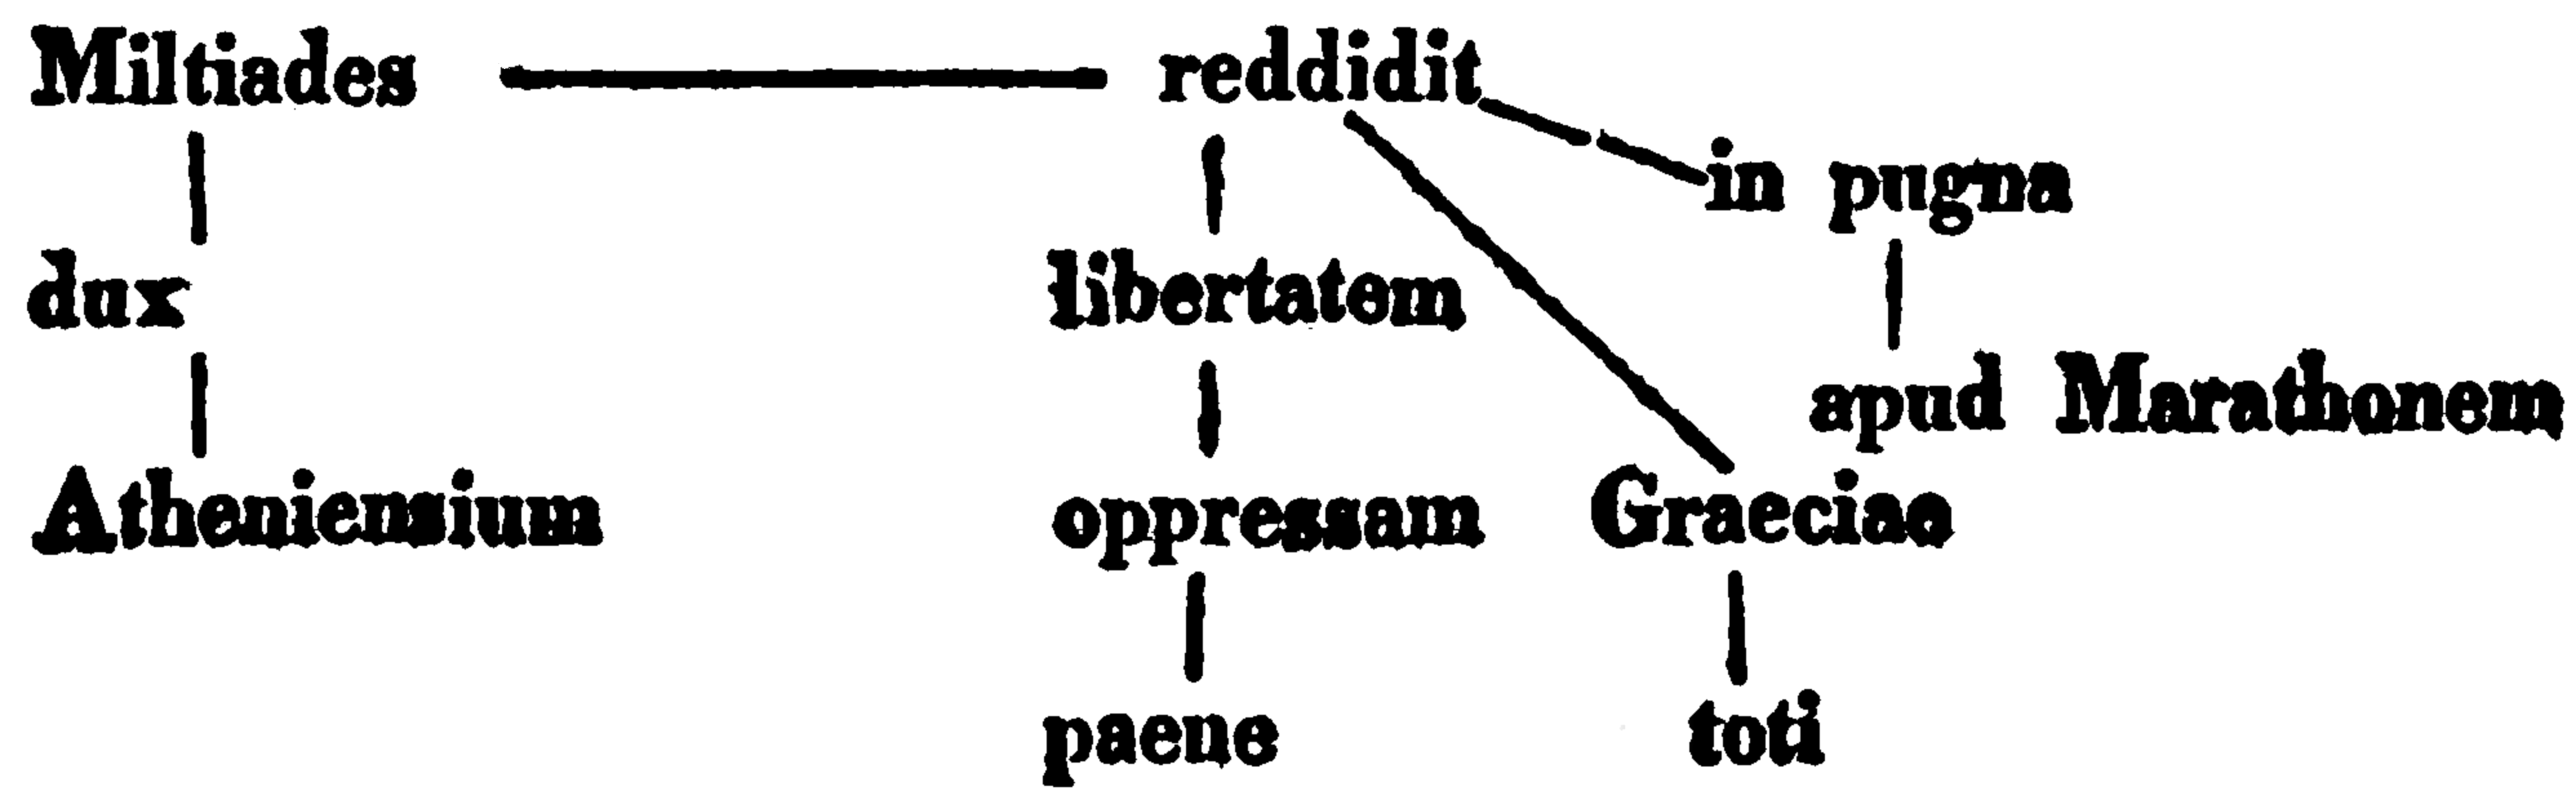
\includegraphics[width=.75\textwidth]{figures/Billroth1832.png}
    \caption{\label{fig:}Diagramme de \citet[102]{Billroth1832}}
    \textit{Miltiades, dux Atheniensium, toti Graeciae libertatem paene oppressam in pugna apud Marathonem reddidit.}
    ‘Miltiades, le chef des Athéniens, rendit à toute la Grèce la liberté dont elle avait été gravement privée en livrant bataille à Marathon.’
    \end{figure}

    Stephen W. Clark est le premier grammairien à réellement exploiter des diagrammes dépendentiels dans sa grammaire de l’anglais de \citeyear{Clark1847} intitulé \textit{The science of the English grammar: A practical grammar in which words, phrases, and sentences are classified to their offices, and their relation to each other, illustrated by a complete system of diagrams} ‘La science de la grammaire anglaise : une grammaire pratique dans laquelle les mots, les syntagmes et les phrases sont classées selon leurs fonctions et leurs relations les uns aux autres par un système complet de diagrammes’. Dans les représentations de Clark, les connexions ne sont pas représentées en tant que telles : un mot qui en «~qualifie~» un autre (pour reprendre les termes de Clark) est placé dans une bulle sous la bulle de son gouverneur. Les prépositions comme \textit{by} ‘par’ ou \textit{of} ‘de’ dans la figure ci-dessous reçoivent une forme particulière indiquant qu’elles servent à «~connecter~» deux mots. Le sujet, le verbe et l’objet direct sont placés au même niveau, comme ici \textit{ressources} and \textit{are developed}. Les groupes prépositionnels sont entourés par des bulles en pointillés.

    \begin{figure}[H]
    \caption{\label{fig:}Diagramme de \citet[17]{Clark1847}}
    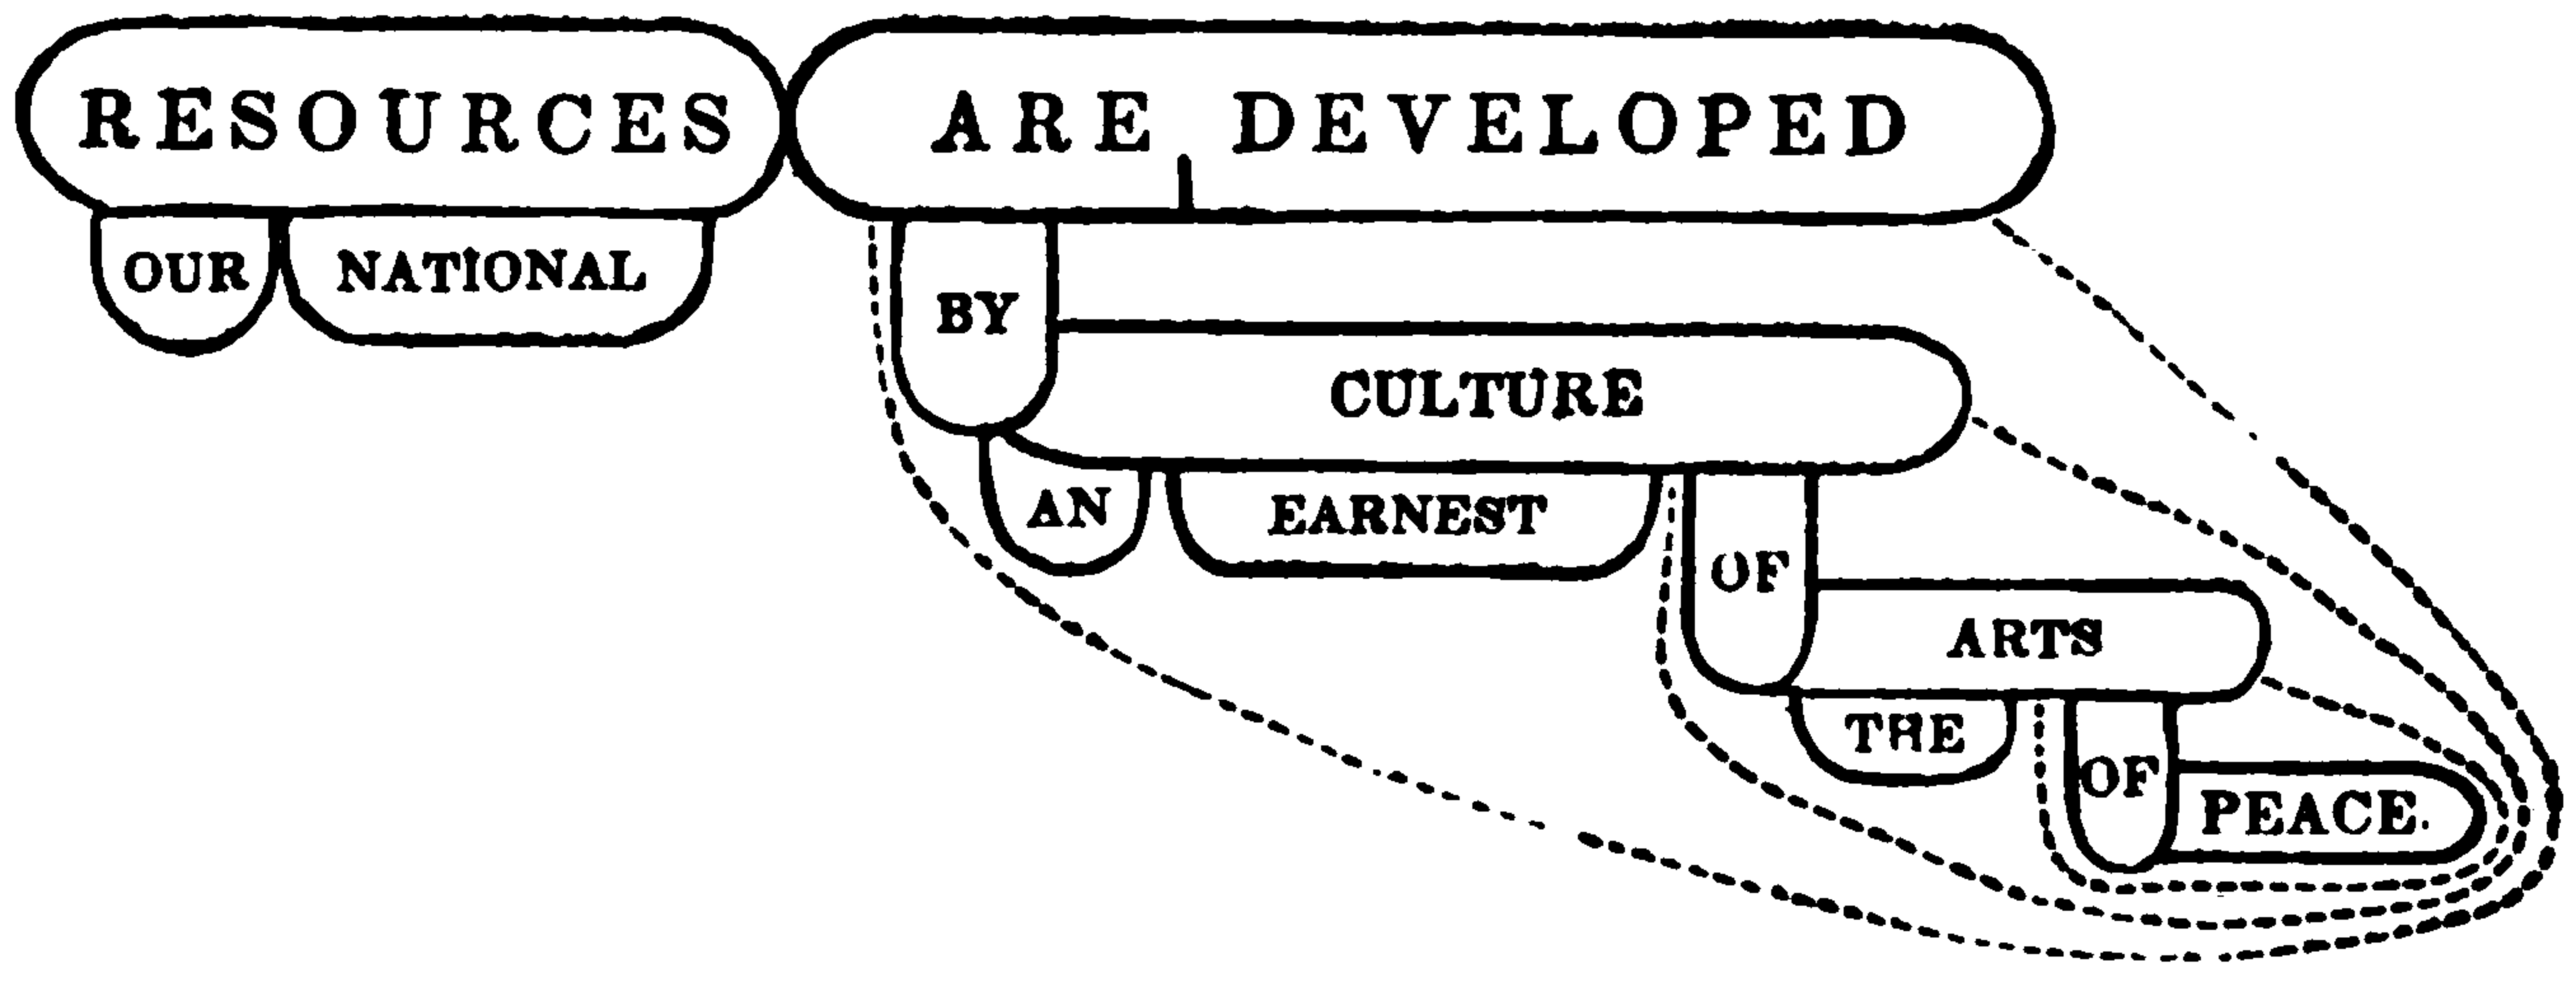
\includegraphics[width=.75\textwidth]{figures/Clark1847.png}\medskip\\
    \textit{Our national resources are developed by an earnest culture of the arts of peace.}
    ‘Nos ressources nationales sont développées grâce à une sérieuse culture des arts de la paix.’
    \end{figure}

    Les analyses de Clark sont d’une grande cohérence et ses représentations de la coordination ou de l’extraction, sur lesquelles nous reviendrons dans les chapitres \ref{sec:5.3} et \ref{sec:5.4}, sont remarquables. Il leur manque juste le développement théorique que proposera plus tard Tesnière.

    Ce ne sont pas les diagrammes de Clark qui sont passés à la postérité, mais ceux de ses suiveurs, \textbf{Alonzo Reed} and \textbf{Brainerd Kellogg}. Leurs diagrammes, proposés pour la première fois en \citeyear{ReedKellogg1877} et toujours utilisés aujourd’hui par certains enseignants d’anglais, sont équivalents à ceux de Clark, mais utilisent des conventions différentes : les mots ne sont plus placés dans des bulles, mais au-dessus de segments de traits. Les verbes et les noms reçoivent des segments horizontaux, comme \textit{pleased} ‘enchanté’ ou \textit{news} ‘nouvelles’ dans le diagramme qui suit, tandis que les autres mots, comme la préposition \textit{with} ‘avec’ ou l’adjectif ‘good’, reçoivent des segments en diagonal. Comme chez Clark, le sujet le verbe et l’objet sont au même niveau. Les connections apparaissent de manière plus explicite à la jointure de deux segments. La connexion entre le sujet et le verbe (\textit{girls – are pleased}) est symbolisée par un trait vertical et celle entre l’auxiliaire et le participe (\textit{are – pleased}) par un trait oblique.

    \begin{figure}[H]
    %%[Warning: Draw object ignored]
    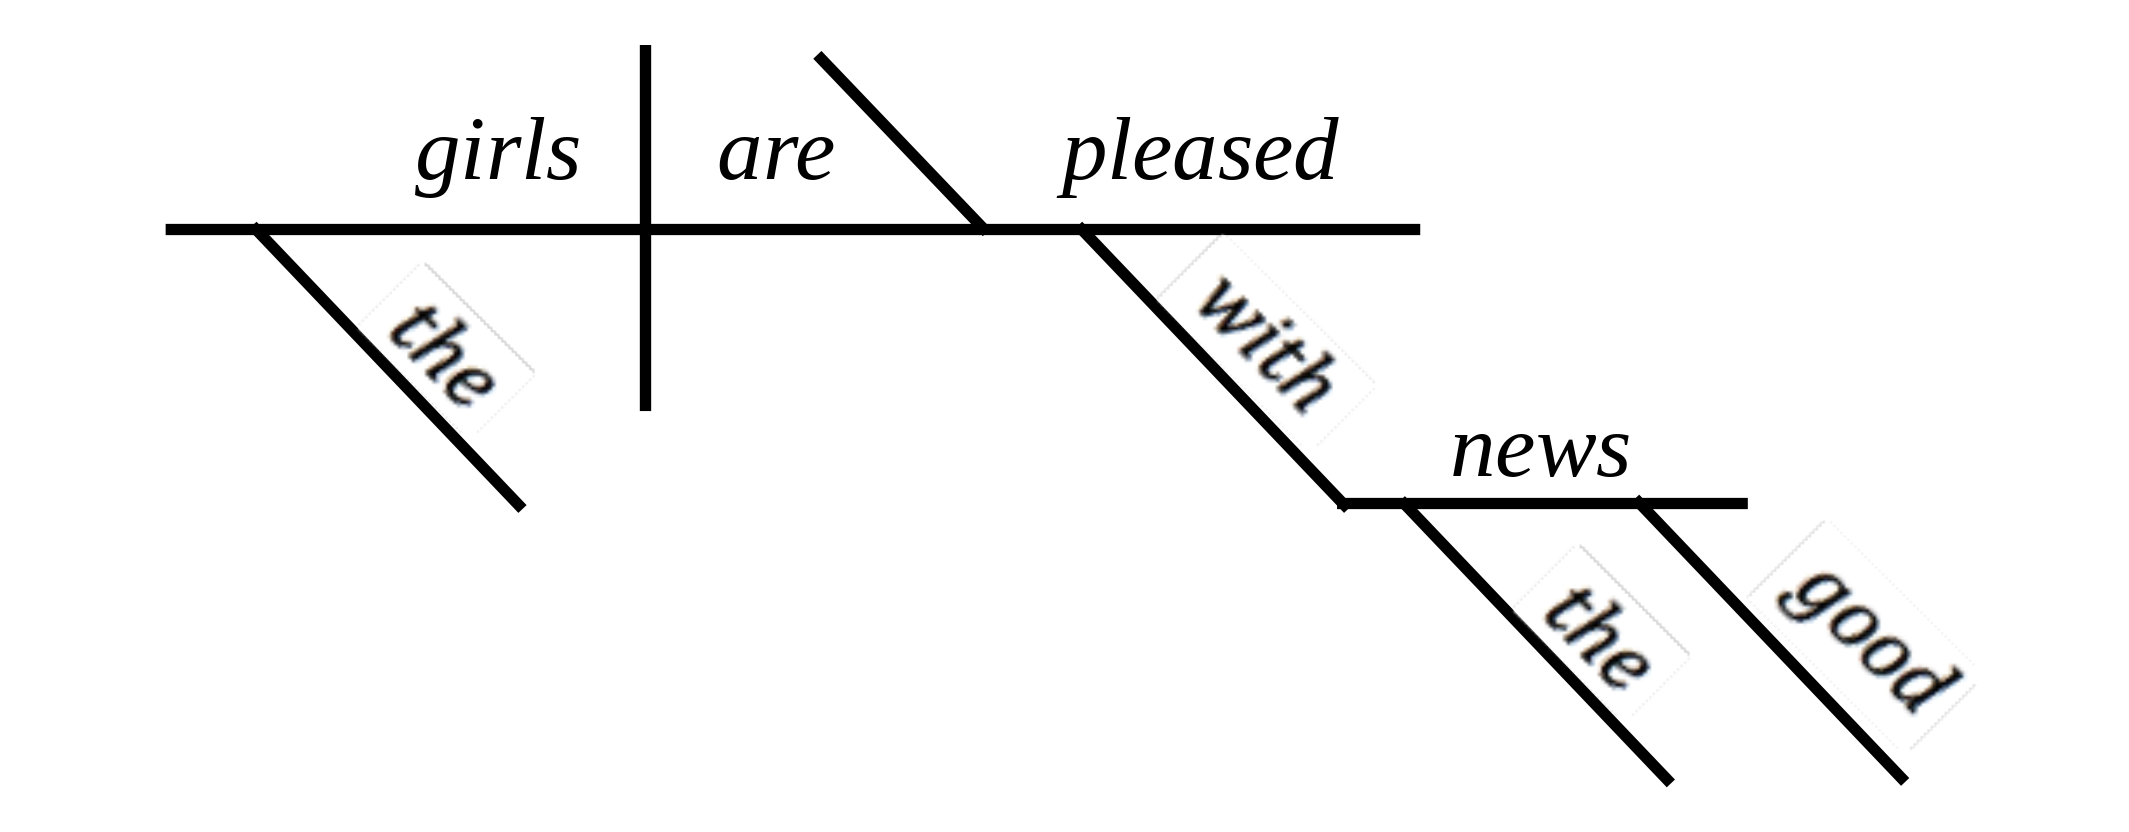
\includegraphics[width=7cm]{figures/ReedKellog}\medskip\\
    \raggedright\textit{The girls are pleased with the good news.}\\
    ‘Les filles sont enchantées par la bonne nouvelle.’\\
    \caption{Diagramme de \citet{ReedKellogg1877}}
    \end{figure}

    On peut traduire cette structure dans les conventions utilisées ici, en réifiant les connexions et en mettant en évidence le fait que certaines connexions ne sont pas hiérarchisées :

    \begin{figure}[H]
    \caption{Interprétation du diagramme de Reed \& Kellogg}
% %     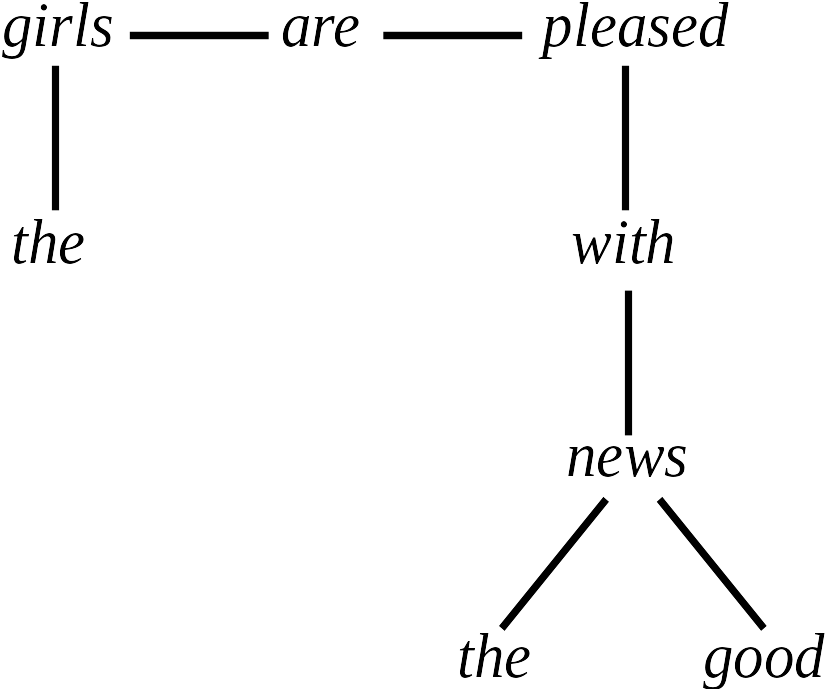
\includegraphics[width=7cm]{figures/ReedKellogTree}    
    \begin{forest} for tree={font=\itshape\strut}
    [,phantom,s sep=20pt
    [girls
      [the]
    ]
      [are,grow=east,tikz={\draw()--(!s);}
        [pleased
          [with
            [news
              [the] [good]
            ]
          ]
        ]
      ]   
    ]
    \end{forest}
    \end{figure}

    En \citeyear{kern1883zur}, dans un livre sur la grammaire allemande (\textit{Zur Methodik des deutschen Unterrichts} ‘Sur la méthodologie de l’enseignement de l’allemand’), \textbf{Franz Kern} propose de véritables arbres de dépendance. Voici ce qu’il écrit : «~Le mot déterminant dépend de celui qu’il détermine ou, en d’autres termes, est régi par lui. On désigne (graphiquement, par un schéma) la dépendance d’un mot d’un autre par un trait partant du mot régissant vers le bas et allant vers le mot régi~(ou dépendant) [figure de gauche] ou encore sans mot par de simples relations grammaticales [figure de droite].~» Ce texte est accompagné des deux figures suivantes pour la phrase \textit{Eine alte Kirche wurde ausgebessert} ‘Une vielle église a été réparée’. Dans la figure de gauche figurent les mots de la phrase, le complexe verbal n’étant pas décomposé. Dans la figure de droite, l’article (appelé \textit{Adj. (Zeiger)} ‘adjectif (pointeur)’) et l’adjectif qualificatif (\textit{Adjektiv}) dépendent du mot sujet (\textit{Subjektswort}) qui dépend du verbe fini (\textit{Finites Verbum}).

    \begin{figure}[H]
      \caption{Arbres de dépendance de \citet[10]{kern1883zur}}
    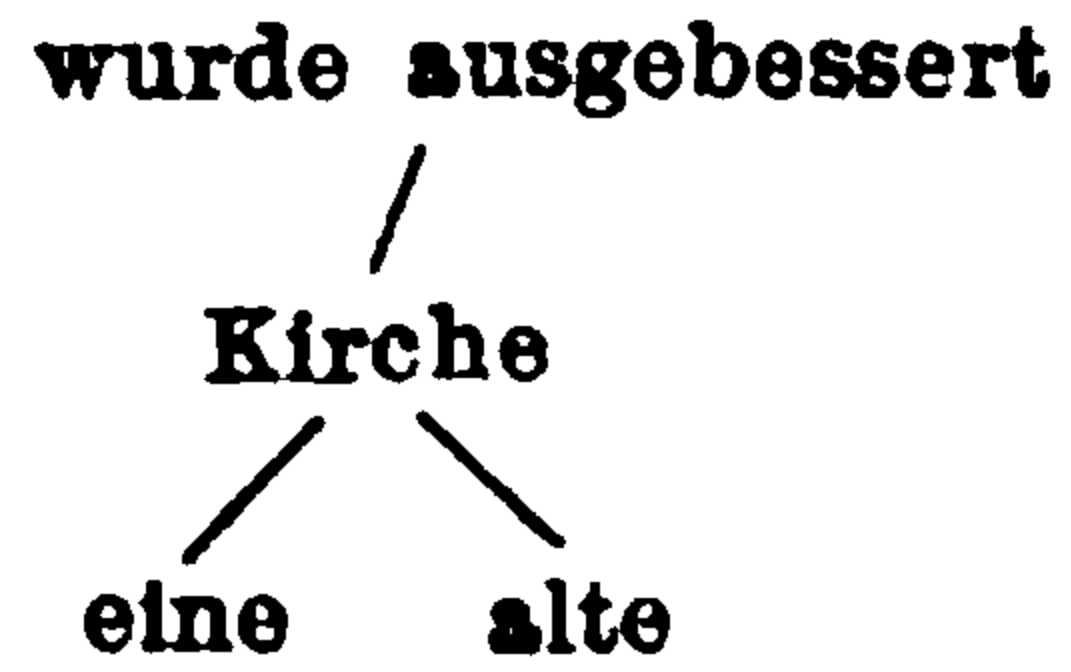
\includegraphics[height=2cm]{figures/Kern1883-1.png}
    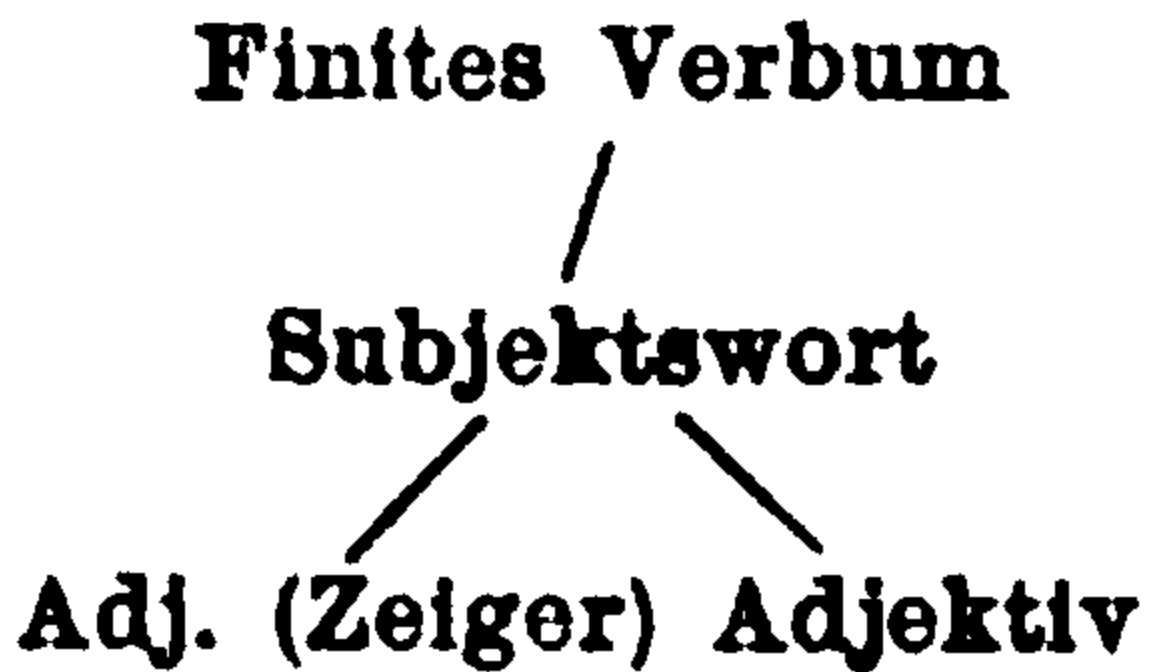
\includegraphics[height=2cm]{figures/Kern1883-2.png}\medskip\\
    \raggedright 
    \textit{Eine alte Kirche wurde ausgebessert.}\\
    ‘Une ancienne église a été reconstruite.’
    \end{figure}

    La notion de \textit{valence} a été introduite par le sémioticien anglais Charles S. Peirce dans un article de \citeyear{peirce1897logic}. Peirce compare la possibilité qu’a le verbe \textit{give} ‘donner’ de se combiner avec trois éléments (\textit{John gives John to John}) avec la possibilité qu’à l’atome d’azote N de se combiner avec trois atomes d’hydrogène H pour donner une molécule d’ammoniac NH\textsubscript{3}. Cette métaphore de la connexion entre mots par la connexion entre atomes est accompagnée de la figure suivante :

    \begin{figure}[H]
    \caption{Schéma valenciel de \citet{Peirce1897}}
    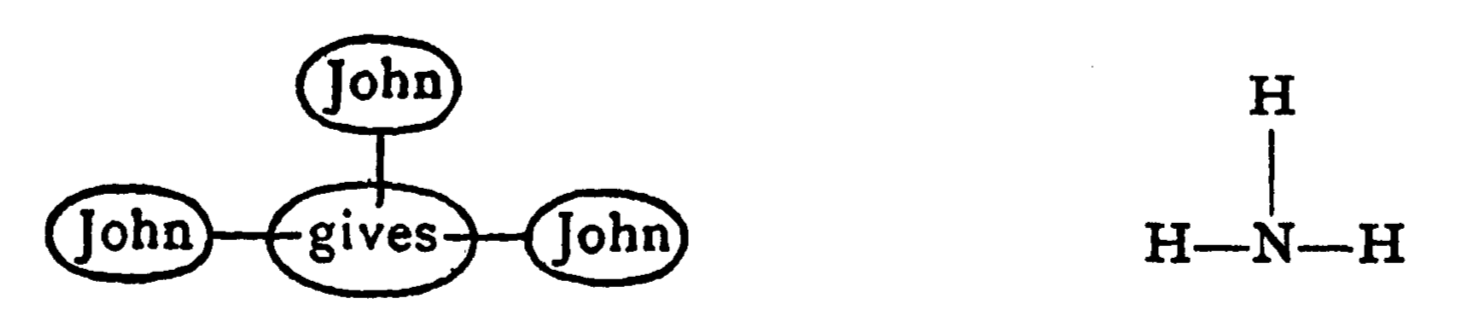
\includegraphics[width=\textwidth]{figures/vol1syntaxe2-img016.png}
    \end{figure}

    Peirce remarque que contrairement aux connections chimiques les connections entre mots (il s’agit plutôt de connexions sémantiques que syntaxiques) sont asymétriques, ce que semble confirmer son diagramme, où les connexions partent du mot \textit{gives} mais s’arrêtent à la bulle de \textit{John}. (Voir la \sectref{sec:3.3.10} sur \textit{Distribution et valence} pour la suite de la discussion.)

    C’est à Lucien Tesnière qu’on attribue les bases théoriques de la syntaxe de dépendance, exposées brièvement dans son article de \citeyear{tesniere1934comment}, \textit{Comment construire une syntaxe}, puis en détail dans son ouvrage posthume de \citeyear{tesniere1959elements}, \textit{Éléments de syntaxe structurale}. On notera, dans l’analyse suivante de 1934, que Tesnière considère la préposition comme dépendant du nom qu’elle introduit. (Le diagramme contient par ailleurs une erreur, qui n’est pas dans le manuscrit de Tesnière : le lien entre \textit{apporte} et \textit{vigueur} a été erronément attribué à \textit{elle}.)

    \begin{figure}[H]
    \caption{Diagramme (tronqué) de \citet{tesniere1934comment}}
    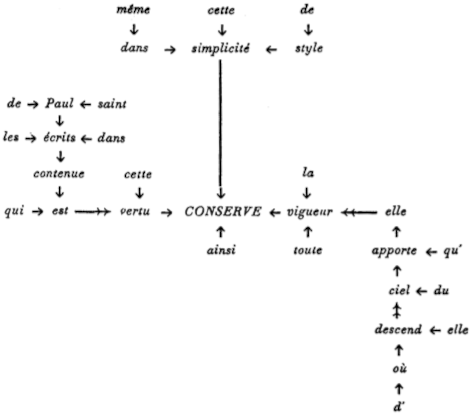
\includegraphics[width=\textwidth]{figures/vol1syntaxe2-img017.png}\medskip\\
    \textit{Ainsi cette vertu céleste, qui est contenue dans les écrits de saint Paul, même dans cette simplicité de style, conserve toute la vigueur qu’elle apporte du ciel d’où elle descend.} (Bossuet)
    \end{figure}

    Si cette analyse contient déjà des symboles spéciaux (comme les flèches à double pointe \textrm{$\twoheadrightarrow $} pour les relatives), ce n’est que plus tard que Tesnière introduira les symboles en T pour la translation. Les structures de l’ouvrage de 1959 ne sont plus totalement hiérarchique comme le montre notre interprétation polygraphique ci-dessous de la représentation proposée par Tesnière pour \textit{Écrivez dans le livre de votre ami} !.

    \begin{figure}[H]
    \caption{Interprétation polygraphique d'un stemma}
    \begin{subfigure}[b]{.5\textwidth}\centering
% %     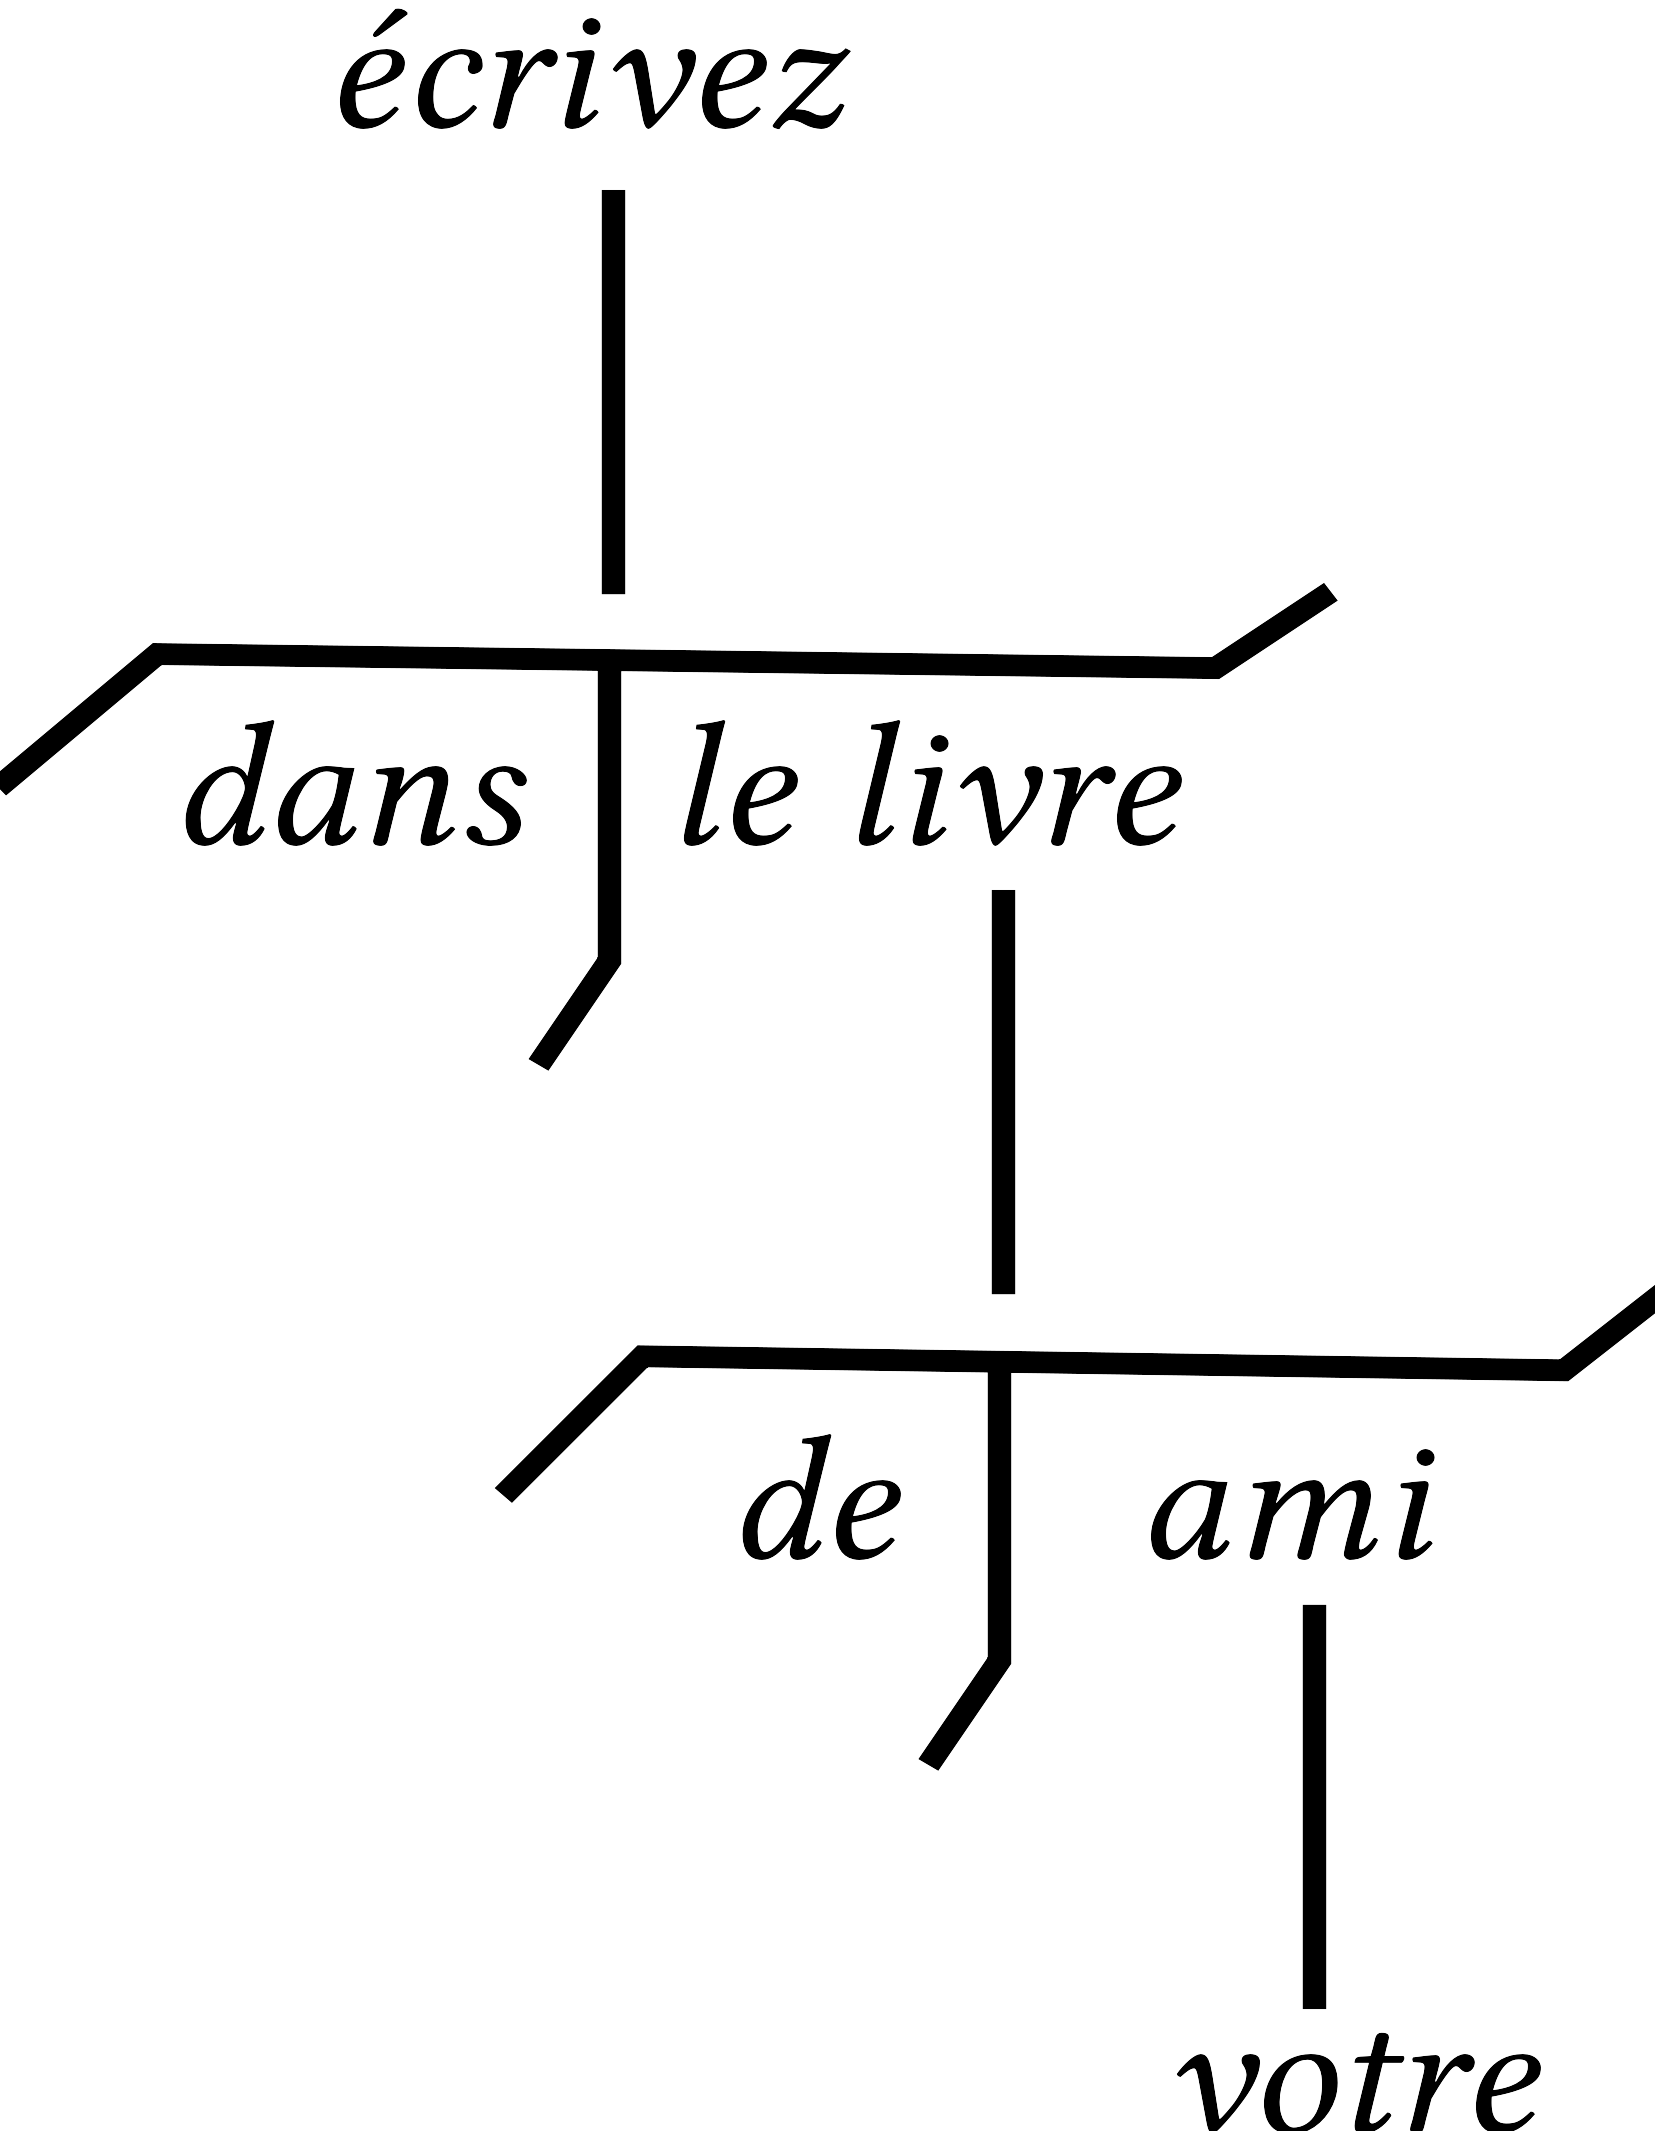
\includegraphics[width=4cm]{figures/StemmadeTesniere}
         \begin{tikzpicture}
           \node (dans) at (.5,3) {\textit{dans}};
           \node (écrivez) at (1,4.3) {\textit{écrivez}};
           \node (de) at (1.4,1.5) {\textit{de}};
           \node (le livre) at (1.7,3) {\textit{le livre}};
           \node (ami) at (2.2,1.5) {\textit{ami}};
           \node (votre) at (2.2,0.5) {\textit{votre}};
         
           \draw[thick] (dans.north west) -- (le livre.north east);
           \draw[thick] (de.north west) -- (ami.north east);
           \draw[thick] (dans.north east) -- (dans.south east);
           \draw[thick] (de.north east) -- (de.south east);
         
           \draw[thick] (dans.north west) -- +(-2mm, -2mm);
           \draw[thick] (le livre.north east) -- +(2mm, 2mm);
           \draw[thick] (de.north west) -- +(-2mm, -2mm);
           \draw[thick] (ami.north east) -- +(2mm, 2mm);
         
         
           \draw[thick] (de.south east) -- +(-2mm, -2mm);
         
           \draw[thick,shorten >=2mm] (écrivez) -- (1,3);
           \draw[thick,shorten >=4mm] (le livre) -- (1.7,1.5);
           \draw[thick] (ami) -- (votre);
         \end{tikzpicture}
    \caption{Stemma de \citet{tesniere1959elements}}
    \end{subfigure}%
    \begin{subfigure}[b]{.5\textwidth}\centering
% %     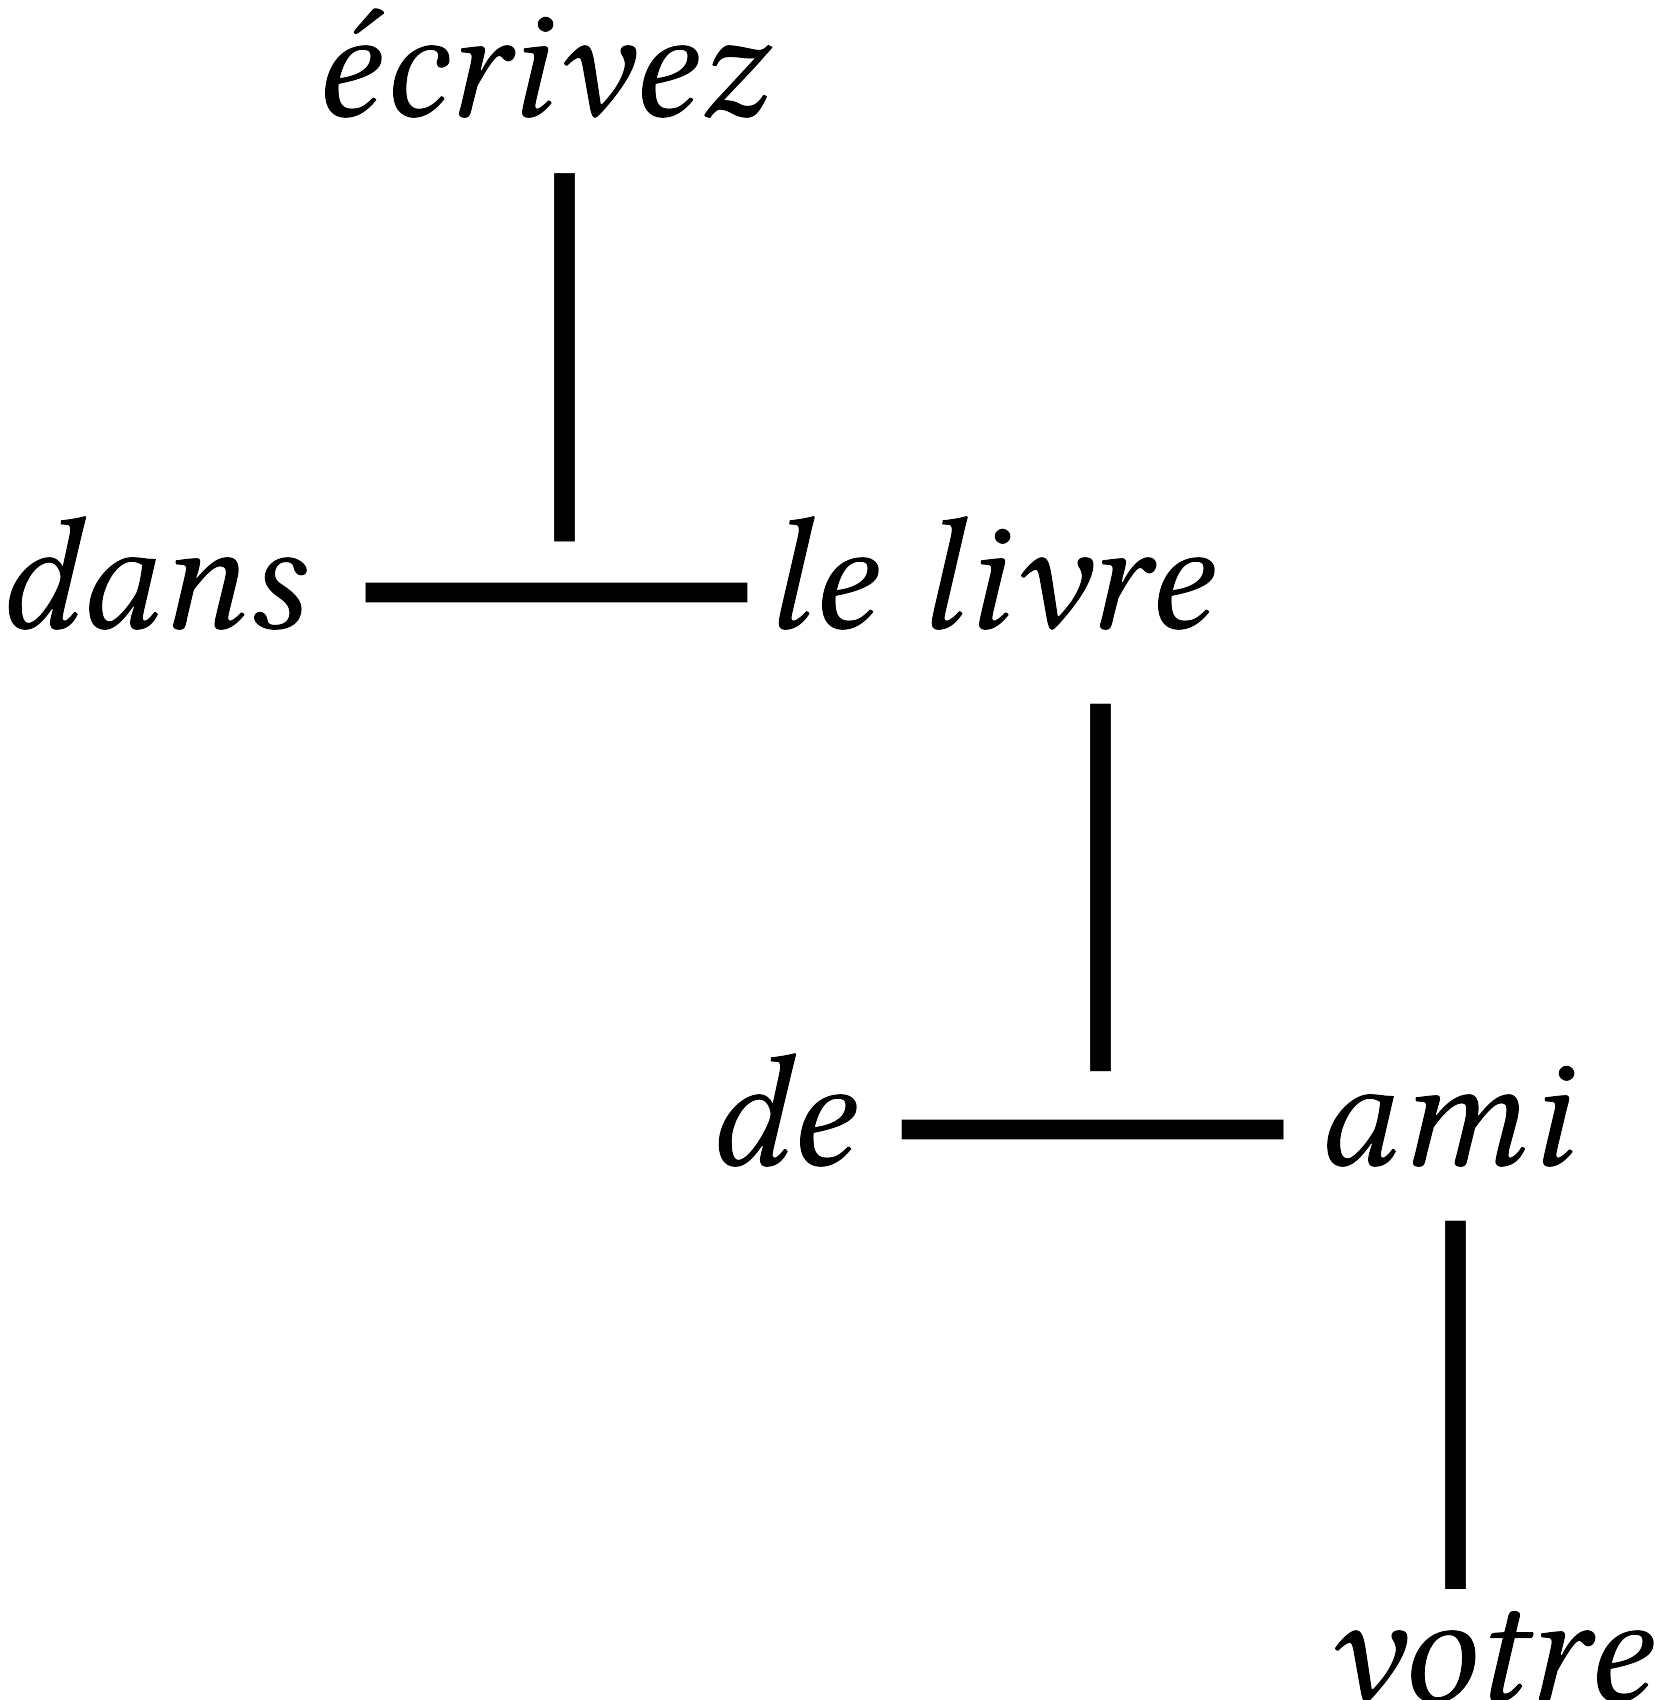
\includegraphics[width=4cm]{figures/Stemma}
        \begin{tikzpicture}
          \node (dans) at (.5,3) {\textit{dans}};
          \node (écrivez) at (1,4) {\textit{écrivez}};
          \node (de) at (1.5,2) {\textit{de}};
          \node (le livre) at (2,3) {\textit{le livre}};
          \node (ami) at (2.5,2) {\textit{ami}};
          \node (votre) at (2.5,1) {\textit{votre}};
        
          \draw[thick] (dans) -- (le livre);
          \draw[thick] (de) -- (ami);
          \draw[thick,shorten >=2mm] (écrivez) -- (1,3);
          \draw[thick,shorten >=2mm] (le livre) -- (2,2);
          \draw[thick] (ami) -- (votre);
        \end{tikzpicture}
    \caption{Interprétation polygraphique}
    \end{subfigure}
    \end{figure}
\todo[inline]{figure (a): the T shape of "de ami" is ok. The T shpe of "dans le livre must be identical, including the small space on top.}
\todo[inline]{figure (b): the line between "dans" and "le livre" must be longer and the vertical line must be centered on the horizontal line. Idem for "de" and "ami". .}
}

\section{Arbre et représentation planaire}\label{sec:3.3.6}

Il est essentiel de rappeler que la \textbf{représentation par un arbre (de} \textbf{dépendance)} sert uniquement à encoder une \textbf{structure hiérarchique} liant des nœuds entre eux par des relations père-fils. Dès qu’un arbre est représenté sur une feuille plane, les nœuds frères (c’est-à-dire ayant le même père) doivent être placés les uns à côté des autres et apparaissent donc comme ordonnés. Cet ordre sur les nœuds frères, imposé par la \textbf{représentation planaire}, est souvent utilisé pour encoder d'autres informations comme la saillance syntaxique (chez Tesnière par exemple) (voir \chapfuturef{15}) ou la saillance communicative (chez les Pragois) (voir l'\encadref{3.5.24} \textit{Ordre communicativement dirigé}). Un arbre avec un ordre sur les nœuds frères est une structure plus riche qu’un simple arbre. Les arbres que nous considérons dans ce chapitre sont des \textbf{arbres non ordonnés}. Il faut se les imaginer dans l’espace, libérés de la feuille, comme des \textbf{mobiles} suspendus dans l’air et dont les nœuds peuvent tourner librement autour de leur gouverneur.

Pour en faciliter la lecture, nous placerons généralement les nœuds de nos arbres dans l’ordre qu’ils occupent dans la phrase, mais cet ordre n’a aucune pertinence lorsque l’arbre est considéré en tant que tel et nos lecteurs devront essayer d’en faire abstraction. Libérez les arbres de la feuille ! Faites-les tourner dans votre tête !

Nous allons maintenant voir comment définir l’arbre de dépendance. Pour cela nous allons introduire différents critères permettant d’identifier la tête d’une unité syntaxique.

\section{Critère d’effacement simple et critère prosodique}\label{sec:3.3.7}

Une première définition possible d’une structure de dépendance se base sur la structure de connexion. Lorsqu’on possède déjà une structure de connexion, on peut la hiérarchiser (au moins partiellement) simplement en choisissant un nœud racine dans la structure. On peut alors orienter les connexions en partant de la racine. Tout se passe comme si on attrapait la structure par ce nœud et qu’on la suspendait.

Illustrons cela avec la phrase :

\ea \textit{Pierre veut inviter Marie demain.}\z

Si l’on a la structure de connexion de cette phrase (voir \chapref{sec:3.2}) et qu’on peut établir que \textit{veut} est la tête (voir \sectref{sec:3.3.8} suivante), on obtient immédiatement une structure de dépendance par le procédé que nous venons de décrire, comme le montre la figure \ref{fig:hierarchie}. La flèche blanche
\todo[inline]{The text must be finalized when the types of the arrows have been decided.}
indique le nœud par lequel on attrape la structure pour la hiérarchiser. Ce nœud va gouverner les nœuds auxquels il est connecté, lesquels vont gouverner à leur tour les nœuds auxquels ils sont connectés et ainsi de suite.

\begin{figure}
\vskip\baselineskip
\caption{Hiérarchisation d'une structure de connexion\label{fig:hierarchie}}
\begin{tabular}{@{}>{\centering}m{5cm} m{2em} >{\centering\arraybackslash}m{5cm} @{}}
  \begin{tikzpicture}[every node/.style={ConcSet}]
    \node at (0,0)   (Pierre) {Pierre};
    \node at (1,-1.5)  (veut) {veut};
    \node at (2,0)   (inviter) {inviter};
    \node at (3,1.5)   (Marie) {Marie};
    \node at (3,-1.5)  (demain) {demain};
    \draw (Pierre) -- (veut) -- (inviter) -- (Marie);
    \draw (inviter) -- (demain);
    \draw [ConversionArrow] (veut) ++(-1,-1) -- (veut);
  \end{tikzpicture} 
  & \tikz \draw[ConversionArrow] (0,0) -- (1,0); 
  & \begin{tikzpicture}[every node/.style={ConcSet},
                        edge from parent/.style={draw,-{Triangle[]}},
                        sibling distance=2cm
                        ]
  \node (root) {veut}
    child { node {Pierre} }
    child { node {inviter} 
            child { node {Marie} }
            child { node {demain } }
    };
  \draw [ConversionArrow,overlay] (root) ++(0,1.33) -- (root);
  \end{tikzpicture}\\
  Structure de connexion & & Arbre de dépendance
\end{tabular}
\end{figure}
\todo[inline]{The arrow between the two subfigures indicates a conversion: transformation of the left figure implies the right figure. A big \textbackslash Longrightarrow would be ok.}
\todo[inline]{The arrow in the two subfigures pointing on "veut" is a pointer. I would like a fat arrow, white or black. The same pointers appear in figures in chapter 3.}

Si la structure de connexion n’a que des connexions élémentaires (voir l’\encadref{fig:3.2.23} \textit{Graphe à bulles et polygraphe}) et pas de cycles, on obtient un arbre de dépendance, comme dans l’exemple précédent.

Baser ainsi la dépendance sur la connexion, revient à donner une importance première aux propriétés définitoires des unités syntaxiques, l’\textstyleTermes{autonomisabilité illocutoire} et l’\textstyleTermes{autonomisabilité prosodique} (voir la \sectref{sec:3.2.11} \textit{Unité syntaxique autonomisable}). Traduit pour le repérage de la tête d’une unité, ces deux critères deviennent le critère d’effacement simple et le critère prosodique.

L’autonomisabilité illocutoire donne le critère suivant.

\Definition{Critère d’effacement simple}
{\textstyleTermes{Critère d’effacement simple} : si \textbf{l’unité} \textbf{AB est gouvernée par X} et que \textbf{B peut être effacé}, mais pas A, alors \textbf{A est la tête de AB} et B dépend de A.}

Dire que B peut être effacé et pas A lorsque AB est gouverné par X revient à dire que XA peut former une unité (illocutoirement) autonome, mais pas XB et donc que X est connecté à A. Comme X est le gouverneur de AB, on en déduit que A est la tête de AB.

On peut illustrer l'application du critère d'effacement simple sur le syntagme \textit{demain matin} dans la phrase \textit{Pierre part demain matin.}
On a donc X = \textit{part,} A = \textit{demain} et B = \textit{matin}. Une fois établi que X est la tête de la phrase et gouverne donc AB, alors on en déduit que B dépend de A, car B est effaçable (\textit{Pierre part demain}), mais pas A (*\textit{Pierre part matin}).

\begin{figure}
\begin{tikzpicture}[baseline]
\node at (0,0) (X) {X};
\node at (1.5,0) (A) {A};
\node at (2.5,0) (B) {B};

\node [draw,ellipse,inner sep=0pt,fit=(A) (B)] (AB) {};
\draw (A) -- (B);
\draw [-{Triangle[]}] (X) -- (AB);

\draw[ConversionArrow] (3.5,0) -- (4.5,0);
\node at (5,0) (X) {X};
\node at (6,0) (A) {A};
\node at (7,0) (B) {B};

\draw [-{Triangle[]}] (X) -- (A);
\draw [-{Triangle[]}] (A) -- (B);
\end{tikzpicture}
\caption{\label{fig:}Application du critère d’effacement simple}
\end{figure}
\todo[inline]{Same \textbackslash Longrightarrow would be ok.}

Attention : la présence d’un gouverneur est essentielle dans la formulation du  critère d’effacement simple. On trouve souvent la \textbf{mauvaise formulation} suivante : le dépendant d’une connexion est l’élément qui peut le plus facilement être effacé. Cette propriété n’est valable qu’en présence d’un gouverneur. Si AB est un énoncé autonome ou plus généralement si AB n’est pas gouverné on peut très bien effacer la tête de AB. Par exemple, dans \textit{Zoé chantait} (A = \textit{chantait}, B = \textit{Zoé}), on peut effacer A et pas B (\textit{Zoé} peut former un énoncé autonome, mais pas \textit{chantait}), alors que c’est A qui est la tête !

Passons maintenant à l’autonomisabilité prosodique, le deuxième critère qui nous a permis de définir la structure de connexion. L’autonomisabilité prosodique donne le critère suivant.

\Definition{\textstyleTermes{critère prosodique}}
{\textstyleTermes{critère prosodique~}: si X est le gouverneur de AB et si X \textbf{peut former une unité prosodique avec} A sans B (sans changer significativement le sens), alors A est \textbf{la tête de l’unité} AB.}

Le critère prosodique reste d'un utilisation marginale et nous n'en donnerons pas d'exemple d'application.

Les deux critères que nous venons de proposer sont insuffisants pour plusieurs raisons.

Premièrement, ils ne s’appliquent que dans le cas où l’on étudie une unité qui possède un gouverneur. Ils ne peuvent donc pas être utilisés pour déterminer la tête d’un énoncé. Ce point va être étudié dans la section suivante.

Deuxièmement, il est assez courant que deux éléments qui se combinent soient indissociables, à l’intérieur du mot bien sûr (\textit{chant-ons}), mais aussi en dehors, comme \textit{le} et \textit{chien} dans \textit{le chien dort}. Dans ce cas, le critère d’effacement simple ne s’applique pas, pas plus que le critère prosodique en général.

Troisièmement, le critère d’effacement simple est inopérant si B est un dépendant obligatoire de A. C’est le cas pour une combinaison comme \textit{à Marie}, où A = \textit{à} ne peut pas s’employer sans son complément B et ne peut donc jamais former une unité XA avec le gouverneur X de AB. C’est encore le cas pour les formes verbales finies de langues comme le français : en effet, pour \textit{Marie dormait}, il n’est pas possible de vérifier si A = \textit{dormait} peut former une unité avec un éventuel gouverneur X, puisque A ne s’emploie jamais sans un sujet B. Ceci a d’ailleurs amené Leonard Bloomfield (qui fut le premier, dans son ouvrage \textit{Langage} de \citeyear{bloomfield1933language}, à proposer des critères pour définir la tête) à considérer que ces constructions sont \textstyleTermes{exocentriques,} c’est-à-dire sans tête (voir la \encadref{fig:3.3.2} \textit{Historique des notions de dépendance et de tête}.)

Les limites du critère d’effacement simple et du critère prosodique nous amènent à introduire d’autres critères plus puissants. Dans les critères que nous venons de considérer, le gouverneur X de l’unité AB que l’on étudie est fixé. On regarde seulement ce qui se passe dans une phrase donnée, sans faire varier X, A ou B. Cela confère à ces critères une grande simplicité d’utilisation, mais c’est aussi une limite. L’analyse distributionnelle va nous permettre de donner une version plus riche et plus fiable du critère d’effacement : le \textstyleTermes{critère distributionnel avec effacement}, présenté dans la \sectref{sec:3.3.11} éponyme.

\section{Tête d’un énoncé}\label{sec:3.3.8}

Comme nous l’avons vu à la section précédente, nous avons des critères pour identifier la tête d’une unité dès qu’on connaît son gouverneur, mais ces critères ne peuvent pas s’appliquer pour caractériser la tête d’un énoncé. Or, tant qu’on n’a pas identifié celle-ci et qu’on n’a pas un premier gouverneur, on ne peut pas appliquer le critère d’effacement simple ou le critère prosodique.

L’identification de la tête d’un énoncé repose sur les propriétés de l’énoncé en tant que tel, à savoir le fait qu’il fait l’objet d’une énonciation dirigée vers un interlocuteur et qu’il possède donc une \textstyleTermes{fonction illocutoire}. Cette notion repose sur le constat que produire un énoncé est une véritable action de la part du locuteur (on parle d’\textstyleTermes{actes de langage}, à la suite des travaux de \citet{gardiner1932speech}, John \citet{austin1962how} et John \citet{searle1969speech}), qui attend généralement en retour une action du ou des destinataire(s) (voir également la contribution de \citet{bloomfield1933language} dans la \sectref{sec:1.1.4} \textit{Sens et intention communicative}).

Ceci nous amène à considérer quatre types d’énoncés : \textstyleTermes{assertion}, \textstyleTermes{question}, \textstyleTermes{injonction} et \textstyleTermes{exclamation}.

\begin{itemize}
\item assertion : \textit{«~Il pleut.~»~}; \textit{«~J’ai mal au ventre.~»~};
\item question : «~\textit{Comment faire ?~»~}; «~\textit{Est-ce un problème ?~»} ;
\item injonction : «~\textit{Laissez ça ici !~»} ;
\item exclamation : «~\textit{Aie !~»~}; «~\textit{Comme c’est sympa !~».}
\end{itemize}

Les assertions peuvent être acceptés ou refusées par le destinataire ; elles se caractérisent par le fait de pouvoir être falsifiées par «~\textit{C’est faux.}~» ou au contraire validées par «~\textit{C’est vrai.}~». Par exemple, si quelqu’un nous dit «~\textit{J’ai mal au ventre}.~», on peut lui répondre «~\textit{C’est faux.}~», mais s’il dit «~\textit{Aie} !~», ce n’est plus possible. De même, on ne peut répondre «~\textit{C’est faux.}~» a une question ou une injonction. Les questions attentent une réponse. Les injonctions attendent généralement un acte non verbal. Les exclamations attendent simplement d’être partagées par le destinataire éventuel.

La fonction illocutoire a souvent un marquage spécifique. Les éléments qui servent à marquer la fonction illocutoire seront appelés des \textstyleTermes{marqueurs illocutoires}. La fonction illocutoire de l'énoncé conditionne son contexte, caractérise le type d'action que va effectuer en retour l'interlocuteur : acquiescer, répondre, obéir, etc. En conséquence, on considère que l'élément de l'énoncé qui porte la fonction illocutoire est la tête de l'énoncé.

\Definition{\textstyleTermes{critère illocutoire}}
{\textstyleTermes{critère illocutoire}. Les \textbf{marqueurs illocutoires} sont \textbf{portés} par la \textbf{tête syntaxique de l’énoncé} et la caractérise.}

En français, le principal marqueur illocutoire est la prosodie (transcrit à l’écrit par des signes de ponctuation comme « ?~» ou « !~»). Mais pour les énoncés à tête verbale en français, il existe d’autres marques. Voyons sur un exemple :

\ea
\textit{{Pierre a dormi}.}
\z

Cet énoncé est une assertion. Comme toute assertion, on peut la nier en répondant «~\textit{C’est faux}~».~La négation de cet énoncé (c'est-à-dire un énoncé ayant pour sens ‘il est faux que Pierre a dormi’) peut s’exprimer en français par un double marquage \textit{ne…pas} qui semble bien identifier l’auxiliaire comme la tête :

\ea
\textit{{Pierre} \textbf{{n’a}  {pas}}  {dormi.}}
\z

On peut également faire varier la fonction illocutoire et transformer cet énoncé en une question ou une injonction :

\ea
  \ea \textit{Pierre \textbf{a-t-il} dormi ?}
  \ex \textit{\textbf{Ais}  dormi (quand  je reviens)!}
  \z
\z

Le français a pour cela des formes particulières : une question peut prendre la \textstyleTermes{forme} dite \textstyleTermes{interrogative}, qui se caractérise par la présence d’un \textstyleTermes{enclitique} (\textit{{}-t-il} dans notre exemple) ; une injonction peut s’exprimer par une forme verbale particulière : l’\textstyleTermes{impératif} (ici \textit{ais}, forme impérative du verbe \textsc{avoir}). C’est encore une fois l’auxiliaire qui est touché, ce qui confirme son statut de tête.

On peut par la même méthode identifier la tête d’une phrase complexe avec deux verbes finis. Cette tête est traditionnellement appelée le \textstyleTermes{verbe principal}. Considérons :
\ea
\textit{{Marie pense que Pierre dort}.}
\z
La forme interrogative est \textit{Marie pense-t-elle que Pierre dort} ? et pas *\textit{Marie pense que Pierre dort-il} ? On en déduit que \textit{pense} est la forme verbale principale et que \textit{dort} est une forme verbale subordonnée.

\Definition{\textstyleTermes{subordination}, \textstyleTermes{proposition subordonnée}}
{La \textstyleTermes{subordination} est simplement le terme traditionnel pour désigner la \textbf{dépendance d’une} \textbf{forme verbale} à un autre élément.  Une proposition dont le verbe est subordonné est appelée une \textstyleTermes{proposition subordonnée}.}

On appelle \textstyleTermes{proposition} une unité de taille maximale dont la \textbf{tête} est une \textbf{forme verbale}. Nous donnerons une définition plus précise de la proposition dans la \sectref{3.3.30} sur \textit{Dominance et projections maximales}.

L’identification de la subordination nous procure un nouveau test pour repérer la tête d’une proposition (voir \textbf{critère rectionnel} à la \sectref{sec:3.3.16} \textit{Tête interne et critère rectionnel}). En effet, certains verbes imposent un mode particulier à leur subordonné. Par exemple, si l’on subordonne au verbe \textsc{falloir} la proposition \textit{Pierre a dormi}, on obtient \textit{Il faut que Pierre} \textbf{\textit{ait}} \textit{dormi (quand je reviens).} Comme on le voit, encore une fois, c’est l’auxiliaire qui hérite ici de la marque de subordination, à savoir le \textstyleTermes{mode subjonctif} (\textit{ait} est une forme subjonctive de \textsc{avoir}), ce qui confirme son statut de tête syntaxique de la proposition.

On peut encore utiliser ces différents critères pour repérer que certains énoncés n’ont pas une tête verbale. Comparons les deux phrases suivantes :

\ea 
  \ea \textit{Heureusement, Pierre a dormi.}
  \ex \textit{Heureusement que Pierre a dormi.}
  \z
\z

On peut subordonner le premier énoncé, mais pas le deuxième :

\ea
  \ea[]{\textit{Je crois que, heureusement, Pierre a dormi.}}
  \ex[*]{\textit{Je crois qu’heureusement que Pierre a dormi.}}
  \z
\z

Comme il apparaît par ailleurs que le verbe \textsc{croire} peut subordonner n’importe quelle proposition à l’indicatif, on peut supposer que la phrase introduite par \textit{heureusement que} ne peut pas être subordonnée car le verbe n’en est pas la tête. On en déduit que \textit{heureusement} est la tête de la phrase et subordonne la proposition \textit{Pierre a dormi} (ce que confirme l’emploi de la conjonction de subordination \textit{que}).

Le même type de raisonnement permet d’identifier la tête d’une proposition dans n’importe quelle langue a priori (voir encadré ci-dessous).

\globe{Tête d’un énoncé dans une langue inconnue}{%\label{sec:3.3.9}
    Comme nous l’avons dit dans les sections précédentes, l’identification de la tête d’un énoncé est un préalable à la hiérarchisation de la structure.

    Nous allons considérer le cas de deux langues non apparentées, l'anglais et le coréen. Le cas du wolof sera présenté dans la \sectref{3.3.16} sur \textit{Tête interne et critère rectionnel}.
    
  Commençons par l’\textbf{anglais}, qui est une langue très proche du français, mais dont le fonctionnement est quand même assez différent. Considérons l’énoncé \textit{Peter has slept} ‘Pierre a (déjà) dormi’. Comme en français, la négation va sur l’auxiliaire sur lequel elle se cliticise :
    \ea
        \textit{{Peter} \textbf{{hasn’t}}  {slept.}} \\\glt ‘Pierre n’a pas dormi.’
    \z
    Quant à la question, elle est normalement formée par l’antéposition de l’auxiliaire :
    \ea
        \textit{\textbf{{Has}}  {Peter slept?}} \\\glt   ‘Pierre a-t-il dormi ?’
    \z
    On peut considérer que cette place particulière de l’auxiliaire le marque comme la tête. D’ailleurs, un verbe ordinaire ne peut recevoir directement la négation, ni être antéposé. Le passage à une forme interrogative ou négative nécessite l’introduction de l’auxiliaire \textsc{do} ‘faire’ :
    
    \ea
      \ea \textit{Peter slept.}  \\\glt  ‘Pierre a dormi.’
      \ex \textit{\textbf{{Did}}  {Peter sleep?}}  \\\glt  ‘Pierre a-t-il dormi ?’
      \ex \textit{{Peter} \textbf{{didn’t}}  {sleep.}} \\\glt ‘Pierre n’a pas dormi.’
      \z
    \z
    Comme on le voit, la forme passé \textit{slept} passe à la forme infinitive. L’auxiliaire lui-même hérite de la finitude (\textit{did} est la forme passé de \textsc{do}) et constitue donc la tête de la phrase quand il est présent. En l’absence d’auxiliaire, c’est la forme verbale simple qui est la tête, puisque c’est elle qui est affectée lorsque l’auxiliaire est introduit. On notera que l’auxiliaire, bien qu’il soit la tête de la phrase, peut dans certains cas se cliticiser sur le sujet (c’est-à-dire perdre la possibilité de recevoir un accent tonique et former un mot prosodique avec le dernier mot du sujet) :
    
    \ea
      \ea \textit{{Peter}\textbf{{’s}}  {sleeping}} =  \textit{{Peter} \textbf{{is}}  {sleeping}} \\\glt ‘Pierre est en train de dormir’, lit. Pierre est dormant.
      \ex \textit{{Peter}\textbf{{’s}}  {eaten}}   =   \textit{{Peter} \textbf{{has}}  {eaten}}  \\\glt ‘Pierre a (déjà) mangé’
        \z
    \z
   
   En \textbf{coréen}, le verbe principal d’un énoncé est caractérisé par un marqueur de politesse qu’il est le seul à pouvoir porter. Cette particule s’ajoute optionnellement sur le verbe principal, mais jamais sur un verbe subordonné. Le coréen utilise essentiellement des constructions à verbe support (voir \encadref{2.3.9} sur \textit{Verbes supports et unités grammaticale}s) avec le verbe \textsc{hada} ‘faire’. Dans la phrase suivante, le sens ‘aimer’ est ainsi lexicalisé par le nom \textsc{sarang} ‘amour’ et le sens ‘croire’ par le nom \textsc{saenggak} ‘pensée’, tous deux «~verbalisés~» par le verbe \textsc{hada}. La deuxième occurrence de \textsc{hada} peut porter le morphème de politesse \textit{yo}, mais pas la première. (Nous reviendrons sur les marqueurs illocutoires du coréen dans l’encadré \textit{Des prédicatifs uniquement locutifs assertifs} du \chapfuturef{17}.)

    \ea
    \ea[]{
    \gll  철수가 나를 사랑한다고 생각해(-\textbf{요})\\
    Ch’ŏlsu-ga na-rŭl sarang-ha-ndago saenggak-hae(-\textbf{yo})\\
    Ch’ŏlsu-\textsc{nom}   moi-\textsc{acc}  amour-faire-\textsc{pres.inf}  pensée-faire(-\textsc{politesse)}\\
    \glt   ‘Je crois que Cholsu m’aime’}
    \ex[*]{
    \gll   철수가 나를 사랑해-\textbf{요}다고 생각해(-\textbf{요})\\
    Ch’ŏlsu-ga            na-rŭl            sarang-hae-\textbf{yo}-dago  saenggak-hae(-\textbf{yo})\\
    Ch’ŏlsu-\textsc{nom}  moi-\textsc{acc}  amour-faire-\textsc{politesse}-\textsc{pres.inf}  pensée-faire(-\textsc{politesse)}\\}
    \z
    \z
}
\section{Distribution et valence}\label{sec:3.3.10}

En nous basant sur la structure de connexion et en déterminant la tête de la proposition grâce aux marqueurs illocutoires, nous avons vu que nous pouvions obtenir une structure de dépendance partielle. Nous allons voir que l’on peut raffiner cette structure en ajoutant des critères additionnels. Les premiers de ces critères sont les critères distributionnels que nous présenterons dans les sections suivantes. Nous devons avant cela introduire les notions de distribution (voir l'\encadref{fig:2.1.7} sur \textit{L’identification des unités de la langue}, où il a été question d’analyse distributionnelle) et valence (voir la \sectref{sec:3.3.5} \textit{Historique des représentations syntaxiques par des diagrammes en dépendance} pour un début de discussion).

\Definition{\textstyleTermes{distribution}}
{La \textstyleTermes{distribution} d’une unité est l’\textbf{ensemble des contextes} ou \textbf{environnements} où peut se trouver cette unité.}

Deux remarques essentielles sont à faire concernant la distribution.

Premièrement, nous faisons de l’analyse distributionnelle sur un objet structuré. Ici, ce qui nous intéresse, c’est la \textstyleTermes{distribution syntaxique} et non la distribution linéaire. Nous nous intéressons donc au contexte des unités au sein de la structure syntaxique, c’est-à-dire au \textstyleTermes{paradigme} des unités qui se combinent avec l’unité que nous étudions.

La notion de distribution est encore exprimable en termes de valence.

\Definition{\textstyleTermes{valence}}
{La \textstyleTermes{valence} d’une unité syntaxique est la \textbf{capacité} qu’à cette unité \textbf{à se combiner} avec d’autres unités syntaxiques. La valence est avant tout une \textbf{valence potentielle}, à contraster avec la \textbf{valence réalisée}, lorsque l’unité est utilisée dans un contexte donné.}

Cette métaphore de la valence est inspirée de la chimie et de la capacité qu’à un atome à \textbf{se combiner avec d’autres} \textbf{atomes pour former des molécules} (voir la contribution de \citet{Peirce1897} dans l’\encadref{fig:3.3.5} \textit{Historique des représentations syntaxiques par des diagrammes en dépendance}, ainsi que les formules utilisées par \citet{jespersen1937analytic}, évoquées dans l’\encadref{fig:3.3.2} \textit{Historique des notions de dépendance et de tête}). Mais alors que les connexions entre atomes sont symétriques (chaque atome fournit un électron de même nature), les connexions entre unités sont doublement asymétriques : \textbf{asymétrie syntaxique}, puisqu’elles lient un gouverneur à un dépendant, et \textbf{asymétrie sémantique}, puisqu’elle lient un prédicat à un argument.

L’asymétrie syntaxique nous amène à distinguer deux parties dans la valence.

\Definition{\textstyleTermes{valence supérieure}}
{La \textstyleTermes{valence supérieure} d’une unité syntaxique U est la \textbf{position syntaxique} occupée par le \textbf{gouverneur} de U, cette position étant elle-même caractérisée par le \textbf{paradigme} des éléments qui peuvent l’occuper.}

\Definition{\textstyleTermes{valence inférieure}}
{A l’inverse, la \textstyleTermes{valence inférieure} d’une unité syntaxique est l’ensemble des positions syntaxiques qui \textbf{dépendent} potentiellement de cette unité.}

Les notions de valences supérieure et inférieure ont été introduites par Igor Mel’čuk, qui les nomment \textit{valence passive} et \textit{valence active}. Nous préférons garder ces termes pour parler de la partition de la valence selon le point de vue sémantique (voir \chapfuturefici{13}).

Deuxièmement, nous souhaitons utiliser l’analyse distributionnelle pour caractériser la tête d’une unité. Nous cherchons donc à repérer dans le contexte syntaxique d’une unité le contexte qui caractérise plus particulièrement la tête, c’est-à-dire la valence supérieure.

Illustrons ce dernier point par un exemple. Considérons l’énoncé \textit{Une très vieille dame habite ici} et l’unité syntaxique \textit{vieille dame} qu’il contient. Aucun des deux mots \textit{vieille} et \textit{dame} ne contrôlent à lui seul l’entièreté de la distribution de l’unité qu’ils forment ensemble, car \textit{vieille} est connecté à \textit{très} (\textit{très vieille}) et \textit{dame} est connecté à \textit{une} et \textit{habite} (\textit{une dame habite ici}). Bien sûr, une fois que l’on sait que \textit{habite} est la tête de la phrase, on en déduit que la tête de \textit{vielle dame} est \textit{dame}, puisque c’est le mot qui est connecté au gouverneur de cette unité syntaxique.

On ne dira jamais assez qu’on ne peut \textbf{déterminer la tête} d’une unité syntaxique U par la distribution qu’\textbf{une fois qu’on} \textbf{a déterminé la valence supérieure} de U, c’est-à-dire qu’on a déterminé qui parmi les éléments auxquels U est connectée gouverne U. Considérer la distribution sans avoir au préalable distingué valence inférieure et supérieure peut conduire à des erreurs méthodologiques. Il y a là un cercle vicieux dans lequel il faut éviter de rentrer, puisqu’on ne peut appliquer de critère distributionnel pour déterminer la tête d’une unité sans savoir où se trouve son gouverneur. Autrement dit, il s’agit d’un critère pour déterminer la hiérarchie qui ne peut s’appliquer qu'en connaissant déjà une partie de la hiérarchie.

Supposons que l’on veuille déterminer qui du nom ou du déterminant est la tête du groupe qu’ils forment ensemble (comme par exemple \textit{chat} et \textit{le} dans \textit{le chat dort}). Si l’on décrète que pouvoir être sujet d’un verbe fait partie de la valence supérieure du nom, le problème est biaisé, puisque, en un sens, on a déjà décidé que le nom est la tête du groupe qu’il forme avec le déterminant (on trouve cette erreur méthodologique dans l’ouvrage de référence d’Igor Mel’čuk de \citeyear{melcuk1988dependency}). Tout le problème ici est qu’on ne peut facilement déterminer la valence supérieure du nom seul, car, dans de nombreuses positions, il est indissociable d’un déterminant. (Voir la \sectref{sec:3.3.23} sur \textit{Nom ou déterminant comme tête} ?) Nous avons contourné ce problème en définissant au préalable la structure de connexion (\chapref{sec:3.2}), puis en hiérarchisant sommairement cette structure en déterminant la tête d’un énoncé (\sectref{sec:3.3.8}), ce qui nous permet de localiser la valence supérieure d’un certain nombre d’unités (mais pas des noms malheureusement !).

\section{Le critère distributionnel avec effacement}\label{sec:3.3.11}

Les critères distributionnels s’appliquent à une unité syntaxique U dont on connaît la \textbf{valence supérieure}, c’est-à-dire le \textbf{paradigme des gouverneurs possibles} (voir \sectref{sec:3.3.10}).
L'unité U est la combinaison libre de A et B (U = A ${\oplus}$ B) et on veut savoir qui de A ou B est la tête de U (et donc si A dépend de B ou l'inverse).

Nous allons voir deux critères distributionnels. Le premier, le critère distributionnel avec effacement suppose que A et B ne sont pas mutuellement indissociables pour être appliqué, c'est-à-dire que l'on peut utiliser A sans B ou B sans A. (Nous reviendrons sur les propriétés d'indissociabilité dans le \chapfuturef{15} , lorsque nous définirons la notion de \textit{mot}.)

\Definition{\textstyleTermes{critère distributionnel avec effacement}}
{\textstyleTermes{Critère distributionnel avec effacement}. Si U = A ${\oplus}$ B, que A est autonomisable (et donc B est effaçable) et que A à la même \textbf{valence supérieure} que U, alors A est un \textbf{tête} de U.
Inversement, si A n'a pas la même valence supérieure que U, alors B est une tête de U.}

\Definition{\textstyleTermes{tête distributionnelle}}
{Une sous-unité A de U qui est identifiée comme tête par un critère distributionnel est appelée une \textstyleTermes{tête distributionnelle} de U.}

Le critère distributionnel avec effacement généralise le critère d’effacement simple. Le critère d’effacement simple s’applique à une unité U à l’intérieur d’un énoncé donné, sans faire varier le gouverneur de U. Ici on considère la distribution de U, c’est-à-dire tous les gouverneurs potentiels de U.
\todo[inline]{Why there is no indentation in this section. Bug?}

Illustrons le critère par l’exemple de U = \textit{demain matin} avec A = \textit{demain} et B~= \textit{matin}. Ici A et B sont effaçables et on peut donc comparer la valence supérieure de A, B et U = A ${\oplus}$ B. Il est facile de voir que \textit{demain} et \textit{demain matin} ont la même valence supérieure : ils peuvent par exemple tous les deux être modifieur d'un verbe (\textit{Pierre part demain (matin).}) et tous les deux se comporter comme un groupe substantif ordinaire et être sujet d'un verbe (\textit{Demain (matin) me paraît le moment idéal.}) ou être complément d'un préposition (\textit{la réunion de demain (matin)}). Cette valence supérieure est différente de la valence supérieure de \textit{matin} qui ne peut apparaître dans aucun de ces contextes. On en déduit que \textit{demain} est la tête de U.

Le critère distributionnel avec effacement s’applique aussi dans des cas où le critère d’effacement simple ne s’applique pas. Reprenons l’exemple de U = \textit{à Marie}. Ici \textit{Marie} n’est pas effaçable, puisque \textit{à} n’est pas autonomisable. Par contre, \textit{à} est effaçable, on peut donc comparer les valences supérieures de \textit{Marie} et \textit{à Marie}. Ces deux unités ont des valences supérieures complètement différentes. Par exemple, \textit{Marie} peut être sujet (\textit{Marie dort}) ou complément d’objet (\textit{J’ai vu Marie}) et la commutation avec \textit{à Marie} est impossible (*\textit{A Marie dort} ; *\textit{J’ai vu à Marie}). On en déduit que \textit{à} est la tête de \textit{à Marie}.

Le même raisonnement est applicable à \textit{Marie dormait}. Ici encore, \textit{Marie} n’est pas effaçable, mais \textit{dormait} l’est. Comme \textit{Marie} et \textit{Marie dormait} n’ont absolument pas la même valence supérieure, on en déduit que \textit{dormait} est bien la tête de la proposition \textit{Marie dormait}.

\loupe{Tête effaçable}{%\label{sec:3.3.12}
    Il arrive quelquefois que le critère d’effacement simple et le critère distributionnel avec effacement se contredisent. On parle alors de \textstyleTermesapprofondissement{tête effaçable}. L’exemple le plus clair est celui de la conjonction de subordination \textit{that} en anglais. Voyons un exemple :
    \ea
        \textit{{Mary thinks that Peter slept.}}  ‘Mary pense que Pierre dormait.’
    \ex
        \textit{{Mary thinks Peter slept.}}    ‘Mary pense que Pierre dormait.’
    \z
    La conjonction \textit{that} est bien effaçable, ce qui pourrait conduire à considérer que \textit{thinks} est directement connecté à \textit{slept}. Mais en même temps on ne peut pas considérer que \textit{that} dépend de \textit{slept}, car \textit{that Peter slept} n’a pas la même valence supérieure que \textit{Peter slept} : si les deux peuvent dépendre de \textit{Mary thinks}, seul \textit{Peter slept} peut former un énoncé déclaratif ou bien se combiner avec une conjonction comme \textit{if} ‘si’ ou \textit{whether} ‘si (oui ou non)’. Comme un dépendant ne peut modifier la valence supérieure de son gouverneur, il est donc clair que \textit{that} n’est pas un dépendant du verbe \textit{slept}. (Voir l’\encadref{fig:3.3.28} sur la \textit{Co-occupation} pour une autre analyse de \textit{that}.)

    \ea
    \ea Structure de connexion\\
            \begin{tikzpicture}[every node/.style={font=\itshape\strut,inner sep=1pt}]
            \node at (0,0) (Marie) {Marie};
            \node at (1,1) (thinks) {thinks};
            \node at (2,-0.5) (Peter) {Peter};
            \node at (3,0.5) (slept) {slept};
            \node at (4,0) (that) {that};
            \node (midpoint) at ($ (Peter) !0.5! (slept) $) [minimum width=5pt] {};
            \draw (Marie) -- (thinks) -- (midpoint.west); 
            \draw (midpoint.east)-- (that);
            \draw (Peter) -- (slept);
            \end{tikzpicture}
    
    \ex Arbre de dépendance\\
            \begin{forest} for tree = {font=\itshape}
            [thinks
              [Mary]
              [that [slept [Peter]]]
            ]
            \end{forest}
    \z
    \z
    De tels cas sont rares et le critère d’effacement simple reste un critère simple généralement fiable.
}
\section{Le critère distributionnel sans effacement}\label{sec:3.3.13}

Le critère distributionnel avec effacement n’est applicable à une unité U = A ${\oplus}$ B que si A ou B est effaçable. Il ne peut donc être appliqué pour des unités dont les composantes sont mutuellement indissociables comme le radical et sa flexion dans U = \textit{chant-ons}. On peut utiliser alors un autre critère distributionnel, applicable dans tous les cas.

\Definition{\textstyleTermes{Critère distributionnel sans effacement}}
{\textstyleTermes{Critère distributionnel sans effacement} : C’est seulement si A est une \textbf{tête distributionnelle} de U que la commutation de A avec A’ peut donner une nouvelle unité U’ dont la \textbf{valence supérieure} est \textbf{différente} de celle de U. Autrement dit, si U = A ${\oplus}$ B, A commute avec A’ et U’ = A’ ${\oplus}$ B a une valence supérieure différente de A, alors A est une tête distributionnelle de U.

Autrement dit, une tête distributionnelle de l'unité U contrôle la distribution de U. Inversement, si B dépend de A, alors B ne modifie pas la valence supérieure de A, car B ne contrôle pas la distribution de l'unité U = A ${\oplus}$ B qu'ils forment ensemble.}

\noindent (Voir l’exercice 4 de ce chapitre et sa correction pour une autre formulation des critères distributionnels due à Paul \citealt{garde1977ordre}.) 

Si l’on applique ce critère à une unité U = A ${\oplus}$ B dont on veut déterminer la tête, on considèrera le paradigme des éléments A’ qui commutent avec A et le paradigme des éléments B’ qui commute avec B et on comparera les valences supérieures de U~= A ${\oplus}$ B, U’ = A’ ${\oplus}$ B et U” = A ${\oplus}$ B’, c’est-à-dire le paradigme des unités X qui peuvent gouverner ces différentes unités.
On regardera ainsi laquelle des deux commutations, celle sur A ou celle sur B, a le plus d’impact sur la valence supérieure de U. Si les A ${\oplus}$ B’ ont la même valence supérieure que A ${\oplus}$ B, mais pas les A’ ${\oplus}$ B, on en déduira que A gouverne B, c’est-à-dire que A est la tête de la combinaison U = A ${\oplus}$ B.

\begin{figure}
\caption{\label{fig:}Application du critère distributionnel sans effacement}
\begin{minipage}{.32\textwidth}\centering
  \begin{tikzpicture}[every node/.style={draw,ellipse,inner xsep=6pt}]
    \node at (0,0) (X) {X};
    \node at (-.75,-3) (A) {A'};
    \node at (.75,-3) (B) {B};
    \node [fit = (A) (B), inner sep=0pt,pin=south east:U'] (U) {};
    \draw (X) -- (U) node[midway,right,reset shape] {?};
  \end{tikzpicture}
\end{minipage}\begin{minipage}{.32\textwidth}\centering
  \begin{tikzpicture}[every node/.style={draw,ellipse,inner xsep=6pt}]
    \node at (0,0) (X) {X};
    \node at (-.75,-3) (A) {A};
    \node at (.75,-3) (B) {B};
    \node [fit = (A) (B), inner sep=0pt,pin=south east:U] (U) {};
    \draw (X) -- (U);
  \end{tikzpicture}
\end{minipage}\begin{minipage}{.32\textwidth}\centering
  \begin{tikzpicture}[every node/.style={draw,ellipse,inner xsep=6pt}]
    \node at (0,0) (X) {X};
    \node at (-.75,-3) (A) {A};
    \node at (.75,-3) (B) {B'};
    \node [fit = (A) (B), inner sep=0pt,pin=south east:{U”}] (U) {};
    \draw (X) -- (U) node[midway,right,reset shape] {?};
  \end{tikzpicture}
\end{minipage}
\end{figure}
\todo[inline]{Reduce the vertical lines}

Montrons par un exemple comment s’applique le critère. Considérons U = \textit{(nous) chantons} qui est la combinaison du lexème A = \textsc{chanter} de signifiant \textit{chant-} et de la désinence verbale B = \textit{{}-ons}. (Nous laissons de côté le sujet \textit{nous}, qui est clairement dépendant de la forme verbale, pour nous concentrer sur la forme verbale elle-même.
On peut faire commuter A avec les autres lexèmes verbaux et B avec les autres désinences verbales. Quel que soit le lexème verbal A’ considéré, l’unité U’ =  A’ ${\oplus}$ B garde la même valence supérieure que U, celle d’une proposition à l’indicatif, qui peut être aussi bien une phrase complète qu’une proposition subordonnée à un verbe qui impose l’indicatif (\textit{Je sais que nous chantons}). Par contre, ni U, ni U’ ne pourra être subordonnée à un verbe qui demande le subjonctif (\textit{*Je veux que nous chantons} vs \textit{Je veux que nous chantions}). Autrement dit, la commutation de B avec un subjonctif changera la valence supérieure de U. Même le changement du présent en futur change la valence supérieure, puisqu’il existe des contextes où le futur est impossible (\textit{Si nous chantons, les gens vont partir} vs *\textit{Si nous chanterons, les gens vont partir}). La commutation de B avec un infinitif (\textit{chanter}) ou avec un participe (\textit{chanté} ou \textit{chantant}) modifie encore davantage la valence supérieure de la forme verbale. Nous en concluons que, sans aucun doute possible, c’est la désinence du verbe et non le verbe lui-même qui contrôle la valence supérieure d’une forme verbale.

Le critère distributionnel sans effacement peut également s’appliquer quand le critère distributionnel avec effacement s’applique. Le critère sans effacement est plus difficile à utiliser que le critère avec effacement pour lequel il n'y a que trois unités à tester (A, B et U = A ${\oplus}$ B) et non toutes les unités obtenues en faisant varier A ou B. Mais il est aussi plus puissant et donc plus fiable. En un sens, le critère distributionnel avec effacement comme un cas limite du critère distributionnel sans effacement, où on effectue une commutation par le vide. 

\section{ Tête faible}\label{sec:3.3.14}

Reprenons l’exemple de U = \textit{à Marie,} avec A = \textit{à} et B = \textit{Marie}. Le critère distributionnel avec effacement (\sectref{sec:3.3.11}) nous a permis de déterminer que A = \textit{à} est une tête distributionnelle. Voyons maintenant ce que nous dit le critère distributionnel sans effacement sur les propriétés de tête de A et B. Le syntagme U peut dépendre de \textsc{téléphoner} (\textit{Pierre téléphone à Marie}), mais si on commute A = \textit{à} avec une autre préposition (\textit{de Marie}, \textit{sur Marie}), le syntagme peut continuer à dépendre d’un verbe (\textit{Pierre rêve de Marie, Pierre compte sur Marie}), mais pas du verbe \textsc{téléphoner}. On en déduit à nouveau que la préposition \textit{à} est une tête distributionnelle et qu’elle ne dépend donc pas du substantif B. (Pour l’utilisation du terme \textit{substantif}, voir la \sectref{sec:3.3.23} \textit{Nom ou déterminant comme tête} ?.) Avant d’en conclure que le substantif B dépend de la préposition A, il faut regarder ce qui se passe quand on commute le substantif B.

Le substantif B = \textit{Marie} peut commuter avec beaucoup de groupes substantivaux sans que cela n’affecte la valence supérieure du groupe (\textit{Pierre téléphone à}\textbf{ \textbf{une} \textit{amie/à} \textit{tout le monde/aux} \textit{autres/…}}), mais B peut difficilement commuter avec un inanimé (\textit{Pierre téléphone à} \textbf{\textit{quelqu’un}};~\textsuperscript{?*}\textit{Pierre téléphone à} \textbf{\textit{quelque chose}}). De plus, B peut commuter avec un infinitif, mais pas dans ce contexte (\textit{Pierre commence} \textbf{\textit{à partir}} vs *\textit{Pierre téléphone à} \textbf{\textit{partir}}). On en déduit que la préposition \textit{à} est plutôt la tête distributionnelle, mais que le substantif contrôle quand même une partie de la distribution.

\Definition{\textstyleTermes{tête faible}}
{Lorsqu’un deuxième élément contrôle également la distribution de l’unité U, la tête de U est dite \textstyleTermes{faible}.}

Le groupe prépositionnel est donc une unité à tête faible. 
Ceci nous permet de postuler la structure de dépendance de la figure \ref{fig:tetefaible}. Si on veut obtenir une structure d'arbre, on privilégiera la position de tête de la préposition comme dans la figure \ref{fig:teteprep}.

Notons qu'on peut objecter que la préposition est une tête faible en considérant qu'il y a en fait deux plusieurs préposition \textsc{à}, certaines dont le complément est un un substantif, d'autres dont le complément peut ou doit être un infinitif. Dans ce cas, on considère que les verbes \textsc{teléphoner} (\textit{téléphoner à Marie}) et \textsc{commencer} (\textit{commencer à arriver}) régissent des prépositions \textit{à} différentes et il n’est plus nécessaire de dire que le complément de la préposition contrôle la valence supérieure du groupe prépositionnel.


\begin{figure}\label{fig:tetefaible}
\caption{Structure de dépendance avec tête faible}
  \begin{tikzpicture}[>={Triangle[]},every node/.style={font=\itshape}]
    \node (A) at (0,0) {téléphone};
    \node (B) at (-1,-1.5) {Pierre};
    \node (C) at (.5,-1.5) {à};
    \node (C2) at (2,-1.5) {Marie};
    \node [fit = (C) (C2),inner sep=0pt] (CCC) {};
    \draw[->] (C) -- (C2);
    \draw[->] (A) -- (B);
    \draw[->] (A) -- (CCC);
  \end{tikzpicture}
\end{figure}
\todo[inline]{Lengthen the horizontal arrow. The oblique arrow must point the center of the horizontal arrow.}


\begin{figure}\label{fig:teteprep}
  \begin{tikzpicture}[
        edge from parent/.style={draw,-{Triangle[]}},
        every node/.style={font=\itshape}        
        ]
    \node (root) {téléphone}
        { child { node {Pierre } } 
          child { node {à} 
            child { node {Marie} }
          }
        };    
  \end{tikzpicture}
\caption{Arbre de dépendance\label{fig:}}
\end{figure}


\maths{Quelle structure pour quels critères ?}{%\label{sec:3.3.15}
    En définissant la structure de connexion à partir de critères caractérisant les unités autonomisables (illocutoirement et/ou prosodiquement), nous obtenons une structure qui encode ces mêmes unités (voir la \sectref{sec:3.2.19} \textit{Structure de connexion et unités}). Par contre, si l’on ajoute des critères pour raffiner la structure celle-ci n’encode plus les unités autonomisables, comme nous l’avons déjà mentionné dans l’\encadref{fig:3.2.20} sur \textit{Les limites de la dualité}. C’est ce qui se passe avec les critères introduits dans ce chapitre qui nous ont permis d’obtenir une structure de dépendance plus fine que la structure de connexion. On peut néanmoins récupérer l’information sur les unités autonomisables en indiquant quelles dépendances ne peuvent être coupées, c’est-à-dire en indiquant pour chaque dépendant s’il est optionnel ou obligatoire.

    On peut maintenant se demander quel est l’intérêt d’introduire de nouveaux critères et de raffiner ainsi la structure. Il ne faut pas perdre de vue les objectifs qui prévalent à la définition d’une structure syntaxique. L’un des principaux objectifs de la structure syntaxique est de servir de support à l’écriture des règles de la grammaire. Nous devons donc privilégier la structure qui permet d’exprimer le plus simplement possible les principales contraintes qui pèsent sur la formation des énoncés. C’est pour cela que nous souhaitons que les éléments qui se contraignent les uns les autres soient liés dans la structure. Ceci nous permettra d’assurer les \textbf{contraintes distributionnelles} par des \textstyleTermesapprof{règles locales}, c’est-à-dire des règles qui s’appliquent à une portion bien circonscrite de la structure.

    Ajoutons encore que la structure que nous associons à un énoncé représente seulement les propriétés de notre énoncé vis-à-vis des critères appliqués. Lorsque nous construisons la structure en fonction des résultats des critères, nous devons faire des compromis entre le désir d'encoder l'ensemble des informations données par l'application des critères et la nécessité d'obtenir une représentation suffisamment simple pour être lisible et traitable automatiquement. La question de savoir si cette structure a une quelconque pertinence cognitive ne peut recevoir avec la démarche que nous suivons. Les structures que nous construisons sont le résultat de calculs fait par le linguiste, qui sont quand même assez éloignées des calculs que fait le locuteur quand il communique.
    
    Nous reviendrons sur ces questions dans la \sectref{sec:3.3.33} sur la \textit{Multiplicité des analyses
    en dépendance}.
}
\section{Tête interne et critère rectionnel}\label{sec:3.3.16}

La \textbf{tête distributionnelle} est aussi appelée la \textstyleTermes{tête externe}, parce que c’est l’élément qui est «~visible~» de l’extérieur d’une unité syntaxique (par le gouverneur de l'unité). On peut opposer aux critères externes de l’effacement et de la distribution, des critères internes, que nous appellerons les \textstyleTermes{critères de rection}. Ceux-ci s’appliquent à la combinaison de deux éléments, indépendamment des contextes où peut être placée l’unité formée par leur combinaison et donc sans regard pour ce qui se passe à l’extérieur de cette combinaison.

\Definition{\textstyleTermes{tête interne}, \textstyleTermes{régissant}}
{On appelle \textstyleTermes{tête interne} d’une combinaison l’élément qui semble imposer à l’autre sa forme, sa catégorie ou sa position linéaire. La tête interne est encore appelée le \textstyleTermes{régissant} et l’élément qui dépend de lui est dit \textstyleTermes{régi}.}

Par exemple, le verbe \textsc{téléphoner} impose à son complément d’être combiné avec la proposition \textsc{à} (\textit{Pierre téléphone à Marie}) tandis que le verbe \textsc{regarder} demande un complément nu (\textit{Pierre regarde Marie}).

\Definition{\textstyleTermes{régime}}
{La contrainte que le régissant impose au régi et son expression (par un syntaxème de cas, une préposition ou une place linéaire par exemple) est appelée le \textstyleTermes{régime}. À noter que l’on parle aussi bien du \textbf{régime du régissant}, pour désigner l’ensemble des contraintes qu’il impose à ses dépendants, que du \textbf{régime du régi}, pour désigner la forme particulière que lui impose son gouverneur.}

Une préposition imposée par un régime, comme la préposition À imposée par le verbe \textsc{téléphoner} à son complément, est appelée une \textstyleTermes{préposition régime}.

Le critère rectionnel permet par exemple de confirmer que l’auxiliaire est bien la tête d’une forme verbale complexe. Comparons :

\ea
  \ea \textit{Pierre a dorm\textbf{i}  longtemps.}
  \ex \textit{Pierre va dorm\textbf{ir}  longtemps.}
  \z
\z

On voit que l’auxiliaire \textsc{avoir} du passé impose au verbe lexical d’être au participe passé, tandis que l’auxiliaire \textsc{aller} du futur impose au verbe d’être à l’infinitif. On en déduit que l’auxiliaire régit le verbe auxilié.

Une formulation inverse du critère rectionnel est le critère d’indépendance des codépendants. On appelle \textstyleTermes{codépendants} deux éléments qui dépendent du même gouverneur.

\Definition{\textstyleTermes{critère d’indépendance des codépendants}}
{\textstyleTermes{critère d’indépendance des codépendants}. Un élément \textbf{n’impose pas} à un \textbf{codépendant} sa forme, sa catégorie ou sa position linéaire.}

Un élément peut toutefois occuper la place habituellement dévolue à un de ses codépendant, mais il ne contrôle pas la place où celui-ci est déplacé.

Donnons l’exemple du wolof. Le verbe en wolof est quasiment invariable, mais il peut se combiner avec un certain nombre de particules verbales. La question est alors : ces particules doivent-elles être traitées comme des adverbes modifiant le verbe ou comme des auxiliaires régissant le verbe ? Ces particules verbales modifient la distribution du verbe (par exemple, les particules ne sont pas possibles dans les constructions relatives), ce qui en fait donc des têtes distributionnelles. Mais elles ont une autre propriété qui en fait aussi des têtes internes. En effet, chaque particule promeut un élément différent en première position : la particule \textit{a} maintient le sujet en première position, la particule \textit{la} promeut un complément, la particule \textit{na} promeut le verbe lui-même et enfin la particule \textit{da} occupe la première position. (Dans les gloses qui suivent, le signe = indique la cliticisation de la particule qui suit. La forme \textit{y}, glosée \textsc{imp}, est un syntaxème d'imperfectif, \textit{ñu} est le pronom sujet 3\textsuperscript{e} personne du pluriel \textit{am} un déterminant indéfini.)

\ea
\ea
\gll  {ñu=}\textbf{{a}}{=y}                {lekk}          {am}       {xar~}\\
\textsc{S3pl=part=imp} manger  \textsc{indef}  mouton\\
\glt `C’est eux qui mangent un mouton.’
\ex
\gll  {am}       {xar~}          \textbf{{la}}\textit{=ñu=y}               {lekk}\\
\textsc{indef}  mouton  \textsc{part=S3pl=imp} manger\\
\glt `C’est un mouton qu’ils mangent.’
\ex
\gll  {lekk}       \textbf{{na}}\textit{=ñu=y}             {am}       {xar~}\\
manger  \textsc{part=S3pl=imp} \textsc{indef}  mouton\\
\glt `Ils mangent un mouton.’
\ex
\gll {\textbf{da}-ñu=y}   lekk         am      xar\\
\textsc{part=S3pl=imp}    manger  \textsc{indef}  mouton\\
\glt `(Le fait est que) ils mangent un mouton.’
\z
\z

En plus, la particule \textit{la} autorise la réalisation d’un sujet lexical post-verbal, tandis que les particules \textit{na} et \textit{da} l’interdisent. Ces propriétés montrent que les particules ne peuvent pas être dépendantes du verbe, en raison du critère d’indépendance des codépendants : un dépendant du verbe ne peut imposer sa place à un autre dépendant du verbe comme le font les particules verbales.

Notons pour terminer que lorsque les critères pour identifier la tête interne et la tête externe se contredisent, ce sont les critères distributionnels (avec et sans effacement) et la tête externe que nous privilégions.

\section{Critère de la tête sémantique}\label{sec:3.3.17}

La tête syntaxique d’une unité syntaxique n’est en général pas seulement saillante du point de vue distributionnel : elle est aussi saillante du point de vue sémantique et constitue alors ce qu’on appelle la tête sémantique de l’unité.

\Definition{\textstyleTermes{tête sémantique}}
{La \textstyleTermes{tête sémantique} d’une unité U est l’élément de U qui résume à lui seul le sens de U, qui en détermine la catégorie ontologique.}

Par exemple, la tête sémantique de \textit{poisson-chat} est \textit{poisson}, car un poisson-chat est un type de poisson et pas un type de chat. À l’inverse, \textit{enseignant-chercheur} apparaît comme exocentrique, car un enseignant-chercheur est autant un enseignant qu’un chercheur. (Voir l’\encadref{fig:3.1.12} sur les \textit{Constructions N N}.)

La tête sémantique d’une proposition est le verbe. Ainsi la proposition \textit{Zoé invite ses copains à son anniversaire} décrit-elle avant tout une invitation dont Zoé, ses copains ou l’anniversaire sont des participants.

Un autre exemple : \textit{un livre rouge} a pour tête sémantique \textit{livre}, car un livre rouge est avant tout un livre et pas un objet rouge. On peut par exemple s’en convaincre avec :

\ea
    {Le livre rouge est plus beau que les autres.}
\z

En effet, ici clairement, \textit{les autres} renvoie aux autres livres et pas aux autres objets rouges. (On notera au passage que cette asymétrie disqualifie les formalisations logiques symétriques qui voient \textit{un livre rouge} comme un \textit{x} tel que \textit{x} est un livre \textbf{et} \textit{x} est rouge.) 

La tête sémantique d’une unité syntaxique n’est pas toujours sa tête syntaxique : la notion de tête sémantique privilégie les sémantèmes lexicaux vis-à-vis des éléments grammaticaux. Ainsi la tête sémantique de \textit{Zoé a invité ses copains à son anniversaire} reste le verbe lexical \textsc{inviter} et n’est pas l’auxiliaire \textsc{avoir} qui marque le passé. De la même façon, la tête sémantique d’un groupe substantival comme \textit{le chien de Marie} privilégie le nom tête \textsc{chien} au détriment du déterminant \textsc{le}. (Voir aussi le cas des \textit{« Déterminants complexes »}
dans l'\encadref{fig:3.3.22}.)

La notion de tête sémantique est donc une notion distincte de celle de tête syntaxique (voir la section sur les \textit{Distorsions sémantique-syntaxe} dans le \chapfuturefici{13}). Néanmoins lorsque les critères pour déterminer la tête syntaxique sont insuffisants, on peut, si l’on souhaite à tout prix choisir une tête, utiliser les critères sémantiques.

\section{Critère sémantique de non-effacement}\label{sec:3.3.18}

On ne confondra pas notion de tête sémantique avec celle de \textstyleTermes{gouverneur sémantique} (voir l’\encadref{fig:3.3.3} sur les \textit{Dépendances morphologique, syntaxique et sémantique}). 
Ainsi dans \textit{livre rouge}, dans la relation sémantique entre ‘livre’ et ‘rouge’, c’est bien ‘rouge’ qui fonctionne comme prédicat et prend ‘livre’ comme argument (‘rouge’ désigne une propriété qui comme toute propriété est la propriété de quelque chose, alors que ‘livre’ désigne un objet dont la couleur n’est pas définitoire). On dira donc que \textit{livre} est la tête sémantique de \textit{livre rouge}, tandis que ‘rouge’ est le gouverneur sémantique de ‘livre’, qui est son argument ou dépendant sémantique.

Un élément X comme \textit{rouge} qui prend son gouverneur syntaxique comme argument sémantique, c’est-à-dire qui est à la fois dépendant syntaxique et gouverneur sémantique d’un élément Y est appelé \textstyleTermes{modifieur} de Y (voir le \chapfuturefici{13} sur la \textit{Structure syntaxique profonde}). Les modifieurs sont toujours effaçables a priori car ils ne sont pas indispensables à leur gouverneur syntaxique. Ceci nous donne un nouveau critère sémantique qui est le pendant du critère d’effacement simple (il s’applique quand le critère d’effacement simple ne s’applique pas) et que nous appelons donc le critère sémantique de non-effacement.

\Definition{\textstyleTermes{critère sémantique de non-effacement}}
{\textstyleTermes{critère sémantique de non-effacement~}: si l’unité U = AB est gouvernée syntaxiquement par X, que A est \textbf{non effaçable} dans ce contexte (c'est-à-dire qu'on n'a pas XB)
et que A est le \textbf{gouverneur sémantique} de B, alors A est une \textbf{tête syntaxique} de U.}

Autrement dit, si A est non effaçable, il ne peut être un modifieur de B. Comme il est le gouverneur sémantique de B, il ne peut être son dépendant syntaxique et il a donc des propriétés de tête.

Prenons un exemple. On s’intéresse à U = \textit{sur la table} dans l’énoncé suivant :

\ea \textit{Pierre a posé le livre sur la table.}\z

Ici ‘sur’ est un prédicat binaire qui exprime une relation de localisation entre ‘livre’ et ‘table’ et prend donc ‘table’ comme argument. Comme A = \textit{sur} est le gouverneur sémantique de B = \textit{la table} et que A est non effaçable, A est une tête syntaxique de U.

D’après le critère d’effacement simple, si B est effaçable, alors A est une tête syntaxique, indépendamment de savoir si A gouverne sémantiquement B ou pas. Le critère du gouverneur sémantique est donc vraiment intéressant quand ni A, ni B n’est effaçable dans un contexte donné.

On peut encore appliquer le critère au cas des formes verbales comme \textit{chant-ait}. C’est la flexion qui gouverne sémantiquement le lexème verbal : le temps verbal exprime un sens fondamentalement prédicatif (‘avoir lieu dans le passé’) dont le signifié du lexème verbal est l’argument. Nous verrons une autre application pour le cas de la connexion déterminant-nom à la \sectref{sec:3.3.26} \textit{Déterminant comme tête} ?.


\section{Synthèse des critères pour la tête syntaxique}\label{sec:3.3.20}

Bien qu’il nous reste encore un critère à présenter (le critère de recouvrement), le moment nous semble venu de faire une synthèse des différents critères pour déterminer la tête d’une unité syntaxique. Nous considérons dix critères, cinq purement syntaxiques et cinq mettant en jeu d’autres niveaux d’analyse.

Les \textbf{quatre critères purement syntaxiques} pour déterminer la tête syntaxique d’une unité U sont par ordre d’importance :

\begin{itemize}
\item le \textbf{critère distributionnel sans effacement} : la tête syntaxique de U est l’élément qui contrôle la valence supérieure de U (\sectref{sec:3.3.13}) et porte en conséquence les marques caractéristiques de la position syntaxique occupée par U ; la tête syntaxique d’un énoncé U est l’élément qui porte les marques caractéristiques de l’illocution (\sectref{sec:3.3.8}) ;
\item le \textbf{critère distributionnel avec effacement}: un élément autonomisable de U ne peut être la tête syntaxique de U que s’il a la même valence supérieure que U (\sectref{sec:3.3.11}).
\item le \textbf{critère d’effacement} \textbf{simple} : la tête syntaxique de U est l’élément qui peut le plus facilement former une unité syntaxique avec le gouverneur de U, ce qui revient à effacer les autres éléments de U (\sectref{sec:3.3.7}).
\item le \textbf{critère rectionnel} : la tête syntaxique de U est~l’élément qui peut imposer aux autres éléments de U leur forme, leur catégorie ou leur place linéaire (\sectref{sec:3.3.16}).
\item le \textbf{critère d’indépendance des co-dépendants} : un élément n'impose pas à ses co-dépendants leur forme, leur catégorie ou leur place linéaire (\sectref{sec:3.3.16}).
\end{itemize}

Les cinq autres critères concernent les relations avec les autres niveaux d’analyse. Il repose sur l’hypothèse qu’il existe une certaine similitude entre les différents niveaux d’organisation de l’énoncé et que donc si les critères purement syntaxiques ne sont pas déterminants, autant maximiser cette similitude. Voici donc, par ordre d’importance, \textbf{cinq critères additionnels} pour déterminer la tête syntaxique d’une unité U :

\begin{itemize}
\item le \textbf{critère sémantique de non-effacement} : un élément non effaçable qui gouverne sémantiquement les autres composantes de U est une tête syntaxique (\sectref{sec:3.3.18})
\item le \textbf{critère de recouvrement} (ou \textbf{critère topologique}) : la tête syntaxique de U n’est généralement pas recouverte par une connexion entre deux éléments de U (\sectref{sec:3.3.32}) ;
\item le \textbf{critère prosodique} : la tête syntaxique de U est l’élément qui peut le plus facilement former une unité prosodique avec le gouverneur de U (\sectref{sec:3.3.7}) ;
\item le \textbf{critère morphologique} : la tête syntaxique de U tend à contrôler les marques morphologiques du gouverneur de U (\encadref{sec:3.3.22}) ; la réciproque — le fait que le gouverneur de U contrôle les marques morphologiques de la tête de U — est déjà exprimé dans le critère distributionnel sans effacement ;
\item le \textbf{critère de la tête sémantique} : la tête syntaxique de U est généralement l’élément de U qui résume à lui seul le sens de U (\sectref{sec:3.3.17}).
\end{itemize}

\section{Les cas problématiques}\label{sec:3.3.21}

Dans l’ensemble, les critères pour l’attribution de la tête d’un syntagme sont assez convergents. Par exemple, on s’accorde en général pour dire que l’objet dépend du verbe sans qu’il n’y ait de réelles discussions sur ce point (à l’exception néanmoins des constructions à verbes supports que nous discutons dans l’\encadref{fig:3.3.25} \textit{Quand le dépendant contrôle son gouverneur}). Même pour le sujet, tout le monde semble aujourd’hui d’accord pour dire qu’il dépend de la forme verbale et la discussion porte plutôt sur la granularité de la représentation et la question de savoir si le sujet dépend d’un seul des éléments de la forme verbale (la désinence) ou s’il dépend du tout.

Il existe néanmoins un certain nombre de cas problématiques qui sont au centre des discussions sur la notion de tête. Voici les principaux cas discutés dans ce chapitre ou dans la partie 5 :

\begin{itemize}
\item les \textbf{marqueurs de rection~}: nous avons déjà évoqué dans ce chapitre la question de la tête de \textit{à Marie} dans \textit{Pierre téléphone à Marie}. Le même genre de question se pose pour la conjonction de subordination \textit{que} dans \textit{Pierre pense que Marie dort}, d’autant que le verbe régi peut être porteur d’une marque de rection (le subjonctif), comme dans \textit{Il faut que Pierre dorme}, et qu’il contrôle donc en partie la valence supérieure (voir aussi la discussion sur les \textit{Têtes effaçables} dans l’\encadref{fig:3.3.12}). Ces questions seront à nouveau traitées dans le \chapref{sec:5.1} lorsque nous discuterons la translation.
\item la \textbf{coordination~}: quelle est la tête de \textit{Marie et Pierre} dans \textit{J’ai invité Marie et Pierre} ? À peu près toutes les configurations ont été envisagées : 1) la construction est symétrique et \textit{Marie} et \textit{Pierre} sont des co-têtes ; 2) la construction est asymétrique et le premier conjoint, \textit{Marie}, est l’unique tête ; 3) la conjonction de coordination est l’unique tête. Cette question sera étudiée dans un chapitre entièrement consacré à la coordination et aux autres constructions de ce type , le \chapfuturef{19} sur les \textit{Listes}.
\item la \textbf{relative~}: quelle est la tête de la relative \textit{à qui tu parlais} dans la phrase \textit{La fille à qui tu parlais habite dans ma rue} ? S’agit-il du pronom relatif ou bien du verbe principal de la relative ? Cette question sera discutée en détail au \chapref{sec:5.4} consacré à l’\textit{Extraction}, dont la relativisation est un cas particulier.
\item le \textbf{déterminant~}: quelle est la tête de \textit{le chien} dans \textit{Le chien dort} ? Le déterminant ou le nom ? Nous abordons cette question très controversée dans les prochaines sections.
\end{itemize}

\eiffel{«~Déterminants complexes~»}{%\label{sec:3.3.22}
    Le français possède des syntagmes de la forme «~N \textit{de} N~» ou «~Adv \textit{de} N~», \textit{un tas de gens} ou \textit{trop de gens}, où le nom qui suit \textit{de} est clairement la \textbf{tête sémantique} (\sectref{sec:3.3.17}) : \textit{un tas de gens} désigne des gens, pas un tas. De plus, dans ces constructions, l’accord se fait généralement avec le nom qui suit \textit{de}, ce qui, en vertu du \textbf{critère morphologique}, désigne également ce nom comme tête :

\ea
  \ea \textit{Un tas de lettres ont été écrites depuis le front pendant la guerre de 14.}
  \ex \textit{La plupart de ces gens sont d’accord avec moi.}
  \z
\z

    Une première analyse consiste à traiter le segment qui précède le nom comme un \textstyleTermesapprof{déterminant complexe} en raison de ces propriétés sémantique et morphologique et de la commutation apparente avec un déterminant, comme le montre la commutation possible ici de \textit{un tas de} avec \textit{plusieurs~}:

    \ea
    \textit{{Plusieurs lettres ont été écrites depuis le front pendant la guerre de 14.}}
    \z

   L'argument de la commutation fragile et ne peut être retenu. D'une part, \textit{un tas de} n'est pas réellement une unité syntaxique (en tout cas ce n'est pas une unité autonomisable) et d'autre part la commutation n'est plus possible dès qu'il y a une coordination :

    \ea
      \ea[]{\textit{\textbf{{Un tas de}}  {lettres et} \textbf{{de}}  {paquets sont arrivés aujourd’hui.}}}
      \ex[*]{\textit{\textbf{{Plusieurs}}  {lettres et} \textbf{{de}}  {paquets sont arrivés aujourd’hui.}}}
      \z
    \z

    Si l’analyse de \textit{un tas de} comme déterminant ne peut être retenue, reste la question de savoir qui du nom \textit{tas} ou de \textit{lettres} gouverne l’autre dans \textit{un tas de lettres}. Bien que, comme nous venons de le voir, les critères morphologique et sémantique donnent l’avantage à \textit{lettres}, on peut considérer que c’est bien \textit{tas} qui est la tête syntaxique. Cela tient au fait que \textit{de}, dans \textit{un tas de lettres}, est une préposition régie par \textit{tas} (critère rectionnel). Les arguments pour cela sont que, d’une part, \textit{de} doit être répété en cas de coordination, comme on l’a vu plus haut. Et que, d’autre part, \textit{de lettres} se pronominalise par le pronom \textit{en} (\textit{j’}\textbf{\textit{en}} \textit{ai écrit un tas}), comme pour les autres emplois de \textit{de} (\textit{j’}\textbf{\textit{en}} \textit{rêve}). Remarquons que le critère distributionnel ne s’applique pas vraiment (nous comparons deux noms, donc deux items de distribution comparable) et le critère d’effacement simple n’est pas non plus concluant, puisque le premier nom peut être effacé (\textit{des lettres ont été écrites depuis le front~}; \textit{ces gens sont d’accord} \textit{avec moi}), comme le second (\textsuperscript{?}\textit{un tas ont été écrites depuis le front~}; \textit{la plupart sont d’accord} \textit{avec moi}). (Remarque : nous pouvons considérer que \textit{de} est un amalgame \textit{de} + \textit{des} dans \textit{un tas de lettres~}; cf. \textit{il parle de lettres} et pas *\textit{il parle de des lettres}).

    Le cas des constructions «~Adv \textit{de} N~» est similaire. Ici aussi, \textit{de} apparaît bien comme une préposition régime, comme le montre les fonctionnements de la coordination et de la pronominalisation :
    
    \ea
      \ea \textit{{J’ai mangé trop} \textbf{{de} } {chocolat et} \textbf{{de}}  {pain.}}
      \ex \textit{{J’}\textbf{{en}} ai mangé trop.}
      \z
    \z
    On peut aussi noter que l’adverbe peut régir un complément qui se place au-delà du nom, ce qui est une raison supplémentaire pour supposer qu’il gouverne le nom (voir la \sectref{sec:3.3.32} sur la \textit{Critère de recouvrement}) :
    
    \ea
      \ea \textit{{Il a fourni} \textbf{{trop}}  {d’efforts} \textbf{{pour abandonner maintenant}}.}
      \ex \textit{{Il a envoyé} \textbf{{plus}}  {de lettres} \textbf{{que nécessaire}}.}
      \z
    \z
    Ceci conduit donc à considérer l’adverbe comme la tête du syntagme.

    \ea
    \begin{minipage}[t]{.5\linewidth}\centering
    \begin{forest} for tree={font=\itshape}
      [ai
        [je]
        [mangé [trop [de [chocolat]]]
        ]
      ]
    \end{forest}\end{minipage}
    \begin{minipage}[t]{.5\linewidth}\centering
    \begin{forest}
      for tree={font=\itshape}
      [ai 
        [je] 
        [mangé  [trop [en]]]
      ]
    \end{forest}\end{minipage}
    \z

    Mais il faut néanmoins noter que ce syntagme n’est pas toujours continu :
    
    \ea
        {J’ai} \textbf{{trop}}  {mangé} \textbf{{de chocolat}}.
    \z
    Et même pour les adverbes négatifs, dans certains cas, il ne peut pas être continu :
    
    \ea
      \ea[]{\textit{{Je n’ai} \textbf{{jamais}}  {mangé} \textbf{{de chocolat}}.}}
      \ex[*]{\textit{Je n’ai mangé jamais de chocolat}.}
      \z
    \z
    Ceci peut amener à se demander si dans cette dernière construction, \textit{de chocolat} dépend bien de l’adverbe ou s’il ne dépend pas du verbe, ce qui est l’analyse traditionnelle, \textit{de} étant alors déclaré déterminant négatif (voir la discussion sur les différents emplois de \textit{de} dans l'encadré sur \textit{Les articles indéfinis du français} du \chapfuturef{15}). Cet argument n’est plus tenable en l’absence d’un verbe, où le segment «~Adv \textit{de} N~» forme clairement une unité syntaxique :
    \ea
        \textit{{Merci,} {\textbf{jamais de chocolat} pour moi la semaine.} {\textbf{Trop de chocolat} le week-end.}}
    \z

}
\section{Nom ou déterminant comme tête ?}\label{sec:3.3.23}

Le déterminant et le nom forment avec leurs dépendants une unité que nous appelons le \textstyleTermes{groupe substantival}. Le groupe substantival est souvent appelé \textstyleTermes{groupe nominal} ou \textstyleTermes{groupe déterminatif}, selon que l’on considère que sa tête est le nom ou le déterminant. Nous avons choisi à dessein un terme neutre qui ne présuppose aucune des deux analyses. Qui plus est ce terme est conforme aux choix terminologiques fait en typologie qui distingue généralement \textstyleTermes{substantif} (une unité qui peut référer à une substance) et \textstyleTermes{nom} (une catégorie lexicale). (Pour plus de détails, voir la section sur \textit{Substantifs et noms} du \chapfuturef{17}.)

La question de savoir qui du nom ou du déterminant est la tête est une question complexe qui a fait couler beaucoup d’encre. Il existe trois réponses possibles (et pas deux) : a. le nom est la tête, b. le déterminant est la tête, c. les deux ont des propriétés de têtes et sont des co-têtes. Illustrons ces trois options sur un exemple simple:
\ea\label{ex:lechien}
\textit{le petit chien dort}
\z

\begin{figure}
\begin{minipage}[t]{.3\linewidth}\centering
a. Nom tête\medskip\\
\begin{forest} for tree={font=\itshape}
[dort [chien [le] [petit]]]
\end{forest}
\end{minipage}\hfill\begin{minipage}[t]{.3\linewidth}\centering
b. Déterminant tête\medskip\\
\begin{forest} for tree={font=\itshape}
[dort [le [chien [petit]]]]
\end{forest}
\end{minipage}\hfill\begin{minipage}[t]{.3\linewidth}\centering
c. Co-têtes\medskip\\
\begin{forest} for tree={font=\itshape}
[dort [,nice empty nodes [le] [chien [petit]] ]]
\end{forest}
\end{minipage}
\caption{\label{fig:lechien}Trois représentations syntaxiques concurrentes pour \REF{ex:lechien}}
\end{figure}
\todo[inline]{subfigure c is a polygraph with an horizontal line between le and chien}


L’option a est celle de la grammaire traditionnelle, qui utilise le terme \textit{groupe nominal}. Elle a été sérieusement remise en question dans les années 1980, notamment par Richard \citet{hudson1984word} et la thèse de Steven \citet{abney1987english} qui défendait l’hypothèse du groupe déterminatif (\textit{DP-hypothesis}) (option b), et par l’adoption ensuite du DP (\textit{Determiner Phrase}) par la syntaxe X-barre en lieu et place du NP (\textit{Noun Phrase}). La troisième option est sérieusement envisagée par Lucien \citet{tesniere1959elements}, qui considère que les articles sont des indices qui marquent le rôle nominal du nom, et qui donc traite \textit{le chien} comme un nucléus translatif, lequel est représenté horizontalement, comme dans notre figure c (voir l’\encadref{fig:3.3.5} sur l’\textit{Historique des représentations syntaxiques par des diagrammes en dépendance}).

Nous allons discuter les arguments pour les différentes options.

\section{Nom comme tête ?}\label{sec:3.3.24}

Le choix du nom comme tête du groupe substantival (option a de la section précédente) prend comme argument principal que, en l’absence de critères syntaxiques décisifs, c’est la tête sémantique qui doit primer, laquelle est le nom. De plus, des restrictions de sélection s’exercent sur le nom, puisque certains verbes par exemple ne peuvent prendre que des noms humains comme argument :

\ea
\ea[]{\textit{Personne ne pense ça.}}
\ex[\textsuperscript{??}]{\textit{Rien ne pense ça.}}
\z
\z
Le cas le plus net de contrôle de la valence supérieure par le nom est celui des \textbf{noms temporels}, qui peuvent modifier un verbe :

\ea
  \ea[]{\textit{Elle est venue trois jours / quelques minutes / un samedi matin.}}
  \ex[*]{\textit{Elle est venue trois tables / quelques amis / une cuillère.}}
  \z
\z
Cette opposition montre bien que la valence supérieure de \textit{trois jours} est déterminée par \textit{jour} et non par \textit{trois} (\citealt{langendonck1994determiners}) (critère distributionnel sans effacement). Le même argument vaut pour des noms comme \textit{fois} qui ont la valence supérieure d’un adverbe tout en se combinant avec toute sorte de déterminants comme un nom ordinaire :

\ea
    \textit{{Il a bu} \textbf{{trois fois plus}} {de vin que les autres}.}
\z
Par ailleurs, un certain nombre de noms s’utilisent sans déterminant~(\textit{lundi, maman, avril, Paris, Sylvain,} etc.) et peuvent recevoir un déterminant sans que cela change leur valence supérieure~ (critère distributionnel avec effacement) : \textit{le lundi, ma maman, le Paris de mon enfance, le Sylvain que je connaissais}, etc.

Un des arguments les plus utilisés pour le déterminant comme tête est l’\textbf{unicité du déterminant}. Il est vrai que le déterminant est un élément particulier du groupe substantival, par sa position initiale notamment. Néanmoins, son unicité reste discutable. D’abord, beaucoup de langues n’ont pas de déterminants (notamment les langues slaves, qui sont les langues maternelles de beaucoup de linguistes qui ont influencé le développement de la syntaxe de dépendance) et dans ces langues le nom est donc incontestablement la tête du groupe substantival. Similairement, les langues germaniques, qui possèdent bien des déterminants, utilisent le nom nu à l’indéfini lorsqu’il est massif ou pluriel (autrement dit, il n’y a pas de morphème traduisant les articles français \textit{du} et \textit{des}) :

\ea
\textit{{He drinks milk / girly cocktails.}}\\
\glt ‘Il boit \textbf{du} lait / \textbf{des} cocktails de midinettes.’
\z
Ces configurations pourraient s’analyser à l’aide d’un déterminant zéro (c’est-à-dire sans réalisation phonologique), mais elles militent quand même en faveur d’une analyse en groupe nominal, beaucoup plus simple. En effet, si le déterminant est effaçable sans que la valence supérieure ne change, il n’est pas la tête distributionnelle (critère distributionnel avec effacement).

Le français présente lui aussi des données problématiques pour l’unicité du déterminant :

\ea
  \ea \textit{mes deux amis}
  \ex \textit{mes amis}
  \ex \textit{deux amis}
  \z
\z

Doit-on considérer que dans \textit{deux amis}, \textit{deux} est déterminant ? Mais alors, dans \textit{mes deux amis}, y a-t-il deux déterminants ? Ou bien s’agit-il d’un autre \textit{deux} ? Cette dernière solution est la solution la plus souvent proposée, mais elle est difficilement défendable étant donné que \textit{deux} a absolument la même position linéaire et la même contribution sémantique que \textit{les} soit ou non présent et qu’il en va de même de tous les éléments qui peuvent commuter avec lui, comme \textit{quelques} ou \textit{différents} (voir l’exercice 5 du \chapref{sec:3.5}). Une application stricte du critère distributionnel avec effacement nous oblige à conclure que \textit{mes deux amis} et \textit{deux amis} ont la même valence supérieure et que donc \textit{mes} n’est pas la tête distributionnelle. Voir l’\encadref{fig:3.3.29} sur les \textit{Grammèmes comme tête} pour les différentes structures syntaxiques possibles de \textit{mes deux amis}.

\loupe{Quand le dépendant contrôle son gouverneur}{%\label{sec:3.3.25}
    Il existe d’autres arguments pour le nom comme tête que nous n’avons pas retenus. Parmi ceux-ci, il est souvent avancé que le nom contrôle son déterminant. On dit A \textstyleTermesapprof{contrôle} B lorsque A réduit le paradigme des B par rapport à ce qui serait attendu.

    Les noms massifs prennent comme article indéfini \textsc{du} et non \textsc{un} \textsc{:} \textit{du sable} vs.~\textsuperscript{\#}\textit{un sable} (voir le \chapfuturef{15} pour une description détaillée des articles du français). De plus, ils sont non comptables et excluent donc tous les déterminants quantifieurs : \textsuperscript{\#}\textit{deux sables,} \textsuperscript{\#}\textit{plusieurs sables} (ces expressions sont possibles, mais \textit{sables} est alors interprété comme désignant des ‘types de sable’).

    Cela ne permet pas d’en déduire que le nom est gouverneur, car il est tout à fait possible qu’un dépendant contrôle son gouverneur. Ceci est assez courant dans les \textbf{collocations} (voir la \sectref{sec:2.3.10} \textit{Collocation et choix lié}). Dans les constructions à verbe support (\textbf{\textit{pousser}} \textit{un cri,} \textbf{\textit{mener}} \textit{une lutte,} \textbf{\textit{donner}} \textit{un avis,} \textbf{\textit{poser}} \textit{une question}, etc.), un nom prédicatif \textbf{contrôle lexicalement} le choix du verbe, alors qu’il en est le complément d’objet. Dans les constructions locatives (\textit{aller} \textbf{\textit{sur}} \textit{la plage,} \textbf{\textit{dans}} \textit{la montagne,} \textbf{\textit{à}} \textit{la campagne}, \textbf{\textit{en} }\textit{Chine}, \textbf{\textit{chez}} \textit{le docteur,} etc.), le nom sélectionne la préposition locative, alors qu’il en est le complément. Le dépendant peut aussi contrôler son gouverneur dans les \textbf{phénomènes d’accord} : ainsi le sujet contrôle l’accord du verbe qui le gouverne.
}
\section{Déterminant comme tête ?}\label{sec:3.3.26}

Le choix du déterminant comme tête du groupe substantival (option b de la \sectref{sec:3.3.23} \textit{Nom ou déterminant comme tête} ?) repose sur différents arguments. D’abord, une analogie entre la proposition et le groupe substantival : si l’on considère que l’auxiliaire, qui portent les grammèmes du verbe, est la tête de la proposition, on peut être amené à considérer que l’article, qui a aussi un rôle essentiellement grammatical, est la tête du groupe substantival (les théories issues du générativisme parle alors de \textstyleTermes{têtes fonctionnelles} pour désigner ces éléments et les opposent aux têtes lexicales). On notera qu’en français, en plus d’être le porteur de la définitude, c’est phonologiquement l’article qui porte le nombre et non le nom (\textbf{\textit{le}} \textit{chat} /\textbf{lǝ}ʃa/ vs. \textbf{\textit{les}} \textit{chats}~/\textbf{le}ʃa/) (pour plus de détail voir la discussion dans le \chapfuturef{15} sur les \textit{Catégories flexionnelles}). En allemand, l’article porte plus régulièrement le cas que le nom et contrôle ainsi la valence supérieure du groupe substantival (\textbf{\textit{der}} \textit{Mann}, ‘l’homme’ au nominatif, sera sujet, tandis que \textbf{\textit{den}} \textit{Mann}, à l’accusatif, sera objet). En français aussi, l’article est en quelque sorte porteur du cas, si l’on considère les \textbf{amalgames} entre les prépositions \textit{à} et \textit{de,} marqueurs de cas, et les articles comme des \textbf{formes casuelles} de l’article : \textbf{\textit{le}} \textit{lit} vs. (\textit{aller}) \textbf{\textit{au}} \textit{lit} vs. (\textit{sortir}) \textbf{\textit{du}} \textit{lit~}; \textbf{\textit{les}} \textit{amis} vs. (\textit{parler}) \textbf{\textit{aux}} \textit{amis} vs. (\textit{parler}) \textbf{\textit{des}} \textit{amis} ; \textbf{\textit{des}} \textit{jouets} vs. (\textit{parler}) \textbf{\textit{de}} \textit{jouets}. En appliquant le critère distributionnel sans effacement, on en déduit que l’article est la tête, car la commutation de \textit{le} par \textit{au} ou \textit{du} (ou de \textit{der} par \textit{den} en allemand) change la valence supérieure.

Un deuxième argument exclut de traiter l’article comme un dépendant ordinaire du nom. Rappelons qu’un dépendant ne doit pas changer la valence supérieure de son gouverneur. Or il existe des positions syntaxiques où le déterminant est obligatoire et d’autres où il est au contraire proscrit.

\ea
  \ea[]{\textit{\textbf{La syntaxe} est utile.}}
  \ex[*]{\textit{Syntaxe est utile.}}
  \ex[]{\textit{Nous parlons \textbf{syntaxe}.}}
  \ex[*]{\textit{Nous parlons la syntaxe.}}
  \z
\z

On en déduit que \textit{la syntaxe} et \textit{syntaxe} n’ont pas la même valence supérieure (critère distributionnel avec effacement).

Il existe encore d’autres contextes où seul le nom nu est possible, comme après la préposition \textit{sauf} en début de phrase :

\ea
  \ea[]{\textit{\textbf{{Sauf abonnement}}  {souscrit pour une durée déterminée […],}  {le client peut interrompre son abonnement à tout moment par lettre recommandée avec demande d’accusé}} \textit{de réception.} ({\textup{moncompte.lemonde.fr)}}}
  \ex[]{\textbf{\textit{{Sauf sursaut}}  {d’ici à un prochain «~sommet~» européen en avril, les historiens dateront certainement de cette affaire, de ces années 2015--2016, le début de la décomposition de l’Europe.}} (lemonde.fr, à propos de la crise des réfugiés syriens)}
  \ex[*]{\textit{Sauf l’abonnement …}}
  \ex[*]{\textit{Sauf un sursaut …}}
  \z
\z

Dans le même ordre d’idée, il existe des déterminants qui ne sont possibles que dans certains contextes (critère distributionnel sans effacement), comme \textit{de} qui s’utilise uniquement dans un contexte négatif ou \textit{ni} qui requiert en plus un deuxième conjoint :

\ea
  \ea[]{\textit{Bernd ne mangeait pas de viande.}}
  \ex[*]{\textit{Bernd mangeait de viande.}}
  \ex[]{\textit{Bernd ne mangeait ni viande, ni poisson.}}
  \ex[*]{\textit{Bernd (ne) mangeait ni viande.}}
  \z
\z

Une autre analyse est de considérer que \textit{de} n’est pas un déterminant, mais une préposition régie par \textit{pas} (voir \encadref{sec:3.3.22}), et que \textit{ni} est une conjonction de coordination, mais on est alors ramené au premier point, à savoir des positions où le déterminant est proscrit, ce qui est aussi un argument pour le déterminant comme tête (critère distributionnel avec effacement).



Un troisième argument est la possibilité pour certains déterminants de pouvoir être utilisés sans le nom, comme \textit{plusieurs, certains, un, deux …} (critère d’effacement) :

\ea
  \ea \textit{\textbf{{Plusieurs amis}}  {sont restés dormir.}}
  \ex (\textit{{Des amis sont venus.}}) \textit{\textbf{{Plusieurs}}  {sont restés dormir.}}
  \z
\z

On peut répondre à ça qu’il s’agit dans le deuxième cas d’un pronom de même forme que le déterminant et que, pour d’autres déterminants, le pronom correspondant n’a pas la même forme :

\ea \textit{\textbf{{Chaque ami}}  {a payé sa part.}}
\ex (\textit{{Des amis sont venus.}}) \textit{\textbf{{Chacun} }}{/}  \textit{{*Chaque a payé sa part.}}
\z
Reste que de manière générale, les pronoms, qui forment à eux seuls des groupes substantivaux, sont issus de déterminants, soit qu’ils aient la même forme comme \textit{plusieurs}, soit une forme morphologiquement dérivée comme \textit{chacun} (de \textit{chaque} + \textit{un}) ou \textit{celui} (de \textit{ce} + \textit{lui}). On peut d’ailleurs retourner cette analyse, comme le suggère Richard \citet[192]{Hudson2007}, et considérer que ce ne sont pas les déterminants qui ont des emplois de pronoms, mais que c’est les pronoms qui ont des emplois de déterminants. Autrement dit, les déterminants sont des pronoms transitifs (c’est-à-dire prenant un complément nominal nu), certains ayant un complément obligatoire (comme \textit{des} ou \textit{chaque}) et d’autres ayant un complément optionnel (comme \textit{un} ou \textit{plusieurs}) (critère rectionnel). (Voir l’\encadref{fig:3.3.28} sur la \textit{Co-occupation} pour une analyse qui va dans la même direction.)

En allemand, tout déterminant (autre que \textit{ein} ‘un’ ou \textit{kein} ‘aucun’) peut s’utiliser sans le nom, c’est-à-dire comme pronom (critère distributionnel avec effacement) :

\ea \textit{{Ich habe} \textbf{{den/diesen}  {Apfel}}  {weggeschmissen.}}\\
\glt ‘J’ai jeté \textbf{la/cette} \textbf{pomme}.’
\ex \textit{{Ich habe} \textbf{{den/diesen}}  {weggeschmissen.}}\\
\glt ‘Je \textbf{l’}ai jetée. / J’ai jeté \textbf{celle-là}.’
\z

On peut à nouveau postuler un pronom de forme identique pour chaque déterminant, mais cette analyse est mise à mal par l’existence de purs pronoms comme \textit{ihn}. Les deux types d’éléments ont d’ailleurs des distributions différentes, puisque, plus facilement encore qu’en français, les déterminants s’emploient avec un adjectif et sans nom, ce qui est exclu pour le pronom pur :

\ea \textit{{Ich habe} \textbf{{den/diesen}  {faulen} } {weggeschmissen.}}\\
\glt ‘J’ai jeté \textbf{la/celle} \textbf{pourrie}.’
\ex \textit{{Ich habe} \textbf{{ihn}} (*{faulen})  {weggeschmissen.}}\\
\glt ‘Je \textbf{l’}ai jetée.’
\z

Un autre argument encore concerne les «~déterminants complexes~» (voir l’\encadref{fig:3.3.22} sur les \textit{«~Déterminants} \textit{complexes~»}) comme \textit{trop de} ou \textit{des tas de~}:

\ea \textit{{Félix a invité} \textbf{{trop d’}}{amis}} / \textit{\textbf{{des tas d’}}{amis.}}\z
Ces segments excluent l’article défini (\textsuperscript{?}*\textit{trop des amis} ou *\textit{des tas des amis}), mais ils acceptent la présence d’un déterminant possessif (\textit{trop de mes amis,~}\textsuperscript{?}\textit{des tas de mes amis}). Ces données montrent que \textit{les amis} et \textit{mes amis} n’ont pas la même valence supérieure, ce qui est un argument pour le déterminant comme tête (critère distributionnel sans effacement).

Nous avons vu que les noms propres pouvaient éventuellement prendre un déterminant (\textit{le Paris de mon enfance}), ce que nous avons utilisé comme argument pour le nom comme tête (\sectref{sec:3.3.24} \textit{Nom comme tête}). Une analyse plus fine des données peut conduire à la conclusion inverse. En fait, les noms propres ne peuvent pas être facilement modifiés sans l’ajout d’un déterminant :~\textsuperscript{?}*\textit{Paris de mon enfance était magnifique}, \textsuperscript{?}*\textit{Sylvain que je connaissais avait beaucoup de cheveux}, \textsuperscript{?}*\textit{Maman de Zoé est en retard}. On peut confirmer que les substantifs ne sont généralement pas modifiables comme les noms, comme le montre le cas de \textit{quelqu’un}, qui ne peut pas être modifié par un adjectif sans l’ajout d’un marqueur (on dit \textit{quelqu’un de sympa} et pas \textsuperscript{??}\textit{quelqu’un sympa}). Le rôle de \textit{le} dans \textit{le Paris de mon enfance} est finalement assez paradoxal : alors que son rôle est normalement de permettre à un nom d’occuper une position de substantif (on dit qu’il translate le nom en substantif, voir \chapfuturef{17}), en se combinant à un mot qui est déjà substantif comme \textit{Paris}, il permet à ce mot d’être rétrogradé au statut de nom et de pouvoir être modifié comme un nom. Le déterminant contrôle ainsi la présence possible ou non d'un modifieur sur le nom propre. D'après le \textbf{critère d'indépendance des co-dépendants} (\sectref{sec:3.3.16}), le déterminant ne se comporte donc pas comme un dépendant du nom.

Un dernier critère joue en faveur du déterminant comme tête, le \textbf{critère sémantique de non-effacement}. Les déterminants sont des prédicats qui prennent le nom comme argument : quand on dit \textit{deux personnes}, cela signifie que ‘personne’ est au nombre de ‘deux’. De même, \textit{le chien} signifie que ‘chien’ est «~défini~», c’est-à-dire identifiable parmi les référents potentiels. En conséquence, puisque le déterminant est non effaçable, ce n’est pas un modifieur et comme il est le gouverneur sémantique, il ne peut pas être dépendant. Il est donc une tête syntaxique.

\section{Nom et déterminant comme co-têtes}\label{sec:3.3.27}

Il est temps de conclure notre étude de la tête du groupe substantival. Comme on le voit, les données sont complexes et il est difficile de défendre que seul le nom ou seul le déterminant est la tête du groupe substantival. La troisième solution qui consiste à les considérer comme \textbf{co-têtes} est donc la plus séduisante, bien qu’elle oblige à manipuler une structure de dépendance qui n’est plus un arbre.

Notons encore que, si l’on veut vraiment un arbre de dépendance, le choix entre les deux arbres possibles — celui où le déterminant dépend du nom et celui ou le nom dépend du déterminant — n’est pas non plus fondamental. En effet, ce \textbf{choix} reste \textbf{local} dans l’arbre et le passage d’une structure à l’autre est toujours possible et facile à réaliser, en inversant tout simplement les positions du nom et du déterminant. On peut alors voir ce choix comme une simple convention de notation : donner le statut de tête au déterminant privilégie les contraintes grammaticales, tandis que prendre le nom comme tête est un choix plus intuitif, car plus sémantique.

Bien que l’analyse comme co-tête nous semble la meilleure, dans la suite, il nous arrivera souvent de travailler avec un arbre de dépendance en choisissant généralement le nom comme tête du groupe substantival.

\loupe{Co-occupation}{%\label{sec:3.3.28}
    Nous appelons \textstyleTermesapprof{co-occupation} d’une position syntaxique la \textbf{grammaticalisation} d’un phénomène de liste ou d’entassement. L’\textstyleTermesapprof{entassement}, que nous étudierons en détail dans le \chapfuturef{19}, est la possibilité pour un élément de venir s’entasser sur un autre élément et d’occuper ainsi la même position, comme dans une coordination.

    Il nous semble que les propriétés particulières de la combinaison du nom et du déterminant, qui ont tous les deux des traits de tête, pourraient résulter d’un phénomène de co-occupation à l’origine. Rappelons que le latin n’a pas de déterminant et que les articles du français ont des origines diverses : \textit{un} est un numéral et \textit{le} vient du pronom démonstratif \textit{ille} ‘ça’. Le même pronom a d’ailleurs aussi donné le pronom personnel \textit{il/le/lui}. On peut donc postuler que la présence de l’article découle au départ d’une co-occupation de la position substantivale par un nom et un pronom : \textit{le livre}, du latin \textit{ille liber}, signifiant d’abord ‘ça livre’, chacun des deux éléments, \textit{le} et \textit{livre}, pouvant occuper seul la position en ancien français. La construction déterminant-nom serait donc clairement à l’origine une construction à deux têtes, de deux éléments venant occuper conjointement la même position. Puis l’usage aurait fini par imposer cette co-occupation jusqu’à rendre les deux éléments indissociables.

    On peut se demander au passage jusqu’à quel point le pronom et l’article \textit{le} sont devenus deux lexèmes distincts en français moderne. Considérons les données suivantes :
    
    \ea
    \ea   \textit{{Je vois} \textbf{{le}}  {livre rouge.}}
    \ex   \textit{{Je vois} \textbf{{le}}  {rouge.}}
    \ex   \textit{{Je} \textbf{{le}}  {vois.}}
    \z
    \z
    Le pronom latin \textit{ille} en se grammaticalisant a perdu de sa substance phonique et doit se cliticiser sur un l’élément à sa droite dans le groupe substantival (par \textit{se cliticiser sur}, nous voulons dire ‘former un groupe accentuel avec’ ; voir \chapfuturef{14}). Si celui-ci est absent, il se place devant le verbe et peut ainsi continuer à se cliticiser sur l’élément qui le suit. Une telle explication amène à considérer que le pronom \textit{le} du dernier exemple et le même signe linguistique que l’article \textit{le} du premier exemple. Si tel est le cas, contrairement à ce qu’on avance habituellement, le deuxième exemple n’est pas elliptique, mais simplement un cas où le pronom gouverne un adjectif. (Lequel pronom ne pourrait pas d’ailleurs gouverner un complément de nom ou une relative, \textit{le livre de syntaxe} donnant \textit{celui de syntaxe} et non *\textit{le de syntaxe}, peut-être encore pour des problèmes de cliticisation, la préposition \textit{de}, non accentuable, n’étant pas un hôte adéquat.)

    On peut donner d’autres exemples de co-occupation potentielle. Le lexème \textit{tout}, dont la syntaxe est si atypique, est un bon candidat :
    \ea
    \textit{{J’appelle \textbf{tous} mes amis.}}
    \z
    Sa position devant le déterminant en fait un adjectif pour le moins atypique. Il est parfois analysé comme un pré-déterminant, c’est-à-dire un élément qui se combinerait avec les déterminants définis (ainsi que \textit{un} comme dans \textit{Ils ont rasé tout un village}), mais cela n’expliquerait pas qu’il puisse également cooccurrer avec le pronom personnel comme dans :

\ea\textit{{Je les appelle tous.}}
    \z

    Il nous semble plus simple de considérer qu’il s’agit dans les deux cas d’un pronom qui vient co-occuper la position syntaxique d’un groupe substantival.

    La conjonction de subordination \textit{que}, comme la conjonction de subordination \textit{that} pour l’anglais, semblent également relever d’une co-occupation au départ. La situation est un peu différente dans les deux langues. En français, la conjonction \textit{que} est liée étymologiquement au pronom interrogatif \textit{quoi} dont elle est la forme faible (c’est-à-dire non accentuée, d’où le changement de voyelle, le même qui fait passer de \textit{moi} à \textit{me}). On peut, en suivant Pierre \cite{legoffic1993grammaire}, considérer que le \textit{que} moderne reste davantage lié qu’on ne le pense habituellement à ce pronom interrogatif. En effet, à côté de :

    \ea
    \textit{{Marie pense} \textbf{{que}}  {Pierre dort.}}
    \z

    on a :

    \ea
    \textit{{Marie pense} \textbf{{quoi~}}?  {Pierre dort.}}
    \z

    On voit alors comment la complétive s’est construite : par co-occupation de la position d’objet du verbe \textsc{penser} par le pronom \textsc{quoi}, dans sa forme faible \textit{que}, et par une proposition (\textit{Pierre dort} dans notre exemple). Puis «~\textit{quoi Pierre dort}~» s’est figé pour donner la forme moderne \textit{que Pierre dort}, où les deux éléments, la conjonction \textit{que} et le verbe fini, sont indissociables. 
    
    En anglais, la conjonction est étymologiquement liée au démonstratif \textit{that} ‘ça’, mais le phénomène est similaire :
    \ea
    \textit{{Mary thinks} \textbf{{that}}{:}  {Peter is sleeping.} }\\   ‘Mary pense ça : Peter dort.’
    \z
    \ea
    \textit{{Mary thinks} \textbf{{that}}  {Peter is sleeping}.}\\    ‘Mary pense que Peter dort.’
    \z
    À la différence du français, la co-occupation n’est pas obligatoire et la proposition subordonnée peut occuper seule la position d’objet du verbe \textsc{think} ‘penser’ : \textit{Mary thinks Peter is sleeping}. Il n’y a pas lieu de parler ici d’effacement de la conjonction \textit{that} (comme on le dit souvent), mais simplement de \textstyleTermesapprof{co-occupation optionnelle}.

    On peut penser que, dans la plupart des langues, certains marqueurs de position syntaxique sont, comme l’article pour le groupe substantival ou la conjonction pour la complétive, les versions grammaticalisées d’éléments qui à l’origine pouvaient occuper seuls la position.
}
\loupe{Les grammèmes comme tête}{%\label{sec:3.3.29}
    Nous avons discuté du nom ou du déterminant comme tête du groupe substantival. Mais il existe une autre solution encore. Nous avons vu que la flexion du verbe pouvait être considérée comme la tête de la proposition et prendre le sujet comme dépendant (voir la \sectref{sec:3.3.13} sur \textit{Le critère distributionnel sans effacement}). Une analyse similaire peut être proposée pour le nom. Les deux catégories flexionnelles du nom sont la définitude et le nombre (voir le \chapfuturef{15} sur les \textit{Catégories flexionnelles}). On peut alors proposer pour \textit{les deux amis} la structure suivante (dont les nœuds sont occupés par des syntaxèmes) :

    \ea
    \begin{forest}
    [défini
      [LE] [pluriel
        [DEUX] [AMI]
      ]
    ]
    \end{forest}
    \z

    Si on ramène maintenant cette structure à une structure de dépendance entre mots, on a deux façons de la réduire :
    \begin{itemize}
    \item soit on amalgame les grammèmes avec le lexème qui les marque :
    \ea
    \begin{forest}
    [défini,name=defini
      [LE,name=le] [pluriel,name=pluriel
        [DEUX,name=deux] [AMI]
      ]
    ]
    \begin{pgfonlayer}{background}
      \draw[line width=1cm,color=gray!30,line cap=round,line join=round] ($(defini.north)!0.5!(defini.north)$) +(2pt,-12pt) -- ($(le)!0.5!(le)$);
      \draw[line width=1.1cm,color=gray!30,line cap=round,line join=round] ($(pluriel.north)!0.5!(pluriel.north)$) +(0pt,-12pt) -- ($(deux)!0.5!(deux)$);
    \end{pgfonlayer}
    \end{forest}\hfill%
    \begin{forest} for tree={font=\itshape}
    [les [deux [amis]]]
    \end{forest}
    \z
    \todo[inline]{Add a \textbackslash Longrightarrow between the two subfigures and move the right figure to the left.}
    \todo[inline]{The two bubbles are nice, but could be darker}

    \item soit on considère que ces grammèmes sont des flexions du nom et on les amalgame avec lui :
    Comme on le voit, on retombe ainsi sur les deux arbres qu’on aurait obtenu en décidant soit que le déterminant est la tête, soit que le nom est la tête. Ceci est encore une façon de dire que le choix du nom ou du déterminant comme tête est finalement secondaire, puisqu’on peut voir ça comme deux réductions différentes d’une même analyse sous-jacente.
    
    \ea 
    \begin{forest} 
    [défini,name=defini
      [LE] [pluriel,name=pluriel
        [DEUX] [AMI,name=ami]
      ]
    ]
    \begin{pgfonlayer}{background}
      \draw[line width=1cm,color=gray!30,line cap=round,line join=round] ($(defini.north)!0.5!(defini.north)$) +(0pt,-12pt) -- (pluriel.center);
      \draw[line width=1cm,color=gray!30,line cap=round,line join=round] (pluriel.center) -- ($(ami)!0.5!(ami)$);
    \end{pgfonlayer}
    \end{forest}\hfill%
    \begin{forest}
    [amis [les] [deux]]
    \end{forest}
    \z
    \end{itemize}
}
\todo[inline]{Same remarks: \textbackslash Longrightarrow, move, darker}

\section{Dominance et projections maximales}\label{sec:3.3.30}

La dépendance induit une autre relation : la \textstyleTermes{dominance} (voir l’encadré \textit{Dépendance, dominance et transitivité} ci-dessous pour une définition formelle).

\Definition{\textstyleTermes{domination}}
{Nous dirons qu’un nœud B est \textstyleTermes{dominé} par le nœud A si B = A ou bien si B dépend de A ou bien si B dépend d’un dépendant de A et ainsi de suite. Autrement dit, B est dominé par A si B appartient au sous-arbre de dépendance dont A est la racine.}

Prenons un exemple :

\ea\label{ex:laponie}
\textit{{
Beaucoup de gens aimeraient passer Noël en Laponie.
}}
\z

\noindent dont l’arbre de dépendance est donné dans la figure \ref{ex:arbredep-laponie}. Les éléments dominés par le nœud \textit{passer} sont  \textit{passer} lui-même, \textit{Noël, en} et \textit{Laponie}. Ce sont les nœuds du sous-arbre de racine \textit{passer}, donné dans la figure \ref{fig:sousarbre}

\begin{figure}

\begin{forest} for tree = {edge = -{Triangle[]}, font=\itshape}
[aimeraient
  [beaucoup [de [gens]]]
  [passer [Noël] [en [Laponie]]]
]
\end{forest}
\caption{\label{fig:arbredep-laponie}Arbre de dépendance}

\end{figure}



\begin{figure}
\begin{forest} for tree = {edge = -{Triangle[]}, font=\itshape}
  [passer [Noël] [en [Laponie]]]
\end{forest}
\caption{\label{fig:sousarbre}Sous-arbre de racine \textit{passer}}
\end{figure}



\Definition{\textstyleTermes{projection maximale}}
{L’\textbf{unité syntaxique} formée par les \textbf{nœuds dominés} par un nœud A est appelée la \textstyleTermes{projection maximale} de A.}

La projection maximale de \textit{passer} est l’unité syntaxique \textit{passer Noël en Laponie}.

On dit simplement la \textstyleTermes{projection} de A lorsqu’on ne considère pas d’autres types de projections (voir la \sectref{sec:3.4.15} sur les \textit{Projections partielles et ordre de saillance} pour une discussion sur les projections en général).

Dans la grammaire traditionnelle, les projections maximales sont appelées des \textstyleTermes{groupes~}: \textstyleTermes{groupe prépositionnel} (\textit{depuis ce matin}), \textstyleTermes{groupe adjectival} (\textit{très facile à comprendre}), \textstyleTermes{groupe adverbial} (\textit{beaucoup trop vite}), \textstyleTermes{groupe substantival} (\textit{la petite maison dans la prairie}), etc. La projection maximale de la forme verbale est la \textstyleTermes{proposition}. Pour le terme de \textbf{\textit{groupe verbal}}, dont nous ne faisons pas usage, nous renvoyons à l’\encadref{fig:3.4.20} éponyme.

\begin{tblsframed}{}
\noindent Attention : dans beaucoup d’ouvrages de linguistiques, le terme \textit{syntagme} est utilisé (en traduction du terme anglais \textit{phrase}) pour désigner les groupes. Il est alors dit \textit{syntagme nominal} (angl. \textit{noun phrase}) pour \textit{groupe nominal}. \textbf{Nous rejetons cet emploi du terme \textit{syntagme}}, que nous utilisons dans son sens originel (celui donné par Saussure) d’unité obtenue par une combinaison syntagmatique, qui peut être une projection maximale ou ne pas en être une.

Dans notre terminologie, groupe et syntagme sont deux notions bien distinctes : \textit{Marie} forme un groupe substantival sans être pour autant un syntagme (il n’y a pas de combinaison), tandis que \textit{aimeraient passer} est un syntagme, mais pas un groupe.
\end{tblsframed}



Si l’on adopte une représentation syntaxique très granulaire où les syntaxèmes flexionnels occupent des positions distinctes des lexèmes, on distinguera les \textstyleTermes{projections flexionnelles} des \textstyleTermes{projections lexicales}. Les projections flexionnelles sont généralement appelées les \textstyleTermes{projections fonctionnelles} dans la littérature en raison de la Syntaxe X-barre qui appelle catégories fonctionnelles les éléments qui ont uniquement une fonction grammaticale (voir l’\encadref{fig:3.4.19} sur la \textit{Syntaxe X-barre}).



\maths{Dépendance, dominance et transitivité}{%\label{sec:3.3.31}
    En termes mathématiques, un arbre de dépendance représente une \textstyleTermesapprof{relation binaire} sur l’ensemble des mots, qu’on appelle la \textstyleTermesapprof{relation de dépendance}. Intuitivement, une relation binaire est un appariement d’éléments deux à deux. (En mathématique, le terme \textit{relation} désigne un ensemble, comme la \textit{relation conjugale}, et pas des éléments de cet ensemble, comme la relation entre Marie et Pierre Curie.)
    
    Donnons une définition plus formelle. Si E est un ensemble, on note E~\textrm{${\times}$}~E l’ensemble des couples sur E. Par exemple, si E = \{ \textit{a,b} \}, alors E~\textrm{${\times}$}~E = \{ (\textit{a,a}), (\textit{a,b}), (\textit{b,a}), (\textit{b,b})~\}. On appelle \textstyleTermesapprof{relation binaire} sur E tout sous-ensemble de E~\textrm{${\times}$}~E. Si R est une relation binaire sur E, on privilégie la notation \textit{a} R \textit{b} pour dire que les éléments \textit{a} et \textit{b} de E sont en relation par R (plutôt que de dire que le couple (\textit{a,b}) est élément de R). Toute relation binaire peut être représentée par un graphe orienté dont les nœuds sont les éléments de E et une arête de \textit{a} vers \textit{b} représente la relation entre les nœuds \textit{a} et \textit{b} (\textit{a} R \textit{b}). La figure suivante représente le \textstyleTermesapprof{graphe de la relation} R = \{~(1,2), (2,1), (1,3), (3,3)~\}.
    
\todo[inline]{add a vskip}
    \ea Graphe de R :
    \begin{tikzpicture}[baseline]
    \node at (0,0) (A) [CircleNode, label=below:2] {};
    \node at (2,0) (B) [CircleNode, label=below:1] {};
    \node at (4,0) (C) [CircleNode, label=below:3] {};
    
    \path [-{Triangle[]}] (A) edge [bend left] (B);
    \path [-{Triangle[]}] (B) edge [bend left] (A);
    \path [-{Triangle[]}] (B) edge (C);
    \path [-{Triangle[]}, overlay] (C) edge [loop above] ();    
    \end{tikzpicture}
    \z

    L’arbre de dépendance est ainsi le \textbf{graphe de la relation de dépendance}. Ainsi l'arbre de dépendance de la figure \ref{fig:arbredep-laponie} est le graphe de la relation R = \{ (\textit{de, gens}), (\textit{beaucoup, de}), (\textit{aimeraient, beaucoup}), (\textit{aimeraient, passer}), (\textit{passer, Noël}), (\textit{passer, en}), (\textit{en, Laponie}) \}, où chaque couple est de la forme (gouverneur, dépendant).

    Voyons maintenant comment définir la {relation de dominance}. Avant cela, nous devons présenter quelques propriétés typiques des relations que nous exploiterons.

    Une relation binaire R sur E est dite \textstyleTermesapprof{réflexive} si tout élément de E est en relation avec lui-même (pour tout a dans E, on a \textit{a} R \textit{a}). Une relation binaire R sur E est dite \textstyleTermesapprof{symétrique} si à chaque fois que \textit{a} R \textit{b}, on a aussi \textit{b} R \textit{a}. Une relation binaire R sur E est dite \textstyleTermesapprof{transitive} si à chaque fois que \textit{a} R \textit{b} et \textit{b} R \textit{c}, on a aussi \textit{a} R \textit{c}. La réflexivité, la symétrie et la transitivité correspondent aux configurations suivantes :

    \ea
    %%[Warning: Draw object ignored]
    \ea Réflexivité :
      \tikz \node [CircleNode] {} edge [loop above] ();
    \ex Symétrie :
      \begin{tikzpicture}
      \node at (0,0) (A) [CircleNode] {};
      \node at (2,0) (B) [CircleNode] {};
      \path [-{Triangle[]}] (A) edge [bend left] (B);
      \path [-{Triangle[]}] (B) edge [bend left] (A);
      \end{tikzpicture}
    \ex Transitivité :
      \begin{tikzpicture}
      \node at (0,0) (A) [CircleNode] {};
      \node at (2,0) (B) [CircleNode] {};
      \node at (4,0) (C) [CircleNode] {};
      \path [-{Triangle[]}] (A) edge [bend left] (B)
                                edge [bend left, out=60, in=120, looseness=.75] (C);
      \path [-{Triangle[]}] (B) edge [bend left] (C);
      \end{tikzpicture}
    \z
    \z

    La relation de dépendance n’est ni réflexive, ni symétrique, ni transitive. Elle est même à l’opposé de ça, puisqu’on n’a jamais une configuration des types précédents dans un arbre de dépendance. Mais on peut construire à partir de la relation de dépendance une relation réflexive et transitive, et c’est justement la relation de dominance.

    La \textstyleTermesapprof{relation de dominance} est la \textbf{clôture transitive et réflexive de la relation de dépendance}. En d’autres termes, il s’agit de la plus petite relation transitive et réflexive qui contienne la relation de dépendance. Elle est obtenue en ajoutant les configurations correspondant à la transitivité et la réflexivité sur l’arbre de dépendance jusqu’à saturation (c’est en ce sens qu’il s’agit d‘une \textbf{\textit{clôture}} pour la transitivité et la réflexivité).

    Formellement, la \textstyleTermesapprof{clôture transitive et réflexive} d’une relation binaire R est la relation R* définie par : \textit{a~}R*\textit{~b} s’il existe $n+1$ nœuds \textit{a}\textsubscript{0}, \textit{a}\textsubscript{1},…, \textit{a\textsubscript{n}} (pour un entier quelconque $n \geq 0$) tels que \textit{a} = \textit{a}\textsubscript{0}, \textit{b} = \textit{a\textsubscript{n}} et \textit{a\textsubscript{i}}~R~\textit{a\textsubscript{i}}\textsubscript{+1} pour tout \textit{i} compris entre 0 et $n-1$. Autrement dit, \textit{a} R* \textit{b} s’il existe un chemin orienté de \textit{a} à \textit{b} dans le graphe de la relation R (de longueur éventuellement nulle pour \textit{n} = 0).

    De même que nous avons construit la relation de dominance à partir de la relation de dépendance, on peut construire la relation de dépendance à partir de la relation de dominance. La relation de dominance est non seulement réflexive et transitive, mais elle est aussi antisymétrique, comme l’est la relation de dépendance. L’antisymétrie est un cas particulier de l’acyclicité. Une relation est \textstyleTermesapprof{antisymétrique} si la configuration correspondant à la symétrie n’apparaît jamais, c’est-à-dire s’il n’existe pas de nœuds \textit{a} et \textit{b} distincts avec \textit{a} R \textit{b} et \textit{b} R \textit{a}.

    Une relation réflexive, antisymétrique et transitive est appelée une \textstyleTermesapprof{relation d’ordre}. Il s’agit d’un ordre au sens où on l’entend pour les nombres quand on dit «~ 3 ${\leq}$ 7~» : la relation ${\leq}$ est une relation d’ordre sur les nombres entiers. Tout relation d’ordre ordonne les éléments en déclarant certains éléments comme plus grand que d’autres.

    La relation de dominance est une relation d’ordre. Rappelons qu’elle étend la relation de dépendance dont le graphe est l’arbre de dépendance. La racine de l'arbre de dépendance domine tous les autres nœuds et est donc le plus grand élément de la relation de dominance, tandis que les feuilles sont les plus petits éléments. La relation de dominance est une relation d’ordre\textstyleTermesapprof{ partielle~}: elle est partielle dans le sens où tous les nœuds ne sont pas ordonnés les uns par rapport aux autres. Par exemple, si deux nœuds sont frères dans l’arbre de dépendance (c’est-à-dire qu’ils ont le même gouverneur), alors aucun des deux ne domine l’autre.

    Toute relation d’ordre sur un ensemble fini induit une \textstyleTermesapprof{relation de précédence}. Le prédécesseur de 5 pour la relation ${\leq}$ est 4, c’est-à-dire le plus grand des nombres strictement plus petit que 5. Plus généralement, un prédécesseur de l’élément \textit{a} pour une relation d’ordre quelconque est un plus grand élément parmi les éléments plus petits que \textit{a}. Pour un ordre partiel, un élément peut avoir plusieurs prédécesseurs (et plusieurs successeurs). Pour la relation de dominance, le successeur d’un nœud est son gouverneur et ses prédécesseurs sont ses dépendants. La relation de dépendance est donc la relation de précédence induite par la relation de dominance.

    En conclusion, la donnée d’une relation de dépendance ou d’une relation de dominance revient au même. Il s’agit de deux façons équivalentes de définir une même hiérarchie. Chacune des deux relations est immédiatement déductible de l’autre.
}

\section{Critère de recouvrement}\label{sec:3.3.32}

Une dernière façon de caractériser une tête repose sur l’organisation linéaire ou \textstyleTermes{topologie} (traditionnellement appelée l’\textstyleTermes{ordre des mots}) (voir \chapref{sec:3.5}). Le critère de recouvrement est un cas particulier de la propriété de projectivité que nous présenterons à la \sectref{sec:3.5.14} \textit{Projectivité et dépendance projective}. L’idée générale est que les dépendants tendent à se placer à côté de leur gouverneur. Cela n’est pas toujours possible si le gouverneur B a beaucoup de dépendants et il est donc possible qu’un autre dépendant de B se place entre B et son dépendant C. Mais par contre, il n’est généralement pas possible que le gouverneur A de B se place entre B et son dépendant C.

\Definition{\textstyleTermes{critère de recouvrement}}
{\textstyleTermes{critère de recouvrement}. Si A est \textbf{entre} B et C et que B et C sont connectés, alors il est peu probable que A gouverne B. Ou dit autrement, si A gouverne B, alors la connexions entre B et un de ses dépendants C ne peut généralement \textbf{pas recouvrir} A.}

Le critère de recouvrement, qui est basé sur des critères topologiques, est aussi appelée le critère topologique pour l'identification de la tête. Il existe d'autres critères topologiques utilisés dans l'identification des connexions, comme le critère de
déplacement
(\sectref{sec:3.2.16} Tests pour la connexion).

\begin{figure}
      \begin{tikzpicture}
      \node at (0,0) (B) [CircleNode, label=below:B] {};
      \node at (2,0) (A) [CircleNode, label=below:A] {};
      \node at (4,0) (C) [CircleNode, label=below:C] {};
      \path  (B) edge [bend left, out=60, in=120, looseness=.75] (C);
      \path [-{Triangle[]}] (A) edge [bend right] (B);
      \end{tikzpicture}
\caption{\label{fig:}Configuration rejetée par le critère de recouvrement}
\end{figure}

Illustrons cela avec la relation sujet-verbe et considérons les données suivantes :

\ea
  \ea[]{\textit{Le chien blanc dort.}}
  \ex[*]{\textit{Le chien dort blanc.}}
  \ex[]{\textit{Le chien dort depuis ce matin.}}
  \ex[]{\textit{Depuis ce matin, le chien dort.}}
  \z
\z

Nous testons ici la connexion entre A = \textit{dort} et B = \textit{le chien}. On voit que la dépendance entre B et son dépendant C = \textit{blanc} ne peut pas recouvrir A. Ceci est, d'après le critère de recouvrement, un indice du fait que \textit{dort} gouverne \textit{le chien} obligeant \textit{le chien blanc} à être entièrement d’un des deux côtés du verbe. À l’inverse, le fait de pouvoir placer le complément \textit{depuis ce matin} qui dépend de \textit{dort} à gauche de \textit{le chien} est un indice du fait que \textit{le chien} ne gouverne pas \textit{dort}, toujours d'après le critère de recouvrement.

Ce test ne fonctionne qu’avec certaines constructions. Même dans le cas que nous venons d’étudier, il est possible de violer la projectivité et de placer un dépendant du sujet au delà du verbe (voir l’exemple \textit{une belle est entrée qui voulait les acheter} que nous étudions dans la \sectref{sec:3.5.14}).

\section{Multiplicité des analyses en dépendance}\label{sec:3.3.33}

Arrivé à la fin de ce chapitre qui présente l’outil principal de notre analyse syntaxique, à savoir la dépendance, le lecteur aura noté que nous ne définissons pas une unique structure de dépendance pour chaque énoncé, mais un ensemble de structures possibles. Nous avions déjà évoqué la nécessité de pouvoir considérer une analyse à \textbf{différents niveaux de granularité} (voir la \sectref{sec:3.2.18} sur \textit{Structures de connexion, granularité et critères}). Une dépendance ne lie pas seulement deux mots ou deux syntaxèmes : elle lie deux côtés de l’énoncé et ces deux côtés peuvent être appréhendés avec plus ou moins de précision. Nous continuerons à développer ce point au chapitre suivant lorsque nous introduirons les constituants.

Le passage de la connexion à la dépendance, en raison de l’abondance de critères définissant la tête, introduit de nouveaux paramètres de variation de la structure : le fait de favoriser tel ou tel critère peut amener à des choix de représentations syntaxiques légèrement différents (voir l’\encadref{fig:3.3.15} \textit{Quelle structure pour quels critères} ?). Ces choix dépendent généralement des objectifs : pédagogique (proposer une représentation graphique permettant de communiquer avec l’élève, l’étudiant ou le collègue), pratique (avoir une analyse qui puisse servir de base à des calculs permettant par exemple de simuler l’analyse ou la synthèse d’énoncés) ou cognitif (tenter de modéliser ce qui se passe dans le cerveau d’un locuteur lorsqu’il parle).

L’\textbf{objectif cognitif} est séduisant, mais il est actuellement inaccessible : nous n’avons pas les moyens de prouver que telle ou telle analyse est bien celle que fait notre cerveau, ni même de prouver que notre cerveau construit des structures, et encore moins que notre cerveau construit des structures comme celles que nous présentons. Nous pouvons néanmoins, à l’intérieur d’un modèle formel d’une langue donnée, montrer que le choix d’une structure plutôt qu’une autre permet de faire de meilleures prédictions sur les capacités de production des locuteurs.

L’\textbf{objectif pédagogique} nous pousse, lui, à pouvoir construire différentes représentations. Il est souvent nécessaire de ne pas présenter une analyse dans toute sa complexité et d’utiliser des représentations facilement interprétables. C’est certainement ce qui amène de nombreux auteurs à n’utiliser que des arbres pour leurs analyses, même s’il y a ici et là des indices que les connexions ne sont pas toujours si clairement hiérarchisées, et à considérer les relations entre les mots plutôt qu'entre les syntaxèmes.

L’\textbf{objectif pratique} amène aussi à rechercher la simplicité. Inutile d’introduire plus de détails que nécessaire pour les calculs qu’on envisage. Ici encore, de nombreux chercheurs en traitement automatique vont privilégier des arbres, structures pour lesquelles les algorithmes sont bien mieux maîtrisés.

Si l’on peut donc associer différentes structures à un même énoncé, il faut aussi comprendre que, à l’inverse, \textbf{une même structure peut avoir différentes interprétations}. La «~sémantique~» associée à une dépendance n’est en rien univoque : elle dépend complètement des critères qui servent à définir la tête. Quand nous postulons une dépendance entre \textit{une foule} et \textit{de gens} dans \textit{une foule de gens applaudissent} (voir l’\encadref{fig:3.3.22} sur les \textit{Déterminants complexes}) que voulons-nous dire ? Que \textit{une foule} contrôle la valence supérieure de \textit{une foule de gens} ? Que \textit{une foule} régit \textit{de gens} ? Il n’est même pas toujours sûr qu’une dépendance donnée vérifie bien les critères qu’on a retenus : elle peut résulter de compromis généraux, par exemple sur la nécessité d’avoir une structure arborescente pour nos calculs.

Cela ne doit pas donner l’impression que les structures que nous proposons sont arbitraires. Il existe clairement de mauvaises analyses des phénomènes syntaxiques : par exemple, des analyses qui oublieraient des connexions qui répondent clairement aux critères que nous nous sommes fixés ou qui en ajouteraient qui n’y répondent pas. Par ailleurs, même s’il existe des cas problématiques dont l’analyse peut varier en fonction des critères retenus, la plupart des connexions sont indiscutables et clairement hiérarchisées. Et lorsque plusieurs solutions sem\-blent possibles, on peut souvent montrer que certaines structures sont plus simples, moins redondantes que d’autres tout en ayant le même contenu informationnel et donc faire des choix bien argumentés.

Dans les chapitres suivants, il nous arrivera de faire varier la représentation choisie en fonction de la nature des phénomènes étudiés et de nos exigences pédagogiques.

\section{Dépendance, constituance et topologie}\label{sec:3.3.34}

Nous avons maintenant terminé la définition de ce qu’est une structure de dépendance en introduisant d’abord la connexion (\chapref{sec:3.2}), puis en montrant comment hiérarchiser les connexions en dépendances en introduisant la notion de tête (ce chapitre). Dans le prochain chapitre, nous montrerons qu’un arbre de dépendance induit naturellement un arbre de constituants et nous étudierons l’équivalence entre les deux types de structure. Ceci nous amènera à présenter d’autres méthodes pour définir la structure de dépendance. À la fin du \chapref{sec:3.4}, nous verrons comment construire la structure syntaxique d’exemples complexes en combinant différentes méthodes. Le \chapref{sec:3.5} sera consacré à la linéarisation de la structure syntaxique et à la structure topologique qui en découle. Le \chapfuturefici{13} présentera les liens entre structure syntaxique et structure sémantique au travers de la structure syntaxique profonde. Certaines constructions, comme la coordination ou la relativisation, feront l’objet de chapitres séparés dans la partie 5 sur la \textit{Microsyntaxe}, qui est le domaine de la rection et donc le domaine d’excellence de la dépendance.

\exercices{%\label{sec:3.3.35}
    \exercice{1} Nous donnons ci-après une analyse faite par Claude Buffier au début du 18\textsuperscript{e} siècle. Nous vous proposons de traduire graphiquement cette analyse à l’aide d’un diagramme. Vous représenterez par des flèches les relations entre les unités syntaxiques considérées par Buffier.
    
    \begin{quote}
    «~\textit{Un homme qui étourdit les gens qu’il rencontre avec de frivoles discours a coutume de causer beaucoup d’ennui à tout le monde}. Je dis que dans ce discours, tous les mots sont pour modifier le nom \textit{un homme}, et le verbe \textit{a coutume}, et que c’est en cela que consiste tout le mystère et toute l’essence de la syntaxe des langues : 1° le nom \textit{un homme}, est modifié d’abord par le \textit{qui} déterminatif : car il ne s’agit pas ici d’un homme en général, mais d’\textit{un homme} marqué et déterminé en particulier par l’action qu’il fait d’\textit{étourdir} ; de même il ne s’agit pas d’un homme \textit{qui étourdit} en général, mais \textit{qui étourdit} en particulier \textit{les gens}, et non pas les gens en général, mais en particulier les gens \textit{qu’il rencontre}. Or cet homme qui étourdit ceux qu’il rencontre, est encore particularisé par \textit{avec des discours}, et \textit{discours} est encore particularisé par \textit{frivoles}. On peut voir le même dans la suite de la phrase : \textit{a coutume} est particularisé par \textit{de causer}, \textit{de causer} est particularisé par ses deux régimes, par son régime absolu, savoir, \textit{beaucoup d’ennui}, et par son régime respectif, \textit{à tout le monde}. Voilà donc comment tous les mots d’une phrase quelque longue qu’elle soit, ne sont que pour modifier le nom et le verbe.~» (\citealt{buffier1709grammaire} : 84, nous modernisons l’orthographe)
    \end{quote}

    \exercice{2} Nous donnons ci-après une analyse faite par Claude Chesneau dit Dumarsais dans l’article «~Construction~» de l’\textit{Encyclopédie} de Diderot et d’Alembert. Nous vous proposons de traduire graphiquement cette analyse à l’aide d’un diagramme. Vous représenterez par des bulles les unités syntaxiques considérées par Dumarsais ; les termes relationnels seront associés à des flèches entre les bulles et les termes non relationnels seront traités comme des étiquettes des bulles.

    \begin{quote}
    «~\textit{Celui qui me suit, dit Jésus-Christ, ne marche point dans les ténèbres} : considérons d’abord cette phrase ou cet assemblage de mots grammaticalement, c’est-à-dire selon les rapports que les mots ont entre eux ; rapports d’où résulte le sens : je trouve que cette phrase, au lieu d’une seule proposition, en contient trois.

    1°. \textit{Celui} est le sujet de \textit{ne marche point dans les ténèbres} ; et voilà une proposition principale ; \textit{celui}, étant le sujet, est ce que les Grammairiens appellent \textit{le nominatif du verbe}. \textit{Ne marche point dans les ténèbres}, c’est l’attribut ; […] \textit{ne point} est la négation, qui nie du sujet l’action de marcher dans les ténèbres.

    \textit{Dans les ténèbres}, est une modification de l’action de celui qui marche, \textit{il marche dans les ténèbres} ; \textit{dans} est une préposition qui ne marque d’abord qu’une modification ou manière incomplète ; c’est-à-dire que \textit{dans} étant une préposition, n’indique d’abord qu’une espèce, une sorte de modification, qui doit être ensuite singularisée, appliquée, déterminée par un autre mot, qu’on appelle par cette raison \textit{le complément} de la préposition : ainsi \textit{les ténèbres} est le complément de \textit{dans} ; et alors ces mots, \textit{dans les ténèbres}, forment un sens particulier qui modifie \textit{marche}, c’est-à-dire qui énonce une manière particulière de marcher.

    2°. \textit{Qui me suit}, ces trois mots font une proposition incidente qui détermine \textit{celui}, et le restreint à ne signifier que le disciple de Jésus-Christ, c’est-à-dire celui qui règle sa conduite et ses mœurs sur les maximes de l’Evangile : ces propositions incidentes énoncées par \textit{qui}, sont équivalentes à un adjectif.

    \textit{Qui} est le sujet de cette proposition incidente ; \textit{me suit} est l’attribut ; \textit{suit} est le verbe ; \textit{me} est le dé​​terminant ou terme de l’action de \textit{suit} : […]

    3°. \textit{Dit Jésus-Christ}, c’est une troisième proposition qui fait une incise ou sens détaché ; c’est un adjoint : en ces occasions la construction usuelle met le sujet de la proposition après le verbe : \textit{Jésus-Christ} est le sujet et \textit{dit} est l’attribut.~» (\cite{Dumarsais1754}, article «~Construction~», \textit{Encyclopédie})
    \end{quote}

    \exercice{3} \textbf{Analyse distributionnelle.} Montrer que les formes verbales infinitives ont une valence supérieure proche de celle des groupes substantifs. Montrer qu’il existe néanmoins des différences (on pourra regarder les contextes proposés par des verbes comme \textsc{pouvoir}, \textsc{vouloir}  ou \textsc{tenter).}

    \exercice{4} Dans son article de \citeyear{garde1977ordre}, Paul Garde propose les trois critères suivants pour considérer que B est la tête de l’unité AB :
    
        \begin{enumerate}
        \item dans un contexte donné, A peut être supprimé, non B :

        \begin{center} X (AB) → X (B) et non *X (A) \end{center}

       \item dans un contexte donné, A peut être remplacé par autre chose, B ne le peut pas :

        \begin{center} X (AB) → X (A’B) et non *X (AB’) \end{center}

       \item une modification du contexte entraîne un changement de B, non de A :

        \begin{center}  X (AB) → Y (AB’) et non *Y (A’B) \end{center}
        \end{enumerate}

   \noindent Montrer qu’il s’agit, dans l’intention, des critères distributionnels avec et sans effacement, mais que, pour être corrects, les critères doivent être énoncés et formalisés de manière légèrement différente.

    \exercice{5} On considère les données suivantes :
    
    \begin{exe}
    \judgewidth{\textsuperscript{?}*}
     \exi{(1)}[]{\textit{Je prends les deux livres.}}
     \exi{(2)}[]{\textit{Je prends les deux.}}
     \exi{(3)}[]{\textit{Je les prends tous les deux.}}
     \exi{(4)}[]{\textit{Je les prends tous.}}
     \exi{(5)}[\textsuperscript{?}*]{\textit{{Je les prends les deux}}. (possible uniquement avec un détachement de \textit{les deux})}
     \exi{(6)}[*]{\textit{Je prends tous les deux.}}
     \end{exe}

    Ces données nous permettent-elles de statuer sur la tête de l’unité \textit{tous les deux} ?

    \exercice{6} Montrer que le nom \textsc{fois} possède une valence supérieure différente des autres noms du français.

    \exercice{7}
    \begin{enumerate}[label=\alph*.]
    \item Montrer que dans une forme verbale composée comme \textit{a dormi}, c’est le verbe auxiliaire qui régit le participe passé et non l’inverse.
    \item Pourquoi ne retenons-nous pas le fait que certains verbes, comme \textsc{arriver}, prenne l’auxiliaire \textsc{être} et non \textsc{avoir} au passé composé comme un critère pertinent pour décider qui de l’auxiliaire ou du participe est la tête de la forme verbale composée ?
    \end{enumerate}

    \exercice{8} La distribution des formes verbales infinitives du français est différente de celle des formes finies. Ceci plaide pour considérer la désinence comme la \textbf{tête externe} des formes verbales. Quels sont les arguments pour considérer aussi le syntaxème d’infinitif comme la \textbf{tête interne} de la proposition infinitive ?

    \exercice{9} On étudie les groupes substantifs de la phrase «~\textit{Le journal Libération a publié un article sur l’affaire Dreyfus.}~». Comment déterminer la tête des groupes \textit{le journal Libération} et \textit{l’affaire Dreyfus} ? Montrer que seuls les critères topologique et sémantique s’appliquent réellement.

 
    \exercice{10} Construire la structure de dépendance de n’importe quel énoncé dans n’importe quelle langue constitue un exercice d’application de ce chapitre. Nous proposons de chercher la structure syntaxique des exemples suivants :

    \begin{exe}
        \exi{(1)}  \textit{J’y suis particulièrement sensible.}
        \exi{(2)}  \textit{Un tiers des participants seront éliminés dès que le jeu commencera.}
        \exi{(3)}  \textit{Ma voiture n’a pas voulu démarrer ce matin.}
        \exi{(4)}  \textit{Le professeur est arrivé deux minutes après la sonnerie.}
        \exi{(5)}  \textit{Ma chemise a l’air moins blanche qu’avant.}
        \exi{(6)}  \textit{Epuisée par sa course, Zoé a préféré s’arrêter pour souffler un peu.}
        \exi{(7)}  \textit{Seuls mes amis peuvent accepter une telle demande.}
    \end{exe}
    Chacun de ces exemples un problème de syntaxe que l’on tentera d’identifier et de résoudre. D’autres problèmes plus complexes, comme la coordination ou les pronoms relatives, seront présentés dans les chapitres 19 et 20.

    \exercice{11} La construction causative en \textsc{faire} Vinf (Vinf = verbe à l’infinitif) du français est particulièrement problématique. Elle possède deux propriétés~remarquables.

    Premièrement, dans cette construction, le sujet du verbe à l’infinitif introduit par \textsc{faire} est rétrogradé et sa fonction dépend de la valence du verbe. Le sujet retrogradé peut être :
    \begin{itemize}
    \item  soit complément d’objet direct : \textit{Zoé fait dormir} \textbf{\textit{les enfants}}.
    \item  soit complément d’objet indirect : \textit{Zoé fait manger la soupe} \textbf{\textit{aux enfants}}.
    \item  soit complément oblique (dit d’agent) : \textit{Zoé fait porter un livre à Luc} \textbf{\textit{par les enfants}}.
    \end{itemize}
    Deuxièmement, les compléments de la construction se cliticisent devant le verbe \textsc{faire} qu’il s’agisse du sujet retrogradé ou des compléments régis par le Vinf : \textit{Zoé} \textbf{\textit{la leur}} \textit{fait manger}.

    La question est de savoir si le \textbf{sujet retrogradé} dépend de \textsc{faire} ou du Vinf. Voyez quels sont les critères qui s’appliquent et conclure.

    \exercice{12} En allemand, les prépositions locatives peuvent être suivies d’un groupe substantival au datif ou à l’accusatif. Le datif donne une interprétation statique au groupe prépositionnel, tandis que l’accusatif lui donne une interprétation dynamique/directionnelle. Ceci est illustré par la paire suivante :

    \begin{exe}
    \exi{(1)}
    \gll   Helga joggt oft in \textbf{diesem} Stadion.\\
    Helga court souvent dans ce.\textsc{dat} stade (où la course a lieu).\\
    \exi{(2)}
    \gll   Helga joggt oft in \textbf{dieses} Stadion.\\
    Helga court souvent dans ce.\textsc{acc} stade (où la course se termine).\\
    \end{exe}
    
   \noindent Certains verbes néanmoins ne permettent qu’un des deux cas :

    \begin{exe}
    \judgewidth{\textsuperscript{\#??}}
    \exi{(3)}[]{
    \gll   Wolfgang ist in der Schule.\\
    Wolfgang est à la.\textsc{dat} école.\\}

    \exi{(4)}[*]{
    \gll   Wolfgang ist in die Schule. \\
    Wolfgang est à la.\textsc{acc} école.\\}

    \exi{(5)}[]{
    \gll Thomas zählt auf seine Mutter.\\
    Thomas compte sur sa.\textsc{acc} mère.\\}

    \exi{(6)}[\textsuperscript{\#??}]{
    \gll Thomas zählt auf seiner Mutter.\\
    Thomas compte sur sa.\textsc{dat} mère \\
    \glt    signifie au mieux ‘Th. compte en étant assis sur sa mère.’}
    \end{exe}

    \noindent Qu’est que ces données nous disent sur la tête du groupe prépositionnel ?

    \exercice{13} \textbf{Construction génitive en allemand et en anglais.} En allemand, le complément de nom est au génitif (au lieu d’être marqué par une préposition \textit{de} comme en français) : \textit{das Haus Olafs} ‘la maison d’Olaf’, lit. la maison Olaf.\textsc{gen}. Mais ce complément génitif peut aussi venir à la place du déterminant comme en anglais : all. \textit{Olafs Haus}, angl. \textit{Olaf’s house} ‘la maison d’Olaf’. Quels arguments ces constructions donnent-elles pour ou contre le déterminant comme tête ? Comment les analyseriez-vous ?
}
\lecturesadditionnelles{%\label{sec:3.3.36}
    Pour une présentation très complète des critères définissant la tête d’une dépendance syntaxique, on consultera Mel’čuk (1988 : 129-140) ou le volume 2 de Mel’čuk \& Milićević (2014), ainsi que l’article de Paul Garde (1977) (voir exercice 4). Sur la notion de tête, Zwicky (1995) reste une référence incontournable, que l’on doit compléter par la réponse donnée par Hudson (1987). Les ouvrages de Richard Hudson sur sa \textit{Word Grammar} et notamment Hudson (2007) constituent de bonnes introductions à la dépendance.

    Il existe de nombreux écrits sur le choix entre nom ou déterminant comme tête du groupe substantival, parmi lesquels Hudson (1984), Abney (1987), Langendonck (1994) et Hudson (2007).

    Ceux qui s’intéressent aux écrits anciens pourront trouver les ouvrages de Buffier, Girard ou Beauzée sur le site de la Bibliothèque Nationale de France (gallica.bnf.fr) ou sur Google Books. L’\textit{Encyclopédie} de Diderot et D’Alembert, avec les articles de Dumarsais et Beauzée, est disponible sur enccre.academie-sciences.fr. Kouloughli (1999) discute de la notion de dépendance dans les grammaires arabes et montre qu’il s’agit davantage de rection morphologique que syntaxique, ce qui rejoint le point de vue de Chevalier (1968) qui date la version contemporaine de la notion de complément des travaux de Beauzée. Il existe diverses ressources en ligne concernant les diagrammes de Reed \& Kellogg et la grammaire de Reed \& Kellogg est régulièrement rééditée !

    Les actes de langage et la fonction illocutoire sont introduits dans les ouvrages de Gardiner (1932), Bloomfield (1933), Austin (1962) et Searle (1969).

    \FurtherReading{3-3}
}
\citations{%\label{sec:3.3.37}
    {\bfseries
    Citations de l'\encadref{fig:3.3.2}
    }

    \textbf{Jespersen} (\citeyear{jespersen1924philosophy} : 96) :


    \begin{quote}
    In any composite denomination of a thing or person […], we always find that there is one word of supreme importance to which the others are joined as subordinates. This chief word is defined (qualified, modified) by another word, which in its turn may be defined (qualified, modified) by a third word, etc. We are thus led to establish different “ranks” of words according to their mutual relations as defined or defining. In the combination \textit{extremely hot weather} the last word \textit{weather,} which is evidently the chief idea, may be called primary; \textit{hot,} which defines \textit{weather,} secondary, and \textit{extremely,} which defines \textit{hot,} tertiary.
    \end{quote}

    \textbf{Sweet} (\citeyear{sweet1891new} : 16) : Adjunct-words and Head-words.

    \begin{quote}
    40. The most general relation between words in sentences from a logical point of view is that of \textbf{adjunct-word} and \textbf{head-word}, or, as we may also express it, of \textbf{modifier} and \textbf{modified}. Thus in the sentences \textit{tall men are not always strong, all men are not strong, tall, strong,} and \textit{all} are adjunct-words modifying the meaning of the head-word \textit{men}. So also \textit{dark, quick, quickly} are adjunct-words in \textit{dark red, he has a quick step, he walks quickly}. \textit{Stone} is an adjunct-word in \textit{stone wall, wall of stone}, because it modifies (defines) the meaning of \textit{wall}. So also \textit{book} (\textit{books}) is an adjunct-word in \textit{book-seller, bookselling, sale of books, he sells books, he sold his books}, the corresponding head-words being \textit{seller, selling, sale, sells, sold}.

    41. The distinction between adjunct-word and head-word is only a relative one: the same word may be a head-word in one sentence or context, and an adjunct-word in another, and the same word may even be a head-word and an adjunct-word at the same time. Thus in \textit{he is very strong, strong} is an adjunct-word to \textit{he}, and at the same time head-word to the adjunct-word \textit{very}, which, again, may itself be a head-word, as in \textit{he is not very strong}.
    \end{quote}

    \textbf{Bloomfield} (\citeyear{bloomfield1933language} : section 12.10) :

    \begin{quote}

    Every syntactic construction shows us two (or sometimes more) free forms combined in a phrase, which we may call the \textit{resultant} phrase. The resultant phrase may belong to a form-class other that of any constituent. For instance, \textit{John ran} is neither a nominative expression (like \textit{John}) nor a finite verb expression (like \textit{ran}). Therefore we say that the English actor-action construction is \textit{exocentric}: the resultant phrase belongs to the form-class of no immediate constituent. On the other hand, the resultant phrase may belong to the same form-class as one (or more) of the constituents. For instance, \textit{poor John} is proper-noun expression, and so is the constituent \textit{John}; the forms \textit{John} and \textit{poor John} have, on the whole, the same functions. Accordingly, we say that the English character-substance construction (as in \textit{poor John, fresh milk}, and the like) is an \textit{endocentric} construction.
    \end{quote}\todo[inline]{check the use of colons and quotations marks in all multiline quotations in book}

    {\bfseries
    Citations de l'\encadref{fig:3.3.5}
    }

    \textbf{Kern} (\citeyear{kern1883zur} : 10) :

    \begin{quote}

    Die Abhängigkeit eines Wortes von einem andern bezeichnet man (graphisch, durch ein Schema) durch einen von dem regierenden Wort nach unten gezogenen Strich, an dessen Ende das regierte (oder abhängige) Wort steht [figure] oder ohne Worte durch bloße grammatische Bezeichnungen [figure].
    \end{quote}
}
\corrections{%\label{sec:3.3.37}
    \corrigé{1} Nous proposons de traduire l’analyse de Buffier par le diagramme suivant où les flèches représentent les relations du type «~est déterminé par~» ou est «~est particularisé par~». Notons que, à l’exception du cas de \textit{avec des discours}, les deux termes de la relations sont à chaque fois clairement donnés par Buffier. Nous représentons pour cette raison la relation entre \textit{avec des discours} et son gouverneur en pointillé.

    \begin{exe}
    \ex Diagramme d’après \citet{buffier1709grammaire}\\
    \begin{forest} for tree = {edge = -{Triangle[]}, calign=child, calign primary child=1}
    [un homme [qui [étourdit
        [les gens [qu’il rencontre]]
        [avec    des discours, edge=dashed
            [frivoles]
        ]
    ]]]    
    \end{forest}
    \begin{forest} for tree = {edge = -{Triangle[]}}
     [a coutume 
        [de causer
            [beaucoup d’ennui, edge label={%
                            node[near start,left=1em,font=\small\rmfamily]{régime absolu}}]    
            [à tout le monde, edge label={%
                            node[near start,right=1em,font=\small\rmfamily]{régime respectif}}]
        ]
     ]
    \end{forest}
    \end{exe}
    \todo[inline]{It is one diagram where the two roots (un homme and a coutume) must be at the same level.}
    \todo[inline]{All node labels must in italics}
    \todo[inline]{It is a figure rather than an exemple}



    \corrigé{2} Du Marsais propose une analyse hybride entre dépendance et constituance immédiate. Il semble hésiter entre les deux approches et utilise notamment le même terme \textit{sujet} pour désigner la relation entre le groupe sujet et le groupe verbal (\textit{Celui} est le sujet de \textit{ne marche point dans les ténèbres}) et pour désigner un constituant de la proposition (\textit{Qui me suit}, ces trois mots font une proposition incidente […] \textit{Qui} est le sujet de cette proposition incidente).

    \ea
    Diagramme d’après \citet{Dumarsais1754}\\
    \begin{tikzpicture}[>={Triangle[]}]
    \matrix (matrix) 
        [
          ampersand replacement=\&, 
          nodes={font=\strut},
          row 1/.style={nodes={font=\itshape}},
          row 3/.style={nodes={font=\itshape}},
          column sep=1em,
        ] 
      {
        \node (Matrix-1-1) {sujet}; \& \node (Matrix-1-2) {attribut}; \& \node (Matrix-1-3) {attribut}; \& \node (Matrix-1-4) {sujet};\\
        \node (Matrix-2-1) [draw] {celui}; \& \node (marche) {marche}
                            child { node  { ne point } edge from parent[->] } 
                            child { node {dans} child { node { les ténèbres } edge from parent[->] node[right,font=\itshape\footnotesize] (complement) {complément} } edge from parent[->] node[right,font=\itshape\footnotesize] {modification} };%  
%                                        %
                      \& \node (Matrix-2-3) [draw] {dit}; \&  \node (Matrix-2-4) [draw] {Jésus-Christ}; \\[2cm]
        \node (Matrix-3-1) {sujet}; \& \node (Matrix-3-2) {attribut}; \\
        \node (Matrix-4-1) [draw] {qui};   \& \node (Matrix-4-2) {suit} child { node (Matrix-4-2-1) { me } edge from parent[->] };\\
      };
    \node [fit=(Matrix-3-1) (Matrix-3-2) (Matrix-4-2) (Matrix-4-2-1), draw,
           label=above:{\itshape proposition incidente ≈ adjectif}] (Matrix-Lowergroup) {};
    \node [fit=(Matrix-4-2) (Matrix-4-2-1), draw, inner sep=1pt] {};
    \node [fit=(marche) (marche-1) (marche-2-1) (complement), draw, inner sep=1pt] (Matrix-Tree) {};
    \node [fit=(Matrix-1-3) (Matrix-1-4) (Matrix-2-3) (Matrix-2-4), draw, 
           label=above:{\itshape proposition en incise ou adjoint}] {};
    \node [fit=(Matrix-1-1) (Matrix-Tree),draw,
           label=above:{\itshape proposition principale}] {}; 
    \draw[->] (Matrix-Tree.north west) to [bend right] (Matrix-2-1.north east);
    \draw[->,overlay] (Matrix-2-1) to [bend right] node [above,rotate=180,sloped,pos=0.55,font=\itshape\footnotesize] {déterminant} (Matrix-Lowergroup.west);
    \end{tikzpicture}
    \z
    \todo[inline]{It should be a figure}
    \todo[inline]{Invert italics and roman (sorry it is my fault): word = node label must be in italics, arrow and box label must be in roman. }
    \todo[inline]{The "déterminant" arrow must point on the top of the box. }
    \todo[inline]{The horizontal arrow must be longer. Add a a "sujet" label on this arrow with \footnotesize }
    \todo[inline]{Move away from each other the two boxes on top}

    \corrigé{3} Le fait que les infinitifs commutent avec des groupes substantifs est déjà souligné par \citet[59]{buffier1709grammaire} : «~Ce que les Grammaires appellent communément des verbes, comme \textit{aimer, lire, dormir}, font de véritables noms substantifs ; bien qu’ils aient des propriétés particulières. Car enfin ils signifient un sujet dont on peut parler; ils sont souvent le \textit{nominatif} [=~\textit{sujet}] des verbes et même leur \textit{régime} [=~\textit{complément}]; ils sont par conséquent de vrais noms. En effet quand on dit, \textit{Avouer sa faute est la réparer~}; \textit{avouer} est ici le sujet dont on parle, et se trouve le nominatif du verbe \textit{est}. Et quand on dit \textit{je veux avouer ma faute~}: \textit{avouer} est le véritable régime du verbe \textit{je veux~}; comme \textit{ma faute} est le régime de \textit{avouer}.~»

    Néanmoins, la commutation n’est pas toujours possible. Il existe des verbes comme \textsc{pouvoir} qui peuvent très difficilement prendre un substantif comme complément (\textit{Elle peut voyager} vs \textit{Elle peut tout} vs~\textsuperscript{?}\textit{Elle peut ça} vs *\textit{Elle peut un voyage}). Par ailleurs, si avec certains verbes, les substantifs commutent avec un infinitif nu (\textit{Elle veut un voyage} vs \textit{Elle veut voyager} vs *\textit{Elle veut de voyager}), d’autres imposent un infinitif précédé de la préposition \textsc{de} (\textit{Elle tente un voyage} vs *\textit{Elle tente voyager} vs \textit{Elle tente de voyager}). Dans la position sujet, les deux formes sont possibles (\textit{Voyager est un plaisir} vs \textit{De voyager est plaisir}).

    \corrigé{4} Le critère 1 de Paul Garde vise le critère distributionnel avec effacement : si AB et B ont la même distribution, alors B est la tête.
    Il faut néanmoins préciser que a)  le critère doit être valable pour tout contexte (l’ensemble des X constitue alors la distribution de l’unité considérée) ; b)  A doit être supprimable dans au moins un contexte ; c)  la réciproque doit être vraie. Par ailleurs, il n’est pas nécessaire de spécifier que B ne peut pas être supprimé (voir le cas des têtes effaçables dans l’\encadref{fig:3.3.12}). En adoptant les notations de Garde, on peut donc exprimer la condition d'application du critère de la façon suivante :
    \begin{enumerate}[label=1\alph*.]
    \item A doit être supprimable dans tous les contextes :

        \begin{center} pour tout X, X (AB) → X (B)\end{center}

    \item inversement, A doit pouvoir être ajouté à B dans tous les contextes :

        \begin{center}pour tout X, X (B) → X (AB).\end{center}
    \end{enumerate}
    Les critères 2 et 3 visent le critère distributionnel sans effacement. La quantification sur les contextes doit être précisée comme précédemment. Le critère 2 dit deux choses : d’une part, que A peut être remplacé par un A’ dans n’importe quel contexte (à condition évidemment que A’ puisse se combiner avec B dans au moins un contexte) :
    
    \begin{enumerate}[label=2a.] \item    pour tout A’, s’il existe Y tel que Y (A’B), alors, pour tout X, X (AB) → X (A’B).\end{enumerate}
    Et d’autre part, que cette propriété n’est pas vraie pour B, c’est-à-dire qu’il doit exister au moins un contexte où B ne peut pas être remplacé par un B’ (qui peut pourtant se combiner avec A) :
    
    \begin{enumerate}[label=2b.] \item  il existe B’, Y et X tels que Y (AB’), X (AB) et *X (AB’). \end{enumerate}
    Le critère 3 dit qu’(au moins) une modification du contexte entraîne un changement de B, ce qui devrait être formalisé par :
    
    \begin{enumerate}[label=3a.] \item il existe Y et B’ tel que *Y (AB) et Y (AB’).\end{enumerate}
    Dire que la même propriété n’est pas vraie pour A se formalise par :
    
    \begin{enumerate}[label=3b.] \item  pour tout Y et A’, *Y (AB) → *Y(A’B). \end{enumerate}
    Le critères 2 et 3 visent bien à dire que B contrôle la distribution de AB, c’est-à-dire qu’il existe un B’ tel que AB et AB’ aient des distributions différentes. Il faut néanmoins bien préciser que B’ commute avec B et que donc B et B’ s’excluent mutuellement :
    
    \begin{enumerate}[label=4.] \item   pour tout X, *X (ABB’).\end{enumerate}
    Même chose avec A et A’.

    \corrigé{5} On voit que dans le contexte \textit{Je les prends}~{\longrule}, U = \textit{tous les deux} peut commuter avec A =~\textit{tous}, mais pas B = \textit{les deux}. Par ailleurs, dans le contexte \textit{Je prends}~{\longrule}, B est possible, mais pas U ou A. Autrement dit, U et A ont la même distribution, différente de B. Toutes ces données concordent pour désigner A = \textit{tous} comme la tête de U.

    \corrigé{6} Le nom \textsc{fois} combiné avec un déterminant se comporte comme un groupe adverbial (\textit{Il vient en avril et en mai} vs \textit{Il vient plusieurs fois}) et plus difficilement comme un groupe substantif, mais s’il peut être sujet (\textit{Une fois suffit~}; \textit{Cette fois sera la bonne}). Voir la \sectref{sec:3.3.24} \textit{Nom comme tête} ?.

    \corrigé{7}
    \begin{enumerate}[label=\alph*.]
    \item Nous avons vu que dans la \sectref{sec:3.3.13} sur \textit{Le critère distributionnel sans effacement} que la désinence verbale contrôle la distribution de la forme verbale. Pour la même raison, l’auxiliaire, puisqu’il porte la flexion verbale va contrôler la distribution. Voir d’autres arguments dans l\encadref{sec:3.3.8} \textit{Tête d’un énoncé}.

    \item Nous avons vu dans la \sectref{sec:3.3.25} que le dépendant peut contrôler son gouverneur. Le choix de l’auxiliaire est un cas particulier de contrôle.
    \end{enumerate}

    \corrigé{8} L’infinitif bloque la réalisation du sujet du verbe. D’après le critère d’indépendance des codépendants (\sectref{sec:3.3.16}), un élément ne peut pas bloquer la réalisation d’un codépendant. Le syntaxème d’’infinitif ne peut donc être dépendant du lexème verbal.

    \corrigé{9} Une unité comme U = \textit{le journal Libération} avec A = \textit{le journal} et B = \textit{Libération} met en défaut les critères distributionnels, car A et B peuvent commuter avec U. On peut appliquer un critère topologique : en français, à l’exception de quelques adjectifs, les compléments d’un nom se placent à sa droite, ce qui laisse supposer que B dépend de A. Le critère sémantique désigne également A comme la tête : \textit{l’affaire Dreyfus} est une affaire, tandis que \textit{Dreyfus} est une personne.

    \corrigé{10}
    \begin{exe}
    \exi{(1)} On remarque que le clitique \textit{y} commute avec un groupe prépositionnel comme \textit{à ça} qui forme un syntagme avec \textit{sensible} (\textit{sensible à ça}). On a donc \textit{particulièrement ← sensible → y.}
    \exi{(2)} Si l’on traite les déterminants comme dépendant du nom, le groupe substantival sujet s’analyse \textit{un ← tiers → de → participants → les.} Le reste s’analyse : \textit{seront → éliminés → dès →que → commencera → jeu → le.}
    \exi{(3)} La négation du français est constituée de deux mots qui se place avant et après une forme finie. C’est un argument essentiellement topologique qui nous fait dépendre \textit{pas} de l’auxiliaire : \textit{ne ← a → pas}. On note en effet qu’on peut insérer une unité après, mais plus difficilement avant \textit{pas~}: \textit{elle n’a pas, comme tu sais, voulu démarrer} vs~\textsuperscript{?}\textit{*elle n’a, comme tu sais, pas voulu démarrer.}
    \exi{(4)} La difficulté concerne ici le syntagme \textit{deux minutes}. Celui dépend de \textit{après} puisqu’il forme un syntagme avec lui (\textit{deux minutes après}) et que la distribution du tout est celle de \textit{après} (\textit{il est arrivé après} vs *\textit{il est arrivé deux minutes}). La «~préposition~» \textsc{après} a donc deux compléments : \textit{deux ← minutes ← après → sonnerie → la}.
    \exi{(5)} On remarque \textit{qu’avant} peut former un syntagme avec \textit{moins} (\textit{moins qu’avant}, mais pas avec \textit{blanche} (*\textit{blanche qu’avant}). On a donc : \textit{blanche → moins → que → avant}. On notera également que l’adjectif \textit{blanche} est en position d’attribut, car il s’accorde avec le sujet \textit{ma chemise} et non avec \textit{l’air}. Il devient du coup difficile de décider si \textit{blanche} dépend de \textit{a} ou de \textit{air}. Ici un argument topologique, l’impossibilité de permuter \textit{l’air} et \textit{blanche} (*\textit{elle a blanche l’air}) peut nous faire préférer la dépendance à \textit{air}.
    \exi{(6)} Le problème est ici le rattachement de \textit{épuisée par sa course}. Malgré le fait que \textit{épuisée} s’accorde avec \textit{Zoé}, il paraît difficile de considérer qu’ils forment un syntagme. En particulier, \textit{Zoé} peut commuter avec \textit{elle} qui n’accepte pas de dépendant a priori. On peut noter que cette unité peut être déplacée (\textit{Zoé a préféré s’arrêter, épuisée par sa course}). Nous considérons donc qu’\textit{épuisée par sa course} dépend du verbe.
    \exi{(7)} La question est ici la position syntaxique de \textit{seuls}. Il n’est pas parfaitement clair que \textit{seuls} se combine avec \textit{mes amis} (\textit{Qui peut accepter une telle demande} ? - \textsuperscript{??}\textit{Seuls mes amis}). On notera néanmoins que \textit{mes amis} doit être pronominalisé par \textit{eux} et pas par \textit{ils} et qu’on préfère alors l’ordre inverse (*\textit{Seuls ils peuvent accepter} vs~\textsuperscript{?}\textit{Seuls eux peuvent accepter} vs \textit{Eux seuls peuvent accepter}). Ceci semble indiquer que \textsc{seul} se combine bien avec le substantif sujet. Notons maintenant que la tête de ce groupe n’est pas non plus très claire : en position sujet, \textit{seuls mes amis} commute avec \textit{mes amis} et pas avec \textit{seuls}, ce qui ferait de \textit{seuls} le dépendant de \textit{mes amis}. Mais dans d’autres positions, \textit{mes amis} ne commute plus avec \textit{seuls mes amis~}: \textit{*J’invite seuls mes amis~}; *\textit{Je parle à seuls mes amis}. Au final, si l’on privilégie, le critère distributionnel avec effacement sur le critère d’effacement simple, c’est donc plutôt \textit{seuls} qui semble être la tête de la combinaison \textit{seuls mes amis}, \textit{mes amis} étant le complément obligatoire de \textit{seuls}.
    \end{exe}

    \corrigé{11} La construction causative \textsc{faire} Vinf du français est très cohésive et il n’est pas certain que la question posée soit légitime : on peut considérer que le sujet rétrogradé dépend du complexe verbal et pas précisément d’un des deux verbes. En particulier, dans \textit{Zoé fait dormir les enfants}, on peut difficilement considérer comme valide \textit{fait les enfants} ou \textit{dormir les enfants} et donc le critère d’autonomisabilité ne s’applique pas. Le critère le utile semble le critère rectionnel: la réalisation du sujet rétrogradé comme objet direct, indirect ou oblique dépend complètement de la valence du Vinf et le désigne donc comme gouverneur. En effet, le sujet retrogradé aura la fonction d’objet direct si celle-ci n’est pas occupée (même si le verbe est transitif : \textit{Zoé a fait mangé les enfants}), il sera objet indirect si le Vinf a un objet direct mais pas d’objet indirect réalisé et il sera complément oblique en \textsc{par} sinon. Le critère de recouvrement s’applique et désigne plutôt \textsc{faire}, puisque les pronoms clitiques ne se placent pas sur le Vinf. Mais comme les compléments du Vinf se cliticisent aussi sur \textsc{faire}, cela n’invalide pas le choix du Vinf comme tête. Notons tout de même la possibilité d'énoncés tels que \textit{Zoé lui fait parler à Max}, avec deux compléments d'objet indirects, où
    le clitique \textit{lui} correspond nécessairement au sujet retrogradé et \textit{à Max} au destinataire des paroles, ce qui indique une plus grande proximité du sujet retrogradé avec \textsc{faire}.

    \corrigé{12} Ces exemples montrent que le cas du groupe substantival contrôle en partie la distribution du groupe prépositionnel. On en déduit que la préposition est une tête faible (voir la \sectref{sec:3.3.14}).

    \corrigé{13} Les données de l’allemand montre que le complément génitif (ici \textit{Olafs}) peut occuper aussi bien une position claire de dépendant (\textit{das Haus Olafs}), que la position déterminative (\textit{Olafs Haus}). Ceci tendrait à indiquer que la position déterminative, bien qu’obligatoire, peut être occupée par un dépendant du nom et que donc le déterminant n’est pas nécessairement la tête. La contrainte sur le caractère obligatoire du déterminant serait davantage de nature topologique (voir le \chapref{sec:3.5}) que syntaxique.

    En anglais, les données sont différentes puisque le complément génitif est uniquement possible en position déterminative et il devient plus difficile de le traiter comme un dépendant du nom. Ajoutons à cela qu’en anglais, le complément génitif peut s’employer sans le nom : \textit{We’ll see each other at Olaf’s} ‘On se verra chez Olaf’.
}

\chapter{\gkchapter{Constituance et dépendance}{Différentes représentations de la combinaison}}\label{sec:3.4}

\section{De la dépendance à la constituance}\label{sec:3.4.0}

Les arbres de dépendance sont rejetés par certains linguistes sous prétexte qu’ils lient des mots, alors que les relations mettent aussi en jeu des groupes. C’est là une interprétation très réductrice des arbres de dépendances. Nous avons déjà répété à plusieurs reprises que chaque connexion ou dépendance couvre en fait un \hi{ensemble de combinaisons équivalentes} (voir la \sectref{sec:3.2.14} \textit{La connexion et ses instances}). Nous allons montrer dans ce chapitre que les arbres de dépendance induisent naturellement des structures de constituants et qu’inversement, une structure de constituants peut permettre de récupérer une structure de dépendance. Les deux approches sont à notre avis complémentaires et l’analyse d’une phrase complexe nécessite généralement d’\hi{identifier des unités} et de les décomposer (approche de type constituance) autant que de chercher à \hi{lier entre elles des unités} déjà identifiées (approche de type dépendance).

Notons encore que nous introduisons, dans ce chapitre, \hi{deux types d’arbres} \hi{de constituants}, qu’il est parfois difficile de distinguer, car ils utilisent exactement le même formalisme de représentation. Ces deux arbres, l’\textstyleTermes{arbre de constituants plat} (\sectref{sec:3.4.4}) et l’\textstyleTermes{arbre de constituants binaire} (\sectref{sec:3.4.14}), sont définis selon des principes différents et la correspondance avec les structures de dépendance permet de mieux comprendre ce qui les distingue. D’autres structures, équivalentes à l’un ou l’autre de ces arbres de constituants, sont également introduites.

\section{ Arbre à la Beauzée-Gladkij}\label{sec:3.4.1}

Reprenons l’exemple introduit à la \sectref{sec:3.3.30} \textit{Dominance et projections maximales} :

\ea\label{ex:laponie2} \textit{Beaucoup de gens aimeraient passer Noël en Laponie.} \z

Nous donnons à nouveau son arbre de dépendance dans la figure \ref{fig:laponie-dep2}.

\begin{figure}
\begin{forest}for tree={font=\itshape,edge=-{Triangle[]}}
[aimeraient
  [beaucoup [de [gens]]]
  [passer 
    [Noël]
    [en [Laponie]]
  ]
]
\end{forest}

\caption{\label{fig:laponie-dep2}Arbre de dépendance}

\end{figure}

Dans un arbre de dépendance, les dépendances sont représentées par des \hi{liens entre des mots}. Ces liens, qui suggèrent la combinaison entre  le mot gouverneur et le mot dépendant, \hi{ne sont qu'une des instances de la dépendance}, qui en tant que connexion hiérarchisée représente un ensemble de combinaisons (voir la \sectref{sec:3.2.14} sur \textit{La connexion et ses instances}). Parmi les instances de la dépendance, il y en a une autre qui est importante, la \hi{combinaison entre le mot gouverneur et la projection maximale du mot dépendant} (voir la \sectref{sec:3.3.30} sur \textit{Dominance et projections maximales} pour la définition de la projection, ainsi que l’\encadref{sec:3.3.31}).

Dans notre exemple, \textit{aimeraient} a pour dépendant \textit{beaucoup} et \textit{passer}. Mais qui \textit{aimeraient passer Noël en Laponie} ? \textit{Beaucoup de gens.} Et ce que \textit{beaucoup de gens aimeraient}, ce n’est pas juste \textit{passer}, mais bien \textit{passer Noël en Laponie}. Ainsi les deux dépendances qui partent de \textit{aimeraient} doivent-elles être vues avant tout comme des dépendances vers les groupes \textit{beaucoup de gens} et \textit{passer Noël en Laponie}, comme illustré par la figure \ref{fig:laponie-groupe}.

\begin{figure}
\begin{tikzpicture}[>={Triangle[]}]
\node at (0,0) [ConcSet,font=\small] (A) {\textit{beaucoup de gens}};
\node [ConcSet,right=.5cm of A,font=\small] (B) {\textit{aimeraient}};
\node [ConcSet,right=.5cm of B,font=\small] (C) {\textit{passer Noël en Laponie}};          

\path[->] (B) edge [bend right] (A)
              edge [bend left] (C);
\end{tikzpicture}
\caption{\label{fig:laponie-groupe}Lien entre le mot \textit{aimeraient} et les projections de ses dépendants}
\end{figure}

Cette \hi{double interprétation du dépendant}, \hi{comme mot et comme groupe}, est déjà bien dégagée par Nicolas Beauzée dans l’article \textit{Régime} de l’Encyclopédie de \citeyear{Beauzée1765} (voir l’\encadref{sec:3.3.2} sur l’\textit{Historique des notions de dépendance et de tête}). Elle est aussi sous-jacente chez Lucien Tesnière, qui considère le «~nœud~» tantôt comme un mot, tantôt comme un groupe. Dans les stemmas, il instancie les nœuds par des mots et définit la dépendance comme une relation entre mots («~dans la phrase \textit{mon ami parle}, \textit{mon} dépend de \textit{ami}, qui dépend à son tour de \textit{parle}~» \citep[chapitre 2]{tesniere1959elements}. Mais il définit pourtant le nœud «~comme l’ensemble constitué par le régissant et par tous les subordonnés qui, à un degré quelconque directement ou indirectement, dépendent de lui et qu’il noue ainsi en quelque sorte en un seul faisceau~» \citep[chapitre 3]{tesniere1959elements}.
 
Cette ambivalence du dépendant trouve sa première interprétation graphique avec la représentation proposée par Aleksej Gladkij en \citeyear{gladkij1968describing}, où les projections sont explicites (voir figure \ref{fig:laponie-gladkij}).

\begin{figure}
\begin{tikzpicture}[
                     every node/.style={font=\itshape\strut, inner sep=5pt}, 
                     edge from parent/.style={draw,-{Triangle[sep=1.5pt]},shorten >=5pt},
                     level 1/.style={sibling distance=30mm},
                     level 2/.style={sibling distance=15mm},
                     level 3/.style={sibling distance=7mm}
                   ]
  \node (root) {aimeraient}
    child { node {beaucoup}
            child { node {de} 
                child { node [draw,rounded corners=2pt,inner sep=2pt, outer sep=3pt] {gens} } 
                  }
          }
    child { node { passer }
             child { node [draw,rounded corners=2pt,inner sep=4pt, outer sep=0pt] { Noël } }
             child { node { en }
                     child { node [draw,rounded corners=2pt,inner sep=2pt, outer sep=3pt] { Laponie } } }
           };
\begin{scope}[every node/.style={draw, inner sep=1pt, rounded corners=2pt}]
\node [fit = (root-2-2) (root-2-2-1),inner sep=0pt, outer sep=2pt] (enLaponie) {};
\node [fit = (root-1-1) (root-1-1-1),inner sep=0pt, outer sep=2pt] (degens) {};
\node [fit = (root-1) (degens),inner sep=2pt] (beaucoupdegens) {};
\node [fit = (root-2) (root-2-1) (enLaponie),inner sep=2pt] (passerNoelenLaponie) {};
\node [fit = (root) (beaucoupdegens) (enLaponie), inner sep=6pt] (CompleteTree) {};
\end{scope}
\end{tikzpicture}
\caption{\label{fig:laponie-gladkij}Arbre de Beauzée-Gladkij}
\end{figure}

Cette représentation, que nous appellerons désormais un \textstyleTermes{arbre de Beauzée-Gladkij}, n’est pas un arbre au sens mathématique du terme, mais un arbre à bulles (voir l’\encadref{sec:3.2.23} \textit{Graphe à bulles et polygraphe}) : les dépendants ne sont plus des nœuds élémentaires, mais des ensembles de nœuds, représentés par des bulles. Si l’on compare l’arbre de Beauzée-Gladkij avec l’arbre de dépendance, on voit que chaque nœud a été remplacé par sa \hi{projection maximale}. Laquelle projection est elle-même analysée, avec un nœud tête dont dépendent des projections, et ainsi de suite.

On aura noté que \hi{l’arbre} \hi{de Beauzée-Gladkij} \hi{est absolument équivalent à l’arbre} \hi{de dépendance}. Il ne contient aucune information supplémentaire, il ne fait qu’expliciter les projections maximales, qui étaient déjà implicitement présentes dans l’arbre de dépendance.

\section{Arbre de constituants plat}\label{sec:3.4.2}

L’arbre de Gladkij induit lui-même une nouvelle structure. Oublions les dépendances et gardons uniquement les projections maximales : on obtient alors uniquement un \hi{emboîtement} d’unités. 

\begin{figure}
\begin{tikzpicture}[every node/.style={font=\strut,inner sep=1pt}]
 \matrix (matrix) [matrix of nodes,column sep=1em]
    {beaucoup & de & gens & [7pt] aimeraient & passer & Noël & en & Laponie\\};
\begin{scope}[every node/.style={draw,rounded corners=2pt}]
 \node [fit = (matrix-1-3), inner sep=2pt] (gens) {};
 \node [fit = (matrix-1-6), inner sep=2pt] (Noel) {};
 \node [fit = (matrix-1-8), inner sep=2pt] (Laponie) {};
 
 \node [fit = (matrix-1-7) (Laponie), inner sep=3pt] (enLaponie) {};
 \node [fit = (matrix-1-2) (gens), inner sep=3pt] (degens) {};
 
 \node [fit = (matrix-1-1) (degens), inner sep=4pt] (beaucoupdegens) {};
 \node [fit = (matrix-1-5) (enLaponie), inner sep=4pt] (passerenLaponie) {};
 
 \node [fit = (beaucoupdegens) (passerenLaponie), inner sep=5pt] {};
\end{scope}
\end{tikzpicture}
\caption{\label{fig:laponie-box}Emboîtement (de constituants majeurs)}
\end{figure}

Il est d’usage d’appeler les unités dans une telle structure les constituants (voir l’\encadref{sec:3.4.3} sur \textit{Le terme} constituant).

\Definition{\textstyleTermes{structure de constituants}, \textstyleTermes{constituant}, \textstyleTermes{constituant majeur}}
{Une structure représentant un emboîtement d'unités syntaxiques est appelée une \textstyleTermes{structure de constituants}. Les unités considérées dans une telle structure sont appelées les \textstyleTermes{constituants}. Les constituants qui correspondent aux \hi{projections maximales} sont appelés les \textstyleTermes{constituants majeurs}.}

L'emboîtement de la figure \ref{fig:laponie-box} peut être représenté sous la forme d’un \hi{parenthésage}.

\begin{figure}
     ( [ \textit{beaucoup} ( \textit{de} [ \textit{gens} ] ) ] \textit{aimeraient} [ \textit{passer} ( \textit{Noël} ) ( \textit{en} [ \textit{Laponie} ] ) ] )
\caption{\label{fig:laponie-parenthese}Parenthésage (de constituants majeurs)}

\end{figure}

Notons néanmoins que le parenthésage ne peut être défini que sur une suite ordonnée d’éléments. Bien que nous ayons représenté l’emboîtement ci-dessus en remettant les mots dans l’ordre de la phrase, nous ne nous intéressons pas à l’ordre linéaire pour l’instant et un emboîtement de constituants peut être considéré indépendamment de l’ordre des mots.

Notre structure de constituants peut encore être représentée d’une autre façon : sous la forme d’un \hi{arbre} (voir l'\encadref{sec:1.2.3} \textit{Graphe et arbre}), que nous appellerons l’\textstyleTermes{arbre de constituants plat}, car il ne contient que les constituants majeurs et il est donc \hi{le plus plat des arbres de constituants que l’on peut considérer}. Nous les représentons selon l’usage avec les mots dans l’ordre linéaire, mais \hi{nous ne nous intéressons} pour l’instant \hi{qu’à} \hi{la structure d’arbre}, c’est-à-dire la structure hiérarchique définie par l’arbre (l’ordre sera considéré au chapitre suivant, voir notamment l’\encadref{sec:3.5.28} sur l'\textit{Arbre de constituants ordonné}).

\begin{figure}
\begin{forest} for tree={font=\itshape,fit=band}
 [\Boite, calign=child, calign primary child=2
    [\Boite
        [beaucoup] [\Boite
            [de] [\Boite
                [gens]
            ]
        ]
    ]
    [ aimeraient ]
    [ \Boite, calign=child, calign primary child=2 
        [passer] [\Boite [Noël]] [\Boite
            [en] [\Boite [Laponie]]
        ]
    ]
 ]
\end{forest}
\caption{Arbre de constituants plat}
\end{figure}

C’est le mathématicien Yves Lecerf, qui a le premier construit un tel arbre, en \citeyear{lecerf1960programme}, immédiatement après la publication de l’ouvrage de Tesnière en \citeyear{tesniere1959elements}, et qui a établi l’équivalence entre les arbres de dépendance et cette sous-famille d’arbres de constituants. Il est facile de voir que l’arbre de constituants plat est équivalent à l’arbre de Beauzée-Gladkij : chaque nœud étiqueté d’un {\Boite} représente une boîte, dont les constituants sont les fils dans l’arbre. Les branches de cet arbre sont donc à lire comme des \textstyleTermes{relations partie-tout} et non plus comme des relations de dépendance.

\chevalier[sec:3.4.3]{Le terme \textit{constituant}}{%
    Le terme \textit{constituant} a été introduit par Leonard Bloomfield en \citeyear{bloomfield1933language} dans son ouvrage \textit{Language}. Bloomfield s’intéresse à la décomposition des unités et il utilise le terme pour désigner les \textstyleTermes{constituants immédiats}  d’une unité (voir la \sectref{sec:3.2.25} \textit{Analyse en constituants immédiats}). Au départ, le terme est donc prédicatif : un constituant est toujours \hi{le constituant immédiat d’une} \hi{autre unité} (il \hi{constitue} une partie de cette unité). Ensuite, le terme a été utilisé pour désigner l’ensemble des unités obtenues par l’analyse en constituants immédiats. Le terme n’est plus prédicatif : \hi{un constituant est devenu un type d’unité}. C’est dans ce dernier emploi que nous utilisons le terme constituant. Nous considérons plusieurs types de constituants : les constituants majeurs, qui sont les projections maximales (voir \sectref{sec:3.4.2}), auxquels s’ajoutent des constituants intermédiaires obtenus par l’analyse en constituants immédiats (voir \sectref{sec:3.4.14} \textit{Arbre de constituants binaire}).

    La conséquence de ce choix terminologique est que, pour désigner les unités qui résultent de la décomposition d’un constituant C, on parle aujourd'hui de \textstyleTermes{sous-constituants} de C (et non plus de constituants immédiats de C).
}
\section{Arbre de constituants avec têtes}\label{sec:3.4.4}

Un arbre de constituants plat possède une propriété particulière : chaque nœud intérieur (correspondant donc à une boîte) possède parmi ses fils un \hi{unique nœud} \hi{terminal} – une feuille de l’arbre. (Dans notre exemple, les nœuds terminaux sont occupés par des mots, car nous avons décidé de ne pas poursuivre la décomposition au-delà. Ce choix est indépendant de la discussion présente qui reste valable quelle que soit la granularité de notre analyse.) Cette propriété d’unicité permet d’interpréter ce \hi{nœud} \hi{terminal} comme la \hi{tête du constituant}. L’arbre de constituants plat est donc implicitement un \textstyleTermes{arbre de constituants avec têtes}.

Il est d’usage dans les arbres de constituants avec têtes (plats ou pas) d’expliciter laquelle des relations partie-tout entre ce constituant et ses sous-constituants est la relation avec la tête. Cela est indiqué par un T dans l'arbre de la figure \ref{fig:laponie-Tplat}. Un arbre de constituants avec têtes est dit \textstyleTermes{plat} lorsque la tête de chaque constituant est un nœud terminal. Nous contrasterons ce type d’arbre avec les arbres X-barre et les arbres de l’analyse en constituants immédiats, qui peuvent être enrichis de têtes, mais sont binaires et non pas plats en général (voir la \sectref{sec:3.4.14} sur l’\textit{Arbre de constituants binaire}). Nous présentons à cette occasion une autre convention pour l’encodage de la tête dans l’\encadref{sec:3.4.19} sur la \textit{Syntaxe X-barre}.

\begin{figure} 
\begin{tikzpicture}[every node/.style={font=\strut}]
\begin{scope}[
    every node/.style={CircleFillNode},
    level 1/.style={sibling distance=30mm},
    level 2/.style={sibling distance=20mm},
    level 3/.style={sibling distance=15mm}
    ]
\node (root) {}
    child { node { } 
        child { node { } edge from parent node [reset shape, midway,anchor=base east] {T} }
        child { node { } 
            child { node { } edge from parent node [reset shape, midway,anchor=base east] {T} }
            child { node { } }
        }
    }
    child { node { } edge from parent node [reset shape, midway,anchor=east] {T}  }
    child { node { }
        child { node { } edge from parent node [reset shape, midway,anchor=base east] {T} }
        child { node { } }
        child { node { } 
            child { node { } edge from parent node [reset shape, midway,anchor=base east] {T} }
            child { node { } }
        }
    };
\end{scope}
\begin{scope}[every node/.style={font=\itshape}]
\node[below=1pt of root-1-1] {beaucoup};
\node[below=1pt of root-1-2-1] {de};
\node[below=1pt of root-1-2-2] {gens};
\node[below=1pt of root-2] {aimeraient};
\node[below=1pt of root-3-1] {passer};
\node[below=1pt of root-3-2] {Noël};
\node[below=1pt of root-3-3-1] {en};
\node[below=1pt of root-3-3-2] {Laponie};
\end{scope}
\end{tikzpicture}

\caption{Arbre de constituants plat avec explicitation des têtes\label{fig:laponie-Tplat}}
\end{figure}

\section{Équivalence par la méthode de Lecerf}\label{sec:3.4.5}

L’arbre de constituants plat est équivalent à l’arbre de Beauzée-Gladkij et donc à l’arbre de dépendance dont nous sommes partis. Pour reconstruire l’arbre de dépendance, rien n’est plus simple : il suffit d’identifier chaque nœud intérieur avec son nœud tête, comme le montre le diagramme de la figure \ref{fig:laponie-lecerf}. Les nœuds qui vont fusionner sont dans un même cadre gris dans la partie haute et remplacés par un unique nœud dans la partie basse.

\begin{figure}
\fbox{\begin{tikzpicture}[every node/.style={font=\small\strut}]
\begin{scope}[
    every node/.style={CircleFillNode},
    level 1/.style={sibling distance=30mm},
    level 2/.style={sibling distance=15mm},
    level 3/.style={sibling distance=15mm}
    ]
\node (root) {}
    child { node { }
        child [missing]
        child { node { } edge from parent node [reset shape, midway,anchor=east] {T} }
        child { node { }
            child [missing]
            child { node { } edge from parent node [reset shape, midway,anchor=east] {T} }
            child { node { } }
        }
    }
    child { node { } edge from parent node [reset shape, midway,anchor=east] {T}  }
    child { node { }
        child [missing]
        child [missing]
        child { node { } edge from parent node [reset shape, midway,anchor=east] {T} }
        child { node { } }
        child { node { } 
            child [missing]
            child { node { } edge from parent node [reset shape, midway,anchor=east] {T} }
            child { node { } }
        }
    };
\end{scope}
\begin{scope}[every node/.style={font=\itshape}]
\node[below=1pt of root-1-2] (beaucoup) {beaucoup};
\node[below=1pt of root-1-3-2] (de) {de};
\node[below=1pt of root-1-3-3] (gens) {gens};

\node[below=1pt of root-2] (aimeraient) {aimeraient};

\node[below=1pt of root-3-3]   (passer) {passer};
\node[below=1pt of root-3-4]   (Noel) {Noël};
\node[below=1pt of root-3-5-2] (en) {en};
\node[below=1pt of root-3-5-3] (Laponie) {Laponie};
\end{scope}
\begin{scope}[
        on background layer,
        every node/.style={fill=black!20,inner sep=1pt,rounded corners=2pt}, 
        ]
\node [fit = (root) (aimeraient)] {};
\node [fit = (root-3-5-3) (Laponie)] {};
\node [fit = (root-1-3-3) (gens)] {};
\node [fit = (root-3-4) (Noel)] {};
\node [fit = (root-1) (beaucoup)] {};
\node [fit = (root-1-3) (de)] {};
\node [fit = (root-3) (passer)] {};
\node [fit = (root-3-5) (en)] {};
\end{scope}
\end{tikzpicture}}%
\smallskip\\
{\huge$\Downarrow$}
\medskip\\
\fbox{\begin{forest} for tree = {fill=black!20,rounded corners=2pt,font=\itshape}
[aimeraient
  [beaucoup [de [gens]]]
  [passer
    [Noël]
    [en [Laponie]]
  ]
]
\end{forest}}
\caption{\label{fig:laponie-lecerf}Retour à l’arbre de dépendance}
\end{figure}


Au final, nous avons montré la parfaite \hi{équivalence entre} un \hi{arbre de dépendance} et un \hi{arbre de constituants plat}. La méthode que nous avons utilisée pour passer de l’un à l’autre, dans un sens comme dans l’autre est due initialement à Lecerf. Nous appellerons cette méthode la \textstyleTermes{méthode de Lecerf} ou \textstyleTermes{méthode par agrégation des projections}.

\section{ Construire un arbre de dépendance par décomposition}\label{sec:3.4.6}

Dans les chapitres \ref{sec:3.2} et \ref{sec:3.3}, nous avons montré comment construire l’arbre de dépendance d’un énoncé en construisant d’abord une structure de connexion, puis en raffinant et hiérarchisant cette structure grâce à différents critères permettant d’identifier les têtes des unités.

Une autre méthode consiste à construire d’abord un arbre de constituants. Cette méthode suppose que l’on ait repéré l’unité maximale que l’on veut analyser (ce qui n'est pas sans difficulté comme nous le verrons dans le \chapfuturef{20}). Appelons cette unité une phrase selon l’usage. Voici la méthode.

A chaque étape, on a une unité U à décomposer. À la première étape, il s’agit de la phrase que l’on veut analyser. Pour décomposer U, on doit d’abord \hi{repérer la tête} de U (les critères restent les mêmes que ceux que nous avons présentés dans le \chapref{sec:3.3}). On enlève alors cette tête et on regarde ce que sont les morceaux qui restent. Autrement dit, on repère les \hi{sous-unités} \hi{maximales de} U \hi{privé de sa tête~}: ces unités sont les \textstyleTermes{constituants majeurs} de U. On recommence la même procédure avec les unités obtenues. Ainsi de suite, jusqu’à ce qu’on arrive à des unités indécomposables. (Pour plus de détails sur ce type de méthode, voir le principe d’une \textit{Décomposition récursive} dans l’\encadref{sec:3.4.7} qui suit).

Illustrons le procédé avec l’exemple \REF{ex:laponie2} de la \sectref{sec:3.4.1} utilisé tout au long de ce chapitre.

On repère la tête de cette phrase par les critères exposés au chapitre précédent et notamment dans la \sectref{sec:3.3.8} : il s’agit de l’unique forme verbale finie, \textit{aimeraient}. Les deux plus grandes unités syntaxiques, une fois ce verbe retiré, sont alors \textit{beaucoup de gens} et \textit{passer Noël en Laponie}. Ces unités syntaxiques peuvent être repérées grâce aux critères d’autonomisabilité illocutoire (\sectref{sec:3.2.11} \textit{Unité syntaxique autonomisable}) : elles forment des unités illocutoirement autonomisables dont le signifié est équivalent à celui qu’elles ont dans la phrase. Nous verrons dans les sections suivantes de nouveaux critères permettant d’identifier les constituants majeurs.

Cette première étape nous donne la décomposition suivante :

\ea
   ( [ \textit{beaucoup de gens} [ \textit{aimeraient} [ \textit{passer Noël en Laponie} ] )
\z

On peut ensuite décomposer chacune des deux unités obtenues de la même façon. La tête de \textit{passer Noël en Laponie} est la forme verbale \textit{passer}. On voit que \textit{Nöel} et \textit{en Laponie} forment deux unités, notamment en appliquant le critère de déplacement (\sectref{sec:3.2.16} \textit{Tests pour la connexion}) : \textit{passer en Laponie Noël} est possible (et encore meilleur si on alourdit le deuxième constituant : \textit{passer en Laponie un agréable Noël}). La tête de \textit{beaucoup de gens} est \textit{beaucoup} (critère rectionnel). On a donc la décomposition suivante :

\ea
      ( [ \textit{beaucoup}  ( \textit{de gens} ) ]  \textit{aimeraient}  [ \textit{passer}  ( \textit{Noël} ) ( \textit{en Laponie} ) ] )
\z

Encore une étape et nous aurons obtenu le parenthésage en constituants majeurs complet (voir figure \ref{fig:laponie-parenthese}) et donc l’arbre de constituants plat, à partir duquel nous savons construire l’arbre de dépendance, comme nous l’avons montré à la section précédente.

\maths[sec:3.4.7]{Décomposition récursive}{%
    Le procédé de décomposition que nous venons de présenter est dit \textstyleTermesapprof{récursif}. Le terme a un sens similaire à celui que peut avoir \textit{recours} dans \textit{faire un recours}, c’est-à-dire ‘demander à ce que la procédure recommence’). La particularité d’un \textstyleTermesapprof{processus récursif} est que, à la fin de chaque \textstyleTermesapprof{étape}, on se trouve avec une ou des situations similaires à celle qu’on avait au début de l’étape. Dans notre cas, chaque étape commence par un constituant à décomposer et se termine avec de nouveaux constituants à décomposer.

    La \textstyleTermesapprof{récursivité} est une propriété essentielle des langues, bien dégagée par Noam Chomsky dès ses premiers travaux (\textit{Structures syntaxiques} en \citeyear{chomsky1957syntactic}). La langue se caractérise non seulement par une structure hiérarchique, mais par le fait que l’organisation à n’importe quel niveau de décomposition de la phrase s’apparente à l’organisation au niveau supérieur.

    Cela est très net dans des langues comme l’anglais ou le français où la structure d’une proposition subordonnée est exactement la même que celle de la phrase complète. Cela est un peu moins vrai dans d’autres langues comme le coréen, où le verbe principal porte des marques spécifiques (voir \sectref{sec:3.3.9} \textit{Tête d’un énoncé dans une langue inconnue}), ou comme l’allemand, où l’ordre des mots dans une subordonnée est différent de celui de la principale (voir la \sectref{sec:3.5.37} sur la \textit{Structure topologique de l’allemand}). Néanmoins, même dans ces langues, la structure d’un groupe substantif reste exactement la même qu’il dépende du verbe principal ou du verbe d’une relative se trouvant elle-même dans une groupe substantif.

    Il a été avancé que certaines langues pourraient ne pas avoir de récursivité, comme le pirahã, parlé dans la forêt amazonienne. Cette langue n’aurait pas de subordination et il ne pourrait y avoir une structure enchâssée dans une structure identique (voir les \textit{Lectures additionnelles} en fin de chapitre).
}
\section{Combinaison \textit{vs} décomposition}\label{sec:3.4.8}

Nous avons introduit deux grandes familles de méthodes pour construire la structure syntaxique.

La première famille de méthodes comprend des \hi{méthodes ascendantes}, comme la méthode présentée aux chapitres \ref{sec:3.2} et \ref{sec:3.3}. Ces méthodes reposent sur la \hi{combinaison des unités} : les unités se combinent pour former des unités plus grandes, ce que nous représentons par des \hi{connexions} entre les unités et des \hi{dépendances} lorsque cette connexion est hiérarchisée. Elles seront appelées \textstyleTermes{méthodes} de construction d’un arbre de dépendance \textstyleTermes{par combinaison}.

La deuxième famille de méthodes comprend des \hi{méthodes descendantes}, com\-me la méthode de Lecerf développée plus haut (\sectref{sec:3.4.5}) et la méthode par déréification développée plus bas (\sectref{sec:3.4.23}). Ces méthodes reposent sur la \hi{décomposition des unités~}: les unités peuvent être décomposées en des unités plus petites, ce que nous représentons par des relations partie-tout, également appelée \textstyleTermes{relations de constituance}. Elles seront appelées \textstyleTermes{méthodes} de construction d’un arbre de dépendance \textstyleTermes{par décomposition}.

Les deux familles de méthodes conduisent à la même analyse structurelle, bien qu’elles suggèrent des modes de représentations différents. Nous allons continuer à étudier cette question en détail. Nous verrons que les méthodes descendantes permettent d’introduire de nouveaux critères pour le calcul de la structure syntaxique, qu’on appelle traditionnellement les \textstyleTermes{tests de constituance}, puisqu’ils sont supposés caractériser les constituants. Nous proposerons à la fin de ce chapitre de combiner les deux approches pour tirer le meilleur de chacune.

\loupe[sec:3.4.9]{Les limites des méthodes par décomposition}{%
    Nous avons vu dans la \sectref{sec:3.2.22} \textit{De la fragmentation à la connexion} qu’on pouvait construire la structure de connexion \hi{à partir de n’importe} \hi{quelle fragmentation} de l’énoncé en raffinant ensuite les connexions en s’appuyant sur d’autres fragmentations. Rappelons qu’une fragmentation est une décomposition récursive de l’énoncé, laquelle s’apparente à une analyse en constituants immédiats (ACI), si ce n’est que les fragments ne sont pas nécessairement les constituants considérés l'ACI traditionnelle.

    Dans la méthode de Lecerf, nous sommes partis d'une décomposition particulière guidée par la notion de tête, puisque, à chaque étape, nous identifions la tête avant de décomposer une unité. Nous souhaitons montrer ici que le calcul de l'arbre de dépendance par agrégation des constituants avec leur tête ne fonctionne pas pour n'importe quelle décomposition.
    
    Considérons l’exemple suivant :

    \ea\label{ex:theo}
    \textit{{Léa a invité Théo}}.
    \z

   Nous allons considérer deux fragmentations différentes. La figure \ref{fig:theo1} donne l'analyse en constituants immédiats la plus courante et l’arbre de dépendance qui lui correspond, qui est conforme à l’analyse en dépendance attendue.

    \begin{figure}[H]
    \begin{minipage}[c]{.45\linewidth}\centering
    \begin{tikzpicture}[every node/.style={font=\strut}]
    \begin{scope}[
    every node/.style={CircleFillNode},
    sibling distance=15mm,
    level distance=2\baselineskip
    ]
        \node (root) {}
            child { node { } }
            child { node { } 
                    child { node { } edge from parent node [reset shape, midway,anchor=base east] {T} }
                    child { node { } 
                        child { node { } edge from parent node [reset shape, midway,anchor=base east] {T} }
                        child { node { } }
                    }
                    edge from parent node [reset shape, midway, anchor=base west] {T} };
    \end{scope}
    \begin{scope}[every node/.style={font=\strut\itshape}]
    \foreach \pos/\text in {1/Léa, 2-1/a, 2-2-1/invité, 2-2-2/Théo} 
      {\node [below=1pt of root-\pos] {\text};}
    \end{scope}
    \end{tikzpicture}
    \end{minipage}%
    \begin{minipage}[c]{.1\linewidth}\centering
    \huge$\Rightarrow$
    \end{minipage}%
    \begin{minipage}[c]{.45\linewidth}\centering
      \begin{forest} for tree={font=\itshape}
        [a [Léa] [invité [Théo] ] ]
      \end{forest}
    \end{minipage}
    \caption{\label{fig:theo1} Un arbre de constituants binaire avec têtes pour \REF{ex:theo} et l'arbre de dépendance correspondant}
    \end{figure}

    Notons au passage que la méthode de Lecerf, qui nous permet de construire l’arbre de dépendance à partir de l’arbre de constituants avec têtes, ne s’applique pas qu’à des arbres de constituants plats. Ici, l’auxiliaire \textit{a} est la tête d’un nœud qui est lui-même la tête de la racine de l’arbre : il faudra donc agréger les trois nœuds de cette branche pour obtenir l’arbre de dépendance, l’auxiliaire \textit{a} héritant ainsi de deux dépendants, le sujet \textit{Léa} et le participe passé \textit{invité}.

   Partons maintenant d’une autre fragmentation, comme dans la figure \ref{fig:theo2}.

    \begin{figure}[H]
    \begin{minipage}[c]{.45\linewidth}\centering
    \begin{tikzpicture}[every node/.style={font=\strut}]
    \begin{scope}[
    every node/.style={CircleFillNode},
    sibling distance=15mm,
    level distance=2\baselineskip
    ]
        \node (root) {}
            child { node { } }
            child { node { } 
                    child { node { } 
                        child { node { } edge from parent node [reset shape, midway, anchor=base east] {T} }
                        child { node { } }                    
                        edge from parent node [reset shape, midway, anchor=base east] {T} }
                    child { node { } }
                    edge from parent node [reset shape, midway, anchor=base west] {T} };
    \end{scope}
    \begin{scope}[every node/.style={font=\strut\itshape}]
    \foreach \pos/\text in {1/Léa, 2-1-1/a, 2-1-2/invité, 2-2/Théo} 
      {\node [below=1pt of root-\pos] {\text};}
    \end{scope}
    \end{tikzpicture}
    \end{minipage}%
    \begin{minipage}[c]{.1\linewidth}\centering
    \huge$\Rightarrow$
    \end{minipage}%
    \begin{minipage}[c]{.45\linewidth}\centering
      \begin{forest} for tree={font=\itshape}
        [a, calign=child, calign child=2 [Léa] [invité] [Théo] ]
      \end{forest}
    \end{minipage}
    \caption{\label{fig:theo2} Une autre fragmentation pour \REF{ex:theo} et l'arbre de dépendance correspondant}
    \end{figure}  

    En partant de cet arbre de constituants avec têtes (il s’agit bien formellement d’une structure d’arbre de constituants avec têtes), il est impossible d’attribuer comme précédemment le sujet \textit{Léa} à l’auxiliaire et l’objet \textit{Théo} au verbe lexical \textit{invité}, et ceci quels que soient les choix de tête que nous ferons ; nécessairement, l’élément du syntagme \textit{a invité} qui sera choisi comme tête héritera de tous les dépendants.

    Cet exemple montre que la méthode de Lecerf aboutit à l’analyse en dépendance souhaitée uniquement si l’on part de certaines fragmentations. Or la deuxième fragmentation que nous avons considérée est également une fragmentation compatible avec notre premier arbre de dépendance, où \textit{a} et \textit{invité} sont également connectés et forment donc un syntagme. Ne pas considérer cette deuxième fragmentation suppose d’avoir des critères pour privilégier la décomposition \textit{a invité Théo} en \textit{a} \textrm{${\oplus}$} \textit{invité Théo} plutôt qu’en \textit{a invité} \textrm{${\oplus}$} \textit{Théo}. Nous ne pensons pas que cela soit possible sans un raisonnement complexe qui passe nécessairement par la prise en compte de la notion de tête. Nous y reviendrons dans l’\encadref{sec:3.4.13} directement consacré à la question «~\textit{Pas de structure de constituants sans la notion de tête} ?~». Rappelons que nous avons une autre méthode par décomposition qui consiste à raffiner l’arbre de fragmentation et qui aboutit au bon arbre de dépendance quelle que soit la fragmentation dont on part (voir la \sectref{sec:3.2.22} \textit{De la fragmentation à la connexion}).
}
\section{Les tests de constituance}\label{sec:3.4.10}

Nous allons présenter un certain nombre de tests qui permettent de \hi{caractériser les constituants majeurs} et qu’on appelle traditionnellement les \textstyleTermes{tests de constituance}.

Rappelons que les \hi{constituants majeurs} sont les \hi{projections maximales}. Ce qui distingue l’approche «~constituant~» de l’approche «~projection~» est la façon de construire les unités. La construction des projections maximales suppose que l’on a identifié la structure de dépendance au préalable, alors que la construction des constituants majeurs ne présuppose pas que l’on connaisse la structure interne, ni même la tête d’un constituant pour l’identifier. Il peut y avoir des avantages à déterminer certains constituants majeurs avant de construire leur structure interne.

Les constituants majeurs qui dépendent d’un verbe peuvent généralement être clivés ou semi-clivés, donnant ainsi un premier test de constituance appelé le \textstyleTermes{test de clivage} (le clivage en tant que tel sera étudié dans le \chapfuturef{19} ; les limites du test de clivage sont discutées dans la \sectref{sec:3.4.12} sur \textit{Le statut des tests de constituance}). Formellement, le clivage d'une proposition consiste à promouvoir une unité syntaxique X et rétrograder le reste Y de la proposition pour obtenir une proposition de la forme «~\textit{c'est} X \textit{qui/que}
Y~».
Voici ce que donne le clivage des trois constituants dépendant du verbe \textit{va} dans l’exemple suivant :

\ea \ea\textit{\textbf{{Fred}}  {va chez son neveu pour les vacances.}}
→ \textit{\textbf{{C’est}}  {Fred} \textbf{{qui}}  {va chez son neveu pour les vacances.}}
\ex
\textit{{Fred va} \textbf{{chez son neveu}}  {pour les vacances.}}
→ \textit{\textbf{{C’est}} chez son neveu \textbf{{que}} Fred va pour les vacances.}
\ex
\textit{{Fred va chez son neveu} \textbf{{pour les vacances}}.}
→ \textit{\textbf{{C’est}}  {pour les vacances} \textbf{{que}}  {Fred va chez son neveu.}}
\z\z
Ce test caractérise \hi{exactement les constituants majeurs}. En particulier, il n’est pas possible de cliver deux constituants en même temps :

\ea
\textit{{Fred va} \textbf{{chez son neveu}} \textbf{{pour les vacances}}.}
→  *\textit{\textbf{{C’est}}  {chez son neveu pour les vacances} \textbf{{que}}} \textit{Fred va.}
\z
Les constituants majeurs présentent aussi de bonnes propriétés vis-à-vis de la pronominalisation, notamment les groupes substantifs et certains groupes prépositionnels qui peuvent être pronominalisés par des pronoms personnels ou des pronoms interrogatifs (voir l’\encadref{sec:3.4.11} qui suit à propos des \textit{Limites des tests de pronominalisation}). Certains pronoms ne prennent pas de dépendants : c’est le cas des pronoms personnels, comme \textit{il/elle}, \textit{on} ou \textit{ça}. La substitution d’une unité syntaxique par un tel pronom ne sera donc possible que si celle-ci n’a pas de dépendant :

\ea\ea
    \textit{{Louis lit} \textbf{son livre}  {de syntaxe.}}    →  *\textit{Louis \textbf{{le}}  {lit de syntaxe.}}
\ex
    \textit{{Louis lit} \textbf{{son livre de syntaxe}}.}  →   \textit{{Louis} \textbf{{le}}  {lit.}}
\z\z

On en déduit qu’une unité substituable par un tel pronom est nécessairement une projection maximale. Dans ce cas, le \textstyleTermes{test de pronominalisation} (voir la \sectref{sec:3.2.10} sur le \textit{Test de commutation}) devient donc un test de constituance.

Voyons sur l'exemple \REF{ex:laponie2} comment fonctionnent les tests de constituance dont nous venons de parler. Une première salve de tests permet d’identifier \textit{beaucoup de gens} comme un constituant, puisque celui-ci est substituable par un pronom personnel et par un pronom interrogatif et qu’il est clivable :

\ea
\ea Pronom personnel : \textbf{\textit{Ils}} \textit{aimeraient passer Noël} \textit{en Laponie.}
\ex Pronom interrogatif : \textbf{\textit{Qui}} \textit{aimerait passer Noël} \textit{en Laponie} ? \textit{Beaucoup de}                   \textit{gens.}
\ex Clivage : \textbf{\textit{Il y a}} \textit{beaucoup de gens} \textbf{\textit{qui}} \textit{aimeraient passer Noël} \textit{en Laponie}.
\z\z

Il en va de même pour \textit{passer Noël} \textit{en Laponie,} qui est pronomisable et semi-clivable. Le semi-clivage est une variante du clivage, préférable lorsque X est une proposition subordonnée et qui donne une proposition de la forme «~\textit{ce que}
Y, \textit{c'est} X~».

\ea
  \ea Pronom personnel : \textit{Beaucoup de gens aimeraient} \textbf{\textit{ça}}.
  \ex Interrogation : \textbf{\textit{Qu’est} \textit{ce-que}} \textit{beaucoup de gens aimeraient ? Passer Noël en Laponie.}
  \ex Semi-clivage : \textbf{\textit{Ce que}} \textit{beaucoup de gens aimeraient}\textbf{, \textit{c’est}} \textit{passer Noël en Laponie.}
\z\z

Cette première étape nous donne la décomposition suivante :

\ea
   ( \textit{beaucoup de gens} ) \textit{aimeraient} ( \textit{passer Noël en Laponie} )
\z

On peut ensuite décomposer chacune des deux unités obtenues de la même façon. La pronominalisation et le semi-clivage permettent par exemple d’identifier \textit{en Laponie} comme un constituant :

\ea
\ea Pronom personnel : \textit{Passer Noël} \textbf{\textit{là}}.
\ex Interrogatif : \textit{Passer Noël} \textbf{\textit{où~}}? \textit{En Laponie.}
\ex Semi-clivage :  \textbf{\textit{Là où}} \textit{beaucoup de gens aimeraient passer Noël}\textbf{, \textit{c’est}} \textit{en Laponie}
\z\z
De même pour \textit{beaucoup de gens}, on identifie \textit{beaucoup} comme la tête, notamment par la pronominalisation de \textit{de gens~}:

\ea
Pronom personnel : \textit{Il y} \textbf{\textit{en}} \textit{a} \textbf{\textit{beaucoup}} \textit{qui aimeraient passer Noël en Laponie.}    
\z

Nous obtenons le parenthésage suivant :

\ea
      ( ( \textit{beaucoup}  ( \textit{de gens} ) )  \textit{aimeraient}  ( \textit{passer}  ( \textit{Noël} ) ( \textit{en Laponie} ) )
\z

\loupe[sec:3.4.11]{Les limites des tests de pronominalisation}{%
    Plusieurs remarques s’imposent concernant les tests de pronominalisation.

    Première remarque : Si le test de pronominalisation appliqué avec des \hi{pronoms personnels} ne reconnaît que des constituants majeurs, ce n’est pas le cas avec tous les pronoms ou proformes : à chaque fois, la substitution reconnaît une unité syntaxique (voir la \sectref{sec:3.2.10} sur le \textit{Test de commutation}), mais pas nécessairement un constituant. Tel est le cas de la substitution par \textit{celui} :

    \ea
    \textit{{Louis lit} \textbf{{son livre}}  {de syntaxe.}}  \textrm{→}   \textit{{Louis lit} \textbf{{celui}}  {de syntaxe.}}
    \z

    Le cas de \textit{one} en anglais est intéressant, puisque, d’après plusieurs linguistes (voir les \textit{Lectures additionnelles}), celui-ci peut se substituer à n’importe quelle projection du nom, y compris des projections discontinues :

    \ea
    \textit{{Jane has a} \textbf{{big}}  {black} \textbf{{dog}},  {and Bill has a brown} \textbf{{one}}.}\\
    ‘Jane a un \textbf{gros chien} noir et Bill \textbf{un} (gros chien) marron.’
    \z

    Notons que \textit{one} s’utilise toujours avec un déterminant, ce qui pour le coup en fait véritablement un pro-nom et pas un pro-substantif. (En fait, ce qu’on appelle traditionnellement un pronom, comme \textit{il}, est le substitut d’un substantif et pas d’un nom. Les véritables pro-noms, qui peuvent remplacer un nom, sont rares dans les langues où le nom se caractérise par la combinaison obligatoire avec un déterminant.)

    On applique souvent le test de pronominalisation avec des pronoms interrogatifs, mais il faut savoir que les pronoms interrogatifs prennent parfois des dépendants :
    
    \ea
    \ea     \textit{\textbf{{Qu’}}{as tu vu d’intéressant} ?}    \textrm{←}   \textit{{Tu as vu} \textbf{{quelque chose}}  {d’inté\-ressant.}}
    \ex     \textit{\textbf{{Qui}}  {vient que je connais} ?}    \textrm{←}  \textit{\textbf{{Une personne}}  {que je connais vient.}}
    \z
    \z
    
    En conséquence, la substitution par un pronom interrogatif n’assure pas que l’unité syntaxique reconnue soit une projection maximale.

    Deuxième remarque : ce test ne peut pas être appliqué à tous les constituants majeurs. Il fonctionne très bien pour les groupes substantivaux. Il fonctionne pour certains groupes prépositionnels, mais pas tous :
    
    \ea
    \ea     \textit{{Fred va} \textbf{{chez son neveu}}  {pour les vacances.}}     \textrm{→}   \textit{{Fred} \textbf{{y}}  {va pour les vacances.}}
    \ex     \textit{{Fred va chez son neveu} \textbf{{pour les vacances}}.}     \textrm{→}  ??
    \z
    \z

    Il fonctionne pour certaines infinitives (celles qui commutent avec un groupe substantival), mais pas toutes :

    \ea
    \ea     \textit{{Lise parle} \textbf{{de reprendre le piano}}  {depuis longtemps.}}    \textrm{→}   \textit{{Lise} \textbf{{en}}  {parle depuis longtemps.}}
    \ex     \textit{{Lise recommence} \textbf{{à jouer du piano}}  {depuis hier.}}     \textrm{→}  ??
    \z
    \z

    Le test ne fonctionnera pas bien pour des groupes adjectivaux, qui n’ont une proforme que dans la position prédicative, utilisée seulement marginalement :

    \ea
    \textit{{Cette représentation est} \textbf{{équivalente à un arbre}}.}     \textrm{→}  \textsuperscript{?}\textit{{Cette représentation} \textbf{{l’}}{est.}}
    \z

    Conclusion : le test de pronominalisation n’est \hi{pas un test de constituance a priori}. Il le devient a posteriori, une fois qu’on a identifié les pronoms qui ne peuvent pas avoir de dépendants. Il ne permet pas de décider quels types d’unités sont ou non des constituants majeurs avant d’avoir introduit des notions préalables comme la dépendance. Ce n’est qu’après avoir décidé quels types d’unités on veut considérer comme des constituants, que l’on peut tester chaque pronom pour voir s’il se substitue ou non à ces unités et constitue donc un test (avec des surprises comme dans le cas des pronoms interrogatifs). Ce test a néanmoins une réelle valeur pratique et pédagogique, une fois inventorié ce avec quoi se substitue chaque pronom. Mais, disons-le encore, il n’a \hi{aucune valeur théorique} pour caractériser les constituants.

    Prenons un dernier exemple. À la différence du français, l’anglais possède une proforme pour les verbes, à savoir le verbe \textsc{do} ‘faire’ :
    
    \ea
        \textit{{Tim} \textbf{{plans}} \textbf{{to stay in China for a while}}.}     \textrm{→}   \textit{{Tim} \textbf{{does}}.}\\
        \glt   ‘Tim \textbf{projette de rester en Chine un moment}.’  \textrm{→}   lit. ‘Tim \textbf{fait}.’
    \z
    Comme tous les tests de substitution par une proforme, il caractérise des unités syntaxiques. Mais il ne permet pas de statuer sur le statut de cette unité en tant que projection maximale. Or ce test est souvent utilisé par les générativistes pour affirmer que le groupe verbal (voir l’\encadref{sec:3.4.20} sur \textit{Le groupe verbal}) est un constituant majeur. C’est évidemment faire les choses à l’envers : c’est parce que ces linguistes ont décidé (peu importe si c’est à bon escient ou non) que le groupe verbal est un constituant qu’ils voient dans la substitution par la proforme \textsc{do} un test de constituance.
}
\loupe[sec:3.4.12]{Le statut des tests de constituance}{%
    Nous avons proposé une méthode pour construire l’arbre de constituants qui repose crucialement sur la notion de tête, puisque, avant de \hi{décomposer un constituant}, nous cherchons \hi{d’abord} \hi{sa tête}. En d’autres termes, nous construisons directement un arbre de constituants avec têtes, lequel est formellement équivalent à un arbre de dépendance.

    La question qu’on peut alors se poser est : est-il possible de construire un arbre de constituants sans faire référence à la notion de tête et sans utiliser les critères qui permettent d’identifier la tête d’une unité ? En d’autres termes, a-t-on des tests suffisamment fiables pour identifier les constituants directement ?

    Un certain nombre de tests, dits \hi{tests de constituance}, ont bien été proposés. Comme nous l’avons vu dans l’encadré précédent, certains \hi{tests de pronominalisation} permettent de repérer certains types d’unités syntaxiques, notamment les groupes substantivaux, mais ils ne permettent pas, loin s’en faut, de caractériser tous les constituants. Nous avons également vu le \hi{test d’effacement} et le \hi{test prosodique}, qui nous ont permis de construire la structure de connexion (voir la \sectref{sec:3.2.8} sur \textit{Connexion et dépendance}) ; ces tests caractérisent toutes les unités syntaxiques autonomisables et pas seulement les constituants. Les \hi{tests de déplacement et d’insertion} peuvent également être utilisés pour caractériser certaines unités (voir \sectref{sec:3.2.16} sur les \textit{Tests pour la connexion}), mais leur utilisation reste marginale.

    Étudions plus en détail le cas du \hi{test de clivage} (présenté à la \sectref{sec:3.4.10}), qui est l’un des tests de constituance les plus puissants qui soit. Ce test est censé caractériser les constituants majeurs qui dépendent d’un verbe. En fait, ce test s’applique aussi à des constituants qui ne dépendent pas directement du verbe principal (voir le \chapfuturef{19} pour plus de détails), comme ici \textit{à sa sœur} qui dépend de \textit{parler}, alors que le verbe principal est \textit{a} :

    \ea     \textit{{C’est} \textbf{{à sa sœur}} {que Fred a l’intention d’essayer de} \textbf{{parler} en premier.}}     \z

    Mais surtout, le clivage ne s’applique pas à tous les types de constituants majeurs. Pour les complétives, le semi-clivage est mieux adapté :
    
    \ea
        \textit{{Fred espère} \textbf{{que son neveu l’invitera}}.}\\  
        \textrm{→}  \textsuperscript{?}{*}\textit{\textbf{{C’est}}  {que son neveu l’invitera} \textbf{{que}}  {Fred espère.}}
        \textrm{→} \textit{\textbf{{Ce que}}  {Fred espère,} \textbf{{c’est}} {que son neveu l’invitera.}}\\
    \z

    Le test de clivage ne fonctionne pas non plus très bien pour les indéfinis, le test en «\textit{il y a} X \textit{qui/que} Y~» pouvant le remplacer :

    \ea
        \textit{\textbf{{Beaucoup de gens}}  {aimeraient venir.}}\\     
        \textrm{→}    \textsuperscript{??}\textit{\textbf{{C’est}}  {beaucoup de gens} \textbf{{qui}}  {aimeraient venir.}}
        \textrm{→}    \textit{\textbf{{Il y a}}  {beaucoup de gens} \textbf{{qui}}  {aimeraient venir.}}\\
    \z

    Enfin, le test de clivage ne permet pas de dégager d’unités syntaxiques en cas de négation :

    \ea
    \ea         \textit{{Raoul n’a}  {jamais} \textbf{{d’argent}} {sur lui.}} \textrm{→}  *\textit{\textbf{{C’est}} {d’argent} \textbf{{que}}  {Raoul n’a} {jamais sur lui.}}
    \ex         \textit{{Raoul n’a} \textbf{{jamais d’argent}}  {sur lui.}} \textrm{→}  *\textit{\textbf{{C’est}} {jamais d’argent} \textbf{{que}}  {Raoul a sur lui.}}
    \z
    \z

    En conclusion, ce test, même s’il est l’un des plus précis, reste partiel. Il ne caractérise pas tous les constituants majeurs et il ne caractérise pas que des constituants majeurs dépendant du verbe principal. Comme pour le test de pronominalisation, ce test n’a \hi{pas de valeur théorique} pour déterminer quels types d’unités syntaxiques sont des constituants. C’est encore une fois dans l’autre sens que les choses se font : c’est parce que nous avons déjà défini la structure syntaxique et que nous savons quelles unités syntaxiques sont des projections maximales que nous pouvons savoir quelles sont les contraintes sur le clivage et comment l’utiliser comme test.

    Il n’y a donc \hi{pas de tests} (ou de combinaisons de tests) qui permettent de \hi{reconnaître exactement les constituants}, quelle que soit la définition qu’on en donne. Il n’y a certainement pas de tests qui permettent de reconnaître tous les constituants de la Syntaxe X-barre (voir l'\encadref{sec:3.4.18} \textit{Binarité, construction et connexion}) et seulement ceux-là. Il n’y a pas non plus de tests qui permettent de reconnaître toutes les projections maximales et seulement les projections maximales. Tous les tests de constituance ont leurs limites et ne s’appliquent que partiellement.

    Si nous mettons sérieusement en doute les tests de constituance comme outils théoriques (permettant de montrer que la constituance est une notion primitive), nous ne mettons pas en doute leur intérêt pratique et pédagogique. Ces tests peuvent et doivent être utilisés pour élaborer la structure syntaxique. À défaut de caractériser «~les constituants~», ils caractérisent certaines unités syntaxiques qu’il est toujours utile de pouvoir repérer (voir la \sectref{sec:3.4.27} \textit{Combiner les méthodes ascendante et descendante}). Il est aussi intéressant de noter qu’ils sont finalement davantage en adéquation avec une analyse en dépendance qu’avec des analyses en constituance du type Syntaxe X-barre, et ceci pour deux raisons. Premièrement, comme on l’a vu, certains tests caractérisent d’autres unités syntaxiques que les constituants traditionnels (par exemple la pronominalisation, avec des pronoms comme \textit{celui} ou même les pronoms interrogatifs dans certains cas). Deuxièmement, certains types de constituants, et notamment les constituants intermédiaires de la Syntaxe X-barre, ne vérifient quasiment aucun des tests et sont impossibles à caractériser de cette façon (ce qui met d’ailleurs en doute l’intérêt de les introduire dans la structure).
}
\loupe[sec:3.4.13]{Pas de structure de constituants sans la notion de tête ?}{%
    Dans l’\encadref{sec:3.4.12} qui précède, nous avons mis en doute la possibilité d’avoir des tests permettant de définir les constituants sans faire intervenir la notion de tête. Derrière cette question s’en cache une autre : \hi{quelles sont les notions primitives en syntaxe} ?

    La domination des modèles basés sur la syntaxe de constituants dans la deuxième moitié du 20\textsuperscript{e} siècle a pu donner l’impression que la notion de constituant était une notion primitive, d’autant qu’il était clairement affirmé dès le départ que des notions autrefois considérées comme primitives, comme la notion de \textit{sujet syntaxique}, pouvaient être ramenées à une configuration dans la structure de constituants (voir l'\encadref{sec:3.4.18} sur \textit{Binarité, construction et connexion} et l'\encadref{sec:3.4.19} sur la \textit{Syntaxe X-barre}).

    Nous avons déjà évoqué que les analyses en constituants traditionnelles privilégiaient la décomposition de \textit{a invité Théo} en \textit{a} \textrm{${\oplus}$} \textit{invité Théo} sur la décomposition \textit{a invité} \textrm{${\oplus}$} \textit{Théo}, et que cela ne nous semblait pas possible sans considérer dès le départ la notion de tête et la structure de dépendance qui en découle. Effectivement, aucun des tests de constituance présentés plus haut ne permet de privilégier une décomposition \textit{a} \textrm{${\oplus}$} \textit{invité Théo}. Ce sont des critères tels que la rection ou le contrôle de la valence supérieure qui permettent seulement de préférer ce découpage (voir la \sectref{sec:3.3.17} \textit{Tête interne et rection}).

    Cela devient encore plus net si on prend une forme verbale simple plutôt qu’une forme complexe et qu’on pousse la décomposition jusqu’aux syntaxèmes. Considérons à nouveau l'exemple \REF{ex:theo}. Dans la structure de la figure \ref{fig:theo-Xbarre} défendue par la Syntaxe X-barre (voir l'\encadref{sec:3.4.20} sur  \textit{Le groupe verbal}), le sujet dépend de la flexion, tandis que l’objet dépend du lexème verbal (IP désigne un groupe flexionnel, angl. \textit{inflection phrase}).
    
\begin{figure}[H]
    \begin{minipage}[c]{.45\linewidth}\centering
      \begin{tikzpicture}[every node/.style={font=\strut}]
        \begin{scope}[
            every node/.style={CircleFillNode},
            sibling distance=15mm,
            level distance=2\baselineskip]
            \node (root) {} 
                child { node {} }
                child { node {} 
                      child { node {} edge from parent node [reset shape, midway, anchor=base east] {T} }
                      child { node {} 
                        child { node {} edge from parent node [reset shape, midway, anchor=base east] {T} }
                        child { node {} }
                        }
                      edge from parent node [reset shape, midway, anchor=base west] {T}
                      };
        \end{scope}
        \foreach \pos/\text in {1/Léa, 2-1/-era, 2-2-1/invit-, 2-2-2/Théo} 
          {\node [below=1pt of root-\pos,font=\itshape] {\text};}
        \node [right=1pt of root-2-2] {VP};
        \node [right=1pt of root-2] {I'};
        \node [above=1pt of root] {IP};
      \end{tikzpicture}
%       \begin{forest}dot tree, fit=band
%       [IP,anchors=south
%           [\textit{Léa}]
%           [I'
%             [\textit{-era}]
%             [VP
%               [\textit{invit-}]
%               [\textit{Théo}]
%             ]
%           ]
%       ]
%       \end{forest}
    \end{minipage}%
    \begin{minipage}[c]{.1\linewidth}\centering
    \huge$\Rightarrow$
    \end{minipage}%
    \begin{minipage}[c]{.45\linewidth}\centering
      \begin{forest} for tree = {font=\itshape}
        [-era [Léa] [invit- [Théo] ] ]
      \end{forest}
    \end{minipage}
\caption{\label{fig:theo-Xbarre}Un arbre X-barre et l’arbre de dépendance correspondant}    
\end{figure}

    La structure de constituants de la figure \ref{fig:theo-Xbarre} et l’arbre de dépendance correspondant ne peuvent donc être obtenus qu’à condition de décomposer le syntagme \textit{invitera Théo} en \textit{{}-era} \textrm{${\oplus}$} \textit{invit- Théo} (c’est-à-dire «~flexion \textrm{${\oplus}$} \textsc{inviter Théo}~», avec d’autres notations) à la place de la bien plus naturelle décomposition en \textit{invitera} \textrm{${\oplus}$} \textit{Théo} (qui amènerait à avoir l’objet qui dépend de la flexion et non du lexème verbal ; voir l’\encadref{sec:3.4.9} sur \textit{Les limites des méthodes par décomposition}).

    Notre propos n’est pas de rejeter l’analyse faite par la Syntaxe X-barre, mais simplement de souligner que cette analyse ne peut être faite sans considérer la notion de tête comme une notion primitive nécessaire à la définition des constituants. Pour notre part, nous définissons les constituants comme des projections et considérons la notion de tête comme primitive par rapport à la notion de constituant. Notre définition des constituants repose crucialement sur la notion de tête, puisque, à chaque étape, nous devons d’abord identifier la tête pour pouvoir ensuite identifier les constituants majeurs.
}
\section{Arbre de constituants binaire}\label{sec:3.4.14}

Nous avons donné une première définition d’un arbre de constituants basée sur les projections maximales. Nous avons appelé cet arbre l’arbre de constituants plat (voir \sectref{sec:3.4.4}). Cet arbre est \hi{plat} dans le sens où chaque nœud terminal (correspondant à un mot) est directement la tête de sa projection maximale et qu’il n’y a donc \hi{pas de constituants intermédiaires} entre un mot et le constituant majeur dont il est la tête. Il s’agit du plus simple arbre de constituants avec têtes équivalent à un arbre de dépendance donné : les seuls constituants sont les projections maximales et les têtes (les mots dans nos exemples).

Un tel arbre a des avantages (la simplicité), mais il a aussi un inconvénient : il ne représente pas de manière explicite les connexions et le fait que les \hi{connexions} des unités se font \hi{deux à deux}. Cela a amené de nombreux linguistes utilisant les arbres de constituants comme mode de représentation syntaxique à préconiser d’avoir des \textstyleTermes{arbres de constituants binaires} (voir l'\encadref{sec:3.4.17} sur l’\textit{Historique des représentations syntaxiques par des diagrammes en constituants} et l'\encadref{sec:3.4.18} sur \textit{Binarité, construction et connexion}). Un arbre est \textstyleTermes{binaire} si chaque nœud intérieur a exactement deux fils. L’arbre de constituants binaire le plus standard correspondant à l'exemple \REF{ex:laponie2} est donné dans la figure \ref{fig:laponie-T2}.

\begin{figure}
\caption{\label{fig:laponie-T2}Arbre de constituants binaire avec têtes}
\resizebox{\textwidth}{!}{\begin{tikzpicture}
\begin{scope}[
        every node/.style={CircleFillNode},
        level distance=2\baselineskip,
        level 1/.style={sibling distance=60mm},
        level 2/.style={sibling distance=35mm},
        level 3/.style={sibling distance=25mm},
        level 4/.style={sibling distance=15mm}
        ]
  \node (root) {}
    child { node {} 
            child { node {} edge from parent node [reset shape, midway,above, anchor=base east] {T} }
            child { node {} 
                child [sibling distance=15mm] { node {} edge from parent node [reset shape, midway,above,anchor=base east] {T} } 
                child [sibling distance=15mm] { node {} }
            }
          }
    child { node {} 
            child { node {} edge from parent node [reset shape, midway, anchor=base east] {T} }
            child { node {} 
                child { node {} 
                    child { node {} edge from parent node [reset shape, midway, anchor=base east] {T} }
                    child { node {} }
                 edge from parent node [reset shape, midway, anchor=base east] {T} }
                child { node {} 
                    child { node {} edge from parent node [reset shape, midway, anchor=base east] {T} }
                    child { node {} }
                }
            } edge from parent node [reset shape, midway, anchor=south] {T}
          };
\end{scope}
\foreach \pos/\text in {1-1/beaucoup, 1-2-1/de, 1-2-2/gens, 2-1/aimeraient, 2-2-1-1/passer, 2-2-1-2/Noël, 2-2-2-1/en, 2-2-2-2/Laponie}
  {\node[below=1pt of root-\pos,font=\strut\itshape] {\text};}
\end{tikzpicture}}
\end{figure}


Dans un tel arbre, chaque décomposition correspond à une connexion, comme nous le montrerons plus en détail dans les sections \ref{sec:3.4.21} sur \textit{Arbre de constituants binaire et polygraphe} et \ref{sec:3.4.23} sur \textit{Polygraphe orienté et arbre de dépendance}. Voici le parenthésage correspondant à l’arbre de la figure \ref{fig:laponie-T2} avec les connexions indiquées en plus.

\begin{figure}
(\textit{beaucoup} ${\oplus}$ (\textit{de} ${\oplus}$ \textit{gens})) ${\oplus}$ (\textit{aimeraient} ${\oplus}$ ((\textit{passer} ${\oplus}$ \textit{Noël}) ${\oplus}$ (\textit{en} ${\oplus}$ \textit{Laponie})))
\caption{Parenthèsage (de constituants) binaire}

\end{figure}

Dans un arbre de constituants binaire, un nœud terminal (mot ou syntaxème selon la granularité de l’analyse) peut être la tête de plusieurs constituants : ainsi, dans l'arbre de la figure \ref{fig:laponie-T2}, \textit{passer} est à la fois la tête de \textit{passer Noël} et de \textit{passer Noël en Laponie} et \textit{aimeraient} est la tête de \textit{aimeraient passer Noël en Laponie} et de la phrase entière. 

\Definition{\textstyleTermes{projection}, \textstyleTermes{projection maximale}, \textstyleTermes{constituant majeur}, \textstyleTermes{constituant intermédiaire}}
{Les différents constituants dont un nœud terminal est la tête sont appelés ses \textstyleTermes{projections}. Le plus grand constituant dont un nœud terminal est la tête est sa \textstyleTermes{projection maximale} et ce constituant est dit \textstyleTermes{majeur}. Les constituants entre un nœud terminal et sa projection maximale sont appelés des \textstyleTermes{constituants intermédiaires}.}

\Definition{\textstyleTermes{arbre de constituants stratifié}, \textstyleTermes{stratification}}
{Un arbre de constituants binaire contient davantage de «~strates~» qu’un arbre plat. Nous dirons qu’il est davantage \textstyleTermes{stratifié} et l’opération qui consiste à ajouter des constituants intermédiaires est appelée la \textstyleTermes{stratification}.}

\section{Projections partielles et ordre de saillance}\label{sec:3.4.15}

On peut définir, à partir d'un nœud d'un arbre de dépendance, différentes unités qu'on appelle ses projections. 

\Definition{\textstyleTermes{projection partielle}}
{Nous appelons \textstyleTermes{projection partielle} d’un nœud A d'un arbre de dépendance toute unité syntaxique obtenue en prenant A et les nœuds dominés par \hi{une partie des dépendants} de A.}

Autrement dit, une projection partielle de A est obtenue en \hi{coupant} éventuellement \hi{certaines des dépendance}s qui partent de A et en gardant tout ce qui resté dominé par A. Par exemple, si l'on prend l'exemple de l'arbre de dépendance de la figure \ref{fig:laponie-dep2}, les projections partielles de \textit{passer} sont \textit{passer Noël} (on a coupé la dépendance vers \textit{en}), \textit{passer en Laponie} (on a coupé la dépendance vers \textit{Noël}) et \textit{passer} (on a coupé les deux dépendances).

Les constituants intermédiaires sont toujours des projections partielles. Mais toutes les projections partielles ne sont pas  considérées comme des constituants (intermédiaires) par les analyses en constituants. Il est très généralement considéré que la projection partielle du verbe sans son sujet (\textit{aimeraient passer Noël en Laponie} dans l'exemple \REF{ex:laponie2}) forme un constituant (le groupe verbal), mais pas la projection partielle du verbe sans son objet (\textit{beaucoup de gens aimeraient}).

Pour obtenir un arbre de constituants binaire à partir d’un arbre de dépendance, il faut décider dans quel ordre les dépendants seront regroupés avec leur gouverneur. Ainsi pour obtenir l’arbre de constituants binaire plus haut, il faut regrouper \textit{aimeraient} d’abord avec son objet (\textit{passer Noël en Laponie}), puis avec son sujet (\textit{beaucoup de gens}). De même, on regroupera \textit{passer} avec un premier dépendant (le plus proche, \textit{Noël}), puis avec un deuxième (\textit{en Laponie}).

On peut poser une relation d’ordre sur les dépendances que nous appelons l’\textstyleTermes{ordre de saillance} (\hi{l’élément le plus saillant} est celui qui \hi{rejoint son gouverneur en premier}). La relation d’ordre converse est appelée l’\textstyleTermes{ordre d’oblicité} (\hi{l’élément le plus oblique} est celui qui \hi{rejoint son gouverneur en dernier}).

Alors qu’un arbre de dépendance correspond naturellement à un arbre de constituants plat, la donnée d’un ordre de saillance permet de \hi{stratifier} cet arbre : la donnée d’un \hi{arbre de dépendance} avec \hi{en plus} un \hi{ordre de saillance} est équivalente à la donnée d’un \hi{arbre de constituants binaire avec têtes}. La figure \ref{fig:laponie-saillance} reprend notre arbre de dépendance préféré en y ajoutant l’indication de l’ordre de saillance. 

\begin{figure}
\begin{forest} for tree={font=\itshape}
[aimeraient
  [beaucoup,edge label={node[near end,above,font=\footnotesize] {2}}
    [de,edge label={node[midway,left,font=\footnotesize] {1}}
        [gens,edge label={node[midway,left,font=\footnotesize] {1}}]
    ]
  ]
  [passer,edge label={node[near end,above,font=\footnotesize] {1}}
    [Noël,edge label={node[near end,above,font=\footnotesize] {1}}] 
    [en,edge label={node[near end,above,font=\footnotesize] {2}} 
        [Laponie,edge label={node[midway,right,font=\footnotesize] {1}}]
    ]
  ]
]
\end{forest}
\caption{\label{fig:laponie-saillance}Arbre de dépendance avec ordre de saillance}
\end{figure}

Cet \textstyleTermes{arbre de dépendance avec ordre de saillance} permet de regrouper chaque nœud avec ses dépendants dans un certain ordre et de privilégier certaines projections partielles, comme le montre le diagramme de la figure \ref{fig:laponie-proj}. L'emboîtement d'unités syntaxiques ainsi obtenu n’est autre que l’arbre de constituants binaire avec têtes de la figure \ref{fig:laponie-T2}.

\begin{figure}
\begin{forest} for tree={font=\itshape, s sep= 2cm}
[aimeraient,name=aimeraient
  [beaucoup,no edge,name=beaucoup,edge label={node[near end,above,font=\footnotesize] {2}}
    [de,no edge,name=de,edge label={node[midway,left,font=\footnotesize] {1}}
        [gens,name=gens,edge label={node[midway,left,font=\footnotesize] {1}}]
    ]
  ]
  [passer,no edge,name=passer,edge label={node[midway,above,font=\footnotesize] {1}}
    [Noël,name=Noel,edge label={node[near end,above,font=\footnotesize] {1}}] 
    [en,name=en,edge label={node[near end,above,font=\footnotesize] {2}} 
        [Laponie,name=Laponie,edge label={node[midway,right,font=\footnotesize] {1}}]
    ]
  ]
]
\begin{scope}[every node/.style={draw,rounded corners=2pt}]
\node [fit=(gens) (de), inner sep=1pt] (gensde) {};
\node [fit=(beaucoup) (gensde), inner sep=2pt] (beaucoupgensde) {};
\node [fit=(Laponie) (en), inner sep=-1pt] (enLaponie) {};
\node [fit=(Noel) (passer), inner sep=-1pt] (Noelpasser) {};
\node [fit=(Noelpasser) (enLaponie), inner sep=2pt] (passerLaponie) {};
\node [fit=(aimeraient) (passerLaponie), inner sep=3pt] (aimeraientLaponie) {};
\node [fit=(beaucoupgensde) (aimeraientLaponie), inner sep=3pt] {};
\end{scope}
\draw (aimeraient.south) -- (beaucoupgensde.north);
\draw (beaucoup) -- (gensde);
\draw (aimeraient.south) -- (passerLaponie.north);
\end{forest}
\caption{\label{fig:laponie-proj}Arbre de dépendance avec projections (maximales et partielles) équivalent à un arbre de constituants avec têtes binaire}
\end{figure}

L'ordre de saillance que nous avons introduit dans la figure \ref{fig:laponie-saillance} est celui qui permet de récupérer les arbres de constituants standard. Dans le cadre des grammaires de constituants, le sujet est toujours considéré comme le plus oblique des actants du verbe. Nous verrons dans le \chapfuturef{17} un autre ordre de saillance basé sur les propriétés des relations syntaxiques. Le sujet est justement l'actant qui possède le plus de «~bonnes~» propriétés et donc l'actant le plus saillant pour cet ordre. Les deux résultats ne se contredisent pas nécessairement si l'on considère que le sujet se trouve «~aspiré~» par la flexion à la différence des compléments.


\loupe[sec:3.4.16]{Dépendance et constituance se complètent}{%
    On dit parfois qu’un arbre de dépendance contient moins d’information qu’un arbre de constituants car il ne contient pas de projections partielles. Mais, comme on le voit, on peut facilement ajouter cette information par un étiquetage des dépendances. À l’inverse, \hi{un arbre de constituants ne contient structurellement pas d’information} \hi{sur la tête} : cette information doit aussi être ajoutée, soit par un étiquetage des relations partie-tout (notre T), soit par un étiquetage des nœuds (les X, X’ et XP de la Syntaxe X-barre, voir l’\encadref{sec:3.4.19} sur la \textit{Syntaxe X-barre}). Dépendance et constituance se complètent donc.

    Si les arbres de dépendance enrichis d’un ordre de saillance sont équivalents aux arbres de constituants (binaires ou non) enrichis de la notion de tête, il n’en reste pas moins qu’\hi{arbres de dépendance et arbres de constituants ne sont pas équivalents} et que le choix repose donc sur leur différence : de l’ordre de saillance ou de la notion de tête, \hi{quelle notion voulons-nous} \hi{encoder structurellement} ? La réponse ne fait aucun doute pour nous : \hi{la notion de tête}, et c’est ce qui détermine notre forte préférence pour les structures de dépendance.

    S’il est clair que la notion de tête est fondamentale, il n’est pas certain que l’ordre de saillance soit utile à la modélisation syntaxique et encore moins qu’il doive être encodé structurellement par une stratification de la structure. Nous pensons même que l’ordre de saillance induit par la stratification des arbres de constituants traditionnels n’est pas pertinent et que construire une structure comme celle de la \sectref{sec:3.4.14}, où le sujet se combine obligatoirement en dernier avec le verbe, est contre-productif (voir notre discussion dans l’\encadref{sec:3.2.26} sur le \textit{Traitement cognitif des connexions}). Il existe au contraire de nombreux arguments pour considérer que le sujet est le plus saillant des dépendants du verbe, puisque c’est le dépendant du verbe qui a le plus de «~bonnes~» propriétés (voir le \chapfuturef{17} sur les \textit{Relations syntaxiques}).
}

\chevalier[sec:3.4.17]{Historique des représentations syntaxiques par des diagrammes en constituants}{%
%     \ohead{Historique des représentations syntaxiques en constituants}
    Si l’on excepte l’unique diagramme de Billroth de \citeyear{Billroth1832}, les premiers diagrammes présentant des analyses syntaxiques apparaissent à notre connaissance dans l’ouvrage de Frederick A. P. Barnard de \citeyear{barnard1836analytic}, \textit{Analytic Grammar with Symbolic Illustrations}. Dans cette grammaire de l’anglais, le savant américain, alors âgé de 27 ans, professeur dans un asile pour sourds et muets et lui-même atteint de problèmes de surdité, propose un certain nombre de signes graphiques pour représenter les parties du discours. Mais ce qui nous intéresse surtout ici est qu’il utilise ces symboles pour décrire la structure complète d’une phrase. Barnard remarque qu’un syntagme peut se comporter de la même façon qu’un mot : par exemple, dans l’exemple qui suit, \textit{in disposition} lit. ‘en caractère’ se comporte comme un adverbe. Ceci est indiqué dans le diagramme par une accolade horizontale qui regroupe \textit{in} et \textit{disposition} et par le symbole 
\includegraphics[height=1.25ex]{figures/vol1syntaxe2-img018.png} associé à ce groupe, qui est le même que celui associé aux mots \textit{very} et \textit{never} et désigne donc un adverbe.

    %
\includegraphics[width=\textwidth]{figures/vol1syntaxe2-img018.png}

\begin{figure}[H]
    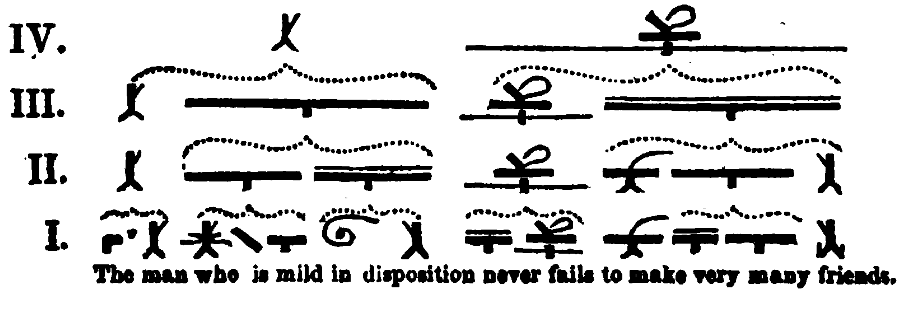
\includegraphics[width=\textwidth]{figures/vol1syntaxe2-img019.png}
    \caption{Diagramme de \citet{barnard1836analytic}}
    \small\textit{The man who is mild in disposition never fails to make very many friends.}
    ‘L’homme qui est doux de caractère n’échoue jamais à se faire de très nombreux amis.’
\end{figure}

    De la même façon, la relative \textit{who is mild in disposition} ‘qui est doux de caractère’ se comporte comme un adjectif (cf. le symbole 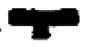
\includegraphics[height=1.4ex]{figures/vol1syntaxe2-img021.png} également associé à \textit{mild} ‘doux’ et \textit{many} ‘nombreux’) et sa combinaison avec \textit{the man} ‘l’homme’ se comporte comme un nom (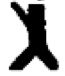
\includegraphics[height=1.25ex]{figures/vol1syntaxe2-img022.png}) ; de même, \textit{to make very many friends} ‘à se faire vraiment beaucoup d’amis’ se comporte comme un adverbe et sa combinaison avec \textit{never fails} ‘n’échoue jamais’ comme un verbe (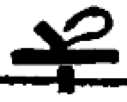
\includegraphics[height=1.5ex]{figures/vol1syntaxe2-img020.png}). Par contre Barnard ne considère pas la proposition comme équivalente au verbe et reste avec une structure sujet-prédicat pour la proposition que l’on retrouve de la grammaire de Port-Royal à la grammaire générative (voir l’encadré sur \textit{Fonctions syntaxiques et prédicat} du \chapfuturef{17}). Le diagramme qu’il propose peut néanmoins être considéré comme un premier exemple d’arbre de constituants et même d’arbre de constituants avec tête, puisque les étiquettes indiquent la catégorie de la tête comme en Syntaxe X-barre (voir l’\encadref{sec:3.4.19} sur la \textit{Syntaxe X-barre}).
    
    Il semble que les contemporains de Barnard n’aient pas vraiment vu la portée de ces diagrammes et il faut attendre plus d’un siècle pour que, en \citeyear{nida1943morphology}, dix ans après la publication de \textit{Langage} de Bloomfield, Eugene Nida propose à nouveau des structures de constituants, dans une thèse intitulée \textit{A Synopsis of English Syntax}. Les structures proposées par Nida sont en fait des polygraphes (voir l’\encadref{sec:3.2.23} sur \textit{Graphe à bulles et polygraphe}) où chaque lien représente une connexion binaire et où les liens peuvent avoir pour sommet d’autres liens. Nida va ensuite enrichir son système, dans la republication de sa thèse en \citeyear{nida1966synopsys}, en ajoutant des symboles sur les liens (voir la figure \ref{fig:nida}) : les liens marquées d’une croix ($\times$) représentent une construction exocentrique, tandis que les liens marqués d’une flèche (~$\langle$~ou~$\rangle$~) représentent une construction endocentrique, la flèche pointant vers la tête. Dans le diagramme ci-dessous, \textit{the} et \textit{men} sont connectés par un lien $\rangle$ indiquant que \textit{the} dépend de \textit{men}, puis \textit{by} est lié à ce lien par un lien $\times$ indiquant que la construction n’a pas de tête. Une telle représentation est équivalente à un arbre de constituants binaire (voir la \sectref{sec:3.4.21} sur \textit{Arbre de constituants binaire et polygraphe}).

    \begin{figure}[H]
        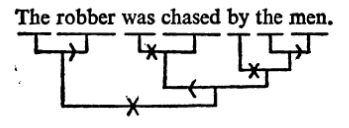
\includegraphics[width=8cm]{figures/vol1syntaxe2-img023.png}
        \caption{Représentation syntaxique de \citet{nida1966synopsys}}
        \label{fig:nida}
        \small\textit{The robber was chased by the men.} ‘Le voleur a été poursuivi par les hommes.’
    \end{figure}
     
    Une représentation similaire a été proposée dans les années 1950 par Charles Hockett (voir son ouvrage \textit{A course in modern linguistics} de \citeyear{hockett1958course}). Cette représentation, connue aujourd’hui sous le nom de \textstyleTermesapprof{boîtes de Hockett} n’est pas un arbre (au sens où les branches ne sont pas explicites), mais plutôt un emboîtement de constituants, assez proche de l’arbre de dépendance avec projections intermédiaires de la figure \ref{fig:laponie-proj}. Dans le diagramme de la figure \ref{fig:hockett1}, les unités de bases sont les syntaxèmes (on notera la décomposition de la forme verbale \textit{wants} en \textit{want}{}-\,\textrm{${\oplus}$}{}\,-\textit{s}) et les intonèmes (les «~signes~» prosodiques) sont discrétisés (c’est-à-dire représentés par des symboles, ici 2, 3, 1 et ↓) et également intégrés à la décomposition. Il s’agit en fait d’une décomposition assez proche de la structure syntaxique X-barre qui ré-émergera 20 ans plus tard (voir l’\encadref{sec:3.4.19} sur la \textit{Syntaxe X-barre}), si ce n’est que Hockett considère encore que la combinaison \textit{sujet-verbe} est endocentrique. Le diagramme peut être enrichi de symboles \tikz [baseline=(node.base)] \node[draw,circle,inner sep=0pt] (node) {<}; ou \tikz [baseline=(node.base)] \node[draw,circle,inner sep=0pt] (node) {>}; indiquant, comme chez Nida, la dépendance (voir figure \ref{fig:hockett2}).

    \begin{figure}[H]
        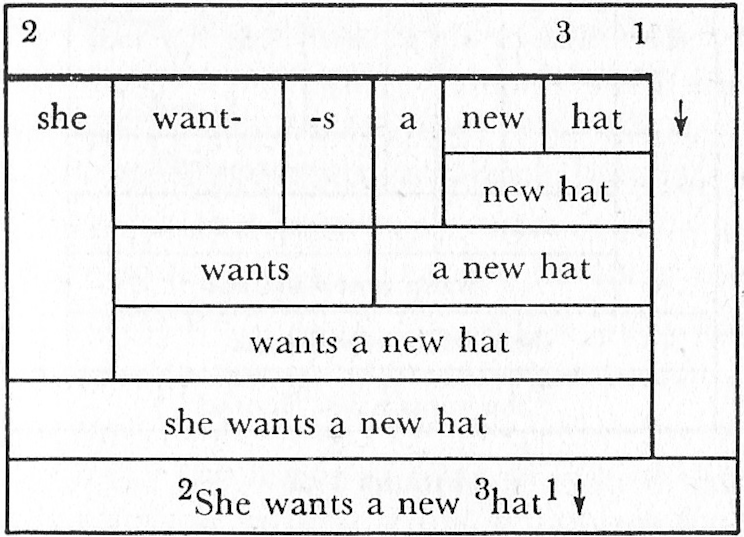
\includegraphics[width=7cm]{figures/vol1syntaxe2-img024.png}
        \caption{Boîtes de \citet[169]{hockett1958course}\label{fig:hockett1}}
        \textit{She wants a new hat.} ‘Elle veut un nouveau chapeau.’
    \end{figure}
        
    \begin{figure}[H]
        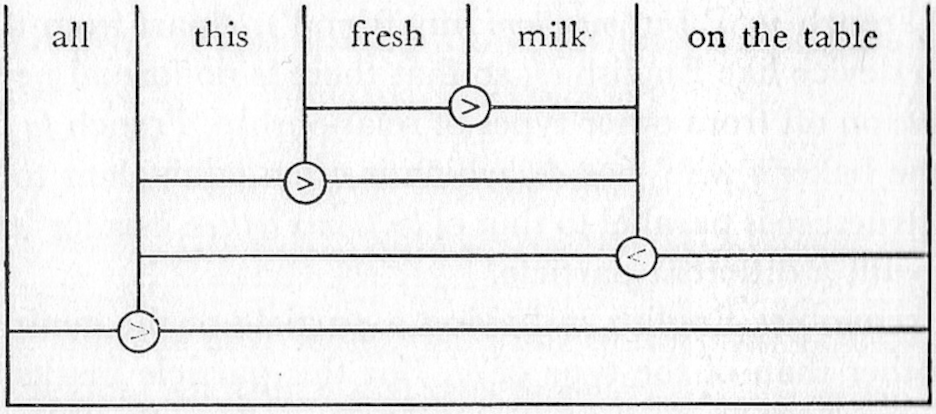
\includegraphics[width=9.5cm]{figures/vol1syntaxe2-img025.png}
        \caption{Boîtes de \cites [188]{hockett1958course} avec marquage des dépendances\label{fig:hockett2}}
        \textit{all this fresh milk on the table} ‘tout ce lait frais sur la table’
    \end{figure}

 
    Dans les représentations de Hockett, chaque module de trois cases (voir figure \ref{fig:hockett3}) est à lire comme une \hi{construction}, comme le remarque \citet[161]{hockett1958course} (dans le chapitre \textit{Form classes and constructions}). Une telle analyse est contemporaine des grammaires de réécriture de Chomsky (voir l’\encadref{sec:3.5.30} sur la \textit{Grammaire de réécriture}) et son objectif est absolument similaire. On notera néanmoins que la représentation de Hockett met autant en avant la combinaison de A et B que la relation partie-tout de A ou de B avec le tout C qu’ils forment.

    \begin{figure}[H]
    \begin{subfigure}[t]{.5\textwidth}\centering
    \begin{tikzpicture}[every node/.style={font=\strut}]
    \node at (0,0) (A) {A};
    \node at (1,0) (B) {B};
    \node at (0.5,-1.25) (C) {C};
    \node [draw,fit =(A) (B) (C)] (box) {};
    \draw (box.east) -| (box.north)
          (box.west) -| (box.north);
    \node at (box.center) [draw,circle,fill=white,inner sep=-1pt] {<};
    \end{tikzpicture}
    \caption{Construction chez Hockett}
    \end{subfigure}\begin{subfigure}[t]{.5\textwidth}\centering
        \begin{tikzpicture}
        \node [CircleFillNode] (root) {}
            child { node [CircleFillNode] {} edge from parent node [midway,anchor=east] {T} }
            child { node [CircleFillNode] {} };
        \node [above=1pt of root] {C};
        \node [below=1pt of root-1] {A};
        \node [below=1pt of root-2] {B};
        \end{tikzpicture}
        \caption{Construction dans un arbre de constituants avec tête}
    \end{subfigure}
    \caption{{Deux représentations de la même construction}\label{fig:hockett3}}
    \end{figure}   

    On attribue généralement l’introduction des arbres de constituants à Noam Chomsky. On en trouve quelques-uns dans son article de \citeyear{chomsky1955three} et un dans \textit{Syntactic Structures} de \citeyear{chomsky1957syntactic}, que nous reproduisons dans la figure \ref{fig:chomsky57}a. De manière assez surprenante, cet arbre a été remplacé, dans la réédition de 2002, par le diagramme de la figure \ref{fig:chomsky57}b. Ce nouveau diagramme n’est pas stricto sensu un arbre. Il apparaît dans le chapitre 4 intitulé \textit{Phrase structure} ‘Structure syntagmatique’, où Chomsky introduit les règles de réécriture, comme \textit{Sentence $\leftarrow$ NP $+$ VP}. Dans ce diagramme, il n’y a pas, comme dans les arbres de constituants ordinaires, de relations partie-tout entre le nœud \textit{Sentence} et les constituants immédiats \textit{NP} et \textit{VP}. Au lieu de cela, il y a un lien entre \textit{NP} et \textit{VP}, correspondant au symbole $+$ de la règle et que l’on peut interpréter comme un lien de connexion, ainsi qu’un lien entre le nœud \textit{Sentence} et le lien de connexion, correspondant à l’opération de réécriture représentée par le symbole $\leftarrow$ dans la règle. Le diagramme est donc un polygraphe.

\begin{figure}[H]
    \small
    \begin{subfigure}[b]{0.5\textwidth}
		\centering
    \begin{forest} for tree = {font=\itshape}
    [Sentence
      [NP [T [the]]
          [N [man]]
      ]
      [VP [Verb [hit]]
          [NP [T [the]]
              [N [ball]]
          ]
      ]
    ]    
    \end{forest}
    \caption{Arbre de constituant de \citeyear{chomsky1957syntactic}}
    \end{subfigure}\begin{subfigure}[b]{0.5\textwidth}
		\centering
    \begin{forest}
				for tree={
					font=\itshape,
					edge path'={}
				}
				[Sentence,name=sentence
					[NP,name=np0
						[T,name=t0
							[the,name=the0]
						]
						[N,name=n0
							[man,name=man]
						]
					]
					[VP,name=vp
						[Verb,name=verb
							[hit,name=hit]
						]
						[NP,name=np1
							[T,name=t1
								[the,name=the1]
							]
							[N,name=n1
								[ball,name=ball]
							]
						]
					]
				]
				\draw[thick] (np0.north) |- ($(np0.north)!0.5!(vp.north)+(0,9pt)$) -| (vp.north);
				\draw[thick] (t0.north) |- ($(t0.north)!0.5!(n0.north)+(0,9pt)$) -| (n0.north);
				\draw[thick] (verb.north) |- ($(verb.north)!0.5!(np1.north)+(0,9pt)$) -| (np1.north);
				\draw[thick] (t1.north) |- ($(t1.north)!0.5!(n1.north)+(0,9pt)$) -| (n1.north);
				\draw[thick] ($(sentence.south)+(0,2pt)$) -- ($(np0.north)!0.5!(vp.north)+(0,11pt)$);
				\draw[thick] ($(np0.south)+(0,2pt)$) -- ($(t0.north)!0.5!(n0.north)+(0,11pt)$);
				\draw[thick] ($(vp.south)+(0,2pt)$) -- ($(verb.north)!0.5!(np1.north)+(0,11pt)$);
				\draw[thick] ($(np1.south)+(0,2pt)$) -- ($(t1.north)!0.5!(n1.north)+(0,11pt)$);
				\draw[thick] ($(t0.south)+(0,2pt)$) -- ($(the0.north)$);
				\draw[thick] ($(n0.south)+(0,2pt)$) -- ($(man.north)$);
				\draw[thick] ($(verb.south)+(0,2pt)$) -- ($(hit.north)$);
				\draw[thick] ($(t1.south)+(0,2pt)$) -- ($(the1.north)$);
				\draw[thick] ($(n1.south)+(0,2pt)$) -- ($(ball.north)$);
			\end{forest}
			\caption{Diagramme polygraphique de l'édition de 2002}
    \end{subfigure}
    \small\textit{The man hit the ball.} ‘L'homme frappa le ballon.’
    \caption{Deux versions d'une structure de dérivation par Chomsky\label{fig:chomsky57}}
\end{figure}

Alors que la version 2002 de l'arbre de 1957 est fondamentalement binaire, la binarité n’est plus exigée dans les arbres de \textit{Aspects of the Theory of Syntax}, publié en \citeyear{chomsky1965aspects} (voir un exemple dans la figure \ref{fig:chomsky65} avec des branchements unaires, binaires et ternaires). Elle réapparaîtra dans les travaux suivants et notamment la Syntaxe X-barre.


\begin{figure}[H]
% %     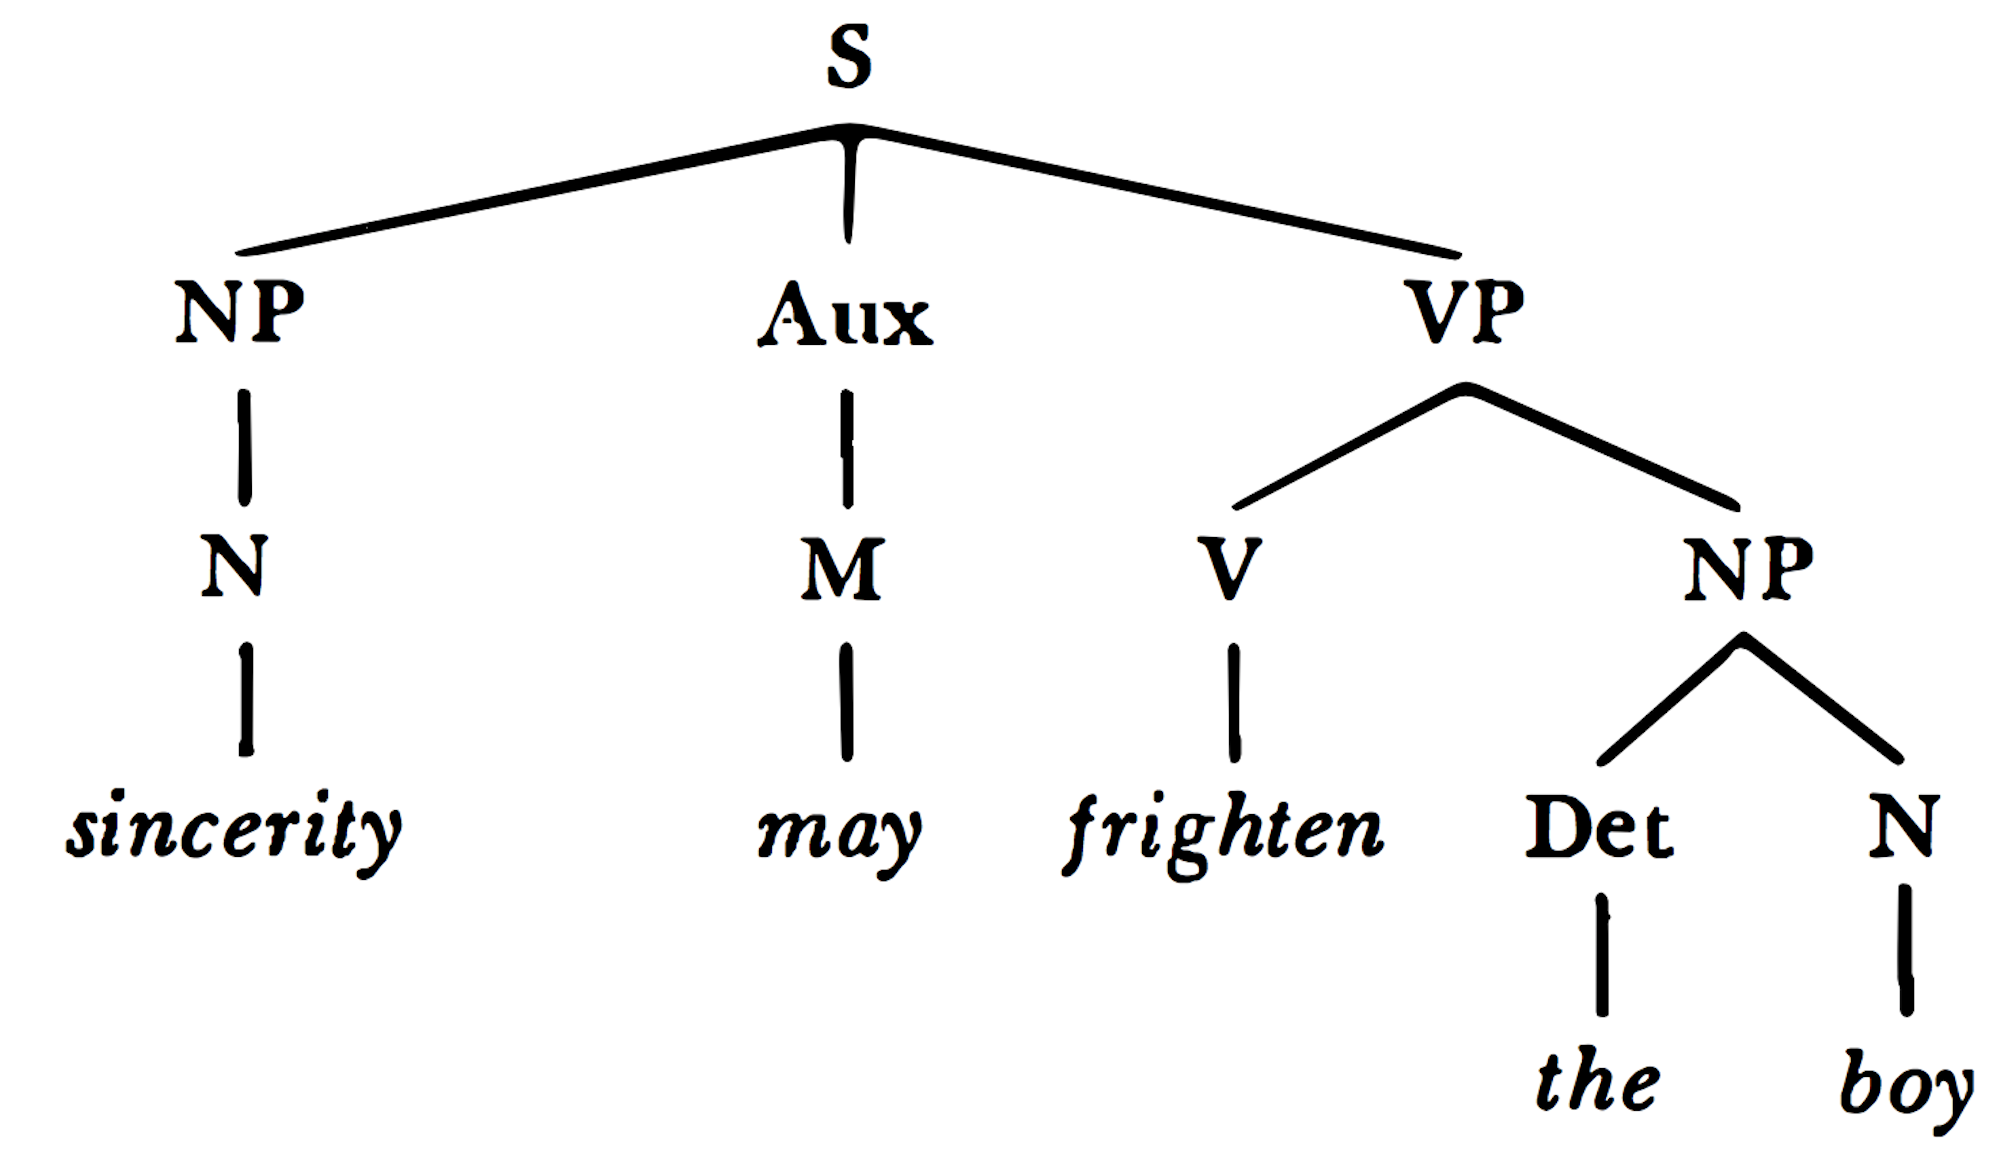
\includegraphics[width=\textwidth]{figures/vol1syntaxe2-img027.png}
   \begin{forest}
   [\normalfont S, calign=child, calign child=2
     [NP [N [\itshape sincerity]]]
     [Aux [M [\itshape may]]]
     [VP [V [\itshape frighten]]
         [NP [Det [\itshape the]]
             [N [\itshape boy]]
         ]
     ]
   ]
   \end{forest}
    \caption{Arbre syntaxique de \citet{chomsky1965aspects}\label{fig:chomsky65}}
   \small\textit{Sincerity may frighten the boy} ‘La sincérité peut effrayer le garçon’ 
\end{figure}
  }
\loupe[sec:3.4.18]{Binarité, construction et connexion}{%
    L’exigence de \textstyleTermesapprof{binarité} des arbres de constituants est antérieure à l’usage de la représentation en arbre. L’idée qu’une décomposition représente une \textstyleTermesapprof{construction} élémentaire est déjà bien présente dans \textit{Language} de Leonard \citet{bloomfield1933language}. Bloomfield donne l’exemple de la construction \textit{actor-action}, que l’on pourrait appeler la construction \textit{subjectale}, pour reprendre un terme proposé par Igor \citet{melcuk1988dependency}. Autrement dit, il existe dans la phrase ordinaire une combinaison remarquable qui est celle du sujet avec le prédicat verbal (qu’on le conçoive comme le verbe seul ou comme un «~groupe verbal~», cela ne change rien pour nous, en termes de connexion). Cette construction (il s’agit bien d’une construction, au sens où on l’entend encore aujourd’hui, par exemple dans les \textstyleTermesapprof{Grammaires de constructions}) (voir les \textit{Lectures additionnelles}) est bien binaire, mettant en relation deux éléments, le sujet et le prédicat verbal. Selon les formalismes, cette construction sera représentée par une connexion ou une décomposition (voir la figure \ref{fig:subjectale}).

 \begin{figure}[H]
    \begin{minipage}[c]{.3\linewidth}\centering
      \begin{tikzpicture} 
        \node [CircleNode,label=below:N] at (0,0) (A) {};
        \node [CircleNode,label=below:V] at (2,0) (B) {};
        \draw[-{Triangle[]}] (B) to [bend right] node [midway,above,font=\itshape] {sujet} (A);
      \end{tikzpicture}
    \end{minipage}
    \begin{minipage}[c]{.3\linewidth}\centering
      \begin{forest}
       for tree = {font=\normalfont, no edge}
       [S [NP] [VP]]
       \draw (!1) |- ++(10pt,1.15\baselineskip) -| (!2);
       \draw () -- ++(0,-1.25\baselineskip);
      \end{forest}
    \end{minipage}
    \begin{minipage}[c]{.3\linewidth}\centering
      \begin{forest} for tree = {font=\normalfont}
        [S [NP] [VP]]
      \end{forest}
    \end{minipage}    
    \caption{\label{fig:subjectale}Trois représentations de la construction subjectale}
 \end{figure}

    Le premier diagramme de la figure \ref{fig:subjectale} dit qu’il y a une unité dont la tête est un nom (N) qui dépend d’un verbe (V) par une relation \textit{sujet}, le deuxième diagramme \citep{chomsky1957syntactic} dit qu’il y a un groupe nominal (NP, \textit{noun phrase}) et un groupe verbal (VP, \textit{verbal phrase}) qui se connectent pour former ensemble une phrase (S, \textit{sentence}), tandis que le troisième diagramme dit que la phrase S possède deux composantes, un NP et un VP. Même si cela n’apparaît pas au premier regard, il s’agit de trois représentations de la même construction. Qui plus est, ces trois descriptions sont moins éloignées qu’il n’y paraît à première vue : comme on l’a déjà vu dans le \chapref{sec:3.2} sur la \textit{Connexion} et comme on le verra à nouveau dans la \sectref{sec:3.4.21} sur \textit{Arbre de constituants binaire et polygraphes}, on passe de l’une à l’autre en réifiant ou déréifiant les relations partie-tout de la relation \textit{sujet}.

    L’exigence de binarité est une propriété partagée par de nombreuses analyses en constituants et par les analyses en dépendance : de la même façon que les constructions sont encodées, dans un arbre de dépendance, par des \hi{dépendances}, c’est-à-dire des \hi{relations liant deux à deux des mots}, les constructions seront encodées, dans un arbre de constituants binaire, par des \hi{décompositions binaires}, c’est-à-dire des \hi{combinaisons deux à deux de constituants}, .

    La principale différence entre les deux approches concerne la façon dont les différentes constructions sont repérées dans la structure. Dans le cadre de la syntaxe de dépendance, les constructions sont distinguées par l’étiquetage fonctionnel des dépendances (voir le \chapfuturef{17} sur les \textit{Relations syntaxiques}) et donc par une dénomination explicite de la construction : ainsi l’étiquette \textit{sujet} sur la dépendance plus haut indique qu’il s’agit de la construction subjectale. Dans le cadre de la syntaxe de constituants, les primitives sont les catégories et le repérage entre les constructions est fait par la configuration et les catégories : ainsi le sujet est le NP sous S, tandis que l’objet est le NP sous VP (voir la figure \ref{fig:objectale} qui compare les deux modes de représentation).

\begin{figure}[H]
  \begin{minipage}[c]{.3\linewidth}\centering
     \begin{forest} for tree = {font=\normalfont}
       [S [NP] [VP [V] [NP]]]
     \end{forest}
    \end{minipage}\hfill\begin{minipage}[c]{.6\linewidth}\centering
    \begin{tikzpicture}
      \node at (0,0) [CircleNode,label=below:N] (A) {};
      \node at (2,0) [CircleNode,label=below:V] (B) {};
      \node at (4,0) [CircleNode,label=below:N] (C) {};
      \path [-{Triangle[]}] (B) edge [bend right] node [midway,above,font=\itshape]
        {sujet} (A)
                                edge [bend left] node [midway,above,font=\itshape]
        {objet} (C);
    \end{tikzpicture}
    \end{minipage}
   \caption{\label{fig:objectale}Deux représentations des constructions subjectale et objectale}
\end{figure}
}
\loupe[sec:3.4.19]{Syntaxe X-barre}{%
    La \textstyleTermesapprof{Syntaxe X-barre} est la version la plus aboutie de l’\hi{analyse en constituants immédiats} (ACI) (voir la \sectref{sec:3.2.25} éponyme). Elle est développée à partir des années 1970 par Noam Chomsky et son étudiant Ray Jackendoff.

    L’innovation majeure de la Syntaxe X-barre est que \hi{tout constituant} est considéré comme étant la \hi{projection d’une} \hi{tête}. Dans les versions précédentes de l’ACI, la phrase était décomposée en un groupe substantival et un groupe verbal (cf. la fameuse règle S \textrm{→} NP VP), ce qui en faisait un constituant exocentrique. Le fait que tout constituant ait une tête rend la Syntaxe X-barre extrêmement proche d’une analyse en dépendance. (Seule la coordination est encore parfois traitée comme une construction symétrique dont les conjoints sont les co-têtes ; voir \encadref{sec:3.4.26} sur les \textit{Deux types d’arbres de constituants}.)

    La deuxième caractéristique de la Syntaxe X-barre est que les \hi{nœuds} \hi{de base} sont des \hi{syntaxèmes} et non des mots. Il y a donc deux types de constituants considérés, les \hi{projections lexicales}, dont la tête est un lexème, et les \hi{projections} dites \hi{fonctionnelles} dont la tête est un syntaxème flexionnel (une catégorie fonctionnelle dans les termes de la Syntaxe X-barre).

    La troisième caractéristique de la Syntaxe X-barre est que l’arbre de constituants est \hi{ordonné} et aucun constituant n’est discontinu, ce qui, pour les raisons que nous avons exposé dans l’\encadref{sec:3.2.7} \textit{De la non-séparation des ordres au mouvement}, entraîne la présence de nombreuses positions occupées par des traces co-indicés avec d’autres positions.

    La quatrième caractéristique de l’arbre X-barre est qu’il est \hi{binaire}. Ainsi la combinaison de chaque dépendant avec son gouverneur correspond à une décomposition binaire différente, ce qui, d’une certaine façon, rapproche encore plus cet arbre d’un arbre de dépendance (voir l’\encadref{sec:3.4.18}). La conséquence est que si un syntaxème a beaucoup de dépendants, il sera la tête d’autant de projections. Si le syntaxème est de catégorie X, sa \hi{projection maximale} est notée XP (\textit{X Phrase}) et ses \hi{projections intermédiaires} X’ (à l’origine elles étaient notées $\overline{\text{X}}$, avec une ou plusieurs barres au-dessus de X, d’où le nom de Syntaxe X-barre).

    La Syntaxe X-barre considère de plus que l’élément sous XP a des propriétés différentes des éléments sous X’ : le premier est un \hi{spécifieur}, alors que les autres sont des \hi{compléments} (figure \ref{fig:Xbarre}). Dans certaines versions de la Syntaxe X-barre \citep{jackendoff1977x}, les ajouts (ou modifieurs) sont structurellement distingués des compléments actanciels par l’ajout d’un niveau de stratification supplémentaire dans la configuration de base (c’est-à-dire que XP porte une «~barre~» supplémentaire).

\begin{figure}[H]
    \begin{forest} for tree = {font=\normalfont}
    [XP,calign=child, calign primary child=2
        [spécifieur] [X', calign=child, calign primary child=1
            [X] [complément]
        ]
    ]
    \end{forest}
     \caption{Configuration de base de la Syntaxe X-barre}
    \label{fig:Xbarre}
\end{figure}

    En conclusion, l’arbre de constituants de la Syntaxe X-barre est assez différent des arbres de constituants plats. Les deux sont des \hi{arbres de constituants avec têtes}, mais le dernier ne contient que des projections maximales, qui, qui plus est, peuvent former des constituants discontinus. L’arbre X-barre ne repose pas vraiment sur des tests de constituance (qui, comme on l’a vu dans l'\encadref{sec:3.4.11}, caractérisent essentiellement les projections maximales), mais sur des \hi{principes configurationnels}. En d’autres termes, plus la géométrie d’un arbre permet de prédire de propriétés syntaxiques de l’énoncé qu’il représente, plus l’arbre a de raisons d’être. Ainsi, par exemple, le fait que le groupe substantival qui suit \textit{mange} possède des propriétés différentes dans les deux phrases suivantes devrait conduire à des configurations différentes, ce qui amène à compliquer à dessein la structure :

\ea
\ea   \textit{Pierre mange le pain.}
\ex   \textit{Pierre mange la nuit.} 
\z
\z

    Dans l’approche que nous développons ici, ces deux énoncés auront la même «~structure~» syntaxique (c’est-à-dire le même squelette structurel), mais les groupes substantivaux \textit{le pain} et \textit{la nuit} auront des fonctions totalement différentes (voir le \chapfuturef{17} sur les \textit{Relations syntaxiques}).

    On peut s’étonner du fait que la Syntaxe X-barre, dont l’objectif est de rendre compte des propriétés syntaxiques par des configurations géométriques, n’ait pas cherché à encoder structurellement une notion aussi fondamentale que la notion de \textit{tête}, ce que font pourtant assez simplement les structures de dépendance !
}
\loupe[sec:3.4.20]{Le groupe verbal}{%
    Le terme \textit{groupe verbal} (angl. \textit{verb phrase}, \textit{VP}) n’est pas utilisé de manière consistante dans la littérature. Ce terme désigne selon les auteurs deux notions différentes, que nous appellerons VP1 et VP2 :

    \begin{itemize}
    \item VP1 est une \hi{projection partielle} de la \hi{forme verbale} sans son sujet ;
    \item VP2 est la \hi{projection maximale} du \hi{lexème verbal}.
    \end{itemize}
    Les deux notions sont souvent confondues, alors qu’elles renvoient à des constituants différents (voir la figure \ref{fig:VP1VP2}) et à des cadres théoriques différents.

    VP2 est une notion théoriquement valable, mais qui suppose que l’on travaille avec la \hi{granularité des syntaxèmes}. Il y a alors lieu de considérer que le sujet dépend plutôt de la flexion (voir la \sectref{sec:3.2.18} \textit{Structures de connexion, granularité et critères}) et donc la \hi{projection maximale du lexème verbal} est bien VP2, c'est-à-dire un constituant qui ne contient pas le sujet. On notera néanmoins que VP2 n’est pas une unité autonomisable (puisque le lexème verbal n’apparaît jamais sans flexion) et qu’elle n’est donc qu’un objet théorique servant à expliciter, dans le cadre de l’analyse en constituants, que la réalisation du sujet est davantage liée à la nature de la flexion qu’à celle du lexème. Il y a, à notre avis, des moyens plus simples et plus directs d’indiquer le lien entre le sujet et la désinence verbale.

    VP1 est une notion sans grand intérêt théorique de notre point de vue. Il s’agit d’un constituant intermédiaire (VP1 est le I’ de l’analyse de droite de la figure \ref{fig:theo-Xbarre}), qui résulte d’une stratification qui nous semble peu justifiée. En effet, rien ne permet de considérer que la forme verbale se combine d’abord avec ses autres dépendants avant de se combiner avec son sujet et donc de donner ainsi un statut spécial au sujet.

\begin{figure}[H]
\hfill
      \begin{multicols}{2}\raggedcolumns
    \begin{forest} for tree = {font=\normalfont}
     [S  [<\textit{sujet}>] [VP1 [\hspaceThis{VP1},roof]]]
    \end{forest}
    \hfill
    \begin{forest}
     [IP [<\textit{sujet}>] [I' [I [<\textit{flexion}>]] [VP2 [\hspaceThis{VP2},roof]]]]
    \end{forest}
    \end{multicols}\hfill
    \caption{\label{fig:VP1VP2}Configurations syntaxiques caractérisant respectivement VP1 et VP2}
\end{figure}

    Dernière remarque qui pourrait expliquer l’introduction de VP1 dans les analyses en constituants : l’anglais (qui est la langue la plus étudiée et la plus enseignée) a un \hi{constituant topologique} du type VP1 (voir les \textit{Exercices} du \chapref{sec:3.5}). Mais il est clair que la plupart des langues n’ont pas du tout cette configuration topologique et que, de toute façon, cela ne justifie pas l’introduction de VP1 dans la structure syntaxique au sens propre (que nous distinguons de la structure topologique).
}
\section{Arbre de constituants binaire et polygraphe}\label{sec:3.4.21}

Nous avons vu deux usages possibles de la représentation de la structure syntaxique par un arbre de constituants avec têtes : l’\hi{arbre de constituants plat} et l’\hi{arbre de constituants binaire}. (Nous confirmerons qu’il s’agit bien de deux usages différents du même formalisme dans l’\encadref{sec:3.4.25} sur \textit{Deux types d’arbres de constituants}, où nous montrons l’interprétation différente du branchement ternaire dans les deux conventions de représentation).

Nous avons vu que l’arbre de constituants plat pouvait être déduit trivialement (c’est-à-dire par un procédé de conversion automatique pure, sans ajout d’aucune information) d’un arbre de dépendance, ce qui n’est pas le cas de l’arbre de constituants binaire, qui nécessite d’ajouter un ordre de saillance sur les dépendances. Cela pourrait laisser penser que l’arbre de constituants plat est plus proche de l’arbre de dépendance : c’est vrai si on se place du point de vue formel, mais ça ne l’est pas si on se place du point de vue théorique. Comme on l’a vu dans l'\encadref{sec:3.4.15}, il y a derrière l’\hi{exigence de binarité}, le souci de dégager les différentes constructions syntaxiques, de les isoler les unes des autres. Et ce souci est commun avec les grammaires de dépendances. Nous allons montrer cela maintenant en repartant de l'exemple \REF{ex:laponie2} et de son arbre binaire le plus standard, donné dans la figure \ref{fig:laponie-T2}.

On peut interpréter chaque branchement binaire comme une connexion entre deux unités. Comme nous l’avons vu à la \sectref{sec:3.2.12} \textit{Représenter les combinaisons}, on peut représenter la combinaison A ${\oplus}$ B aussi bien par un lien entre A et B que par une bulle entourant A et B. Passer à un branchement binaire revient à \hi{réifier} les relations partie-tout entre A et B et l’unité qu’ils forment ensemble (voir l’\encadref{sec:3.4.22} qui suit pour des compléments sur la notion de réification). Ici nous proposons de faire l’inverse, c’est-à-dire de \hi{déréifier} les relations partie-tout qui constituent les branches d’un arbre de constituants. Comme, en plus, chaque branchement binaire indique une tête (la branche T), la déréification permet de récupérer une connexion orientée, c’est-à-dire une dépendance. Ceci est illustré dans la figure \ref{fig:dereification}.

\begin{figure}

\begin{tikzpicture}
  \node at (0,0) (A)  [CircleFillNode,label=below:A] {};
  \node at (2,0) (B)  [CircleFillNode,label=below:B] {};
  \node at (1,1) (U) [CircleFillNode,label=above:U] {};
  
  \draw (A) -- node [midway,anchor=base east] {T} (U)
            -- (B);

 \node at (3,0.5) {\huge$\Leftrightarrow$};
 \node at (4,0) (A2)  [CircleFillNode,label=below:A] {};
 \node at (6,0) (B2)  [CircleFillNode,label=below:B] {};
 \draw[-{Triangle[]}] (A2) to [bend left] node [midway,above] {U} (B2);
\end{tikzpicture}

\caption{\label{fig:dereification}Passage d’un branchement binaire à une dépendance par déréification d’un nœud non terminal}
\end{figure}

Si l’on applique la déréfication à tous les nœuds intérieurs de l’arbre de constituants binaire de la figure \ref{fig:laponie-T2}, on obtient la structure de la figure \ref{fig:polygraphe-ordre}. Cette structure est un \textstyleTermes{polygraphe} (voir définition formelle dans l’\encadref{sec:3.2.23} sur \textit{Graphe à bulles et polygraphe}) : ce n’est pas exactement un graphe, puisqu’un arc ne lie pas forcément deux nœuds (les nœuds sont les mots), mais il peut lier d’autres arcs entre eux ou un arc et un nœud. De plus, ce polygraphe est \textstyleTermes{orienté}, puisque chaque arc du graphe lie un gouverneur à un dépendant. Enfin ce polygraphe est implicitement \textstyleTermes{ordonné}, dans le sens où les nœuds du polygraphe sont disposés selon un ordre linéaire (celui des mots dans la phrase). De telles structures ont été proposées par le linguiste américain Eugene Nida dans sa thèse soutenue en \citeyear{nida1943morphology} (voir l’\encadref{sec:3.4.17} sur l’\textit{Historique des représentations syntaxiques par des diagrammes en constituants}.)

\begin{figure}
\caption{\label{fig:polygraphe-ordre}Polygraphe orienté et ordonné}
\begin{forest} for tree = {edge={draw=none},font=\itshape, fit=band}
[
 [ [beaucoup] [ [de] [gens] ] ]
 [ [aimeraient]
        [,before drawing tree={y-=2.5mm}
          [ [passer] [Noël] ] 
          [ [en] [Laponie] ] 
        ] 
  ]
]
\begin{scope}[>={Triangle[]},overlay]
\draw[->] (!2.north)    to [bend right=60] (!1.south);
\draw[->] (!11.north)   to [bend left=60]  (!12.south);
\draw[->] (!121.north)  to [bend left=60]  (!122.north);
\draw[->] (!21.north)   to [bend left=60]  (!22.south);
\draw[->] (!221.south)  to [bend left=60]  (!222.south);
\draw[->] (!2211.north) to [bend left=60]  (!2212.north);
\draw[->] (!2221.north) to [bend left=60]  (!2222.north);
\end{scope}
\end{forest}
\end{figure}

\maths[sec:3.4.22]{Réification et transitivité}{%
    Nous appelons \textstyleTermes{réification}, du latin \textit{res} ‘chose’, l'opération qui consiste à rendre concret un élément virtuel d'une structure, comme un point de contact entre deux objets. Pour mieux comprendre ce qu'est la réification, donnons un autre exemple, emprunté à la représentation sémantique des constructions transitives. Considérons une phrase élémentaire telle que :

    \ea\label{ex:frappe}
    \textit{Marie frappe Pierre.}
    \z
 Il y a là ce qu’on appelle un verbe transitif, \textit{frappe}, qui exprime une action d’un élément (\textit{Marie}) sur un autre (\textit{Pierre}). On dira encore que \textit{Marie} est l’\hi{agent} de l’action et \textit{Pierre} le \hi{patient}. Il y a alors plusieurs façons de représenter graphiquement le «~sens~» de cette phrase. Nous en proposons trois dans la figure \ref{fig:frappe-reif}.

\begin{figure}[H]
    \begin{subfigure}[t]{.5\textwidth}\centering
      \begin{tikzpicture}
        \node at (0,0) [ConcSet] (Marie) {Marie};
        \node [right=1mm of Marie, draw, signal, signal to=east, font=\itshape] (frappe) {frappe}; 
        \node [right=1mm of frappe, ConcSet] (Pierre) {Pierre};
      \end{tikzpicture}
      \caption{Sans réification des relations}
      \end{subfigure}\begin{subfigure}[t]{.5\textwidth}\centering
      \begin{tikzpicture}
        \node at (0,0) [ConcSet] (frappe) {frappe};
        \node at (-1.5,-1.5) [ConcSet] (Marie) {Marie};
        \node at (1.5,-1.5) [ConcSet] (Pierre) {Pierre};
        \draw[-{Triangle[]}] (frappe) -- (Marie)  node [near start, font=\footnotesize, left] {agent};
        \draw[-{Triangle[]}] (frappe) -- (Pierre) node [near start, font=\footnotesize, right] {patient};
      \end{tikzpicture}
      \caption{Avec réification des relations}
      \end{subfigure}\medskip\\\begin{subfigure}[t]{.5\textwidth}\centering
      \begin{tikzpicture}
        \node at (0,0) [ConcSet] (frappe) {frappe};
        \node at (-1.5,-3.15) [ConcSet] (Marie) {Marie};
        \node at (1.5,-3.15) [ConcSet] (Pierre) {Pierre};
        \node at (-1.5,-1.4) [draw,rectangle] (agent) {agent};
        \node at (1.5,-1.4) [draw,rectangle] (patient) {patient};
        \draw[-{Triangle[]}] (agent) edge node[midway,left, font=\footnotesize] {2} (frappe)
                                     edge node[midway,left, font=\footnotesize] {1} (Marie);
        \draw[-{Triangle[]}] (patient) edge node[midway,right, font=\footnotesize] {2} (frappe)
                                       edge node[midway,right, font=\footnotesize] {1} (Pierre);
      \end{tikzpicture}
      \caption{Avec réification des liens entre relations et sens lexicaux}
      \end{subfigure}
  \caption{\label{fig:frappe-reif}Trois niveaux de réification pour la représentation du sens de \REF{ex:frappe}}
\end{figure}

    Dans la représentation a, \textit{frappe} est directement modélisé comme une action de Marie sur Pierre : \textit{frappe} (\textit{Marie}, \textit{Pierre}). Dans la représentation b, les relations qui lient \textit{frappe} à \textit{Marie} et \textit{Pierre} sont explicitées et nommées \textit{agent} et \textit{patient}. Dans la représentation c, les relations agent et patient sont vues comme des objets à part entière reliant les mots de la phrase : agent~(\textit{Marie}, \textit{frappe}) + patient~(\textit{Pierre}, \textit{frappe}). On l’aura deviné, les trois représentations sont des réifications successives des relations d’une même structure.

    Si toute structure peut-être réifiée à l’infini, comment choisir le bon niveau de réification ? Faire de la relation entre deux objets un objet n’a d’intérêt que si l’on veut considérer cet objet en tant que tel et lui attribuer des propriétés. Dans le cas de la transitivité, on peut préférer la représentation b qui explicite les relations d’agent et de patient et permet donc d’en parler, par exemple pour décrire la voix passive (voir le \chapref{sec:13}).

    Dans le cas de la relation de connexion, nous pensons qu’il n’est pas nécessaire d’expliciter les relations partie-tout que la connexion entretient avec les unités qu’elle connecte, d'autant que la connexion est pour nous une classe d'équivalence de combinaisons qui mettent en jeu des unités de granularité variée (voir la \sectref{sec:3.2.14} sur \textit{La connexion et ses instances}).}

\section{Polygraphe orienté et arbre de dépendance}\label{sec:3.4.23}

Si l’on s’abstrait complètement de l’ordre linéaire et que l’on garde uniquement le polygraphe orienté, on peut adopter la représentation de la figure \ref{fig:laponie-polygraphe-pur}, où chaque arc est représenté par une ligne droite avec le gouverneur au-dessus de son dépendant.

\begin{figure}
\caption{\label{fig:laponie-polygraphe-pur}Polygraphe orienté (non ordonné)}
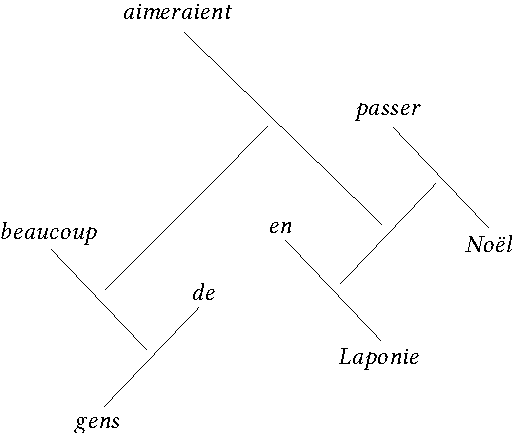
\includegraphics[scale=0.9]{figures/polygraphs/poly-3.4.23-1.pdf}
\end{figure}

Bien que cela n’apparaisse pas au premier coup d’œil, cette structure est un extrait de la structure de la figure \ref{fig:polygraphe-ordre} : c’est le même \hi{polygraphe orienté} que précédemment, mais sans l’ordre des mots et avec une autre convention de représentation. Au lieu d’indiquer la hiérarchisation de la connexion par une flèche, celle-ci est indiquée en plaçant le gouverneur au-dessus du dépendant. Or ce polygraphe orienté, qui a donc été extrait automatiquement de l’arbre de constituants binaire en mettant en évidence les connexions, est très proche d’un arbre de dépendance. Pour obtenir l’arbre de dépendance, il suffit de \hi{faire glisser chaque dépendance} le long des dépendances sur lesquelles elle s’appuie, comme montré dans la figure \ref{fig:glissade}. Nous retombons ainsi sur l'arbre de dépendance de départ (voir figure \ref{fig:laponie-dep2}).

\begin{figure}
\begin{minipage}{.45\textwidth}\centering
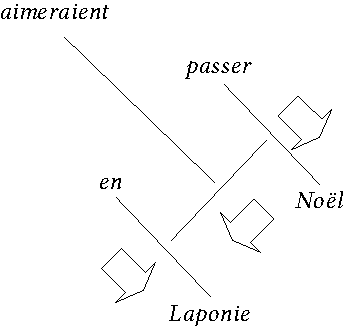
\includegraphics[scale=0.9]{figures/polygraphs/poly-3.4.23-2.pdf}
\end{minipage}\hfill%
\begin{minipage}{.05\textwidth}\centering
\huge$\Rightarrow$
\end{minipage}\hfill%
\begin{minipage}{.45\textwidth}\centering
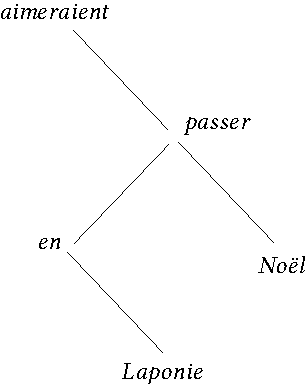
\includegraphics[scale=0.9]{figures/polygraphs/poly-3.4.23-3.pdf}
\end{minipage}
\small
\caption{\label{fig:glissade}Passage du polygraphe orienté à un arbre de dépendance par «~glissade~»}
\end{figure}



Nous appellerons \textstyleTermes{méthode par déréification }la méthode que nous venons de présenter, qui permet de passer d’un arbre de constituants binaire avec têtes à un arbre de dépendance. La méthode par déréification peut s’appliquer à des arbres de constituants dont certains branchements décrivent des constructions exocentriques et n’ont donc pas de marquage de la tête. Dans l’exemple \textit{le petit chien dort} (déjà étudié dans la \sectref{sec:3.3.23} \textit{Nom ou déterminant comme tête} ?), si l'on ne décide pas qui de l’article \textit{le} ou du nom \textit{chien} est la tête du groupe substantival, on obtient par déréification une connexion non orientée, qu’on ne peut pas faire «~glisser~» comme on l’a fait précédemment pour les connexions orientées. Comme le montre la figure \ref{fig:lechien2}, nous retombons sur le polygraphe de la figure \ref{fig:lechien}, que nous avions proposé pour l'analyse d'une construction exocentrique.

\begin{figure}
\begin{minipage}[c]{.45\textwidth}\centering
\begin{tikzpicture}[every node/.style={font=\strut}]
    \begin{scope}[
    every node/.style={CircleFillNode},
    sibling distance=15mm,
    level distance=2\baselineskip
    ]
        \node (root) {}
            child { node { } 
                    child { node { } }
                    child { node { } 
                        child { node { } }
                        child { node { } edge from parent node [reset shape, midway,anchor=base west] {T} }
                    }
                   }
            child { node { } edge from parent node [reset shape, midway, anchor=base west] {T} };
    \end{scope}
    \begin{scope}[every node/.style={font=\strut\itshape}]
    \foreach \pos/\text in {1-1/le, 1-2-1/petit, 1-2-2/chien, 2/dort} 
      {\node [below=1pt of root-\pos] {\text};}
    \end{scope}
    \end{tikzpicture}
    \end{minipage}
    \hfill%
      \begin{minipage}[c]{.05\textwidth}\centering
        \huge$\Rightarrow$
      \end{minipage}
    \hfill%
    \begin{minipage}[c]{.33\textwidth}\centering
    \begin{forest} for tree={font=\itshape}
    [dort,name=dort, s sep=2em, xshift=-4pt
        [le, no edge, name=le] [chien, no edge, name=chien [petit]]
    ]
    \draw (le) -- (chien);
    \draw (dort) -- ++ (0,-2.5em);
    \end{forest}
    \end{minipage}\hfill
\caption{\label{fig:lechien2}Conversion d'un arbre de constituants avec marquage partiel des têtes en une structure de dépendance par la méthode de déréification}
\end{figure}

\section{Comparaison des méthodes par décomposition}\label{sec:3.4.24}

Nous avons présenté deux \hi{méthodes par décomposition} pour passer d’un arbre de constituants à un arbre de dépendance : la méthode de Lecerf ou méthode par agrégation des projections d’une part et la méthode par déréification d’autre part.

Les deux méthodes sont différentes et s’appliquent à des types d’arbres de constituants différents : la \hi{méthode de Lecerf} s’applique uniquement à des arbres de constituants avec têtes, puisqu’elle repose crucialement sur l’agrégation des projections d’une même \hi{tête~}; la \hi{méthode par déréification} s’applique à n’importe quel type d’arbre de constituants, mais elle ne donne des \hi{connexions binaires} que si elle est appliquée à un arbre binaire (voir l’\encadref{sec:3.4.26} pour le cas des branchements ternaires).

Néanmoins lorsque les deux méthodes sont appliquées à un arbre de constituants \hi{binaire avec têtes}, elles donnent le \hi{même arbre de dépendance} (voir \textit{Exercices}).

\section{Équivalences entre structures}\label{sec:3.4.25}

Nous avons présenté un grand nombre de structures plus ou moins équivalentes. La figure \ref{fig:rosace} rassemble ces différentes structures.

La partie droite de la figure montre le passage d’un arbre de dépendance à \hi{un arbre de constituants plat}, puis retour à l’arbre de dépendance, tandis que la partie gauche montre le passage d’un arbre de dépendance à un \hi{arbre de constituants binaire avec têtes}, puis retour à l’arbre de dépendance.

\begin{figure}
\caption{\label{fig:rosace}Équivalence entre les différentes représentations de la structure syntaxique de \REF{ex:laponie2}}
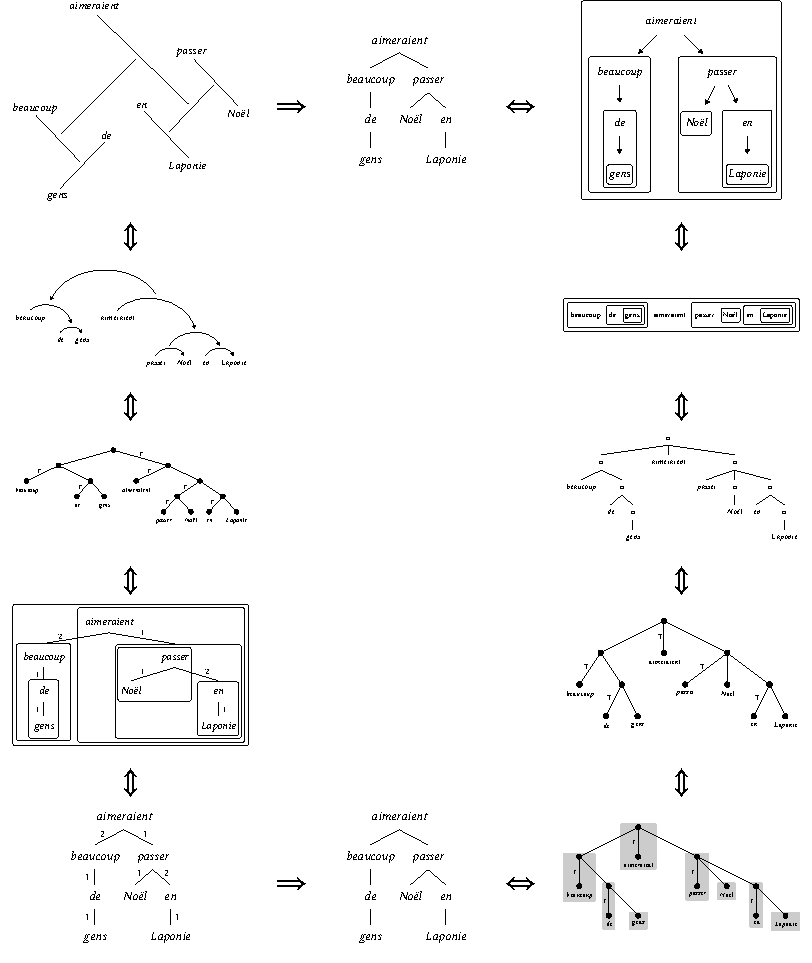
\includegraphics[width=\textwidth]{figures/graphs-collection.pdf}
\end{figure}

Chaque flèche $\Rightarrow$ ou $\Leftrightarrow$ entre deux structures symbolise une opération de conversion élémentaire permettant de passer d’une structure à une autre. Dans la plupart des cas, l’opération ne nécessite l’ajout d’aucune information et les deux structures sont équivalentes (nous ne considérons pas l’ordre linéaire sur les mots qui est des fois présent dans la structure et d’autres fois non). C’est le cas dans toute la partie droite de la figure, où toutes les structures sont équivalentes entre elles. Il s'agit de \hi{structures de constituants plates}. De la même façon, toutes les structures de la partie gauche sont équivalentes entre elles. Il s'agit de \hi{structures de constituants binaires avec têtes}. Elles contiennent une information supplémentaire qui est la stratification. Cette stratification, qui permet de stratifier les branchements non binaires, est indiquée dans la partie basse de la figure par l’ajout de l’ordre de saillance, lequel disparaît dans la partie haute, lorsque les «~glissades~» sont effectuées sur le polygraphe et qu’on revient à l’arbre de dépendance.

\loupe[sec:3.4.26]{Deux types d’arbres de constituants}{%
    Nous avons présenté dans ce chapitre deux types d’arbres de constituants avec têtes : les arbres de constituants plats et les arbres de constituants binaires comme ceux de la Syntaxe X-barre. On peut penser que tout arbre de constituants plat peut être «~binarisé~» en introduisant des constituants intermédiaires. En fait, la différence est plus profonde et il s’agit à notre avis de deux façons assez différentes d’utiliser le même formalisme. La différence apparaît lorsqu’on regarde les branchements ternaires.

    Dans un arbre plat, les branchements ternaires sont courants. Ils apparaissent dès qu’un mot a au moins deux dépendants. Reprenons l’exemple de \textit{passer Noël en Laponie}, qui se décompose en trois morceaux, une tête (\textit{passer}) et ses deux dépendants (\textit{Noël} et \textit{en Laponie}) (voir la \sectref{sec:3.4.4} sur les \textit{Arbres de constituants avec têtes}).

\begin{figure}[H]
    \begin{minipage}[c]{.45\linewidth}\centering
    \begin{tikzpicture}[every node/.style={font=\strut}]
    \begin{scope}[
    every node/.style={CircleFillNode},
    sibling distance=15mm,
    level distance=2\baselineskip
    ]
        \node (root) {}
            child { node { } edge from parent node [reset shape, midway,anchor=base east] {T} } 
            child { node { } }
            child { node { } 
                child { node { } edge from parent node [reset shape, midway,anchor=base east] {T} }
                child { node { } }
                };
    \end{scope}
    \begin{scope}[every node/.style={font=\strut\itshape}]
    \foreach \pos/\text in {1/passer, 2/Noël, 3-1/en, 3-2/Laponie} 
      {\node [below=1pt of root-\pos] {\text};}
    \end{scope}
    \end{tikzpicture}
    \end{minipage}%
    \begin{minipage}[c]{.1\textwidth}\centering
    \huge$\Leftrightarrow$
    \end{minipage}%
    \begin{minipage}[c]{.45\textwidth}\centering
    \begin{forest} for tree={font=\itshape}
    [passer
      [Noël]
      [en [Laponie]]
    ]
    \end{forest}
    \end{minipage}
 \caption{\label{fig:laponie-ternaire}Branchement ternaire et correspondance par la méthode de Lecerf}
\end{figure}

    En appliquant la méthode de Lecerf à l’arbre plat à gauche de la figure \ref{fig:laponie-ternaire}, on obtient l’arbre de dépendance à droite. Comme on le voit, le branchement ternaire est interprété comme deux connexions binaires, la connexion entre \textit{passer} et \textit{Noël} et la connexion entre \textit{passer} et \textit{en Laponie}.

    Dans un arbre binaire, il en va tout autrement, puisque, comme nous l’avons montré ci-dessus (\sectref{sec:3.4.21} sur \textit{Arbres de constituants binaire et polygraphe}), \hi{chaque branchement correspond à une unique connexion}. Si un tel arbre contient un branchement ternaire, il doit être interprété comme une \hi{connexion ternaire} (voir l’\encadref{sec:3.2.17} éponyme). La Syntaxe X-barre, qui revendique l’usage des arbres binaires, s’est aventurée à proposer des branchements ternaires pour la coordination (notamment dans l'ouvrage de \citealt{jackendoff1977x}). On trouve déjà les mêmes arbres dans \citealt{hockett1958course} ; cf.\ la figure \ref{fig:hockett-coord} les boîtes de Hockett pour la coordination où le branchement est ternaire et symétrique, avec une position bien différenciée pour la conjonction).

\begin{figure}[H]
%     \includegraphics{}
    \caption{\label{fig:hockett-coord}Branchement ternaire dans une boîte de Hockett}
     \todo[inline]{Structure of this graph could not be obtained from the original submission file}
    \todo[inline]{I drew it. Is it possible to draw it again?}
\end{figure}


Cette analyse est ce qu’on appelle l’\hi{analyse symétrique de la coordination} (voir le \chapfuturef{18}) : dans \textit{Marie et Pierre dorment}, les conjoints (c’est le nom que l’on donne aux éléments coordonnés, \textit{Marie} et \textit{Pierre}) sont considérés comme des co-têtes, qui contribuent à égalité à la distribution du syntagme (lequel déclenche un accord pluriel du verbe). Il s’agit alors d’une construction ternaire, que nous pouvons représenter par une connexion ternaire en suivant les conventions de représentation utilisées par Tesnière dans son article de \citeyear{tesniere1934comment} \textit{Comment construire une syntaxe ?} : les deux conjoints \textit{Marie} et \textit{Pierre} sont au même niveau, reliés par une connexion horizontale, et la conjonction, qui est le troisième «~sommet~» de cette connexion, est placé en dessous.

\begin{figure}[H]
    \begin{minipage}[c]{.55\linewidth}\centering
    \begin{tikzpicture}[every node/.style={font=\strut}]
    \begin{scope}[
    every node/.style={CircleFillNode},
    level 1/.style={sibling distance=30mm},
    level 2/.style={sibling distance=15mm},
    level distance=2\baselineskip
    ]
        \node (root) {}
            child { node { } 
                child { node { } edge from parent node [reset shape, midway, anchor=base east] {T} }
                child { node { } }
                child { node { } edge from parent node [reset shape, midway, anchor=base west] {T} }
                  }
            child { node { } edge from parent node [reset shape, midway, anchor=base west] {T} }; 
    \end{scope}
    \begin{scope}[every node/.style={font=\strut\itshape}]
    \foreach \pos/\text in {1-1/Marie, 1-2/et, 1-3/Pierre, 2/dorment} 
      {\node [below=1pt of root-\pos] {\text};}
    \end{scope}
    \end{tikzpicture}
    \end{minipage}%
    \begin{minipage}[c]{.1\linewidth}\centering\huge$\Rightarrow$\end{minipage}%
    \begin{minipage}[c]{.35\textwidth}\centering
    \begin{forest} for tree={font=\itshape}
    [dorment, s sep=2em, name=dorment
        [Marie, no edge, name=Marie] [Pierre, no edge, name=Pierre]
    ]
    \path[draw] (Marie) to node[midway, below, font=\itshape] {et} (Pierre);
    \draw (dorment) -- ++(0,-2.5em);
    \end{forest}
    \end{minipage}
    \caption{\label{fig:polygraphe-coord}Branchement ternaire et correspondance par la méthode de déréification}
\end{figure}

    La structure de dépendance de droite peut être obtenue en appliquant la méthode de conversion par déréification à l’arbre de constituants à gauche. Le branchement ternaire donne une connexion ternaire, où \textit{Marie} et \textit{Pierre} occupent des positions symétriques (puisqu’ils sont co-têtes), tandis que la conjonction \textit{et} occupe une troisième position, comme «~dépendant~» des co-têtes. La convention de Tesnière rend bien compte de cela.

    En conclusion, on note que \hi{le formalisme des arbres de constituants est ambigu~}: il ne permet pas de distinguer une analyse plate (on ne souhaite pas considérer de constituants intermédiaires) et une connexion ternaire (on souhaite indiquer que les éléments ne se combinent pas toujours par deux, mais parfois par trois). Celui des structures de dépendance le permet, à condition de considérer des structures qui ne sont plus entièrement hiérarchisées et qui contiennent des connexions ternaires.
}
\section{Combiner les méthodes ascendante et descendante}\label{sec:3.4.27}

A l’issu de ce chapitre et des deux précédents, nous avons présenté plusieurs méthodes pour construire la structure syntaxique. Nous aimerions conclure ce chapitre en montrant comment combiner les méthodes ascendante (par combinaison) et descendante (par décomposition). Notre présentation visait jusque-là à montrer le bien-fondé d’un certain nombre de représentations syntaxiques et leurs équivalences totales ou partielles. Mais nous n’avons pas suffisamment montré comment les différentes méthodes peuvent interagir et comment, en pratique, on peut procéder pour construire une représentation syntaxique lorsqu’on est confronté à un texte à analyser.


Nous allons prendre un exemple (on peut démarrer avec des exemples plus simples~\HappySmiley) (tiré du poème \textit{La vie antérieure} des \textit{Fleurs du mal} de Beaudelaire,) :

\ea\label{ex:beaudelaire}
\itshape
C’est là que j’ai vécu dans les voluptés calmes,\\
Au milieu de l’azur, des vagues, des splendeurs\\
Et des esclaves nus, tout imprégnés d’odeurs,\\
Qui me rafraîchissaient le front avec des palmes,\\
Et dont l’unique soin était d’approfondir\\
Le secret douloureux qui me faisait languir.
\z

Nous allons analyser cet exemple en procédant aussi bien par décomposition que par combinaison. Nous pouvons effectuer quatre types d’opérations.

\begin{tblsframed}{}
\noindent Nous pouvons repérer des \hi{unités syntaxiques}, pas seulement des projections maximales ou partielles. Toute unité repérée peut être parenthésée ou entourée d’une bulle.
\end{tblsframed}

Illustration sur notre exemple : on peut par exemple s’appuyer sur la prosodie, la ponctuation ou, dans le cas d’un poème comme ici, sur le découpage en vers. Ces unités sont, en raison de leur autonomisabilité prosodique, des unités syntaxiques. En considérant que les vers et que les segments entre deux virgules sont des unités, nous obtenons le parenthésage suivant :

\ea{}
[ \textit{c’est là que j’ai vécu dans les voluptés calmes} ]

[ [ \textit{au milieu de l’azur} ] [ \textit{des vagues} ] [ \textit{des splendeurs} ] ]

[ [ \textit{et des esclaves nus} ] [ \textit{tout imprégnés d’odeurs} ] ]

[ \textit{qui me rafraîchissaient le front avec des palmes} ]

[ \textit{et dont l’unique soin était d’approfondir} ]

[ \textit{le secret douloureux qui me faisait languir} ]
\z

Plein d’autres découpages sont possibles. On voit en tout cas que même si notre exemple paraissait très complexe au départ, on s’est maintenant ramené à l’étude de segments beaucoup plus raisonnables.

\begin{tblsframed}{}
\noindent Nous pouvons repérer des \hi{connexions} entre unités. Dès qu’une connexion est repérée, on peut tracer un arc entre deux bulles.
\end{tblsframed}

Notre exemple est finalement assez simple, puisque chacune des unités que nous avons dégagées à la première étape se connecte à la précédente !

\ea{}
[ \textit{c’est là que j’ai vécu dans les voluptés calmes} ]

–[ [ \textit{au milieu de l’azur} ]–[ \textit{des vagues} ]–[ \textit{des splendeurs} ] ]

–[ [ \textit{et des esclaves nus} ]–[ \textit{tout imprégnés d’odeurs} ] ]

–[ \textit{qui me rafraîchissaient le front avec des palmes} ]

–[ \textit{et dont l’unique soin était d’approfondir} ]

–[ \textit{le secret douloureux qui me faisait languir} ]
\z

Pour vérifier que deux unités se connectent bien, il suffit de vérifier que leur combinaison donne un segment autonomisable.

\begin{tblsframed}{}
\noindent Pour toute unité syntaxique, nous pouvons repérer sa \hi{tête} et, par exemple la souligner.
\end{tblsframed}

Cette étape est plus complexe et amène à des discussions. Il faut en particulier décider quel élément est la tête dans des groupes coordonnés comme [~\textit{et des esclaves nus~}] ou dans une proposition relative comme [~\textit{qui me rafraîchissaient le front avec des palmes~}]. Voir pour cela les  chapitres 18 et 19 du vol.\ 2. %\chapfuturef
Pour d’autres unités, sans être forcément triviale, la question peut être rapidement résolue en appliquant les tests : par exemple la tête de [~\textit{tout imprégnés d’odeurs~}] est \textit{imprégnés} car \textit{tout} est effaçable et \textit{d’odeurs} est régi par le verbe \textsc{imprégner} dont il est le complément d’agent (\textit{les odeurs imprègnent quelque chose}). Nous différons donc certaines décisions et obtenons pour le début de notre exemple :

\ea{}
[ \textit{c’\uline{est} là que j’ai vécu dans les voluptés calmes} ]

–[ [ \textit{à le milieu de l’azur} ]–[ \textit{\uline{de} les vagues} ]–[ \textit{\uline{de} les splendeurs} ] ]

–[ [ \textit{et de les esclaves nus} ]–[ \textit{tout \uline{imprégnés} d’odeurs} ] ]
\z

On aura noté que certaines formes qui étaient des amalgames ont été décomposées. On vérifie en particulier que \textit{des} contient bien la préposition \textsc{de} par la commutation avec \textit{de ces}.

\begin{tblsframed}{}
\noindent Pour toute connexion, nous pouvons repérer sa tête et la hiérarchiser pour en faire une \hi{dépendance}.
\end{tblsframed}

La première unité contient le verbe principal de la phrase et est donc la racine de la structure, ce qui nous hiérarchise un certain nombre de connexions. Pour les autres, le critère d’effacement suffit.

\ea{}
[ \textit{c’\uline{est} là que j’ai vécu dans les voluptés calmes} ]

→ [ [ \textit{\uline{à} le milieu de l’azur} ] → [ \textit{\uline{de} les vagues} ] → [ \textit{\uline{de} les splendeurs} ] ]

→ [ [ \textit{et de les esclaves nus} ] → [ \textit{tout \uline{imprégnés} d’odeurs} ] ]
\z
Ces différentes étapes peuvent bien sûr être réalisées à tour de rôle et à plusieurs reprises.

\begin{tblsframed}{}
\noindent A chaque fois qu’une unité est décomposée en de nouvelles unités, on pourra chercher à \hi{raffiner les connexions} qu’elle entretient. Quand toutes les connexions d’une unité auront été attribuées à ses sous-unités, on pourra même effacer les frontières de cette unité.
\end{tblsframed}

Ainsi les frontières de l’unité [~\textit{et des esclaves nus tout imprégnés d’odeurs}~] peuvent être effacées dès qu’on a établi que [~\textit{et de les esclaves nu}s~] se combinent avec [~\textit{de les splendeurs}~].

\ea{} [ \textit{c’est là que j’ai vécu dans les voluptés calmes} ]\\
\glll\relax {→ [ \textit{à le milieu de l’azur} ]}  {→} {[ \textit{de les vagues} ] → [ \textit{de les splendeurs} ]}\\
            {→ [ \textit{et de les esclaves nus} ]} {→} {[ \textit{tout imprégnés d’odeurs} ]}\\
                          {}                          {$\searrow $} {[ \textit{qui me rafraîchissaient le front …} ]}\\
\z

\begin{tblsframed}{}
\noindent Dès qu’on a repéré la tête d’une unité, on pourra plus facilement en trouver les sous-unités (voir la \sectref{sec:3.4.6} sur \textit{Construire un arbre de dépendance par décomposition}).
\end{tblsframed}

Par exemple, une fois repérée la tête de [~\textit{tout \uline{imprégnés} d’odeurs~}], on a immédiatement :

\ea
{\textit{tout}} ← \textit{imprégnés} → [ \textit{d’odeurs} ]
\z

Nous arrêtons là l’analyse de notre exemple. Les grands principes de l’analyse ont été donnés et nous terminons avec quelques remarques générales.

\section{Enseigner la syntaxe}\label{sec:3.4.28}

Les enseignements de syntaxe formelle se limitent en général à une partie des moyens qui précèdent. Lorsqu’on travaille en syntaxe de constituants, on demandera aux étudiants de reconnaître des projections, principalement maximales. Cela signifie que, parmi les quatre outils qui précèdent, on ne s’autorisera que l’usage du premier à savoir repérer des unités, et en plus il faudra se limiter à certaines unités seulement.

Les enseignements traditionnels en syntaxe de dépendance, eux, proposent de tracer des dépendances entre mots. Cela signifie que parmi les moyens précédents, on se limitera à tracer des connexions, uniquement entre mots, et à les orienter.

Nous proposons pour notre part de combiner tous les moyens. \hi{Toute unité syntaxique est bonne à repérer}. Il n’est pas nécessaire de se limiter aux mots, comme en syntaxe de dépendance ou aux projections comme en syntaxe de constituants. Certaines séquences du type (Prép) (Dét) (Adj)* N (Adj)* (préposition-déterminant-nom, avec éventuellement des adjectifs avant ou après le nom) sont très facilement repérables (voir la discussion sur les \textstyleTermes{amas} dans l'\encadref{sec:3.5.35} sur les \textit{Constituants topologiques intermédiaires}). On pourra donc commencer par entourer les séquences de ce type. C’est ce que nous avons fait lorsque nous avons analysé \textit{la faible déclivité de la vallée de la Seine en Ile-de-France} dans la \sectref{sec:3.3.18} sur les \textit{Tests pour la connexion}. Si l’on prend l'exemple \REF{ex:beaudelaire}, il est difficile pour un novice de repérer immédiatement le groupe substantival \textit{les esclaves nus, tout imprégnés d’odeurs, qui me rafraîchissaient le front avec des palmes, et dont l’unique soin était d’approfondir le secret douloureux qui me faisait languir}, alors qu’on repèrera beaucoup plus facilement les différents amas qui constituent ce groupe : [~\textit{les esclaves nus~}], [~\textit{tout imprégnés d’odeurs} ], etc. C’est seulement à la fin de l’analyse, quand toutes les unités auront été connectées, que le groupe substantival en entier émergera.

Nous pensons que le moyen le plus élégant pour représenter la structure finale est d’utiliser une structure de dépendance (et nous espérons en avoir convaincu le lecteur ; voir aussi l’\encadref{sec:3.4.29}). Il n’y a néanmoins aucune raison de proscrire les méthodes de l’analyse en constituants, bien au contraire. Il est tout à fait possible de combiner les deux méthodes et de gagner ainsi en simplicité. L’arbre de Beauzée-Gladkij est notamment une représentation que les novices en syntaxe formelle comprennent bien et qui est moins abstraite pour eux qu’un pur arbre de constituants ou un pur arbre de dépendance. Cette représentation a en plus l’avantage de présenter simultanément les constituants et les dépendances et d’être ainsi le support idéal pour une discussion sur la distinction entre catégories et relations syntaxiques (voir les chapitres 16 et 17). %\chapfuturef

Pour conclure, insistons encore une fois sur le fait qu’il n’y a pas une méthode unique pour découvrir la structure syntaxique d’un énoncé. On peut procéder aussi bien de \hi{manière descendante} (\hi{décomposer une unité}, notamment en repérant sa tête) comme de \hi{manière ascendante} (\hi{connecter deux unités} pour former une unité plus grande).

\loupe[sec:3.4.29]{Constituance ou dépendance ?}{%{\label{sec:3.4.29}
    Nous avons montré dans ce chapitre que les arbres de dépendance et les arbres de constituants avec têtes étaient deux modes de représentation de la structure syntaxique plus ou moins équivalents : les deux types de structures rendent compte de la façon dont les unités se combinent ou se décomposent (les connexions) et du fait que ces combinaisons sont généralement asymétriques et forment une structure hiérarchique (les têtes et les dépendances). Malgré cette équivalence formelle, les deux types de structures ont des implications théoriques différentes. Nous allons discuter ici des conséquences de cette différence en voyant les avantages et inconvénients des deux types de structures.

  \tcbsubtitle{Têtes syntaxiques} 
  Nous avons déjà souligné (voir la \sectref{sec:3.4.15} sur \textit{Projections partielles et ordre de saillance}) que les arbres de dépendance mettent en avant la notion de tête, qui est encodée configurationnellement par les dépendances, alors que les arbres de constituants avec têtes mettent en avant l’ordre de saillance (dans leur version binaire, c’est-à-dire stratifiée). Etant donné l’importance de la notion de tête, nous pensons que c’est là un avantage fort pour les arbres de dépendances.

 \tcbsubtitle{Constructions exocentriques}
    La possibilité de ne pas encoder de tête ou de considérer des co-têtes est généralement considérée comme un avantage des arbres de constituants. Nous avons vu au chapitre précédent et à nouveau ici qu’il est tout a fait possible de considérer des connexions non hiérarchisées, à côté de dépendances (c’est-à-dire de connexions hiérarchisées), dans une structure de dépendance. Cela suppose néanmoins de travailler avec des polygraphes, c’est-à-dire des «~graphes~» où des arêtes peuvent relier d’autres arêtes, tandis que cela peut être encodé dans un arbre de constituants sans perdre la structure d’arbre. C’est la contrepartie du fait que la notion de tête n’est pas encodée configurationnellement dans les arbres de constituants.

    \tcbsubtitle{Unités syntaxiques}
    Les arbres de constituants mettent en avant certaines unités syntaxiques, à savoir les projections maximales, ainsi que des projections partielles lorsque l’arbre est stratifié. Les arbres de dépendance considèrent également les projections maximales (qui correspondent aux sous-arbres de l’arbre de dépendance). Les arbres de dépendance permettent par ailleurs de considérer toutes sortes d’autres unités syntaxiques : en fait, \hi{toute portion connexe} de l’arbre de dépendance est une \hi{unité syntaxique potentielle} (voir la \sectref{sec:3.2.19} sur \textit{Structure de connexion et unités}́). Il ne semble pas de ce point de vue que les constituants intermédiaires des grammaires de constituants soient des unités plus intéressantes que les autres, comme le montre le fait qu’elles ne vérifient en général aucun des tests de constituance. Par contre, d’autres unités, comme les amas ou les nucléus (voir le \chapfuturef{19} sur l’\textit{Extraction}), jouent un rôle important dans la grammaire. Or les nucléus, qui sont des chaînes immédiatement visibles dans l’arbre de dépendance, sont beaucoup plus cachés dans un arbre de constituants.

     \tcbsubtitle{Connexions}
    Les connexions sont présentes dans les deux structures, mais les arbres de dépendance combinent des mots ou des syntaxèmes, tandis que les arbres de constituants combinent des constituants. Autrement dit, les instances des connexions sont plus fines dans un arbre de dépendance que dans un arbre de constituants. Ceci est pour nous un avantage majeur des arbres de dépendance.

    Notons par ailleurs que si le dépendant d’une connexion peut en général être interprété comme la projection maximale, c’est-à-dire un constituant majeur, il y a des cas pù cela est plus discutable. Comparons :

    \ea
    \ea \itshape Les linguistes qui étaient fatigués ont quitté la conférence.
    \ex \itshape Les linguistes, qui étaient fatigués, ont quitté la conférence.
    \z
    \z

    Si dans le premier exemple, le sujet du verbe doit être compris comme le constituant \textit{les linguistes qui étaient fatigués}, dans le deuxième exemple, \textit{qui étaient fatigués,} bien qu’étant toujours dépendant de \textit{les linguistes} ne fait plus vraiment partie du sujet du verbe \textit{ont quitté}. Il y a deux prédications indépendantes sur \textit{les linguistes~}: d’une part, \textit{les linguistes ont quitté la conférence}, et d’autre part, \textit{les linguistes étaient fatigués}, qui est au second plan et sert de justification à la prédication principale.
    Il n'en reste pas moins que, dans les deux cas, la proposition relative \textit{qui étaient fatigués} dépend de \textit{les linguistes} et forme un constituant majeur son gouverneur.

     \tcbsubtitle{Ordre des mots}
    L’ordre des mots est plus facilement lisible dans un arbre de constituants, à tel point qu’il est même difficile d’envisager l’arbre de constituants indépendamment de l’ordre linéaire. Nous adoptons nous-mêmes un arbre de constituants pour représenter la structure topologique (voir chapitre suivant). Nous pensons par contre que les combinaisons syntaxiques doivent être clairement distinguées des relations de contiguïtés (voir la \sectref{sec:3.2.6} sur \textit{Structures syntaxiques et structures topologiques}) et que ne pas le faire conduit immanquablement à introduire la notion de mouvement (voir l'\encadref{sec:3.2.7} \textit{De la non-séparation des ordres au mouvement}). En d’autres termes, les arbres de constituants peinent à rendre compte simplement des \hi{structures non projectives}, sauf à introduire la notion de \hi{constituant discontinu}, qui fait alors perdre tous les avantages de l’arbre de constituants du point de vue de l’ordre des mots. Le \chapref{sec:3.5} sera entièrement consacré à ces questions et à la définition d’une structure de constituants topologique distincte de la structure syntaxique.

    \tcbsubtitle{Interface sémantique-syntaxe}
    Nous avons vu aux chapitres \ref{sec:1.2} et \ref{sec:2.3} qu’une partie de la sémantique des énoncés pouvait être saisie par un graphe de relations prédicat-argument, lequel graphe s’apparente à une structure de connexion, c’est-à-dire à un arbre de dépendance dont on aurait retiré la hiérarchie. Ceci est très net quand on regarde des paraphrases comme \textit{Pierre a été malade pendant deux semaines} vs. \textit{La maladie de Pierre a duré deux semaines} (\chapref{sec:1.2}). De ce point de vue, la structure sémantique est beaucoup plus proche d’un arbre de dépendance que d’un arbre de constituant. L'interface sémantique-syntaxe sera évoquée plus en détail dans le \chapref{sec:13} sur la \textit{Syntaxe profonde}.

    \tcbsubtitle{Portée}
    Lorsqu’on considère un exemple tel que \textit{la première voiture rouge que j’ai vue}, on remarque que l’adjectif \textit{première} qui modifie \textit{voiture} \textbf{porte} sur \textit{voiture rouge que j’ai vue} et pas seulement sur \textit{voiture}, dans le sens que la voiture dont on parle n’est pas première parmi toutes les voitures, mais seulement parmi les voitures rouges que j’ai vues. De tels phénomènes sont appelés des \textstyleTermesapprof{phénomènes de portée}. Les phénomènes de portée montrent que certaines combinaisons se font avec des groupes. On peut représenter cela par le parenthésage suivant :
    
    \ea{}
    [ \textit{la} [ \textit{première} [ [ \textit{voiture rouge} ] \textit{que j’ai vue} ] ] ] ]
    \z
    et donc par une analyse par un arbre de constituants stratifié. De la même façon, en comparant :

    \ea
    \ea \itshape les voitures coréennes chères
    \ex \itshape les voitures chères coréennes
    \z
    \z
    on voit que l’interprétation est différente selon que \textit{coréennes} est dans la portée de \textit{chères} ou l’inverse (les voitures coréennes chères ne sont pas nécessairement des voitures chères dans l'absolu). Ces phénomènes de portée peuvent tout de même être encodés dans un arbre de dépendance, à condition d’ajouter un ordre de combinaison avec la tête (voir l'encodage d'un ordre de saillance dans la \sectref{sec:3.4.15} sur les \textit{Projections partielles et ordre de saillance}), ou par un polygraphe, en indiquant que le second adjectif se combine avec le résultat de la combinaison du premier adjectif avec le nom :
    
\begin{figure}[H]
   \begin{minipage}[c]{.45\linewidth}\centering
    \begin{forest} for tree = {font=\itshape}
      [voitures
        [coréennes,edge label={node [near end,above,font=\footnotesize] {1}}] 
        [chères,edge label={node [near end,above,font=\footnotesize] {2}}]
      ]
    \end{forest} 
    \end{minipage}\begin{minipage}[c]{.1\linewidth}\centering
    \huge$\Rightarrow$%
    \end{minipage}\begin{minipage}[c]{.45\linewidth}\centering
    \begin{forest} for tree = {font=\itshape}
      [voitures
        [coréennes,edge label={node [near end,above,font=\footnotesize] {2}}] 
        [chères,edge label={node [near end,above,font=\footnotesize] {1}}]
      ]
    \end{forest}
    \end{minipage}\medskip\\
    \begin{minipage}[c]{.45\linewidth}\centering
    \begin{forest} for tree = {font=\itshape}
     [voitures,name=voitures, s sep=2em
       [coréennes,name=coreennes] [,phantom]
      ]
     \node[below right=.5\baselineskip and 3em of coreennes.base, font=\itshape] (cheres) {chères};
     \draw ($ (voitures) !.5! (coreennes) $) +(.1,-.1) -- (cheres);
    \end{forest}
    \end{minipage}\begin{minipage}[c]{.1\linewidth}\centering
    \huge$\Rightarrow$%
    \end{minipage}\begin{minipage}[c]{.45\linewidth}\centering
   \begin{forest} for tree = {font=\itshape}
	[voitures,name=voitures, s sep=2em
	  [,phantom] [chères,name=cheres] 
	]
	\node[below left=.5\baselineskip and 3em of cheres.base, font=\itshape] (coreennes) {coréennes};
	\draw ($ (voitures) !.5! (cheres) $) +(-.1,-.1) -- (coreennes);
    \end{forest}
    \end{minipage}\medskip\\
    \begin{minipage}[c]{.45\linewidth}\centering%
    \itshape les voitures coréennes chères
    \end{minipage}\hfill\begin{minipage}[c]{.45\linewidth}\centering%
    \itshape les voitures chères coréennes
    \end{minipage}
     \caption{\label{fig:coreennel}Structures de dépendance avec portée}
\end{figure}

    Les structures de constituants, qui encodent la portée de manière plus simple, semblent avoir un avantage. Reste à savoir si les phénomènes de portée relèvent de la syntaxe et doivent être encodés dans la structure syntaxique ou bien s’il s’agit uniquement de phénomènes sémantiques indépendants de la structure syntaxique. Par exemple, dans une phrase telle que \textit{Un numéro est attribué à chaque participant}, le sujet est dans la portée de l’objet, ce qui va contre l’analyse en constituants usuelle, puisque \textit{à chaque participant} devrait être combiné avec \textit{un numéro est attribué}.

    \tcbsubtitle{Traitement cognitif}
    Nous avons déjà discuté du traitement cognitif des connexions au chapitre précédent (voir l'\encadref{sec:3.2.26} sur le \textit{Traitement cognitif des connexions}). Revenons rapidement sur ce point avec l’exemple suivant :

    \ea
    \textit{{J’ai rencontré un américain qui habite en Chine depuis deux ans.}}
    \z

    Une telle phrase peut être découpée prosodiquement de la façon suivante :

    \ea
    \textit{{j’ai rencontré un américain}} {\textbar} \textit{qui habite en Chine} {\textbar} \textit{depuis deux ans}
    \z

    Les connections entre ces groupes seront créées incrémentalement au fur et à mesure de l’écoute (ou de la lecture) :
    
    \ea
    (\textit{j’ai rencontré un américain}) \textrm{→} (\textit{qui habite en Chine}) \textrm{→} (\textit{depuis deux ans})
    \z

    Ceci est tout à fait compatible avec une analyse en dépendance, dès que l'on considère, comme nous le faisons, que les dépendances peuvent être instanciées à différents niveaux de granularité. Une analyse en constituants immédiats suggère au contraire une analyse totalement inversée : la relative est d’abord analysée, puis rattachée à son antécédent pour former le groupe substantival [~\textit{un américain qui habite en Chine depuis deux ans}~], lequel est ensuite rattaché au noyau verbal pour former une proposition (sans même parler du fait que dans les analyses traditionnelles avec des arbres de constituants binaires, le sujet est censé être rattaché au verbe après le complément d’objet direct).
    Il est possible même avec une grammaire basée sur une analyse en constituants immédiats de faire une analyse incrémentale. Un tel algorithme a été proposé par Jay Earley en \citeyear{earley1970efficient} : il consiste à anticiper les constituants qui peuvent suivre un mot donné et à ouvrir de tels constituants pour les remplir ensuite par les mots qui sont analysés. Mais on voit bien qu’une telle analyse est moins naturelle qu’une analyse en dépendance.
}
\exercices{%\label{sec:3.4.30}
    \exercice{1} Nous proposons le parenthésage en constituants majeurs suivant :
    \begin{exe}
    \exi{}{( [ \textit{son} ( [ \textit{petit} ] \textit{chat} ) ] \textit{est} [ \textit{allergique} ( \textit{à} [ \textit{la} ( \textit{moquette} ) ] ) ] )}
    \end{exe}
    En déduire un arbre de constituants plat, puis un arbre de dépendance en appliquant la méthode de Lecerf.

    \exercice{2} Comparer :
    \begin{enumerate}[label=\alph*.]
    \item \textit{Louise va partir en Italie.}
    \item \textit{Louise veut partir en Italie.}
    \end{enumerate}

    \noindent Étudiez le statut de constituant de \textit{partir en Italie} dans ces deux exemples. Montrez que les tests donnent des résultats différents. Qu’en déduit-on sur le plan théorique ?

    \exercice{3} Quel est l’intérêt du point de vue théorique d’utiliser des arbres de constituants qui sont binaires ?

    \exercice{4} Analysez aussi finement que vous le pouvez (sans descendre en deçà des mots) la phrase suivante de Marcel Proust extraite de \textit{Du côté de chez Swan} :
    
    \begin{exe}
    \exi{}{\textit{à l’instant même où la gorgée mêlée des miettes du gâteau toucha mon palais, je tressaillis, attentif à ce qui se passait d’extraordinaire en moi.}}
    \end{exe}
    En déduire une structure de dépendance et un arbre de constituants binaire.
    
     \exercice{5} On s’intéresse à la construction \textit{de X à Y}, illustrée par des exemples comme \textit{le train de Paris à Marseille} ou \textit{il travaille du lundi au vendredi}. À quelle hypothèse nous conduit l’application du test de déplacement (voir la \sectref{sec:3.2.16} \textit{Tests pour la connexion}) ? 
     Cette hypothèse est-elle confirmée par d’autres tests ? Comment analyser alors la construction ?
}
\lecturesadditionnelles{%\label{sec:3.4.31}
    Concernant l’analyse en constituants immédiats, on consultera les ouvrages de \citet{bloomfield1933language}, \citet{gleason1955introduction} et \citet{hockett1958course}, plusieurs fois cités déjà, ainsi que l’article de \citet{wells1947immediate}. Les ouvrages plus tardifs ont tendance à prendre l’ACI pour acquise et n’en discutent pas les fondements. C’est en particulier le cas des travaux de \citet{chomsky1957syntactic,chomsky1965aspects}. Pour l’origine des diagrammes en constituants, on consultera \citet{barnard1836analytic}, \citet{nida1943morphology} et \citet{chomsky1955three,chomsky1957syntactic}. \citet{nida1966synopsys} est une édition de sa thèse sur l’ACI soutenue en 1936, dans laquelle a été ajouté un chapitre introductif comprenant des dizaines de diagrammes syntaxiques. La Syntaxe X-barre est introduite dans l’article de \citet{chomsky1970remarks} et l’ouvrage de \citet{jackendoff1977x}. Les liens entre l’ACI et la syntaxe de dépendance sont étudiés dans un article de \citet{mazziotta2017what}.
    
    
   Les Grammaires de construction (angl. \textit{Construction Grammars}) ont repris la notion traditionnelle de \textit{construction} (voir l'article «~Construction~» de l'\textit{Encyclopédie} par \cite{Dumarsais1754} ou \cite{bloomfield1933language}) tout en la généralisant pour englober tous les types de signes linguistiques. On pourra consulter, parmi une abondante littérature, \citet{goldberg2006constructions}.
 
    
    Les tests de constituance sont présentés dans la plupart des ouvrages de linguistique basé sur la syntaxe de constituants. Pour une présentation des tests de constituance dans le cadre de la syntaxe de dépendance et une large bibliographie sur ces tests, on pourra consulter le livre de Timothy \citet{osborne2019dependency}.

    Les arbres de Beauzée-Gladkij ont été décrits dans l’entrée \textit{Régime} de l’Encyclopédie de \citeyear{Beauzée1765} et diagrammatisés par \citet{gladkij1968describing} dans un article écrit en russe.

    Dans l'\encadref{sec:3.4.7} sur la \textit{Décomposition récursive}, nous avons évoqué le pirahã, une langue parlée par une tribu d’Amazonie, qui a été étudiée par le linguiste Dan Everett. Nous renvoyons à un remarquable article en ligne du New Yorker de \citeyear{colapinto2007has}, écrit par John Colapinto, sur ce linguiste et la controverse qu’il a soulevé à propos du caractère non récursif de cette langue.

    Ceux qui s’intéressent à l’algorithmique d’Earley pourront lire l’article original d’\citet{earley1970efficient} ; celui-ci est également décrit dans de nombreux ouvrages d’introduction à la théorie des langages formels.

    \FurtherReading{3-4}
}
\corrections{%\label{sec:3.4.32}
    \corrigé{1} On obtient l’arbre de dépendance suivant :
    
    \begin{exe}
    \exi{}     {\textit{petit}} \textrm{←} \textit{chat} \textrm{←} \textit{son} \textrm{←} \textit{est} \textrm{→} \textit{allergique} \textrm{→} \textit{à} \textrm{→} \textit{la} \textrm{→} \textit{moquette}
    \end{exe}
    \corrigé{2} Dans l’exemple b, \textit{partir en Italie} peut être interrogé (\textit{Que veut Louise} ? – \textit{Partir en Italie}.) et semi-clivé (\textit{Ce que veut Louise,} \textit{c’est} \textit{partir en Italie.}), mais ce n’est pas possible en a (*\textit{Que va Louise} ? ; *\textit{Ce que va Louise, c’est partir en Italie.}). Dans une analyse en dépendance, nous dirons que \textit{va partir} est très cohésif et qu’il n’est pas possible de  séparer \textit{va} et \textit{partir}, sans voir pour autant à remettre en question que \textit{partir en Italie} est une unité et que donc \textit{partir} se combine avec \textit{en Italie}. Dans une analyse en constituants, il n’est pas possible de considérer à la fois \textit{va partir} et \textit{partir en Italie} comme des unités syntaxiques, ce qui est un problème.

    \corrigé{3} Un branchement binaire peut être interprété comme une connexion binaire et donc comme une construction élémentaire. Nous avons montré dans la \sectref{sec:3.4.21} et les suivantes comment les nœuds intérieurs d’un arbre de constituants binaires pouvaient être interprétés comme des connexions, puis des dépendances en cas de marquage d’un sous-constituant tête.

    \corrigé{4} En s’appuyant sur le découpage prosodique proposé par les virgules, on obtient un premier découpage : [ \textit{à l’instant même où la gorgée mêlée des miettes du gâteau toucha mon palais} ] [ \textit{je tressaillis} ] [ \textit{attentif à ce qui se passait d’extraordinaire en moi} ]. On peut ensuite continuer à réduire :

    \begin{exe}
    \exi{(i)}\relax
    [ [\textit{à l'instant même}] – [ [\textit{où}] [ [\textit{la gorgée}] – [\textit{mêlée des miettes du gâteau}] ] – [\textit{toucha}] – [ \textit{mon palais} ] ]\\\relax
    [ [ [\textit{je}] – [\textit{tressaillis}] ] [ [\textit{attentif}] – [ [\textit{à ce qui}] – [\textit{se passait}] – [\textit{d'extraordinaire}] [\textit{en moi}] ]
    \end{exe}

    Nous proposons finalement la structure de dépendance de la figure~\ref{fig:proust}. Nous laissons sous-spécifiée la tête de la relation déterminant-nom, ainsi que la relation entre le pronom relatif et verbe principal des propositions relatives.
    
    \begin{figure}[H]
    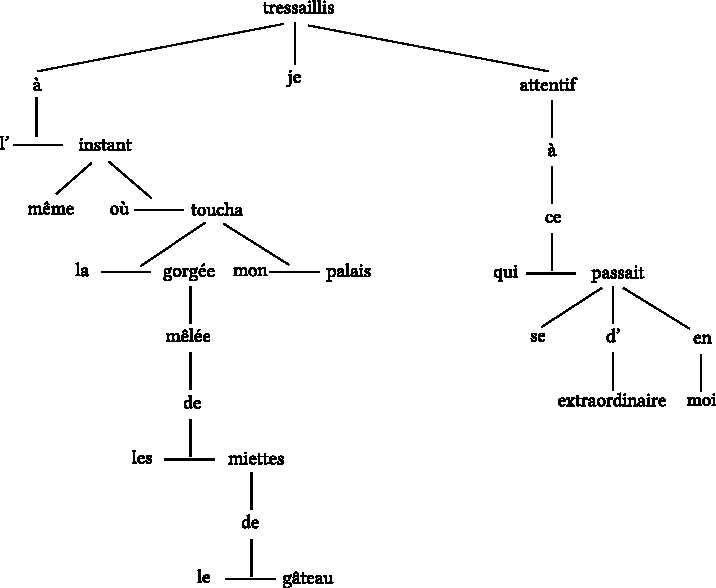
\includegraphics[scale=.9]{figures/polygraphs/poly-3.4.31.pdf}
    \caption{Structure de dépendance polygraphique\label{fig:proust}}
    \end{figure}
    
    Pour construire un arbre de constituants binaire, il faut décider dans quel ordre combiner chaque mot avec ses dépendants. Notons que lorsqu’une connexion n’est pas hiérarchisée, cette combinaison a lieu après les autres. Par exemple, si nous prenons la portion \textit{à l’instant même où la gorgée mêlée des miettes du gâteau toucha mon palais}, on obtient~la structure (ii), où le déterminant est le dernier élément à se combiner avec le nom :
    
    \begin{exe}
    \exi{(ii)}\relax
        [ \textit{à} ( \textit{l’} [ (\textit{instant même}) ( \textit{où} [ \textit{la} (\textit{gorgée} [\textit{mêlée des miettes du gâteau}] ) ] [ \textit{toucha} (\textit{mon palais}) ] ) ] ) ]
    \end{exe}
    Nous devons également décider dans quel ordre regrouper les trois dépendants de la tête de la phrase, \textit{tressaillis}. Dans ce cas, l’analyse standard regroupera probablement le sujet \textit{je} en premier, car les deux autres dépendants sont des éléments détachés prosodiquement. Concluons en rappelant que la stratification de la structure de constituants ne nous semble pas une question très pertinente. Nous pensons que le regroupement en constituants doit être fait à un autre niveau d’analyse en utilisant des critères de cohésion syntaxique. Ce sera l’objet du chapitre suivant.
 
 \corrigé{5} Le test de déplacement montre l’impossibilité de permuter les syntagmes en \textsc{à} et en \textsc{de} : *\textit{le train à Marseille de Paris}, *\textit{il travaille au vendredi du lundi}. Il semble donc qu’il ne s’agisse pas de deux groupes prépositionnels indépendants, lesquels peuvent généralement commuter (\textit{Elle parle de Marie à Zoé}, \textit{un timbre de ma collection à 10 euros}). Le test de clivage (voir la \sectref{sec:3.4.10} sur \textit{Les tests de constituance}) confirme cela : *\textit{c’est au vendredi qu’il travaille du lundi} vs *\textit{c’est du lundi qu’il travaille au vendredi} vs \textit{c’est du lundi au vendredi qu’il travaille}. Nous verrons dans le \chapfuturef{18} qu’on peut traiter cette construction comme une coordination.
}

\chapter{\gkchapter{La topologie}{Ordre des mots, linéarisation et regroupements}}\label{sec:3.5}

\section{La linéarité de la langue}\label{sec:3.5.0}

Une des caractéristiques de la langue est la \textstyleTermes{linéarité} de la chaîne parlée : les sons sont prononcés les uns à la suite des autres et il en va ainsi en général des unités de la langue et notamment des mots et des syntaxèmes. Les syntaxèmes, sauf rares exceptions (voir encadré ci-dessous), se suivent selon un \textstyleTermes{ordre linéaire}. (Un ordre linéaire est encore dit \textstyleTermes{total}, car \hi{tous les éléments sont ordonnés les uns par rapport aux autres}.)

La \textstyleTermes{place} qu’occupe chaque syntaxème dans l’ordre linéaire participe pleinement au sens de l’énoncé. Elle peut permettre de décider comment les unités sont combinées, et même si une combinaison est possible ou non. Par exemple, on peut envisager de placer les trois mots \textit{Marie}, \textit{Pierre} et \textit{poursuit} selon 6 ordres linéaires différents :

\ea\label{ex:poursuit}
\ea \textit{Marie poursuit Pierre}
\ex \textit{Pierre poursuit Marie}
\ex \textit{Pierre Marie poursuit}
\ex \textit{Marie Pierre poursuit}
\ex \textit{poursuit Marie Pierre}
\ex \textit{poursuit Pierre Marie}
\z
\z

Seules les combinaisons (\ref{ex:poursuit}a et b) portent des sens clairs en français. Et ces sens sont différents : les \hi{fonctions syntaxiques} de \textit{Marie} et \textit{Pierre}, sujet \textit{vs} objet du verbe \textsc{poursuivre}, et les rôles sémantiques qu’ils expriment, agent \textit{vs} patient du prédicat ‘poursuivre’, sont \hi{attribués en fonction de la place} des unités dans la phrase : l’élément devant le verbe est interprété comme sujet, celui après le verbe comme objet.

Les autres combinaisons ne sont pas nécessairement dépourvues de sens (si un étranger prononçait ces énoncés, on pourrait au moins comprendre qu’il s’agit d’une histoire de poursuite entre Pierre et Marie), mais elles ne respectent pas la syntaxe du français. Il est clair que la description précise d’une langue doit inclure les \hi{contraintes sur l’ordre} des syntaxèmes et sur la façon dont ils se regroupent. C’est ce que nous appelons la \textstyleTermes{topologie}, du grec \textit{topos}+\textit{logos} ‘étude des lieux’. Ce chapitre a comme but de proposer un modèle, appelé \textstyleTermes{modèle topologique} ou \textstyleTermes{interface syntaxe-topologie}, permettant d’exprimer facilement les différentes contraintes qui existent selon les langues dans la correspondance entre la structure syntaxique et la représentation qui exprime l’ordre linéaire et les regroupements linéaires, que nous appelons la \textstyleTermes{structure topologique}.

\loupe[sec:3.5.1]{Les exceptions à la segmentabilité}{%
    Nous venons d’insister sur la linéarité de la langue et le fait que les syntaxèmes sont essentiellement prononcés les uns à la suite des autres. On appelle cette dernière propriété la \textstyleTermesapprof{segmentabilité~}: la chaîne linéaire est segmentable en une succession d’unités élémentaires (voir la \sectref{sec:3.2.6} \textit{Structure syntaxique et structure topologique}).

    La segmentabilité possède un certain nombre d’exceptions.

    
    \tcbsubtitle{Prosodie} Malgré le caractère linéaire de la chaîne parlée, il est possible de jouer sur les différents paramètres du son pour communiquer deux informations simultanément. Ainsi, certains éléments de sens, comme par exemple les marqueurs d’interrogation ou de doute, ou la mise en avant de certains éléments de sens sont réalisés en utilisant la prosodie (l’intonation et le rythme – la mélodie de la phrase). Ces unités – les \textstyleTermesapprof{prosodèmes} – sont dites \textstyleTermesapprof{supra-segmentales}, car elles se superposent à la chaîne des unités segmentales que sont les phonèmes. À noter que la prosodie véhicule aussi, en plus de cela, des informations utiles pour le calcul des regroupements des unités linguistiques~et que les émotions du locuteur modifient également de manière significative la prosodie.
   
   \tcbsubtitle{Fusion} Dans les langues flexionnelles, certaines combinaisons de syntaxèmes \hi{fusionnent} en un unique morphe, tant et si bien qu’on ne peut plus discerner les signifiants des différents syntaxèmes et qu’il n’y a donc plus d’ordre entre eux (voir la \sectref{sec:2.2.22} sur \textit{Amalgame, alternance et mégamorphe}). Il existe aussi des syntaxèmes qui s’enchevêtrent, comme dans la conjugaison des langues sémitiques, où les lexèmes verbaux sont réalisés par des consonnes et la flexion par des voyelles intercalées (voir l’\encadref{sec:3.1.15} sur les \textit{Syntaxèmes discontinus}). Pour une typologie des différents cas de non-segmentabilité des syntaxèmes flexionnels, voir l’encadré sur les \textit{Langues isolantes, agglutinantes et flexionnelles} du \chapfuturef{14}).
    
    \tcbsubtitle{Phrasèmes} Si les syntaxèmes sont globalement continus (à l’exception des situations rappelées ci-dessus), ce n’est pas le cas des sémantèmes. Les phrasèmes peuvent être réalisés par des configurations de syntaxèmes qui ne se placeront pas nécessairement les uns à côté des autres : \textit{il ne} \textbf{\textit{bris}}\textit{a pas immédiatement} \textbf{\textit{la glace}}, «~\textit{Fais pas} \textbf{\textit{ci}}, \textit{fais pas} \textbf{\textit{ça~}}!~». Il faut néanmoins remarquer que la réalisation de sémantèmes discontinus passe presque uniquement par le recours à des constructions syntaxiques qui sont utilisées par ailleurs pour réaliser des combinaisons libres de syntaxèmes et qui s’appliquent aux différentes composantes du sémantème (voir le \chapref{sec:2.3}).
    
    \tcbsubtitle{Langues des signes} Il est important de souligner que les contraintes sur la linéarité sont l’apanage des \hi{langues vocales} (c’est-à-dire utilisant la voix comme canal de communication) et de leurs contreparties écrites. Les \hi{langues des signes}, réalisées par des gestes dans l’espace à trois dimensions, échappent en partie à la contrainte de linéarité. Il est possible en réalisant le signe associé à un sens donné (‘chien’, ‘voiture’, ‘maison’, ‘maladie’, etc.) de produire en même temps toutes sortes de modifieurs en adaptant la réalisation du geste : un chien agressif ou au contraire affectueux, une voiture rapide ou aux mouvements chaotiques, une grande maison, etc. Cette particularité des langues des signes par rapport aux langues vocales est généralement appelée l’\textstyleTermesapprof{iconicité} : il s’agit de la possibilité de réaliser des signes iconiques, c’est-à-dire qui ont une ressemblance avec l’objet qu’il dénote. Même sans utiliser l’iconicité, la réalisation d’un signe verbal comme ‘demander’ (réalisé en joignant les mains à plat en langue des signe française) indiquera en fonction de l’orientation du geste (vers le locuteur, l’interlocuteur ou un autre point de l’espace) qui demande à qui, sans qu’il soit nécessaire d’ajouter des pronoms. La diathèse du lexème est donc réalisée en même temps que le lexème. C’est bien la réalisation du signal dans un espace tridimensionnel qui permet de cumuler autant d’informations en un seul geste.
}
\section{Ordre des mots \textit{vs} topologie}\label{sec:3.5.2}

On renvoie traditionnellement à la branche de la syntaxe qui s’intéresse aux questions d’ordre en parlant d’\textstyleTermes{ordre des mots}. Nous préférons parler de \textstyleTermes{topologie} et cela pour au moins trois raisons.

Premièrement, nous considérons que les unités minimales de la syntaxe sont les syntaxèmes et non les mots et donc que les questions d’ordre commencent avec l’ordre des syntaxèmes à l’intérieur des mots.

Deuxièmement, nous ne nous intéressons pas seulement à l’ordre relatif des syntaxèmes (ou des mots ou des unités syntaxiques en général), mais plus généralement à la \textstyleTermes{position} qu’occupent ces éléments dans une structure qui est plus riche qu’un simple ordre linéaire. C’est ce que désigne la topologie, qui est l’étude des lieux ou places (du grec \textit{topos} ‘lieu’).

Troisièmement, le terme \textit{topologie} (du grec \textit{logos} ‘étude’), à la différence de \textit{ordre des mots}, renvoie clairement à un domaine d’étude de la langue ; il permet de plus de dériver l’adjectif \textit{topologique} et de parler par exemple de \textit{structure topologique}, de \textit{constituant topologique} ou de \textit{niveau topologique}.

Le terme \textit{topologie} provient de la tradition grammaticale allemande, où le ter\-me est d’usage depuis le milieu du 20\textsuperscript{e} siècle (voir l'\encadref{sec:3.5.38} sur \textit{l’Historique de la description topologique}). Les mathématiques ont également un sous-domaine nommé \textit{topologie}, qui s'intéresse aussi lui aussi à la façon dont les éléments se placent les uns par rapport aux autres dans des ensembles munis d’une structure, mais sans rapport direct avec la topologie linguistique.

\section{Place linéaire et position syntaxique}\label{sec:3.5.3}

Toute unité linguistique (phonologique, morphologique, syntaxique ou sémantique) émise en contexte, dès qu’elle est segmentable, a une place dans l’ordre linéaire. Dans tout cet ouvrage, nous opposons les termes \textstyleTermes{place (linéaire)} et \textstyleTermes{position (structurelle)} : \textit{place} est toujours associé à un lieu dans l’ordre linéaire, tandis que \textit{position} est associé à un lieu dans une structure plus complexe. On peut penser, comme moyen mnémotechnique, à une personne assise sur une chaise : cette personne peut changer de position sans changer de place. Les syntaxèmes sont comme des personnes assises sur des chaises les unes à la suite des autres : chacun à une place sur une chaise et peut adopter une position particulière en s'adressant à son voisin de gauche ou de droite ou à quelqu'un de plus éloigné ; il peut changer de position en restant à la même place (on parlera d’\textstyleTermes{ambiguïté syntaxique}) ou changer de place en gardant la même position (on parlera d’\textstyleTermes{ordre libre}).

Nous avons défini aux chapitres précédents la structure syntaxique. La position d’un élément dans la structure syntaxique est appelée sa \textstyleTermes{position syntaxique}. La syntaxe s’intéresse aux combinaisons libres (voir la \sectref{sec:3.1.6} sur \textit{Syntaxe et morphologie}) et la position syntaxique d’un élément indique donc avec quoi il se combine, sans référence à l’ordre linéaire. Deux éléments occupent la même position syntaxique s’ils jouent un rôle similaire et s’excluent mutuellement. Ainsi dans les trois phrases de \REF{ex:quila} ,les unités  \textit{Marie}, \textit{la} et \textit{qui} occupent la même position syntaxique, car elles correspondent toutes à la personne que Pierre regarde et elles \textit{s’excluent} \textit{mutuellement}, comme le montre \REF{ex:quilapas}


\ea\label{ex:quila}
  \ea \textit{{Pierre regarde} \textbf{{Marie}}.}
  \ex \textit{{Pierre} \textbf{{la}}  {regarde.}}
  \ex \textit{\textbf{{Qui}}  {Pierre regarde-t-il} ?}
  \z
\z

\ea\label{ex:quilapas}
\ea[*]{\textit{{Pierre} \textbf{{la}}  {regarde} \textbf{{Marie}}.}}
\ex[*]{\textit{\textbf{Qui}  {Pierre} \textbf{{la}} \textit{regarde-t-il} ?}}
\ex[*]{\textit{\textbf{Qui}  {Pierre regarde-t-il} \textbf{{Marie}} ?}}
\z
\z

Cette impossibilité pour les unités \textit{Marie, la} et \textit{qui} de cooccurrer implique qu’elles \hi{occupent une même position à un certain niveau structurel}, et cela alors qu’elles n’occupent pas la même place. Ceci nous permet de conclure que la place linéaire et la position syntaxique sont bien deux notions distinctes.

\section{Position topologique}\label{sec:3.5.4}

Nous venons de voir que des éléments occupant la même position syntaxique pouvaient être à des places linéaires différentes. À l’inverse, des éléments de positions syntaxiques différentes peuvent venir occuper la même place linéaire.

Par exemple, en français, le sujet du verbe se place généralement devant le verbe, comme en (\ref{ex:guirlandes}a), mais il est parfois possible que le sujet se place après le verbe, notamment lorsqu’un complément locatif est placé devant le verbe, comme en (\ref{ex:guirlandes}b).

\ea\label{ex:guirlandes}
    \ea\textit{\textbf{{Des guirlandes}}  {pendaient au plafond}.}
    \ex\textit{\textbf{{Au plafond}}  {pendaient des guirlandes}.}
\z
\z

On peut ici considérer que le complément locatif vient occuper la place qu’occupe usuellement le sujet, puisqu’il n’est pas possible que le sujet se place après le verbe si le locatif ne vient pas devant le verbe :

\ea
\ea[\textsuperscript{??}]{\textit{Pendaient au plafond des guirlandes.}}
\ex[\textsuperscript{?}*]{\textit{Pendaient des guirlandes au plafond.}}
\z
\z

Par ailleurs, lorsque le locatif et le sujet sont tous les deux devant le verbe, le locatif est obligatoirement dans une position détachée, avec un contour prosodique particulier, sanctionné à l’écrit par une virgule :

\ea \textit{Au plafond, des guirlandes pendaient.} \z

Lorsque le locatif est entre le sujet et le verbe, il est immédiatement interprété comme faisant partie du sujet :

\ea[\textsuperscript{\#}]{\itshape Des guirlandes au plafond pendaient.}\z

Cette exclusion mutuelle dans un lieu de l’ordre linéaire laisse supposer qu’un tel lieu est plus qu’une simple place, qu’il y a de la structure qui est en jeu. Cette structure, nous l’appellerons la \textstyleTermes{structure topologique} et un lieu de cette structure, comme celui où \textit{des guirlandes} et \textit{au plafond} commutent devant le verbe, sera appelé une \textstyleTermes{position topologique}. On peut ainsi reformuler ce que nous venons de dire concernant le sujet et le complément locatif : en français, il existe devant le verbe fini une position topologique qui accueille en général le sujet, mais qui peut être aussi remplie par un complément locatif, le sujet allant dans ce cas dans une autre position topologique.

\globe[sec:3.5.5]{Le cas des langues V2}{%
    Il existe différentes langues, dites \textstyleTermes{V2}, où la tête de la phrase, généralement un verbe, occupe nécessairement la \hi{deuxième place}. Autrement dit, il existe devant le verbe une unique position topologique qui doit être remplie par une et une seule unité syntaxique. Tel est le cas des langues germaniques.

    Contrairement au français, où toute phrase peut contenir un nombre quelconque de compléments circonstanciels antéposés au verbe, l’allemand contraint toute phrase déclarative à avoir un unique constituant devant le verbe. Et contrairement au français, ce constituant n’a pas plus à être le sujet que n’importe quel autre dépendant du verbe. Ainsi la phrase française \textit{Malheureusement, Peter se crotte encore le nez} permet-elle des traductions à ordres variés. Parmi elles :
    
    \ea \label{ex:Nase1}
    \ea \gll   Peter popelt leider {mal wieder}  in seiner Nase.\\
                Peter   creuse   malheureusement {une fois de plus}   dans son nez.\\
    \ex     \textit{Leider       popelt   Peter   mal wieder  in seiner Nase.}
    \ex     \textit{Mal wieder   popelt   leider   Peter    in seiner Nase.}
    \ex     \textit{In seiner Nase   popelt   leider   mal wieder   Peter.}
    \z
    \z
   
    Par contre, une traduction qui suivrait le même ordre des mots que la phrase française initiale serait agrammaticale :
    
    \ea[*]{\itshape Leider Peter popelt mal wieder in seiner Nase.}\z
    Ceci parce que \textit{leider} ‘malheureusement’ et \textit{Peter} ne forment pas ensemble un seul constituant. Ce constituant initial de toute phrase déclarative de l’allemand est dit occuper le \textstyleTermesapprof{champ initial} (ou \textit{Vorfeld} ‘pré-champ’). Le verbe fini juste après est dit être en position \textstyleTermesapprof{V2}. 
    
    Le champ initial (mis entre crochets dans les exemples suivants) peut être occupé par un seul constituant quelle que soit sa complexité, y compris un participe passé comme dans les exemples suivants :

    \ea\label{ex:Nase-participe}
    \ea
    \gll [In seiner Nase gepopelt]   hat leider {mal wieder} Peter.\\
         {\db}Dans son nez creusé   a   malheureusement   {une fois de plus}   Peter.\\
    \glt   ‘Peter s’est malheureusement à nouveau crotté le nez.’
    \ex
    \gll [Vor allen {mal wieder} in seiner Nase zu popeln gewagt] hat leider Peter.\\
     {\db}Devant tous {une fois de plus} dans son nez de creuser osé   a   malheureusement   Peter.\\
    \glt   ‘Peter a malheureusement {une fois de plus}  osé se crotter le nez devant tout le monde.’
    \z
    \z

Nous présenterons plus en détail la modélisation de l'ordre des mots en allemand dans l'\encadref{sec:3.5.36} sur \textit{La structure topologique de l'allemand}.

    Comme nous l’avons montré dans la \sectref{sec:3.5.4} qui précède, le français possède aussi une forme de syntaxe V2 avec une position devant le verbe qui doit être occupée soit par le sujet, soit par un complément locatif en cas d’inversion du sujet. De ce point de vue, le français conserve des traces d’une syntaxe germanique héritée de l’époque où le latin a évolué en roman, puis en ancien français par l’intégration de peuples germaniques dans l’espace latinophone. Lorsqu’un groupe important de locuteurs non natifs est contraint de parler une nouvelle langue (ici le latin), il en adopte le lexique, tout en conservant partiellement la syntaxe de sa langue d’origine (ici des langues germaniques, et notamment le francique, la langue des Francs).

    On retrouve des restes de ce caractère V2 en anglais, qui est aussi une langue d’origine germanique (voir l’exercice 7 sur la topologie de l’anglais). Les langues germaniques ne sont pas les seules langues V2 de par le monde : on peut mentionner par exemple le breton, une langue celtique, ou le wolof, une langue Niger-Congo parlée au Sénégal. Le serbe, une langue slave, possède un phénomène comparable avec un amas de clitiques qui vient se placer en deuxième position.
}
\section{Linéarisation}\label{sec:3.5.6}
\begin{sloppypar}
Il est important de souligner que nous concevons l’ordre des syntaxèmes comme le résultat d’un processus nécessaire dans l’expression du sens. Le sens n’est pas linéaire a priori (ni même hiérarchisé, voir la \sectref{sec:1.2.9} sur la \textit{Structure hiérarchique}), mais l’usage du canal vocal oblige à un encodage linéaire de l’information. La question de l’ordre des syntaxèmes est donc vue comme un processus de \textstyleTermes{linéarisation} de l’information.
\end{sloppypar}

La linéarisation est modélisée comme une correspondance entre deux structures de niveaux différents : une structure hiérarchique non ordonnée – la structure syntaxique (voir le \chapref{sec:3.3}) – et une structure ordonnée. Cette idée est centrale dans les \textit{Éléments de syntaxe structurale} de Lucien \citet{tesniere1959elements}, qui distingue l’\hi{ordre structural} et de l’\hi{ordre linéaire}. On trouve déjà chez Claude \citet{buffier1709grammaire} la distinction entre syntaxe et style, puis chez Dumarsais entre syntaxe et construction. Voici ce que ce dernier en dit dans l’article «~Construction~» de l’\textit{Encyclopédie} :

\begin{quote}
    «~Je crois qu’on ne doit pas confondre \textit{construction} avec \textit{syntaxe}. Construction ne présente que l’idée de combinaison et d’arrangement. Cicéron a dit selon trois combinaisons différentes, \textit{accepi litteras tuas, tuas accepi litteras}, et \textit{litteras accepi tuas} : il y a là trois \textit{constructions}, puisqu’il y a trois différents arrangements de mots ; cependant il n’y a qu’une syntaxe ; car dans chacune de ces constructions il y a les mêmes signes des rapports que les mots ont entre eux, ainsi ces rapports sont les mêmes dans chacune de ces phrases.~» (\citealt{Dumarsais1754} : 72)
\end{quote}

Nous allons étudier la question de la linéarisation de la structure syntaxique dans la suite de ce chapitre. Nous défendons l'idée que cette étape de linéarisation ne consiste pas seulement à ordonner les unités syntaxiques, syntaxèmes et autres, mais qu'elle induit une structure, avec un emboîtement de constituants, que nous appelons les \textstyleTermes{constituants topologiques}. Ceux-ci jouent un rôle dans la linéarisation et le calcul de l'ordre des mots, mais aussi dans le calcul de la prosodie (voir l’\encadref{sec:3.5.35} sur \textit{Topologie et prosodie}).

La partie de la grammaire qui assure la correspondance entre la structure syntaxique et la structure topologique, et donc en particulier la linéarisation, s’appelle le \textstyleTermes{modèle topologique}. Dans la suite, nous allons présenter le cadre général de la construction d’un modèle topologique et nous construirons notamment les modèles topologiques du français et de l’allemand.

\loupe[sec:3.5.7]{Une représentation syntaxique non ordonnée ?}{%
    La linéarisation est une étape dans le processus de synthèse d’un énoncé à partir d’un sens (voir l'\encadref{sec:1.1.1} sur \textit{La langue comme correspondance sens-texte} et le \chapref{sec:1.2} sur la \textit{Production d’un énoncé}). Nous pensons que l’information à communiquer par un locuteur, qui va constituer le sens de son message, n’est pas linéarisée, ni même hiérarchisée a priori. C’est le processus de communication qui oblige à linéariser. La \textstyleTermesapprof{structure communicative}, qui encode la façon dont l’information est structurée pour être communiquée (voir l’\encadref{sec:1.2.4} sur \textit{Les composantes du sens}), joue ainsi dans de nombreuses langues un rôle primordial dans l’ordre des syntaxèmes (voir l’\encadref{sec:3.5.24} sur l’\textit{Ordre communicativement dirigé}).

    Nous considérons que la structure communicative fait partie de la représentation du sens à communiquer et ceci quelle que soit la langue, alors que l’ordre linéaire, qui en découle parfois directement, ne fait pas lui-même partie du sens. En procédant ainsi, nous pouvons nous abstraire des idiosyncrasies d’une langue particulière et nous rapprocher d’une représentation du sens plus universelle. Une telle représentation permet alors de modéliser la traduction ou le paraphrasage (qui est une traduction intra-langue) : en effet, des traductions ou paraphrases peuvent partager le même sens et des structures communicatives similaires, tout en ayant des ordres linéaires très différents (voir l’\encadref{sec:3.5.13} sur l’\textit{Ordre dominant}).

    Même si l’on admet que le sens est non ordonné, on est en droit de se demander pourquoi nous considérons une \hi{représentation syntaxique non ordonnée} (l’arbre de dépendance) entre le sens et l’ordre linéaire.

    Premièrement, on a vu qu’il est possible de définir une structure hiérarchique qui rende compte de propriétés importantes de l’énoncé sur la combinaison des unités entre elles (voir le \chapref{sec:3.2}) et de considérer cette structure indépendamment de l’ordre linéaire. 

    Deuxièmement, il y a de bonnes raisons de penser que la structure hiérarchique est bien un intermédiaire entre le sens et l’ordre linéaire. Avant tout parce que le sens est multidimensionnel, la structure hiérarchique bidimensionnel et l’ordre linéaire unidimensionnel (voir l'\encadref{sec:1.2.10} \textit{Du sens au texte : de 3D à 1D}).
    Pour cette raison, nous pensons qu'il est plus simple de modéliser le passage d'une structure sémantique à une structure linéairement ordonnée en procédant en deux étape : le passage du sens à une structure hiérarchique, déjà évoquée au \chapref{sec:1.2} et étudiée en détail au \chapref{sec:13} et le passage de cette strycture hiérarchique à un ordre linéaire étudiée ici et formalisée dans la suite de ce chapitre. Il serait beaucoup moins simple de passer directement du sens à un ordre linéaire.

    Cette dernière affirmation doit quand même être modulée : dans le processus de synthèse d’un texte à partir d’un sens, l’ordre linéaire semble parfois prévaloir sur la structure hiérarchique. On a notamment cette impression lorsqu’on compare des constructions de français oral avec des constructions plus écrites, comme dans ces exemples classiques :

    \ea\label{ex:guidon}
    \ea  \textit{Moi, mon frère, son vélo, le guidon, il est cassé.}
    \ex  \textit{Le guidon du vélo de mon frère est cassé.}
    \z
    \z
    Comme on le voit dans l'énoncé (\ref{ex:guidon}a), le plus oral des deux, chaque élément de sens forme un îlot rectionnel indépendant et cet énoncé échappe ainsi à une structure hiérarchique complète, à l’inverse de l'énoncé (\ref{ex:guidon}b). On est en droit de se demander si dans ce premier énoncé, la structure communicative n’a pas d’abord permis de construire une structure topologique avec des places qu’on est ensuite venu remplir avec de petits segments organisés hiérarchiquement. Cela ne remet toutefois pas en cause la possibilité de considérer la structure linéaire et la structure hiérarchique indépendamment l’une de l’autre.

    Dire que l’on peut considérer ces deux structures indépendamment l’une de l’autre ne signifie absolument pas qu’elles soient indépendantes l’une de l’autre. Bien au contraire, elles se contraignent l’une l’autre par un ensemble de propriétés qui constituent les règles du modèle topologique. Dans la suite, nous allons donc nous intéresser au «~produit~» de ces deux structures, l’arbre de dépendance ordonné.
}
\pagebreak\largerpage
\loupe[sec:3.5.8]{Mouvement et ordre de base}{%
    Notre conception de l’ordre des syntaxèmes s’oppose à une autre conception, celle de la grammaire générative, développée autour de Noam Chomsky depuis la fin des années 1950. Dans cette conception, une unique structure syntaxique de base \hi{ordonnée} est postulée pour chaque construction de chaque langue. Les différents ordres observés sont obtenus par des \textstyleTermesapprof{mouvements} au sein de la structure syntaxique de base.

    La notion de mouvement repose sur l’idée que tout changement de place linéaire est aussi un changement de position syntaxique. Nous distinguons pour notre part position topologique et position syntaxique : à chaque position syntaxique correspondent au moins autant de positions topologiques qu’il y a de placements possibles. Que l’on considère \textit{le livre que} \textbf{\textit{Zoé lit}} ou \textit{le livre que}\textbf{ \textit{lit} \textit{Zoé}}, le nom \textit{Zoé} occupe toujours la même position syntaxique de sujet de la forme verbale \textit{lit} ; seule sa position topologique change. Autrement dit, à partir de la structure syntaxique commune à ces deux syntagmes, on aura deux linéarisations possibles.

    Nous renvoyons également à l’\encadref{sec:3.2.7} \textit{De la non-séparation des ordres aux mouvements}, où nous montrons que l’introduction du mouvement dans un modèle linguistique est une conséquence immédiate de la non-distinction de la position syntaxique et de la place linéaire, caractéristique des modèles générativistes. Dans ces modèles, il est supposé que toute construction possède un \hi{ordre de base}. Ainsi en français, l’ordre de base entre le verbe et son sujet est l’ordre sujet-verbe (\textbf{\textit{Zoé lit}} \textit{un livre}). Lorsque le sujet est après le verbe (\textit{le livre que} \textbf{\textit{lit Zoé}}), on parle traditionnellement de \hi{sujet inversé}. C’est une terminologie traditionnelle, mais problématique, car elle suggère qu’il y a une opération d\hi{’inversion} (\textit{le livre que Zoé lit} \textrm{→} \textit{le livre que lit Zoé}) à partir de l’ordre de base.

    Nous rejetons pour notre part la notion d’ordre de base. Nous considérons qu’il y a un processus de linéarisation qui permet de calculer à partir d’une structure syntaxique non ordonnée différents ordres possibles. Il est bien sûr possible qu’un des ordres soit \hi{privilégié}, voire \hi{obligatoire}, et nous parlerons alors d’\textstyleTermesapprof{ordre dominant} (voir l'\encadref{sec:3.5.13} sur l’\textit{Ordre dominant} et l'\encadref{sec:3.5.23} sur \textit{Les langues dites à ordre libre}). L’ordre dominant est un \hi{ordre par défaut}, généralement peu marqué communicativement, mais qui ne sert en aucun cas de base au calcul des autres ordres possibles.

    L’idée d’un ordre de base et la notion d’inversion par rapport à l’ordre de base remonte au moins au 18\textsuperscript{e} siècle. L’article «~Inversion~» de l’\textit{Encyclopédie} écrit par Nicolas Beauzée et publié en \citeyear{Beauzée1765} s’inscrit parfaitement dans son temps en faisant référence à un ordre analytique supposé l’ordre naturel de la pensée et donc universel : 
    \begin{quote}«~C’est l’ordinaire dans toutes ces langues que le sujet précède le verbe, parce qu’il est dans l’ordre que l’esprit voie d’abord un être avant qu’il en observe la manière d’être ; que le verbe soit suivi de son complément, parce que toute action doit commencer avant que d’arriver à son terme ; que la préposition ait de même son complément après elle, parce qu’elle exprime de même un sens commencé que le complément achève.~»
    \end{quote}
    Voir également, dans l’\encadref{sec:3.5.24} \textit{Ordre communicativement dirigé,} la distinction entre langues analogues et langues transpositives introduite par \citet{girard1747vrais}. 
    
    Néanmoins, à cette époque déjà, le débat est vif et d’autres linguistes ont une approche beaucoup plus nuancée, comme Dumarsais, qui dans l’article «~Construction~» de l’\textit{Encyclopédie} publié en \citeyear{Dumarsais1754}, souligne que, s’il peut y avoir un ordre dominant, celui-ci est avant tout acquis : 
    \begin{quote}
   «~La construction simple est aussi appelée construction naturelle, parce que c’est celle que nous avons apprise sans maître, par la seule constitution mécanique de nos organes, par notre attention et notre penchant à l’imitation. […] Telle est la relation établie entre la pensée et les mots, c’est-à-dire, entre la chose et les signes qui la font connaître : connaissance acquise dès les premières années de la vie, par des actes si souvent répétés, qu’il en résulte une habitude que nous regardons comme un effet naturel.~»
    \end{quote}
}
\section{Arbre de dépendance ordonné}\label{sec:3.5.9}

Nous avons vu au \chapref{sec:3.3} comment représenter la structure syntaxique à l’aide d’un arbre de dépendance. Nous envisageons la linéarisation comme la correspondance entre un arbre de dépendance (non ordonné) et un ordre linéaire. 

\Definition{\textstyleTermesapprof{arbre de dépendance ordonné}}{
La structure combinant un arbre de dépendance et un ordre linéaire sur les nœuds de cet arbre est appelé un \textstyleTermesapprof{arbre de dépendance ordonné}.
}

Si nous reprenons l’exemple des chapitres précédents (\textit{Beaucoup de gens aimeraient passer Noël en Laponie}), nous devons mettre en correspondance les deux structures de la figure~\ref{fig:noel-double}, où l’ordre linéaire est représentée par la relation de précédence qui unit les nœuds successifs (sur le lien entre la relation d’ordre et la relation de précédence, on pourra consulter l’\encadref{sec:3.3.30} sur \textit{Dépendance, dominance et transitivité}).


\begin{figure}
\begin{tikzpicture}
    \begin{scope}[every node/.style={CircleNode},level distance=2\baselineskip,
                  level 1/.style={sibling distance=30mm},
                  level 2/.style={sibling distance=15mm},
                  level 3/.style={sibling distance=10mm}
                  ]
      \node (root) {}
        child { node{} child { node{} child { node{} } } }
        child { node{} child { node{} } 
                       child { node{} 
                            child { node{} }
                       }
              };
    \end{scope}
    \begin{scope}[every node/.style={font=\itshape\strut}]
    \node [above=1pt of root] {aimeraient};
    \node [left=1pt of root-1] {beaucoup};
    \node [left=1pt of root-1-1] {de};
    \node [left=1pt of root-1-1-1] {gens};
    \node [right=1pt of root-2] {passer};
    \node [left=1pt of root-2-1] {Noël};
    \node [right=1pt of root-2-2] {en};
    \node [right=1pt of root-2-2-1] {Laponie};
    \end{scope}
\end{tikzpicture}\bigskip\\
\begin{tikzpicture}
\begin{scope}[every node/.style={CircleNode},grow=right]
\node (root) {} child { node {} child { node{} child { node{} child { node{}  
                    child { node{} child { node{} child { node{} } } } } } } }; 
\end{scope}
\foreach \pos/\text in {/beaucoup, -1/de, -1-1/gens, -1-1-1/aimeraient, -1-1-1-1/passer,
                        -1-1-1-1-1/Noël, -1-1-1-1-1-1/en, -1-1-1-1-1-1-1/Laponie} 
      {\node [font={\itshape\strut}, below=1pt of root\pos] {\text};}
\end{tikzpicture}
\caption{\label{fig:noel-double}Arbre de dépendance et ordre linéaire}
\end{figure}


On peut représenter la correspondance entre les deux structures, l’arbre de dépendance et l’ordre linéaire, en alignant les nœuds qui se correspondent deux à deux, comme dans la figure~\ref{fig:noel-Lecerf}. Cette représentation qui apparaît dans les travaux d'Yves \citet{lecerf1960programme}, sera appelée l'\textstyleTermesapprof{arbre de dépendance projeté} ou la  \textstyleTermesapprof{représentation à la Lecerf} de l'arbre de dépendance ordonné. Dans cette représentation, les deux structures en correspondance sont bien séparées et la correspondance est représentée de manière explicite par des lignes verticales (en pointillée), que Lecerf appelle des \textstyleTermesapprof{projetantes}.

\begin{figure}
\begin{tikzpicture}
\begin{scope}[every node/.style={CircleNode},grow=right]
\node (root) {} child { node {} child { node{} child { node{} child { node{}  
                    child { node{} child { node{} child { node{} } } } } } } }; 
\end{scope}
\foreach \pos/\text/\distance/\place in 
            {
             /beaucoup/6/above, 
             -1/de/4/above, 
             -1-1/gens/2/above, 
             -1-1-1/aimeraient/8/above, 
             -1-1-1-1/passer/6/above,
             -1-1-1-1-1/Noël/4/below left, 
             -1-1-1-1-1-1/en/4/above, 
             -1-1-1-1-1-1-1/Laponie/2/above
            } 
      {
        \node [ font={\itshape\strut}, below=1pt of root\pos ] {\text};
        \node [
                above=\distance\baselineskip of root\pos,
                label=\place:{\itshape\strut\text},
                CircleNode
              ] (\text) {};
        \draw [ dashed ] (\text) -- (root\pos);
      }
      \begin{scope}[on background layer]
        \draw (aimeraient) -- (beaucoup) -- (de) -- (gens);
        \draw (aimeraient) -- (passer) -- (Noël); 
        \draw (passer) -- (en) -- (Laponie);
      \end{scope}
\end{tikzpicture}
\caption{Arbre de dépendance projeté ou représentation à la Lecerf d'un arbre de dépendance ordonné\label{fig:noel-Lecerf}}

\end{figure}

L’ordre linéaire et l’arbre de dépendance sont en fait deux structures sur \hi{un même ensemble} d’éléments.  Une structure combinant ainsi deux structures est appelée une \textstyleTermesapprof{structure produit} en mathématique.
Une représentation de la structure produit que forment ensemble l’ordre linéaire et l’arbre de dépendance est donnée dans la figure~\ref{fig:noel-Hudson}. Dans cette représentation, introduite par Richard \citet{hudson1984word}, toutes les dépendances sont représentées dans le même demi-plan au-dessus de la ligne formée par la chaîne linéaire. Une dépendance verticale (sans gouverneur) vient en plus marquer la position de la racine de l'arbre de dépendance. L’intérêt de cette dépendance apparaîtra clairement lorsque nous parlerons de projectivité (\sectref{sec:3.5.14} sur \textit{Projectivité et dépendances projectives}). Nous appellerons cette représentation l'\textstyleTermesapprof{arbre de dépendance en ligne} ou la  \textstyleTermesapprof{représentation à la Hudson} d'un arbre de dépendance ordonné.

\vfill
\begin{figure}[H]
\begin{tikzpicture}
\begin{scope}[every node/.style={CircleNode},grow=right]
\node (root) {} child { node {} child { node{} child { node{} child { node{}  
                    child { node{} child { node{} child { node{} } } } } } } }; 
\end{scope}
\foreach \pos/\text in {/beaucoup, -1/de, -1-1/gens, -1-1-1/aimeraient, -1-1-1-1/passer,
                        -1-1-1-1-1/Noël, -1-1-1-1-1-1/en, -1-1-1-1-1-1-1/Laponie} 
      {\node [font={\itshape\strut}, below=1pt of root\pos] {\text};}
      
\path (root) edge[bend left,-{Triangle[]}] (root-1)
      (root-1) edge[bend left,-{Triangle[]}] (root-1-1)
      (root-1-1-1) edge[bend right,-{Triangle[]},out=315,in=225] (root)
                   edge[bend left,-{Triangle[]}] (root-1-1-1-1)
      (root-1-1-1-1) edge[bend left,-{Triangle[]}] (root-1-1-1-1-1)
                     edge[bend left,-{Triangle[]},out=60,in=120] (root-1-1-1-1-1-1)
      (root-1-1-1-1-1-1) edge[bend left,-{Triangle[]}] (root-1-1-1-1-1-1-1);

\draw[{Triangle[]}-] (root-1-1-1) -- ++(0,1cm);
\end{tikzpicture}
\caption{Arbre de dépendance en ligne ou représentation à la Hudson d'un arbre de dépendance ordonné\label{fig:noel-Hudson}}
\end{figure}
\vfill
\pagebreak



\loupe[sec:3.5.10]{Format tabulaire et treebanks}{%
    Un arbre de dépendance ordonné peut être encodé dans un \textstyleTermesapprof{format tabulaire} comme dans la table~\ref{tab:conll}.
    
    \begin{table}[H]
    \caption{Encodage tabulaire d'un arbre de dépendance ordonné\label{tab:conll}}
    \begin{tabular}{cllcl}
    \lsptoprule
    Identifiant & Mot & Catégorie & Gouverneur & Fonction\\
    \midrule
    1 & Beaucoup & Adverbe & 4 & sujet\\
    2 & de & Préposition & 1 & complément\\
    3 & gens & Nom & 2 & complément\\
    4 & aimeraient & Verbe & 0 & racine\\
    5 & passer & Verbe & 4 & objet\\
    6 & Noël & Nom & 5 & objet\\
    7 & en & Préposition & 5 & complément\\
    8 & Laponie & Nom & 7 & complément\\
    \lspbottomrule
    \end{tabular}
    \end{table}

    Ce tableau a 5 colonnes. La deuxième contient les mots de la phrase dans l’ordre. Pour chacun de ces mots, on peut donner autant d’informations qu’on veut : ici on donne leur catégorie syntaxique dans la troisième colonne. La première colonne attribue un identifiant à chaque mot. Grâce à cet identifiant, on peut faire référence à n’importe quel mot de la même phrase. Ainsi dans la quatrième colonne, on indique pour chaque mot quel est son gouverneur. On peut ensuite ajouter des informations sur cette relation : la dernière colonne indique la fonction syntaxique que remplit chaque mot par rapport à son gouverneur.

    Le tableau se lit donc ainsi : le mot 5 est \textit{passer}. Ce mot est un verbe qui a pour gouverneur le mot 4 dont il est l’objet. Le mot 4 est \textit{aimeraient}. Ce verbe est la racine de l’arbre de dépendance. Il n’a donc pas de gouverneur, ce qu'on indique par un identifiant 0 dans la colonne du gouverneur.

    On peut représenter l’information contenue dans la table~\ref{tab:conll} par la structure étiquetée de la figure~\ref{fig:noel-conll}.

    \begin{figure}[H]
    \small
    \caption{Arbre de dépendance ordonné étiqueté\label{fig:noel-conll}}
    \begin{tikzpicture}[scale=0.925]
        \begin{scope}[every node/.style={CircleNode},grow=right]
        \node (root) {} child { node {} child { node{} child { node{} child { node{}  
                            child { node{} child { node{} child { node{} } } } } } } }; 
        \end{scope}
        \foreach \pos/\text/\i/\type in {
                    /beaucoup/1/Adverbe,
                    -1/de/2/Prép,
                    -1-1/gens/3/Nom,
                    -1-1-1/aimeraient/4/Verbe,
                    -1-1-1-1/passer/5/Verbe,
                    -1-1-1-1-1/Noël/6/Nom, 
                    -1-1-1-1-1-1/en/7/Prép, 
                    -1-1-1-1-1-1-1/Laponie/8/Nom
                } 
            {\node [font={\strut}, align=center, below=1pt of root\pos] (\text) {\i\\\itshape\text\\\type};}
        
        \begin{scope}[>={Triangle[]},every node/.style={above,midway,font=\footnotesize}]
        \path (root) edge[bend left,->] node  {comp} (root-1)
            (root-1) edge[bend left,->] node  {comp} (root-1-1)
            (root-1-1-1) edge[bend right,->,out=285,in=255] node  {sujet} (root)
                        edge[bend left,->] node  {objet} (root-1-1-1-1)
            (root-1-1-1-1) edge[bend left,->] node  {objet} (root-1-1-1-1-1)
                            edge[bend left,->,out=75,in=105] node  {comp} (root-1-1-1-1-1-1)
            (root-1-1-1-1-1-1) edge[bend left,->] node  {comp} (root-1-1-1-1-1-1-1);
        \end{scope}

        \draw[{Triangle[]}-] (root-1-1-1) -- ++(0,1cm) node [at end,above,font=\footnotesize] {racine};
    \end{tikzpicture} 
    \end{figure}

    Un format tabulaire de ce type a été imaginé par l'abbé Louis Gaultier pour enseigner la grammaire au début du 19\textsuperscript{e} siècle (voir l'\encadref{sec:3.3.5} sur l'\textit{Historique des représentations syntaxiques par des diagrammes en dépendance}). Un format tabulaire appelé \textstyleTermesapprof{format CoNLL} (d’après la conférence éponyme en apprentissage automatique, \textit{Conference in Natural Language Learning}) a été adopté à partir de \citeyear{buchholz2006conll} comme standard pour l'encodage des analyses en dépendance sur des corpus de textes (voir \citealt{buchholz2006conll}). Ce format extrêmement économique, inspiré du format proposé un an plus tôt par \citet{hall2006generic}, est un des éléments qui a contribué à populariser l'analyse en dépendance dans le domaine du traitement automatique des langues et tout particulièrement de l'analyse syntaxique automatique (voir la \sectref{sec:1.3.10} sur \textit{Modélisation des langues et ordinateur}).
    
    Les corpus annotés avec des arbres de dépendance sont appelés des \textstyleTermesapprof{corpus arborés en dépendance} ou \textstyleTermesapprof{banques d’arbres de dépendance} ou encore, en anglais, \textit{\textstyleTermesapprof{dependency treebanks}}. Ils servent pour des études sur les propriétés d’une langue donnée, aussi bien qu’à l’apprentissage automatique d’outils logiciels comme des analyseurs syntaxiques automatiques. Il existe aujourd'hui des treebanks en dépendance pour un grand nombre de langues. La plus importante collection de treebanks actuelle est la collection \textit{Universal Dependencies} (\textit{UD}), entièrement accessible en ligne à l'adresse \url{https://universaldependencies.org}. Cette collection, développée depuis 2014, comprend des corpus annotés en dépendance pour plus d'une centaine de langues et ne cesse de grossir (voir \citealt{nivre2016universal}). De plus, tous ces treebanks sont annotés dans un même schéma d'annotation âprement discuté par l'ensemble de la communauté scientifique UD. Ces treebanks sont également convertis dans un schéma d'annotation plus proche des analyses que nous présentons dans ce livre, nommé \textit{Surface-Syntactic UD} (\textit{SUD}) et disponible sur le site \url{https://surfacesyntacticud.github.io} (voir \citealt{gerdes2018sud}).
}\largerpage[2]
\maths[sec:3.5.11]{Notation polonaise inverse}{%
    Nous allons nous intéresser à la structure d’un calcul algébrique élémentaire et voir que le rapport entre une structure arborescente et l’ordre n’est pas qu’une question interne à la linguistique. La question a d’ailleurs intéressé les mathématiciens avant les linguistes.

    Considérons la formule algébrique (7 \textrm{${\times}$} 19) + (5 \textrm{${\times}$} 31). Pour effectuer ce calcul, il faut nécessairement effectuer les deux multiplications avant de les sommer, ce que l’on peut représenter, comme dans la figure~\ref{fig:formule-calcul}, par un diagramme où le résultat de chaque calcul intermédiaire est donné sous une barre horizontale.

    On peut alors donner une représentation arborescente de la structure de ce calcul. Les signes + et \textrm{${\times}$} représentent des opérateurs binaires qui combinent deux nombres pour en fournir un troisième. Ces opérateurs ont donc deux arguments à l’image d’un verbe transitif et une représentation similaire, par un arbre de dépendance, peut être adoptée. La figure~\ref{fig:formule-arbre} donne l'arbre de dépendance de notre formule.

    De telles structures de dépendance pour les formules ont été introduites à la suite des travaux du logicien polonais Jan Łukasiewicz, qui a montré en \citeyear{lukasiewicz1921logika} qu’il y avait plusieurs façons d’encoder linéairement une formule. Une première façon est celle que nous utilisons quand nous écrivons la formule sous la forme (7 \textrm{${\times}$} 19) + (5 \textrm{${\times}$} 31), où à chaque fois l’opérateur binaire a été placé entre ses deux dépendants. Cette écriture, dite \textstyleTermesapprof{infixée}, nécessite des parenthèses pour ne pas être ambiguë : en effet, 7 \textrm{${\times}$} 19 + 5 \textrm{${\times}$} 31 peut tout aussi bien correspondre à 7 \textrm{${\times}$} (19 + (5 \textrm{${\times}$} 31)) ou bien (7 \textrm{${\times}$} (19 + 5)) \textrm{${\times}$} 31.
    

    Une autre écriture, dite \textstyleTermesapprof{écriture polonaise} ou \textstyleTermesapprof{préfixée}, consiste à lire l’arbre de dépendance de la formule en ramassant toujours le gouverneur avant ses dépendants et les dépendants de gauche à droite : + \textrm{${\times}$} 7 19 \textrm{${\times}$} 5 31 . Cette formule n’est pas ambiguë, malgré l’absence de parenthèses : il suffit de connaître l’\textstyleTermesapprof{arité} de chaque symbole, c’est-à-dire le nombre d’arguments et donc de dépendants qu’il a pour reconstruire l'arbre (voir les \textit{Exercices} en fin de chapitre). Les opérateurs + et \textrm{${\times}$} sont \textstyleTermesapprof{binaires}, c’est-à-dire d’arité 2, tandis que les nombres sont d’arité 0.
    
    \begin{figure}[H]
      \caption{Calcul du résultat de la formule (7 × 19) + (5 × 31)\label{fig:formule-calcul}}
      \begin{tabular}{@{}c@{ }c@{ }c@{}}
         $(7\times 19)$&\ $+$\ &$(5\times 31)$\\\hhline{-~-}
         133 & & 155\\\hline
         \multicolumn{3}{@{}c@{}}{288}
         \end{tabular}
  \end{figure}
  
     \begin{figure}[H]
    \centering
   \caption{Arbre de dépendance de la formule (7 × 19) + (5 × 31)}
    \label{fig:formule-arbre}
   \begin{forest}
    [$+$
      [$\times$
        [7] [19]
      ]
      [$\times$
        [5] [31]
      ]
    ]
    \end{forest}
 \end{figure}

    La \textstyleTermesapprof{lecture}\textstyleTermes{} \textstyleTermesapprof{postfixée} ou \textstyleTermesapprof{polonaise inverse}, où le gouverneur est ramassé après ses dépendants, est particulièrement appropriée au calcul et utilisée par les calculateurs automatiques, y compris certaines machines à calculer d’usage courant : en effet, pour effectuer le calcul 7 19 \textrm{${\times}$} 5 31 \textrm{${\times}$} +, il suffit d’empiler les nombres au fur et à mesure de la lecture et à la lecture de chaque opérateur binaire d’effectuer l’opération sur les nombres des deux lignes qui précèdent en les supprimant (voir la figure~\ref{fig:formule-calcul2}).

    Ces différentes stratégies pour passer d’une structure hiérarchique à un ordre linéaire se retrouvent dans les langues naturelles (voir l’\encadref{sec:3.5.12} qui suit). Ceci montre la nécessité de distinguer, pour les calculs comme pour les énoncés linguistiques, la structure et son encodage linéaire. Notre calcul, encodé par la formule (7 \textrm{${\times}$} 19) + (5 \textrm{${\times}$} 31), aussi bien que par les formules + \textrm{${\times}$} 7 19 \textrm{${\times}$} 5 31 ou 7 19 \textrm{${\times}$} 5 31 \textrm{${\times}$} +, est toujours le même calcul quelle que soit la convention qui sert à l’encoder linéairement. Autrement dit, la structure du calcul n’est pas ordonnée : seule la structure hiérarchique encodée par l’arbre de dépendance est pertinente. (Avec des opérateurs non commutatifs, comme la soustraction ou la division, l’ordre sur les fils d’un opérateur peut également être pertinent.) L’ordre linéaire résulte uniquement d’une convention d’encodage. Ceci est en grande partie vrai des langues naturelles : l’ordre linéaire des syntaxèmes imposé par la grammaire d'une langue donnée est une convention pour encoder la structure syntaxique de l’énoncé propre à cette langue. La structure syntaxique d’un énoncé, qui indique comment les éléments de cet énoncé se combinent les uns aux autres, est une structure qui est fondamentalement indépendante de l’ordre conventionnellement utilisé pour l’encoder linéairement.
    
    \begin{figure}[H]
    \caption{Calcul du résultat de la formule  7 19 \textrm{${\times}$} 5 31 \textrm{${\times}$} +\label{fig:formule-calcul2}}
%     \attop{%
    \begin{tikzpicture}
      \matrix (matrix) [matrix of math nodes, nodes in empty cells, 
               nodes={minimum width=9mm,draw,font=\strut}, ampersand replacement=\&]
        {
          7 \& \& \&\\
          19 \& \& \& \\
          \times \& \textit{133} \& \textit{133} \&\\
                 \& 5 \& \& \\
                 \& 31 \& \& \\
                 \& \times \& \textit{155} \&\\
                 \& \& + \& \textit{288}\\
        };
        \node at ($(matrix-3-1) !.5! (matrix-3-2) $) [inner sep=0pt,font=\Large] {▶};
        \node at ($(matrix-6-2) !.5! (matrix-6-3) $) [inner sep=0pt,font=\Large] {▶};
        \node at ($(matrix-7-3) !.5! (matrix-7-4) $) [inner sep=0pt,font=\Large] {▶};
    \end{tikzpicture}
%     }
\end{figure}
    
}\largerpage[2]
\globe[sec:3.5.12]{Langues à têtes finales et langues à têtes initiales}{%
    Les travaux en typologie, notamment le travail fondateur de Joseph Greenberg (\textit{Universals of Language}, \citeyear{greenberg1963universals}), puis l’étude de Matthew S. \citet{dryer1992greenbergian} sur plus de 500 langues, ont pu montrer une corrélation entre la place du verbe dans la phrase et la place du nom dans le groupe nominal ou de l’adjectif dans le groupe adjectival : ainsi les langues qui placent le verbe en fin de phrase tendent très fortement à placer les noms en fin de groupe nominal et vice versa.

    Plus d'un siècle avant, Henri \citet{weil1844de} a anticipé ces résultats en classant les langues selon la place de la tête par rapport à ses dépendants. Il distingue ainsi les \textstyleTermesapprof{langues descendantes} où la tête précède ses dépendants (et où en avançant dans la phrase on descend dans l’arbre et on s’éloigne de la racine) des \textstyleTermesapprof{langues montantes} où la tête suit ses dépendants (et où en avançant dans la phrase on monte dans l’arbre et on se rapproche de la racine). Lucien Tesnière, en comparant près de 200 langues (comme on peut le voir dans ses archives conservées à la Bibliothèque National de France), a repris cette classification en distinguant, dans son ouvrage posthume de \citeyear{tesniere1959elements}, les \textstyleTermesapprof{langues centrifuges} (du latin \textit{centrum} ‘centre’ et \textit{fugio} ‘fuir’) où les dépendants suivent leur gouverneur des \textstyleTermesapprof{langues centripètes} (de \textit{peto} ‘tendre vers’) ou les dépendants précèdent leur tête. On préfère parler aujourd’hui de \textstyleTermesapprof{langues à têtes finales} et de \textstyleTermesapprof{langues à têtes initiales} (et en anglais de \textit{head-final} et \textit{head-initial languages}).

    Nous allons comparer des langues représentatives de ces deux tendances, en nous basant sur l’exemple suivant en \hi{français} et ses traductions en \hi{coréen} et en \hi{arabe standard}. Les syntaxèmes flexionnels dans les gloses de \REF{ex:motives} sont : \Q = translatif en qualificatif, \textsc{sg} = singulier, \PL = pluriel, \NOM = nominatif, \ACC = accusatif, \IND = indicatif, \PRS = présent, \textsc{def} = défini, \textsc{indef} = indéfini, \textsc{masc} = masculin.

\ea \label{ex:motives}
    \ea \textit{{Les étudiants très motivés organisent une conférence internationale.}} 
    \ex \glll {\cjkfont 매우}  {\cjkfont 의욕적인}  {\cjkfont 학생들이}  {\cjkfont 국제}  {\cjkfont 학회를}   {\cjkfont 조직한다}\\
         \textit{maeu}  \textit{euiyokjeok-i-n}  \textit{haksaeng-deul-i}  \textit{kukje}  \textit{hakhoi-leu}   \textit{jojikha-nda}\\
         très   {motivé-être-\Q}   {étudiant-\PL-\NOM}  international  {conférence-\ACC}  organiser-\IND.\PRS\\
    \ex \gll junaðʕimu  atʕ-tʕul\=ab-u al-mutaħammis-\=una ʒiddan muʔtamar-a-n  dawlij-a-n\\
    organiser.\textsc{prs.3sg.masc} \textsc{def}-étudiant.\textsc{pl-nom} \textsc{def}-enthousiasmé.\textsc{pl-nom}  très conférence.\textsc{sg-acc-indef}  international.\textsc{sg-acc-indef}\\
  \z
\z
    
    Le coréen est une langue à têtes finales : la traduction de (\ref{ex:motives}a) en coréen donne la phrase (\ref{ex:motives}b) où tous les gouverneurs se trouvent à droite de leurs dépendants, comme on peut le voir dans la figure~\ref{fig:motives-coreen}. La même phrase traduite en arabe standard en (\ref{ex:motives}c) possède une structure inversée : comme on peut le voir dans la figure~\ref{fig:motives-arabe}, tous les gouverneurs se trouvent devant leurs dépendants, y compris le verbe qui se trouve au tout début de la phrase. L’arabe standard est une langue à têtes initiales, même si, notamment sous l'influence des arabes dialectaux, eux-mêmes influencés par le français et l'anglais, il y a beaucoup exceptions à la règle du placement de la tête en premier. Les notions de «~têtes initiales~» et «~têtes finales~» doivent être vue comme des tendances, plutôt que des règles absolues.
    
    Le français est une langue intermédiaire. L’arbre de dépendance linéarisé de la phrase (\ref{ex:motives}a) possède des dépendances dans les deux directions, comme le montre la  figure~\ref{fig:motives-francais}.

   
\begin{figure}[H]
    \caption{Arbre de dépendance de la phrase (\ref{ex:motives}b) en coréen\label{fig:motives-coreen}}
    \begin{dependency}[font=\footnotesize,arc edge, arc angle=80, text only label, label style={above}]
    \begin{deptext}
    \textit{maeu}  \& \textit{euiyokjeok-i-n} \& \textit{haksaeng-deul-i} \& \textit{kukje} \& \textit{hakhoi-leu} \& \textit{jojikha-nda}\\
    très  \& {motivé-être}  \& étudiant   \& international \& conférence \& organiser\\
    \end{deptext}
    \deproot{6}{}
    \depedge{6}{5}{}
    \depedge{6}{3}{}
    \depedge{5}{4}{}
    \depedge{3}{2}{}
    \depedge{2}{1}{}
    \end{dependency}
\end{figure}

    
\begin{figure}[H]
     \caption{Arbre de dépendance de la phrase (\ref{ex:motives}c) en arabe standard\label{fig:motives-arabe}}
  \begin{dependency}[font=\footnotesize,arc edge, arc angle=80, text only label, label style={above}]
    \begin{deptext}
    \textit{junaðʕimu} \& \textit{atʕ-tʕul\=ab-u} \& \textit{al-mutaħammis-\=una} \& \textit{ʒiddan} \& \textit{muʔtamar-a-n} \& \textit{dawlij-a-n}\\
   organiser  \& étudiant \& enthousiasmé \& très \& conférence \& international\\
    \end{deptext}
    \deproot{1}{}
    \depedge{1}{2}{}
    \depedge{2}{3}{}
    \depedge{3}{4}{}
    \depedge{1}{5}{}
    \depedge{5}{6}{}
    \end{dependency}
\end{figure}

    
    \begin{figure}[H]
    \caption{Arbre de dépendance de la phrase (\ref{ex:motives}a)}
    \begin{dependency}[font=\normalfont\itshape,arc edge, arc angle=80, text only label, label style={above}]
    \begin{deptext}
    Les \& étudiants \& très \& motivés \& organisent \& une \& conférence \& internationale\\
    \end{deptext}
    \deproot{5}{}
    \depedge{2}{1}{}
    \depedge{2}{4}{}
    \depedge{4}{3}{}
    \depedge{5}{2}{}
    \depedge{5}{7}{}
    \depedge{7}{6}{}
    \depedge{7}{8}{}
    \end{dependency}    
\label{fig:motives-francais}
\end{figure}
}%\largerpage
\globe[sec:3.5.13]{Classification des langues selon l’ordre entre V, S et O}{%
    Depuis les travaux de Greenberg, il est d’usage de classer les langues selon l’ordre dominant entre le verbe (V), son sujet (S) et son objet (O). On considère qu’il y a un \textstyleTermesapprof{ordre dominant} lorsqu’un des six ordres possibles entre V, S et O domine significativement les autres. C’est le cas du français où l’ordre SVO domine largement. La place des S et O pronominaux n’est pas prise en compte, car celle-ci diffère parfois de l’ordre dominant, comme en français où la cliticisation de l’objet (\textit{il} \textbf{\textit{la}} \textit{regarde}) entraine un ordre SOV.

    Le \textit{World Atlas of Language Structures online} (\url{https://wals.info}) recense actuellement :

    \begin{itemize}
    \item 565 langues SOV, soit 41\%
    \item 488 langues SVO, soit 35\%
    \item 95 langues VSO, soit 7\%
    \item 25 langues VOS, soit 1,8\%
    \item 11 langues OVS, soit 0,8\%
    \item 4 langues OSV, soit 0,3\%
    \item et 189 langues sans ordre dominant, soit 14\%.
    \end{itemize}

    Comme on le voit, les langues à têtes finales sont beaucoup plus répandues que les langues à têtes initiales et le sujet a nettement tendance à se placer avant l’objet. Il existe une grande proportion de langues SVO, comme le français, où le verbe tend à se placer entre son sujet et son objet, mais l’ordre le plus répandu est quand même l’ordre SOV, celui du coréen. Il est à noter que le classement des langues selon ce principe présuppose que les notions de sujet et d’objet soient pertinentes pour n’importe quelle langue et qu’on soit capable de les identifier. Nous verrons au \chapfuturef{17} sur les \textit{Relations syntaxiques} que la question est loin d’être simple en raison de l’existence de langues dite \hi{ergatives}. Dans le classement ci-dessus, c’est en fait l’\hi{agent} et le \hi{patient}, plus simple à identifier que le sujet et l’objet, qui correspondent à S et O.

    Nous poursuivrons la discussion sur topologie et typologie dans l’\encadref{sec:3.5.23} sur les \textit{Langues dites à ordre libre}, qui n’ont généralement pas d’ordre dominant.
}
\section{Projectivité}\label{sec:3.5.14}

Nous avons déjà évoquée la projectivité à deux reprises au travers du \hi{Test d’insertion} (voir la \sectref{sec:3.2.16} sur les \textit{Tests pour la connexion}) et du \hi{Test de recouvrement} (voir la \sectref{sec:3.3.32} éponyme).

La \textstyleTermes{projectivité} est une propriété qui contraint la linéarisation, c’est-à-dire la correspondance entre un arbre de dépendance et un ordre linéaire. Ce n’est ni une propriété de la structure de dépendance, ni une propriété de la structure d’ordre : c’est une \hi{propriété} de la structure produit (voir la \sectref{sec:3.5.9} sur l'\textit{Arbre de dépendance ordonné}), c’est-à-dire de l'\hi{arbre de dépendance ordonné}.


Intuitivement, un arbre de dépendance dont tous les mots se placent autour de leur gouverneur est dit projectif. Donnons une première définition formelle de la projectivité.%\largerpage

\Definition{\textstyleTermes{projectivité (1)}}
{Un arbre de dépendance ordonné est dit \textstyleTermes{projectif} si chacune de ses \hi{projections maximales} est \hi{continue}, c’est-à-dire forme une portion continue de la chaîne linéaire.}

Le terme \textit{projectivité}, forgé par le mathématicien Yves Lecerf en \citeyear{lecerf1960programme}, renvoie directement à la notion de projection. Dire que la projection de A est continue revient à dire que les dépendants de A se sont placés autour de A et les dépendants de ses dépendants aussi et ainsi de suite et que donc l’ensemble forme un segment continu autour de A.

L’arbre de dépendance ordonné de la figure~\ref{fig:noel-proj}, déjà présenté dans la figure~\ref{fig:noel-Hudson}, est projectif : chaque projection maximale est continue. Par exemple, la projection de \textit{passer}, qui est l’ensemble des mots \textit{passer, Noël, en} et \textit{Laponie} forme le segment \textit{passer Noël en Laponie}, qui est un segment linéairement continu.

\begin{figure}
\begin{tikzpicture}
\begin{scope}[every node/.style={CircleNode},grow=right]
\node (root) {} child { node {} child { node{} child { node{} child { node{}  
                    child { node{} child { node{} child { node{} } } } } } } }; 
\end{scope}
\foreach \pos/\text in {/beaucoup, -1/de, -1-1/gens, -1-1-1/aimeraient, -1-1-1-1/passer,
                        -1-1-1-1-1/Noël, -1-1-1-1-1-1/en, -1-1-1-1-1-1-1/Laponie} 
      {\node [font={\itshape\strut}, below=1pt of root\pos] {\text};}
      
\path (root) edge[bend left,-{Triangle[]}] (root-1)
      (root-1) edge[bend left,-{Triangle[]}] (root-1-1)
      (root-1-1-1) edge[bend right,-{Triangle[]},out=315,in=225] (root)
                   edge[bend left,-{Triangle[]}] (root-1-1-1-1)
      (root-1-1-1-1) edge[bend left,-{Triangle[]}] (root-1-1-1-1-1)
                     edge[bend left,-{Triangle[]},out=60,in=120] (root-1-1-1-1-1-1)
      (root-1-1-1-1-1-1) edge[bend left,-{Triangle[]}] (root-1-1-1-1-1-1-1);

\draw[{Triangle[]}-] (root-1-1-1) -- ++(0,1cm);
\end{tikzpicture}
\caption{\label{fig:noel-proj}Arbre de dépendance projectif}
\end{figure}



La projectivité entraîne une certaine asymétrie entre les deux extrémités d'une dépendance. En effet, si A gouverne B, alors la projection de B sera entièrement d’un des deux côtés de A, tandis que la projection de A pourra très bien avoir des parties à gauche et à droite de B, comme le montre la figure~\ref{fig:ABproj}. C’est sur cette asymétrie qu’est basé le Test de recouvrement (voir la \sectref{sec:3.3.32} éponyme) : un dépendant de A peut-être au-delà de B, mais l'inverse est plus rare.%\largerpage


\begin{figure}
\begin{tikzpicture}[>={Triangle[]},decoration={brace,mirror}]
  \matrix (matrix) [
                     matrix of nodes,
                     nodes in empty cells,
                     nodes = {text width=.75ex},
                     row 1/.style = {nodes={CircleNode,inner sep=1.5pt}},
                     column sep = 2em
                    ]
      { & &   & & &   & & & \\
        & & A & & & B & & & \\};

\path (matrix-1-3) edge [bend right=45,->] (matrix-1-1)
                   edge [bend right,->] (matrix-1-2)
                   edge [bend left,->] (matrix-1-4)
                   edge [bend left=45,->] (matrix-1-6)
                   edge [bend left=60,->] (matrix-1-9)
      (matrix-1-6) edge [bend right,->] (matrix-1-5)
                   edge [bend left,->] (matrix-1-7)
                   edge [bend left=45,->] (matrix-1-8);
\draw[decorate,decoration={raise=.25\baselineskip}] (matrix-2-5.west) -- (matrix-2-8.east) node [midway,below=.33\baselineskip] {projection de B};
\draw[decorate,decoration={raise=1.5\baselineskip}] (matrix-2-1.west) -- (matrix-2-9.east) node [midway,below=1.66\baselineskip] {projection de A};

\end{tikzpicture}
\caption{\label{fig:ABproj}Projections maximales et test de recouvrement}
\end{figure}


Il existe une autre caractérisation de la projectivité, qui peut s’observer immédiatement sur la représentation en ligne (à la Hudson) des arbres de dépendance ordonnés, où les nœuds sont placés sur une ligne et toutes les dépendances forment des arcs placés du même côté de la ligne.

\Definition{\textstyleTermes{projectivité} (2)}
{Un arbre de dépendance ordonné est \textstyleTermes{projectif} si et seulement si \hi{les dépendances ne se coupent pas} dans la représentation en ligne.}

Cela concerne également la dépendance verticale qui marque la racine et qui doit être vue comme une dépendance infinie empêchant tout autre dépendance de passer au-dessus de la racine. Autrement dit,  deux configurations sont exclues d’un arbre de dépendance projectif, le croisement de deux dépendances et le recouvrement de la racine de l'arbre.

\begin{figure}
\begin{subfigure}[b]{.5\linewidth}\centering
\begin{tikzpicture}[every node/.style={CircleNode},grow=right]
  \node at (0,0) (root) {} child { node {} child { node{} child { node{} } } };
  \path (root)   edge [bend left=45] (root-1-1)
        (root-1) edge [bend left=45] (root-1-1-1);
\end{tikzpicture}\caption{Croisement de dépendances}\end{subfigure}%
\begin{subfigure}[b]{.5\linewidth}\centering
\begin{tikzpicture}[every node/.style={CircleNode},grow=right]        
  \node at (0,0) (root2) {} child { node {} child { node{} } };
  \path (root2)   edge [bend left=45] (root2-1-1);
  \draw [{Triangle[]}-] (root2-1) -- ++(0,1cm);
\end{tikzpicture}\caption{Recouvrement de la racine}
\end{subfigure}
\caption{\label{fig:nonproj-config}Configurations non projectives}
\end{figure}

Donnons un exemple de structure non projective :

\ea\label{ex:belle-complet}
\textit{Un petit cordonnier qui voulait aller danser}\\
\textit{Avait fabriqué de petits souliers.}\\
\textit{\textbf{Une belle est entrée qui voulait les acheter,}}\\
\textit{Mais le cordonnier lui a déclaré :}\\
\textit{«~Ils seront à vous sans qu’il vous coûte un sou,}\\
\textit{Mais il vous faudra danser avec moi.~»}\\
\textrm{(\textit{Le petit cordonnier}, chanson de Francis Lemarque, 1953)}
\z

Le troisième vers de cette chanson a une structure non projective, comme le montre la figure~\ref{fig:nonproj-belle}. Dans cette figure, nous faisons une analyse très peu granulaire. Toute analyse plus fine, au niveau du mot par exemple, conservera les trois mêmes dépendances et donc la configuration non projective. (Faire une analyse moins granulaire revient à \textit{réduire} le graphe. Voir la définition de la réduction dans l’encadré qui suit.) 

\begin{figure}
\begin{tikzpicture}[>={Triangle[]}]
  \begin{scope}[every node/.style={CircleNode},grow=right,level distance=2cm]
  \node at (0,0) (root) {} child { node {} child { node{} } };
  \path (root) edge [bend left=45,->] (root-1-1)
        (root-1) edge [bend right,->] (root);
  \end{scope}
  \draw [<-] (root-1) -- ++(0,1.5cm);
  \node [below=1pt of root, font=\itshape\strut] {une belle};
  \node [below=1pt of root-1, font=\itshape\strut] {est entrée};
  \node [below=1pt of root-1-1, font=\itshape,align=center] {\strut qui voulait\\les acheter};
\end{tikzpicture}
\caption{\label{fig:nonproj-belle}Arbre de dépendance non projectif}
\end{figure}



Comme on le voit sur la figure, la dépendance qui relie \textit{une belle} à la relative \textit{qui voulait les acheter} couvre la racine \textit{est entrée} et coupe donc la dépendance verticale. Il s’en suit que le groupe substantival \textit{une belle qui voulait les acheter} est discontinu.

La projectivité est en partie énoncée par Nicolas Beauzée dans l’article «~Régime~» de l’\textit{Encyclopédie} publié en \citeyear{Beauzée1765} (voir la discussion dans l’\encadref{sec:3.3.2} sur l'\textit{Historique des notions de dépendance et de tête}) : «~Il ne faut jamais rompre l’unité d’un complément total, pour jeter entre ses parties un autre complément du même mot.~», ce qui reviendrait effectivement à ce que le premier complément soit discontinu. Beauzée note également que les langues à ordre libre, qu'il appelle les langues transpositives, peuvent violer la projectivité : «~je crois qu’il est bon de remarquer, que les règles que je viens d’assigner sur l’arrangement de divers compléments, ne peuvent concerner que l’ordre analytique qu’il faut suivre quand on fait la construction d’une phrase, ou l’ordre usuel des langues analogues comme la nôtre. Car pour les langues transpositives, où la terminaison des mots sert à caractériser l’espèce de rapport auquel ils sont employés, la nécessité de marquer ce rapport par la place des mots n’existe plus au même degré.~» La notion de \textit{langue analogue} renvoie ici aux langues ayant un ordre fixe similaire au français et supposé analogue à la pensée (voir l’\encadref{sec:3.5.8} sur \textit{Mouvement et ordre de base}).\largerpage


\maths[sec:3.5.15]{Projectivité et planarité}{%
    La deuxième définition de la projectivité que nous avons donnée (en termes de coupure) est un cas particulier d’une propriété plus générale des graphes que l’on appelle la \textstyleTermesapprof{planarité}. (Pour la notion de graphe voir l’\encadref{sec:1.2.3} sur \textit{Graphe et arbre.})
   {Un graphe est dit \textstyleTermesapprof{planaire} s’il peut être \hi{dessiné dans un plan} sans qu’\hi{aucunes de ses arêtes ne se coupent}.}
   
    Dans le cas de la projectivité d’un arbre ordonné, on s’intéresse à une propriété qui concerne la relation entre la structure d’arbre et l’ordre linéaire sur les nœuds de l’arbre. Le graphe qui nous intéresse doit donc contenir ces deux structures. Au graphe que forme l’arbre, nous allons ajouter l’ordre linéaire sous la forme d’arêtes entre deux nœuds successifs, ce qui revient à placer les nœuds du graphe sur une ligne dans l’ordre linéaire. Pour prendre totalement en compte la structure hiérarchique de l’arbre, il faut encoder le fait que l’arbre possède un nœud, la racine, qui domine tous les autres. Pour cela, on attache l’arbre par sa racine à un nœud spécial qu’on appelle le nœud à l’infini (noté \textrm{${\infty}$}). Cela revient à placer les nœuds de l’arbre sur un cercle dans l’ordre linéaire avec le nœud à l’infini entre le premier et le dernier nœud. Nous appelons ce graphe le \textstyleTermesapprof{graphe circulaire} pour un arbre linéairement ordonné (voir la figure~\ref{fig:noel-circulaire}).
    
  \begin{figure}[H]
    \caption{Graphe circulaire pour un arbre de dépendance ordonné\label{fig:noel-circulaire}}
    \begin{tikzpicture}[label distance=2pt,>={Triangle[]}] % Following an idea by Jerome Tremblay
    \def \radius {2cm}
    \def \margin {5}
    \foreach \s in {1,...,9}
       {
         \node[draw, circle] at ({360/9 * (\s - 1) + 90}:\radius) (\s) {};
         \draw ({360/9 * (\s - 1) + 90 + \margin}:\radius) 
               arc ({360/9 * (\s - 1) + 90 +\margin}:{360/9 * (\s) + 90 -\margin}:\radius);
       }
    \foreach \i/\text/\anchor in 
       {
         1/$\infty$/north,
         2/beaucoup/north west,
         3/de/west,
         4/gens/south west,
         5/aimeraient/south west,
         6/passer/south east,
         7/Noël/south east,
         8/en/east,
         9/Laponie/north east
       } 
       {
         \node at (\i) [label=\anchor:{\itshape\strut\text}] {};
       }
    \path (1) edge[->] (5)
          (2) edge[->,bend left] (3)
          (3) edge[->,bend left] (4)
          (5) edge[->] (2)
              edge[->, bend left] (6)
          (6) edge[->, bend left] (7)
              edge[->, bend left=45] (8)
          (8) edge[->, bend left] (9);
    \end{tikzpicture}
 \end{figure}
    
    Le graphe circulaire d’un arbre projectif a une propriété un peu plus forte que la planarité : il est planaire extérieur. Un graphe est dit \textstyleTermesapprof{planaire extérieur} s’il peut être dessiné avec tous ses nœuds accessibles de l’extérieur et sans qu’aucunes de ses arêtes ne se coupent. On peut montrer que pour qu’un graphe soit planaire extérieur, il faut et il suffit qu’il ne puisse \textit{pas} être \textit{réduit} à un graphe particulier qu’on appelle K\textsubscript{4}. La \textstyleTermesapprof{réduction} d’un graphe consiste à \hi{agréger ensemble des nœuds qui sont liés}. C’est une opération importante de notre point de vue, car elle consiste à diminuer la granularité de l'analyse en considérant des unités plus grossières. Le graphe K\textsubscript{4} est le graphe complet à 4 nœuds, c’est-à-dire le graphe à 4 nœuds où tous les nœuds sont liés deux à deux. Les deux configurations rejetées par la projectivité sont exactement des sous-graphes K\textsubscript{4} du graphe circulaire, comme le montre la figure~\ref{fig:nonproj-K4}.
   
\begin{figure}[H]
    \captionsetup[sub]{width=.95\linewidth,justification=raggedright}
    \begin{subfigure}[t]{.333\linewidth}\centering
    \begin{tikzpicture} 
        \foreach \s in {1,...,5}
       {
         \node at ({360/5 * (\s - 1) + 90}:1cm) (\s) {};
         \draw ({360/5 * (\s - 1) + 90}:1cm) 
               arc ({360/5 * (\s - 1) + 90}:{360/5 * (\s) + 90}:1cm);
       }
       \path (2) edge [bend left=45] (4);
       \path (3) edge [bend left=45] (5);
       \node at (2) [fill=black!12,CircleNode] {};
       \node at (3) [fill=black!12,CircleNode] {};
       \node at (4) [fill=black!12,CircleNode] {};
       \node at (5) [fill=black!12,CircleNode] {};
    \end{tikzpicture}
    \caption{Croisement des dépendances}
    \end{subfigure}%
    \begin{subfigure}[t]{.333\linewidth}\centering
    \begin{tikzpicture} 
        \foreach \s in {1,...,6}
       {
         \node at ({360/6 * (\s - 1) + 90}:1cm) (\s) {};
         \draw ({360/6 * (\s - 1) + 90}:1cm) 
               arc ({360/6 * (\s - 1) + 90}:{360/6 * (\s) + 90}:1cm);
       } 
       \draw (1) -- (4);
       \path (3.base) edge [bend left=45] (5.base);
       \node at (1) [fill=black!12,CircleNode,label=above:$\infty$] {};
       \node at (3) [fill=black!12,CircleNode] {};
       \node at (4) [fill=black!12,CircleNode] {};
       \node at (5) [fill=black!12,CircleNode] {};
    \end{tikzpicture}
    \caption{Recouvrement de la racine}
    \end{subfigure}%
    \begin{subfigure}[t]{.333\linewidth}\centering
    \begin{tikzpicture} 
    \begin{scope}[local bounding box=graph]
      \graph [nodes={fill=black!12,CircleNode},clockwise=4,empty nodes] { subgraph K_n [n=4] };
    \end{scope}
    \end{tikzpicture}
    \caption{K\textsubscript{4}}
    \end{subfigure}
  \caption{Équivalence entre K\textsubscript{4} et les configurations non projectives\label{fig:nonproj-K4}}
\end{figure}
}

\largerpage
\loupe[sec:3.5.16]{Équivalence des définitions de la projectivité}{%
    On peut donner encore une autre caractérisation de la non-projectivité :
     {un arbre de dépendance ordonné est \textstyleTermesapprof{non projectif} si et seulement s’il contient une dépendance non projective.} {Une \hi{dépendance ordonnée} est \textstyleTermesapprof{non projective} si elle couvre un élément qui n’appartient pas à la projection de la tête de cette dépendance.}

Cette définition est intéressante, car elle permet d'identifier les dépendances qui créent la non-projectivité et donc de quantifier la proportion de non-projectivité dans un corpus.
    
Pour un arbre de dépendance ordonné T, on a donc les trois propriétés suivantes :

    \begin{description}
    \item[P1 :] T contient une dépendance non projective.
    \item[P2 :] T contient un nœud dont la projection est discontinue.
    \item[P3 :] T contient deux dépendances qui se coupent (dans le graphe circulaire).
    \end{description}

Montrons l’équivalence des trois propriétés.

    P1 entraîne P2 de manière triviale : en effet, si la dépendance \textit{x} \textrm{→} \textit{y} est non projective, elle couvre un élément \textit{z} qui n'est pas dans la projection X de \textit{x} et comme \textit{y} appartient à X, X est nécessairement discontinu. Supposons maintenant P2. Soit X un projection discontinue et \textit{z} un élément au milieu de X n’appartenant pas à X. X étant connexe pour la dépendance, il existe nécessairement une dépendance \textit{x} \textrm{→} \textit{y} entre deux éléments de X qui relie les parties à gauche et à droite de \textit{z}. Comme il existe une chaîne de dépendances entre le nœud à l’infini et \textit{z} et qu'aucun des éléments de cette chaîne ne peut appartenir à X, l’une des dépendances de cette chaîne coupe \textit{x} \textrm{→} \textit{y}, d’où P3. Enfin, si on a P3, nécessairement l’une des deux dépendances qui se coupent est non projective et on a P1. Nous avons montré l’équivalence des trois propriétés.
}
\loupe[sec:3.5.17]{Flux de dépendances}{%
    Jusque-là, nous avons considéré l'arbre de dépendance ordonné plutôt du point de vue de l'arbre, c'est-à-dire comme un arbre sur lequel on a ajouté un ordre linéaire. Nous allons maintenant regarder l'arbre de dépendance ordonné du point vue de l'ordre linéaire, c'est-à-dire comme une chaîne de mots sur laquelle on ajoute des dépendances. Ce point de vue est particulièrement pertinent lorsqu'on s'intéresse à l'analyse, c'est-à-dire à la construction des dépendances à partir de la chaîne linéaire. Il induit naturellement une nouvelle notion, que nous appelons le flux de dépendance.
    
    Le \textstyleTermesapprof{flux de dépendances} en un point de l’ordre linéaire (dans un arbre de dépendance ordonné) est l’\hi{ensemble des dépendances} qui \hi{relient} un \hi{nœud} \hi{à gauche} à un \hi{nœud} \hi{à droite} de ce point. Ce qu’on appelle un point de l’ordre linéaire est une position sur la ligne que forment les mots lorsqu’on les aligne de gauche à droite dans l’ordre linéaire. On s’intéresse généralement au flux entre deux mots successifs, c’est-à-dire au \textstyleTermesapprof{flux inter-mot}, mais on peut aussi regarder le flux au-dessus d’un syntaxème donné. 
    
    La figure~\ref{fig:noel-flux} montre les flux inter-mot pour notre exemple favori. Dans cette figure, le flux en un point de la phrase est l’ensemble des dépendances qui coupent le trait vertical en ce point. Le flux entre deux phrases est vide (à moins que l’on considère aussi des dépendances entre phrases). En toute position inter-mot de la phrase, le flux contient au moins une dépendance, car l'arbre de dépendance de la phrase est connexe. Le flux entre \textit{de} et \textit{gens} ou entre \textit{passer} et \textit{Noël} contient deux dépendances.

    \begin{figure}[H]
    \resizebox{\textwidth}{!}{\begin{tikzpicture}
        \begin{scope}[every node/.style={CircleNode},grow=right,local bounding box=graph]
            \node (root) {} child { node {} child { node{} child { node{} child { node{}  
                    child { node{} child { node{} child { node{} } } } } } } }; 
        \end{scope}
        \foreach \pos/\text in {/beaucoup, -1/de, -1-1/gens, -1-1-1/aimeraient, -1-1-1-1/passer,
                                -1-1-1-1-1/Noël, -1-1-1-1-1-1/en, -1-1-1-1-1-1-1/Laponie} 
            {\node [font={\footnotesize\itshape\strut}, below=1pt of root\pos] {\text};}
      
        \path (root) edge[bend left,-{Triangle[]}] (root-1)
            (root-1) edge[bend left,-{Triangle[]}] (root-1-1)
            (root-1-1-1) edge[bend right,-{Triangle[]},out=315,in=225] (root)
                        edge[bend left,-{Triangle[]}] (root-1-1-1-1)
            (root-1-1-1-1) edge[bend left,-{Triangle[]}] (root-1-1-1-1-1)
                            edge[bend left,-{Triangle[]},out=60,in=120] (root-1-1-1-1-1-1)
            (root-1-1-1-1-1-1) edge[bend left,-{Triangle[]}] (root-1-1-1-1-1-1-1);

        \draw[{Triangle[]}-] (root-1-1-1) -- ++(0,1cm);
        
        \foreach \x [remember=\x as \lastx (initially root)]
                    in {root-1, root-1-1, root-1-1-1, root-1-1-1-1, 
                        root-1-1-1-1-1, root-1-1-1-1-1-1, root-1-1-1-1-1-1-1}
                    { \draw [thick] ( $ (\lastx) !.5! (\x) $ ) -- ++ (0,2cm)
                                    -- ++ (0,-3cm) ; }
         \draw [thick] (root.west) ++(-5mm,0) -- ++ (0,2cm) -- ++ (0,-3cm);
         \draw [thick] (root-1-1-1-1-1-1-1.east) ++(5mm,0) -- ++ (0,2cm) -- ++ (0,-3cm);
    \end{tikzpicture}}
    \caption{Flux inter-mot\label{fig:noel-flux}}
     \end{figure}
   

    La première propriété du flux dans les langues naturelles est qu’il semble être naturellement \hi{borné}, c’est-à-dire que le nombre de dépendances qui appartiennent simultanément au flux en n’importe quel point de la chaîne parlée ne dépasse jamais une certaine valeur. De ce point de vue, il faut distinguer deux types de configurations : les \textstyleTermesapprof{dépendances en bouquet}, qui partagent une extrémité commune, et les \textstyleTermesapprof{dépendances disjointes}. Les dépendances disjointes correspondent à des enchâssements centrés (angl. \textit{center embeddings}) de syntagmes, qui s’avèrent beaucoup plus coûteux pour le traitement cognitif que les bouquets.


    \begin{figure}[H]
    \caption{Configurations de dépendances à un point du flux}
    \begin{subfigure}[b]{.5\linewidth}\centering
    \begin{tikzpicture}[>={Triangle[]},every node/.style={CircleNode},grow=right]
        \node at (0,0) (root) {} child { node {} child { node{} } };
        \path (root)   edge [bend left=45,->] (root-1)
              (root)   edge [bend left=60,->] (root-1-1);
        \draw [thick ]($ (root) !.5! (root-1) $) -- ++ (0,1.5cm) -- ++ (0,-2cm);
    \end{tikzpicture}
    \caption{Dépendances en bouquet}
    \end{subfigure}%
    \begin{subfigure}[b]{.5\linewidth}\centering
    \begin{tikzpicture}[>={Triangle[]},every node/.style={CircleNode},grow=right]
        \node at (0,0) (root) {} child { node {} child { node{} child { node{} } } };
        \path (root)   edge [bend left=60,->] (root-1-1-1)
              (root-1) edge [bend left=45,->] (root-1-1);
        \draw [thick]($ (root-1) !.5! (root-1-1) $) -- ++ (0,1.5cm) -- ++ (0,-2cm);
    \end{tikzpicture}
    \caption{Dépendances disjointes}
    \end{subfigure}
    \end{figure}
 
    Les études faites sur la centaine de langues des treebanks Universal Dependencies (voir l'\encadref{sec:3.5.10} sur \textit{Format tabulaire et treebanks})
    montrent que le flux n’a jamais plus de 6 dépendances disjointes et que ce nombre n’est quasiment jamais atteint \citep{kahane2017limitations}.
    Plusieurs expériences en psychologie ont montré que le nombre de paramètres que l’on peut conserver simultanément dans sa \hi{mémoire immédiate} dépasse rarement 7 (voir le fameux article du psychologue George A.\ Miller de \citeyear{miller1956magical} intitulé \textit{The magical number seven, plus or minus two: Some limits on our capacity for processing information}). Par exemple, si vous montrez pendant une fraction de seconde à une personne un écran noir avec 5 ou 6 points blancs disposés aléatoirement, elle devrait être capable de vous dire précisément le nombre de points qui sont apparus à l’écran. Mais si vous faites la même expérience avec 8 ou 9 points, cela devient beaucoup plus difficile. On peut penser que la même contrainte agit sur le flux de dépendances et rend compte du fait que nous ne sommes pas capable de \hi{traiter simultanément} plus de 6 \hi{dépendances disjointes} lorsque nous écoutons une phrase et l’analysons au fur et à mesure de son écoute. La même contrainte agit lorsque nous produisons un énoncé et que nous devons gérer le flux de dépendances pour assurer la cohésion de notre propos.

    Nous allons maintenant préciser les liens entre le flux de dépendances et l’analyse d’un énoncé. Pour un arbre projectif, le flux en chaque point de la chaîne parlée est naturellement ordonné. Deux dépendances sont dites \textstyleTermesapprof{concomitantes} si elles appartiennent ensemble au flux dans une position inter-mot. Lorsque l’arbre est projectif, deux dépendances concomitantes vérifient toujours la propriété suivante : l’un des dépendances couvre entièrement l’autre. On peut donc \hi{ordonner le flux} de la plus petite dépendance à la plus grande et voir l’ensemble des dépendances à traiter à un moment donné comme une \textstyleTermesapprof{pile de dépendances} (ici \textit{pile} fait référence à une pile d’assiettes). Cette idée a été exploitée pour le calcul automatique d’un arbre dépendance. Nous considérons que l’analyse d’une phrase se fait \hi{incrémentalement}, c’est-à-dire en traitant les mots les uns après les autres dans leur ordre linéaire. À chaque mot traité, de nouvelles connexions sont effectuées et le flux de dépendances est mis à jour. Autrement dit, traiter un nouveau mot consiste à chercher ses connexions à gauche (c’est-à-dire parmi les mots déjà traités) et à introduire dans le flux ses connexions potentielles à droite. Dans l’absolu, le nombre d’informations à traiter devrait grossir au fur et à mesure que de nouveaux mots sont considérés. C’est là qu’intervient la projectivité : en raison des contraintes de projectivité, les connexions potentielles qui figurent dans le flux sont ordonnées. Ce sont les dernières connexions entrées dans le flux qui doivent être traitées les premières, d’où l’idée de traiter l’ensemble des dépendances comme une pile d’assiettes : la dernière dépendance potentielle entrée dans le flux est posée sur le haut de la pile. Lorsqu’un nouveau mot est traité, seul le haut de la pile est considéré et le mot courant peut ou non accepter la connexion potentielle qui s’y trouve. S’il veut accéder à une autre connexion potentielle, il faut que la connexion potentielle qui est sur le dessus de la pile soit supprimable et supprimée. La procédure d’analyse que nous venons de décrire est appelée l’\textstyleTermesapprof{analyse en flux}. Elle a été implémentée pour la première fois avec succès par Daniel Sleator et Davy Temperley en \citeyear{sleator1993parsing} à partir d'un formalisme en dépendance appelé la \textit{Link Grammar}. Elle est aujourd'hui couramment utilisée par des \hi{analyseurs automatiques} dits \hi{basés sur les transitions} (\textit{transition-based parsers}). (On pourra consulter la présentation de \citet{kubler2009dependency} sur le parsing en dépendance, même si le domaine a beaucoup évolué depuis avec les progrès de l'Intelligence Artificielle et les méthodes neuronales.)

    On peut encore noter qu'un arbre de dépendance ordonné contient autant de dépendances que de positions inter-mot. (Un arbre de dépendance ordonné à \textit{n} nœuds contient \textit{n}–1 dépendances et \textit{n}–1 positions inter-mot.) Dans le cas où l'arbre de dépendance ordonné est projectif, il existe une correspondance naturelle entre les positions inter-mot et les dépendances : en tout point de l’ordre linéaire où le flux est projectif, on peut identifier la plus petite dépendance couvrant ce point que l’on appelle la \textstyleTermesapprof{voûte} et associer ainsi cette position inter-mot à cette dépendance. Il est intéressant de noter que cette dépendance donne une information importante sur la position inter-mot en tant que frontière. Reprenons l’exemple au début de cet encadré. La voûte de la position inter-mot entre \textit{gens} et \textit{aimeraient} est la relation sujet entre \textit{aimeraient} et \textit{beaucoup} ; la position est donc la frontière droite du sujet.
}
\section{Linéarisation projective}\label{sec:3.5.18}

Nous allons maintenant étudier la \textstyleTermesapprof{linéarisation}, c’est-à-dire la \hi{correspondance entre la structure de dépendance syntaxique et l’ordre linéaire}, en nous plaçant dans la situation où nous voudrions ordonner un arbre de dépendance d’une langue donnée. Nous commençons par le cas, plus simple, où la linéarisation de l’arbre de dépendance donne un arbre ordonné projectif.

La projectivité contraint fortement les linéarisations possibles d’un arbre de dépendance. Elle contraint chaque nœud de l’arbre de dépendance syntaxique à rester proche de son gouverneur et donc à \hi{se placer par rapport à son gouverneur et à ses codépendants} (c’est-à-dire les éléments qui dépendent du même nœud que lui).

Nous allons commencer par montrer comment le placement par rapport au gouverneur combiné avec la projectivité permet de spécifier un certain nombre d’ordres linéaires possibles, puis nous étudierons le placement par rapport aux codépendants dans les sections suivantes. Nous terminerons ce chapitre en étudiant la linéarisation non projective, pour laquelle le placement ne se fait plus par rapport au gouverneur.


Commençons par quelques règles de linéarisation en français :

\begin{itemize}
\item le sujet précède le verbe dont il dépend ;
\item l’objet suit le verbe dont il dépend ;
\item les compléments prépositionnels se placent après leur gouverneur ;
\item le complément d’une préposition se place après celle-ci ;
\item le déterminant se place avant le nom.
\end{itemize}

De telles règles sont appelées des \textstyleTermes{règles de précédence linéaire}. Elles peu\-vent être énoncées en termes de dépendances, peu importe la granularité de la combinaison que nous considérons pour un type de connexion donné. (Elles sont souvent énoncées en termes de constituants syntaxiques, ce qui n'est pas sans poser problème, en entretenant une confusion entre constituants syntaxiques et constituants topologiques sur laquelle nous reviendrons.)

Les règles de précédence linéaire précédentes sont suffisantes pour ordonner notre exemple favori. Pour cela, nous allons partir de son arbre de dépendance, que nous avons déjà présenté plusieurs fois, et projeter les informations données par les règles directement sur l'arbre. On obtient la structure de la figure~\ref{fig:noel<}, où est indiqué, pour chaque dépendance, si le dépendant se place avant (<) ou après (>) le gouverneur.

\begin{figure}
\begin{tikzpicture}
    \begin{scope}[every node/.style={CircleNode},level distance=2\baselineskip,
                  level 1/.style={sibling distance=30mm},
                  level 2/.style={sibling distance=15mm},
                  level 3/.style={sibling distance=10mm}
                  ]
      \node (root) {}
        child { node{} child { 
                        node{}  child { node{}  edge from parent node [reset shape, midway,right] {>} } edge from parent node [reset shape, midway,right] {>}  } edge from parent node [reset shape, midway,above] {<} }
        child { node{} 
                       child { node{} edge from parent node [reset shape, midway,left] {>} } 
                       child { node{}
                            child { node{} edge from parent node [reset shape, midway,right] {>} }
                            edge from parent node [reset shape, midway, right] {>}
                       } edge from parent node [reset shape, midway,above] {>} };
    \end{scope}
    \begin{scope}[every node/.style={font=\itshape\strut}]
    \node [above=1pt of root] {aimeraient};
    \node [left=1pt of root-1] {beaucoup};
    \node [left=1pt of root-1-1] {de};
    \node [left=1pt of root-1-1-1] {gens};
    \node [right=1pt of root-2] {passer};
    \node [left=1pt of root-2-1] {Noël};
    \node [right=1pt of root-2-2] {en};
    \node [right=1pt of root-2-2-1] {Laponie};
    \end{scope}
\end{tikzpicture}
\caption{Arbre de dépendance avec spécifications d’ordre\label{fig:noel<}}
\end{figure}

Pour ordonner linéairement les nœuds de l’arbre, on peut par exemple parcourir l’arbre à partir de sa racine en plaçant les nœuds au fur et à mesure. On place donc d’abord le verbe \textit{aimeraient}, puis ses deux dépendants, l’un à gauche (\textit{beaucoup}) et l’autre à droite (\textit{passer}) :

\ea
    \textit{{beaucoup $<$ aimeraient $>$ passer}}
\z
On place ensuite le dépendant de \textit{beaucoup} à sa droite. La projectivité bloque une linéarisation telle que *\textit{beaucoup aimeraient} \textbf{\textit{de gens}} \textit{passer}, qui respecte pourtant les règles de placement dépendant-gouverneur. En effet, \textit{de gens} doit se passer après \textit{beaucoup}, mais il ne peut pas aller au-delà de \textit{aimeraient,} car \textit{aimeraient} n’est pas dans la projection de \textit{beaucoup}. On a donc nécessairement :

\ea
    \textit{{beaucoup $>$ de $>$ gens aimeraient passer}}
\z
On place ensuite les dépendants de \textit{passer} à sa droite. À défaut de règles ordonnant les codépendants, on obtient deux ordres possibles : notre phrase de départ et la phrase \textit{Beaucoup de gens aimeraient passer en Laponie Noël} (sur laquelle nous reviendrons dans l’\encadref{sec:3.5.21} sur les \textit{Préférences dans l’ordre : rejet des constituants lourds}).

Comme on le voit, la projectivité et des règles indiquant l’ordre dépendant-gouverneur permettent de contrôler de manière assez précise l’ordre des mots. Nous allons voir comment compléter ces règles de base.

\section{Linéarisation des codépendants}\label{sec:3.5.19}

Dès qu’un nœud a plus de deux dépendants, l’un des dépendants ne pourra pas être accolé à son gouverneur. Considérons l’exemple suivant :

\ea\label{ex:ballon}
\textit{{Le petit garçon ne lui prêtera pas son autre gros ballon}.}
\z

Son arbre de dépendance est donné dans la figure~\ref{fig:ballon-dep}. Nous indiquons les seules fonctions pertinentes pour la suite de discussion, à savoir \textit{sujet} et \textit{objet}).
 (Remarque : nous décidons dans cet arbre de prendre le nom comme tête du groupe substantival. Comme nous l’avons expliqué dans le \chapref{sec:3.3}, le déterminant comme le nom ont des propriétés de tête. Le choix du déterminant comme tête poserait encore moins de problème pour la linéarisation.)

\begin{figure}
\begin{tikzpicture}
    \begin{scope}[every node/.style={CircleNode},level distance=2\baselineskip,
                  level 1/.style={sibling distance=20mm},
                  level 2/.style={sibling distance=15mm},
                  level 3/.style={sibling distance=10mm}
                  ]
      \node (root) {} child { node{} child { node{} } child { node{} } edge from parent node [reset shape,midway,above,font=\footnotesize] {sujet} }
                      child { node{} }
                      child { node [xshift=-7mm] {} }
                      child { node [xshift=-7mm] {} }
                      child { node [xshift=-7mm] {} child { node [xshift=5mm] {} } child { node [xshift=5mm] {} } child { node [xshift=5mm] {} } edge from parent node [reset shape,midway,above,font=\footnotesize] {objet} };
    \end{scope}
    \begin{scope}[every node/.style={font=\itshape\strut}]
    \node [above=1pt of root] {prêtera};
    \node [left=1pt of root-1] {garçon};
    \node [below=1pt of root-1-1] {le};
    \node [below=1pt of root-1-2] {petit};
    \node [below=1pt of root-2] {lui};
    \node [below=1pt of root-3] {ne};
    \node [below=1pt of root-4] {pas};
    \node [right=1pt of root-5] {ballon};
    \node [below=1pt of root-5-1] {son};
    \node [below=1pt of root-5-2] {gros};
    \node [below=1pt of root-5-3] {autre};
    \end{scope}
\end{tikzpicture}
\caption{\label{fig:ballon-dep}Arbre de dépendance de \REF{ex:ballon}}
\end{figure}

L’ordre dépendant-gouverneur n’est pas suffisant pour contraindre correctement les ordres possibles : il est également nécessaire d’\hi{ordonner entre eux les codépendants} \hi{d’un} \hi{même nœud} qui se placent du même côté de leur gouverneur commun.

On peut envisager deux façons d’exprimer les règles d’ordre entre codépen\-dants.
Une première méthode consiste à considérer des règles d’\hi{ordre des codépendants} \hi{deux à deux} (ce serait à nouveau des \hi{règles de précédence linéaire}). Par exemple, pour obtenir l’ordre \textit{le petit garçon} et bannir *\textit{petit le garçon}, on indiquera que~le déterminant se place devant les adjectifs qui dépendent du même nom. 

Si l’on regarde maintenant, l’ordre des dépendants à gauche du verbe \textit{prêtera}, on indiquera que le sujet se place avant les clitiques et que le clitique \textit{ne} précède toujours les clitiques datifs (comme \textit{lui}). Si on regarde plus précisément l’ordre des clitiques préverbaux du français, on voit qu’on a toujours \textit{je} < \textit{ne} < \textit{me} < \textit{le} < \textit{lui} < \textit{y} < \textit{en} < verbe : \textit{il me le donne, je le lui donne, il n’y en a pas,} etc. Comme l’ordre entre les clitiques est total, il est plus économique de donner directement l’ordre complet comme nous l’avons fait, que de donner les ordres des codépendants deux à deux (étant donné qu’il y a 8 éléments à ordonner, cela nous fait $7\times{8}/{2}$, soit 28 couples à ordonner).

La deuxième méthode pour ordonner les codépendants consiste donc à donner d’un coup l’ensemble des règles d’ordre concernant un nœud et ses dépendants. Cela peut être fait en considérant que chaque nœud de l’arbre de dépendance ouvre une \hi{boîte ordonnée} avec des positions prévues pour les différents dépendants selon leur nature et leur fonction. Nous appellerons une telle boîte un \textstyleTermes{gabarit topologique} et chacune des cases de la boîte un \textstyleTermes{champ topologique}.%\largerpage

\begin{sloppypar}
Le gabarit qu’ouvre un verbe à l’indicatif en français est donné dans la figure~\ref{fig:domaine-verbal}. Ce gabarit contient 7 champs préverbaux pour des clitiques (les champs ch-cl-X), un champ initial dont nous avons parlé au début de ce chapitre et qui accueille en général le sujet, un champ final qui accueille les compléments du verbe, un champ pour un verbe subordonné (notamment pour le participe des formes verbales complexes comme \textit{a dormi}) précédé d’un champ adverbial (pour la négation \textit{pas} entre autres) et des champs pré-noyau et post-noyau qui accueillent les éléments détachés à gauche et à droite (voir la partie VI sur la \textit{Macrosyntaxe}). Les éléments qui viennent se placer dans le gabarit ouvert par le verbe vont former avec lui un constituant topologique, que nous appelons le \textstyleTermes{domaine verbal}.
\end{sloppypar}

\begin{figure}\small
\caption{Gabarit topologique du domaine verbal\label{fig:domaine-verbal}}
\begin{tabular}{|c|c|c|c|c|c|c|c|c|c|c|c|c|c|}
\hline
\multicolumn{14}{|c|}{\cellcolor{lsDOIGray}Domaine verbal}\\
\hline
\rotatebox{90}{ch-pré-noyau} &  \rotatebox{90}{ch-initial} &  \rotatebox{90}{ch-cl-sujet} &  \rotatebox{90}{ch-cl-ne} &  \rotatebox{90}{ch-cl-se} &  \rotatebox{90}{ch-cl-le} &  \rotatebox{90}{ch-cl-lui} &  \rotatebox{90}{ch-cl-y} &  \rotatebox{90}{ch-cl-en} & \cellcolor{lsDOIGray} \rotatebox{90}{ch-verbe} &  \rotatebox{90}{ch-adv} &  \rotatebox{90}{ch-vb-sub} &  \rotatebox{90}{ch-final} &  \rotatebox{90}{ch-post-noyau~}\\
\hline
\end{tabular}
\end{figure}



\begin{sloppypar} Les champs possèdent des \textstyleTermes{contraintes d’occupation} diverses. Certains champs ne peuvent recevoir qu’un seul élément, comme les champs clitiques ou le champ initial. D’autres peuvent recevoir plusieurs éléments comme le champ final où les champs pré- et post-noyau. Certains champs sont liés comme le champ initial et le champ clitique sujet qui ne peuvent être remplis tous les deux. (Voir aussi l’\encadref{sec:3.5.20} qui suit).
\end{sloppypar}

La méthode avec gabarit a l’avantage que les règles d’ordre restent finalement essentiellement des règles d’ordre d’un nœud par rapport à son gouverneur. Mais au lieu d’indiquer simplement si le dépendant va à gauche ou à droite de son dépendant (< ou >), \hi{une règle d’ordre} \hi{indique dans quel champ du gabarit ouvert par son gouverneur va chaque dépendant}. Par exemple :%\largerpage

\begin{itemize}\sloppy
\item Le sujet non clitique peut aller dans le champ initial ; les sujets clitiques ne vont pas dans le champ initial, car à la différence des sujets non-clitiques, ils ne peuvent pas être séparés du verbe par une \hi{insertion} : \textit{Félix, je pense, prêtera son ballon} vs *\textit{Il, je pense, prêtera son ballon}. En plus, les sujets clitiques déclenchent une \hi{liaison obligatoire} (\textit{elles attendent} [ɛl\textbf{z}atɑ̃d], *[ɛlatɑ̃d]), alors qu'un sujet non-clitique n'autorise pas la liaison (\textit{les filles attendent} [lefijatɑ̃d], *[lefijzatɑ̃d]).
\item Un pronom clitique de 1\textsuperscript{ère} ou 2\textsuperscript{ème} personne va dans le champ clitique ch-cl-se (\textit{il ne} \textbf{\textit{vous}} \textit{le donnera pas}).
\item Un complément non clitique peut aller dans le champ final.
\end{itemize}

Et ainsi de suite.

\loupe[sec:3.5.20]{Un cas d’exclusion étrange}{%

    Nous avons, dans le début de ce chapitre, considéré que l’exclusion mutuelle pouvait découler soit de l’occupation d’une même position syntaxique (*\textbf{\textit{Qui}} \textit{Pierre} \textbf{\textit{la}} \textit{regarde-t-il} ?), soit d’une même position topologique (*\textit{Leider Peter popelt mal wieder in seiner Nase}, voir l’\encadref{sec:3.5.5} sur \textit{Le cas des langues V2}). Il existe néanmoins des cas d’exclusion qui ne relèvent ni d’une situation, ni de l’autre. Tel est le cas des clitiques \textit{te} et \textit{lui} (et des clitiques qui appartiennent aux mêmes paradigmes). Voici les données :
    
    \ea\label{ex:me}
      \ea[]{\textit{Il te/la vendra au roi.}  [ici \textit{te} ou \textit{la} sont objets directs]}
      \ex[]{\textit{Il me/lui vendra sa fille.}  [ici \textit{me} ou \textit{lui} sont objets indirects]}
      \ex[]{\itshape Il me la vendra.}
      \ex[]{\itshape Il la lui vendra.}
      \ex[*]{{\itshape Il me te vendra}  (vs \textit{Il te vendra à moi}.)}
      \ex[*]{{\itshape Il te lui vendra.}  (vs \textit{Il te vendra à lui}.)}
    \z
    \z

    L’inacceptabilité des deux derniers exemples, (\ref{ex:me}e et f), ne vient pas d’une exclusion syntaxique, puisque, dans ces exemples, \textit{te} est objet direct et \textit{me}/\textit{lui} sont objets indirects et n’occupent donc pas la même position syntaxique. Or il ne semble pas s’agir non plus d’une exclusion topologique en (\ref{ex:me}f), puisque \textit{te} et \textit{lui} occupent des positions topologiques différentes (l’un se place avant \textit{la} et l’autre après, comme le montrent \ref{ex:me}c et d). Tout se passe comme si \textit{te} en tant qu’objet direct bloquait la réalisation d'un clitique objet indirect, que ce soit \textit{me} ou \textit{lui}), et aussi bien sûr la réalisation d'un clitique objet \textit{le}. Nous représentons cette exclusion par le schéma de la figure~\ref{fig:me}, où le champ topologique de \textit{me} objet direct couvre trois champs topologique.
    
    \begin{figure}[H]
    \begin{tabular}[c]{|l|l|l|l|l|l|l|l|}
    \hhline{--------}
     \textit{il} & \textit{ne} &  \textit{me} (indirect) &  \textit{le} &  \textit{lui} & \textit{y} & \textit{en} &  verbe\\
    \hhline{--------}
    \multicolumn{2}{c}{} & \multicolumn{3}{|c|}{\textit{me} (direct)} & \multicolumn{3}{c}{} \\
    \hhline{~~---~~~}
    \end{tabular}
    \caption{Les champs clitique du domaine verbal\label{fig:me}}
    \end{figure}

    Le fait que cette exclusion ne puisse être clairement imputée ni à des règles syntaxiques, ni à des règles topologiques est un des arguments avancés pour considérer que la grammaire des clitiques préverbaux du français relève aujourd’hui de la conjugaison du verbe, laquelle, on le sait, est beaucoup plus irrégulière que la microsyntaxe. Nous considérons pour notre part qu’il s’agit effectivement de nanosyntaxe, sans considérer pour autant qu’il s’agit de flexion (voir le \chapfuturef{15}).
}
\section{Préférences dans l’ordre : rejet des constituants lourds}\label{sec:3.5.21}

La méthode des gabarits, présentée à la section précédente,  permet de rendre compte des contraintes d’ordre rigides, comme celles des clitiques préverbaux : ici chaque élément occupe une position précise et toute variation est agrammaticale. Mais il arrive plus couramment que l’ordre entre deux codépendants soit libre. Tel est le cas des compléments du verbe en français. Comme le montrent les exemples suivants, l’objet direct et l’objet indirect peuvent se placer assez librement l’un par rapport à l’autre :

\ea \ea \textit{{Félix a prêté} un livre \textbf{{à sa sœur.}}}
    \ex \textit{{Félix a prêté} \textbf{{à sa sœur}} un livre qu’il aime bien.}
    \z
\z
Nous modélisons cela en indiquant que les deux compléments vont dans le même champ (que nous avons appelé le champ final, voir la figure~\ref{fig:domaine-verbal}). Il y a néanmoins des préférences entre les deux ordres dont la méthode des gabarits ne rend pas compte. Ces préférences dépendent de différents paramètres, les deux principaux étant le poids et la saillance communicative.

Le \textstyleTermes{poids} d’un constituant correspond en fait à sa taille du point de vue phonologique, c’est-à-dire à son nombre de syllabes. Un constituant qui possède un grand nombre de syllabes est dit \textstyleTermes{lourd}, alors qu’un petit constituant, généralement monosyllabique, est dit \textstyleTermes{léger}. Plus un constituant est lourd, plus il a tendance à être éloigné de son gouverneur. Par exemple, en linéarisant l’arbre de dépendance de notre exemple favori, nous avons obtenu la phrase \textit{Beaucoup de gens aimeraient passer en Laponie Noël}, qui apparaît moins naturelle que la phrase d’origine. On l’améliore nettement en alourdissant le poids de l’objet direct :

\ea
    {\itshape Beaucoup de gens aimeraient passer en Laponie les fêtes de fin d’année.}
\z
Il est possible que joue ici une contrainte prosodique. Comme nous l’avons déjà vu dans la \sectref{sec:3.2.11} sur l’\textit{Unité syntaxique autonomisable}, les constituants prosodiques sont des unités syntaxiques, c’est-à-dire des unités connexes pour la dépendance. Considérons l’exemple suivant, où \textit{là} est séparé de son gouverneur \textit{passer} par un codépendant, \textit{les fêtes de fin d’année~}:

\ea\label{ex:fetes}
{\itshape Beaucoup de gens aimeraient passer les fêtes de fin d’année \textbf{{là}}.}
\z
Un constituant qui est séparé de son gouverneur par un codépendant ne peut former d’unité syntaxique avec celui-ci sans inclure leur gouverneur commun. Si un constituant léger n’est pas à côté de son gouverneur, il est donc contraint soit à former une petite unité prosodique à lui-seul, soit au contraire à former une grande unité prosodique avec ses voisins qui devra inclure leur gouverneur commun. Dans l'exemple \REF{ex:fetes}), soit \textit{là} formera une unité prosodique à lui seul, soit on aura une unité prosodique incluant \textit{passer les fêtes de fin d'année là}. Dans les deux cas, cela nuit à l’équilibre prosodique de l’énoncé. On préférera généralement l’ordre inverse (\textit{passer là les fêtes de fin d’année}), permettant un découpage en deux unités prosodique équilibré :

\ea
\textit{Beaucoup de gens} | \textit{aimeraient passer là} | \textit{les fêtes de fin d’année}.
\z

La \textstyleTermes{saillance communicative} d’un constituant est l’importance que joue ce constituant du point de vue de l’information à communiquer. Par exemple, si on parle de la Laponie et que c’est bien l’information \textit{Noël} que l’on souhaite mettre en avant, il devient plus naturel de produire la phrase \textit{Beaucoup de gens aimeraient passer en Laponie Noël}. Il y a par ailleurs une corrélation entre saillance et poids, puisqu’un des moyens de rendre saillante une information est de lui donner du poids.

Ce phénomène de \textstyleTermes{rejet des constituants lourds}, appelé par les générativistes \textit{heavy constituent shift} depuis la thèse de John R. \citet{ross1967constraints}, a été remarqué il y a bien longtemps. Ainsi, Claude Buffier, dans sa \textit{Grammaire françoise sur un plan nouveau} de \citeyear{buffier1709grammaire}, disait (p. 313) :

\begin{quote}
    «~Les régimes [= compléments] doivent être le plus près qu’il se peut du mot régissant ; ce qui feroit pas si l’on mettoit d’abord le plus long qui éloigneroit trop le plus court.~»
\end{quote}
Nicolas Beauzée développait cette remarque dans l’entrée «~Régime~» de l’\textit{Ency\-clo\-pédie} en \citeyear{Beauzée1765} (celle-là même où il définit le complément) :

\begin{quote}
    «~De plusieurs \textit{compléments} qui tombent sur le même mot, il faut mettre le plus court le premier après le mot \textit{complété ;} ensuite le plus court de ceux qui restent, et ainsi de suite jusqu’au plus long de tous qui doit être le dernier. […] il importe à la netteté de l’expression, \textit{cujus summa laus perspicuitas}, de n’éloigner d’un mot, que le moins qu’il est possible, ce qui lui sert de \textit{complément}. Cependant quand plusieurs \textit{compléments} concourent à la détermination d’un même terme, ils ne peuvent pas tous le suivre immédiatement ; et il ne reste plus qu’à en rapprocher le plus qu’il est possible celui qu’on est forcé d’en tenir éloigné : c’est ce que l’on fait en mettant d’abord le premier celui qui a le plus de brièveté, et réservant pour la fin celui qui a le plus d’étendue.~»
\end{quote}
Mais c’est à Henri Weil (\citeyear[97--102]{weil1844de}), critiquant Beauzée (critique qui s’appliquerait à bien des analyses depuis) qu’on doit, à notre avis, l’analyse la plus pertinente :

\begin{quote}
    «~De plusieurs compléments qui tombent sur le même mot, donnez la forme la plus concise à celui qui suit immédiatement le mot complété et, à mesure que vous avancez, donnez aux compléments une expression plus développée et plus étendue.~»
\end{quote}
En d’autres termes, ce n’est pas parce qu’un complément est lourd qu’il doit être placé loin de son gouverneur, mais c’est parce qu’il est loin de son gouverneur qu’il doit être lourd. Weil conclut par ces mots :

\begin{quote}
    «~La parole est au service de la pensée, et non pas la pensée au service de la parole.~»
\end{quote}

\loupe[sec:3.5.22]{Une modélisation des contraintes de poids}{%
    Une façon de rendre contre des préférences dans l’ordre des codépendants est de voir certaines dépendances comme pourvu d’\textstyleTermesapprof{élasticité}. On peut ainsi distinguer des dépendances rigides comme la dépendance entre un clitique préverbal et le verbe dont la «~longueur~» est fixe et des dépendances beaucoup plus souples comme celle entre un complément non-clitique et le verbe. On peut alors se représenter les \textstyleTermesapprof{contraintes de poids} des constituants lourds comme véritablement exercées par les forces gravitationnelles : les différents dépendants sont comme suspendus à leur gouverneur et plus ceux-ci sont lourds, plus ils allongent la dépendance qui les relie à leur gouverneur et s’en trouvent éloignés. Considérons la phrase :
    
    \ea
    {\itshape Le professeur propose aujourd’hui à ses élèves un exercice sur l’ordre des mots.}
    \z
    La figure~\ref{fig:elastic} représente comment s’étirent, en fonction de leur poids, les différentes dépendances entre le verbe \textit{propose} et ses compléments.

\begin{figure}[H]
\caption{Arbre de dépendance avec des dépendances élastiques\label{fig:elastic}}
    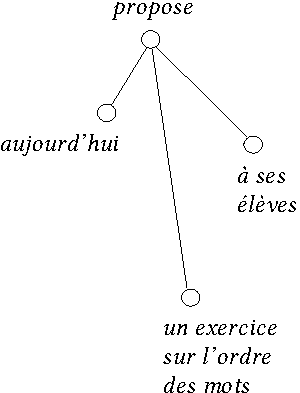
\includegraphics[scale=0.9]{figures/polygraphs/graph-3.5.22.pdf}
\end{figure}

    La position finale d’un dépendant se trouve alors déterminée par la «~longueur~» initiale de la dépendance (déterminée par la fonction et la nature du dépendant comme dans le modèle avec gabarit), l’\hi{élasticité} de cette dépendance et différents paramètres comme le poids ou la saillance.
}
\globe[sec:3.5.23]{Les langues dites à ordre libre}{%
    Une langue est dite \textstyleTermesapprof{à ordre libre} quand une tête et ses dépendants (et notamment le verbe, son sujet et son objet) peuvent être dans n’importe quel ordre. Lorsque, au contraire, un seul ordre est possible, on dit que la langue est \textstyleTermesapprof{à ordre rigide}. Il existe entre les deux toute une gamme de langues à ordre plus ou moins libre ou plus ou moins rigide.

    L’ordre des mots en français est particulièrement rigide, même s’il l’est un peu moins qu’en anglais. L’allemand a un ordre plus libre que le français. Par exemple, on peut traduire \textit{Marie poursuit Pierre} par \textit{die Marie verfolgt den Pierre} ou bien par \textit{den Pierre verfolgt die Marie.} Les deux phrases ont le même \hi{contenu informationnel} (voir chapitre~\ref{sec:1.2}), c’est-à-dire qu’elles décrivent le même état du monde : chaque fois c’est Marie qui poursuit Pierre et pas l’inverse. Le repérage des dépendants du verbe est effectué en allemand grâce à un \textstyleTermesapprof{système casuel}, c’est-à-dire des marques sur certains mots du syntagme substantival qui n’ont pas d’autre rôle que justement d’indiquer la relation qu’entretient le syntagme avec le verbe. Ce sont avant tout les déterminants qui portent l’information casuelle en allemand (voir la \sectref{sec:3.3.26} sur le «~\textit{Déterminant comme tête} ?~»). Dans notre exemple, le fait que \textit{den Pierre} soit l’objet est marqué par le cas accusatif du déterminant masculin singulier \textit{den} (qui s’oppose à la forme nominative \textit{der} de l'article défini).

    L’ordre des mots en allemand n’est cependant pas totalement libre, au sens où seuls deux des six ordres possibles entre les trois mots correspondant à \textit{Marie}, \textit{Pierre} et \textit{poursuit} sont possibles pour une phrase déclarative. Il existe d’autres langues, comme les langues slaves ou le grec moderne, où les six ordres des trois mots sont acceptables et désignent le même état du monde. Voici un exemple du russe :
    
\ea\label{ex:malinu}
    \ea\itshape    Vanya prigotovil malinu\\
    \glt  ‘Vanya a préparé les framboises’ \\
    \glt  ‘Ce que Vanya a préparé, c’est les framboises’

    \ex\itshape Prigotovil Vanya malinu
    \glt ‘Ce qu’a préparé Vanya, c’est les framboises’

    \ex\itshape Malinu prigotovil Vanya
    \glt  ‘C’est les framboises qu’a préparé Vanya’

    \ex\itshape Malinu Vanya prigotovil
    \glt   ‘C’est les framboises que Vanya a préparé’

    \ex\itshape Prigotovil malinu Vanya
    \glt ‘Ce qu’il a préparé, c’est les framboises, Vanya’

    \ex\itshape Vanya malinu prigotovil
    \glt  ‘Vanya, c’est les framboises qu’il a préparé’
\z
\z
    Nous avons donné ici les traductions en français lorsque ces phrases répondent à une question sous-jacente telle \textit{Qu’a préparé Vanya} ?, c’est-à-dire que \textit{malinu} ‘les framboises’ est le \textstyleTermesapprof{rhème} (ce qu’on dit), tandis que \textit{Vanya prigotovil} ‘Vanya a préparé’ est le \textstyleTermesapprof{thème} (ce dont on parle). Les six ordres en russe s’accompagnent évidemment de légères différences de sens, relevant de la structure communicative (voir l’encadré suivant), similaires à celles que montrent leurs traductions en français. Il n’en reste pas moins que les six ordres sont possibles.

    Si on regarde les traductions françaises, on remarque que les variations entre ces phrases sont constituées de constructions qui servent à mettre en avant un élément de la phrase. La construction clivée en «~\textit{C’est … que}~», appelée \textstyleTermesapprof{clivée} (voir le Test de clivage dans la \sectref{sec:3.4.9}) est utilisée dans les traductions des phrases (\ref{ex:malinu}c, d et f) pour mettre en valeur un élément rhématique non verbal~(ici \textit{les framboises}). À cette construction s’oppose la \textstyleTermesapprof{dislocation gauche}, qui sert à distinguer un élément thématique, comme \textit{Vanya} dans la traduction de la phrase (\ref{ex:malinu}f). Similairement, on peut aussi disloquer un élément thématique à droite, comme \textit{Vanya} dans la traduction de phrase (\ref{ex:malinu}e). Enfin, la construction \terme{pseudo-clivée} en «~Ce que …, c’est … » utilisée pour les traductions des phrases (\ref{ex:malinu}a, b et e), combine un clivage avec une dislocation gauche.  
    
    
    Notez ensuite que, abstraction faite des mots fonctionnels des différentes constructions, dans les deux langues considérées, le russe et le français, les trois mots lexicaux se trouvent toujours dans le même ordre. À cela s’ajoute que les principaux prosodèmes, qui constituent l’intonation de la phrase se ressemblent pour chacun des ordres possibles. La phrase (\ref{ex:malinu}b) par exemple, a une courbe intonative que l’on peut schématiser comme suit, avec une intonation montante sur le thème (\textit{prigotovil Vanya}) et une intonation descendante sur le rhème (\textit{malinu}).

    \ea
    \attop{%
    \begin{tikzpicture}
    \matrix (matrix) [matrix of nodes, nodes in empty cells, column sep=3mm, row sep=-8pt,
                      ampersand replacement=\&,every node/.style={font=\strut,anchor=base west}]
      {
        \phantom{Vrigotovil} \& \phantom{Vanya}\&  \vphantom{V}\hphantom{alinu}\\
        \textit{Prigotovil}  \& \textit{Vanya} \&  \textit{malinu}\\
        ‘Ce que prépare      \&   Vanya,       \& c’est les framboises’\\
      }; 
      \draw (matrix-1-1.west) -- (matrix-1-2.center) -- (matrix-1-2.north east);
      \draw (matrix-1-3.north west) -- (matrix-1-3.north) -- (matrix-1-3.east);
    \end{tikzpicture}}
    \z

    Il paraît évident qu’il existe, dans les langues naturelles, une relation entre l’existence d’un système casuel et la liberté dans le placement des arguments verbaux : il serait en effet redondant d’obliger un objet à la fois à porter un marqueur casuel d’accusatif \textit{et} à occuper une place fixe. L’inverse, par contre, n’est pas tout à fait vrai. Une langue sans système casuel n’est pas forcément très restrictive quant à l’ordre des arguments verbaux. Un bel exemple est l'indonésien (et sa variante dialectale, le malais), qui ne connaît pas de flexion casuelle et permet pourtant une plus grande liberté de mots que d’autres langues sans flexion. Si l’ordre dominant est l’ordre SVO comme dans la phrase (\ref{ex:bahasa}a), il est possible de postposer le sujet comme en b et d’antéposer l’objet comme en c.
    
    \ea\label{ex:bahasa}
    \ea
    \gll Ali baca buku itu.\\
    Ali lire    livre  ce\\
    \glt  ‘Ali lit ce livre’
    \ex
    \gll baca buku itu Ali.\\
    lire    livre  ce Ali\\
    \glt  ‘Il lit ce livre, Ali’
    \ex
    \gll buku itu Ali baca.\\
        livre ce Ali lire    \\
    \glt  ‘Ce livre, Ali le lit’
    \z
    \z

    On peut comparer cette situation avec celle que propose le français à l’oral, où, avec les dislocations gauches et droites, les six ordres sont possibles sans qu’il n’y ait aucune marque casuelle indiquant les rôles syntaxiques de \textit{Ali} et \textit{ce livre} :

    \ea
    \ea\itshape {Ali, ce livre, il le lit.}
    \ex\itshape {Ali, il le lit, ce livre.}
    \ex\itshape {Il le lit, Ali, ce livre.}
    \ex\itshape {Ce livre, Ali, il le lit.}
    \ex\itshape {Ce livre, il le lit, Ali.}
    \ex\itshape {Il le lit, ce livre, Ali.}
    \z
    \z
C'est la sémantique de \textsc{lire} et le caractère animé de \textit{Ali} et non animé de \textit{ce livre} qui permet de savoir qui est sujet ou objet du verbe.
}
\globe[sec:3.5.24]{Ordre communicativement dirigé}{%
    Les \hi{langues à ordre rigide} (voir l’encadré qui précède) sont généralement des langues où la position topologique est fortement déterminée par la fonction syntaxique et la catégorie syntaxique. Ainsi, en français, un objet direct doit nécessairement être après le verbe, à moins que ce soit un clitique, un pronom relatif ou un pronom interrogatif. Autrement dit, en français, l’ordre linéaire est utilisé pour marquer la fonction syntaxique et permettre le repérage de l’objet par rapport au sujet. Nous dirons que de telles langues ont un \textstyleTermesapprof{ordre syntaxiquement dirigé}.

    A l’inverse dans \hi{les langues à ordre libre}, la fonction syntaxique joue peu de rôle, puisque, quelle que soit la fonction syntaxique, tous les ordres sont possibles. Il ne faut pas croire pour autant que l’ordre dans ces langues soit non motivé et que tous les ordres se valent. Il existe un \hi{principe d’économie} qui veut que les langues cherchent à en dire le maximum avec le minimum de moyens : il n’est donc même pas imaginable qu’un moyen aussi disponible que l’ordre linéaire ne soit pas exploitée par la grammaire. À quelle fin est alors utilisé l’ordre linéaire quand il ne sert pas à exprimer la fonction syntaxique ?

    Il semble que, dès que l’ordre n’est pas syntaxiquement dirigé, il serve principalement à exprimer la \textstyleTermesapprof{structure communicative} (voir l’\encadref{sec:1.2.4} sur \textit{Les composantes du sens}) et en particulier à indiquer de quoi on parle et ce qu’on en dit (l’\textstyleTermesapprof{opposition thème/rhème}) et ce que l’on souhaite contraster (la \textstyleTermesapprof{focalisation}). Les langues à ordre libre sont donc généralement des langues à \textstyleTermesapprof{ordre communicativement dirigé}.

    Nous avons vu, dans l’encadré qui précède, que le russe permettait tous les ordres possibles du verbe avec son sujet et son objet. Les traductions que nous avons proposées montrent que ces variations d’ordres correspondent en français à des constructions telles que le clivage ou la dislocation. En français, le clivage sert à marquer un \hi{rhème focalisé~}: autrement dit, dans la phrase \textbf{\textit{C’est}} \textit{les framboises} \textbf{\textit{que}} \textit{Vanya préfère}, non seulement \textit{les framboises} est rhématique (ce qu’on dit, l’information qui est communiquée, c’est \textit{les framboises}), mais en plus cette information est \textstyleTermesapprof{focalisée}, c’est-à-dire qu’elle est contrastée avec tous les autres éléments qui pourraient occuper cette position : c’est les framboises que Vanya préfère, à l’exclusion de toutes les autres choses pertinentes dans le contexte d’énonciation. La dislocation gauche quant à elle sert à marquer un \hi{thème focalisé~}: autrement dit, dans la phrase \textit{Les framboises, Vanya aime ça}, non seulement \textit{les framboises} est thématique (ce dont on parle, ce qui est le thème de l’information que je vais communiquer, c’est \textit{les framboises}), mais en plus cette information est focalisée, c’est-à-dire qu’elle est contrastée avec tous les autres éléments qui pourraient occuper cette position dans le contexte d’énonciation : les framboises, il aime ça, les autres fruits rouges, c’est moins sûr.

    
    \begin{figure}[H]
    \caption{Gabarit topologique de la phrase en russe\label{fig:topo-russe}}
    \begin{tabular}{|c|c|c|}
     \hline
    \multicolumn{3}{|c|}{\cellcolor{lsDOIGray}Domaine principal}\\
    \hhline{---}
    thème-foc & rhème & thème\\
    \hhline{---}
    \end{tabular}
    \end{figure}

    On peut postuler qu’en russe, l’ordre linéaire de la phrase obéit au gabarit de la figure~\ref{fig:topo-russe}.
    Le verbe en fonction de sa valeur communicative va venir dans un des trois champs. Les dépendants qui on la même valeur communicative que lui se placeront dans le même champ, tandis que ceux qui ont d’autres valeurs iront dans d’autres champs. La prosodie viendra souligner cette répartition avec une intonation montante sur le thème focalisé, descendante sur le rhème et généralement plate sur le thème.

    C’est à Henri Weil, dans sa thèse publiée en \citeyear{weil1844de} (déjà mentionnée dans l’\encadref{sec:3.5.12} sur les \textit{Langues à têtes finales et langues à têtes initiales} et dans l’\encadref{sec:3.5.21} sur les \textit{Préférences dans l’ordre : rejet des constituants lourds}), que l’on doit d’avoir introduit les notions de thème et rhème et d’avoir noté que trois facteurs pouvaient influencer l’ordre des mots : la structure de dépendance, la structure communicative et la prosodie. En comparant le français, l’anglais, l’allemand, le turc, le chinois, le latin et le grec ancien, il remarque que certaines langues ont un ordre davantage contrôlé par la syntaxe (les langues dites à ordre rigide) et d’autres davantage contrôlé par la structure communicative (les langues dites à ordre libre).
}
\largerpage[2]
\loupe[sec:3.5.25]{Les autres usages de l’ordre linéaire}{%
    Nous venons de voir, dans les deux encadrés qui précèdent, les deux principaux usages de l’ordre linéaire : le marquage de la fonction syntaxique et le marquage de la structure communicative. Il existe trois autres usages de l’ordre linéaire.

    Premièrement, certains syntaxèmes peuvent avoir des contraintes de placement très particulières. En arabe, par exemple, le déterminant défini se place devant le nom (\textit{\textbf{al}-}ʔ\textit{awlaad-u}, \textsc{def}-enfant-\textsc{nom.pl} ‘les enfants’), alors que l’indéfini se place après (\textit{ʔawlaad-u-\textbf{n}}, enfant-\textsc{nom.pl-indef} ‘des enfants’). En français, certains adjectifs tendent à se placer devant le verbe (\textit{un} \textbf{\textit{petit}} \textit{ballon}), certains se placent obligatoirement après (\textit{un ballon} \textbf{\textit{rouge}}), tandis que, pour d’autres encore, l’ordre est relativement libre (\textit{un} \textbf{\textit{superbe}} \textit{ballon~}; \textit{un ballon} \textbf{\textit{superbe}}). Certains adjectifs peuvent avoir selon leur acception des placements différents : \textit{un homme grand} (un homme grand parmi les hommes) vs \textit{un grand homme} (un homme grand dans l’humanité), \textit{un marié jeune} (une personne jeune parmi les mariés) vs \textit{un jeune marié} (une personne jeune dans son mariage).

    Deuxièmement, les mêmes éléments lexicaux peuvent selon l’ordre déclencher des constructions différentes. Tel est le cas en russe : le numéral se place normalement devant le nom, comme dans \textit{sto metrov} ‘cent mètres’, mais on peut aussi placer le numéral après le nom. Néanmoins, il s’agit d’une autre construction, car le sens change : \textit{metrov sto} ‘approximativement cent mètres’.

    Troisièmement, les différences d'ordre des mots entraînent des différences de portée et donc de sens : \textit{Le lundi, Pierre travaille à Paris} (chaque lundi Pierre est à Paris) vs À \textit{Paris, Pierre travaille le lundi} (quand Pierre n’est pas à Paris on ne sait pas ce qu’il fait le lundi). On peut imputer la différence de sens des deux phrases à une différence de structure communicative : dans la première \textit{lundi} est un thème focalisé, alors que c’est \textit{à Paris} dans la deuxième. Néanmoins, la différence de portée entraîne aussi une différence de sens informationnel, puisque les deux phrases peuvent correspondre à des situations du monde différentes.
}
\section{Modèle topologique}\label{sec:3.5.26}

Nous avons défini le modèle topologique comme le module grammaticale assurant la linéarisation (voir la \sectref{sec:3.5.6} sur la \textit{Linéarisation}). Mais quand on nomme ce module le modèle topologique, on fait généralement référence à une modélisation basée sur les gabarits et induisant une structure topologique. Nous allons présenter ce modèle plus en détail.

Nous avons donné le gabarit topologique du verbe à l’indicatif en français dans la figure~\ref{fig:domaine-verbal}. Nous donnons le gabarit topologique du nom en français dans la figure~\ref{fig:domaine-nominal}.
Le nom possède un champ final à sa droite où les compléments peuvent se placer assez librement (avec des préférences en fonction de leur poids et de leur saillance), tandis que l’ordre à gauche du nom est assez rigide : ainsi, un syntagme comme \textit{les deux seules autres petites tables} n’accepte pas d’autre ordre que celui qu’il a. Voir l’\encadref{sec:3.5.27} sur la \textit{Topologie du groupe substantival en français}.

\begin{figure}\small
\caption{Gabarit topologique du domaine nominal\label{fig:domaine-nominal}}
\begin{tabular}{|c|c|c|c|c|c|c|c|c|}
\hline
\multicolumn{9}{|c|}{\cellcolor{lsDOIGray}Domaine nominal}\\
\hline
\rotatebox{90}{ch-tout} &  \rotatebox{90}{ch-article~} &  \rotatebox{90}{ch-num} &  \rotatebox{90}{ch-seul} &  \rotatebox{90}{ch-autre} &  \rotatebox{90}{ch-adj} &  \cellcolor{lsDOIGray}\rotatebox{90}{ch-nom} &  \rotatebox{90}{ch-deN} &  \rotatebox{90}{ch-final}\\
\hline
\end{tabular}
\end{figure}

Voyons maintenant comment linéariser un arbre de dépendance. Nous redonnons dans la figure~\ref{fig:ballon-dep2} l'arbre de dépendance discuté dans la \sectref{sec:3.5.19} sur \textit{La linéarisation des codépendants}.

\begin{figure}
\begin{tikzpicture}
    \begin{scope}[every node/.style={CircleNode},level distance=2\baselineskip,
                  level 1/.style={sibling distance=20mm},
                  level 2/.style={sibling distance=15mm},
                  level 3/.style={sibling distance=10mm}
                  ]
      \node (root) {} child { node{} child { node{} } child { node{} } edge from parent node [reset shape,midway,above] {sujet} }
                      child { node{} }
                      child { node [xshift=-7mm] {} }
                      child { node [xshift=-7mm] {} }
                      child { node [xshift=-7mm] {} child { node [xshift=5mm] {} } child { node [xshift=5mm] {} } child { node [xshift=5mm] {} } edge from parent node [reset shape,midway,above] {objet} };
    \end{scope}
    \begin{scope}[every node/.style={font=\itshape\strut}]
    \node [above=1pt of root] {prêtera};
    \node [left=1pt of root-1] {garçon};
    \node [below=1pt of root-1-1] {le};
    \node [below=1pt of root-1-2] {petit};
    \node [below=1pt of root-2] {lui};
    \node [below=1pt of root-3] {ne};
    \node [below=1pt of root-4] {pas};
    \node [right=1pt of root-5] {ballon};
    \node [below=1pt of root-5-1] {son};
    \node [below=1pt of root-5-2] {gros};
    \node [below=1pt of root-5-3] {autre};
    \end{scope}
\end{tikzpicture}
\caption{\label{fig:ballon-dep2}Arbre de dépendance de \REF{ex:ballon}}
\end{figure}

Nous procédons en parcourant l’arbre de dépendance à partir de la racine. On commence donc par considérer le verbe \textit{prêtera} qui va ouvrir un domaine verbal. Les règles d’ordre indiquent pour chaque dépendant dans quel champ il peut aller en fonction de sa nature et de sa fonction : un sujet peut aller dans le champ ch-initial, un clitique dans un champ ch-cl-X, etc. On obtient au final la configuration suivante (où les champs non remplis ne sont pas représentés) :

\ea\hfill \begin{tabular}{|c|c|c|c|c|c|}
\hline
garçon & ne & lui & \cellcolor{lsDOIGray}prêtera & pas & ballon\\
\hline
\end{tabular}
\hfill\hbox{}\z

Chaque mot va ensuite ouvrir dans la position qu’il occupe un constituant topologique qui accueillera ses dépendants. Le gabarit du constituant dépendra de la nature de l’élément qui l’ouvre et du champ qu’il occupe (pour le rôle joué par le champ dans le choix du gabarit, voir le cas des adjectifs du français dans l’\encadref{sec:3.5.27} qui suit, et celui des verbes en allemand dans l’\encadref{sec:3.5.36} sur \textit{La structure topologique de l’allemand}). Ainsi les noms \textit{garçon} et \textit{ballon} vont-ils ouvrir des domaines nominaux, pour accueillir leurs dépendants, et donner l’ordre final suivant :

\ea\label{ex:topo-ballon}%
\resizebox{.995\linewidth}{!}{\def\arraystretch{1.5}\begin{tabular}{|l|l|l|l|l|l|}
\hline
& & &\cellcolor{lsDOIGray} & & \\[-18pt]
  {\def\arraystretch{1}
  \begin{tabular}{@{}|l|l|l|@{}}
  \hline
    \rotatebox{0}{le} & \rotatebox{0}{petit} & \cellcolor{lsDOIGray} \rotatebox{0}{garçon}\\
  \hline
  \end{tabular}}
  & \rotatebox{0}{ne} & \rotatebox{0}{lui} & \cellcolor{lsDOIGray} \rotatebox{0}{prêtera} & \rotatebox{0}{pas} &
  {\def\arraystretch{1}
  \begin{tabular}{@{}|l|l|l|l|@{}}
    \hline
    \rotatebox{0}{son} & \rotatebox{0}{autre} & \rotatebox{0}{gros} & \cellcolor{lsDOIGray} \rotatebox{0}{ballon}\\
    \hline
  \end{tabular}}\\[-15pt]
   & & &\cellcolor{lsDOIGray} \raisebox{5.5pt}{prêtera} & & \\
\hline
\end{tabular}}\z

On notera qu’en plus de l’ordre linéaire, nous avons obtenu une structure avec des constituants emboîtés.\largerpage

\Definition{\textstyleTermes{structure topologique}}{La structure d'\hi{emboîtement} que forme les \hi{constituants topologiques} est appelée la \textstyleTermes{structure topologique}. Dans une structure topologique, chaque constituant occupe un \hi{champ topologique}.}

La structure topologique est un \textstyleTermes{arbre de constituants ordonné}, c’est-à-dire un arbre de constituants  avec un ordre linéaire sur les fils de chaque nœud (voir l’\encadref{sec:3.5.28} sur l'\textit{Arbre de constituants ordonné}). Dans le cas de la structure topologique, l’ordre linéaire sur les fils d’un nœud est donné par le gabarit du constituant, qui est une liste linéairement ordonnée de champs. Les structures topologiques se distinguent notamment des arbres de constituants syntaxiques par le fait que chaque constituant est associé à un champ topologique.

La structure topologique de l'exemple \REF{ex:ballon} est donnée sous la forme d'un emboîtement de constituants en \REF{ex:topo-ballon} et sous forme d'arbre dans la figure~\ref{fig:topo-ballon}. La deuxième représentation comporte en plus des étiquettes catégorielles sur les constituants topologiques. Il est encore possible d'enrichir la représentation en ajoutant  le nom du champ occupé par chaque constituant sur la relation partie-tout avec le constituant père.

\begin{figure}
\resizebox{\textwidth}{!}{\begin{tikzpicture}
    \begin{scope}[every node/.style={CircleNode},level distance=2\baselineskip,
                  level 1/.style={sibling distance=18mm},
                  level 2/.style={sibling distance=9mm},
                  ]
      \node (root) {} child { node{} child { node{} } child { node{} } child { node{} } } 
                      child { node [xshift = 3mm] {} }
                      child { node [xshift = 1mm] {} }
                      child { node [xshift = -1mm] {} }
                      child { node [xshift = -3mm] {} }
                      child { node{} child { node{} } child { node{} } child { node{} } child { node{} } }; 
    \end{scope}
    \node [above=1pt of root] {domaine verbal};
    \node [above left=1pt of root-1,align=center] {\strut domaine\\nominal};
    \node [above right=1pt of root-6,align=center] {\strut domaine\\nominal};
    \begin{scope}[every node/.style={font=\itshape\strut}]
    \node [below=1pt of root-1-1] {le};
    \node [below=1pt of root-1-2] {petit};
    \node [below=1pt of root-1-3] {garçon};
    \node [below=1pt of root-2] {ne};
    \node [below=1pt of root-3] {lui};
    \node [below=1pt of root-4] {prêtera};
    \node [below=1pt of root-5] {pas};
    \node [below=1pt of root-6-1] {son};
    \node [below=1pt of root-6-2] {autre};
    \node [below=1pt of root-6-3] {gros};
    \node [below=1pt of root-6-4] {ballon};
    \end{scope}
\end{tikzpicture}}
\caption{\label{fig:topo-ballon}Arbre topologique}
\end{figure}

\largerpage
\eiffel[sec:3.5.27]{Topologie du groupe substantival en français}{%
    Dans le gabarit pour le nom de la figure~\ref{fig:domaine-nominal} figure un champ ch-deN, juste après le champ qu’occupe le nom. Il existe en effet une contrainte d’ordre qui concerne les compléments en \textit{de} N (préposition \textsc{de} suivi d’un \hi{nom nu}, c’est-à-dire sans déterminant). Prenons l’exemple des dépendants possibles du syntagme \textit{une chemise}. Nous pouvons modifier \textit{une chemise} par \textit{pour homme}, \textit{en coton} ou \textit{pour le sport}. Chacun de ces trois compléments peut aussi être réalisé par un complément en \textit{de} N : \textit{d’homme}, \textit{de coton}, \textit{de sport}. 
    Contrairement à leurs équivalents, les compléments en \textit{de} N supportent très mal d’être séparé du nom : alors qu’on dira
    (\ref{ex:coton}a), on dira difficilement (\ref{ex:coton}b) et on préférera (\ref{ex:coton}c).
     
    \ea\label{ex:coton}\judgewidth{\textsuperscript{??}}
    \ea[]{\textit{une chemise orange en coton}}
    \ex[\textsuperscript{??}]{\textit{une chemise orange de coton}}
   \ex[]{\textit{une chemise de coton orange}}
   \z\z
   
   Il semble également difficile de réaliser deux compléments en \textit{de} N, comme en (\ref{ex:coton2}a). Quand on réalise un complément en \textit{de} N avec un autre complément prépositionnel, le complément en \textit{de} N doit précéder l’autre : (\ref{ex:coton2}b) est préférable à (\ref{ex:coton2}c) et (\ref{ex:coton2}d) à (\ref{ex:coton2}e).
  
  \ea\label{ex:coton2}\judgewidth{\textsuperscript{??}}
   \ea[\textsuperscript{??}]{\textit{une chemise de coton de sport}}
   \ex[]{\textit{une chemise de coton pour le sport}}
   \ex[\textsuperscript{??}]{\textit{une chemise pour le sport de coton}}
   \ex[]{\textit{une chemise de sport en coton}}
   \ex[\textsuperscript{??}]{\textit{une chemise en coton de sport}}
   \z
  \z

    Pour les autres dépendants postposés au nom (adjectifs, compléments prépositionnels, participiales, relatives), nous considérons qu’ils vont tous dans un même champ, car leur ordre est relativement libre et semble suivre avant tout des contraintes de poids. Ainsi un adjectif se placera plutôt avant un complément prépositionnel (\textit{un mur ancien en pierre}), mais pour peu que cet adjectif soit un peu plus lourd, il se place sans difficulté après le complément prépositionnel (\textit{un mur en pierre très ancien}).

    L’ordre des éléments antéposés au nom est lui très contraint. De plus, seul des groupes adjectivaux légers peuvent être antéposés :
    on a (\ref{ex:mur}a et b), mais pas (\ref{ex:mur}c), où \textit{haut de trois mètres} doit obligatoirement être postposé au nom comme en (\ref{ex:mur}d)
    (voir aussi l’\encadref{sec:3.5.22} sur \textit{Une modélisation des contraintes de poids}). 
    
    \ea\label{ex:mur}
    \ea[]{\textit{un} \textbf{\textit{haut}} \textit{mur}}
    \ex[]{\textit{un} \textbf{\textit{très haut}} \textit{mur}}
    \ex[*]{\textit{un} \textbf{\textit{haut de trois mètres}} \textit{mur}}
   \ex[]{\textit{un mur} \textbf{\textit{haut de trois mètres}}}
    \z
    \z
    Du point de vue du modèle topologique, cela signifie que l’adjectif \textit{haut} n’ouvre pas un domaine adjectival complet lorsqu’il est antéposé, mais un \textstyleTermes{domaine réduit} où ne figure pas le champ final qui accueille normalement les compléments de l’adjectif. Voir la figure~\ref{fig:domaine-adj} : le domaine adjectival complet est utilisé à droite du verbe comme en (\ref{ex:mur}d), tandis que le domaine réduit est utilisé à gauche du verbe comme en (\ref{ex:mur}a et b), ce qui bloque (\ref{ex:mur}c), puisqu'il n'y a pas de place pour le complément prépositionnel de l'adjectif.
    
\begin{figure}[H]
    \caption{Gabarits pour les domaines adjectivaux}
    \label{fig:domaine-adj}
        \begin{center}
    \def\arraystretch{1.5}
    \setlength{\tabcolsep}{4ex}
    \begin{tabular}{|c|c|c|}
    \hline
    \multicolumn{3}{|c|}{\cellcolor{lsDOIGray}Domaine adjectival}\\\hline
    ch-adv & \cellcolor{lsDOIGray} ch-adjectif & ch-final\\
    \hline
    \end{tabular}
    \end{center}
   \begin{center}
    \def\arraystretch{1.5}
    \setlength{\tabcolsep}{4ex}
    \begin{tabular}{|c|c|}
    \hline
    \multicolumn{2}{|c|}{\cellcolor{lsDOIGray}Domaine adjectival réduit}\\\hline
    ch-adv & \cellcolor{lsDOIGray}ch-adjectif\\
    \hline
    \end{tabular}
    \end{center}
\end{figure}

Quant à l’ordre relatif des adjectifs antéposés, évoqué à la \sectref{sec:3.5.26}, il semble aller des \hi{éléments à valeur référentielle} à des \hi{adjectifs qualificatifs}. Ces derniers qualifient le référent, en précisent la nature, tandis que les premiers précisent la nature de la référence elle-même : l’article indique si le référent est connu ou pas, le numéral donne le nombre de référents, des adjectifs comme \textit{seul} ou \textit{autre} permettent de positionner le référent dans l’ensemble des référents potentiels.
}
\largerpage
\maths[sec:3.5.28]{Arbre de constituants ordonné}{%
En définissant la structure topologique dans la \sectref{sec:3.5.26} sur le {\textit{Modèle topologique}}, nous avons introduit rapidement la notion d'\terme{arbre de constituants ordonné}. Nous allons préciser la nature de cette structure et les modes de représentation associés.

    
L’\hi{ordre linéaire sur les fils de chaque nœud} \hi{interne} de l’arbre induit un unique \hi{ordre linéaire sur les feuilles} de l’arbre. Et réciproquement, l’ordre linéaire sur les feuilles suffit à récupérer l’ordre linéaire sur les fils de chaque nœud interne. La preuve est relativement simple : pour ordonner deux feuilles, il faut rechercher leur premier ancêtre commun, lequel est unique. L’ordre sur les deux feuilles considérées est le même que celui des deux fils de leur ancêtre commun qui se trouvent sur les deux branches qui mènent à elles. Par exemple, pour ordonner \textit{garçon} et \textit{ne} dans l’exemple \REF{ex:ballon}, il faut remonter à leur ancêtre commun qui est le nœud du domaine verbal. On en déduit que \textit{garçon} est avant \textit{ne}, car le domaine nominal est avant \textit{ne}.

La preuve que nous venons de faire n'est valable que parce que nous ne considérons que des constituants \textit{continus}. Les constituants topologiques sont continus par définition. Les constituants syntaxiques peuvent être discontinus, mais ils ne pourront pas alors être représentés par des structures de constituants ordonnés (voir l'\encadref{sec:3.2.7}  \textit{De la non-séparation des ordres au mouvement}).

Contrairement au cas des arbres de dépendance ordonnés dont les nœuds sont totalement ordonnés, l’\hi{ordre} sur les nœuds d’un arbre de constituants est \hi{partiel}, puisque deux constituants qui sont dans une relation de partie-tout ne peuvent être dans une relation de précédence l’un par rapport à l’autre et que donc une telle spécification d’ordre ne serait pas pertinente.


Nous allons maintenant discuter un point important concernant la représentation des arbres de constituants ordonnés.
On peut voir les «~nœuds~» de l’arbre de constituants ordonné non pas comme de simples nœuds, mais comme des segments ayant un début et une fin. N’oublions pas que les nœuds d’un arbre de constituants sont des constituants d’un énoncé et que les constituants d’un énoncé sont des segments continus de cet énoncé. On peut alors représenter les constituants comme des arcs allant d’un nœud début à un nœud fin.  Lesquels nœuds correspondent en fait aux positions linéaires inter-mot (si les constituants minimaux sont les mots) (voir l'\encadref{sec:3.5.17} sur le \textit{{Flux de dépendances}}, où il a déjà été question des positions inter-mot).
Nous allons expliciter ce point en proposant deux représentation du même arbre de constituants ordonné de la phrase :\smallskip\\
\ea\textit{Le chat poursuit un chien.}\z

La première représentation, donnée dans la figure~\ref{fig:arbre-tradi},
est
la \hi{représentation traditionnelle} d'un arbre de constituants ordonné du type syntaxe X-barre (voir l’\encadref{sec:3.4.19} sur la \textit{Syntaxe X-barre}). Dans cette représentation de l'arbre de constituants ordonné,
la \hi{structure d'arbre} est \hi{explicite} et
l'\hi{ordre} est \hi{implicite}, c’est-à-dire qu’il est représenté par la \hi{position relative des nœuds sur l’axe horizontal}, mais n’est pas explicitement encodé par des relations de précédence entre nœuds.

\begin{figure}[H]
    \caption{Représentation traditionnelle d'un arbre de constituants ordonné (hiérarchie explicite, ordre implicite)\label{fig:arbre-tradi}}
    \begin{forest}
    [\textrm{P}
      [GN [D [\textit{le}]] [N [\textit{chat}]] ]
      [GV [V [\textit{poursuit}]] [GN [D [\textit{un}] ] [N [\textit{chien}] ] ] ]
    ]
    \end{forest}
 \end{figure}

\begin{figure}[H]
    \caption{Représentation en cellules d'un arbre de constituants ordonné (hiérarchie implicite, ordre explicite)\label{fig:arbre-cellule}}
\begin{tikzpicture}
    \begin{scope}[every node/.style={CircleNode},grow=right]
    \node (root) {} child { node {} child { node{} child { node{} child { node{}  
                    child { node{} } } } } }; 
    \end{scope}      
     \path (root)         edge[bend left] node[midway, above] {D} (root-1)
           (root-1)       edge[bend left] node[midway, above] {N} (root-1-1)
           (root-1-1)     edge[bend left] node[midway, above] {V} (root-1-1-1)
           (root-1-1-1)   edge[bend left] node[midway, above] {D} (root-1-1-1-1)
           (root-1-1-1-1) edge[bend left] node[midway, above] {N} (root-1-1-1-1-1)
           (root)         edge[bend left=66] node[midway, above] {GN} (root-1-1)
           (root-1-1-1)   edge[bend left=66] node[midway, above] {GN} (root-1-1-1-1-1)
           (root-1-1)     edge[bend left=90] node[midway, above] {GV} (root-1-1-1-1-1)
           (root)         edge[bend left=90] node[midway, above] {P} (root-1-1-1-1-1);
           
     \coordinate (1) at ($ (root) !.5! (root-1) $);
     \coordinate (2) at ($ (root-1) !.5! (root-1-1) $);
     \coordinate (3) at ($ (root-1-1) !.5! (root-1-1-1) $);
     \coordinate (4) at ($ (root-1-1-1) !.5! (root-1-1-1-1) $);
     \coordinate (5) at ($ (root-1-1-1-1) !.5! (root-1-1-1-1-1) $);
     
    \foreach \pos/\text in {1/le,2/chat,3/poursuit,4/un,5/chien} 
      {\node [font={\itshape\strut}, below=1pt of \pos] {\text};}
\end{tikzpicture}
 \end{figure}
 
\begin{figure}[H]
\caption{Variante simplifiée de la représentation en cellules d'un arbre de constituants ordonné\label{fig:arbre-cel2}}
\begin{tikzpicture}[decoration={brace, 
                                mirror, 
                                raise=-.25\baselineskip}]
    \matrix (matrix) [matrix of nodes,
                      nodes in empty cells, 
                      ampersand replacement=\&, 
                      nodes = {font=\strut},
                      column sep=1em,
                      column 1/.style={nodes={minimum width=1.4em}},
                      column 2/.style={nodes={minimum width=2.5em}},
                      column 3/.style={nodes={minimum width=4.125em}},
                      column 4/.style={nodes={minimum width=1.75em}},
                      column 5/.style={nodes={minimum width=3em}}]
      {
    \textit{le} \& \textit{chat} \& \textit{poursuit} \& \textit{un} \& \textit{chien}\\
        D \& N \& V \& D \& N\\
          \&   \&   \&   \& \\
          \&   \&   \&   \& \\
          \&   \&   \&   \& \\		      		      
      }; 
    
    \draw[decorate] 
      (matrix-2-1.south west) -- (matrix-2-2.south east) 
      node [midway, below] {GN};
    
    \draw[decorate] 
      (matrix-2-4.south west) -- (matrix-2-5.south east)
      node [midway, below] {GN};
      
    \draw[decorate] 
      (matrix-3-3.south west) -- (matrix-3-5.south east)
      node [midway, below] {GV};
      
    \draw[decorate] 
      (matrix-4-1.south west) -- (matrix-4-5.south east)
      node [midway, below] {P};
         
  
    \foreach \i in {1,...,5} 
      {
        \draw (matrix-1-\i.south west) -- (matrix-1-\i.south east);
      }
\end{tikzpicture}
\end{figure}

Dans la deuxième représentation, donnée dans la figure~\ref{fig:arbre-cellule},  l’\hi{ordre} est \hi{explicite} et la \hi{structure d'arbre} est \hi{implicite} et peut se déduire de la \hi{position relative des constituants sur l’axe vertical}. Les nœuds du graphe représentent les \hi{positions inter-mot} et les constituants sont représentés par des arcs qui relient leur début à leur fin.  Bien que cette représentation soit  moins usuelle, elle est tout aussi simple et légitime que la représentation traditionnelle.  Cette représentation, où chaque décomposition d'un constituant (chaque connexion vue du point de vue dépendentiel) forme une «~cellule~», sera nommée la \hi{représentation en cellules} d'un arbre de constituants ordonné ou plus simplement un \textstyleTermes{arbre de constituants en cellules}. On la trouve plus souvent dans une version simplifiée, où les positions inter-mot restent implicites, comme dans la figure~\ref{fig:arbre-cel2}.

Notons qu'il est possible de combiner la représentation traditionnelle avec la représentation en cellules et d'expliciter à la fois la structure hiérarchique d'arbre et l'ordre linéaire dans une même représentation. 
}
\maths[sec:3.5.29]{Grammaires de réécriture}{%
    L’une des premières modélisations mathématiques de la grammaire est la \textstyleTermesapprof{grammaire de réécriture} proposée par Noam \citet{chomsky1957syntactic} (voir l’\encadref{sec:1.3.7} sur \textit{Calcul symbolique et grammaires catégorielles} pour les toutes premières grammaires formelles). Notre modèle topologique, au travers de ses gabarits, prolonge ce formalisme. Nous commençons par présenter ce formalisme avant d'en expliquer les limites et de montrer l'intérêt d'introduire un modèle plus riche comme le modèle topologique.

\tcbsubtitle{Exemple}
    Bien qu’on puisse utiliser les grammaires de réécriture pour définir des grammaires de dépendances, il s’agit au départ d’un formalisme introduit pour écrire des grammaires de constituants. Voici un exemple pour ceux qui ne connaissent pas encore ce formalisme. Les \textstyleTermesapprof{règles} (dites \textstyleTermesapprof{de réécriture}) sont de la forme :

    \ea \label{ex:regles}
    \begin{tabular}[t]{@{}l@{\hspace{4\tabcolsep}}l@{}}
    P → GN GV  &  V → \textit{attrape} {\textbar} \textit{poursuit}\\
    GV → V GN  &  N → \textit{chat} {\textbar} \textit{chien}\\
    GN → D N   & D → \textit{le} {\textbar} \textit{un}\\
    \end{tabular}
    \z

    Avec de telles règles, on peut produire des phrases telles que \textit{le chat poursuit un chien} ou \textit{le chien attrape le chat}. Les règles de droite sont des \textstyleTermesapprof{règles lexicales} (par exemple \textit{attrape} ou \textit{poursuit} sont des constituants de type V). Les règles de gauche sont des \textstyleTermesapprof{règles syntagmatiques} qui disent comment un constituant se décompose. Par exemple, la règle P \textrm{→} GN GV dit qu’une phrase P peut se décomposer en un groupe nominal GN suivi d’un groupe verbal GV. Lue autrement, elle dit comment les constituants se combinent : la combinaison d’un GN suivi d’un GV donne un P. La règle P \textrm{→} GN GV ne dit pas seulement que P se décompose en GN et GV, mais aussi que GN précède GV et que l’extension de P est égale à la somme des extensions de GN et GV.

    On peut réinterpréter les règles syntagmatiques comme des \textstyleTermesapprof{structures élémentaires}, c’est-à-dire des portions de la structure finale, un arbre de constituants ordonné dans notre cas, qui, assemblées, permettent de reconstituer la structure finale. La figure~\ref{fig:PGNGV} donne un exemple pour la règle de réécriture P → GN GV. Nous utilisons les deux modes de représentation d’un arbre de constituants ordonné présentés dans l’encadré précédent.

\begin{figure}[H]
% %     \includegraphics{}
    \caption{La règle de réécriture P → GN GV vue comme une structure élémentaire\label{fig:PGNGV}}
    \label{fig:structureGNGV}
    \begin{subfigure}[c]{.5\linewidth}\centering
        \begin{forest} 
        [P [GN] [GV]]
        \end{forest}
        \caption{Représentation en arbre}
        \end{subfigure}\begin{subfigure}[c]{.5\linewidth}\centering
        \begin{tikzpicture} 
       \node at (0,0) (GN) [CircleNode] {};
       \node at (1,-.75) (empty) [CircleNode] {};
       \node at (2,0) (GV) [CircleNode] {};
%        \node [below=1pt of 1] {P};
%        \node [below left = 2pt of GN] {GN};
%        \node [below right = 2pt of GV] {GV};
       \path (GN) edge [out=270,in=180] node [left,midway] {GN} (empty)
             (empty) edge [out=0,in=270] node [right,midway] {GV} (GV)
             (GN) edge [bend left=66] node [below,midway] {P} (GV);
       \end{tikzpicture}
       \caption{Représentation en cellules}
    \end{subfigure}
 \end{figure}

    Avec les règles proposées en \REF{ex:regles}, et en les considérant comme des structures élémentaires qu'on assemble, on peut générer l’arbre de constituants de la phrase \textit{Le chat poursuit un chien} donné dans l’encadré qui précède. Chaque portion élémentaire de l’arbre, composée d’un nœud et de ses fils, correspond exactement à une règle de réécriture. Ainsi le sommet de l’arbre avec le nœud P et ses deux fils GN et GV est validé par la règle P~\textrm{→} GN GV.

  \tcbsubtitle{Critiques}
    Nous souhaitons faire trois critiques concernant une grammaire de constituants comme celle qui précède (qui sert toujours de base à de nombreux modèles linguistiques).

    Passons rapidement sur la première, puisqu’elle a déjà fait abondamment l’objet de ce livre : nous pensons qu’il est plus judicieux de penser la syntaxe d’une langue en termes de connexions et de dépendances qu’en termes de constituants (voir le \chapref{sec:3.2} sur la connexion où nous discutons les problèmes que cela pose de vouloir privilégier une fragmentation parmi toutes celles possibles), bien que, comme nous l’avons montré (\chapref{sec:3.4}), les deux approches sont en grande partie équivalentes.

    La deuxième critique concerne le fait de vouloir \hi{exprimer simultanément la constituance immédiate} (le fait qu’une phrase P peut être décomposée en un GN et un GV) \hi{et l’ordre linéaire} (le fait que GN < GV). Ceci peut encore se comprendre pour des langues à ordre rigide comme l’anglais, mais est difficilement justifiable pour des langues à ordre libre, où l’ordre linéaire dépend peu des relations syntaxiques (voir l’\encadref{sec:3.5.24} sur \textit{Ordre communicativement dirigé}). Cette critique a été faite dès les années 1970 et les modèles qui ont émergé au début des années 1980, notamment GPSG (\textit{Generalized Phrase Structure Grammar}), la Grammaire syntagmatique généralisée de Gerald Gazdar, bien que toujours basée sur une grammaire de réécriture, séparaient clairement les \textstyleTermesapprof{règles} dites \textstyleTermesapprof{de dominance immédiate} des \textstyleTermesapprof{règles de précédence linéaire} entre constituants.

    La troisième critique permet de saisir une différence essentielle entre les \hi{grammaires} dites \hi{syntagmatiques} (\textit{Phrase Structure Grammars} ou PSG) et les grammaires topologiques. Les règles de précédence linéaire des PSG sont des règles de précédence entre constituants, comme par exemple GN < GV. Or le sujet du verbe n’est pas nécessairement un groupe nominal (\textbf{\textit{Qu’il} \textit{vienne}} \textit{me surprendrait ;} \textbf{\textit{Partir maintenant}} \textit{serait plus judicieux)}. Il faut donc distinguer la catégorie et la fonction syntaxique. On peut remplacer cette règle par Sujet < V. C’est déjà mieux, mais les grammaires topologiques vont encore plus loin. Comme nous l’avons déjà souligné, en français, le sujet n’est pas toujours devant le verbe, mais pour qu’il n’en soit pas ainsi, il faut qu’un autre élément vienne occuper sa place. Il ne faut donc pas seulement \textit{{déconnecter} la catégorie de la fonction syntaxique}, mais aussi \textit{déconnecter la {fonction syntaxique} de la position topologique} (c'est-à-dire du \hi{champ} dans notre modélisation). Une grammaire topologique décompose la règle Sujet < V en deux règles : 1) il existe un champ préverbal qui doit être rempli par un et un seul élément et 2) le sujet peut occuper le champ préverbal. (Le fait que le sujet occupe occupe généralement le champ préverbal n'est pas dit dans la règle : cela découle du fait que les règles qui placent le sujet dans un autre champ sont très contraintes et donc rarement déclenchées.)
}
\section{Projection topologique et émancipation}\label{sec:3.5.30}%\largerpage

Comme nous venons de le voir, le modèle topologique, en plus d’assurer la linéarisation de l’arbre de dépendance, lui associe un arbre de constituants ordonné, la structure topologique. En cas de \hi{linéarisation projective}, cet arbre est en fait l’\hi{arbre de constituants syntaxiques plat} obtenu à partir des projections maximales des nœuds de l’arbre de dépendance (voir la \sectref{sec:3.4.4} sur l'\textit{Arbre de constituants plat}).

Nous allons maintenant nous intéresser à la \hi{linéarisation non projective}. Dans ce cas, certaines projections maximales ne sont pas continues. Nous allons voir comment associer un arbre de constituants ordonné avec des constituants continus à un arbre de dépendance, qu’il soit projectif ou non.

\Definition{\textstyleTermes{projection topologique}}
{Pour chaque nœud \textit{x} d’un arbre de dépendance ordonné, nous définissons la \textstyleTermes{projection topologique} de \textit{x} comme le plus grand \hi{segment continu} contenant \textit{x} qui corresponde à une portion connexe de l’arbre de dépendance ayant \textit{x} pour racine.}

Lorsque l’arbre de dépendance est projectif, la projection maximale de chaque nœud est continu et donc la projection topologique d’un nœud est sa projection maximale. Mais, dès qu’un arbre de dépendance est non projectif, la projection topologique de certains nœuds n’est plus leur projection maximale. Reprenons l’exemple \REF{ex:belle-complet} de la \sectref{sec:3.5.14} :

\ea\label{ex:belle}
    \textit{{Une belle est entrée qui voulait les acheter}.}
\z
La projection topologique de \textit{une belle} est \textit{une belle}, alors que sa projection maximale est \textit{une belle qui voulait les acheter}. Par contre, la projection topologique de \textit{est entrée} est bien la phrase entière et donc la projection maximale de \textit{est entrée}.

Les projections topologiques associées à un arbre de dépendance ordonné don\-né forment un arbre de constituants ordonné. Nous appelons cet arbre l’\textstyleTermes{arbre topologique} induit par l’arbre de dépendance ordonné. Il s'agit en général de l'arbre sous-jacent à la structure topologique (qui contient en plus des étiquettes sur la nature des constituants et les champs qu'ils occupent, voir la \sectref{sec:3.5.26} sur le {\textit{Modèle topologique}}). Nous verrons dans l'\encadref{sec:3.5.A} un cas d'\textit{Émanci\-pa\-tion projective}, où l'arbre topologique ne correspond pas à la structure topologique. Par ailleurs, la structure topologique peut être plus riche que l'arbre topologique induit dès que l'on considère des constituants topologiques intermédiaires (voir la \sectref{sec:3.5.34} éponyme).

Nous donnons, dans la figure~\ref{fig:induit-topo}, l'arbre topologique à partir d'un arbre de dépendance à gros grains de l'exemple \REF{ex:belle}. Notons qu'il s'agit d'un arbre de constituants avec tête, puisque chaque constituant topologique est la projection d'une tête. Nous explicitons dans la représentation de cet arbre l'ordre linéaire entre les feuilles afin de bien spécifier qu'il s'agit d'un arbre de constituants ordonné, à ne pas confondre avec un arbre de constituants syntaxiques, comme introduit au \chapref{sec:3.4} et qui n'est pas ordonné.

\begin{figure}
\begin{minipage}[c]{.45\linewidth}\centering
\begin{tikzpicture}[>={Triangle[]}]
  \begin{scope}[every node/.style={CircleNode},grow=right,level distance=2cm]
  \node at (0,0) (root) {} child { node {} child { node{} } };
  \path (root) edge [bend left=45,->] (root-1-1)
        (root-1) edge [bend right,->] (root);
  \end{scope}
  \draw [<-] (root-1) -- ++(0,1.5cm);
  \node [below=1pt of root, font=\itshape\strut] {une belle};
  \node [below=1pt of root-1, font=\itshape\strut] {est entrée};
  \node [below=1pt of root-1-1, font=\itshape,align=center] {\strut qui voulait\\les acheter};
\end{tikzpicture}
\end{minipage}\begin{minipage}[c]{.1\linewidth}\centering
\huge$\Rightarrow$
\end{minipage}\begin{minipage}[c]{.45\linewidth}\centering
\begin{tikzpicture}
  \begin{scope}[every node/.style={CircleNode},sibling distance=20mm]
  \node (root) {} 
    child { node{} } 
    child { node{} edge from parent node [reset shape, midway, right] {T} } 
    child { node{} };
  \draw (root-1) -- (root-2) -- (root-3);
  \end{scope}
  \node [below=1pt of root-1, font=\itshape\strut] {une belle};
  \node [below=1pt of root-2, font=\itshape\strut] {est entrée};
  \node [below=1pt of root-3, font=\itshape,align=center] {\strut qui voulait\\les acheter};
\end{tikzpicture}
\end{minipage}
\caption{\label{fig:induit-topo}Arbre de dépendance ordonné et arbre de constituants topologiques induit}
\end{figure}

Un arbre de dépendance ordonné induit donc deux arbres de constituants avec têtes : un arbre de constituants syntaxiques et un arbre de constituants topologiques. Nous donnons, dans la figure~\ref{fig:induit-synt}, l'arbre de constituants syntaxiques de notre exemple.%\largerpage


\begin{figure}
\begin{minipage}[c]{.45\linewidth}\centering
\begin{tikzpicture}[every node/.style={font=\strut\itshape}]
\begin{scope}[
    every node/.style={CircleNode}
    ]
\node (root) {}
    child { node { } 
          child { node { } }
           };
\end{scope}
\node[left=1pt of root] {est entrée};
\node[left=1pt of root-1] {une belle};
\node[left=1pt of root-1-1, align=center] {qui voulait\\les acheter};
\end{tikzpicture}\end{minipage}\begin{minipage}[c]{.1\linewidth} \huge$\Rightarrow$ \end{minipage}%
\begin{minipage}[c]{.45\linewidth}\centering
\begin{tikzpicture}[every node/.style={font=\strut}]
    \begin{scope}[
    every node/.style={CircleNode},
    sibling distance=20mm,
    level distance=3\baselineskip
    ]
        \node (root) {}
            child { node { } child { node { } edge from parent node [reset shape, midway, anchor=base east] {T} } 
                            child { node { } } 
                edge from parent node [reset shape, midway, anchor=base east] {T} }
            child { node { } };
    \end{scope}
    \begin{scope}[every node/.style={font=\strut\itshape}]
    \foreach \pos/\text in {1-1/une belle, 1-2/\strut qui voulait\\les acheter, 2/est entrée} 
      {\node [below=1pt of root-\pos,align=center] {\text};}
    \end{scope}
    \end{tikzpicture}
\end{minipage}
\caption{\label{fig:induit-synt}Arbre de dépendance et arbre de constituants syntaxiques induit}
\end{figure}

La comparaison entre l’arbre topologique induit et l’arbre de constituants syntaxiques nous amène à introduire de nouveaux concepts. 
Comme on le voit dans les figures~\ref{fig:induit-topo} et \ref{fig:induit-synt}, la relative \textit{qui voulait les acheter} n’est pas à la même position dans les deux arbres : dans l’arbre syntaxique, la relative est un nœud fils du groupe substantival dont \textit{une belle} est la tête, alors que dans l’arbre topologique, elle est un nœud fils de la phrase entière dont \textit{est entrée} est la tête. Autrement dit, la relative ne s’est pas positionnée par rapport à son gouverneur syntaxique \textit{une belle}, mais par rapport au gouverneur de celui-ci, \textit{est entrée}. Elle n'est pas dans la projection topologique de son gouverneur syntaxique, mais dans celle d'un ancêtre plus lointain.

\Definition{\textstyleTermes{élément émancipé}, \textstyleTermes{hôte topologique}, \textstyleTermes{visiteur topologique}}
{Un nœud de l'arbre de dépendance qui n'est pas dans la projection topologique de son gouverneur syntaxique est dit \textstyleTermes{émancipé}. La tête de la projections topologique à laquelle il appartient est son \textstyleTermes{hôte topologique}. Si l’on prend maintenant le point de vue de l’hôte topologique, nous dirons qu’un élément qui vient se placer dans la projection topologique d'un nœud sans en être un dépendant syntaxique est un \textstyleTermes{visiteur topologique}.}

Dans notre exemple, la relative \textit{qui voulait les acheter} est un élément émancipé. Elle est un visiteur topologique de la forme verbale \textit{est entrée}, qui est en retour son hôte topologique. 

L'hôte topologique d'un élément émancipé est toujours un de ses \textit{ancêtres dans la structure syntaxique}, c'est-à-dire soit le gouverneur de son gouverneur, soit
un élément de la chaîne qui relie celui-ci à la racine de l'arbre de de dépendance.
Un élément émancipé ne se place pas par rapport à son gouverneur, mais par rapport à son hôte topologique. 
En conséquence, la dépendance qui unit un élément émancipé à son gouverneur syntaxique est nécessairement \hi{non projective} (voir l’\encadref{sec:3.5.16} sur l’\textit{Équivalence des définitions de la projectivité}).

\largerpage
\eiffel[sec:3.5.32]{Non-projectivité en français}
{Nous allons présenter les principaux cas de non-projectivité en français et voir comment les modéliser.

\tcbsubtitle{Montée des clitiques}
Considérons les exemples suivants :

\ea
\ea \itshape Zoé \textbf{lui} a parlé.
\ex \itshape Zoé \textbf{y}   est sensible.
\ex \itshape Zoé \textbf{le}  fait appeler par un ami.
\ex \itshape Zoé \textbf{en}  a envie.
\ex \itshape Zoé \textbf{en}  achète une dizaine.
\z
\z
Dans tous ces exemples, le clitique se place sur le verbe fini (son hôte topologique), alors qu’il est régi par un dépendant de ce verbe, qui peut être un participe dans une forme verbale complexe (\textit{a parlé}), un adjectif dans une construction copulative (\textit{est sensible}), un infinitif dans une construction causative (\textit{fait appeler}), un nom prédicatif dans une construction à verbe support (\textit{a envie}) ou même un objet direct dans une construction transitive (\textit{achète une dizaine}).

Autrement dit, le gouverneur syntaxique du clitique n’offre pas de place au clitique, forçant son émancipation. Un participe passé, par exemple, ne peut jamais accueillir des clitiques, qu’il dépende d’un verbe, comme précédemment, ou qu’il dépende d’un nom (\textit{le livre donné à Zoé} vs \textit{*le livre lui donné}). Il va donc ouvrir un constituant avec un gabarit différent de celui d’un verbe fini, le \textit{domaine verbal réduit}, présenté dans la figure~\ref{fig:gabarit-verbal-reduit}.

\begin{figure}[H]
\caption{\label{fig:gabarit-verbal-reduit}Gabarit topologique du domaine verbal réduit}
\def\arraystretch{1.5}
\setlength{\tabcolsep}{3ex}
\begin{tabular}{|c|c|c|c|c|}
\hline
\multicolumn{5}{|c|}{\cellcolor{lsDOIGray}Domaine verbal réduit}\\
\hline
ch-adv & \cellcolor{lsDOIGray}ch-verbe & ch-adv & ch-vb-sub & ch-final\\
\hline
\end{tabular}
\end{figure}

Un infinitif peut normalement accueillir des clitiques (\textit{Zoé veut} \textbf{\textit{l’}}\textit{appeler}), mais pas quand il est dans la construction causative (\textit{Zoé le fait appeler} vs *\textit{Zoé fait l'appeler}). Il ouvrira dans ce cas un constituant réduit comme celui d’un participe passé.

\tcbsubtitle{Comparatif et superlatif}
\begin{sloppypar}
Les constructions comparatives et superlatives des adjectifs en français peuvent être illustrées par :
\end{sloppypar}

\ea\label{ex:plus}
\ea \itshape un plus beau livre \textbf{que le mien}
\ex \itshape le plus beau livre \textbf{du monde}.
\z
\z
Dans ces constructions, le complément à droite du nom dépend de \textit{plus} comme le montre le changement complet de sens lorsque celui-ci est supprimé (\textsuperscript{\#}\textit{un beau livre que le mien} ; \textsuperscript{\#}\textit{le beau livre du monde}), ainsi que la possibilité de le séparer du nom (\textit{ce livre est plus beau que le mien~}; \textit{le livre le plus beau du monde}).

\begin{figure}[H]
\begin{tikzpicture}
\begin{scope}[every node/.style={CircleNode},grow=right]
\node (root) {} child { node {} child { node{} child { node{} child { node{}  
                    child { node{} child { node{} } } } } } }; 
\end{scope}
\foreach \pos/\text in {/un, -1/plus, -1-1/beau, -1-1-1/livre, -1-1-1-1/que,
                        -1-1-1-1-1/le, -1-1-1-1-1-1/mien,} 
      {\node [font={\itshape\strut}, below=1pt of root\pos] {\text};}
      
\path (root-1-1)   edge[bend right,-{Triangle[]}] (root-1)
      (root-1-1-1) edge[bend right,-{Triangle[]}] (root-1-1)
      (root-1-1-1-1-1-1) edge[bend right,-{Triangle[]}] (root-1-1-1-1-1)
      (root-1) edge[bend left,-{Triangle[]},out=60,in=120] (root-1-1-1-1)
      (root-1-1-1-1) edge[bend left,-{Triangle[]},out=60,in=120] (root-1-1-1-1-1-1)
      (root-1-1-1) edge [bend right,-{Triangle[]},out=315,in=225] (root);

\draw[{Triangle[]}-] (root-1-1-1) -- ++(0,2cm);
\end{tikzpicture}
\caption{\label{fig:plus}Arbre de dépendance ordonné de (\ref{ex:plus}a)}
\end{figure}

Le complément du superlatif s’émancipe donc, non seulement du constituant ouvert par son gouverneur \textit{plus}, mais aussi du constituant ouvert par le gouverneur de celui-ci, \textit{beau,} (c’est-à-dire d’un domaine adjectival réduit, voir l’\encadref{sec:3.5.28} sur la \textit{Topologie du groupe substantival en français}) et venir ainsi se placer dans le champ final du domaine nominal. Ceci est à contraster avec les compléments de l’adjectif, qui ne peuvent s’émanciper de la même façon (\textit{un livre beau à pleurer} vs \textsuperscript{\#}\textit{un beau livre à pleurer}).

\tcbsubtitle{Extraction}
Donnons quelques exemples de phénomènes dit d'\hi{extraction} :

\ea\label{ex:extraction1}
\ea \itshape \textbf{L’année  prochaine},  je pense que Zoé habitera ailleurs.
\ex \itshape \textbf{A quel endroit}  Zoé a-t-elle envie d’habiter ?
\ex \itshape l’endroit \textbf{où}  il est probable que Zoé habitera.
\z
\z
Dans ces exemples, un complément est placé en tête de la proposition principale : un tel complément est dit extrait. La non-projectivité de ces exemples vient du fait que le gouverneur du complément extrait n'est pas le verbe principal, mais un verbe subordonné (\textit{habiter/habitera}).

Nous consacrerons l’entièreté du \chapfuturef{19}  à l’étude des phénomènes d'extraction, notamment lorsqu’ils mettent en jeu des pronoms interrogatifs ou relatifs. L'exemple (\ref{ex:extraction1}a), qui illustre la \textstyleTermes{topicalisation} d’un complément circonstanciel, peut déjà être modélisé avec les outils introduits dans ce chapitre : il s’agit d’une émancipation du complément \textit{l'année prochaine} qui vient se placer dans le champ pré-noyau ouvert par la forme verbale à l’indicatif \textit{pense}.}%\largerpage

\loupe[sec:3.5.A]{Émancipation projective}
{Il existe certains cas où, bien que la structure soit projective, on est amené à supposer une émancipation. Nous appelons de tels cas une \textstyleTermes{émancipation projective}. L'émancipation projective est illustrée par des exemples comme (\ref{ex:en}b ou d), où le complément de nom \textit{de ce film} a été pronominalisé par le pronom relatif \textit{dont} ou le pronom personnel \textit{en}.

\ea\label{ex:en}
\ea \textit{La fin \textbf{de ce film} est particulièrement triste.}
\ex \textit{un film \textbf{dont} la fin est particulièrement triste}
\ex \textit{un film \textbf{dont} il parait que la fin est particulièrement triste}
\ex \textit{La fin \textbf{en} est particulièrement triste.}
\ex \textit{La fin m'\textbf{en} a ému.}
\ex \textit{La fin semble \textbf{en} être particulièrement triste.}
\z\z

Le fait que ces pronoms se substituent au complément \textit{de ce film} permet de faire l'hypothèse qu'ils dépendent syntaxiquement du nom \textit{fin}, bien qu'ils ne forment pas avec lui une unité autonomisable (\textit{la fin en} ou \textit{dont la fin} ne sont pas des unités acceptables). Les exemples (\ref{ex:en}c), e et f, qui sont non projectifs, montrent que ces pronoms ne se placent pas par rapport au nom \textit{fin}. Et donc qu'ils s'émancipent pour venir se placer dans un champ ouvert par le verbe. (Le cas de \textit{dont} et des pronoms relatifs sera discuté plus en détail dans le \chapfuturef{19} sur l'\textit{Extraction}.)

Un autre cas d'émancipation projective est illustré par notre analyse de l'ordre des mots en allemand proposé dans l'\encadref{sec:3.5.36} sur \textit{La structure topologique de l’allemand}. Nous considérons que tous les dépendants non verbaux des verbes qui se trouvent dans la parenthèse droite sont émancipés, même si ceux-ci ne créent pas de dépendance non projective. C'est par exemple le cas \textit{in seiner Nase} 'dans son nez' qui est à coté de son gouverneur \textit{zu popeln} 'creuser' dans l'exemple \REF{ex:leider}.
}

\maths[sec:3.5.33]{Grammaire topologique formelle}{%
    On peut donner une version plus formelle de la grammaire topologique, à l’image des \textit{grammaires de réécriture} (voir l'\encadref{sec:3.5.29} éponyme). Une \textstyleTermes{grammaire topologique} assure la correspondance entre un arbre de dépendance et un ordre linéaire et elle construit une structure de constituants en même temps qu’elle assure cette correspondance. Nous allons présenter la grammaire topologique dans le sens de la linéarisation, c’est-à-dire comme le passage d’un arbre de dépendance (non ordonné) à un ordre linéaire. C’est juste un choix de présentation, puisqu’il s’agit d’une grammaire de correspondance qui met en relation les deux structures et peut être utilisée dans le sens de la synthèse comme de l’analyse (voir l'\encadref{sec:1.3.5} sur les \textit{Modèles génératif, équatif et transductifs}).
  

    Un arbre de dépendance comprend des nœuds d’une certaine catégorie reliés par des dépendances portant une certaine relation. La grammaire topologique s’appuie sur les catégories et les relations utilisées pour l’arbre de dépendance et introduit deux autres types d’éléments : des constituants topologiques et des champs. Une \textstyleTermesapprof{grammaire topologique} est donc la donnée de quatre ensembles d’étiquettes (\hi{catégories,} \hi{relations,} \hi{constituants,} \hi{champs}), d’un champ initial \textit{i} et de quatre types de règles, que nous allons présenter maintenant.

    \tcbsubtitle{Description des gabarits des constituants (topologiques)} 
    Un constituant est un gabarit de places linéaires, c’est-à-dire une liste de champs. Les règles de ce type indiquent donc pour chaque constituant quelle est la liste des champs qui le compose. Ces règles se rapprochent des règles de réécriture d’une grammaire à la Chomsky (voir l’\encadref{sec:3.5.29} sur la \textit{Grammaire de réécriture}) et l’on peut utiliser un notation similaire, D \textrm{→} $f_1 \: f_2 \ldots f_n$, ou une représentation comme celle de la figure~\ref{fig:gabarit-D}, où D est un type de constituant (D comme domaine) et les $f_i$ des noms de champs (nous utilisons la lettre $f$ pour les noms de champs, de l’angl. \textit{field}, all. \textit{Feld}).

    \begin{figure}[H]
      \begin{tabular}{|c|c|c|c|}
      \hline
      \multicolumn{4}{|c|}{\cellcolor{lsDOIGray}D}\\
      \hline
      $f_1$ & $f_2$ & ... & $f_n$\\
      \hline
      \end{tabular}
      \caption{Gabarit topologique du constituant D}
      \label{fig:gabarit-D}
    \end{figure}


    La principale différence avec les règles de réécriture est qu’un constituant n’est pas réécrit en une liste de constituants, mais en une liste de champs, auxquels sont assignés des constituants par d’autres règles.

    \tcbsubtitle{Description des champs}
    Certains champs peuvent ne recevoir qu’un élément (le champ initial du français ou de l’allemand ou les champs clitiques), tandis que d’autres peuvent recevoir un nombre quelconque d’éléments. Certains champs peuvent rester vide, tandis que d’autres ne le peuvent pas.

    \tcbsubtitle{Règle de correspondance} Ce sont les règles qui assurent réellement la linéarisation, en indiquant, pour une dépendance donnée \textit{x} \textrm{→} \textit{y}, dans quel champ $f$ peut aller le dépendant \textit{y}. La règle dépend des catégories syntaxiques C\textsubscript{1} et C\textsubscript{2} de \textit{x} et \textit{y} et de la relation syntaxique \textit{r} entre \textit{x} et \textit{y} (c’est-à-dire l’étiquette de la dépendance \textit{x} \textrm{→} \textit{y}). Par défaut, le nœud $y$ se place par rapport à son gouverneur \textit{x} et le champ $f$ est donc l’un des champs du constituant ouvert par \textit{x}, comme illustré dans la figure~\ref{fig:topo-correspondance}

    \begin{figure}[H]
       \begin{tikzpicture}
          \begin{scope}[on background layer]
          \matrix (matrix) [matrix of math nodes, ampersand replacement=\&, 
                            every node/.style={draw,font=\strut},minimum size=24pt, inner sep=12pt]
            {
              ... \& |[fill=lsDOIGray]| $x$ \& ... \& $y$ \& ...\\
            };
          \node at (matrix-1-4.south east) [anchor=south east] {\footnotesize $f$};
          \end{scope}
          \path[-{Triangle[sep=4pt]}] (matrix-1-2.center) ++(0,4pt) edge [bend left=66, looseness=1.25] node [midway,above] {$r$} (matrix-1-4.center);
        \end{tikzpicture} 
        \caption{Règle de correspondance : le dépendant $y$ est placé dans le champ $f$ du constituant ouvert par $x$\label{fig:topo-correspondance}}
      \end{figure}

    Une telle règle peut aussi indiquer la possibilité pour \textit{y} de s’émanciper (voir la figure~\ref{fig:regle-emancipation}). On peut contrôler l’émancipation de différentes façons, par exemple en indiquant quelles frontières de constituants peut «~traverser~» \textit{y} pour se placer dans un champ d’un constituant ouvert par un ancêtre de \textit{x}. La plupart des modèles linguistiques possèdent une opération similaire à l’émancipation pour traiter les constituants discontinus (voir l'\encadref{sec:3.2.7}  \textit{De la non-séparation des ordres au mouvement}). La façon dont nous contrôlons l’émancipation s’apparente aux \textstyleTermesapprof{contraintes d’îlots} (angl. \textit{island constraints}) des grammaires génératives pour contrôler le mouvement. Rappelons néanmoins que le mouvement est une opération de transformation de la structure, alors que nous gérons la question dans la correspondance entre deux représentations de niveaux différents.
  
    
    \begin{figure}[H]
     \begin{tikzpicture}
      \matrix (matrix) [ampersand replacement = \&, every node/.style={font=\strut}, column sep=18pt]
        {
          \node (dots1) {...}; \& \node (inner) [inner sep=1pt, draw, rectangle split, 
                                rectangle split parts=3,
                                rectangle split part fill={white, lsDOIGray, white},
                                rectangle split horizontal] {...\nodepart{two}$x$\nodepart{three}...};
                       \& [1pt] \node (Y) {$y$}; \& [4pt] \node (dots2) {...};\\
        };
      \node (inner2) [draw,fit=(inner)] {};
      \begin{scope}[every node/.style={draw, minimum size=36pt}]
        \node [fit=(dots1)] {};
        \node [fit=(inner2)] {};
        \node (Yfit) [fit=(Y)] {};
        \node [fit=(dots2)] {};
      \end{scope}
      \node at (Yfit.south east) [anchor=south east] {\footnotesize $f$};
      \path[-{Triangle[sep=4pt]}] (inner.center) ++(0,4pt) edge [bend left=66, looseness=1.66] node [midway,above] {$r$} (Y.center);
    \end{tikzpicture}
    \caption{Règle d'émancipation : $y$ est placé dans un champ $f$ hors du constituant ouvert par son gouverneur $x$}
    \label{fig:regle-emancipation}
    \end{figure}

   \tcbsubtitle{Création de constituant}
   À chaque fois qu’un nœud \textit{x} de l’arbre de dépendance est placé dans un champ (par une des règles précédentes), \textit{x} ouvre à son tour un constituant pour placer ses dépendants (voir la figure~\ref{fig:creation}). Une règle de ce type indique donc le type de constituant D créé en fonction de la catégorie syntaxique C de \textit{x} et du champ $f$ dans lequel \textit{x} est placé.
   
    
    \begin{figure}[H]
     \begin{tikzpicture}
      \matrix (matrix) [ampersand replacement=\&, every node/.style={font=\strut}, column sep=18pt]
        {
          \node[draw,minimum size=36pt] {...}; \& \node (inner) [minimum height=6pt, minimum width=24pt,
                               rectangle split, rectangle split parts=2, inner sep=1pt, draw,
                               rectangle split part fill={lsDOIGray, white}] {D\nodepart{two}$x$}; 
          \& \node[draw,minimum size=36pt] {...};\\
        };
        \node (outer) [draw, minimum width=60pt, fit=(inner), inner sep=1.8pt] {};
        \node at (outer.south east) [anchor=south east] {\footnotesize $f$};
    \end{tikzpicture}
    \caption{Création du constituant D lorsque $x$ est placé dans le champ $f$\label{fig:creation}}
    \end{figure}

    Maintenant que nous avons présenté les quatre types de règles, nous pouvons décrire le processus de linéarisation. Au départ, on a un champ d'initialisation \textit{i} qui est vide. On place la racine $x$ de l’arbre de dépendance dans le champ $i$, où $x$ crée un constituant D. Ce constituant D est associé à un gabarit topologique, c'est-à-dire une liste de champs qui pourront accueillir les dépendants de $x$. Les règles de correspondance vont placer les dépendants de $x$ dans les champs de D. Ceux-ci créent à leur tour des constituants auxquels est assignée une liste de champs et ainsi de suite, jusqu’à ce qu’on arrive aux feuilles de l’arbre de dépendance, qui créent un constituant dont elles seront le seul occupant. La linéarisation est réussie si l'arbre de dépendance a pu être entièrement consommé et si la structure topologique est bien formée, c'est-à-dire si à la fin du processus aucun champ devant être obligatoirement rempli n’est vide.

    Dans la grammaire formelle que nous venons de présenter, seules la nature (ou catégorie syntaxique) et la fonction syntaxique des éléments à placer ont été prises en compte. D’autres paramètres peuvent bien sûr être ajoutés et, en tout premier lieu, les valeurs communicatives (thème/rhème, focalisation, etc.). Dans de tels cas, la règle de correspondance prendra en compte, en plus de la catégorie et la fonction de l'élément à placer, son rôle communicatif.
}
\section{Constituants topologiques intermédiaires}\label{sec:3.5.34}

Nous avons vu qu’un verbe à l’indicatif ouvre un constituant avec un grand nombre de champs. Certains éléments doivent se placer proches du verbe, alors que d’autres sont naturellement plus éloignés. On aura également noté, dans le cas du français, que les dépendants qui se placent plus près du verbe sont plus légers, notamment les clitiques, et que l’ordre à proximité du verbe est plus contraint (les champs ne peuvent accueillir plus d’un élément). Ceci nous amène à considérer plusieurs niveaux de \textstyleTermes{cohésion} entre le verbe et ses dépendants.

Un premier niveau de cohésion est le \textstyleTermes{mot} : les syntaxèmes à l’intérieur du mot sont \hi{indissociables} et \hi{inséparables} comme nous le verrons dans la partie 4 consacrée à la \textit{Nanosyntaxe}. Autour du verbe s’amassent d’autres mots avec un \hi{ordre très rigide~}: clitiques préverbaux, adverbes comme \textit{pas}, participe dépendant d’un auxiliaire. Nous appellerons cette unité, que nous étudierions au \chapfuturef{19}, l’\textstyleTermes{amas verbal}. Un troisième niveau de cohésion est celui de la \textstyleTermes{proposition} avec les champs initiaux et finaux qui vont accueillir le sujet et les compléments du verbe. On appelle encore cette unité le \textstyleTermes{domaine microsyntaxique} du verbe. Au-delà peuvent encore se placer d’autres éléments qui sont détachés prosodiquement du verbe et n’entretiennent pas nécessairement de relation de rection avec le verbe. Dans l’exemple \REF{ex:ratp}, le groupe substantif \textit{l’itinéraire} \textit{que je vous indique} ne porte aucune marque qui indique sa fonction et il sera nécessairement détaché prosodiquement de la proposition qui suit, bien qu’il forme indéniablement une seule assertion avec lui~(voir partie VI). On parlera alors de \textstyleTermes{domaine macrosyntaxique}.

\ea\label{ex:ratp}
{\itshape
 ah oui non là \hi{{l’itinéraire}  {que je vous indique}}  {hein vous en avez pour cinquante minutes}} (oral, service de renseignement téléphonique)
\z

On peut considérer chacune des unités que nous venons de dégager comme autant de \textstyleTermes{constituants topologiques intermédiaires}. Ceci nous amène à décomposer le \hi{domaine verbal} (voir la \sectref{sec:3.5.19} sur la \textit{Linéarisation des codépendants}) en un enchâssement de plusieurs constituants, comme dans la figure~\ref{fig:topo-intermediaires}.

\begin{figure}
\def\arraystretch{1.2}
\footnotesize
\begin{tabular}{|>{\raggedright}p{\widthof{noyau}}|l|>{\raggedright\arraybackslash}p{\widthof{noyau}}|}
\hline
\multicolumn{3}{|c|}{\cellcolor{lsDOIGray}Domaine macrosyntaxique}\\
\hline
ch-pré-noyau & 
  \begin{tabular}{|>{\raggedright}p{\widthof{initial}}|l|>{\raggedright\arraybackslash}p{\widthof{final}}|}  
  \multicolumn{3}{c}{}\\
  \hline
  \multicolumn{3}{|c|}{\cellcolor{lsDOIGray}Domaine microsyntaxique}\\
  \hline
  ch-initial & 
    \begin{tabular}{*{10}{|l}|}
    \multicolumn{3}{c}{}\\
    \hline
    \multicolumn{10}{|c|}{\cellcolor{lsDOIGray}Amas verbal}\\
    \hline
    \rotatebox{90}{ch-cl-suj} & \rotatebox{90}{ch-cl-ne} & \rotatebox{90}{ch-cl-se} & \rotatebox{90}{ch-cl-le} & \rotatebox{90}{ch-cl-lui} & \rotatebox{90}{ch-cl-y} & \rotatebox{90}{ch-cl-en} & \cellcolor{lsDOIGray}\rotatebox{90}{ch-verbe} & \rotatebox{90}{ch-adv} & \rotatebox{90}{ch-vb-sub~}\\\hline
    \multicolumn{10}{c}{}\\
    \end{tabular} &
  ch-final\\\hline\multicolumn{3}{c}{}\\
  \end{tabular} & 
ch-post-noyau\\\hline
\end{tabular}
\caption{Constituants topologiques enchâssés ouverts par un verbe en français\label{fig:topo-intermediaires}}
\end{figure}

Cette décomposition ne change pas grand-chose au fonctionnement du modèle topologique lui-même, si ce n’est qu’au lieu d’ouvrir un seul constituant, un verbe ouvrira successivement un domaine macrosyntaxique, un domaine micro-syntaxique, puis un amas verbal (et encore un constituant non représenté dans la figure~\ref{fig:topo-intermediaires} pour le placement des syntaxèmes au sein du mot). Par ailleurs, dès qu’un dépendant du verbe ne sera pas placé dans le dernier constituant ouvert, il devra s’émanciper de celui-ci pour atteindre les constituants supérieurs.\largerpage[2]

Les avantages potentiels de ce découpage du domaine verbal sont multiples. Premièrement, en découpant ainsi le domaine verbal, on peut utiliser indépendamment ses différents morceaux. Nous pensons que dans certains cas le verbe n’ouvre qu’une partie des constituants : ainsi, comme nous le verrons au \chapfuturef{19}, un verbe subordonné placé dans l’amas verbal de son gouverneur (dans le champ ch-vb-sub de la figure~\ref{fig:topo-intermediaires}) n’ouvrira lui-même qu’un constituant de type amas verbal. Cette propriété sera également illustrée dans l’\encadref{sec:3.5.36} où nous présentons la \textit{Structure topologique de l’allemand}. Nous verrons également au \chapfuturef{19} que le verbe principal d’une relative n’ouvre probablement pas de domaine macrosyntaxique.

Le deuxième avantage concerne le calcul de la prosodie. Les constituants intermédiaires marquent différents niveaux de cohésion et donc les frontières de ces constituants correspondent généralement à des coupures prosodiques de profondeurs différentes, la frontière du domaine microsyntaxique étant toujours clairement marquée prosodiquement (voir l'encadré suivant).\largerpage[1.75]

\loupe[sec:3.5.35]{Topologie et prosodie}{%
    Nous avons déjà évoqué la prosodie et discuté des contraintes entre la structure syntaxique et la structure prosodique dans la \sectref{sec:3.2.11} sur l'\textit{Unité syntaxique autonomisable}. Nous y avons postulé que, à l’exception du cas des clitiques, les unités prosodiques sont des portions connexes de la structure syntaxique (c’est-à-dire des catenas pour reprendre le terme introduit dans l’\encadref{sec:3.2.20} sur \textit{Les limites de la dualité}), ce qui nous a permis de postuler le \textit{Test d'autonomisabilité prosodique}.

    À ces contraintes s’ajoutent des contraintes plus topologiques qui concernent la cohésion des unités et que nous avons présentées dans la section précédente. Certains constituants topologiques comme les amas sont très cohésifs et acceptent difficilement d’être rompus par une frontière prosodique. À l’inverse, les différentes unités du domaine macrosyntaxique forment normalement des unités prosodiques distinctes. À l’intérieur du domaine microsyntaxique, les choses sont plus complexes et dépendent beaucoup de la structure communicative. Par ailleurs, il existe des contraintes propres à chaque langue : en français, par exemple, les groupes accentuels tendent à être particulièrement équilibrés et font autour de 6 ou 7 syllabes (cette longueur est aussi dépendante du débit de parole).

    En prenant en compte ces différentes contraintes, on peut faire d’assez bonnes prédictions sur les prosodies possibles. Cela dit, les locuteurs prennent certaines libertés avec la prosodie et appliquent souvent un principe de complémentarité et de compensation qui veut que la prosodie tendra à compenser une absence de marquage syntaxique (notamment lorsque la structure est syntaxiquement ambiguë), mais pourra être plus relâchée quand la structure syntaxique est claire.
}
\pagebreak\largerpage
\globe[sec:3.5.36]{La structure topologique de l’allemand}{%
    Nous avons déjà esquissé le modèle topologique de l’allemand dans l'\encadref{sec:3.5.5} sur \textit{Le cas des langues V2}. La plupart des règles de l’ordre des mots en allemand se comprennent facilement en considérant qu’une phrase déclarative est constituée de 5 champs consécutifs qui forment le domaine principal.
    
   % 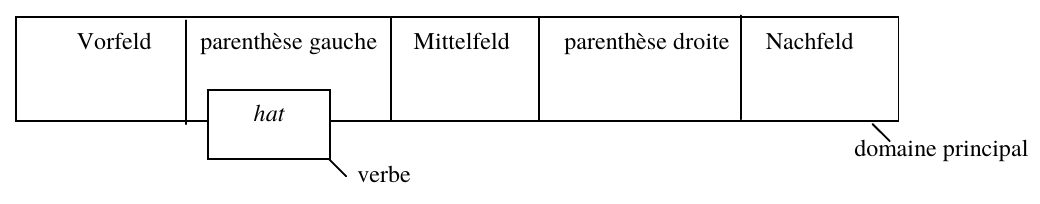
\includegraphics[width=\textwidth]{figures/vol1syntaxe2-img032.png}
   \begin{figure}[H]
      \begin{tabular}{|c|c|c|c|c|}
      \hline
      \multicolumn{5}{|c|}{\cellcolor{lsDOIGray}Domaine principal}\\
      \hline
      & {\cellcolor{lsDOIGray}parenthèse} &  & {parenthèse} & \\
       Vorfeld        & {\cellcolor{lsDOIGray}gauche}     &     Mittelfeld       &  droite      & Nachfeld \\
      \hline
      \end{tabular}
    \caption{Gabarit topologique du domaine principal de l'allemand\label{fig:gabarit-allemand}}
    \end{figure}

    Le verbe principal de la phrase, c’est-à-dire le verbe qui porte le mode indicatif, se place dans la 2\textsuperscript{e} position, appelée \hi{parenthèse gauche}, après l’unique constituant occupant le \hi{champ initial} ou \hi{Vorfeld} ‘pré-champ’. Les dépendants verbaux vont généralement dans la \hi{parenthèse droite}. La parenthèse gauche entoure avec la parenthèse droite, le \hi{champ du milieu} ou \hi{Mittelfeld}. Un \hi{champ final} ou \hi{Nachfeld} suit la parenthèse droite. Les \hi{champs} dits \hi{majeurs} -- Vorfeld, Mittelfeld et Nachfeld -- accueillent les différents groupe substantivaux ou adverbiaux. 
    
    Considérons la phrase \REF{ex:leider} et son arbre de dépendance, donné dans la figure~\ref{fig:leider}.
    
    \ea\label{ex:leider}
    \gll Leider hat Peter {mal wieder} in seiner Nase zu popeln gewagt   vor der ganzen Familie.\\
         Hélas   a   Peter   {une fois de plus}   dans son nez   de creuser osé   devant toute la famille\\
    \glt ‘Peter a malheureusement osé à nouveau se crotter le nez devant toute la famille.’
    \z
    
    La racine de l'arbre de \REF{ex:leider}, l'auxiliare \textit{hat} `a' va dans la parenthèse gauche, tandis que le participe \textit{gewagt} 'osé' va dans la parenthèse droite, où il entraîne avec lui le verbe infinitif \textit{zu popeln} `de creuser', qui se place devant lui. Les verbes de la parenthèse droite ne peuvent pas accueillir leur dépendants substantivaux et adverbiaux, qui vont donc s'émanciper et se placer dans le domaine principal. Un des constituants doit occuper le Vorfeld : ici c'est \textit{leider} qui occupe cette place, mais n'importe quel autre constituant aurait pu prendre la place.
    Le constituant \textit{vor der ganzen Familie} ‘devant toute la famille’ peut aller dans le Nachfeld, car il est assez lourd (et un placement dans le Mittelfeld séparerait trop les deux parenthèses). Des constituants légers comme \textit{mal wieder} ou le sujet \textit{Peter} préfèrent rester dans le Mittelfeld.
    
    
    \begin{figure}[H]
      \caption{Arbre de dépendance de \REF{ex:leider}\label{fig:leider}}
    \begin{forest} for tree={font=\itshape}
      [hat
        [leider]
        [Peter]
        [gewagt
            [mal wieder]
            [zu popeln 
                [in seiner Nase]
                [vor der ganzen Familie]
            ]
        ]
      ]
    \end{forest}
   \end{figure}
    

    Les propositions subordonnées, complétives et relatives, ont une structure réduite, sans Vorfeld, et l’élément qui introduit la proposition, le complémenteur ou le pronom relatif, occupe la parenthèse gauche. En conséquence, le verbe principal de la subordonnée va dans la parenthèse droite.

    \ea\label{ex:glaube}
    \gll  Ich glaube,   {\ob} dass Peter {mal wieder} in seiner Nase zu {popeln\textsubscript{3}} {gewagt\textsubscript{2}} {hat\textsubscript{1}}   {\cb}.\\
    Je crois   [ que  Peter {une fois de plus} dans son nez   de creuser  osé        a   ]\\
    \glt ‘Je crois que Peter a osé se crotter le nez à nouveau.’
    \z
    
    Dans l'exemple \REF{ex:glaube}, il y a trois verbes dans la parenthèse droite de la subordonnée, que nous avons numéroter de 1 à 3 pour bien montrer que c'est le verbe principal qui est en dernier.
    Le placement des verbes dans la parenthèse droite est contraint et peut aussi être décrit par une structure topologique, que nous nommons l’\textit{amas verbal}. Il est composé de trois champs : le \hi{champ supérieur} ou \hi{Oberfeld}, le champ tête et le \hi{champ inférieur} ou \hi{Unterfeld} (voir la figure~\ref{fig:topo-amas-allemand}). Le placement le plus courant est celui illustré en \REF{ex:glaube}, où chaque verbe subordonné se place à gauche de son gouverneur, c'est-à-dire dans le champ Oberfeld.

    \begin{figure}[H]
    \def\arraystretch{1.5}
    \setlength{\tabcolsep}{4ex}
    \begin{tabular}{|c|c|c|}
    \hline
    \multicolumn{3}{|c|}{\cellcolor{lsDOIGray}Amas verbal}\\
    \hline
    Oberfeld & \cellcolor{lsDOIGray}champ tête & Unterfeld\\
    \hline
    \end{tabular}
    \caption{Gabarit topologique de l'amas verbal en l'allemand\label{fig:topo-amas-allemand}}
    \end{figure}
    
    Sans rentrer dans tous les détails de l’amas verbal, remarquons que pour certains verbes, en particulier les modaux, le placement dans l’Unterfeld est préférable à l’Oberfeld :

    \ea\label{ex:konnen}
    \ea[\textsuperscript{?}]{
    \gll Ich glaube,  {\ob} dass Peter {mal wieder} in seiner Nase {popeln\textsubscript{3}} {gekonnt\textsubscript{2} } {hat\textsubscript{1}}   {\cb}.\\
        Je crois  [ que   Peter {une fois de plus} dans son nez   creuser  pu           a   ]\\}
    \ex[]{
    \gll Ich glaube,  {\ob} dass Peter {mal wieder} in seiner Nase {hat\textsubscript{1}} {popeln\textsubscript{3}} {können\textsubscript{2}}   {\cb}.\\
    Je crois   [ que   Peter {une fois de plus} dans son nez  a     creuser  pu   ]\\
    \glt  ‘Je crois que Peter a pu se crotter le nez à nouveau.’}
    \z
    \z
    Dans l’exemple (\ref{ex:konnen}a), on observe l’ordre standard dans la parenthèse droite : l’infinitif \textit{popeln} ‘creuser’ se place dans l’Oberfeld du participe \textit{gekonnt} ‘pu’, lui-même placé dans l’Oberfeld de l’auxiliaire \textit{hat} ‘a’. On préfère en fait b, où un «~ersatz~» d’infinitif (all. \textit{Ersatzinfinitiv}), \textit{können} ‘pouvoir’, est réalisé au lieu du participe et où celui-ci est placé dans l’Unterfeld de l’auxiliaire, tandis que \textit{popeln} ‘creuser’ se place à nouveau dans l’Oberfeld de son gouverneur. Cette construction est appelée l’\textit{Oberfeldumstellung} ‘conversion du champ supérieur’. Pour certains locuteurs de l’allemand, le verbe \textit{popeln} peut se placer dans l’Oberfeld de l’auxiliaire, non occupé par le dépendant direct de l’auxiliare. Cette nouvelle construction, avec l’auxilaire entre les deux verbes à l’infinitif, est appelée le \textit{Zwischenstellung} ‘positionnement intermédiaire’ :

    \begin{exe}
    \exr{ex:konnen}
    \begin{xlist}
    \exi{c.} \gll Ich glaube,  {\ob} dass Peter {mal wieder} in seiner Nase  {popeln\textsubscript{3}} {hat\textsubscript{1}} {können\textsubscript{2}} {\cb}.\\
    Je crois   {\ob} que   Peter {une fois de plus} dans son nez  creuser  a     pu {\cb}\\
    \glt ‘Je crois que Peter a pu se crotter le nez {une fois de plus}.’
    \end{xlist}
    \end{exe}
}
\loupe[sec:3.5.37]{L’anglais comme langue de référence}{%
    Peu d’approches théoriques distinguent, comme nous le faisons, la structure syntaxique de la structure topologique. Nous pensons que la non-prise en compte de la topologie doit beaucoup au fait que l’anglais sert de langue de communication dans le monde scientifique et donc de langue de référence de très nombreux travaux en linguistique. Or l’anglais est, du point de vue typologique (c’est-à-dire lorsqu’on prend en compte la diversité des langues), une langue particulièrement «~exotique~». En effet, l’anglais a un ordre des mots singulièrement rigide, avec non seulement une position fixe du sujet devant le verbe, mais aussi l’obligation de placer l’objet direct avant les autres compléments. Cette particularité permet de postuler une sorte de groupe verbal (voir l’\encadref{sec:3.4.20} sur \textit{Le groupe verbal}) au niveau topologique en anglais. 
    
    Le fait que la structure syntaxique et la structure topologique soient si fortement liées en anglais peut amener à les identifier et donc à considérer aussi un constituant syntaxique VP (\textit{verb phrase}) au niveau syntaxique, comme le font les générativistes. Mais, cela va plus loin, car les mêmes générativistes considèrent que toutes les langues devraient avoir un VP. Les langues qui autorisent le placement du sujet entre le V et l’objet, contredisant de fait l’existence d’un VP, sont alors dites \hi{non-configurationnelles}. Certains linguistes, dont Chomsky, considèrent qu’il y a bien un VP sous-jacent, mais que les syntaxèmes sont systématiquement déplacés en surface (voir l’\encadref{sec:3.2.6} sur \textit{Linéarisation et mouvement}). C’est une analyse que nous rejetons totalement.
}
\chevalier[sec:3.5.38]{Historique de la description topologique}{%
    Nous avons déjà mentionné à deux reprises la contribution de Gabriel \citet{girard1747vrais} à la modélisation de l’ordre des mots. Son ouvrage contient une dizaine de \hi{règles de précédence linéaire} remarquablement formalisées. Par exemple :

    \begin{quote}
    «~Première Règle. – Dans la forme expositive, le Subjectif marche ordinairement devant l’Attributif : celui-ci y précède à son tour l’Objectif et le Terminatif, lorsqu’ils sont énoncés par des expressions formelles et non simplement désignés par des pronoms personnels ou relatifs.~»
    \end{quote}
    Cette règle indique que, dans la phrase déclarative (= expositive), le sujet (= Subjectif) se place devant le prédicat verbal (= Attributif), qui lui-même précède l’objet direct (= Objectif) et l’objet indirect (= Terminatif), à moins que ceux-ci ne soient des pronoms personnels ou relatifs. Les règles suivantes de Girard indiquent que le sujet se place après le verbe dans les propositions en incise (Règle II), que le sujet peut se placer après le verbe en l’absence d’un objet direct ou quand celui-ci est un pronom (Règle III), etc.

    Le modèle topologique, avec ses gabarits de places fixes, s’est développé au siècle suivant en Allemagne. Simon \citet{herling1821uber} propose la première théorie globale sur la structure hiérarchique des phrases complexes de l’allemand basée sur des gabarits de places fixes. Oskar \citet{erdmann1886grundzuge} poursuit le travail de Herling en énumérant les types d’éléments que ces places peuvent contenir, donnant ce que \citet{Höhle1986} propose d’appeler le système de Herling-Erdmann et qu’on appelle plus souvent aujourd’hui la \textit{théorie des champs topologiques}. Le terme \textit{Feld} ‘champ’ pour désigner ces places dans la phrase apparaît pour la première fois chez Erich \citet{drach1937grundgedanken} dans un livre intitulé~\textit{Grundgedanken der Deutschen Satzlehre} ‘Idées fondamentales de la phrase allemande’ destiné aux enseignants de l’allemand comme langue maternelle et langue étrangère. Le livre de Drach prône, avec une teinte légèrement nationalisante propre à l'époque, une émancipation de la grammaire allemande, qui était jusqu’à là sous une influence latine forte, en faveur d’une «~construction d’une présentation et d’un système de règles basé sur la nature de la langue allemande~». Gunnar \citet{bech1955studien} a adapté par la suite la terminologie de Drach pour décrire la structure interne de l'amas verbal.

    Le modèle topologique a été appliqué par Povl \citet{skaarup1975premieres} à la description de l’ordre des mots en ancien français, montrant l’influence des langues germaniques sur l’émergence du français contemporain. \citet{gerdes2006amas} proposent le modèle topologique pour le français présenté dans ce chapitre, qui s’appuie notamment sur les travaux sur la macrosyntaxe de Claire \citet{blanche-benveniste1990francais}. Le modèle topologique a aussi été appliqué à des langues clairement non germaniques, comme dans la description par \citet{DonohueSag1999} du warlpiri, une langue aborigène d’Australie à ordre très libre.

    La question de l’ordre des mots a été peu traitée dans les premières grammaires formelles. Dans les grammaires de constituants, l’ordre linéaire est intégré à la structure syntaxique et toute variation de l’ordre des mots suppose un changement de structure syntaxique (voir l’\encadref{sec:3.2.7} \textit{De la non-séparation des ordres au mouvement}). Il faudra attendre le début des années 1980 pour que soient proposées des grammaires de constituants où les \hi{règles de précédence linéaire} sont séparées des règles de sous-catégorisation, notamment avec le modèle GPSG (\textit{Generalized Phrase Structure Grammar}, \citealt{gazdar1985generalized}), qui donnera ensuite HPSG (\textit{Head-driven Phrase Structure Grammar}, \citealt{PollardSag1987}). Le modèle topologique de l’allemand sera formalisé pour la première fois par Andreas \citet{kathol1995linearization-based} dans le cadre de HPSG.

    Dans le cadre des grammaires de dépendance, \citet{melcuk1987surface} proposent une liste très complète des constructions de l’anglais et des règles de précédence linéaire qui vont avec. Le modèle topologique sera formalisé en grammaire de dépendance simultanément par \citet{duchier2001topological} et \citet{gerdes2001word} (voir la formalisation proposée dans l’\encadref{sec:3.5.33} sur la \textit{Grammaire topologique formelle}).
}
\exercices{%\label{sec:3.5.39}
    \exercice{1} 
    \begin{enumerate}[label=\alph*.]
    \item Qu’est-ce que la topologie ?
    \item À quel endroit du modèle linguistique le modèle topologique intervient-il dans un modèle stratificationnel comme la théorie Sens-Texte (voir la \sectref{sec:1.3.8} \textit{Modularité et stratification} et l'\encadref{sec:1.3.9} \textit{La Théorie Sens-Texte}) ?
    \item Pourquoi rejetons-nous la notion d’ordre de base ?
    \end{enumerate}

    \exercice{2} (Ordre préfixé et postfixé.)
    \begin{enumerate}[label=\alph*.]
    \item On considère l’expression préfixée × 3 + × 12 5 7. Donner l’arbre de dépendance correspondant et en déduire une expression infixée et postfixée.

    \item On considère l’expression postfixée 1 5 ${\surd}$ + 2 /. Sachant que ${\surd}$ (racine carrée) est un opérateur unaire (c’est-à-dire d’arité 1), donner l’arbre de dépendance correspondant à cette expression. En déduire l’écriture traditionnelle de ce nombre (qui n’est autre que le nombre d’or).
    \end{enumerate}
    \exercice{3} (Projectivité.) Construire la structure de dépendance de la phrase suivante et vérifier qu’elle est non projective :

    \begin{exe} \exi{} À \textit{cette heure-là, je pense qu’il est déjà parti.} \end{exe}

    \exercice{4} (Théorie des graphes.) Le graphe K\textsubscript{4} n’est pas planaire extérieur (voir l'\encadref{sec:3.5.15} sur \textit{Projectivité et planarité}). Montrer qu’il est néanmoins planaire et que donc tous les graphes de 4 nœuds ou moins sont planaires. Chercher les graphes non-planaires les plus simples à 5 et à 6 nœuds.

    \exercice{5} (Topologie du groupe substantival en français.) On s’intéresse plus particulièrement au placement des déterminants et des numéraux en français. Comment rendre compte des données suivantes dans un modèle topologique ?

    \begin{exe}
    \sn
    \begin{xlista}
    \ex[]{\itshape les/mes/ces/deux/quelques/des/plusieurs amis sont venus}
    \ex[]{\itshape les/mes/ces deux/quelques amis sont venus}
    \ex[*]{\itshape les mes/ces/des/plusieurs amis sont venus}
    \ex[*]{\itshape amis sont venus}
    \end{xlista}
    \end{exe}

    \exercice{6} (Interrogation en français.) On observe un contraste entre le fonctionnement des interrogatifs \textit{à qui} et \textit{que~}:
    
    \begin{exe}
    \sn
    \begin{xlista}
    \ex[]{\itshape À qui parle-t-elle ?}
    \ex[]{\itshape À qui Marie parle-t-elle ?}
    \ex[]{\itshape Que dit-elle ?}
    \ex[*]{\itshape Que Marie dit-elle ?}
    \end{xlista}
    \end{exe}
    Comment expliquer cette différence de comportement dans le cadre d’un modèle topologique ?

    \exercice{7} (Topologie de l’anglais.) L’anglais possède une classe de verbes que l’on appelle les \terme{modaux} qui comprend les auxiliaires \textsc{be} ‘être’ et \textsc{have} ‘avoir’ et quelques verbes à valeur modale, comme \textsc{can} ‘pouvoir’, \textsc{must} ‘devoir’, \textsc{will} (auxiliaire du futur) ou \textsc{would} (auxiliaire du conditionnel), qui ont la particularité d’être invariables, ainsi que la proforme \textsc{do} ‘faire’. Ces verbes ont également des propriétés distributionnelles qui les distinguent des autres verbes. Premièrement, les adverbes se placent de préférence après les modaux et avant les verbes ordinaires :
    
    \begin{exe}
    \exi{(i)}
    \judgewidth{\textsuperscript{??}}
    \begin{xlista}
    \ex[]{\textit{Mary often calls Peter.}     ‘Marie appelle souvent Pierre.’}
    \ex[\textsuperscript{??}]{\textit{Mary calls often Peter.}}
    \ex[]{\textit{Mary would often call Peter.}   ‘Marie appellerait souvent Pierre.’}
    \ex[\textsuperscript{??}]{\textit{Mary often would call Peter.}}
    \end{xlista}
    \end{exe}
    Deuxièmement, dans les interrogatives, le sujet se place entre le modal et le verbe, et en cas d’absence de modal, \textsc{do} est introduit :
    
    \begin{exe}
    \exi{(ii)}
    \begin{xlista}
    \ex[]{\textit{Would Mary call Peter?}     ‘Marie appellerait-elle Pierre ?’}
    \ex[*]{\itshape Calls Mary Peter?}
    \ex[]{\textit{Does Mary call Peter?}     ‘Marie appelle-t-elle Pierre ?’}
    \end{xlista}
    \end{exe}
    La position initiale peut aussi être occupée par un pronom interrogatif :
    
    \begin{exe}
    \exi{(iii)}
    \begin{xlista}
    \ex[]{\textit{Why would Mary call Peter?}   ‘Pourquoi Marie appellerait-elle Pierre ?’}
    \ex[]{\textit{Who does Mary call?}     ‘Qui Marie appelle-t-elle ?’}
    \end{xlista}
    \end{exe}
    Troisièmement, la négation se place obligatoirement sur un modal et donc comme dans le cas de l’interrogation, \textsc{do} doit être introduit en l’absence d’un autre modal :
    
    \begin{exe}
    \exi{(iv)}
    \begin{xlista}
    \ex[]{\textit{Mary would not call Peter.}     ‘Marie n’appellerait pas Pierre.’}
    \ex[*]{\itshape Mary calls not Peter.}
    \ex[]{\textit{Mary does not call Peter.}    ‘Marie n’appelle pas Pierre.’}
    \end{xlista}
    \end{exe}
    Quatrièmement, le sujet peut être inversé dans certains cas :
    
    \begin{exe}
    \exi{(v)}
    \begin{xlista}
    \ex  \textit{Never does Mary call Peter.}   ‘Jamais Marie n’appelle Pierre.’
    \ex  \textit{Here are two nice people.}     ‘Ici sont deux chouettes personnes.’
    \end{xlista}
    \end{exe}
    Rappelons également que, en anglais, l’objet direct doit précéder tous les autres compléments. De quelle façon un modèle topologique de l’anglais peut-il rendre compte de ces propriétés ?

    \exercice{8} (Topologie de l’allemand.) Les exemples que nous avons présentés dans l’\encadref{sec:3.5.36} acceptent encore d’autres ordres, comme, par exemple :

    \begin{exe}
    \sn
    \gll In seiner Nase zu popeln hat Peter {mal wieder} gewagt.\\
         dans son nez  de creuser  a   Peter   {une fois de plus}   osé\\
    \glt   ‘Peter a à nouveau osé se crotter le nez.’
    \end{exe}
  Comment pouvez-vous intégrer cet exemple au modèle topologique de l’allemand ?

    \exercice{9} Ce que nous avons fait pour le français, l’allemand, le russe ou l’anglais peut être fait pour n’importe quelle langue a priori. Nous avons déjà écrit des modèles topologiques pour l’arabe, le chinois ou le wolof. Vous pouvez essayer d’écrire un fragment de modèle topologique pour la langue de votre choix et nous l’envoyer.
}
\lecturesadditionnelles{% \label{sec:3.5.40}
    Comme nous l’avons déjà mentionné au \chapref{sec:3.3}, on peut consulter en ligne la plupart des ouvrages anciens. On trouvera facilement \citet{buffier1709grammaire}, \citet{girard1747vrais}, \citet{gaultier1817atlas}, \citet{weil1844de}, ainsi que les articles de Beauzée et Dumarsais dans l’\textit{Encyclopédie} de Diderot et D’Alembert (voir le \chapref{sec:3.3}).

    Les premiers travaux sur le modèle topologique sont en allemand : \citet{erdmann1886grundzuge}, \citet{drach1937grundgedanken}, \citet{bech1955studien}. Pour des travaux plus récents sur l’ordre des mots, nous avons mentionné \citet{gazdar1985generalized}, \citet{pollard1994head-driven}, \citet{melcuk1987surface}, \citet{kathol1995linearization-based}, ainsi que les articles de \citet{bresnan2007predicting}, \citet{duchier2001topological} et \citet{gerdes2001word,gerdes2006amas}. Sur la structure communicative et son rôle dans l’ordre des mots, nous renvoyons à \citet{lambrecht1996information} et \citet{melcuk2001communicative}.

    Pour les travaux typologiques sur l’ordre des mots, on consultera l’article original de \citet{greenberg1963universals} et l’étude et le travail très complet de \citet{dryer1992greenbergian}, ainsi que les cartes et les différents articles consacrés à l’ordre des mots sur le site \url{https://wals.info}, une base de données typologique où sont répertoriés 192 traits pour plus de 2500 langues (\citealt{haspelmath2005world}) !

    \FurtherReading{3-5}
}
\pagebreak\largerpage
\corrections{%\label{sec:3.5.41}
    \corrigé{1}
    \begin{enumerate}[label=\alph*.]
    \item La topologie est l’étude du placement des unités syntaxiques, c’est-à-dire l’étude de l’ordre des mots, mais aussi des syntaxèmes à l’intérieur des mots.

    \item Le modèle linguistique décrit la correspondance entre le sens et le texte. Le modèle topologique décrit la linéarisation, c’est-à-dire la correspondance entre la structure syntaxique (non ordonnée) et la chaîne linéaire. Ou dans sa version plus élaborée entre une structure de dépendance syntaxique et un arbre de constituants topologiques.

    \item Certaines langues ont un ordre dominant, comme l’ordre SVO en français. Néanmoins considérer un ordre de base revient à considérer que tous les autres ordres sont obtenus par des transformations de l’ordre base. Cela revient à dire que lorsque le sujet est après le verbe en français, celui-ci a été inversé. Même s’il peut nous arriver de conserver la terminologie et de parler de «~sujet inversé~», nous ne considérons pas qu’il y a eu une inversion. Nous considérons que le sujet a été placé directement dans cette position. La notion d’ordre de base est directement liée à des modèles, comme la grammaire générative, qui ne considère pas de structure syntaxique dissociée d’un ordre linéaire sur les mots.
    \end{enumerate}
    \corrigé{2} 
    \begin{enumerate}[label=\alph*.]
    \item Le premier symbole, $\times$, est la racine de l’arbre. Son premier dépendant est 3. Le symbole suivant, +, est la racine du deuxième dépendant, et ainsi de suite. La formule est donc $3 \times \left((12\times5) + 7\right)$ sous forme infixée et 3 12 5 $\times$ 7 + $\times$ sous forme postfixée. 

    \item La formule est (1 + $\sqrt{5}$) / 2 sous forme infixée et / + 1 $\surd$ 5 2 sous forme préfixée.
    \end{enumerate}

    \corrigé{3} Le syntagme \textit{à cette heure-là} dépend de \textit{parti} et couvre donc la racine de l’arbre \textit{pense}.

    \corrigé{4} Le graphe K\textsubscript{4} est planaire : il suffit de prendre une des diagonales et de la faire passer par l’extérieur du carré. C’est le plus complexe des graphes à 4 nœuds et donc tous les graphes à 4 nœuds ou moins sont planaires. Le plus petit graphe non planaire à 5 nœuds est K\textsubscript{5}, le graphe complet à 5 nœuds. Le plus petit graphe non planaire à 6 nœuds est K\textsubscript{3,3}, le graphe où 3 nœuds sont liés aux 3 autres (voir la figure~\ref{fig:K5}). On vérifiera que, si on retire un seul de leurs liens, ces graphes deviennent planaires.

 \begin{figure}[H]
 \caption{Les plus petits graphes non planaires\label{fig:K5}}
    \begin{center}
    \begin{minipage}[c]{.5\linewidth}\centering
      \begin{tikzpicture}
      \begin{scope}[local bounding box=graph,every node/.style={CircleNode}]
        \graph [clockwise, empty nodes] { subgraph K_n [n=5] };
      \end{scope}
        \node[below=1pt of graph] {K\textsubscript{5}};
      \end{tikzpicture}
    \end{minipage}\begin{minipage}[c]{.5\linewidth}\centering
      \begin{tikzpicture}
      \begin{scope}[local bounding box=graph,every node/.style={CircleNode}]
        \graph [empty nodes, branch right, grow down] { subgraph K_nm [n=3, m=3] };
      \end{scope}
        \node[below=1pt of graph] {K\textsubscript{3, 3}};
      \end{tikzpicture}
    \end{minipage}
    \end{center}
    \end{figure}

    Le mathématicien polonais Kazimierz Kuratowski a établi en \citeyear{kuratowski1930probleme} la caractérisation suivante des graphes planaires : un graphe est \hi{planaire} si et seulement s’il ne peut être réduit ni à K\textsubscript{5}, ni à K\textsubscript{3,3}.

    On pourra consulter les pages de la wikipédia sur les graphes planaires et planaires extérieurs.

    \corrigé{5} On observe trois paradigmes de «~déterminants~» : 1) \textit{les, mes, ces~}; 2) \textit{des, plusieurs~}; 3) \textit{deux, quelques}. Les éléments de types 1 et 3 peuvent cooccurrer, tandis que ceux de types 2 excluent les autres. Les noms communs doivent obligatoirement être accompagnés d’au moins un éléments d’un de ces trois types. Les éléments de type 1 sont les déterminants définis, ceux de type 2 les déterminants indéfinis. Quant à ceux de type 3, ce sont des quasi-déterminants, puisqu’ils peuvent se placer entre un déterminant défini et le nom et qu’ils n’ont pas de valeur intrinsèquement définie ou indéfinie, mais ils prennent une valeur indéfinie en l’absence d’un déterminant défini. On peut modéliser cette distribution en considérant deux champs topologiques : un pour les déterminant définis, suivi d’un pour les quasi-déterminants, avec la condition qu’un des deux champs au moins doit être occupé. Les déterminants indéfinis occuperaient quant à eux les deux champs en même temps. (Ou ce qui revient au même, ils occupent le champ des quasi-déterminants, mais excluent, pour des raisons sémantiques, la cooccurrence avec un déterminant défini.)

    \corrigé{6} Les pronoms interrogatifs se placent au début du domaine microsyntaxique, devant le sujet (dans \textit{Marie, à qui parle-t-elle} ?, \textit{Marie} est détaché et n’occupe plus la position sujet). Le pronom interrogatif \textit{que} est la forme faible du pronom \textit{quoi} (comme \textit{me} avec \textit{moi}). C’est un clitique qui doit obligatoirement être dans l’amas verbal (comme \textit{me}). Autrement dit, le pronom interrogatif \textit{que} doit à la fois être en tête du domaine microsyntaxique et dans l’amas verbal, ce qui écrase tout ce qui se trouve entre les deux et en particulier le champ initial qu’occuperait le sujet. Nous développerons une analyse similaire dans le \chapfuturef{19} sur l’\textit{Extraction} pour expliquer les différences d’ordre entre propositions principale et relative.

    \corrigé{7} Les modaux de l’anglais occupent un champ topologique différent de celui des verbes. Le domaine microsyntaxique de la phrase déclarative est donné dans la figure~\ref{fig:domaine-anglais}.
    
    \begin{figure}[H]
      \caption{Domaine verbal microsyntaxique de l'anglais\label{fig:domaine-anglais}}
      \begin{tabular}{|c|c|c|c|c|c|}
        \hline
        \multicolumn{6}{|c|}{\cellcolor{lsDOIGray}Domaine microsyntaxique}\\
        \hline
        ch\_initial & ch\_modal & ch\_adv & ch\_verbal & ch\_objet & ch\_compl\\\hline
      \end{tabular}    
    \end{figure}

    Le sujet va dans le champ initial, sauf quand celui-ci est occupé par un pronom interrogatif, une négation ou un locatif, ou quand il reste vide dans une interrogative totale. Le champ modal peut rester vide quand le sujet occupe le champ initial et qu’il n’y a pas la négation \textit{not} dans le champ adverbial. Lorsque le champ initial est occupé par un autre élément, le sujet va dans le champ adverbial. Dans les interrogatives le sujet ne peut pas occuper le champ initial, qui peut rester vide en l'absence d'un pronom interrogatif. Le champ modal doit obligatoirement être occupé si le sujet n'est pas dans le champ initial.

    \corrigé{8} Cet exemple montre qu’un constituant à tête verbale, comme \textit{in seiner Nase zu popeln} ‘de se crotter le nez’, peut également venir se placer dans le Vorfeld. Nous avons vu un cas similaire dans l'exemple (\ref{ex:Nase-participe}a), où un verbe au participe passé est placé dans le Vorfeld. Il suffit d'indiquer, dans la règle de correspondance de placement dans le Vorfeld, quelles sont la catégories syntaxiques qui sont éligibles.
    Il n’est pas nécessaire d’aménager davantage le modèle.
}


%%%%%%%%%%%%%%%%%%%%%%%%%%%%%%%%%%%%%%%%%%%%%%%%%%%
%%             Backmatter                       %%%
%%%%%%%%%%%%%%%%%%%%%%%%%%%%%%%%%%%%%%%%%%%%%%%%%%%

% \is{some term| see {some other term}}
\il{some language| see {some other language}}
\issa{some term with pages}{some other term also of interest}
\ilsa{some language with pages}{some other lect also of interest}
% % There is normally no need to change the backmatter section
\backmatter
\phantomsection%this allows hyperlink in ToC to work
{\sloppy\printbibliography[heading=french]}
\cleardoublepage

\phantomsection
\addcontentsline{toc}{chapter}{\lsIndexTitle}
\addcontentsline{toc}{section}{\lsNameIndexTitle}
\ohead{\lsNameIndexTitle}
\printindex
\cleardoublepage

\phantomsection
\addcontentsline{toc}{section}{\lsLanguageIndexTitle}
\ohead{\lsLanguageIndexTitle}
\printindex[lan]
\cleardoublepage

\phantomsection
\addcontentsline{toc}{section}{\lsSubjectIndexTitle}
\ohead{\lsSubjectIndexTitle}
\printindex[sbj]
\ohead{}
\cleardoublepage

\end{document}
